\documentclass[UTF8,12pt,a4paper,openany]{ctexbook}
\usepackage[margin=1.7cm]{geometry}
\usepackage{graphicx}
\usepackage{xcolor}
\usepackage[most]{tcolorbox}
\usepackage{hyperref}
\usepackage{fancyhdr}
\usepackage{enumitem}
\hypersetup{colorlinks=true,linkcolor=blue,urlcolor=blue}
\pagestyle{fancy}
\fancyhf{}
\setlength{\headheight}{15pt}
\lhead{结构力学十四讲作业与答案整理}
\rhead{\thepage}
\setlength{\parindent}{2em}
\setlist[itemize]{leftmargin=2em}
\tcbset{colback=gray!4,colframe=black!45,arc=2mm,boxrule=0.5pt}
\title{结构力学十四讲作业与答案整理\\\large 去水印版、解析与讲解笔记汇编}
\author{根据本地资料整理}
\date{\today}
\begin{document}
\maketitle
\frontmatter
\chapter*{整理说明}
本工程将本地 \texttt{6.作业\&答案} 与 \texttt{7.作业讲解笔记} 中的资料整理为 XeLaTeX 可编译文档。原始资料多为手写或扫描式 PDF，机器文本识别不稳定，因此保留去水印、裁边后的页面图像，并为每讲补充解析要点、答案校核提示和对应讲解笔记。
\par 本文按前十四讲组织：第 1--12 讲对应第 1--12 次作业，第 13 讲为弯矩分配法，第 14 讲为矩阵位移法；动力学资料位于原第 15 次作业和第 14 次讲解笔记，未纳入本十四讲主线。
\tableofcontents
\mainmatter
\chapter{第1讲：几何组成分析}
\begin{tcolorbox}[title=解析要点]
几何组成分析先看支座约束和体系自由度，再用二元体规则、两刚片/三刚片规则与瞬变判据逐步化简。答案判断应写清“几何不变、几何可变或瞬变”的理由。
\end{tcolorbox}
\begin{tcolorbox}[title=答案与校核]
答案页给出了几何组成判定过程；整理时以约束数、刚片连接方式和瞬变情形作为最终判据。
\end{tcolorbox}
\section{作业与答案（去水印版）}
\begin{center}
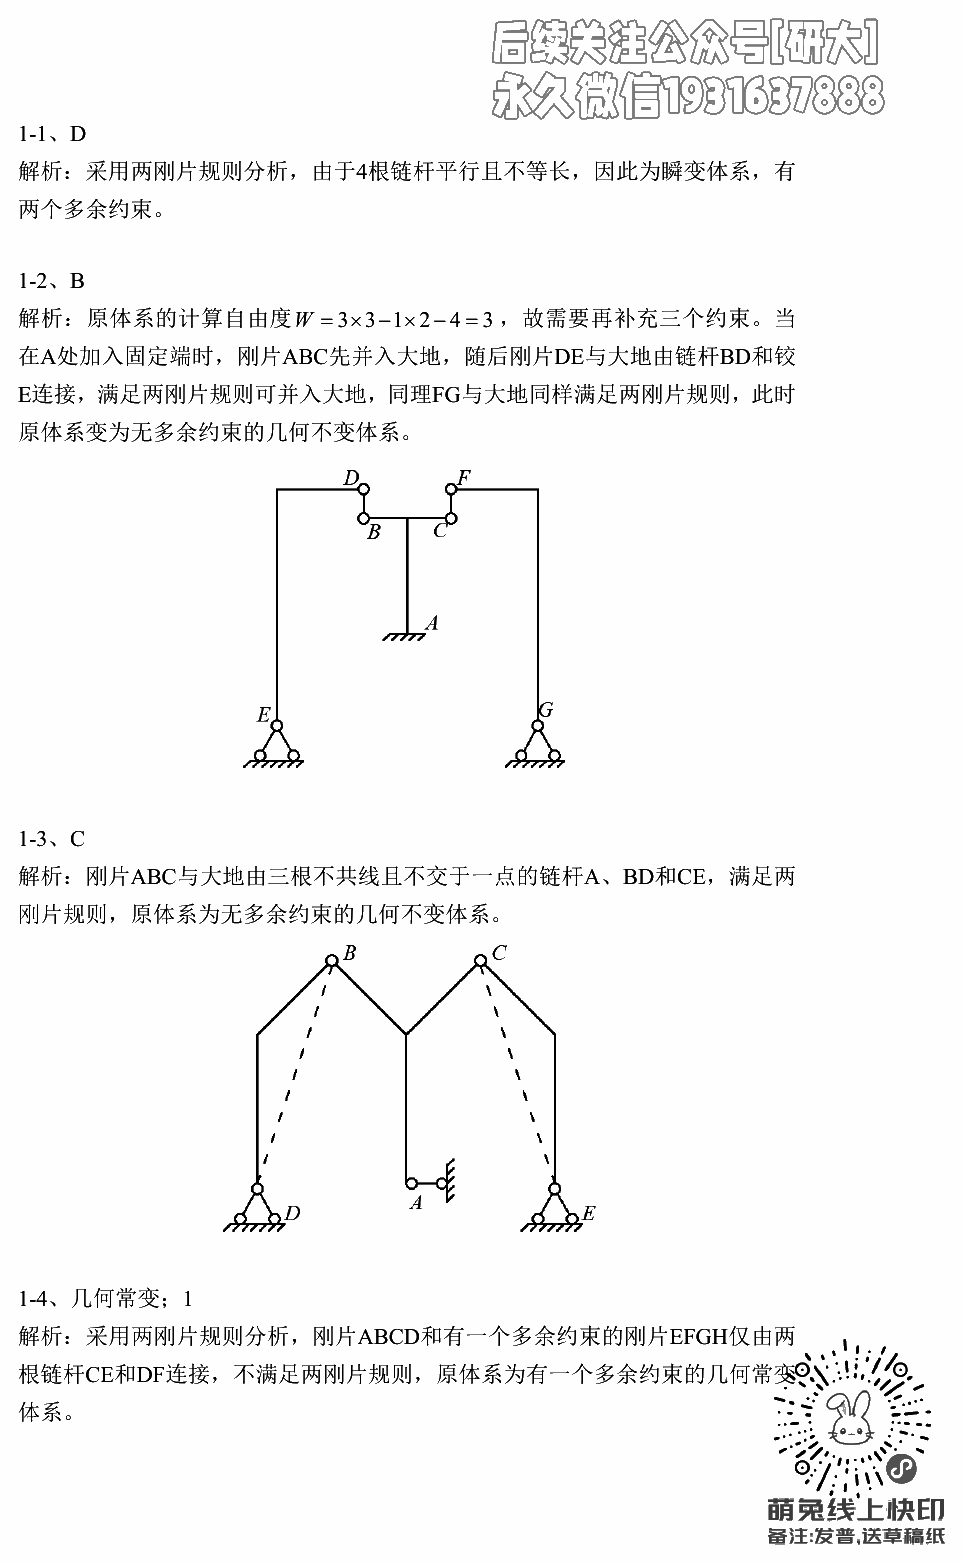
\includegraphics[width=0.96\textwidth,height=0.82\textheight,keepaspectratio]{images/c01_answer_1_p01.png}
\par\small 作业与答案（去水印版），第 1/9 页
\end{center}
\clearpage
\begin{center}
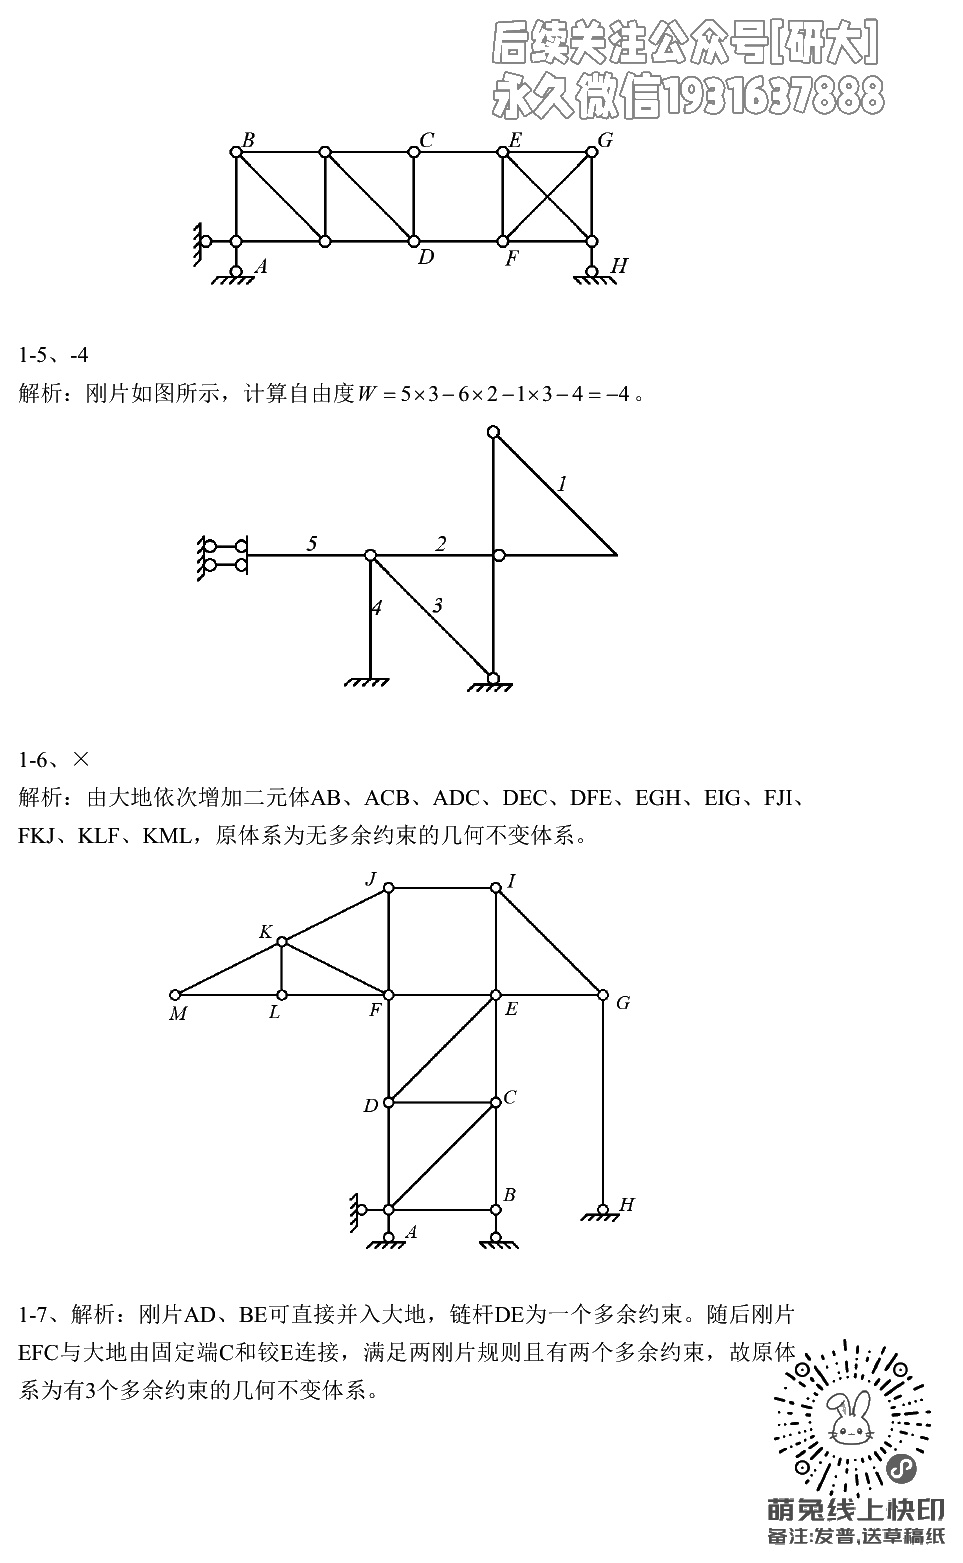
\includegraphics[width=0.96\textwidth,height=0.82\textheight,keepaspectratio]{images/c01_answer_1_p02.png}
\par\small 作业与答案（去水印版），第 2/9 页
\end{center}
\clearpage
\begin{center}
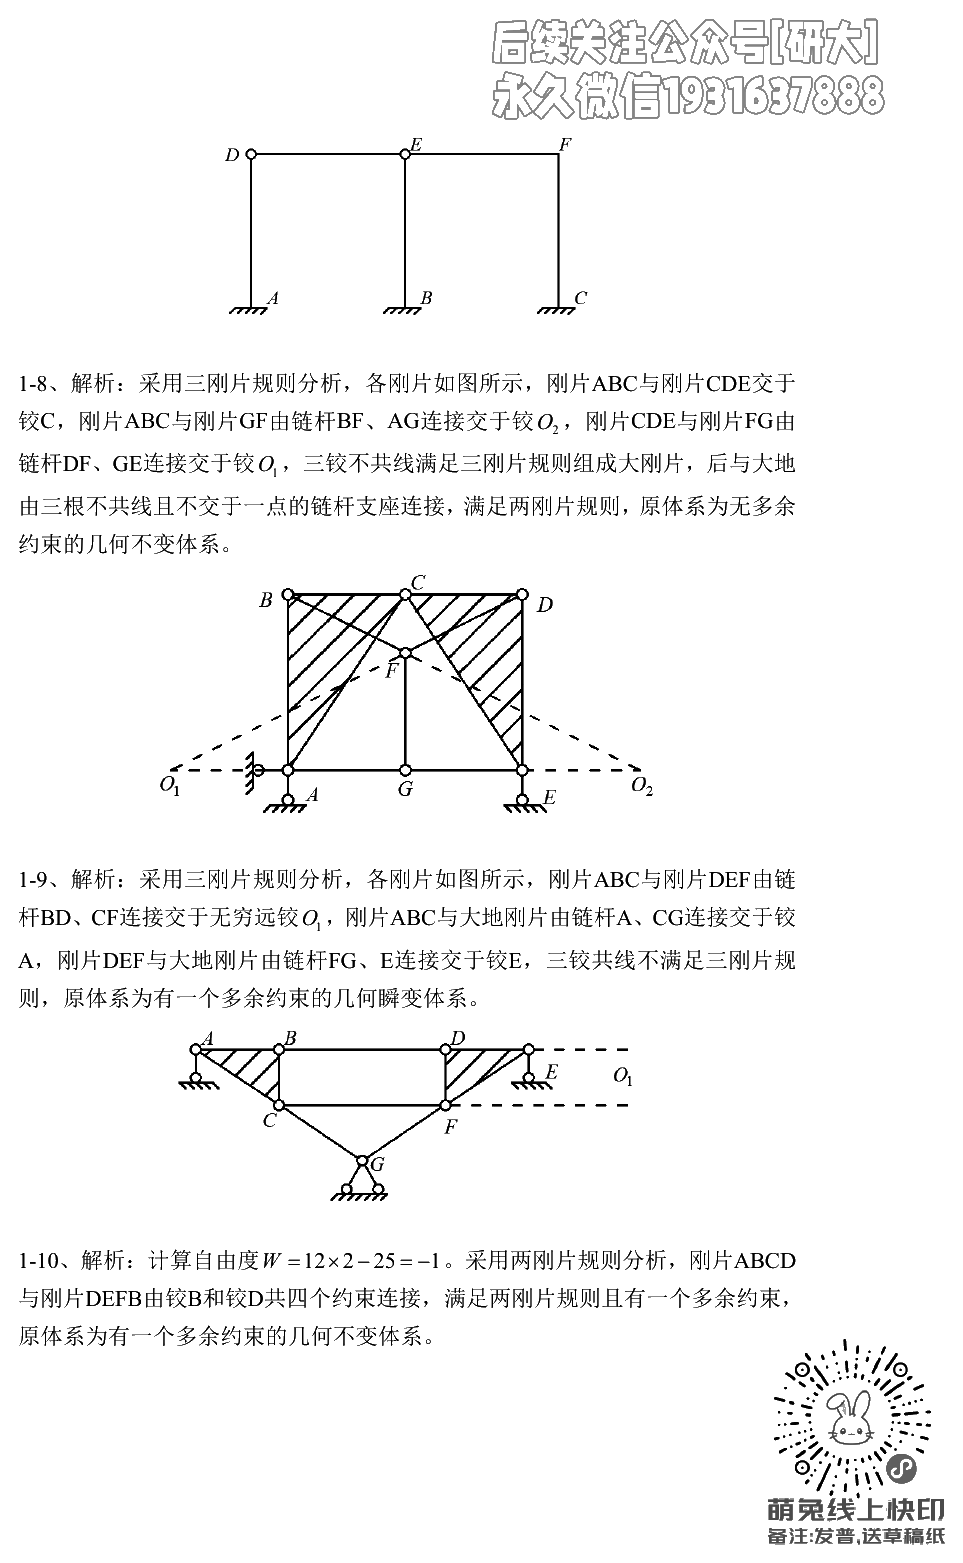
\includegraphics[width=0.96\textwidth,height=0.82\textheight,keepaspectratio]{images/c01_answer_1_p03.png}
\par\small 作业与答案（去水印版），第 3/9 页
\end{center}
\clearpage
\begin{center}
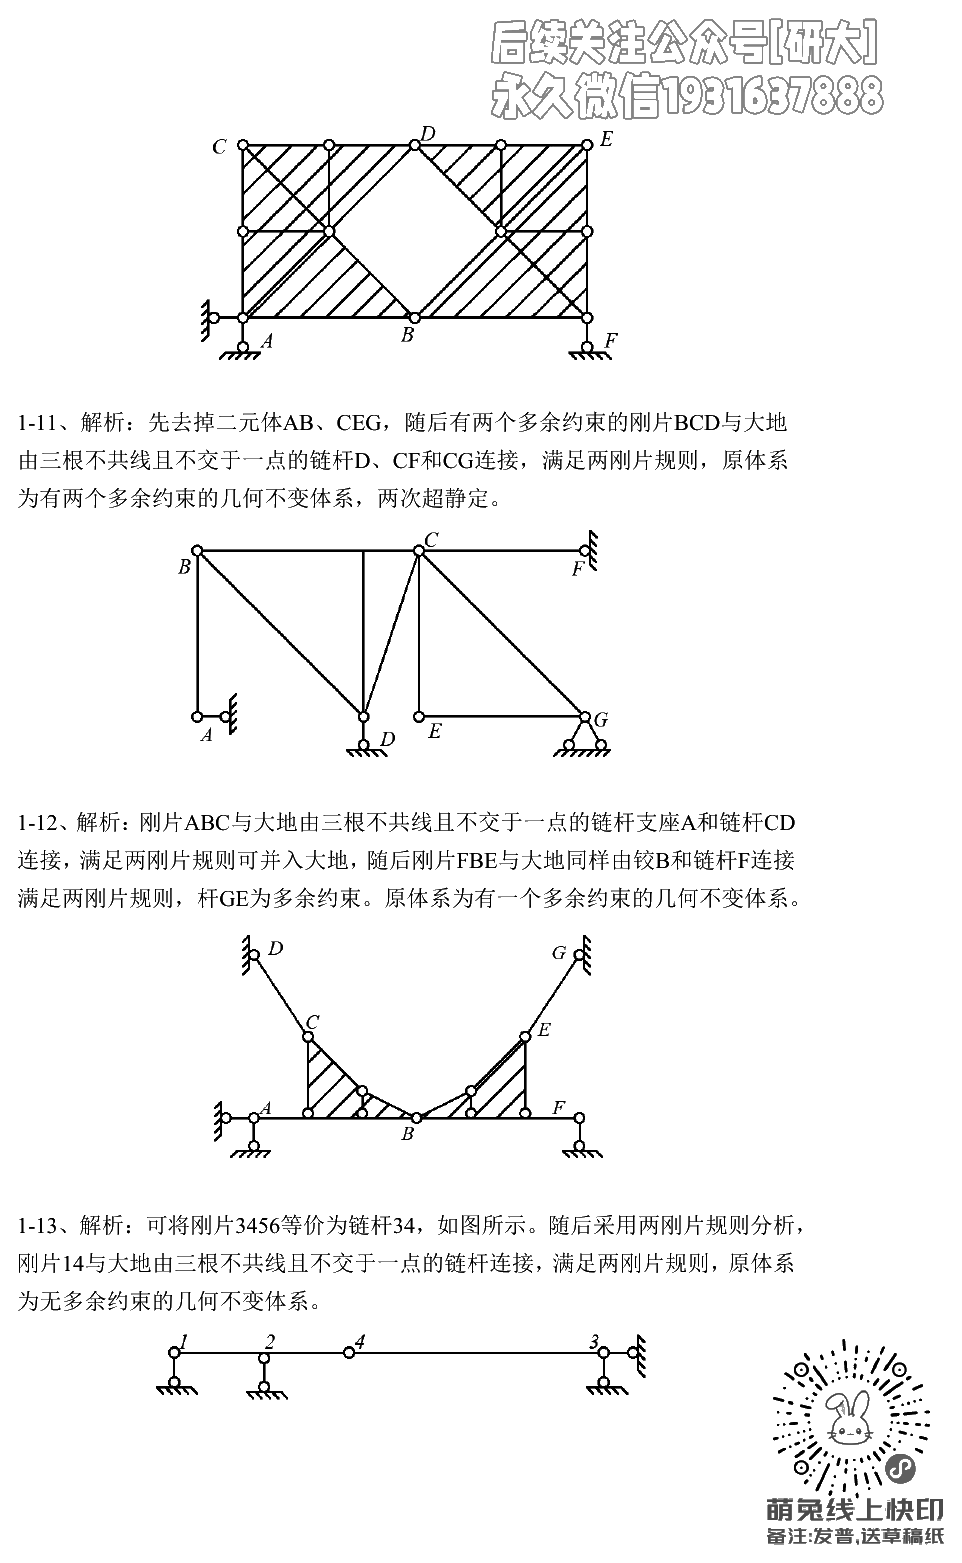
\includegraphics[width=0.96\textwidth,height=0.82\textheight,keepaspectratio]{images/c01_answer_1_p04.png}
\par\small 作业与答案（去水印版），第 4/9 页
\end{center}
\clearpage
\begin{center}
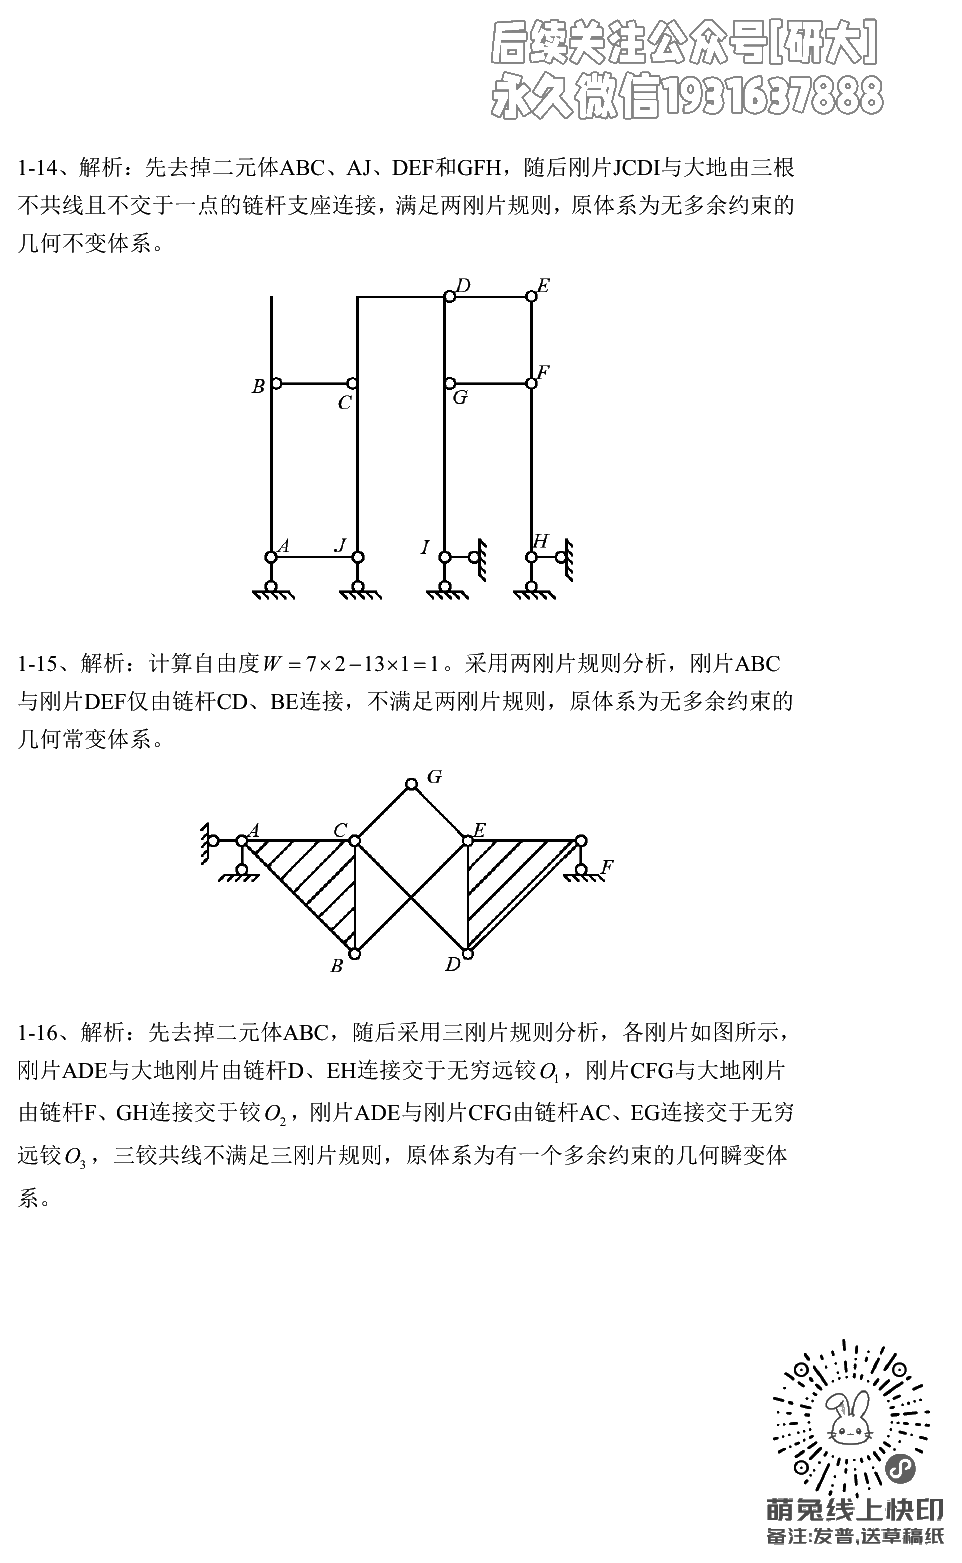
\includegraphics[width=0.96\textwidth,height=0.82\textheight,keepaspectratio]{images/c01_answer_1_p05.png}
\par\small 作业与答案（去水印版），第 5/9 页
\end{center}
\clearpage
\begin{center}
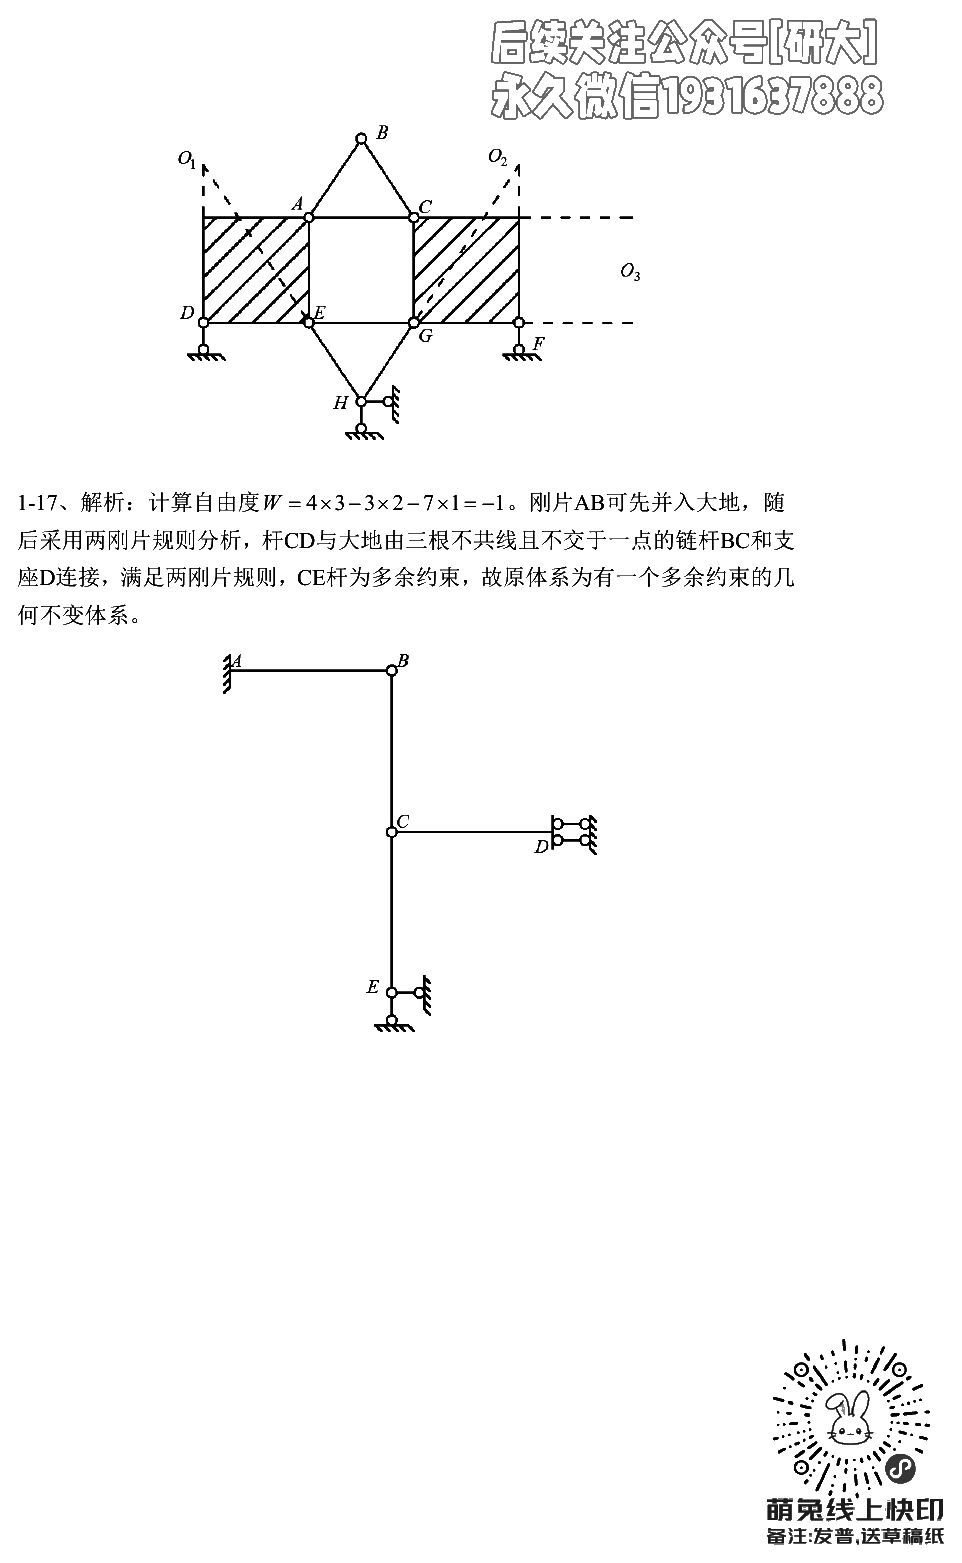
\includegraphics[width=0.96\textwidth,height=0.82\textheight,keepaspectratio]{images/c01_answer_1_p06.png}
\par\small 作业与答案（去水印版），第 6/9 页
\end{center}
\clearpage
\begin{center}
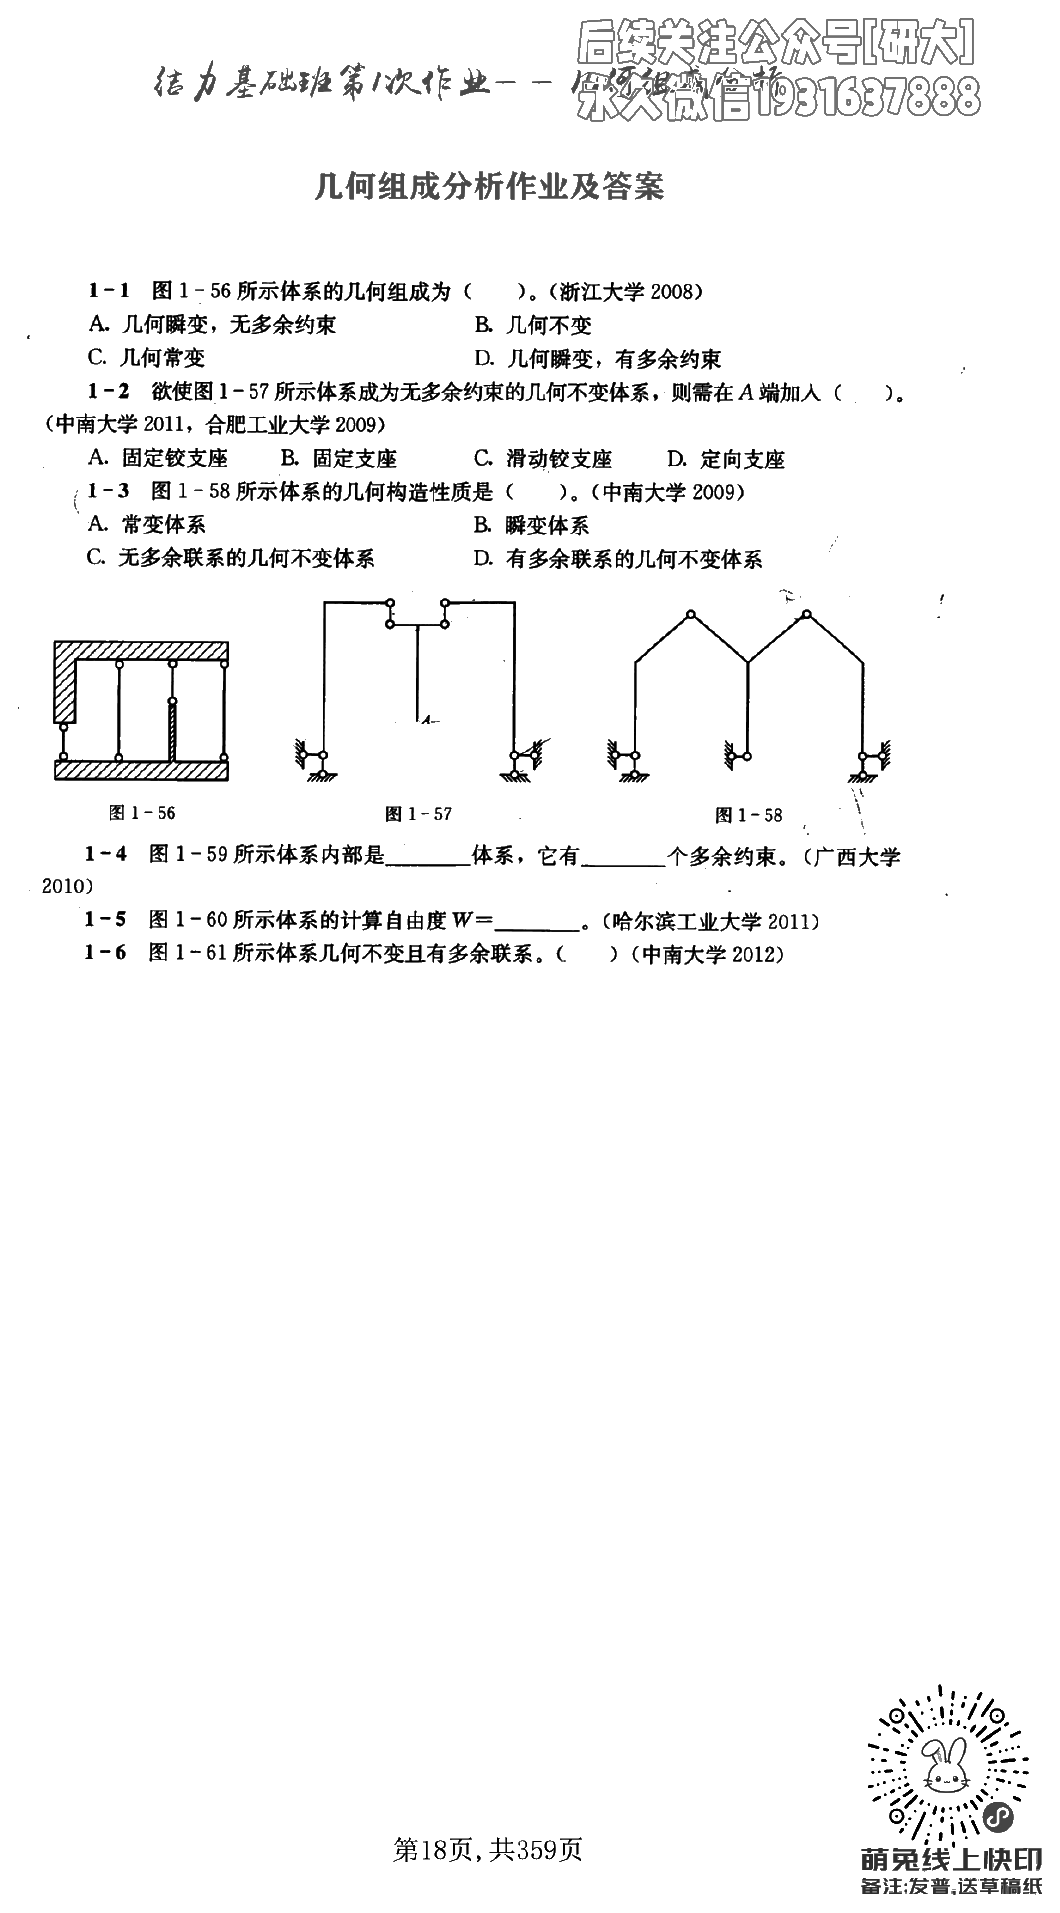
\includegraphics[width=0.96\textwidth,height=0.82\textheight,keepaspectratio]{images/c01_answer_2_p01.png}
\par\small 作业与答案（去水印版），第 7/9 页
\end{center}
\clearpage
\begin{center}
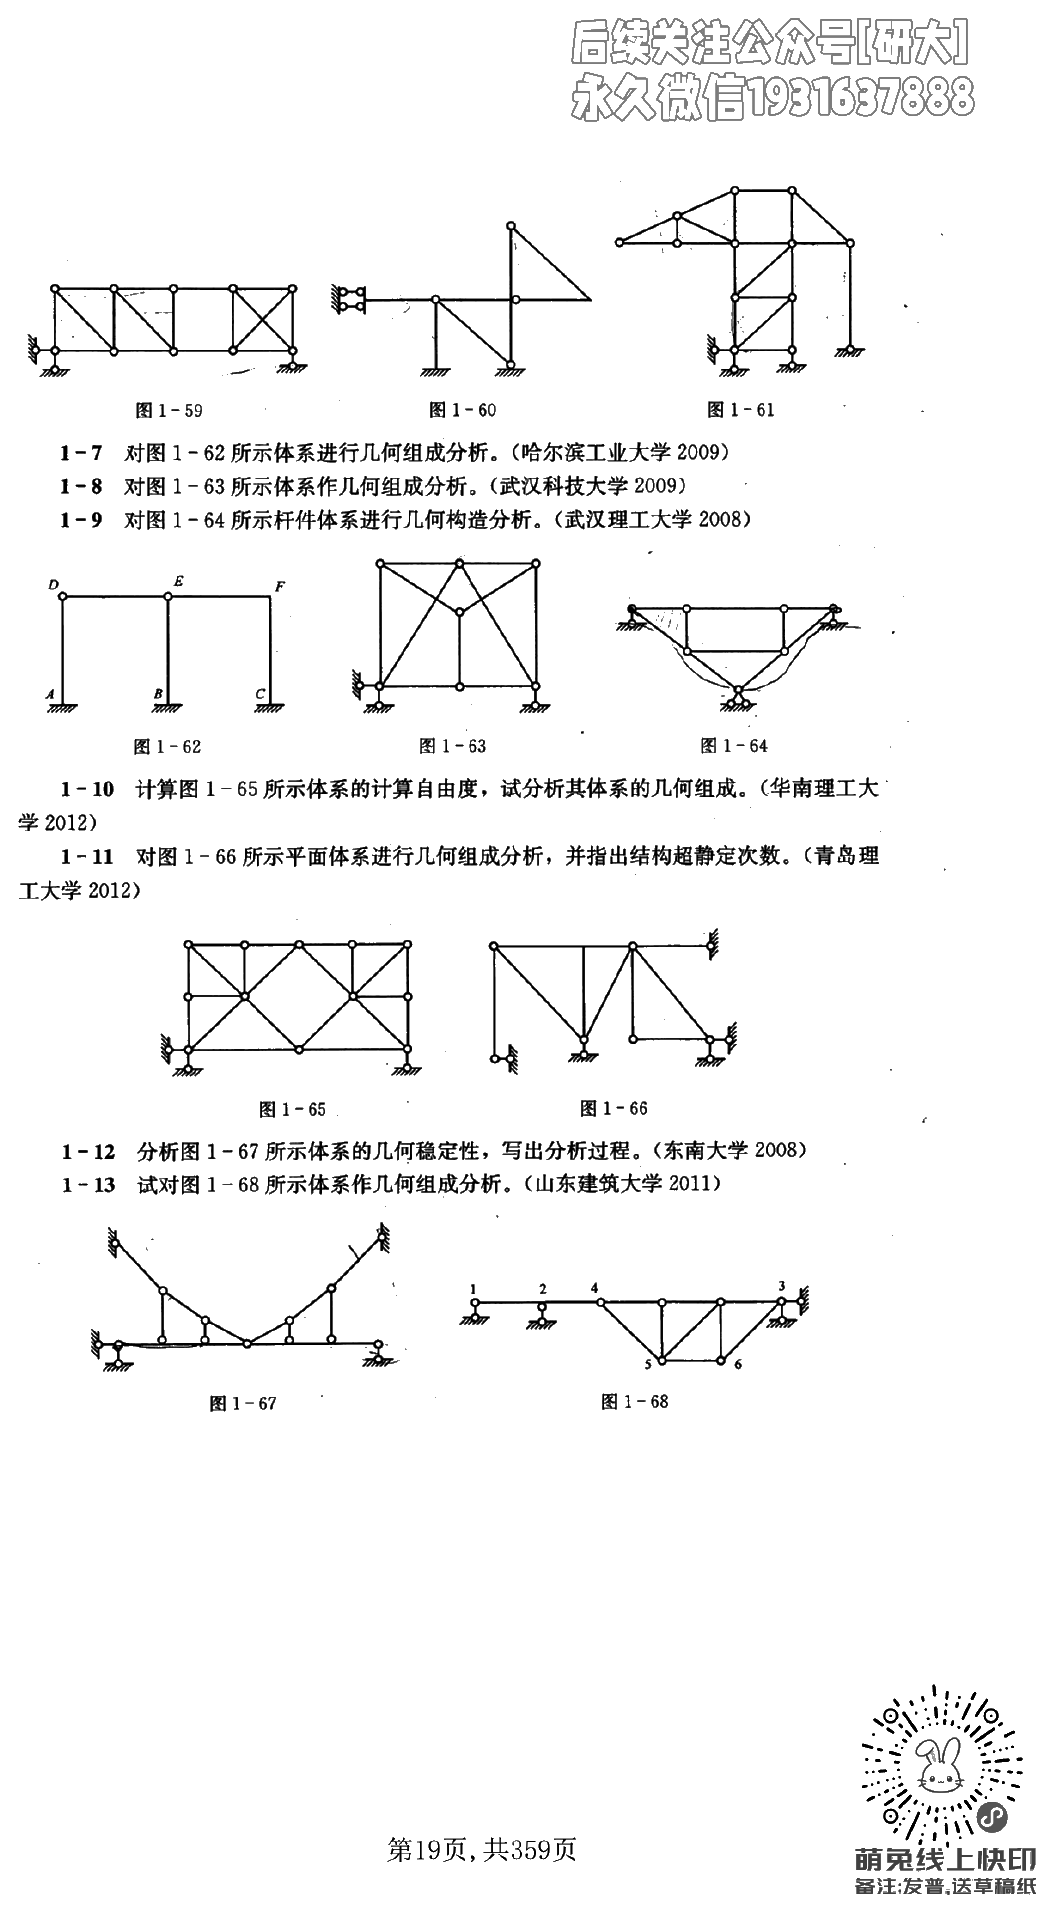
\includegraphics[width=0.96\textwidth,height=0.82\textheight,keepaspectratio]{images/c01_answer_2_p02.png}
\par\small 作业与答案（去水印版），第 8/9 页
\end{center}
\clearpage
\begin{center}
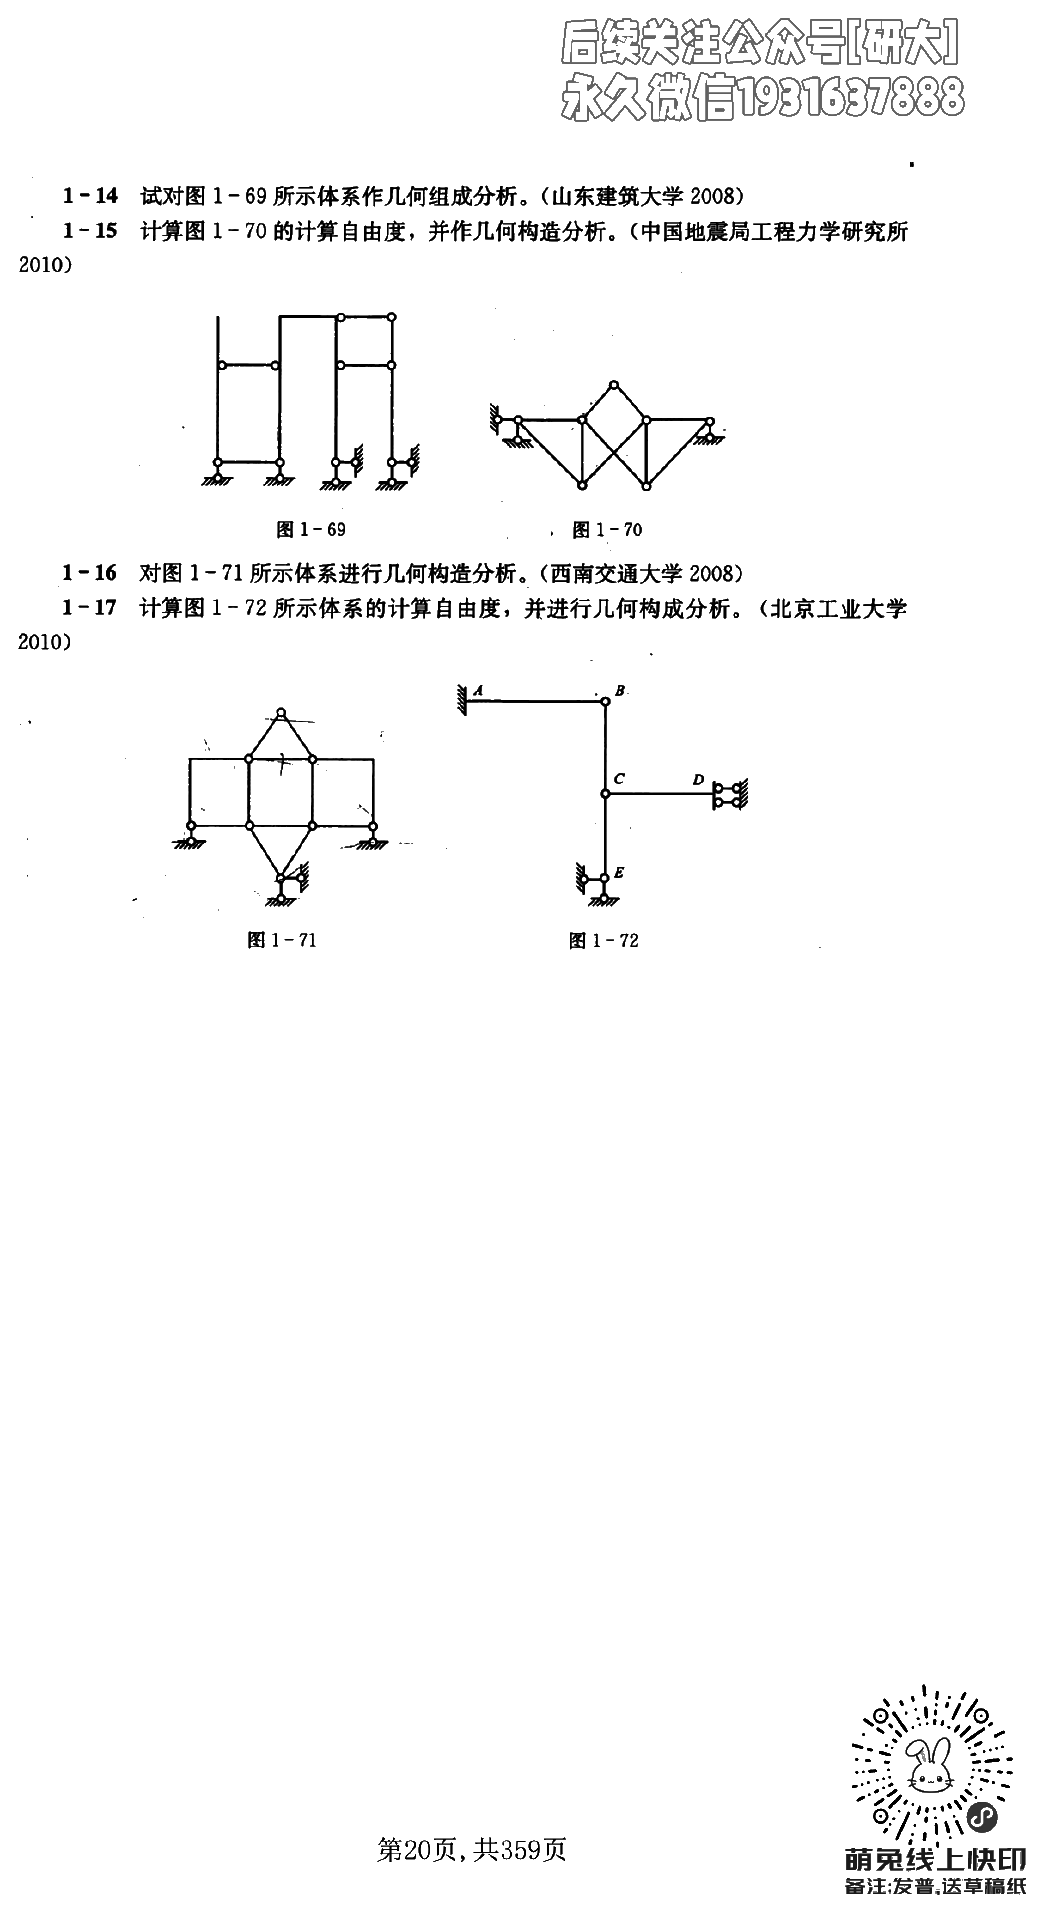
\includegraphics[width=0.96\textwidth,height=0.82\textheight,keepaspectratio]{images/c01_answer_2_p03.png}
\par\small 作业与答案（去水印版），第 9/9 页
\end{center}
\clearpage
\section{讲解笔记（去水印版）}
\begin{center}
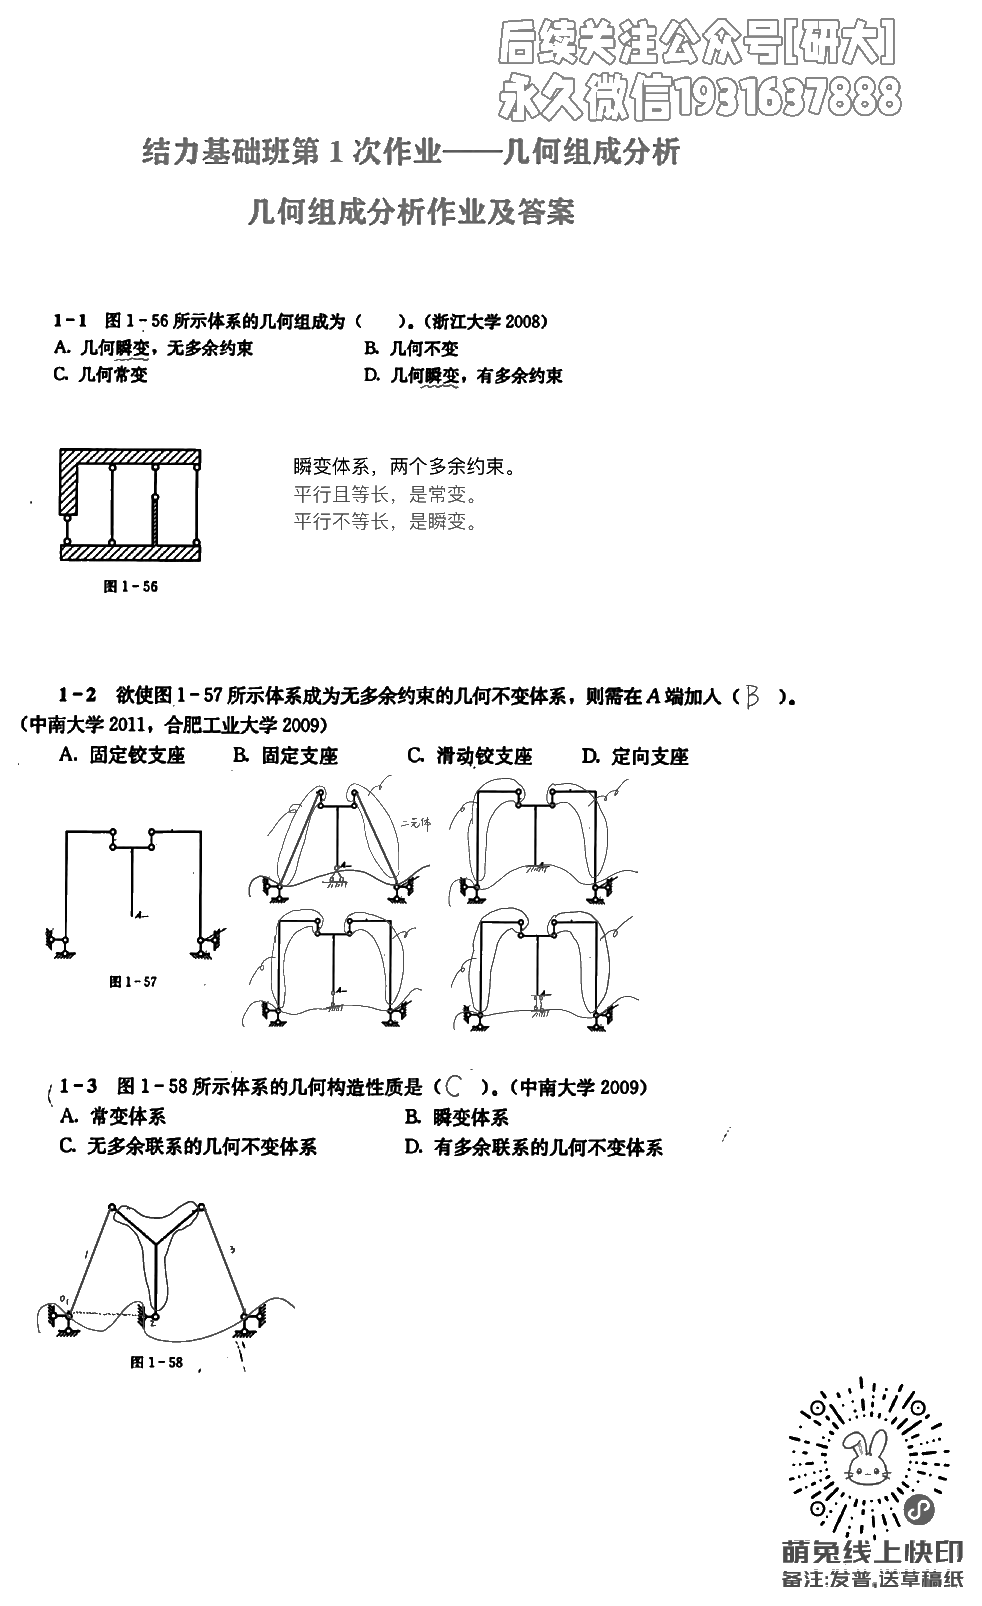
\includegraphics[width=0.96\textwidth,height=0.82\textheight,keepaspectratio]{images/c01_note_p01.png}
\par\small 讲解笔记（去水印版），第 1/6 页
\end{center}
\clearpage
\begin{center}
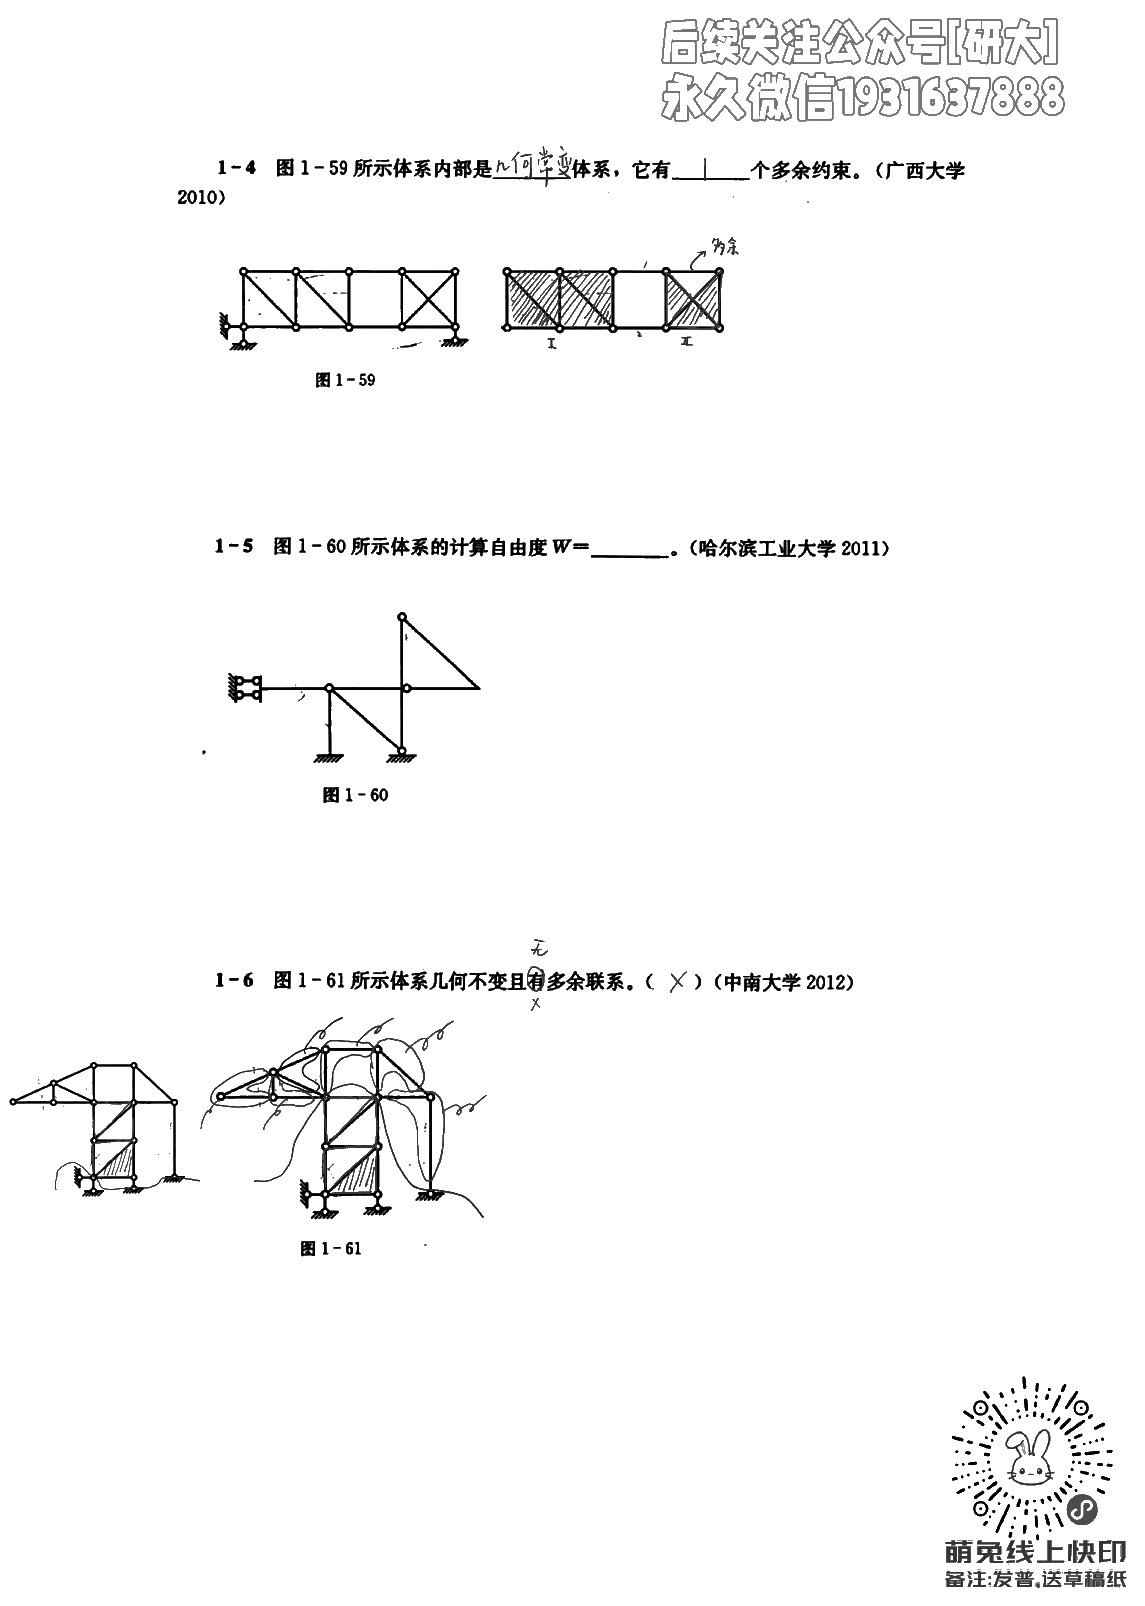
\includegraphics[width=0.96\textwidth,height=0.82\textheight,keepaspectratio]{images/c01_note_p02.png}
\par\small 讲解笔记（去水印版），第 2/6 页
\end{center}
\clearpage
\begin{center}
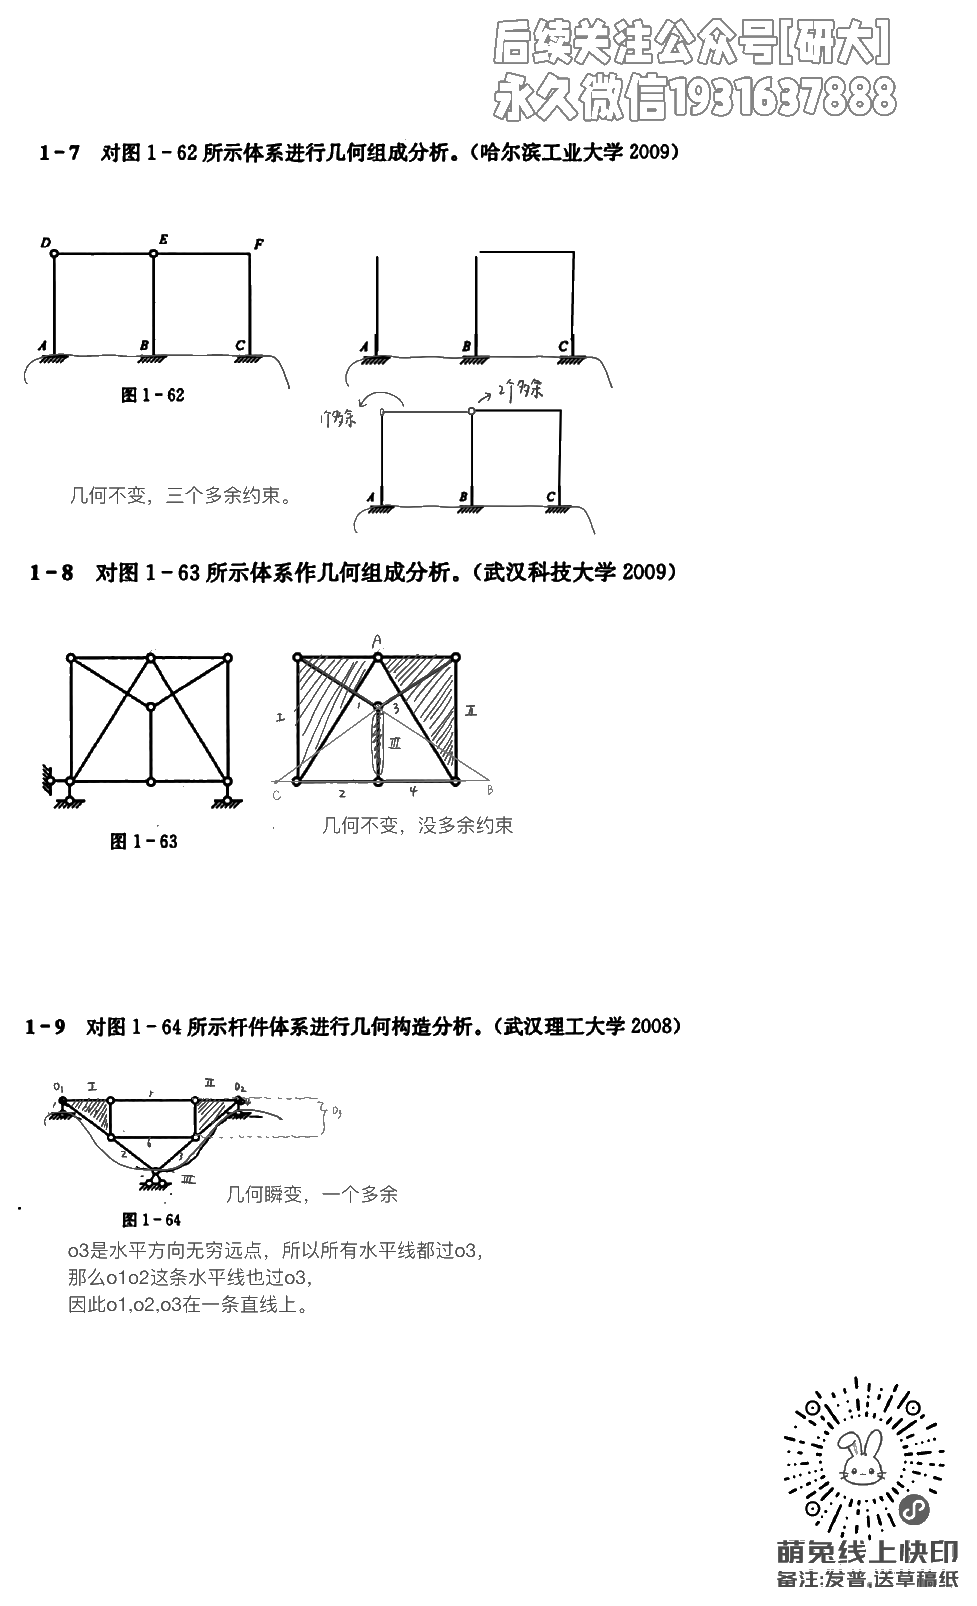
\includegraphics[width=0.96\textwidth,height=0.82\textheight,keepaspectratio]{images/c01_note_p03.png}
\par\small 讲解笔记（去水印版），第 3/6 页
\end{center}
\clearpage
\begin{center}
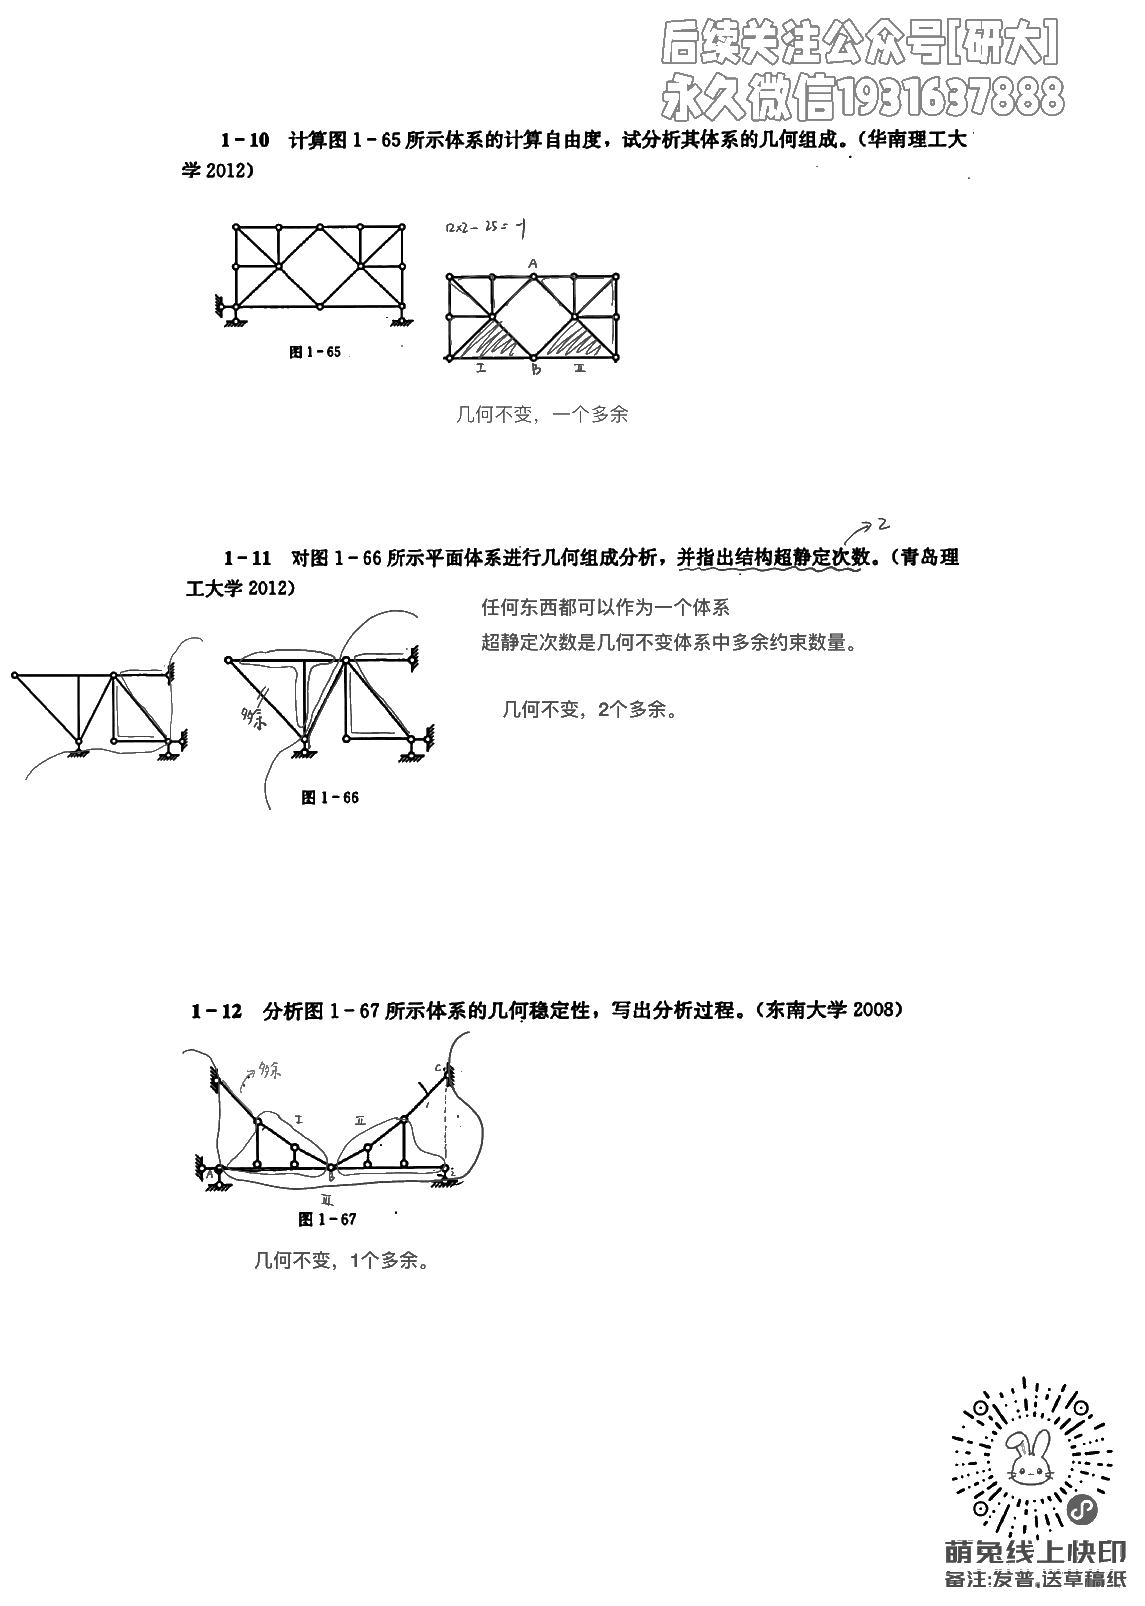
\includegraphics[width=0.96\textwidth,height=0.82\textheight,keepaspectratio]{images/c01_note_p04.png}
\par\small 讲解笔记（去水印版），第 4/6 页
\end{center}
\clearpage
\begin{center}
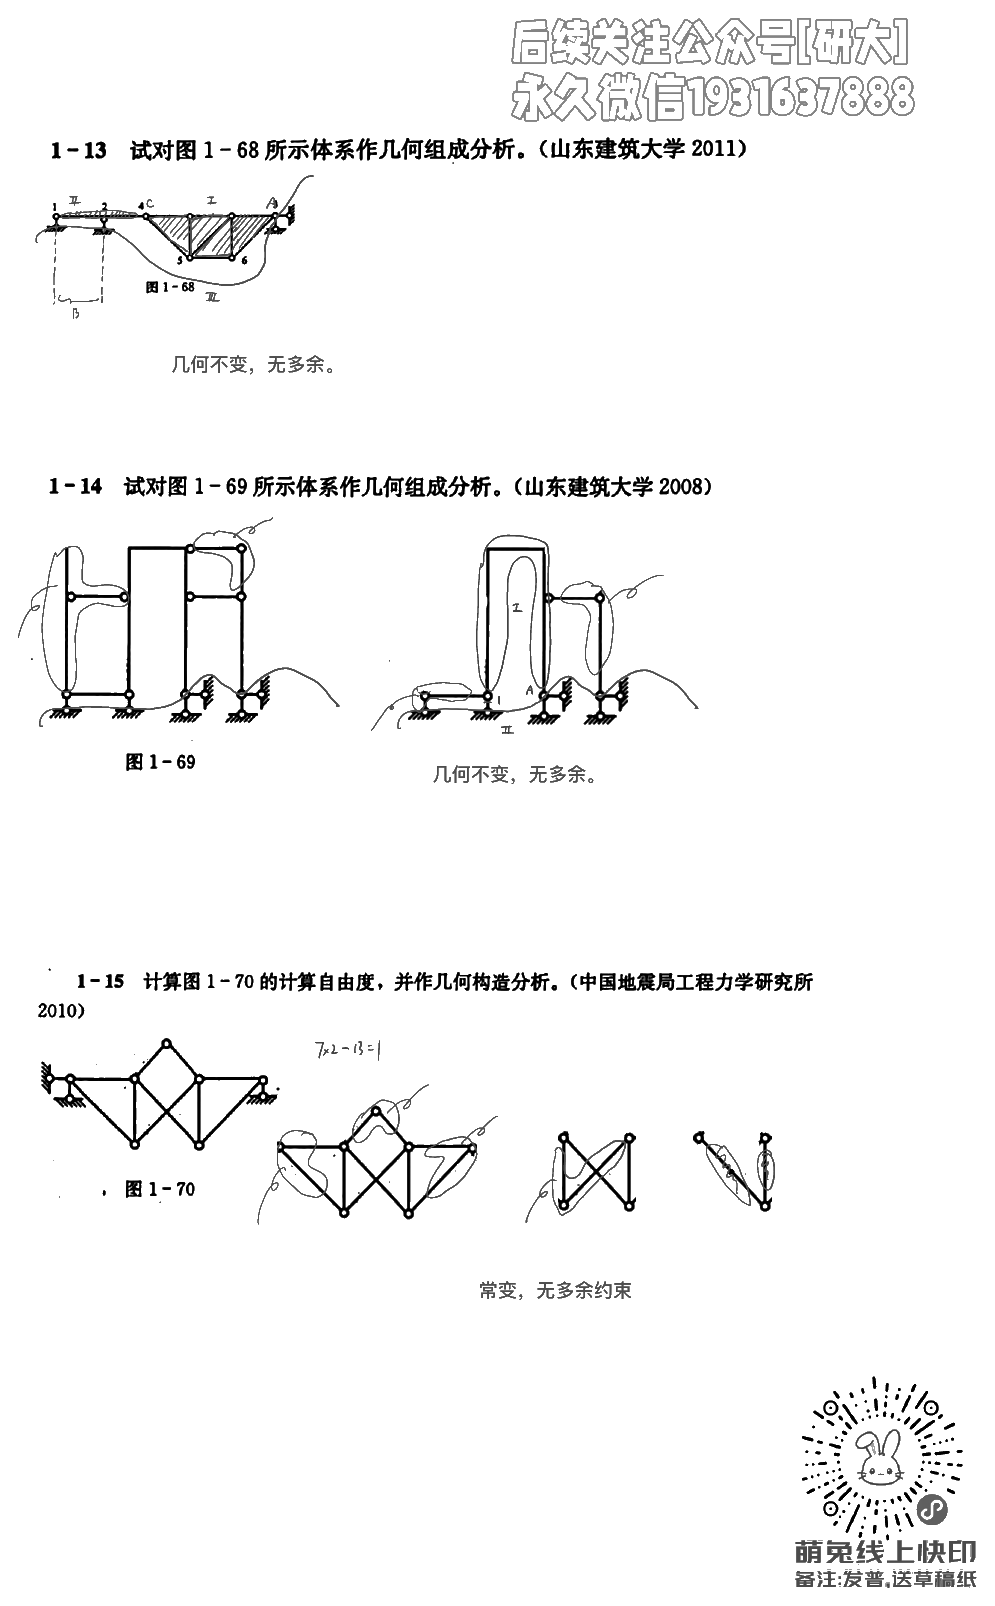
\includegraphics[width=0.96\textwidth,height=0.82\textheight,keepaspectratio]{images/c01_note_p05.png}
\par\small 讲解笔记（去水印版），第 5/6 页
\end{center}
\clearpage
\begin{center}
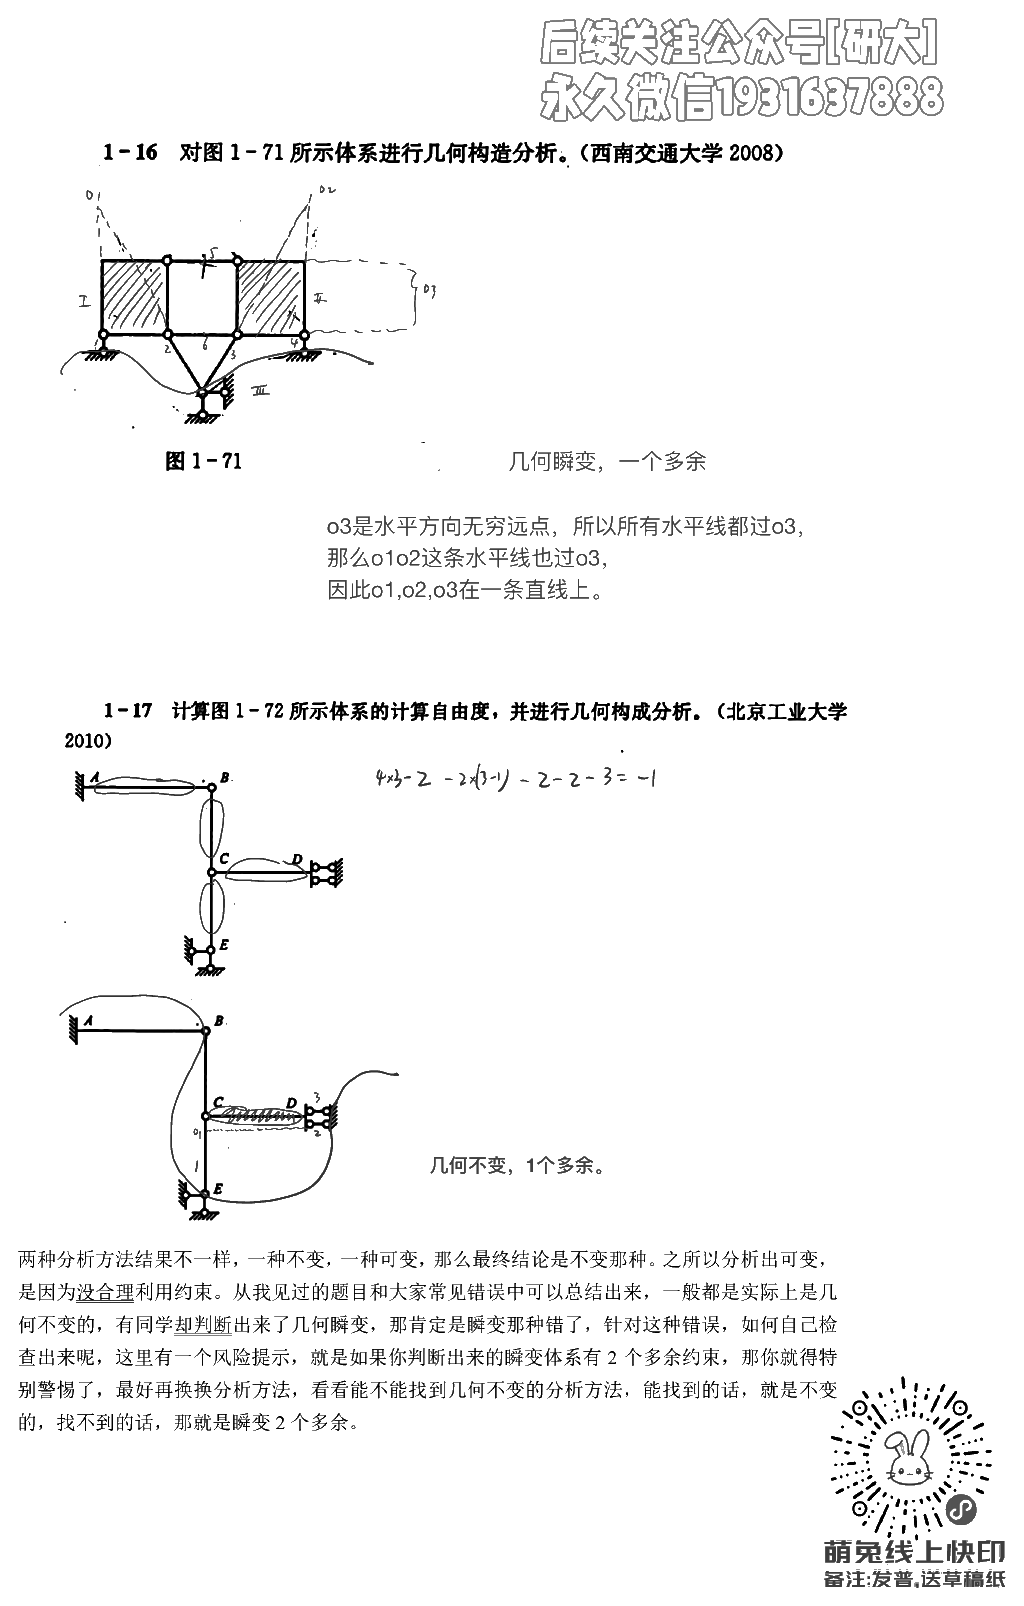
\includegraphics[width=0.96\textwidth,height=0.82\textheight,keepaspectratio]{images/c01_note_p06.png}
\par\small 讲解笔记（去水印版），第 6/6 页
\end{center}
\clearpage
\chapter{第2讲：理论力学回顾}
\begin{tcolorbox}[title=解析要点]
理论力学回顾的关键是受力图。先隔离研究对象，完整标注约束反力、集中力、分布力等，再列 $\sum F_x=0$、$\sum F_y=0$、$\sum M=0$ 求解。
\end{tcolorbox}
\begin{tcolorbox}[title=答案与校核]
答案页给出了各题平衡方程和反力结果；可用任一点力矩平衡复核。
\end{tcolorbox}
\section{作业与答案（去水印版）}
\begin{center}
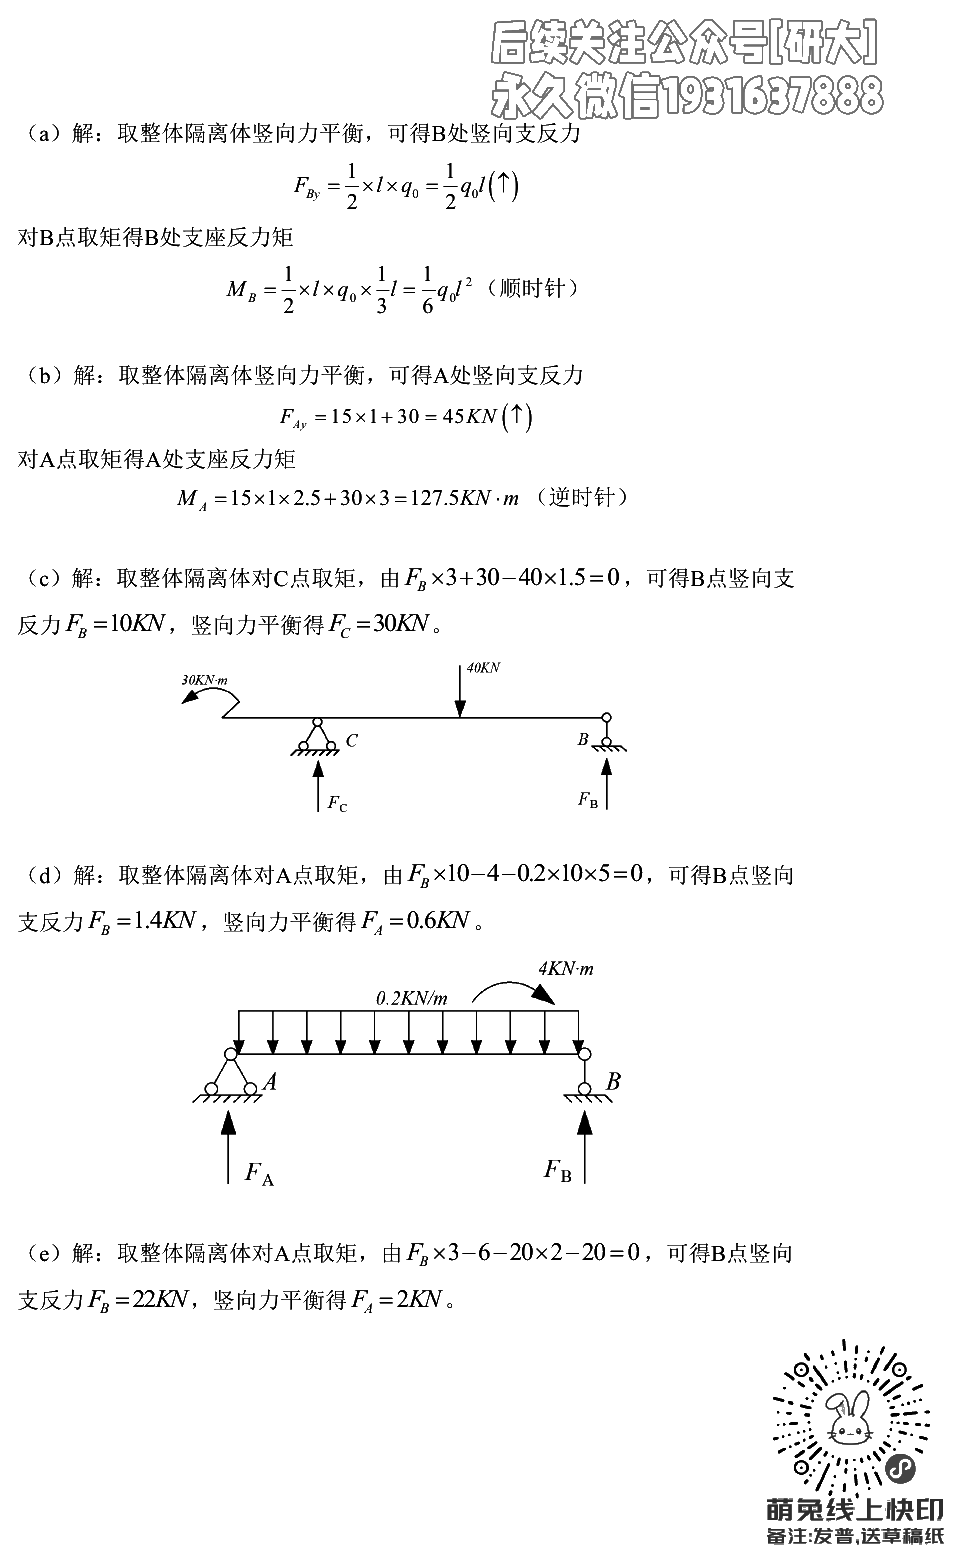
\includegraphics[width=0.96\textwidth,height=0.82\textheight,keepaspectratio]{images/c02_answer_1_p01.png}
\par\small 作业与答案（去水印版），第 1/6 页
\end{center}
\clearpage
\begin{center}
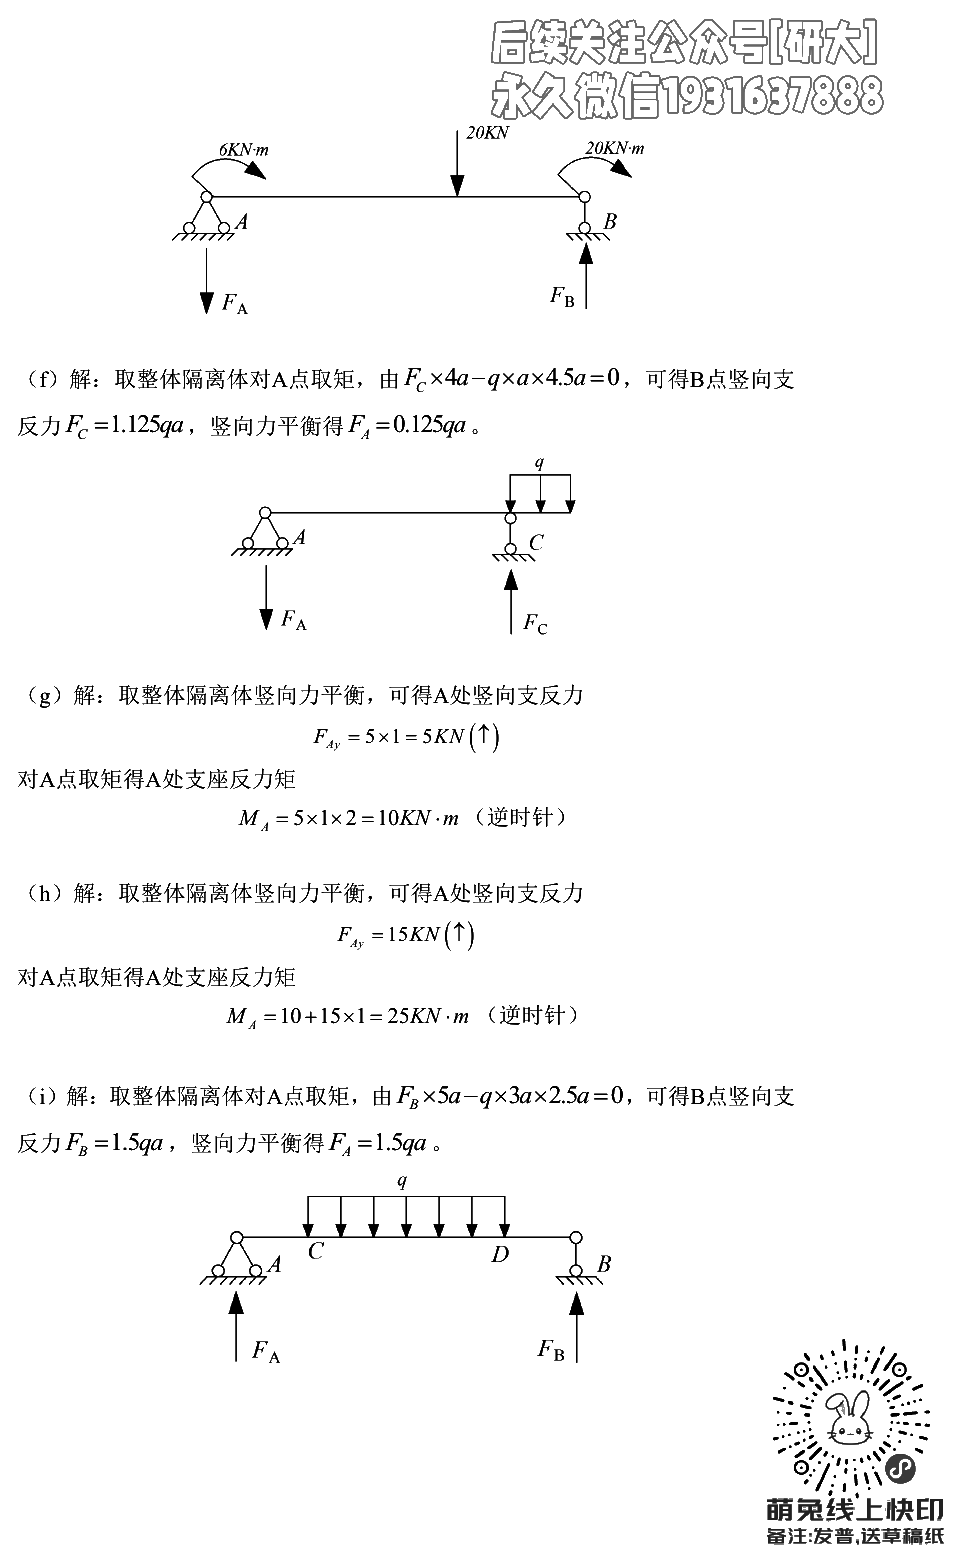
\includegraphics[width=0.96\textwidth,height=0.82\textheight,keepaspectratio]{images/c02_answer_1_p02.png}
\par\small 作业与答案（去水印版），第 2/6 页
\end{center}
\clearpage
\begin{center}
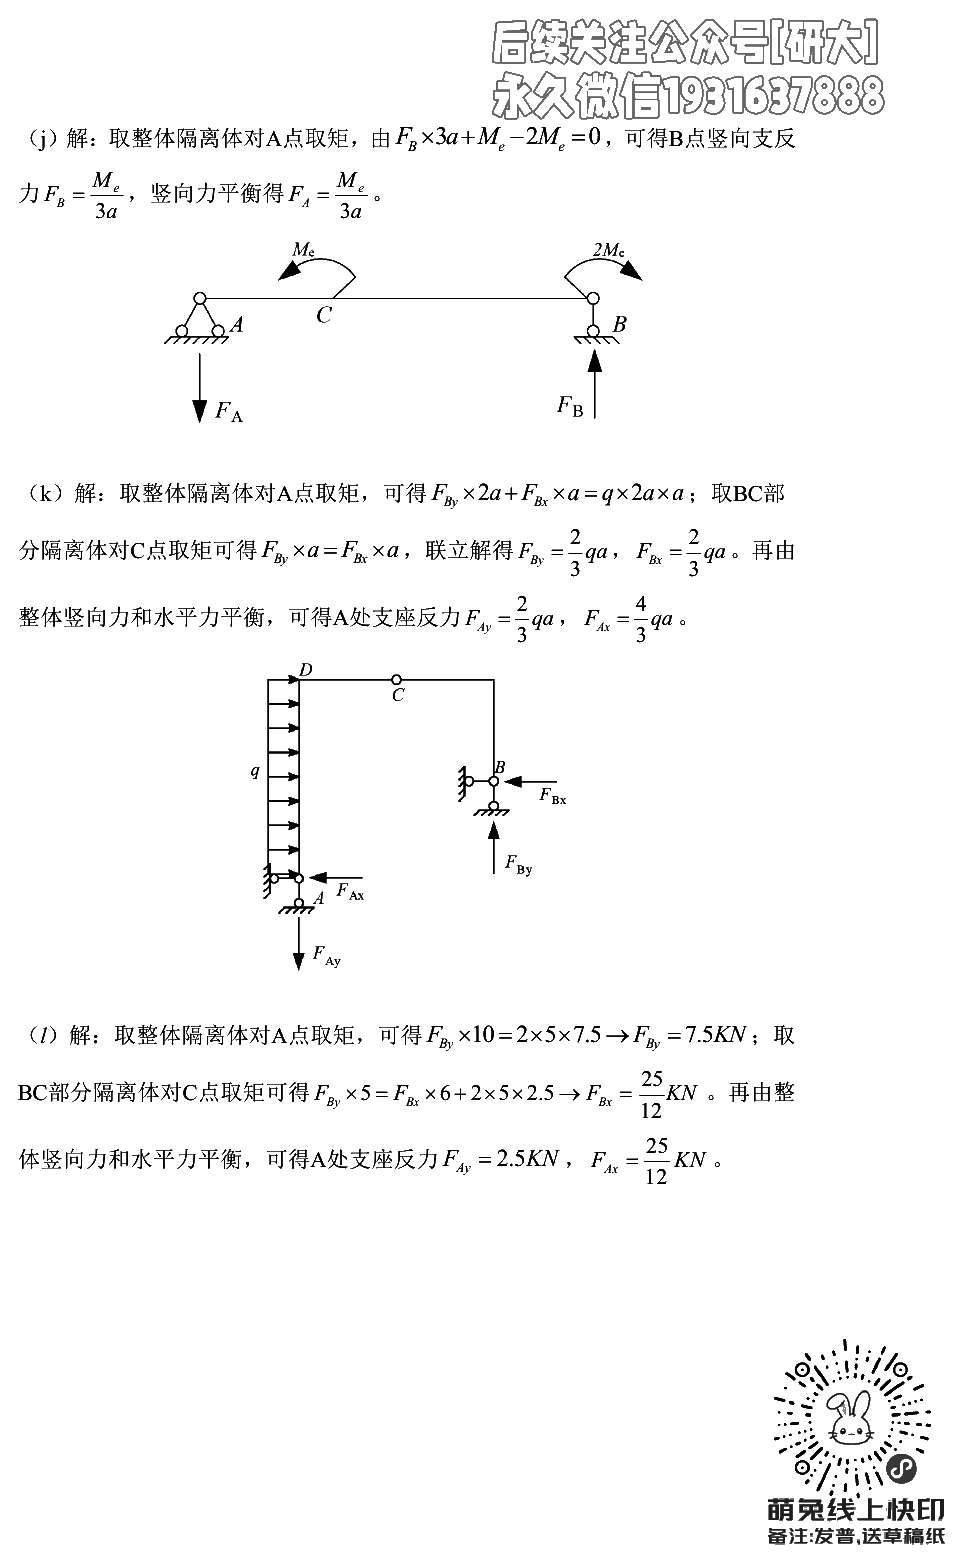
\includegraphics[width=0.96\textwidth,height=0.82\textheight,keepaspectratio]{images/c02_answer_1_p03.png}
\par\small 作业与答案（去水印版），第 3/6 页
\end{center}
\clearpage
\begin{center}
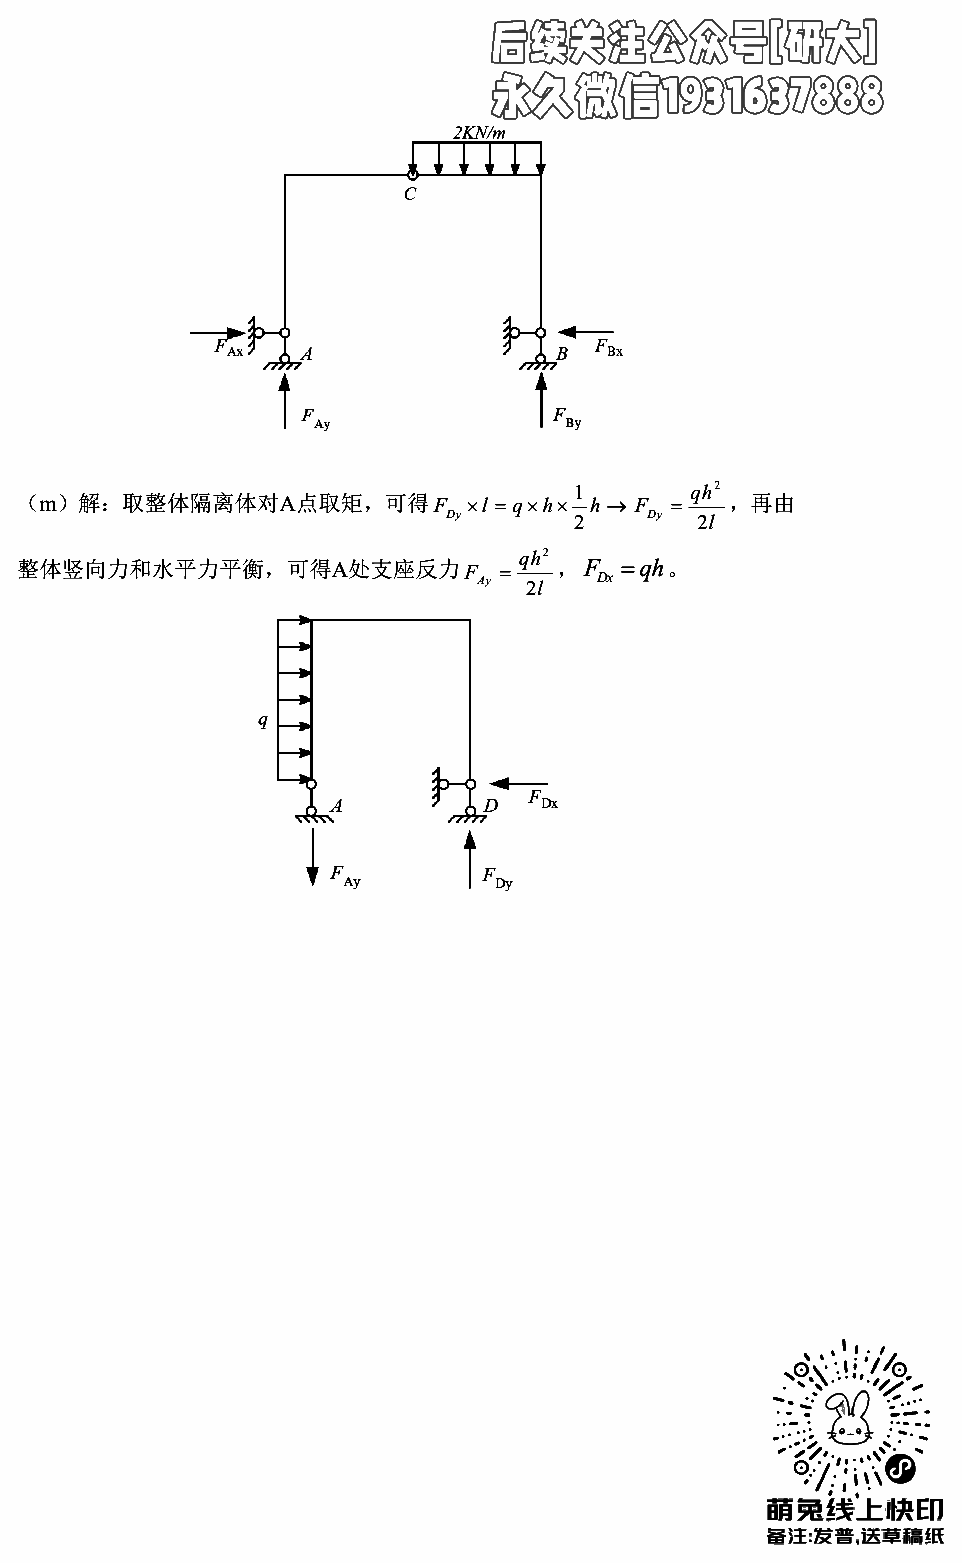
\includegraphics[width=0.96\textwidth,height=0.82\textheight,keepaspectratio]{images/c02_answer_1_p04.png}
\par\small 作业与答案（去水印版），第 4/6 页
\end{center}
\clearpage
\begin{center}
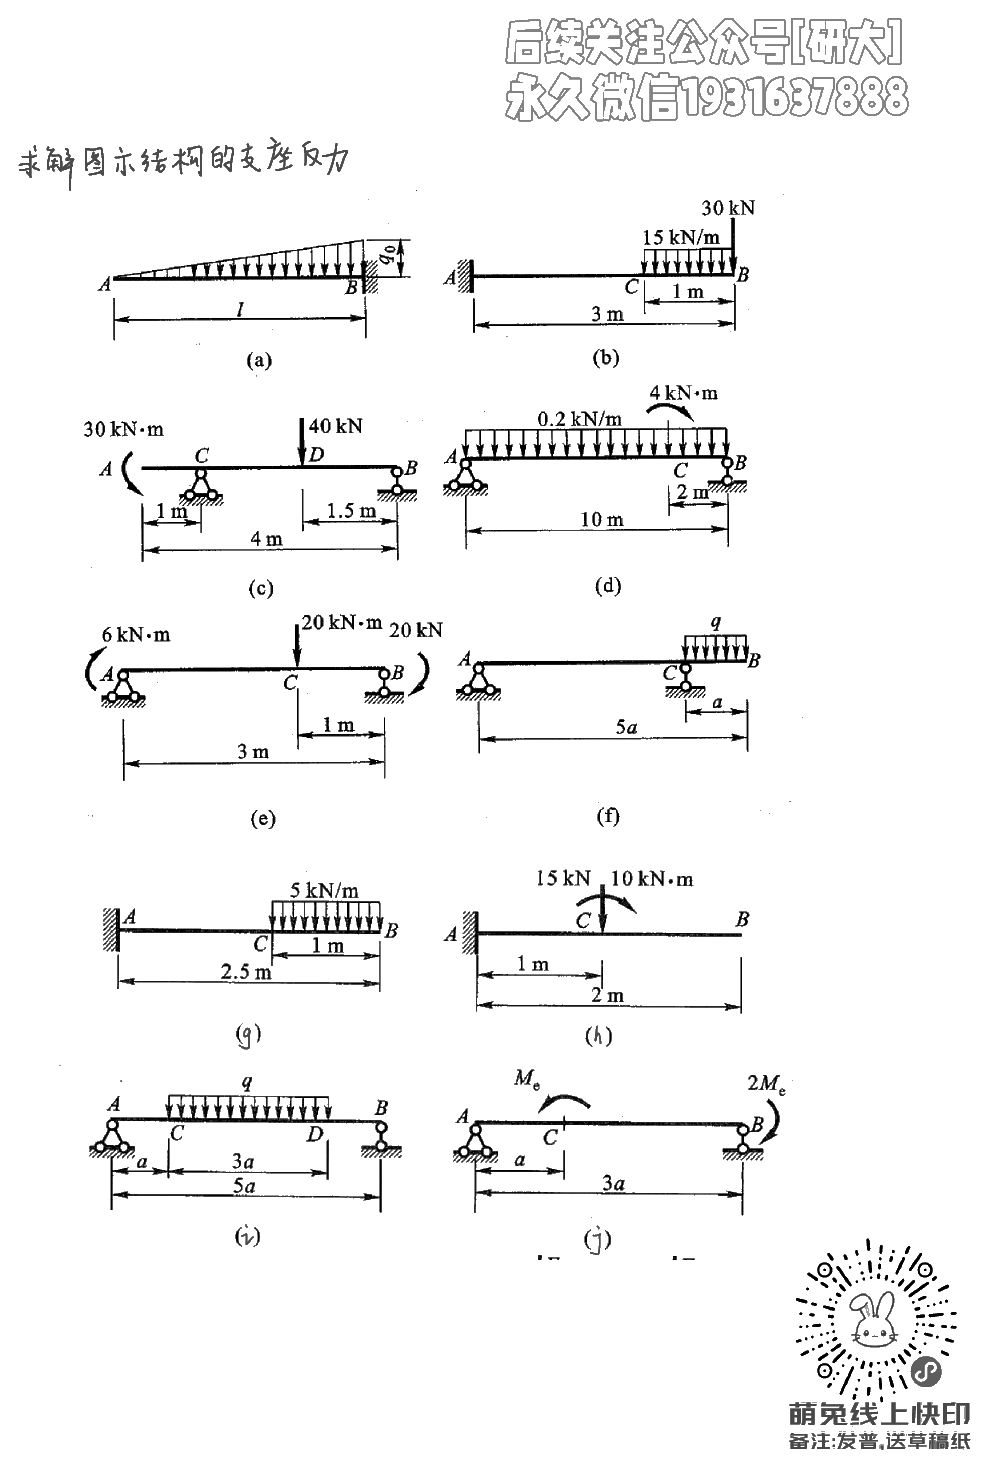
\includegraphics[width=0.96\textwidth,height=0.82\textheight,keepaspectratio]{images/c02_answer_2_p01.png}
\par\small 作业与答案（去水印版），第 5/6 页
\end{center}
\clearpage
\begin{center}
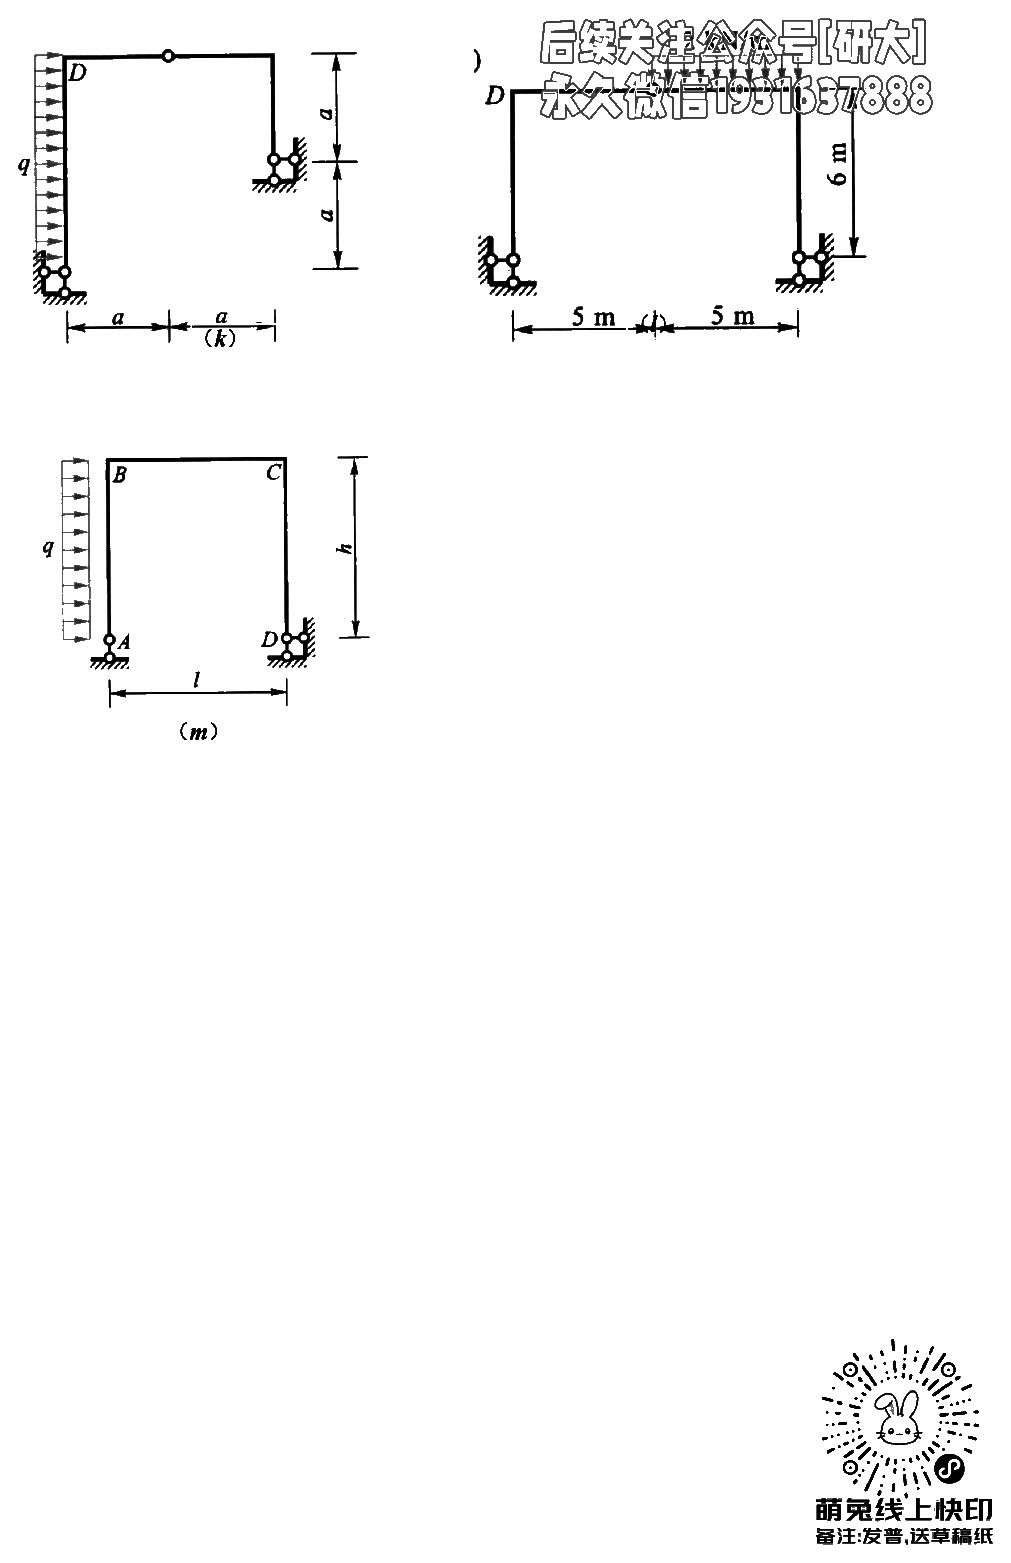
\includegraphics[width=0.96\textwidth,height=0.82\textheight,keepaspectratio]{images/c02_answer_2_p02.png}
\par\small 作业与答案（去水印版），第 6/6 页
\end{center}
\clearpage
\section{讲解笔记（去水印版）}
\begin{center}
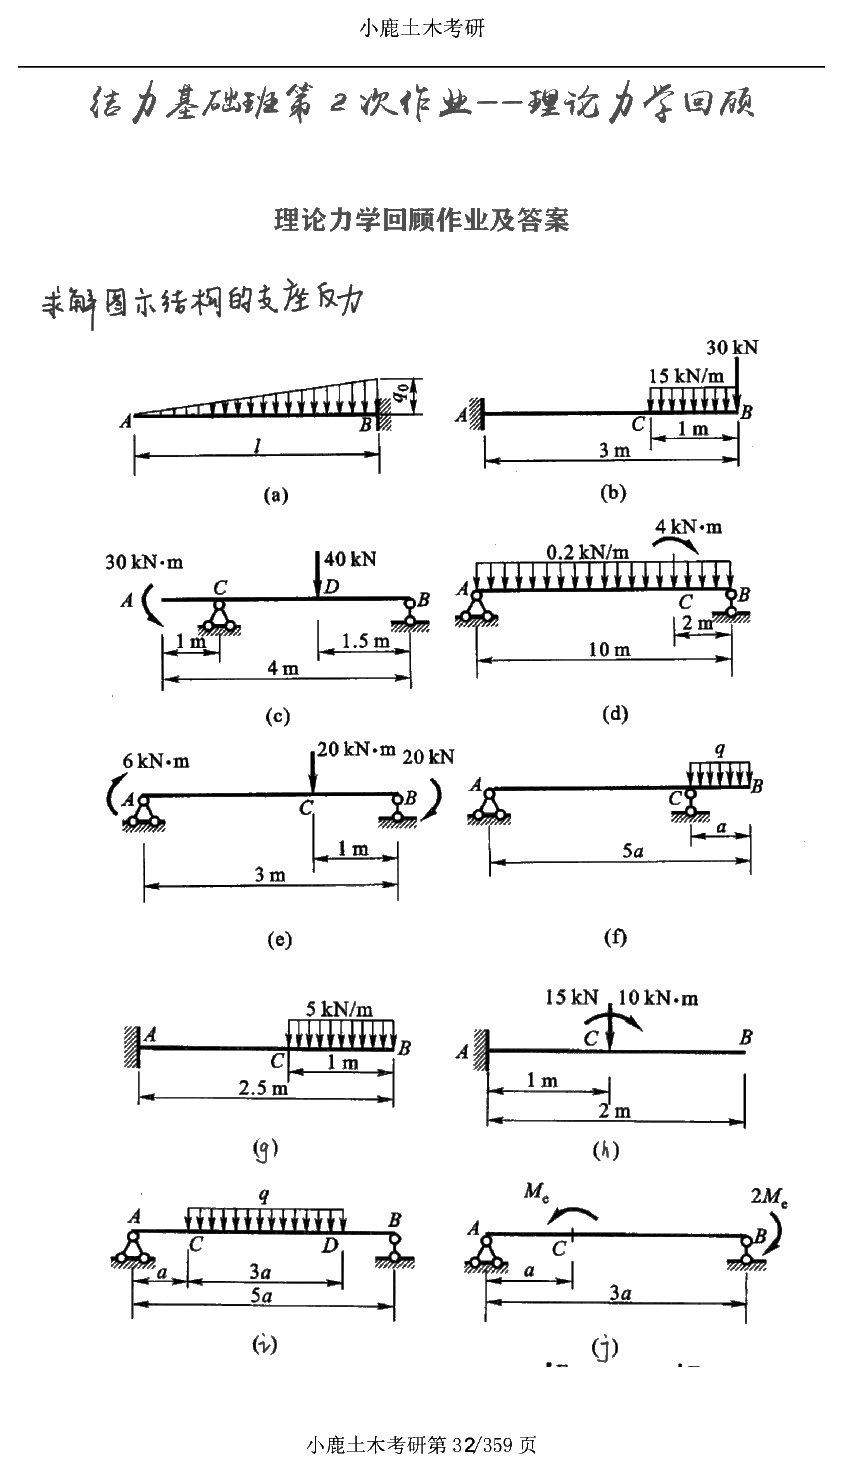
\includegraphics[width=0.96\textwidth,height=0.82\textheight,keepaspectratio]{images/c02_note_p01.png}
\par\small 讲解笔记（去水印版），第 1/4 页
\end{center}
\clearpage
\begin{center}
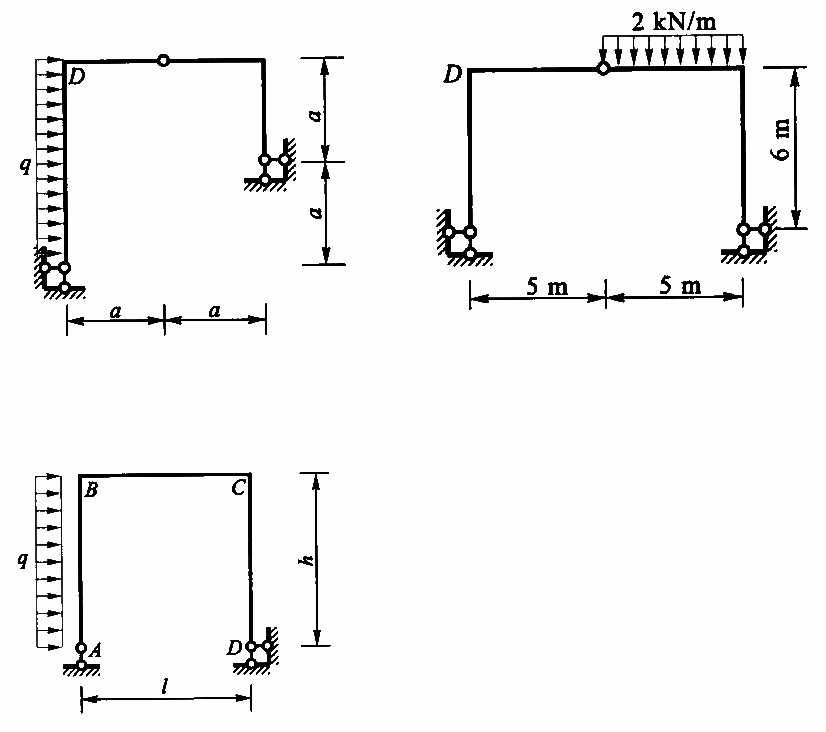
\includegraphics[width=0.96\textwidth,height=0.82\textheight,keepaspectratio]{images/c02_note_p02.png}
\par\small 讲解笔记（去水印版），第 2/4 页
\end{center}
\clearpage
\begin{center}
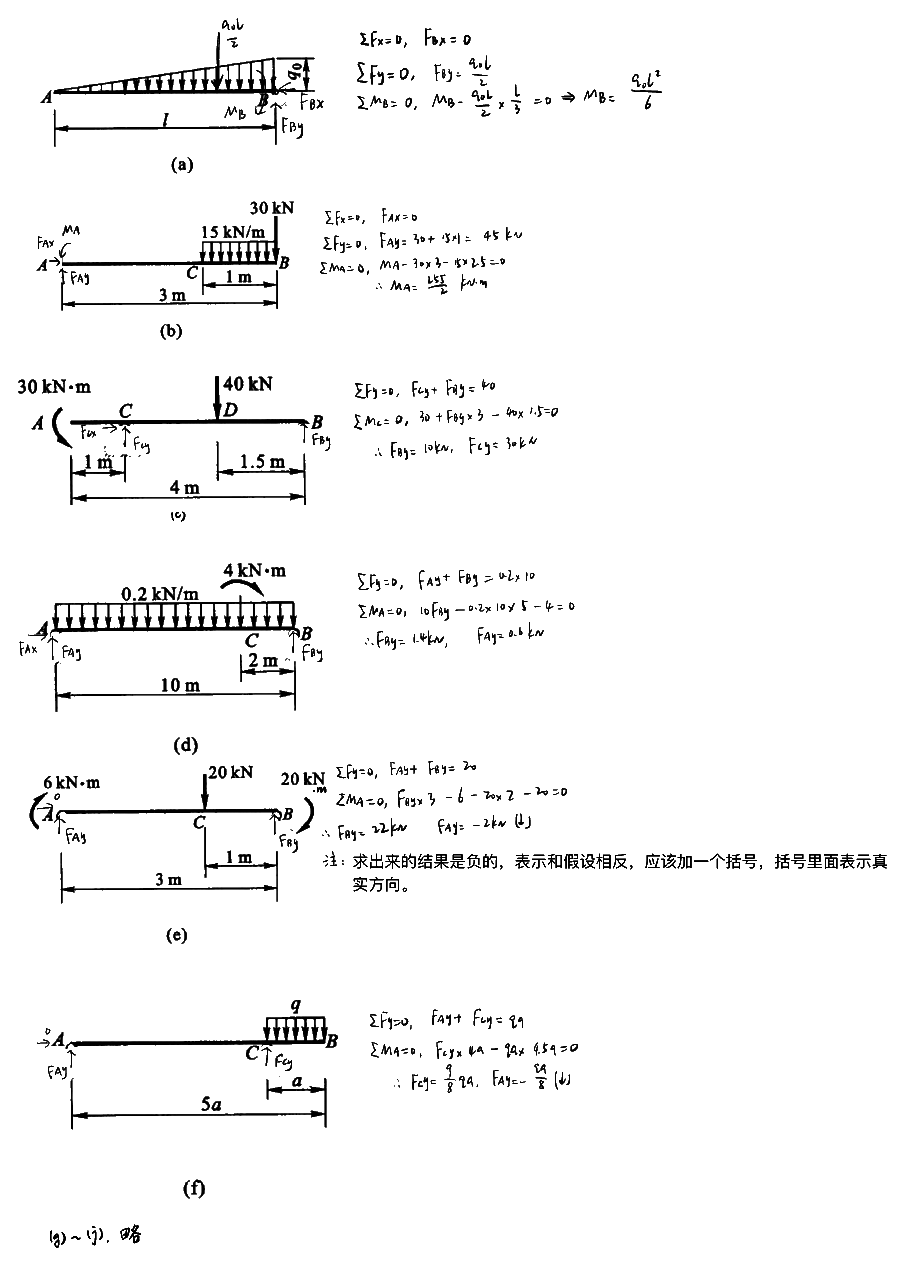
\includegraphics[width=0.96\textwidth,height=0.82\textheight,keepaspectratio]{images/c02_note_p03.png}
\par\small 讲解笔记（去水印版），第 3/4 页
\end{center}
\clearpage
\begin{center}
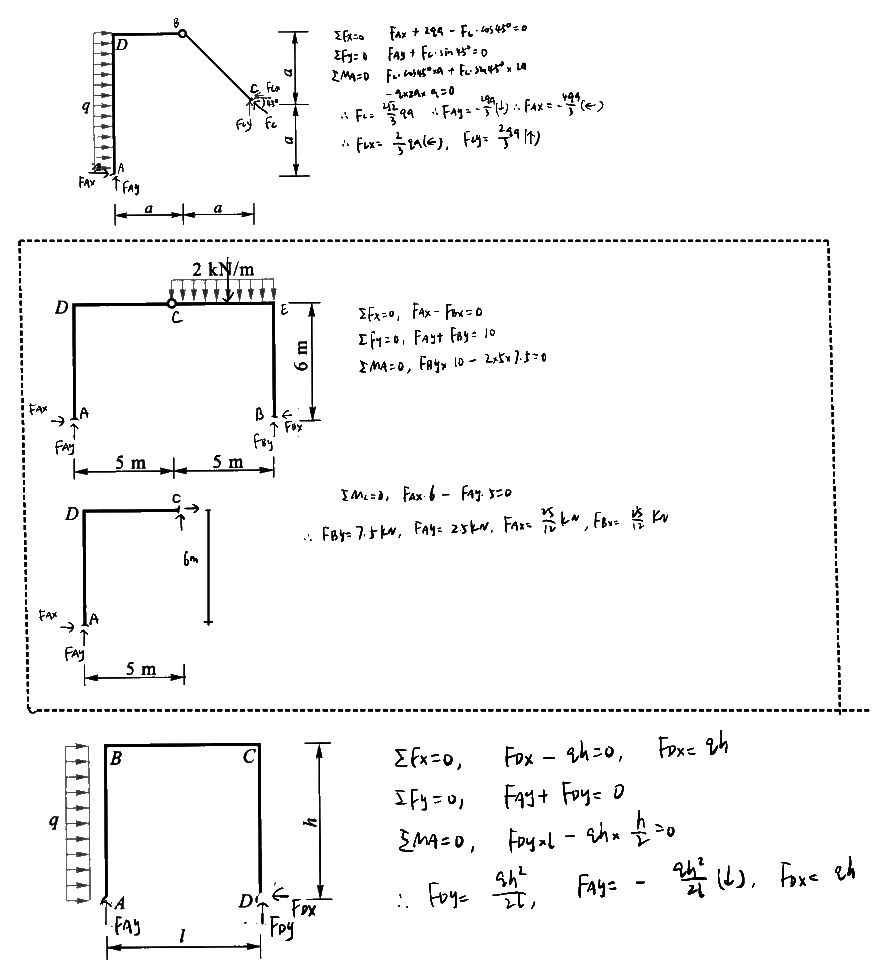
\includegraphics[width=0.96\textwidth,height=0.82\textheight,keepaspectratio]{images/c02_note_p04.png}
\par\small 讲解笔记（去水印版），第 4/4 页
\end{center}
\clearpage
\chapter{第3讲：材料力学回顾}
\begin{tcolorbox}[title=解析要点]
材料力学题通常按“内力—应力—变形—强度/刚度校核”组织。弯曲问题要注意截面惯性矩、正负号和最大应力位置。
\end{tcolorbox}
\begin{tcolorbox}[title=答案与校核]
答案页包含材料力学回顾题的计算过程；重点核对截面内力、应力公式和变形公式。
\end{tcolorbox}
\section{作业与答案（去水印版）}
\begin{center}
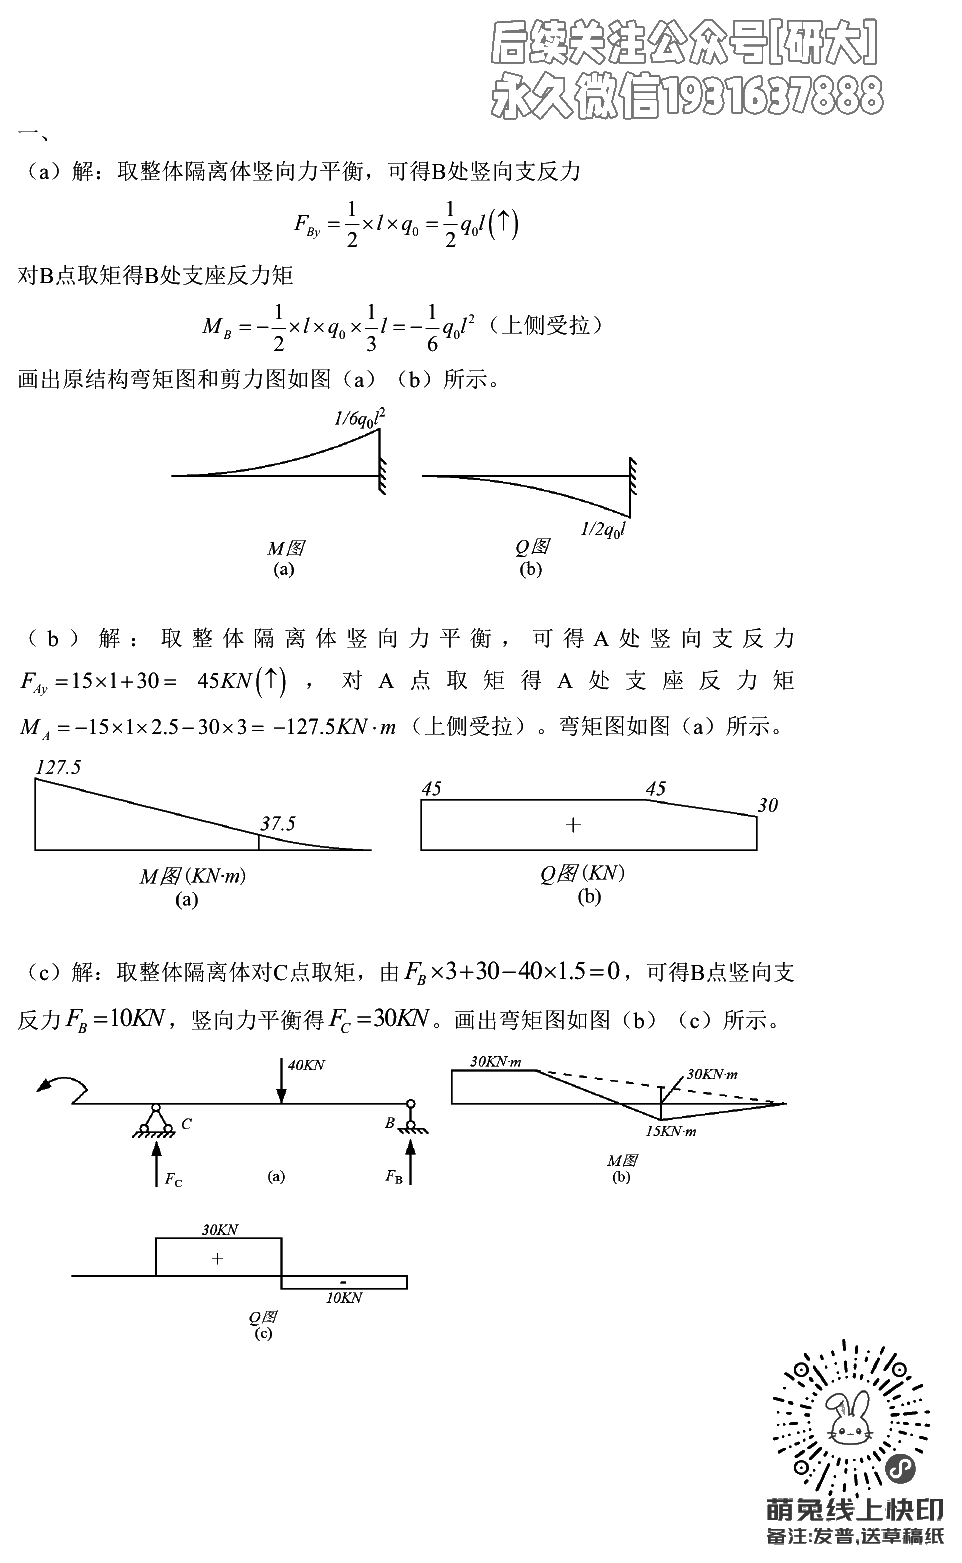
\includegraphics[width=0.96\textwidth,height=0.82\textheight,keepaspectratio]{images/c03_answer_1_p01.png}
\par\small 作业与答案（去水印版），第 1/19 页
\end{center}
\clearpage
\begin{center}
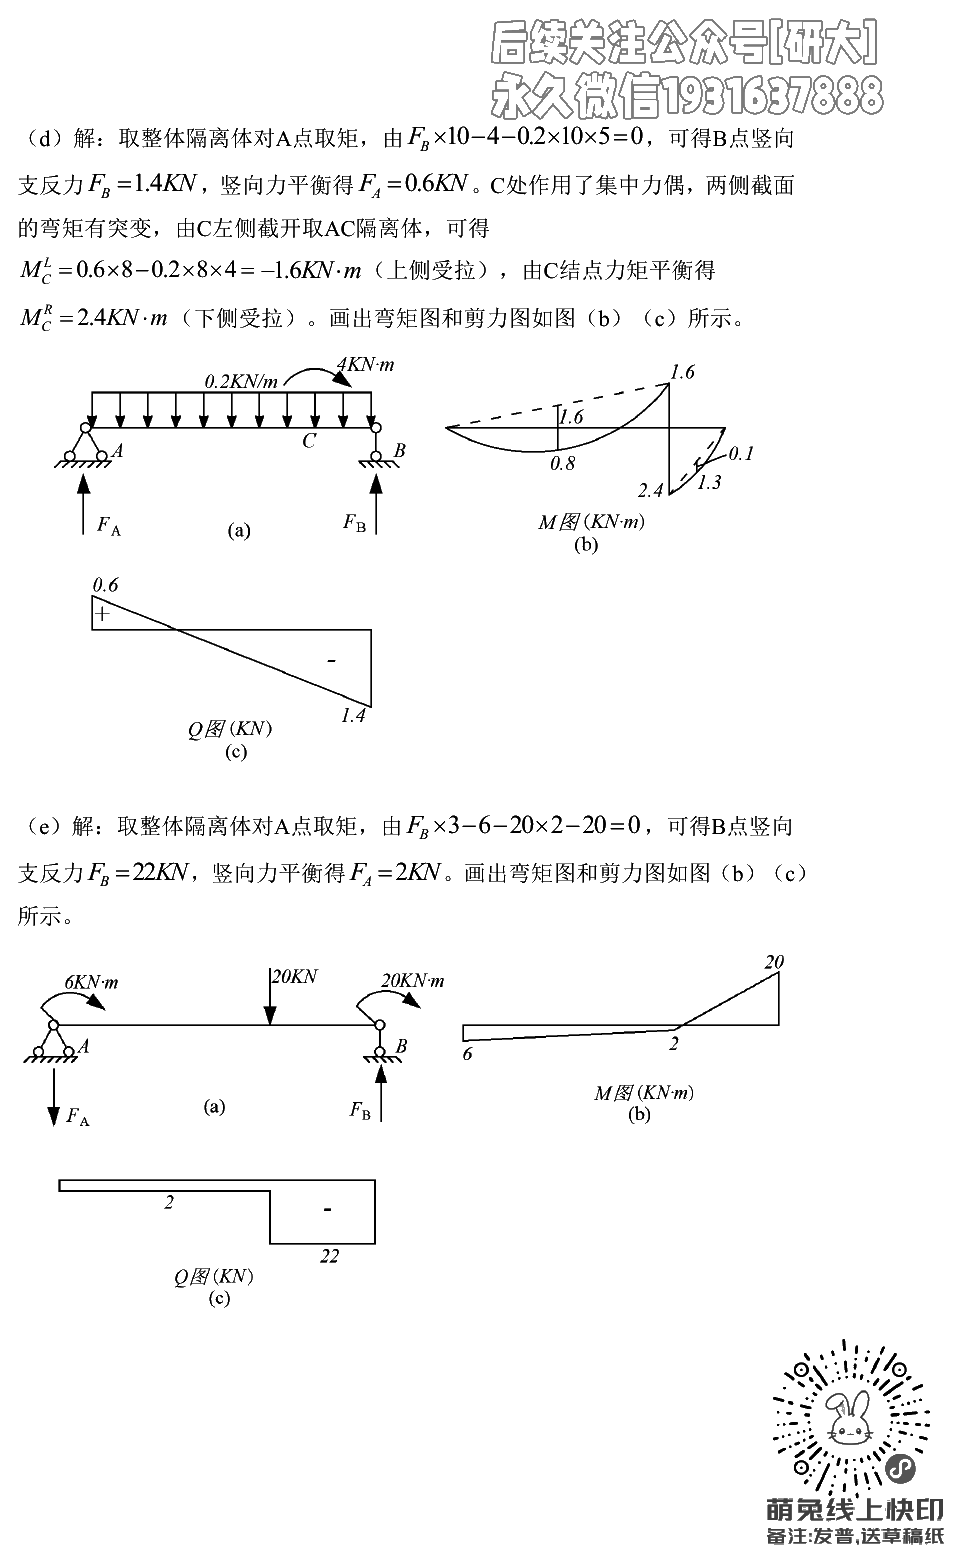
\includegraphics[width=0.96\textwidth,height=0.82\textheight,keepaspectratio]{images/c03_answer_1_p02.png}
\par\small 作业与答案（去水印版），第 2/19 页
\end{center}
\clearpage
\begin{center}
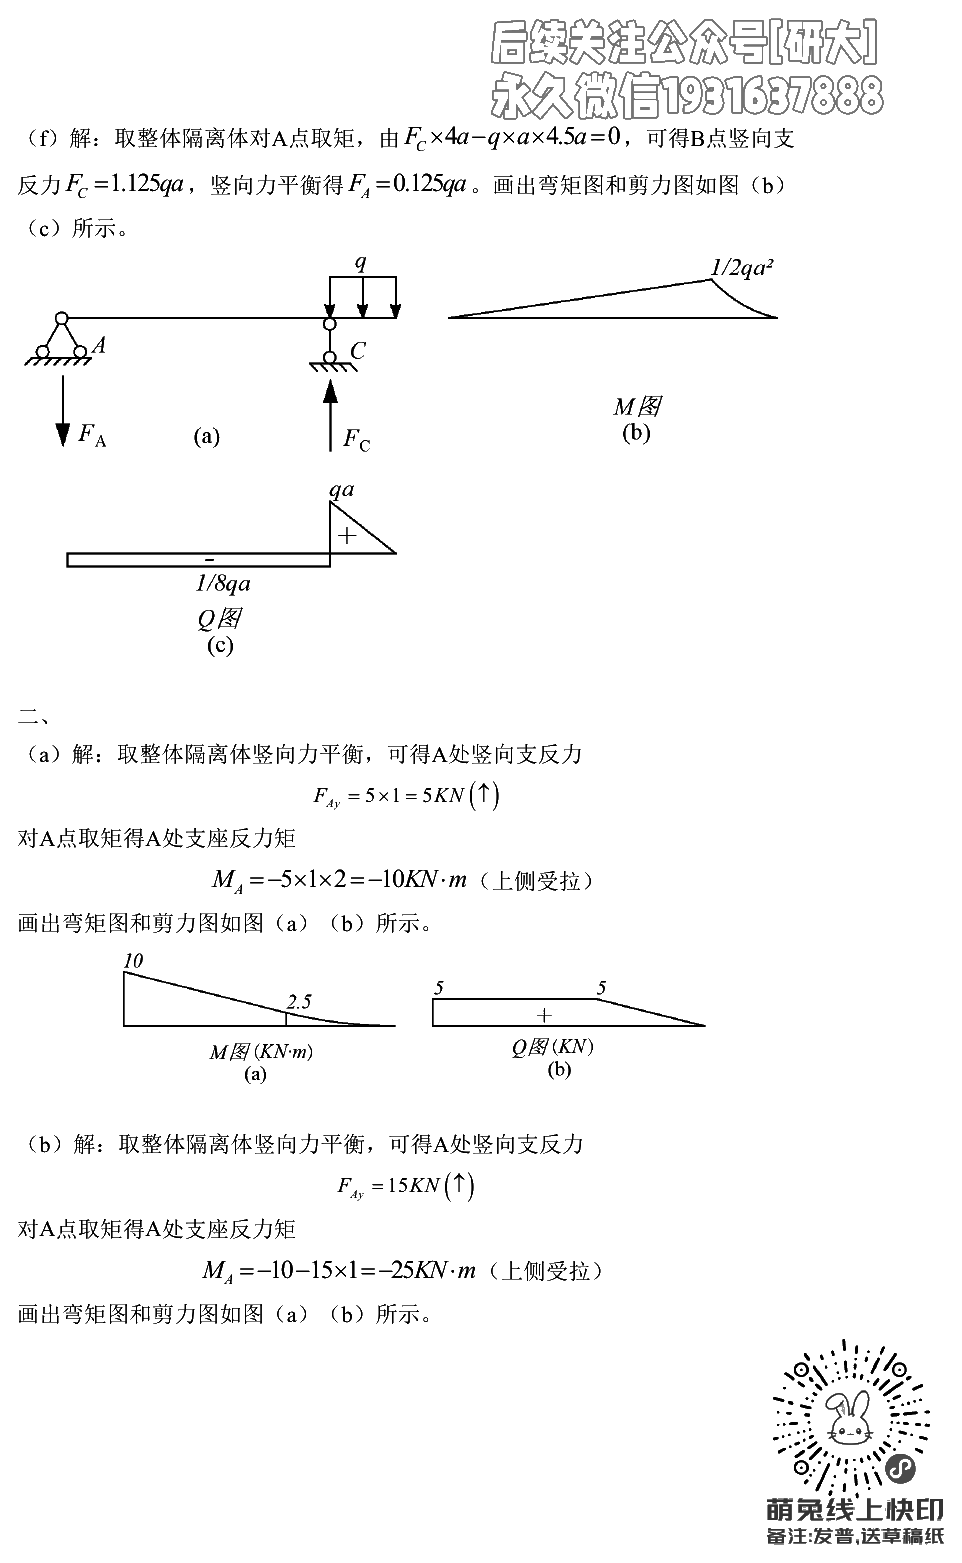
\includegraphics[width=0.96\textwidth,height=0.82\textheight,keepaspectratio]{images/c03_answer_1_p03.png}
\par\small 作业与答案（去水印版），第 3/19 页
\end{center}
\clearpage
\begin{center}
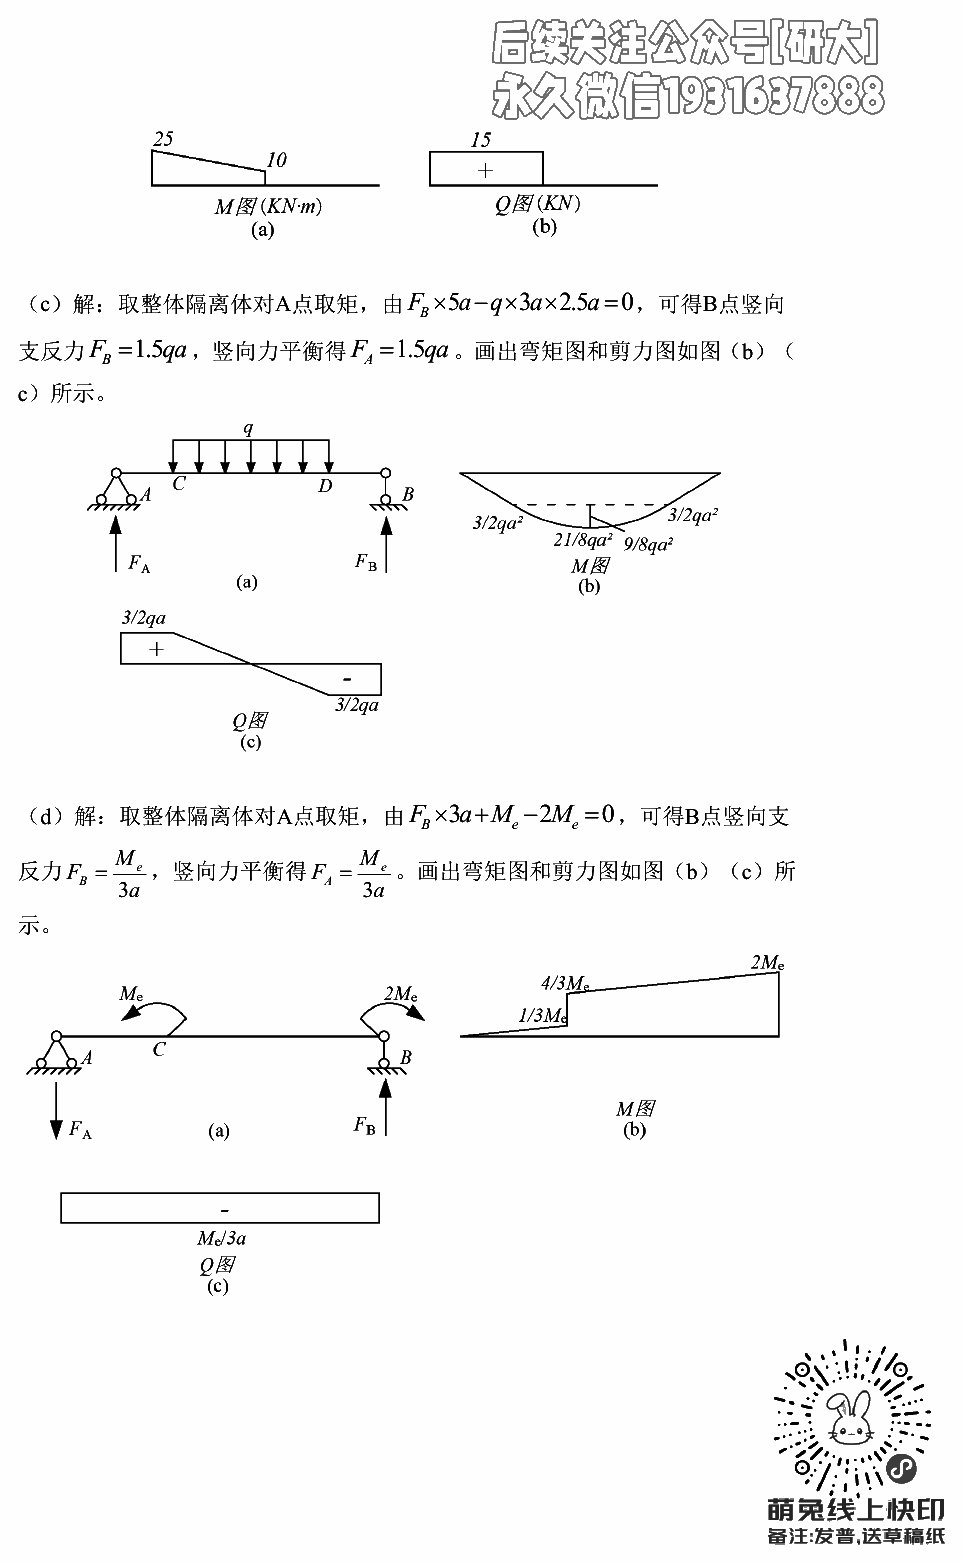
\includegraphics[width=0.96\textwidth,height=0.82\textheight,keepaspectratio]{images/c03_answer_1_p04.png}
\par\small 作业与答案（去水印版），第 4/19 页
\end{center}
\clearpage
\begin{center}
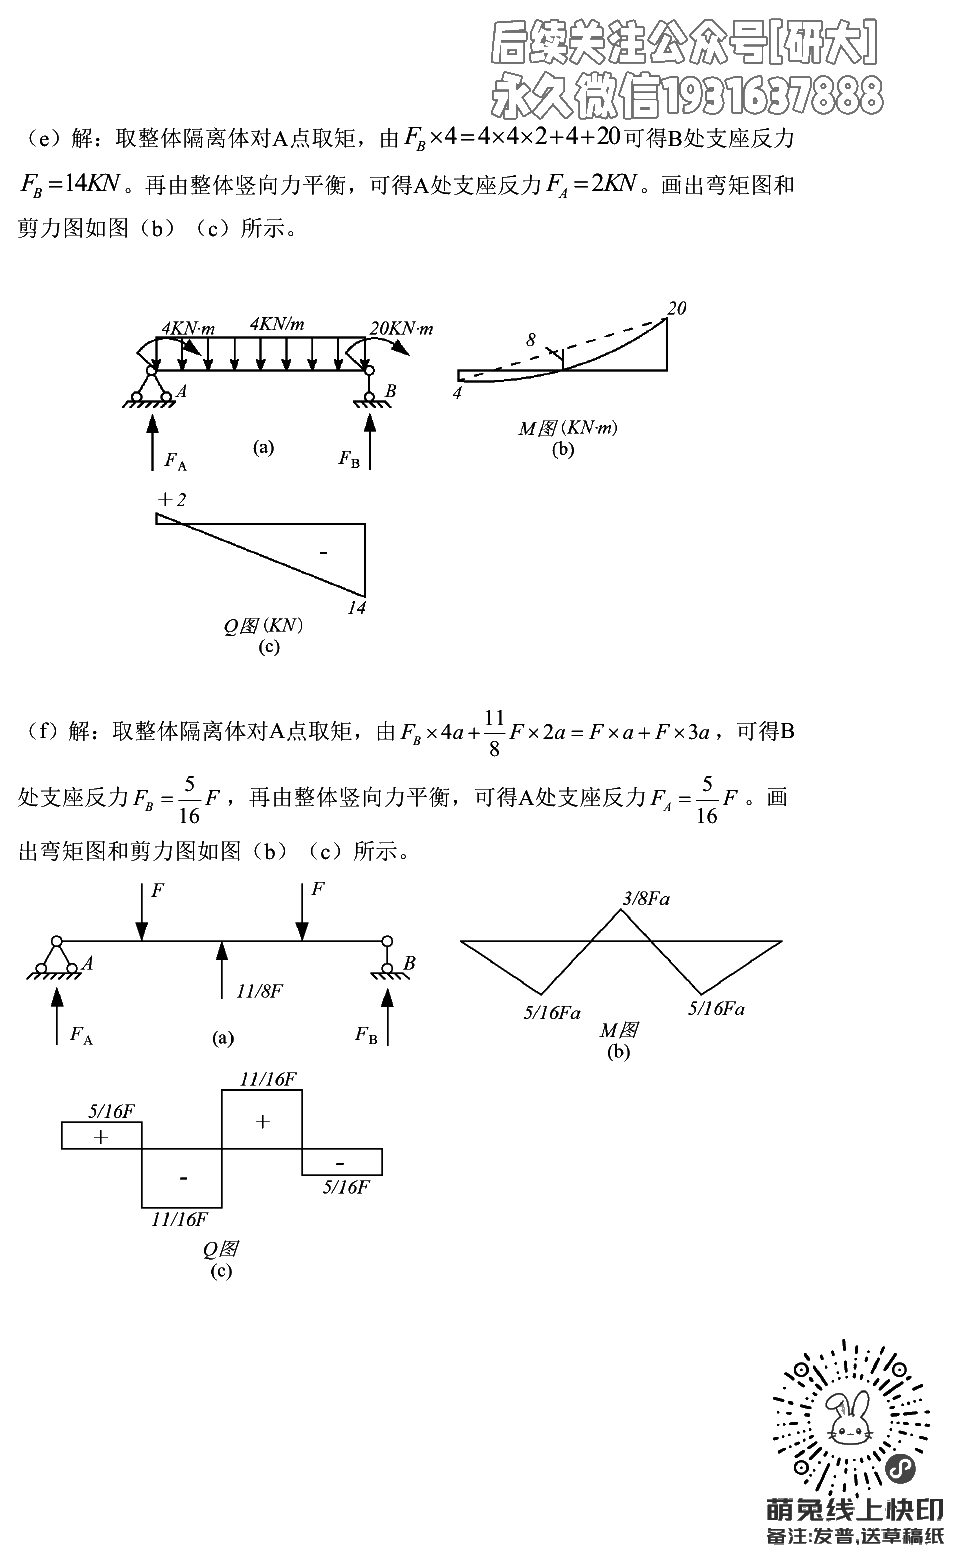
\includegraphics[width=0.96\textwidth,height=0.82\textheight,keepaspectratio]{images/c03_answer_1_p05.png}
\par\small 作业与答案（去水印版），第 5/19 页
\end{center}
\clearpage
\begin{center}
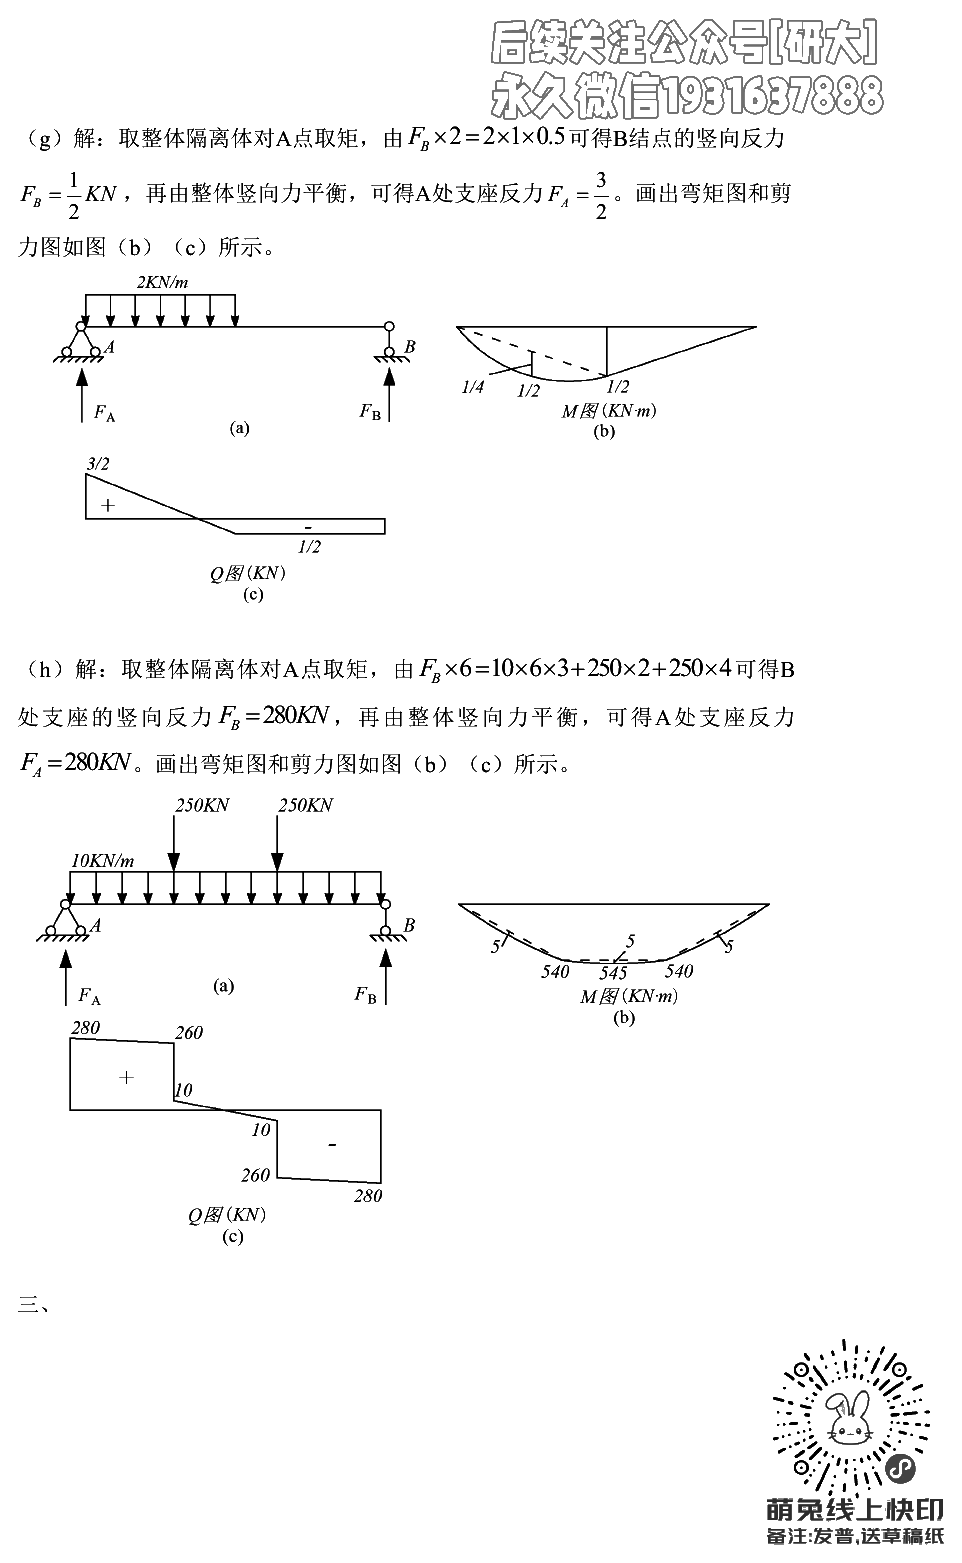
\includegraphics[width=0.96\textwidth,height=0.82\textheight,keepaspectratio]{images/c03_answer_1_p06.png}
\par\small 作业与答案（去水印版），第 6/19 页
\end{center}
\clearpage
\begin{center}
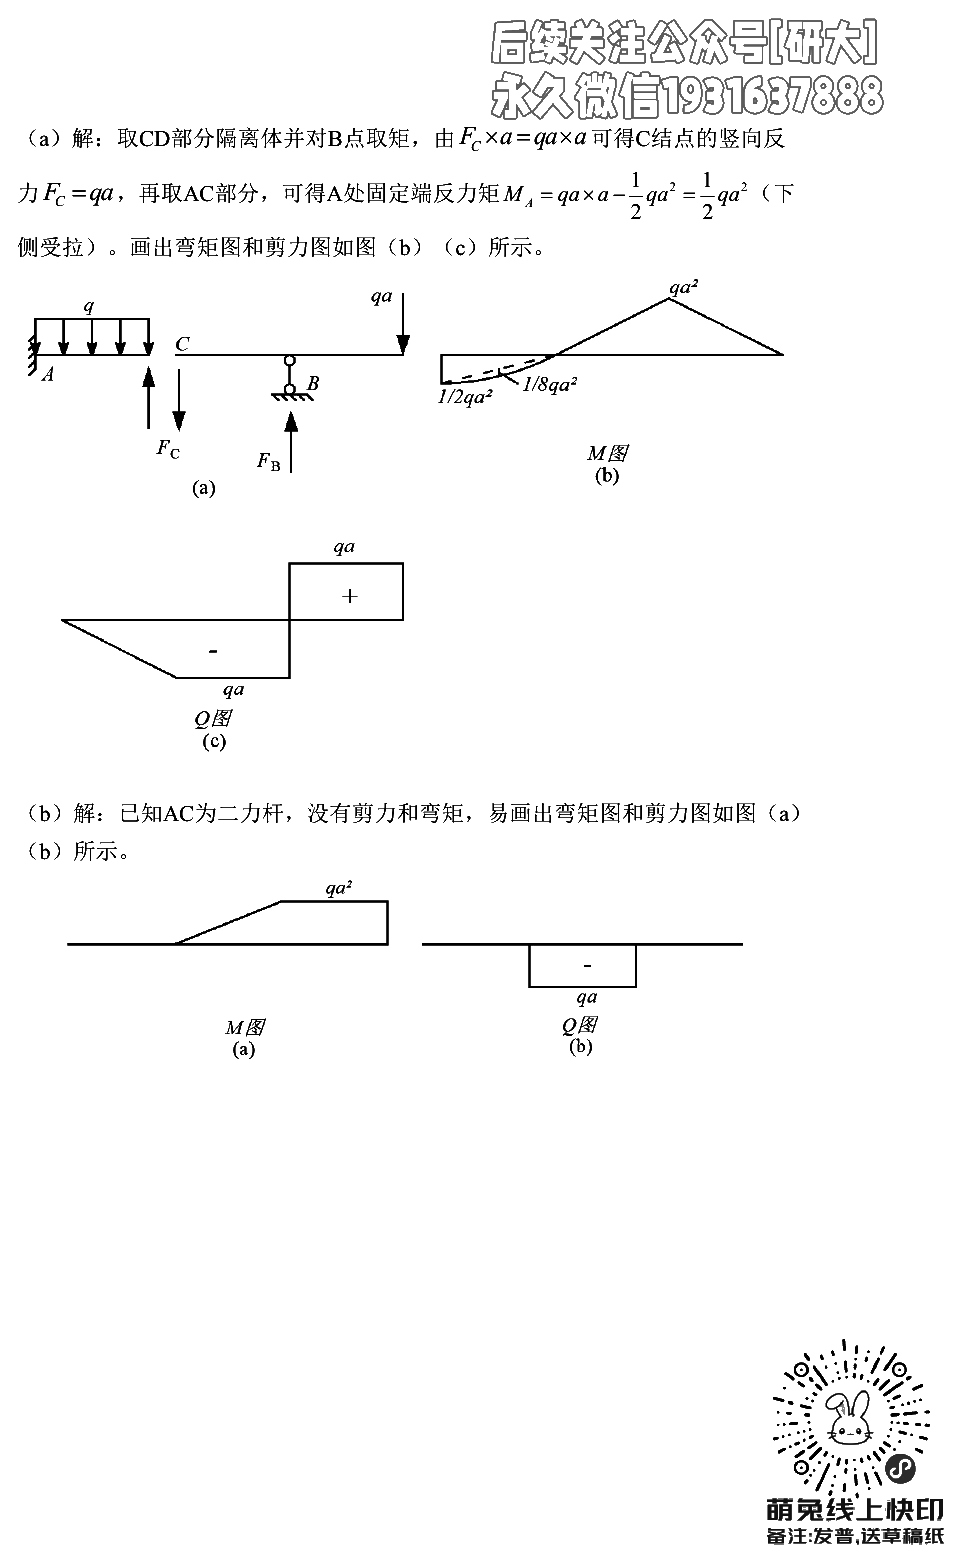
\includegraphics[width=0.96\textwidth,height=0.82\textheight,keepaspectratio]{images/c03_answer_1_p07.png}
\par\small 作业与答案（去水印版），第 7/19 页
\end{center}
\clearpage
\begin{center}
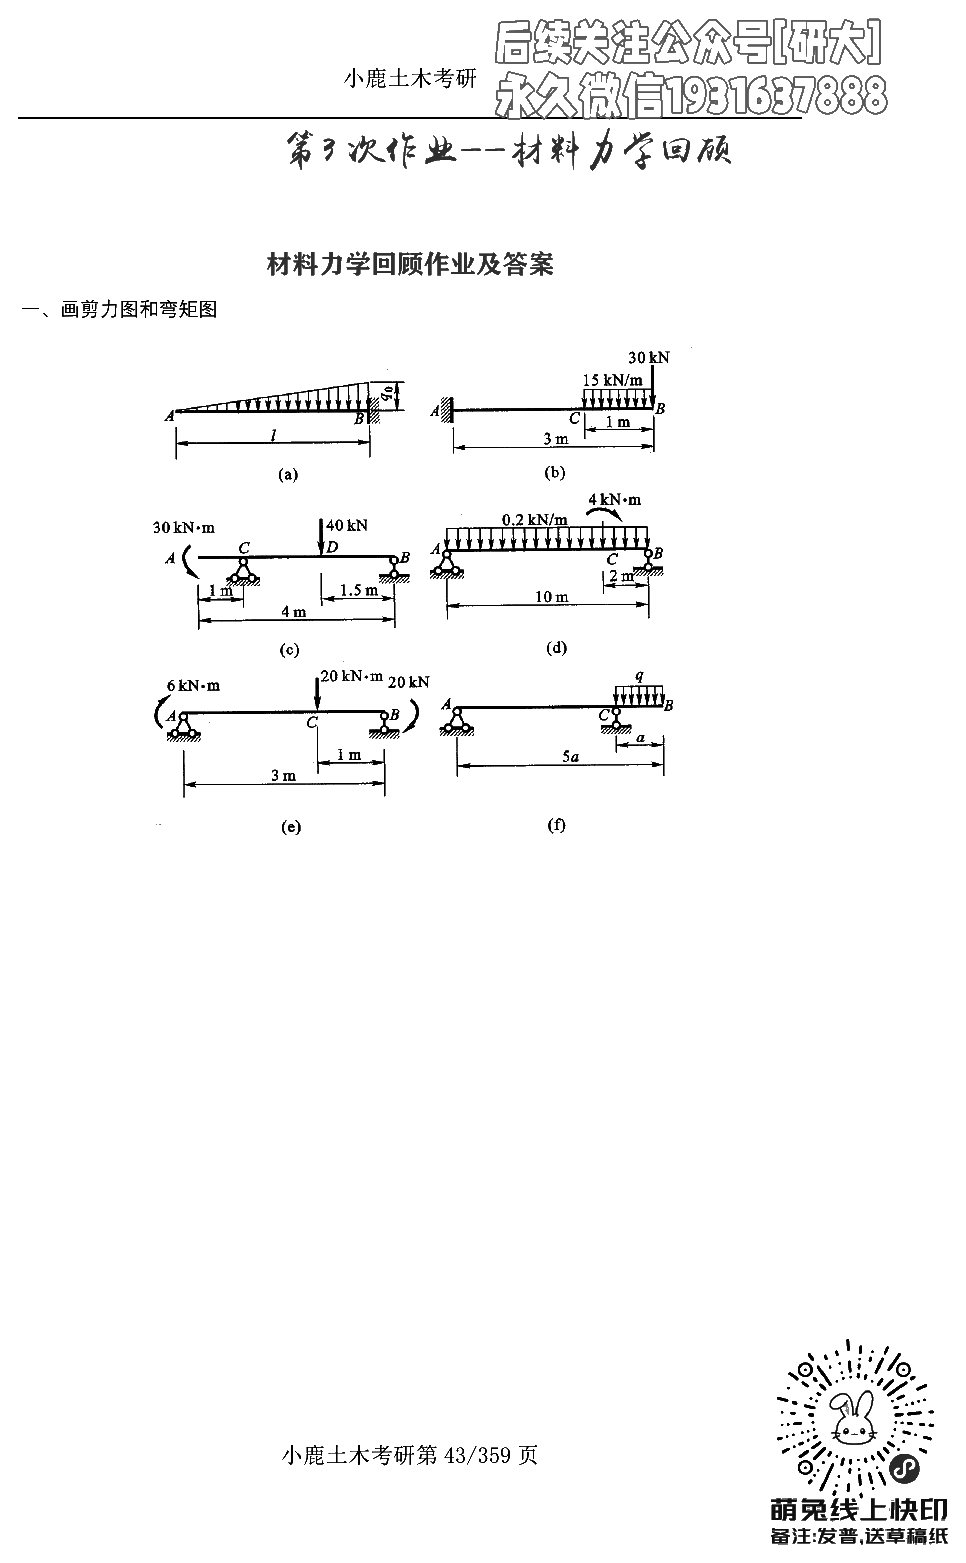
\includegraphics[width=0.96\textwidth,height=0.82\textheight,keepaspectratio]{images/c03_answer_2_p01.png}
\par\small 作业与答案（去水印版），第 8/19 页
\end{center}
\clearpage
\begin{center}
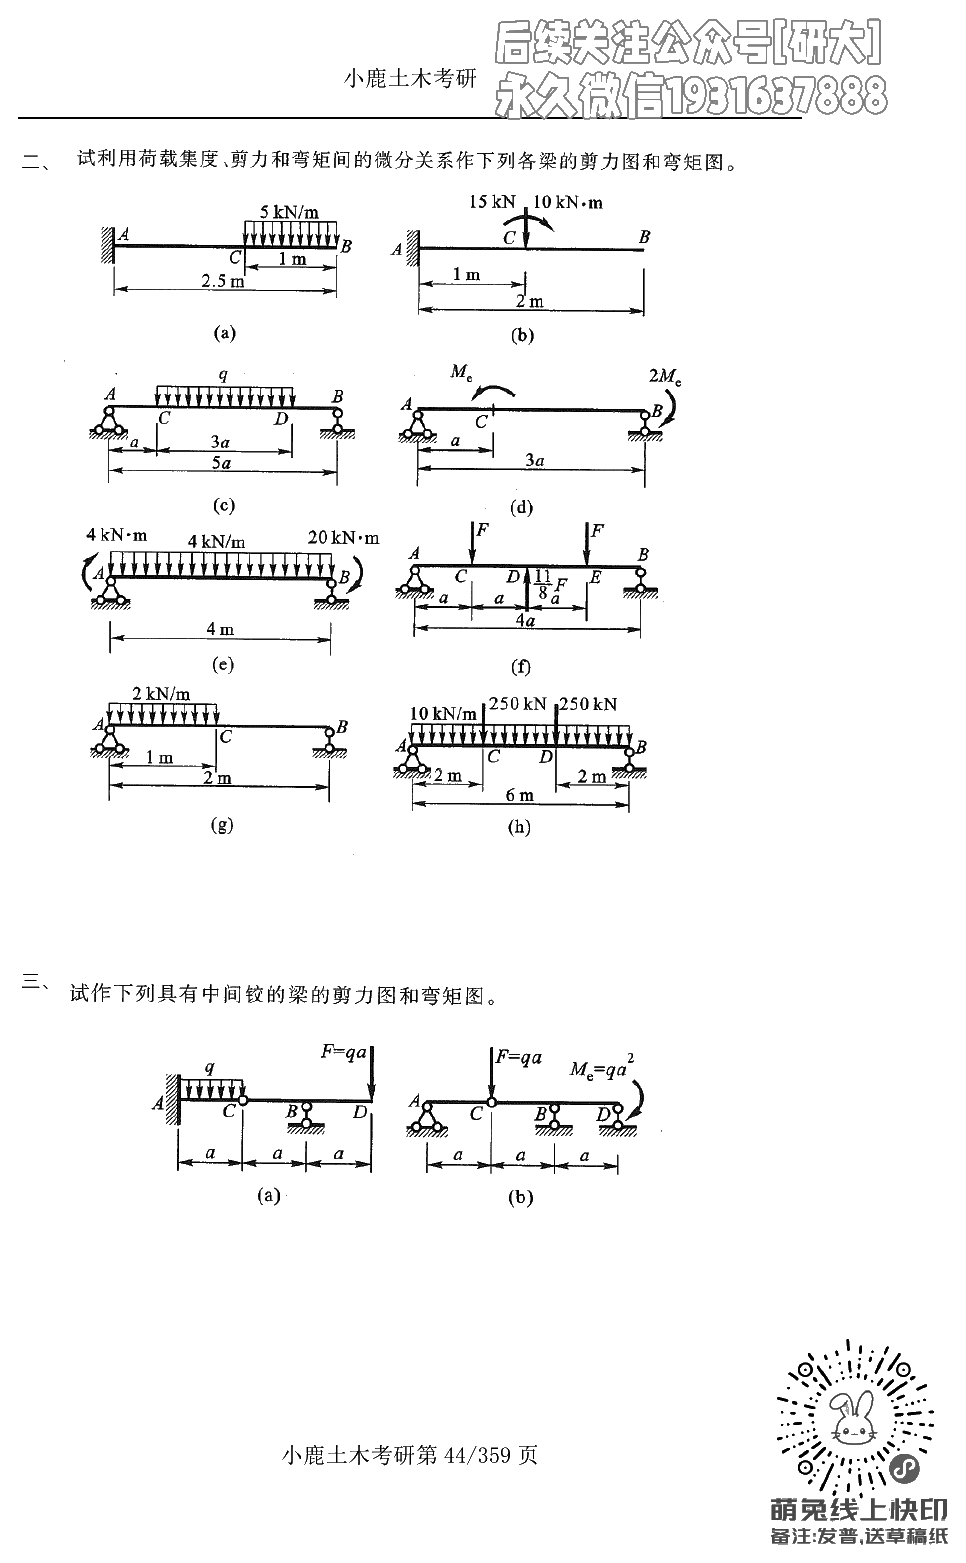
\includegraphics[width=0.96\textwidth,height=0.82\textheight,keepaspectratio]{images/c03_answer_2_p02.png}
\par\small 作业与答案（去水印版），第 9/19 页
\end{center}
\clearpage
\begin{center}
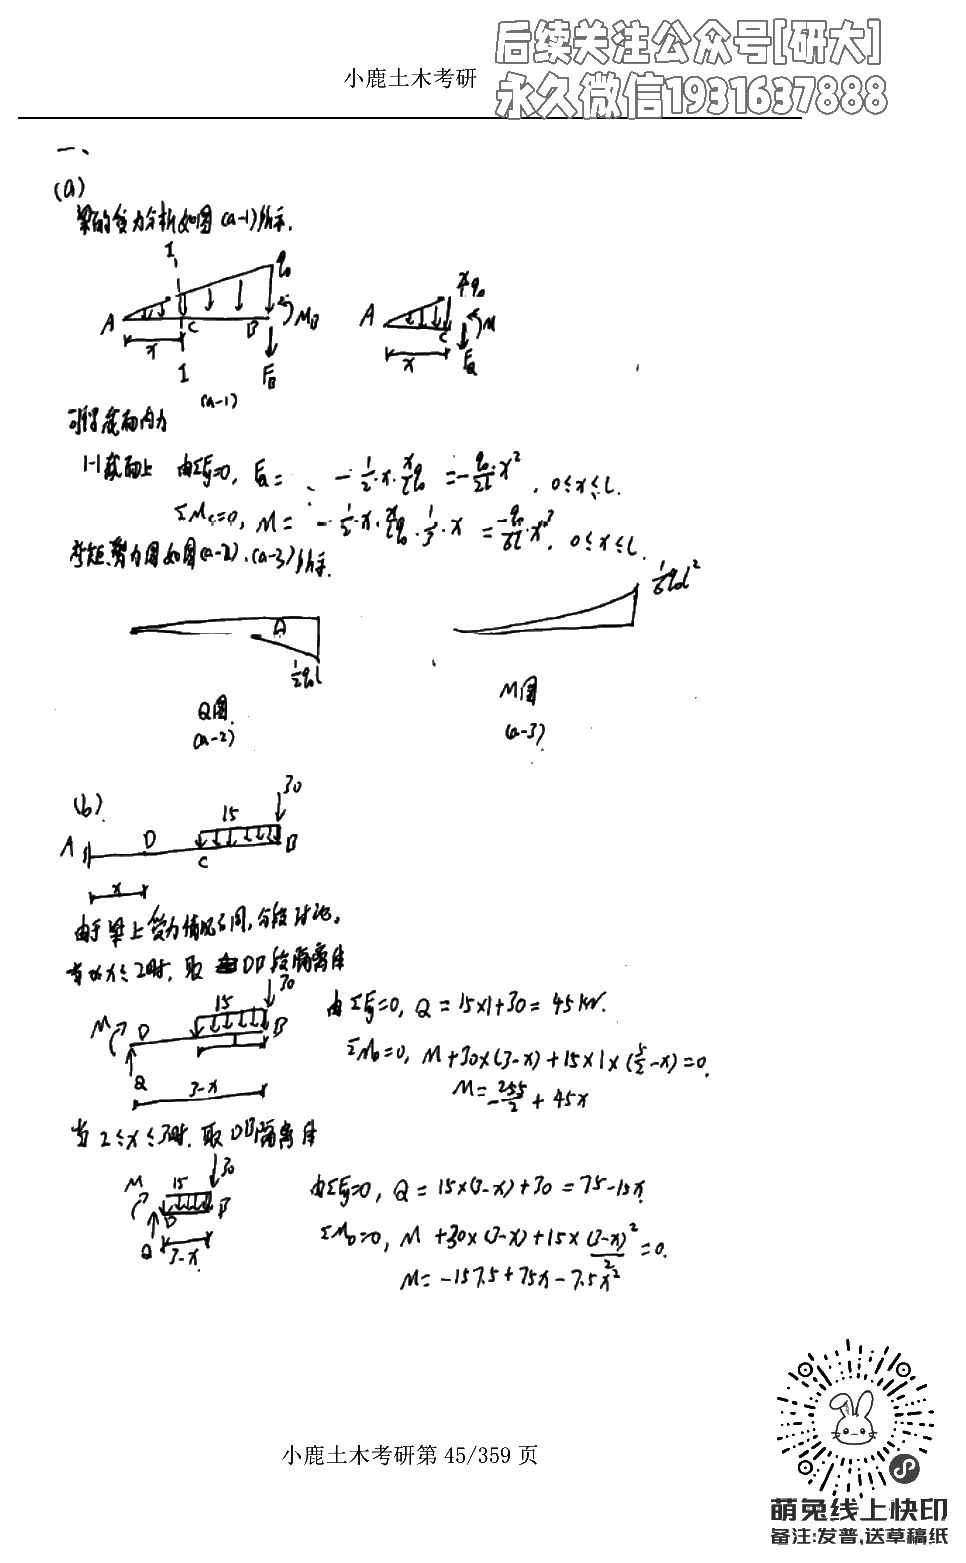
\includegraphics[width=0.96\textwidth,height=0.82\textheight,keepaspectratio]{images/c03_answer_2_p03.png}
\par\small 作业与答案（去水印版），第 10/19 页
\end{center}
\clearpage
\begin{center}
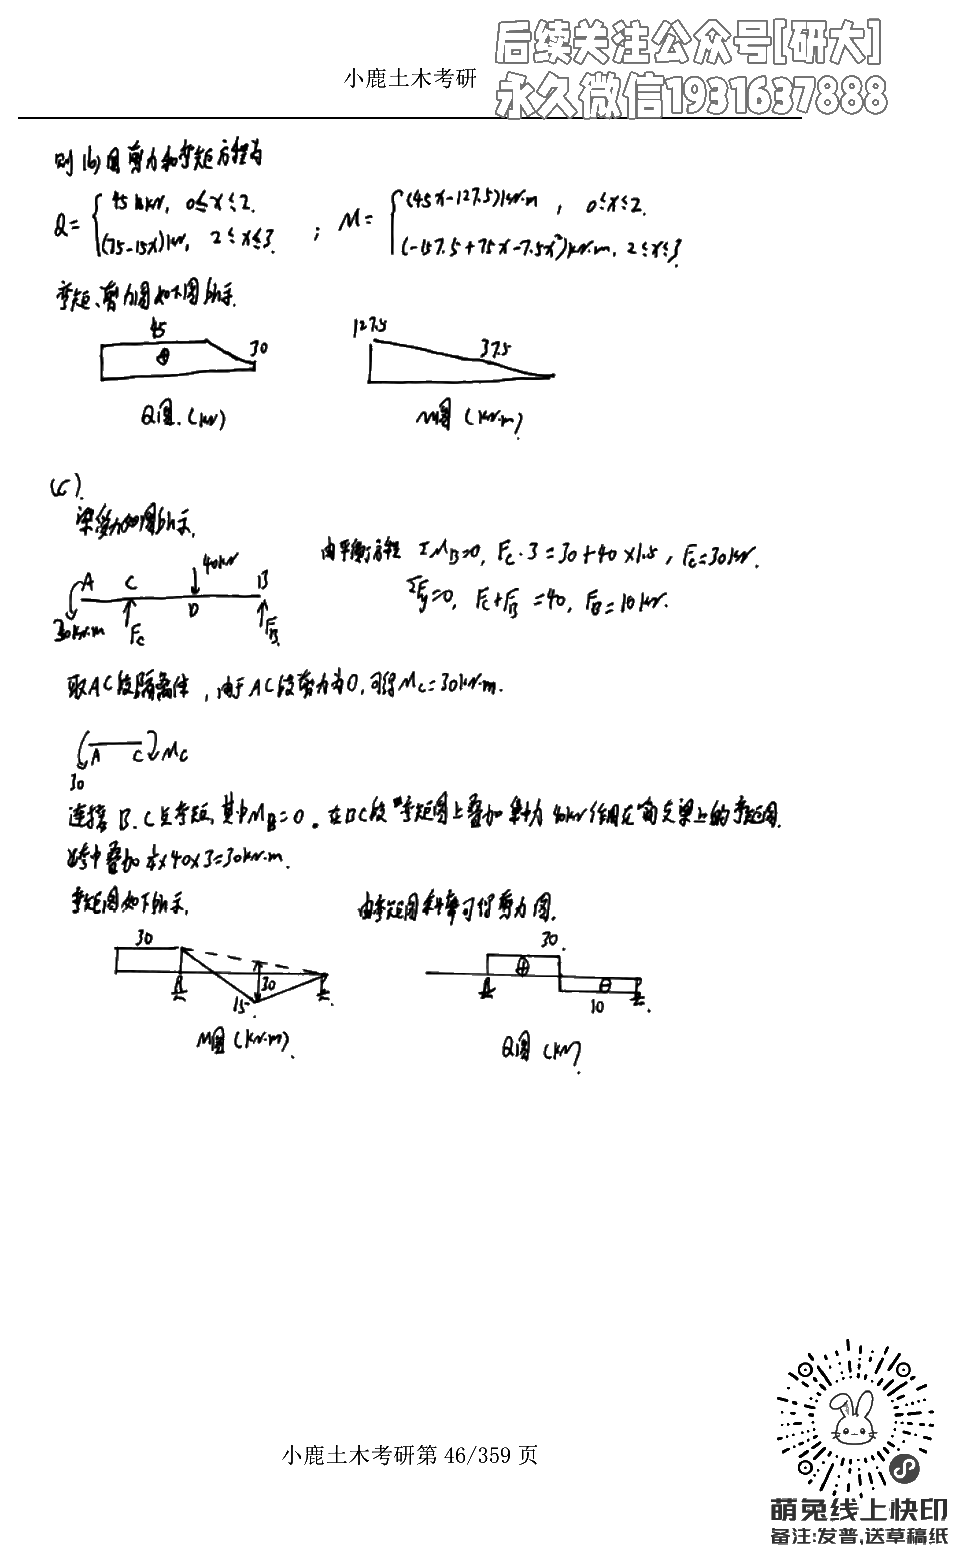
\includegraphics[width=0.96\textwidth,height=0.82\textheight,keepaspectratio]{images/c03_answer_2_p04.png}
\par\small 作业与答案（去水印版），第 11/19 页
\end{center}
\clearpage
\begin{center}
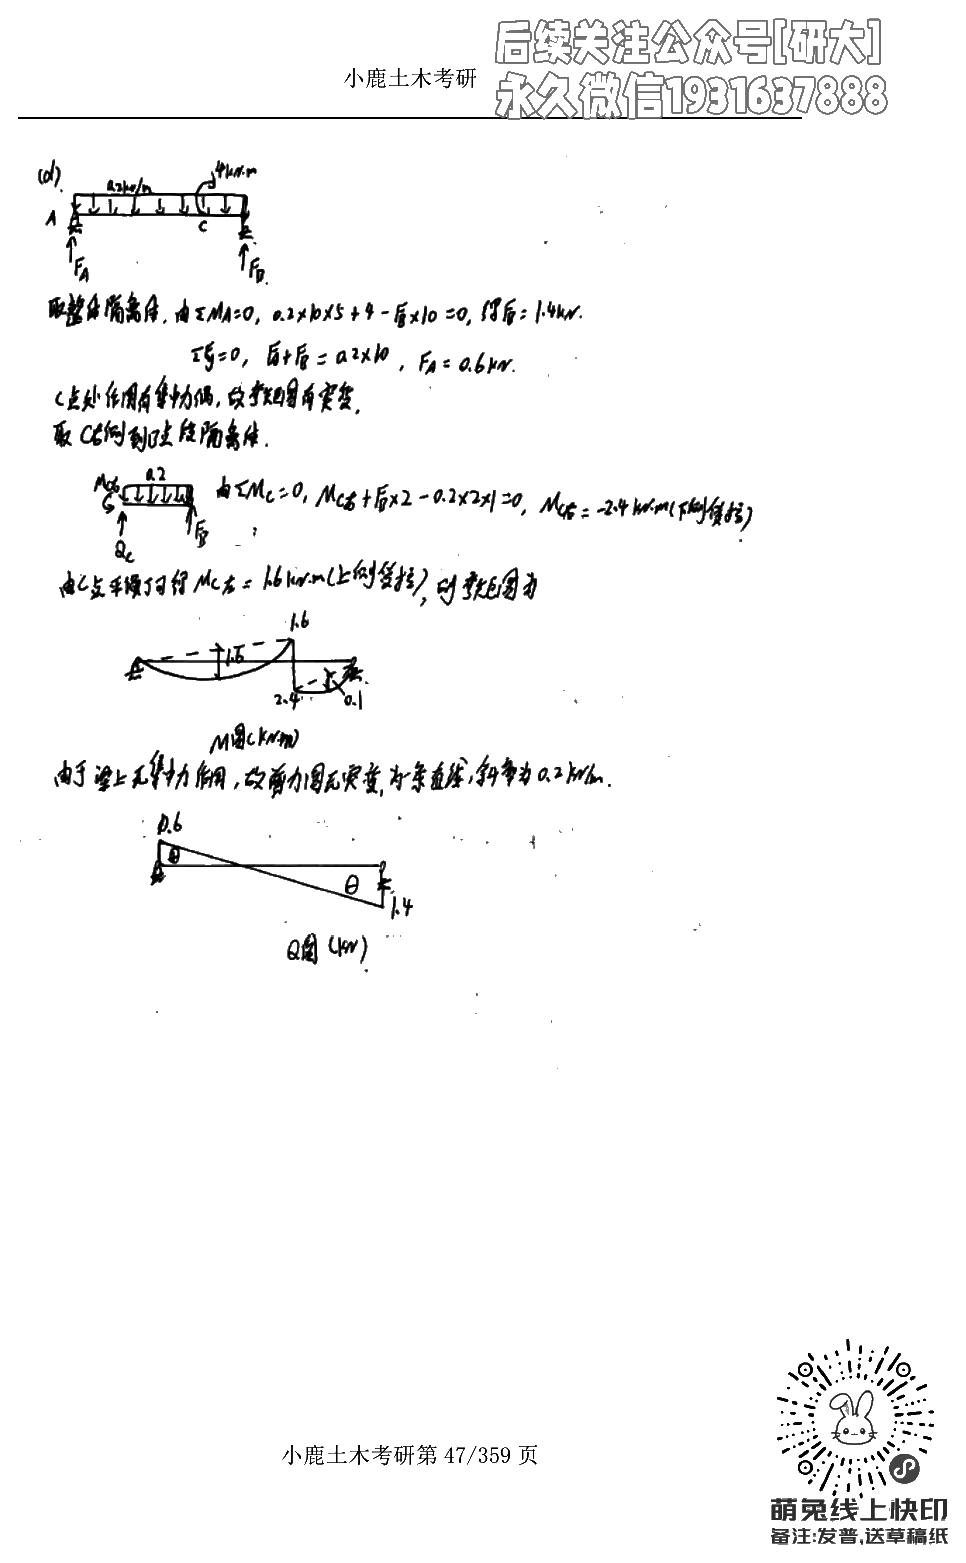
\includegraphics[width=0.96\textwidth,height=0.82\textheight,keepaspectratio]{images/c03_answer_2_p05.png}
\par\small 作业与答案（去水印版），第 12/19 页
\end{center}
\clearpage
\begin{center}
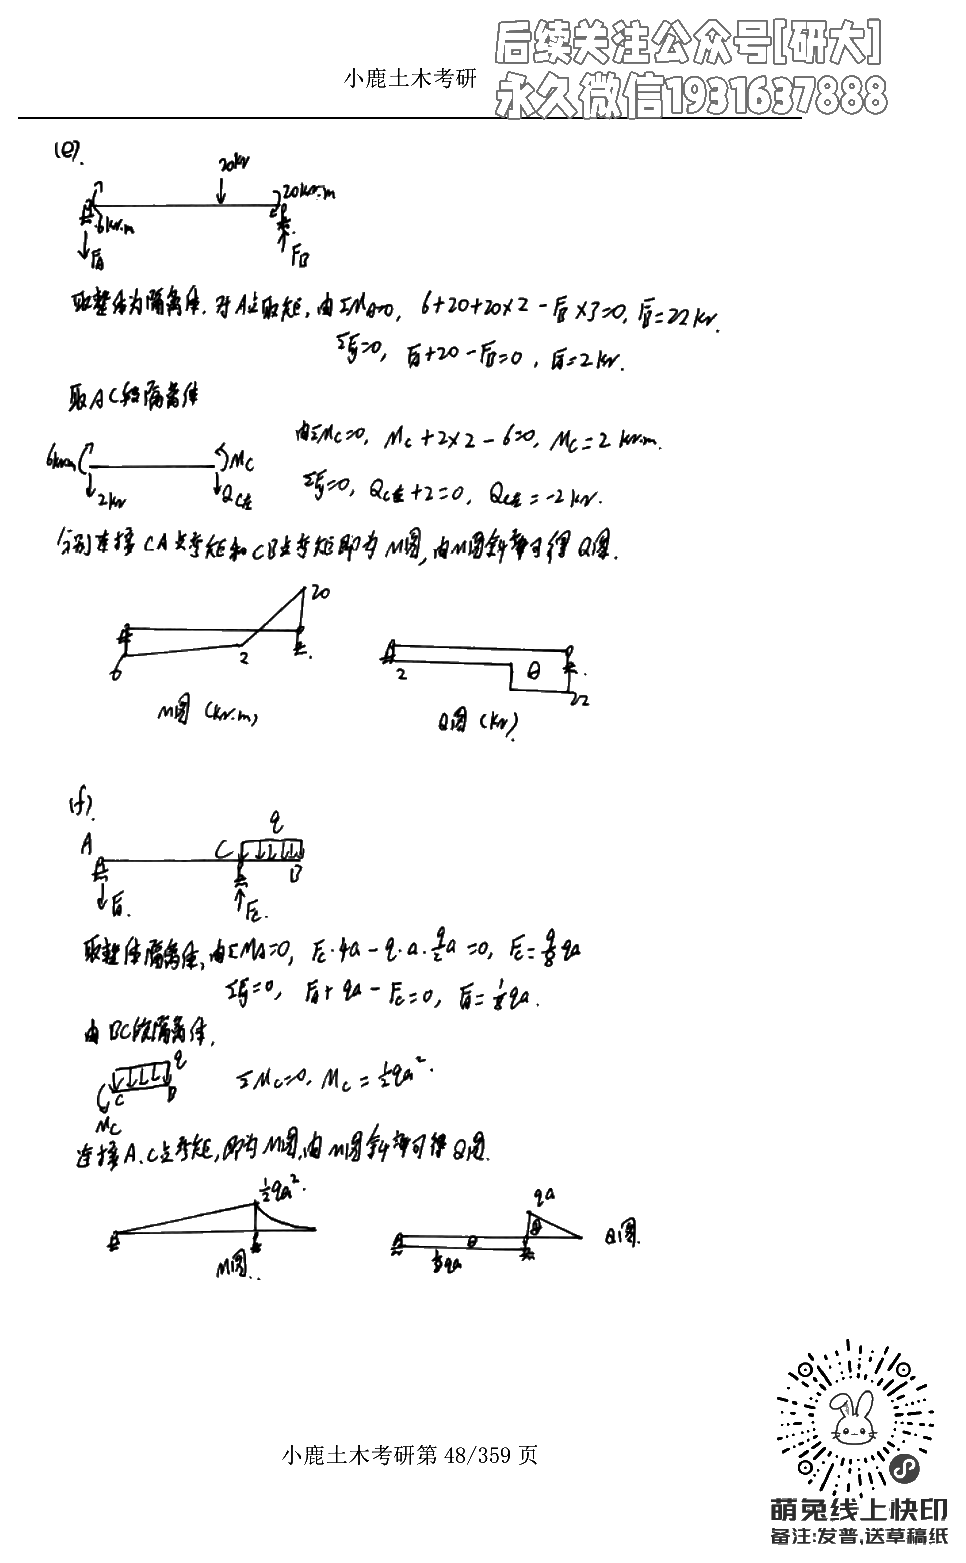
\includegraphics[width=0.96\textwidth,height=0.82\textheight,keepaspectratio]{images/c03_answer_2_p06.png}
\par\small 作业与答案（去水印版），第 13/19 页
\end{center}
\clearpage
\begin{center}
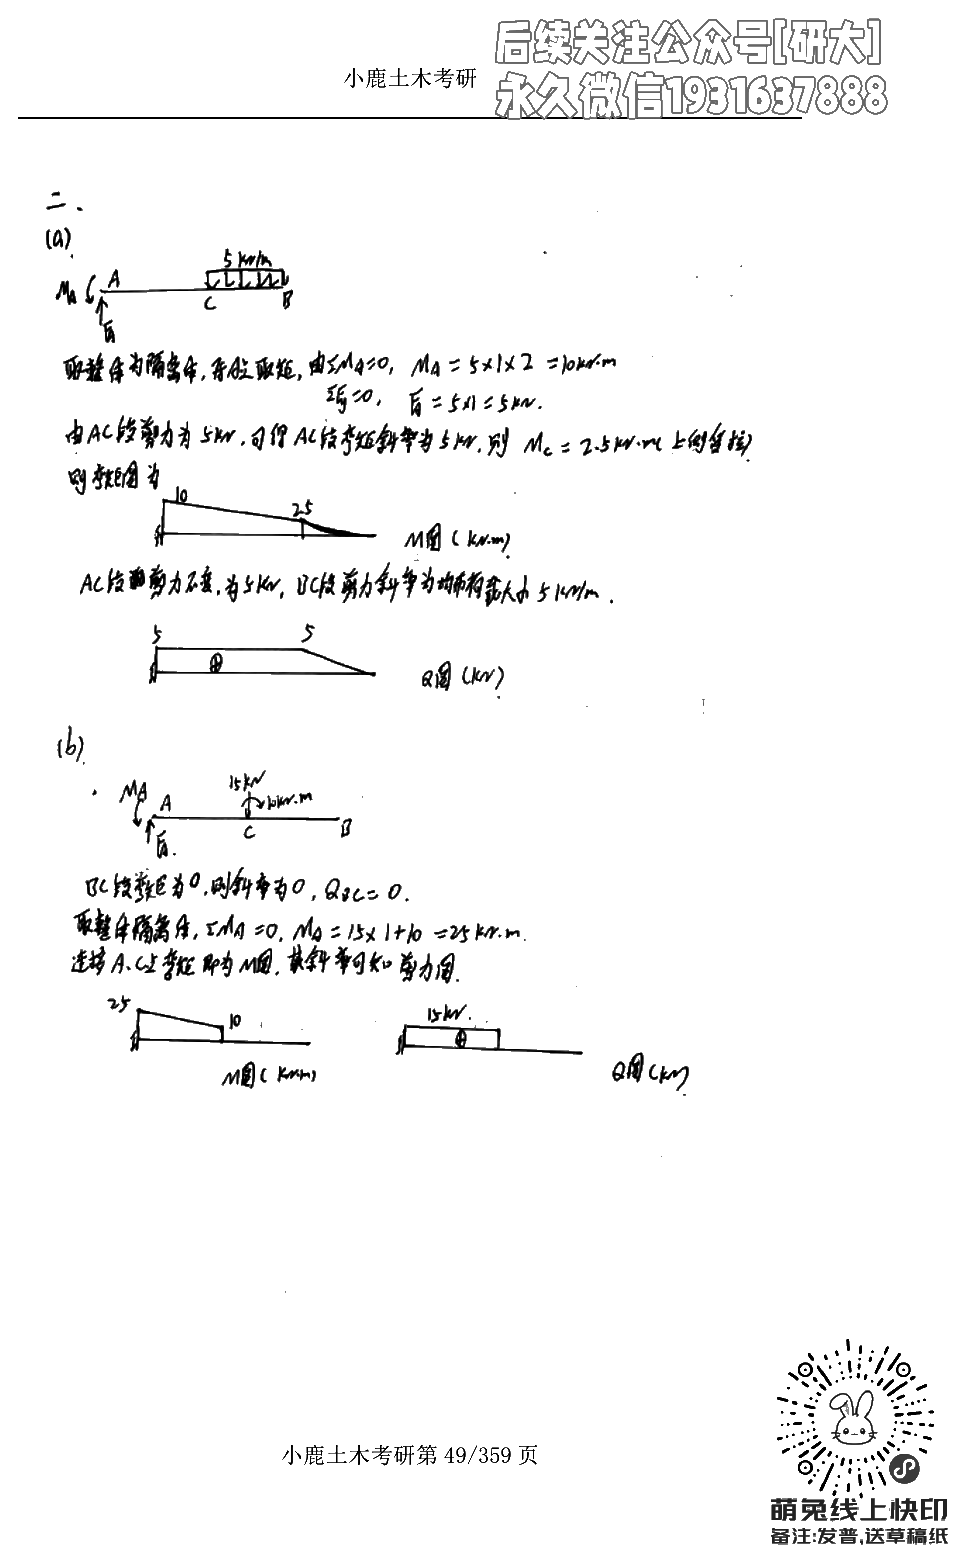
\includegraphics[width=0.96\textwidth,height=0.82\textheight,keepaspectratio]{images/c03_answer_2_p07.png}
\par\small 作业与答案（去水印版），第 14/19 页
\end{center}
\clearpage
\begin{center}
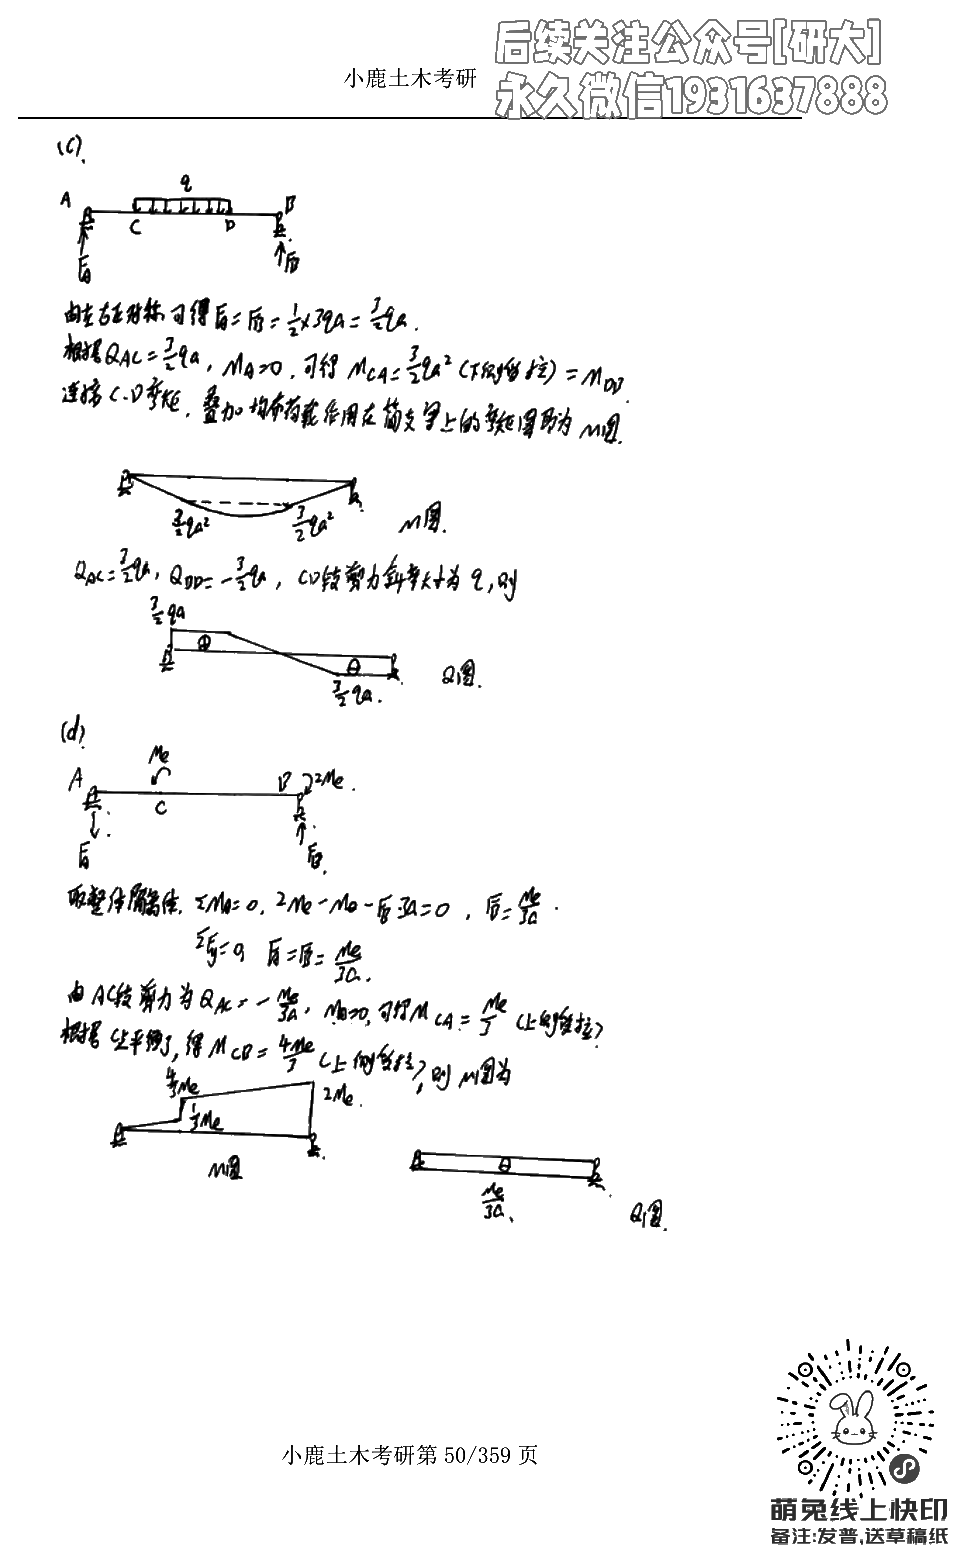
\includegraphics[width=0.96\textwidth,height=0.82\textheight,keepaspectratio]{images/c03_answer_2_p08.png}
\par\small 作业与答案（去水印版），第 15/19 页
\end{center}
\clearpage
\begin{center}
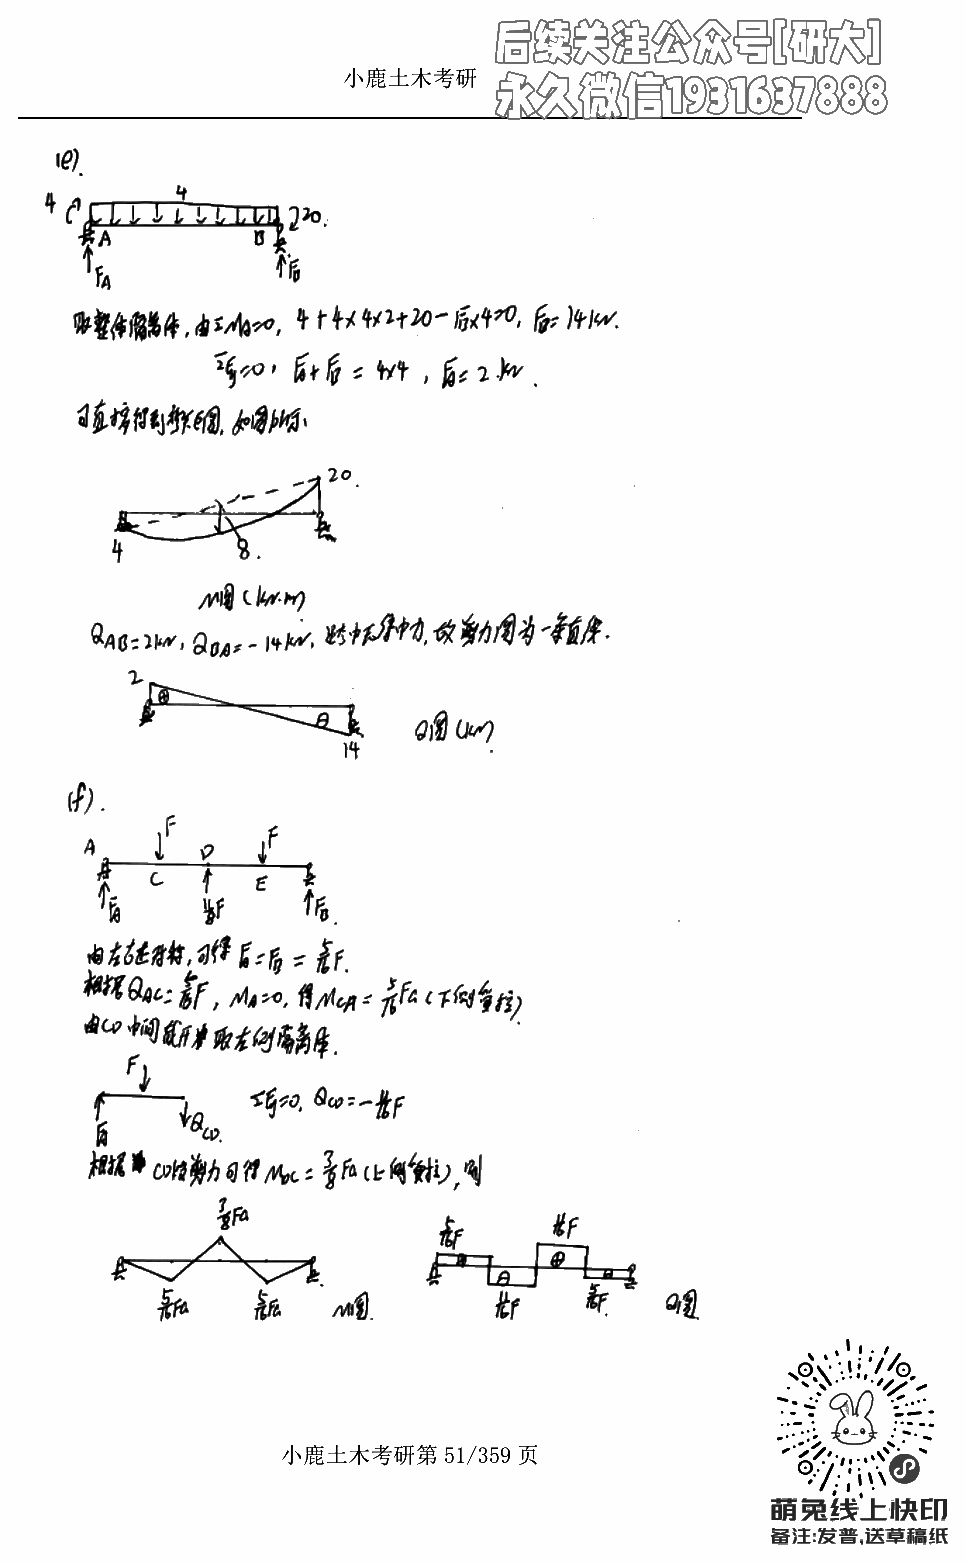
\includegraphics[width=0.96\textwidth,height=0.82\textheight,keepaspectratio]{images/c03_answer_2_p09.png}
\par\small 作业与答案（去水印版），第 16/19 页
\end{center}
\clearpage
\begin{center}
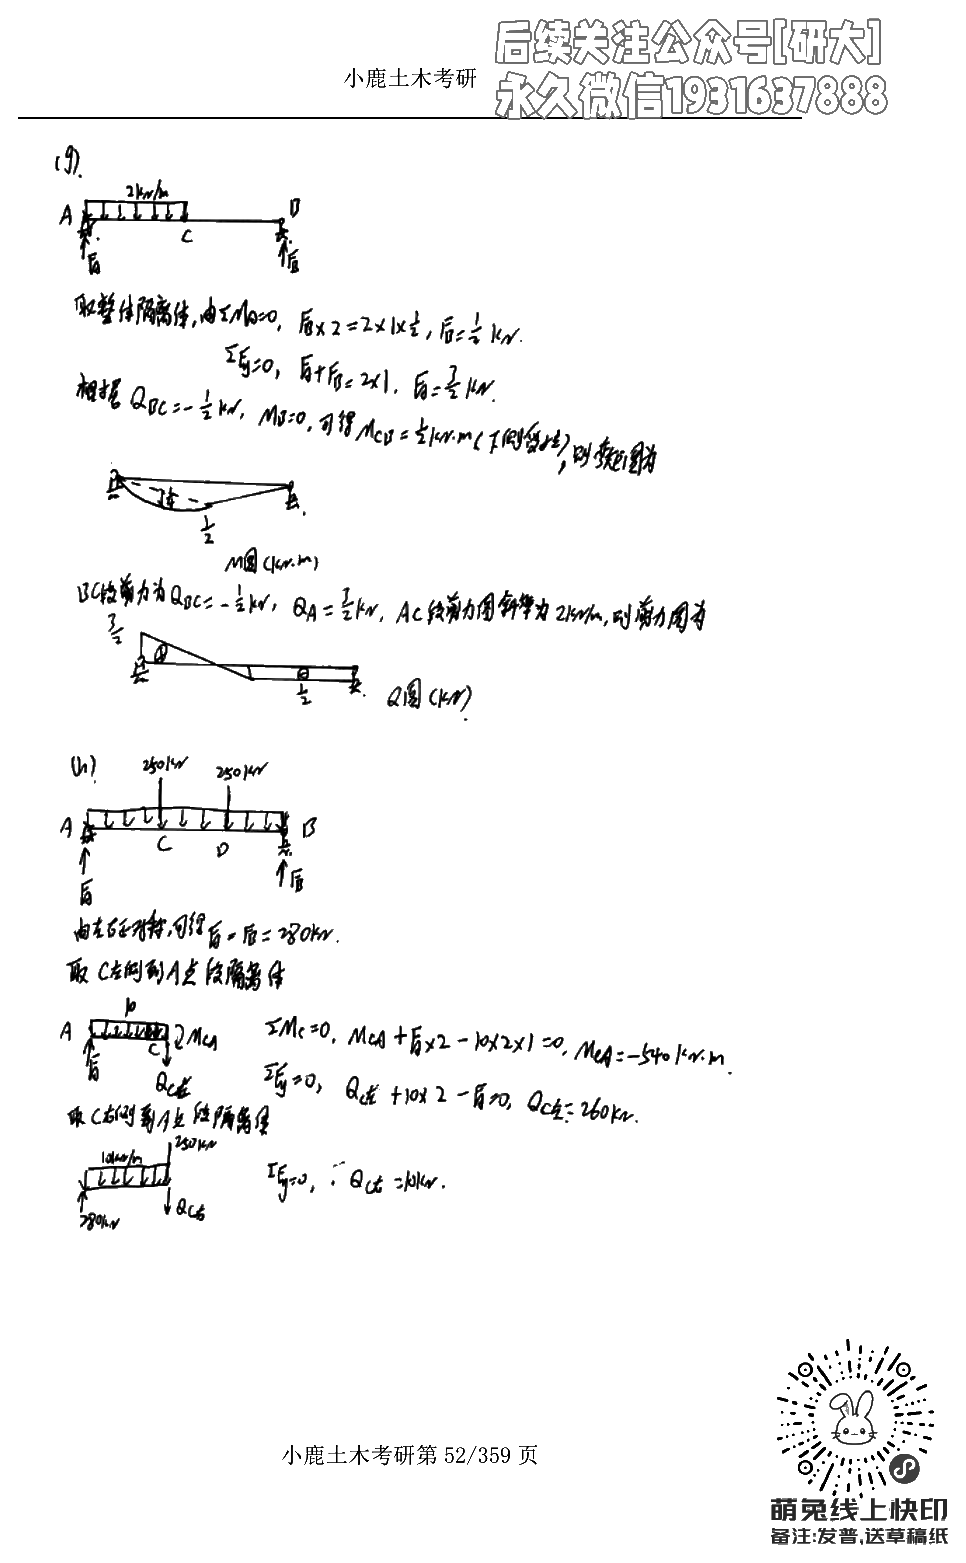
\includegraphics[width=0.96\textwidth,height=0.82\textheight,keepaspectratio]{images/c03_answer_2_p10.png}
\par\small 作业与答案（去水印版），第 17/19 页
\end{center}
\clearpage
\begin{center}
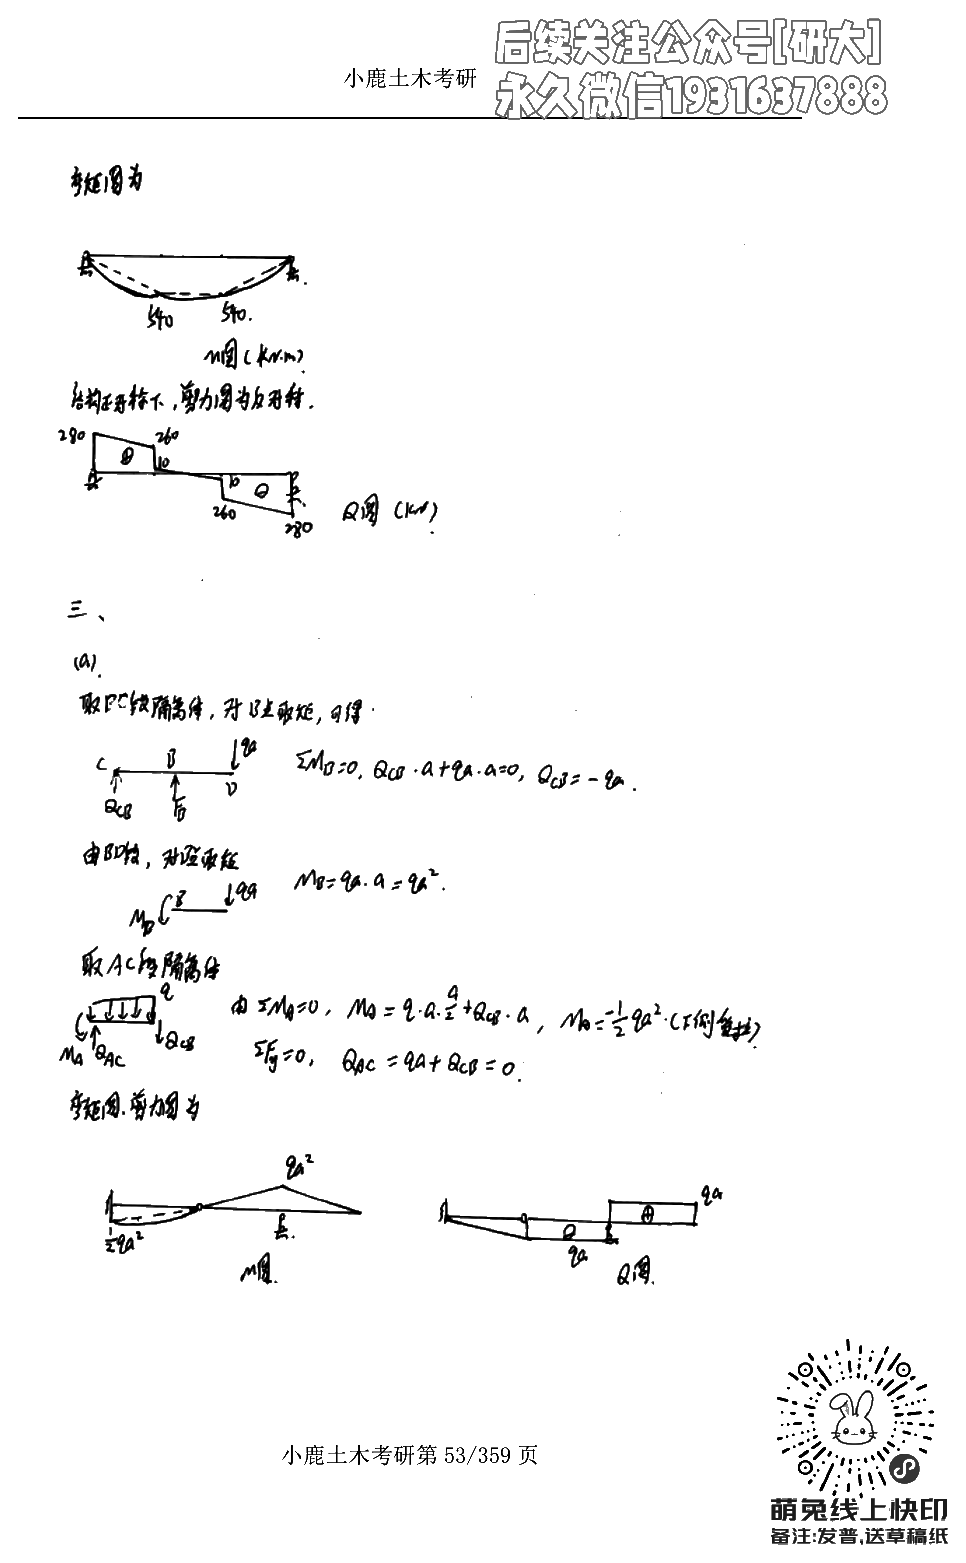
\includegraphics[width=0.96\textwidth,height=0.82\textheight,keepaspectratio]{images/c03_answer_2_p11.png}
\par\small 作业与答案（去水印版），第 18/19 页
\end{center}
\clearpage
\begin{center}
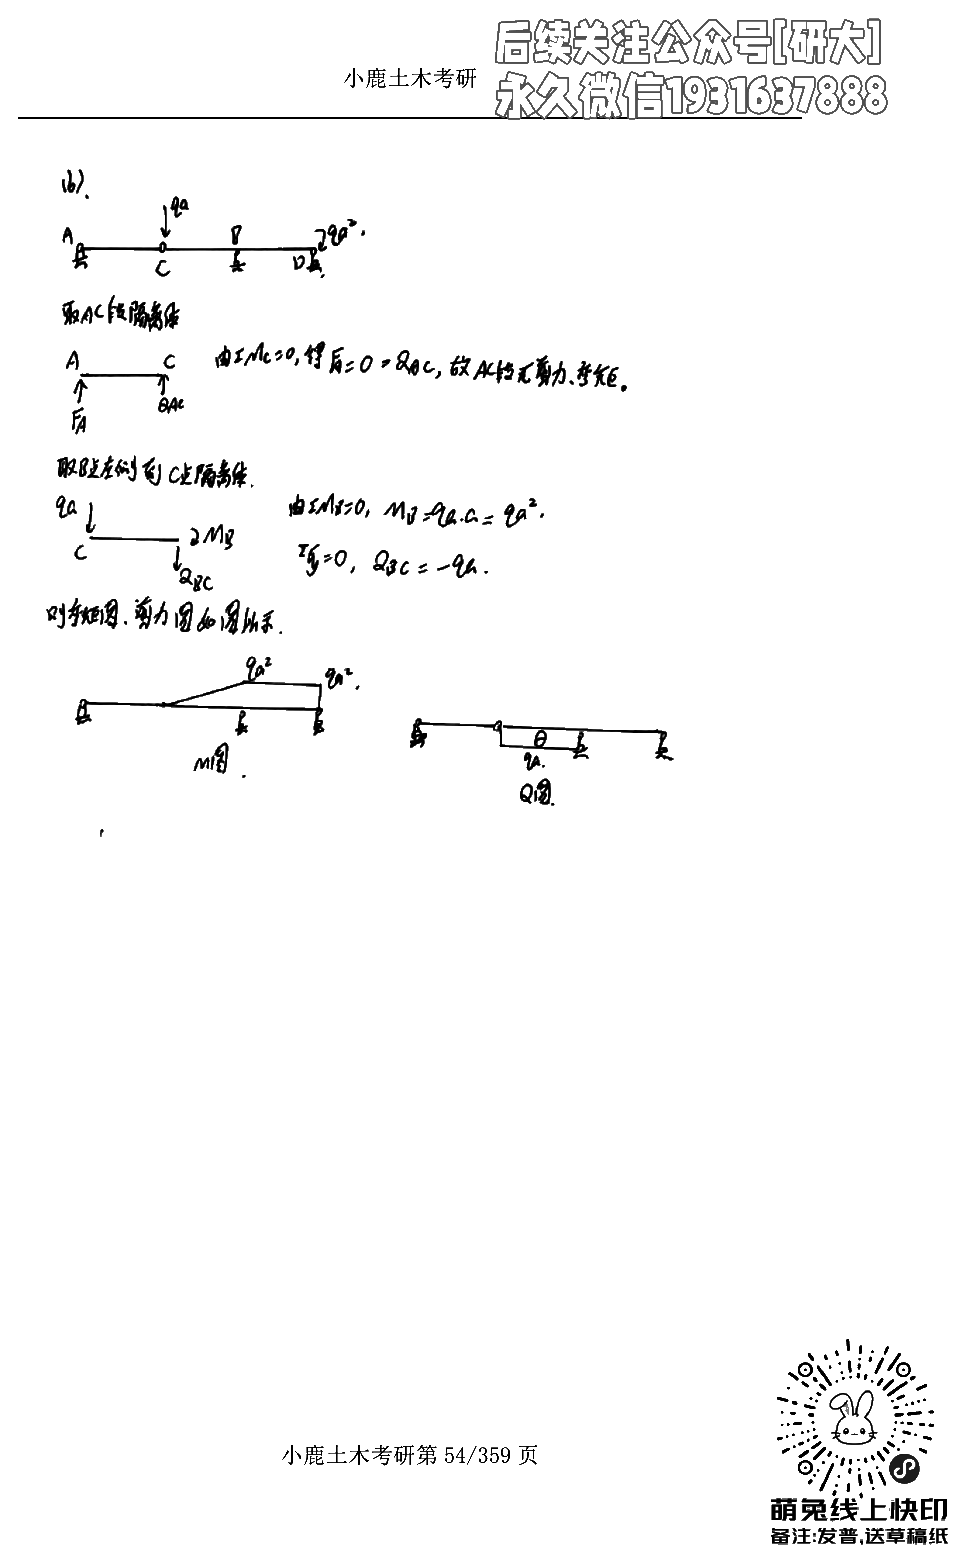
\includegraphics[width=0.96\textwidth,height=0.82\textheight,keepaspectratio]{images/c03_answer_2_p12.png}
\par\small 作业与答案（去水印版），第 19/19 页
\end{center}
\clearpage
\section{讲解笔记（去水印版）}
\begin{center}
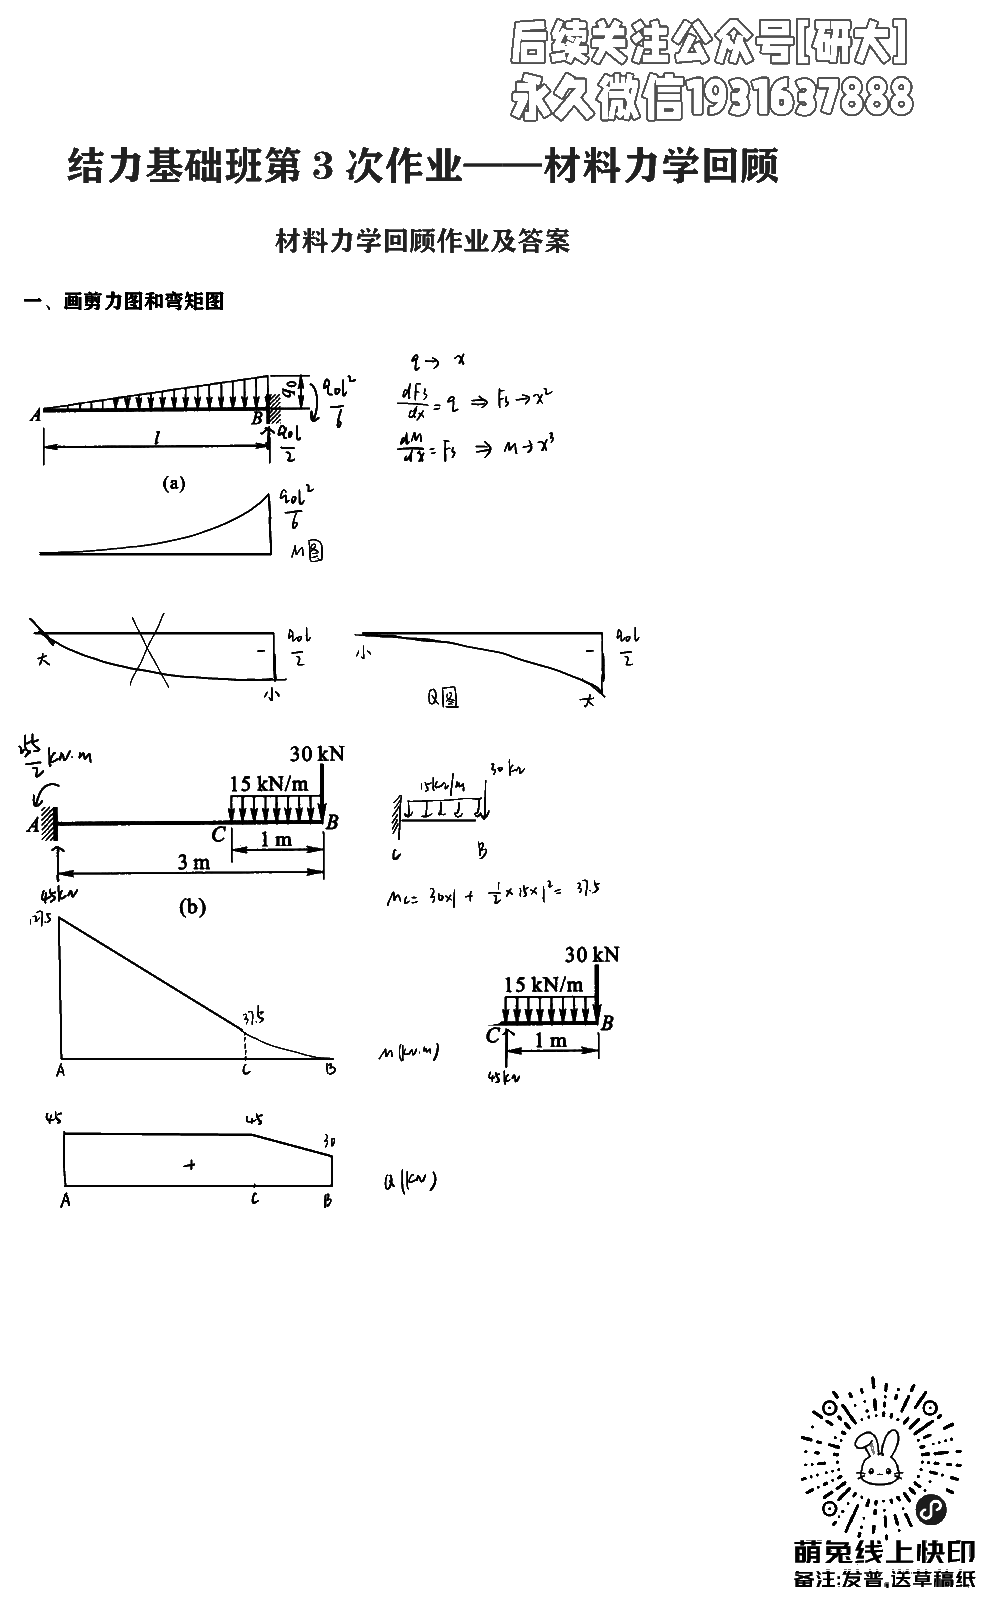
\includegraphics[width=0.96\textwidth,height=0.82\textheight,keepaspectratio]{images/c03_note_p01.png}
\par\small 讲解笔记（去水印版），第 1/9 页
\end{center}
\clearpage
\begin{center}
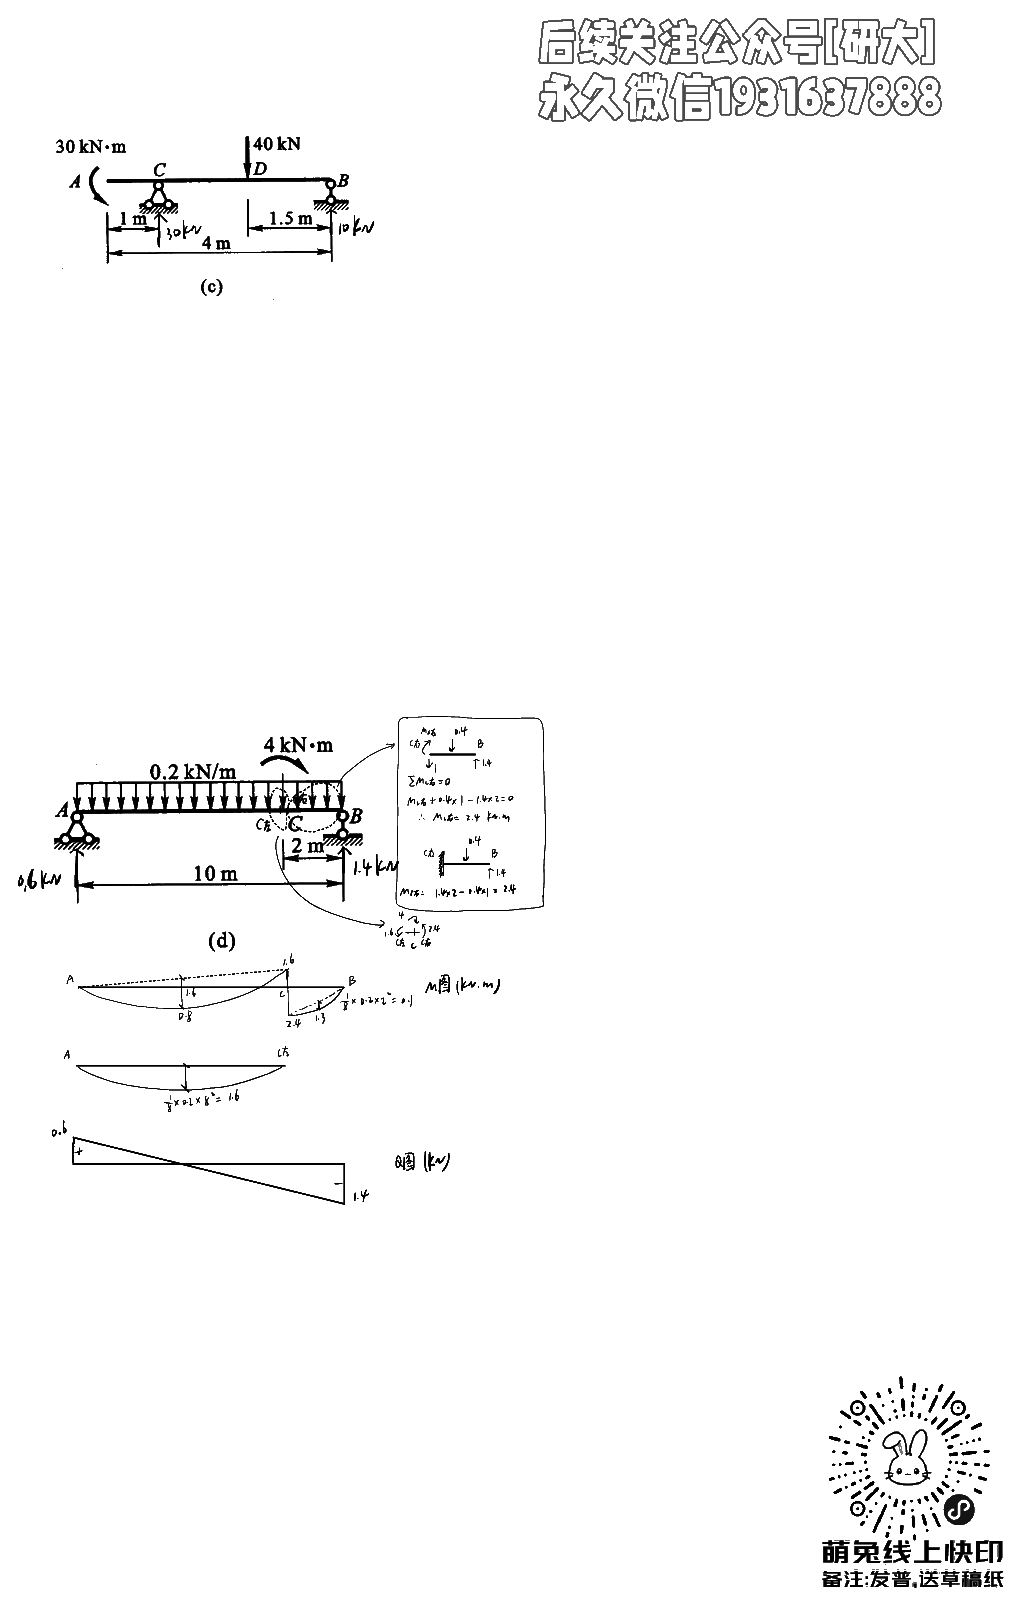
\includegraphics[width=0.96\textwidth,height=0.82\textheight,keepaspectratio]{images/c03_note_p02.png}
\par\small 讲解笔记（去水印版），第 2/9 页
\end{center}
\clearpage
\begin{center}
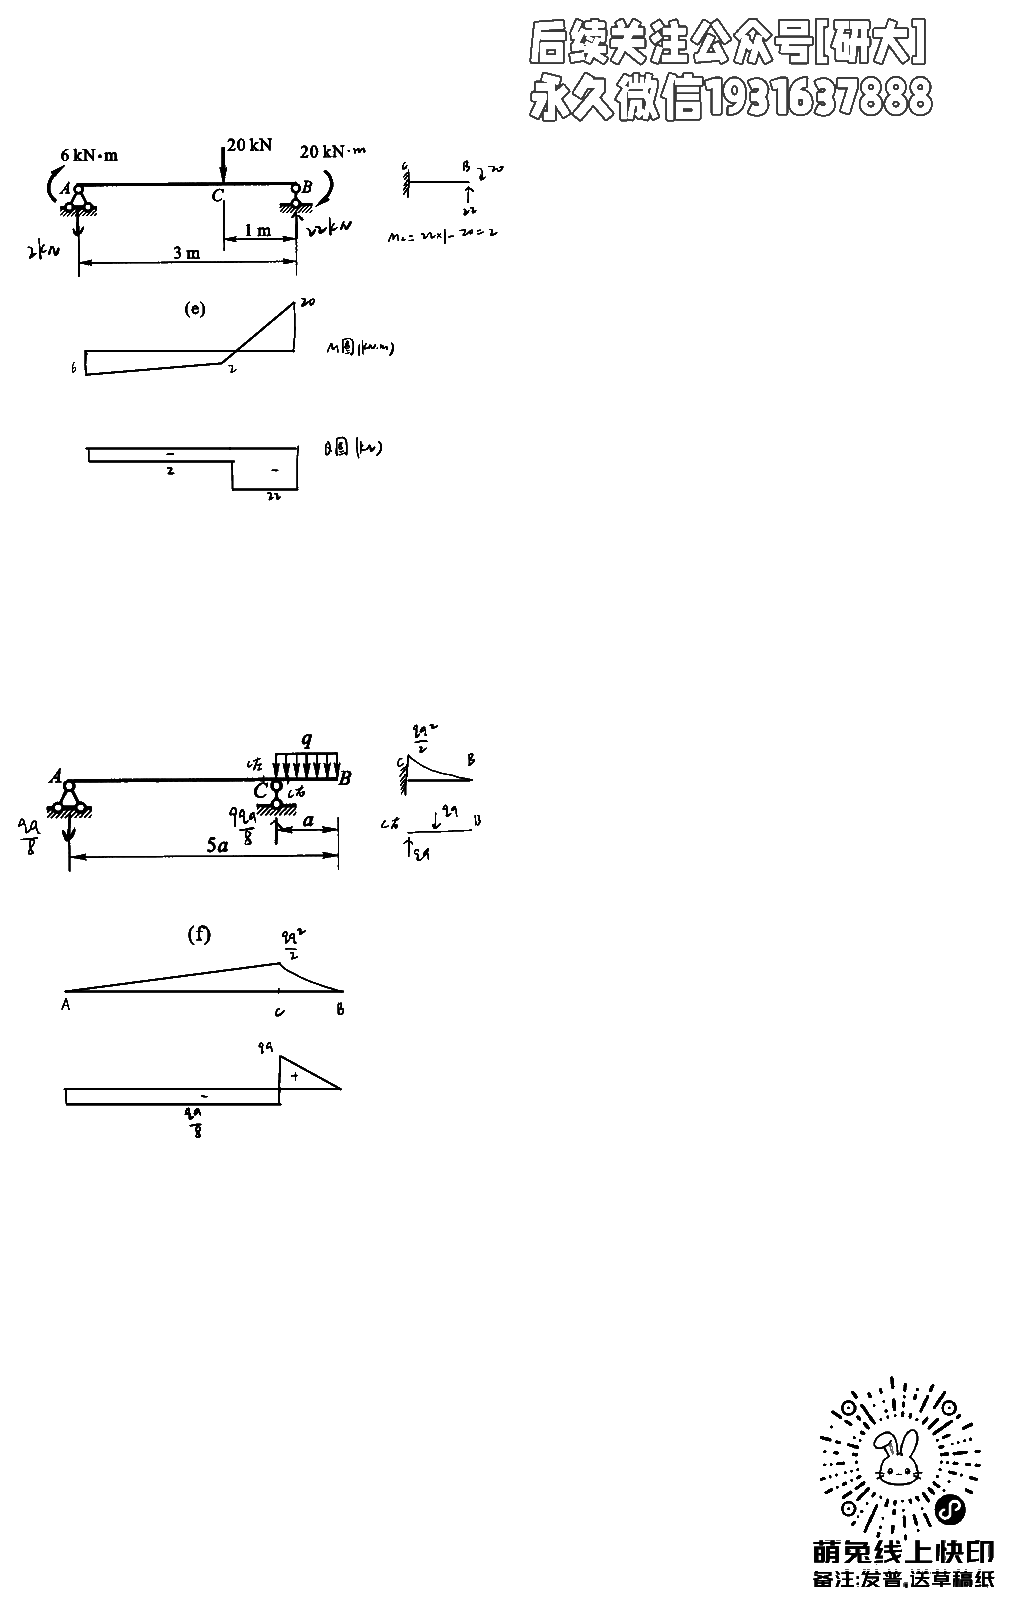
\includegraphics[width=0.96\textwidth,height=0.82\textheight,keepaspectratio]{images/c03_note_p03.png}
\par\small 讲解笔记（去水印版），第 3/9 页
\end{center}
\clearpage
\begin{center}
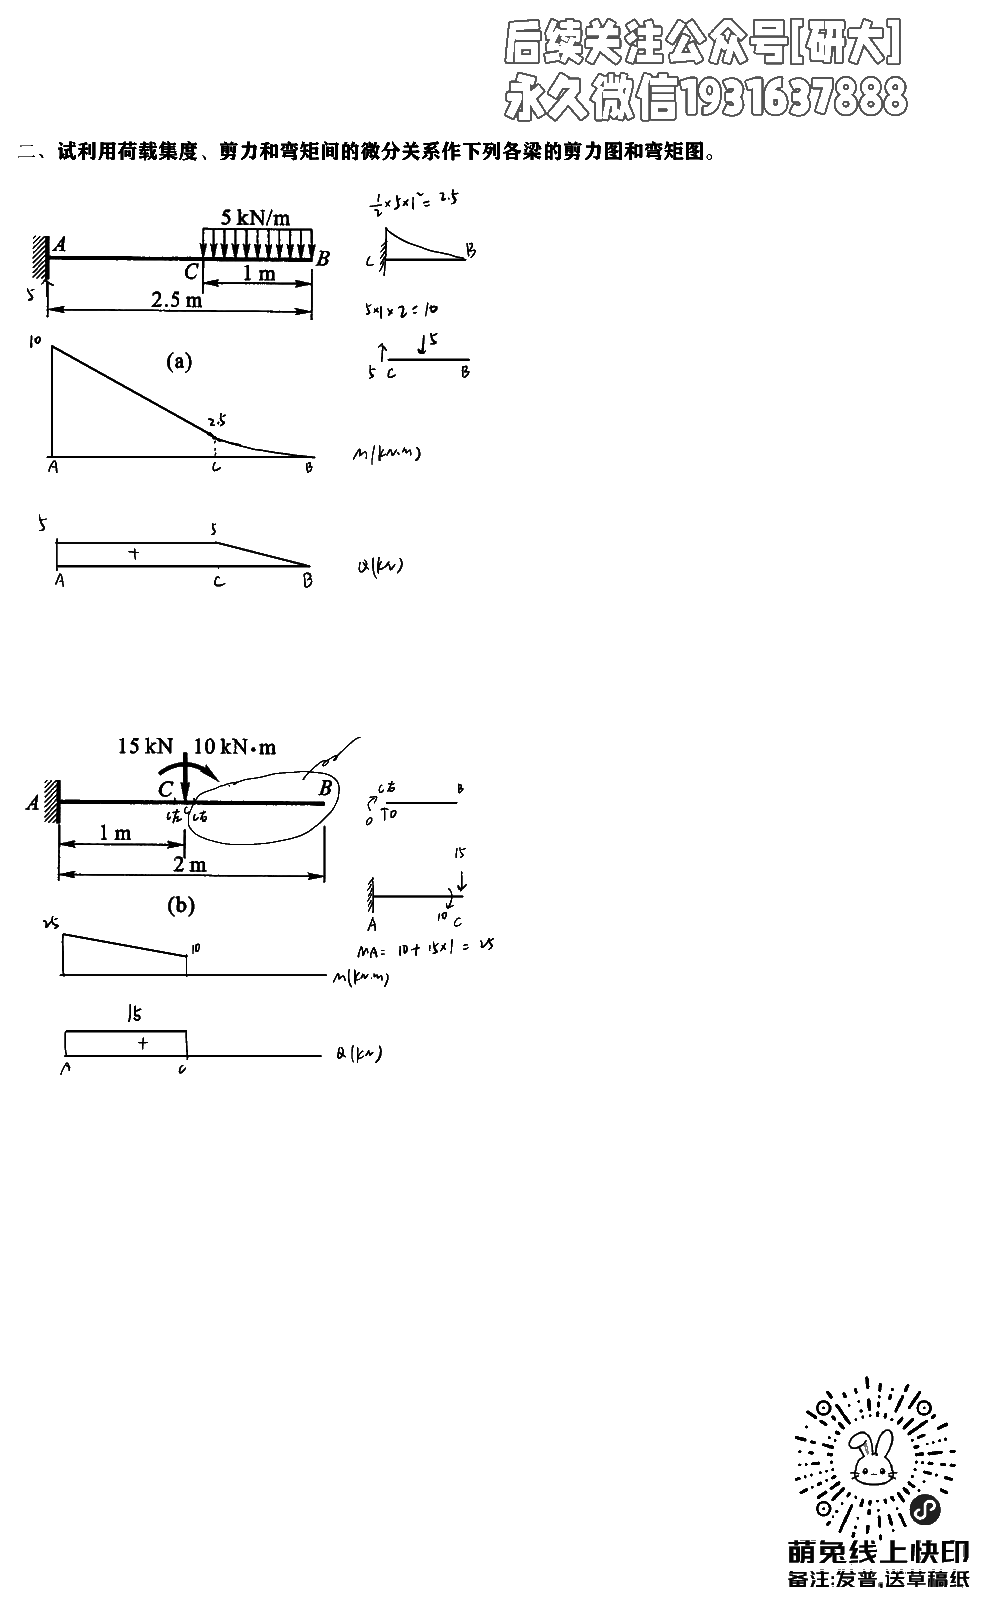
\includegraphics[width=0.96\textwidth,height=0.82\textheight,keepaspectratio]{images/c03_note_p04.png}
\par\small 讲解笔记（去水印版），第 4/9 页
\end{center}
\clearpage
\begin{center}
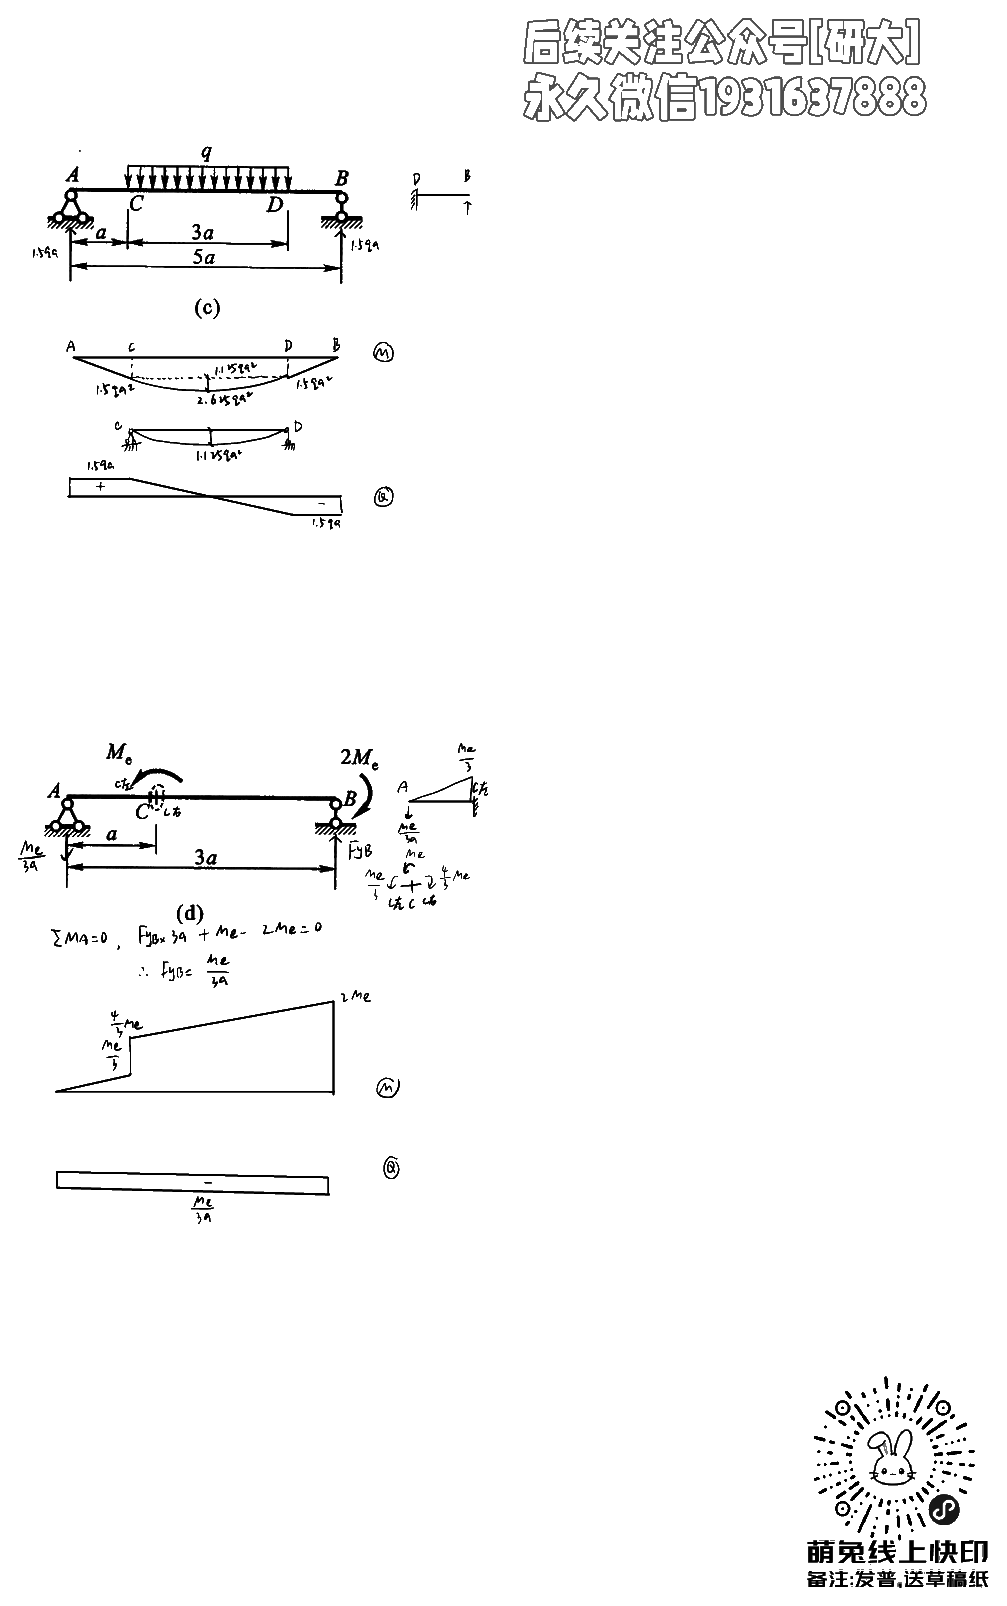
\includegraphics[width=0.96\textwidth,height=0.82\textheight,keepaspectratio]{images/c03_note_p05.png}
\par\small 讲解笔记（去水印版），第 5/9 页
\end{center}
\clearpage
\begin{center}
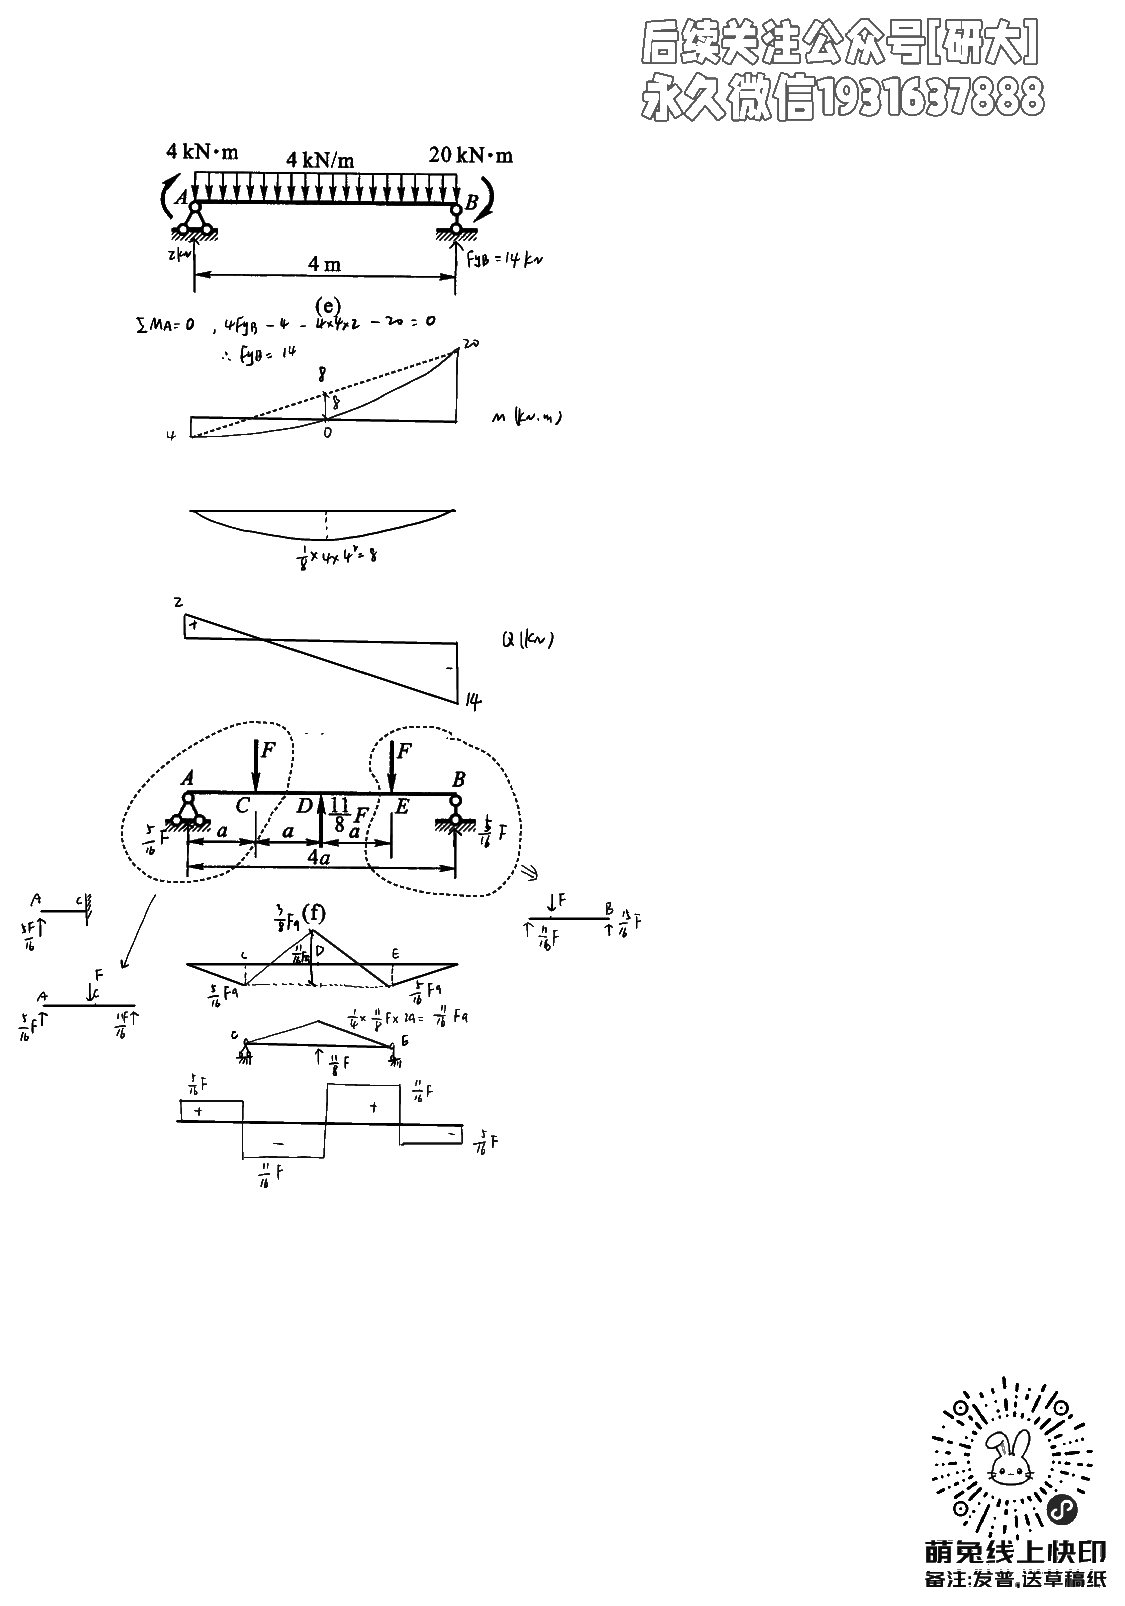
\includegraphics[width=0.96\textwidth,height=0.82\textheight,keepaspectratio]{images/c03_note_p06.png}
\par\small 讲解笔记（去水印版），第 6/9 页
\end{center}
\clearpage
\begin{center}
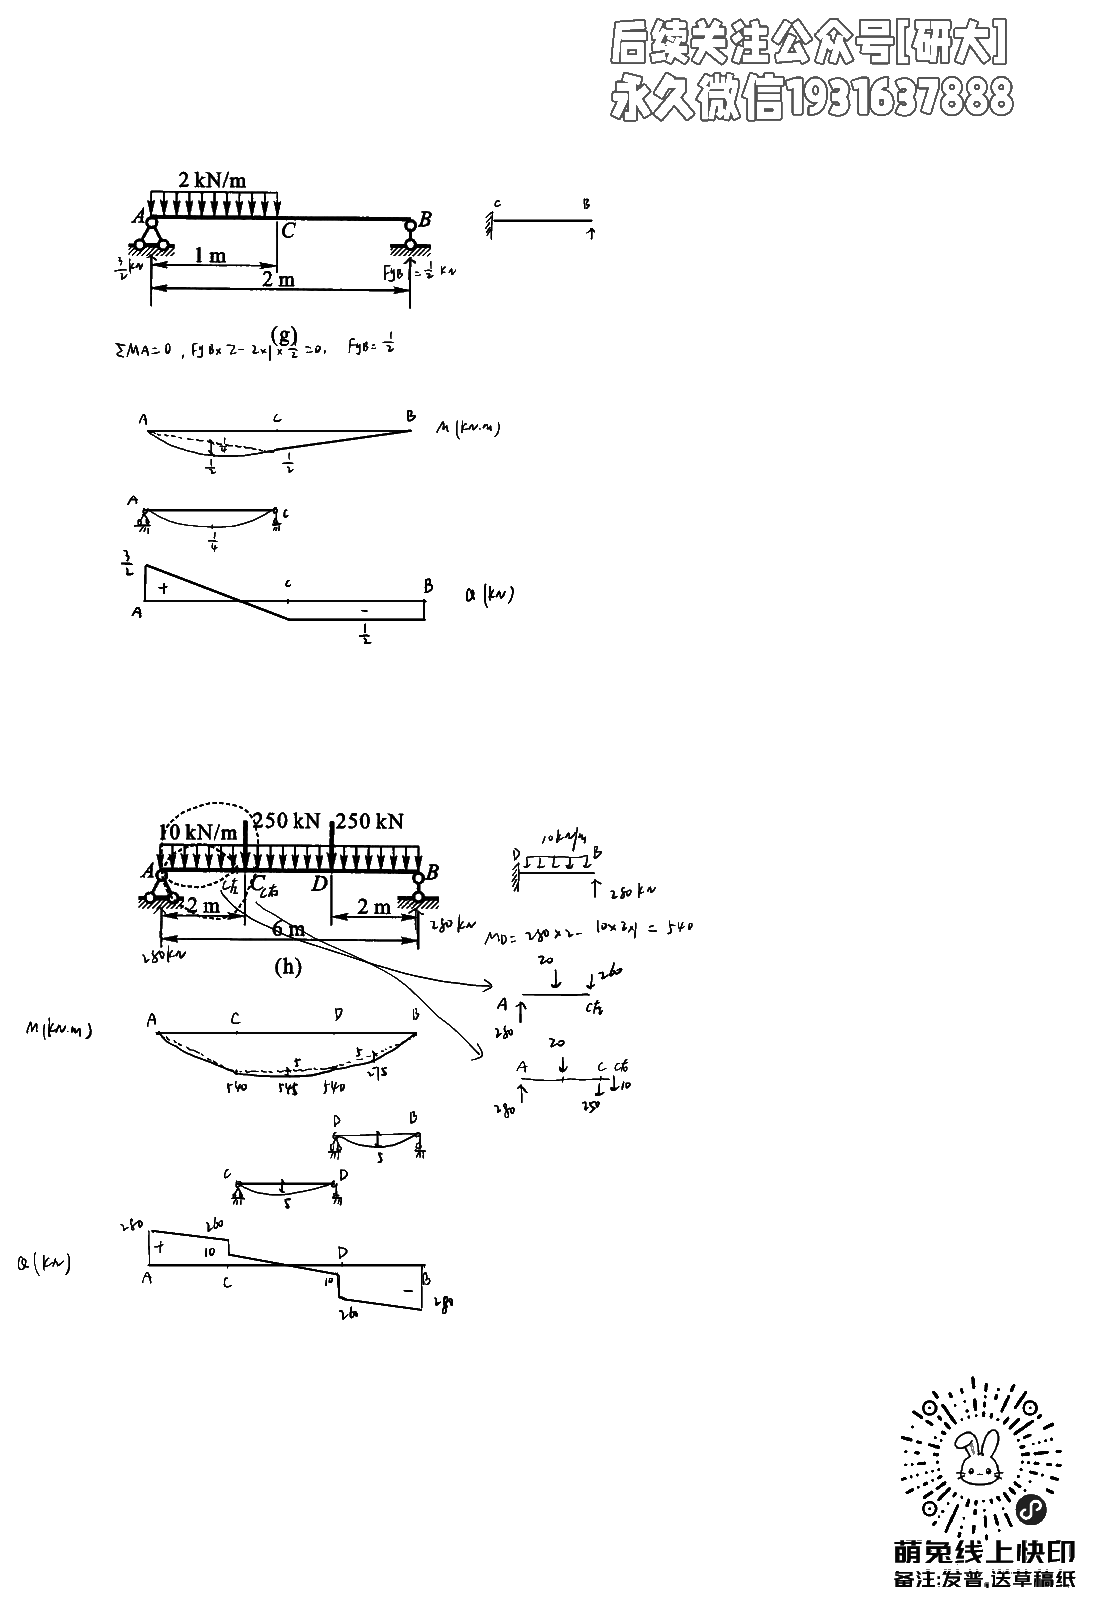
\includegraphics[width=0.96\textwidth,height=0.82\textheight,keepaspectratio]{images/c03_note_p07.png}
\par\small 讲解笔记（去水印版），第 7/9 页
\end{center}
\clearpage
\begin{center}
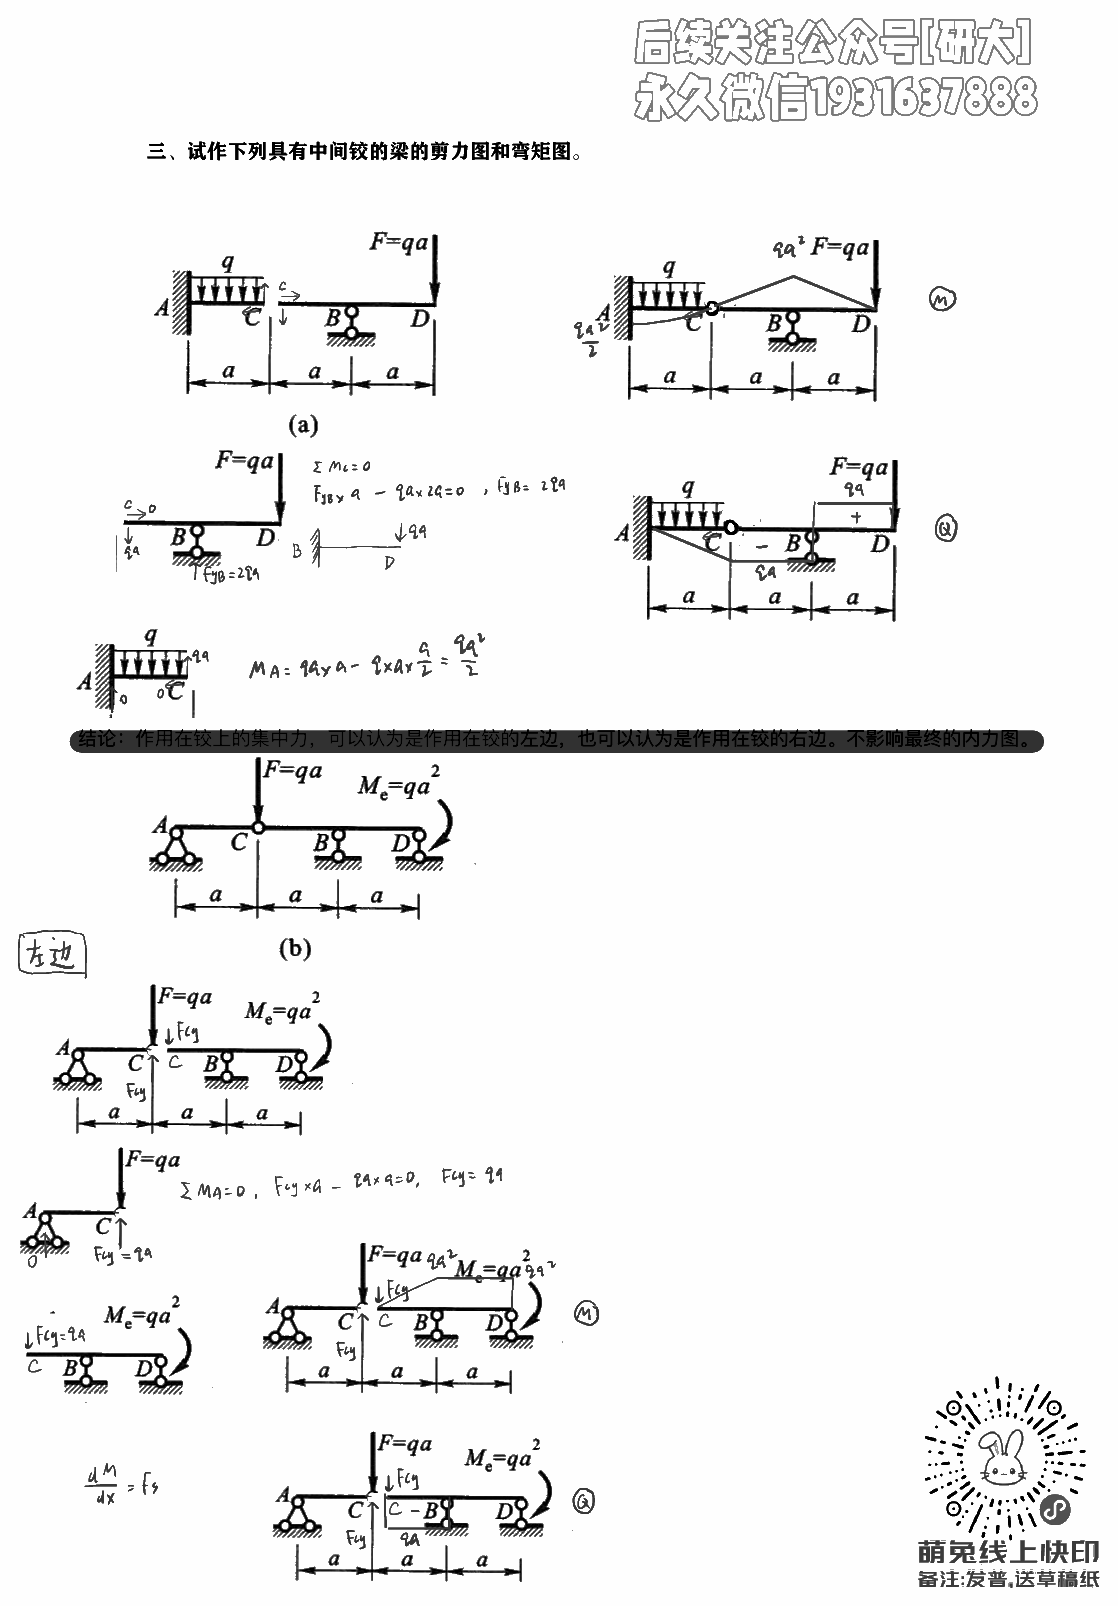
\includegraphics[width=0.96\textwidth,height=0.82\textheight,keepaspectratio]{images/c03_note_p08.png}
\par\small 讲解笔记（去水印版），第 8/9 页
\end{center}
\clearpage
\begin{center}
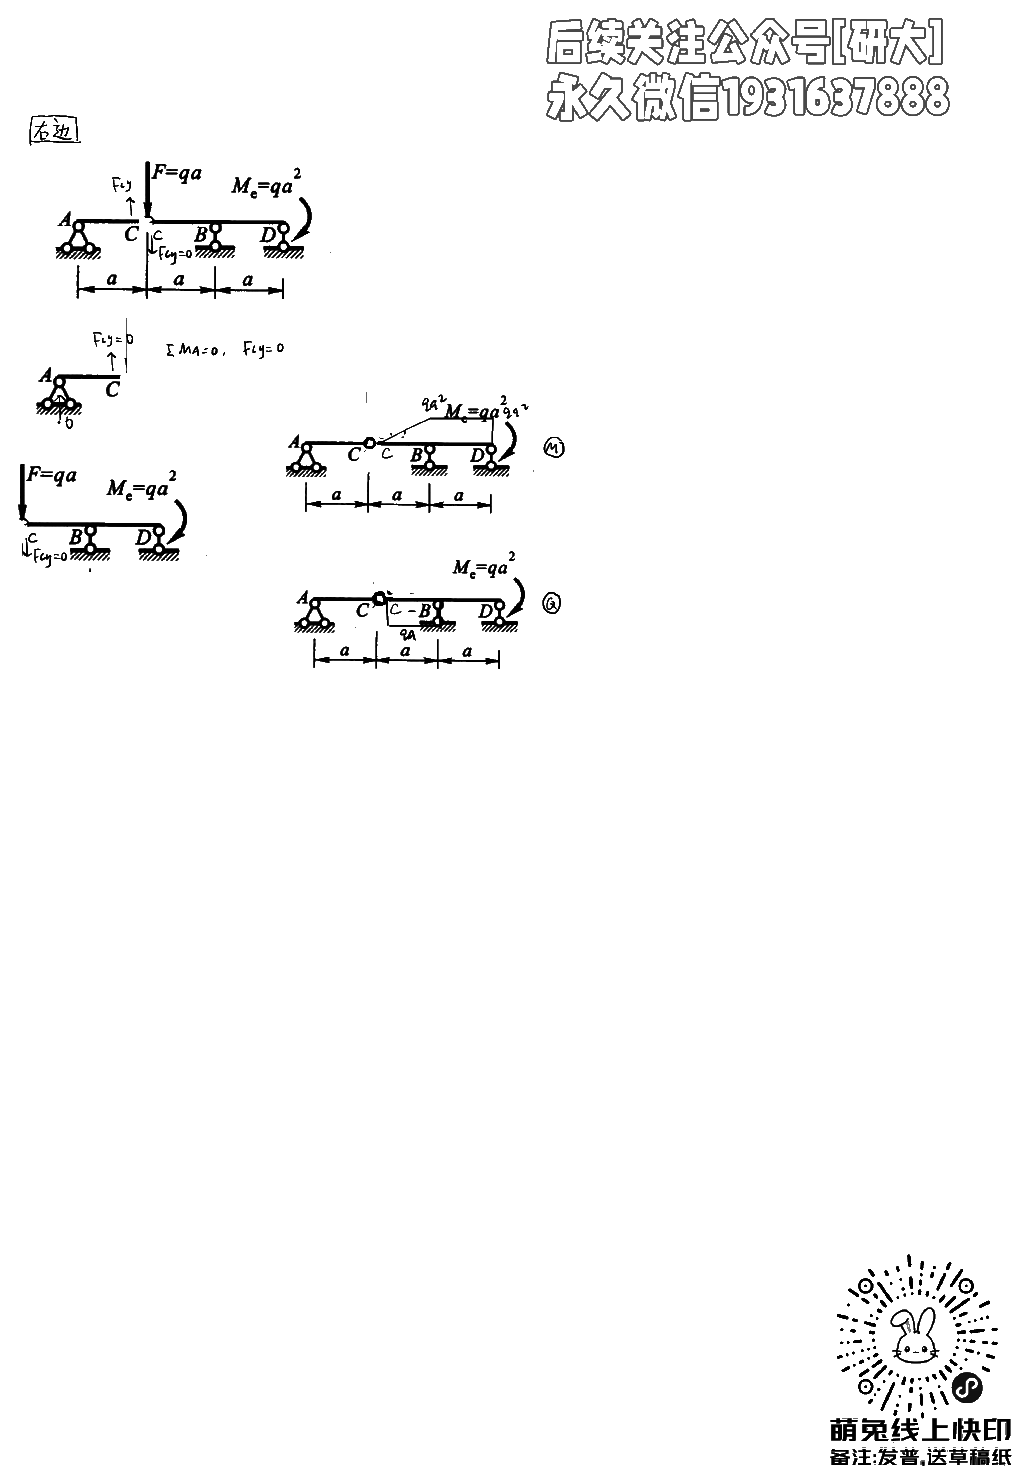
\includegraphics[width=0.96\textwidth,height=0.82\textheight,keepaspectratio]{images/c03_note_p09.png}
\par\small 讲解笔记（去水印版），第 9/9 页
\end{center}
\clearpage
\chapter{第4讲：静定梁和刚架}
\begin{tcolorbox}[title=解析要点]
静定梁和刚架先由整体平衡求支座反力，再分段求剪力、弯矩和轴力。内力图要用集中力、集中力偶、铰结点等位置的突变规律校核。
\end{tcolorbox}
\begin{tcolorbox}[title=答案与校核]
答案页包含静定梁与刚架内力图；关键截面的剪力、弯矩值可作为校核点。
\end{tcolorbox}
\section{作业与答案（去水印版）}
\begin{center}
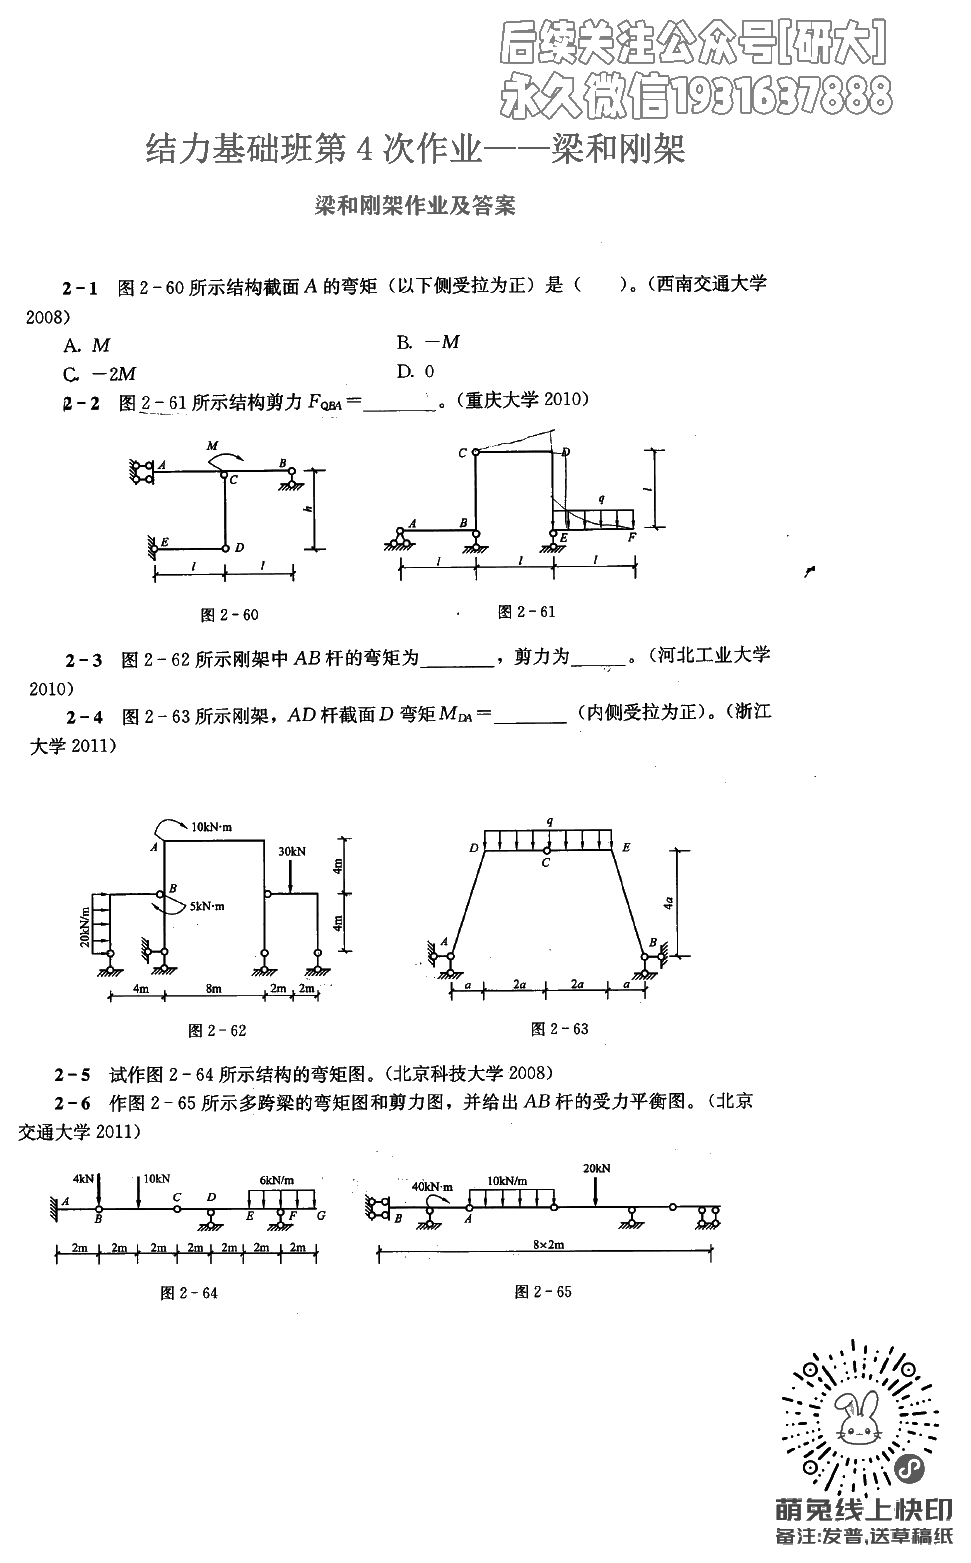
\includegraphics[width=0.96\textwidth,height=0.82\textheight,keepaspectratio]{images/c04_answer_1_p01.png}
\par\small 作业与答案（去水印版），第 1/14 页
\end{center}
\clearpage
\begin{center}
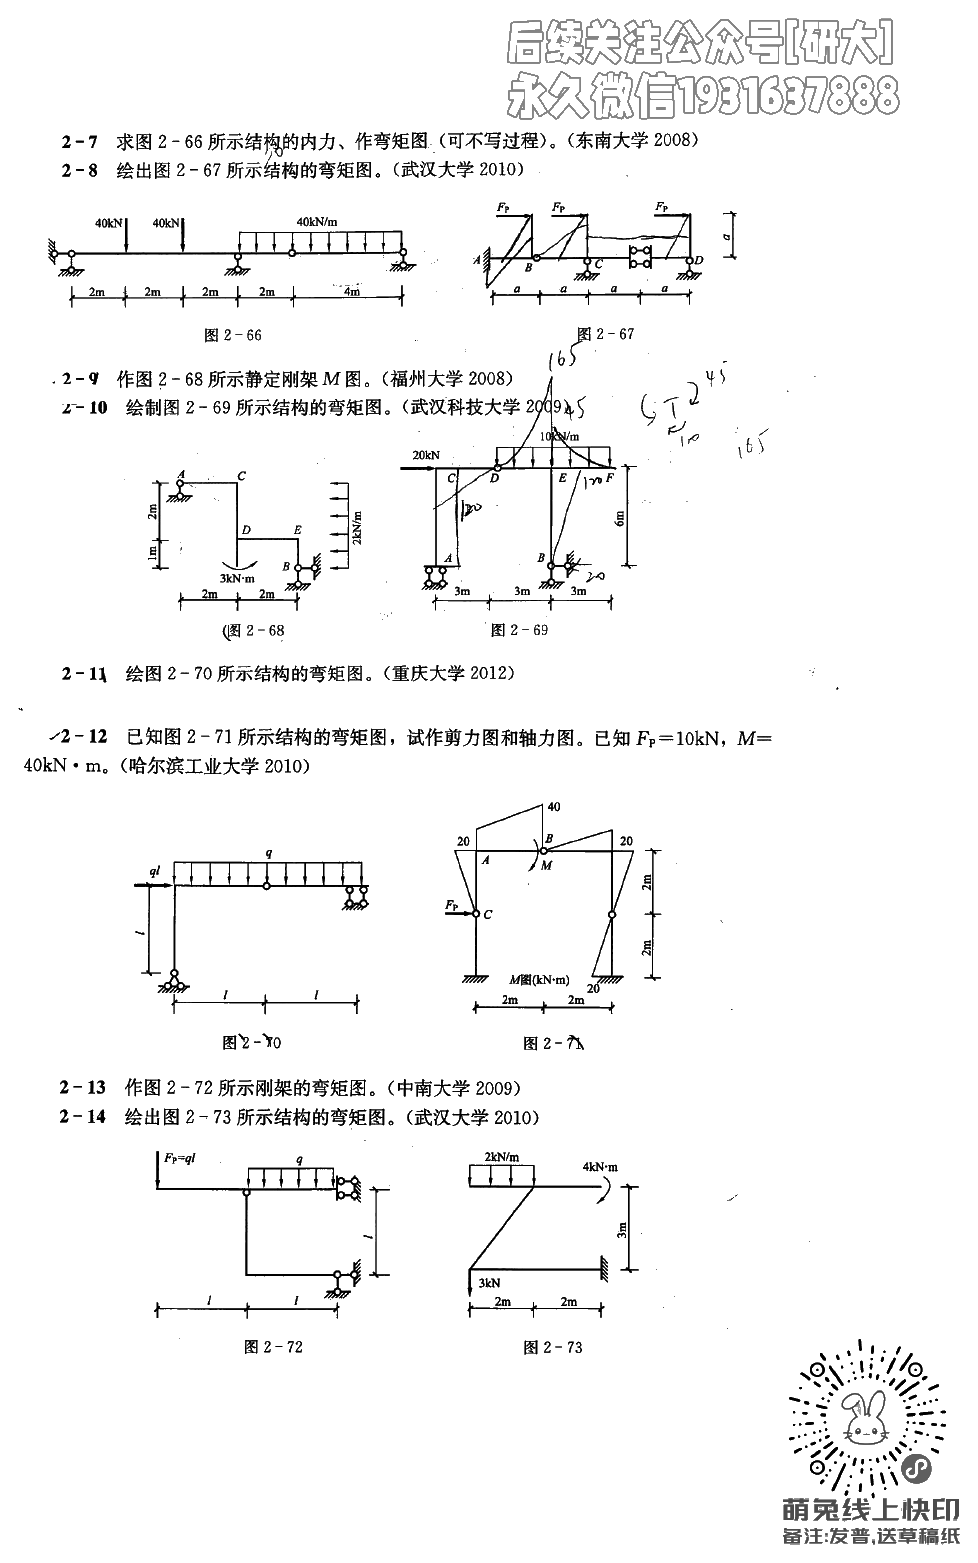
\includegraphics[width=0.96\textwidth,height=0.82\textheight,keepaspectratio]{images/c04_answer_1_p02.png}
\par\small 作业与答案（去水印版），第 2/14 页
\end{center}
\clearpage
\begin{center}
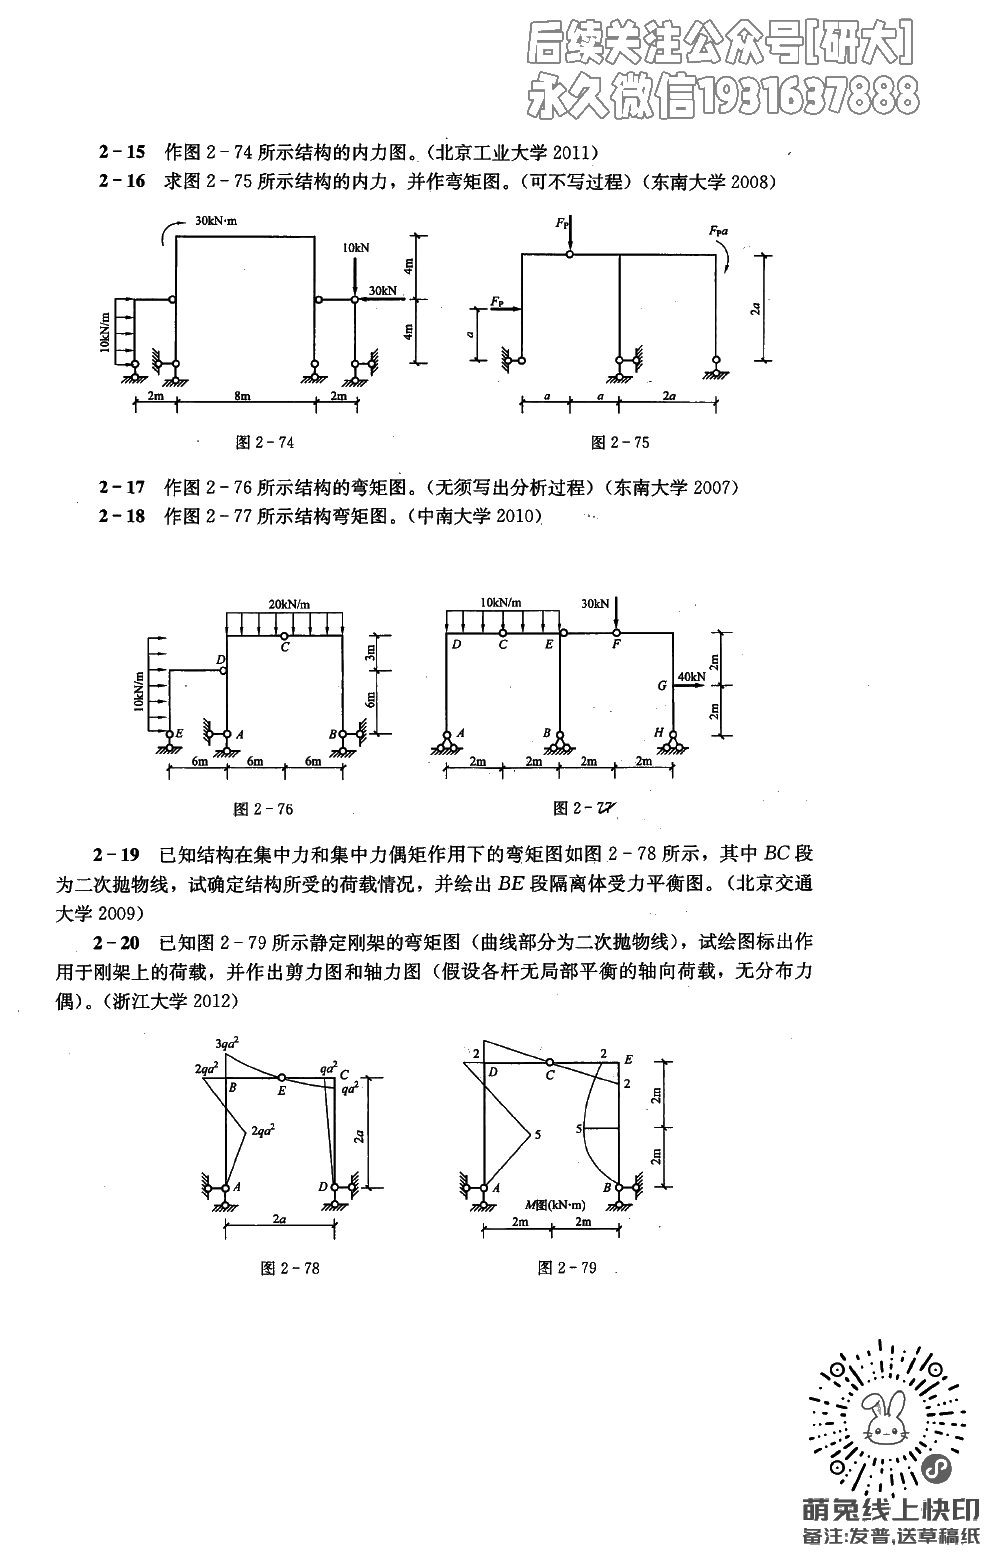
\includegraphics[width=0.96\textwidth,height=0.82\textheight,keepaspectratio]{images/c04_answer_1_p03.png}
\par\small 作业与答案（去水印版），第 3/14 页
\end{center}
\clearpage
\begin{center}
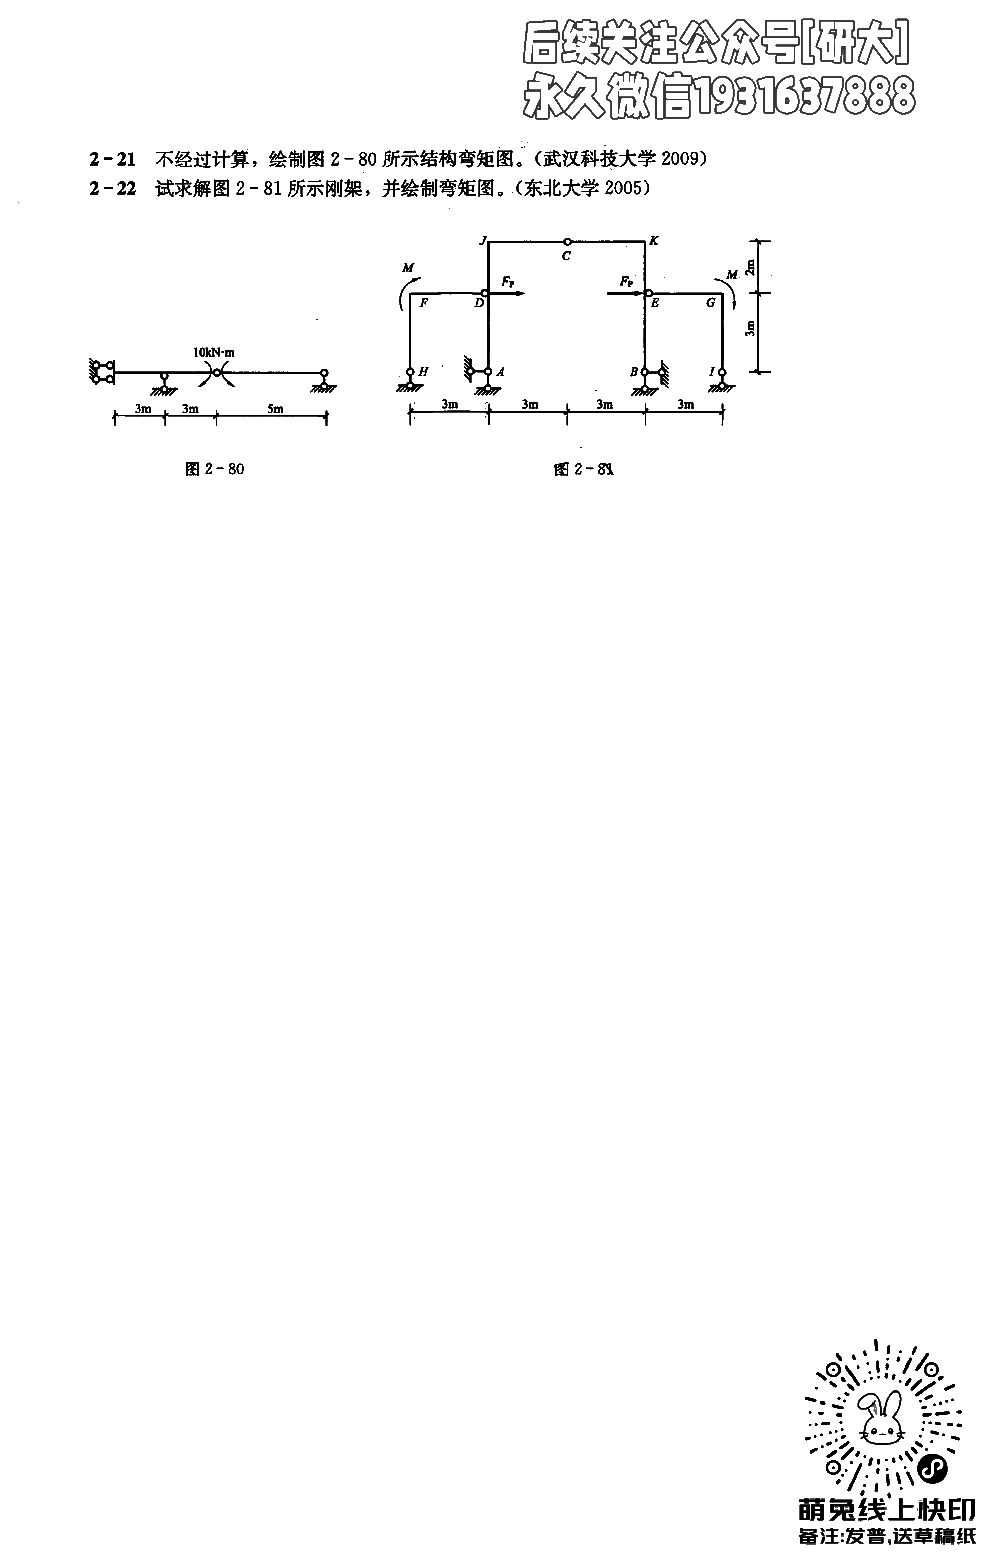
\includegraphics[width=0.96\textwidth,height=0.82\textheight,keepaspectratio]{images/c04_answer_1_p04.png}
\par\small 作业与答案（去水印版），第 4/14 页
\end{center}
\clearpage
\begin{center}
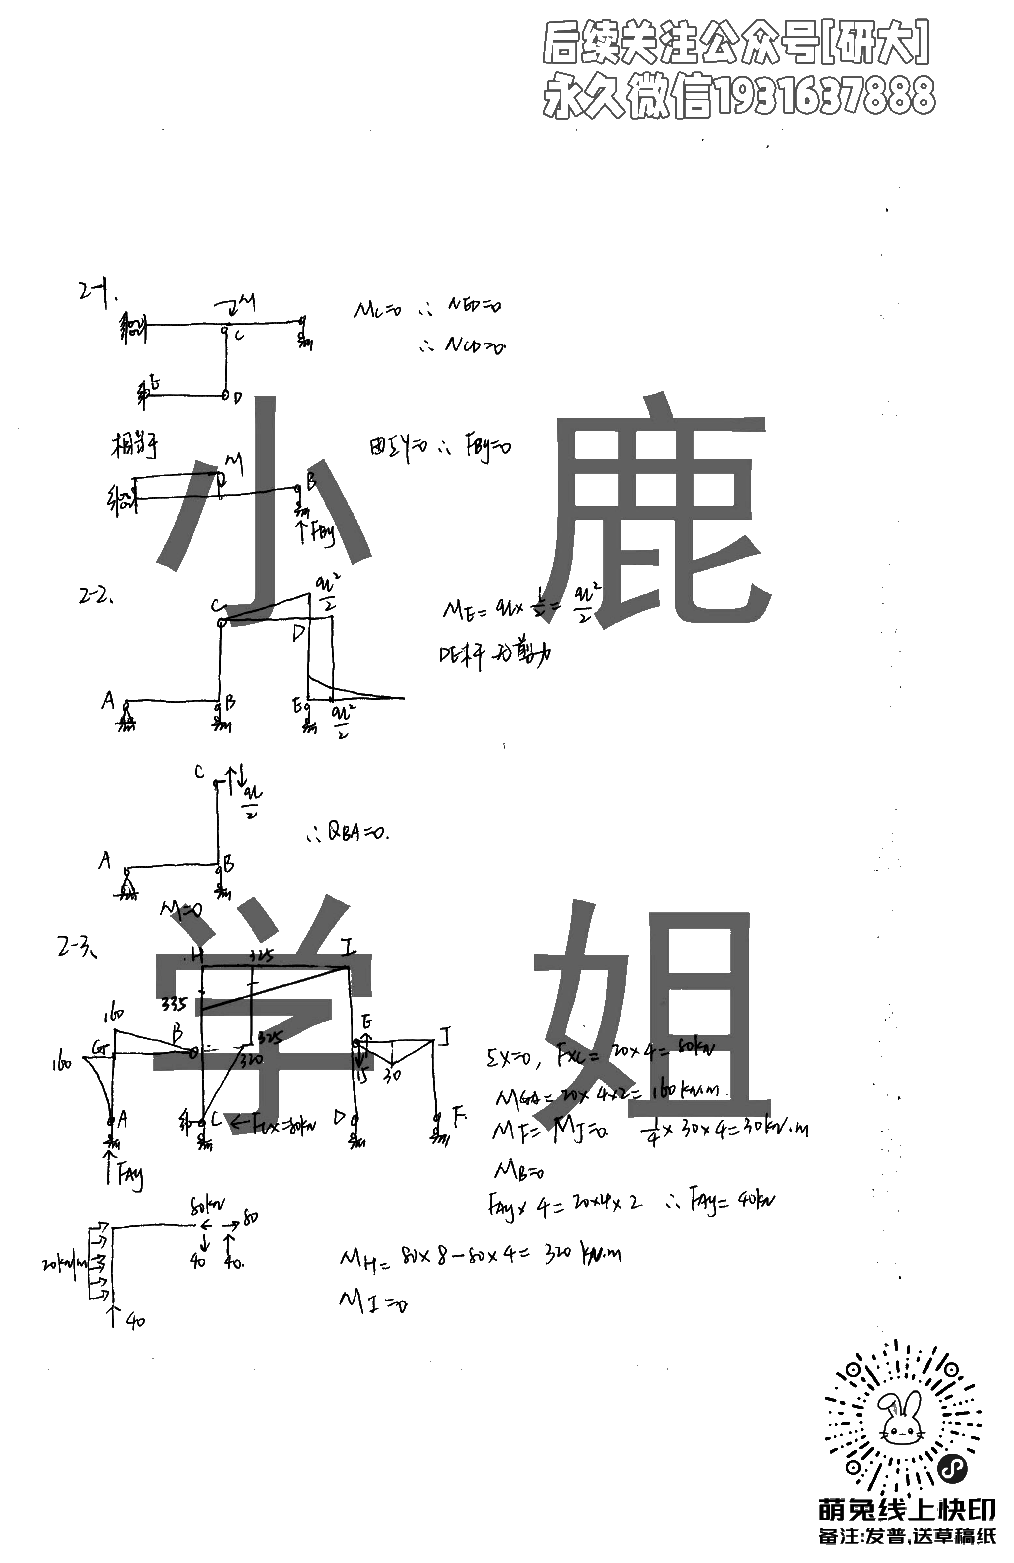
\includegraphics[width=0.96\textwidth,height=0.82\textheight,keepaspectratio]{images/c04_answer_1_p05.png}
\par\small 作业与答案（去水印版），第 5/14 页
\end{center}
\clearpage
\begin{center}
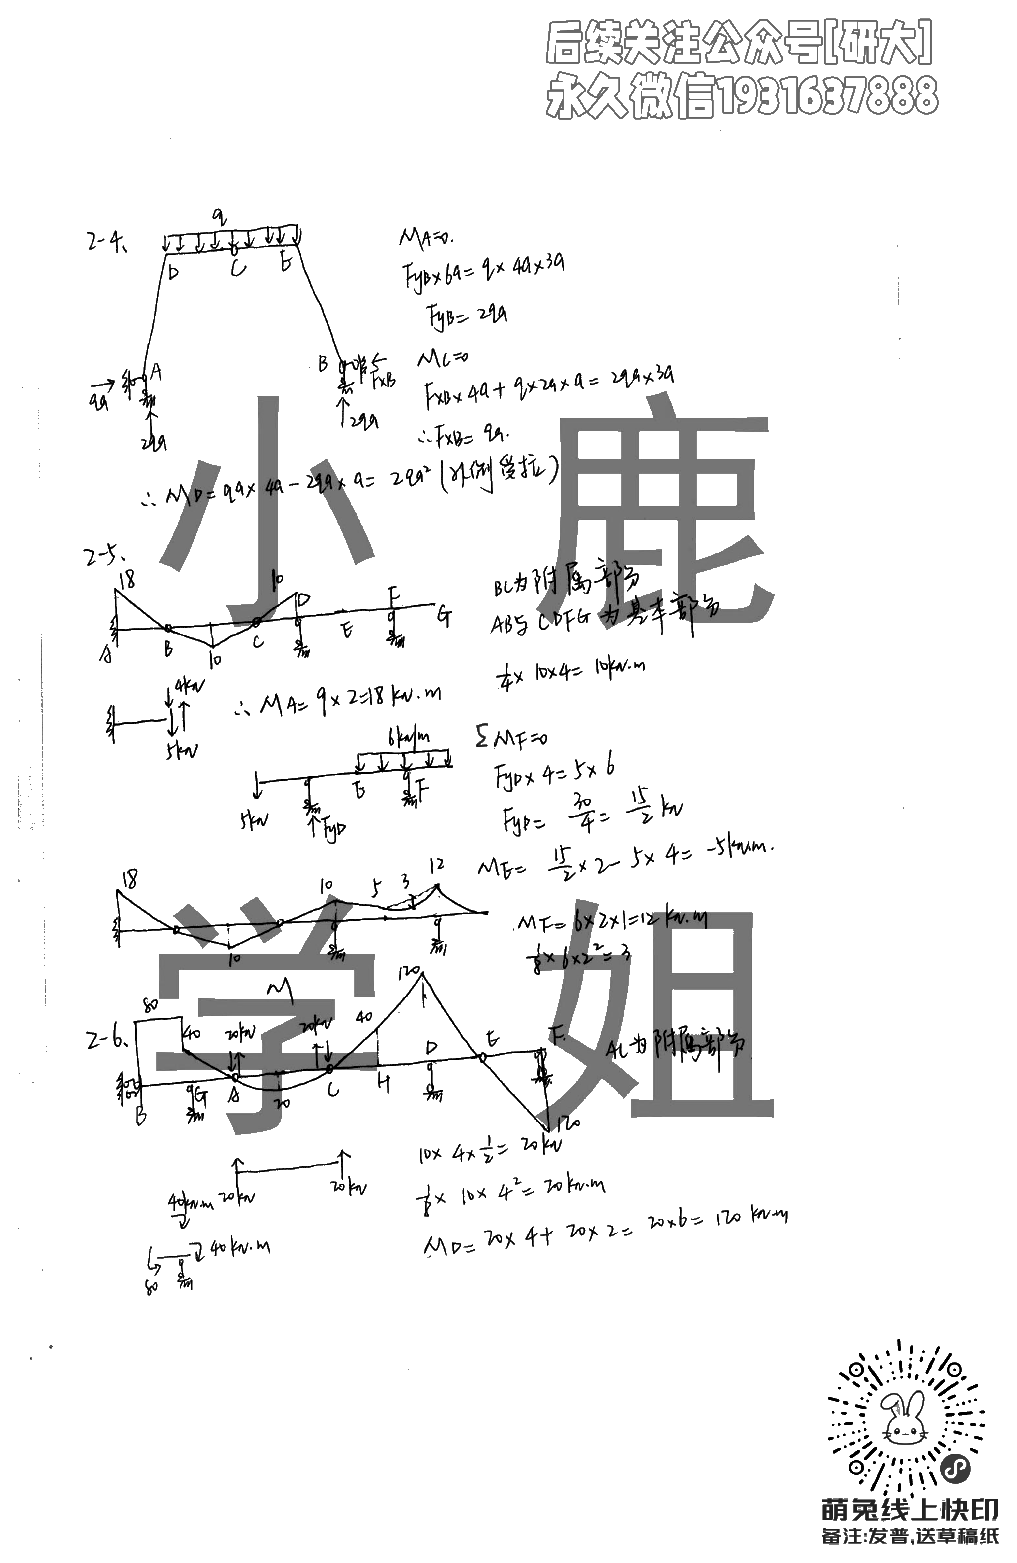
\includegraphics[width=0.96\textwidth,height=0.82\textheight,keepaspectratio]{images/c04_answer_1_p06.png}
\par\small 作业与答案（去水印版），第 6/14 页
\end{center}
\clearpage
\begin{center}
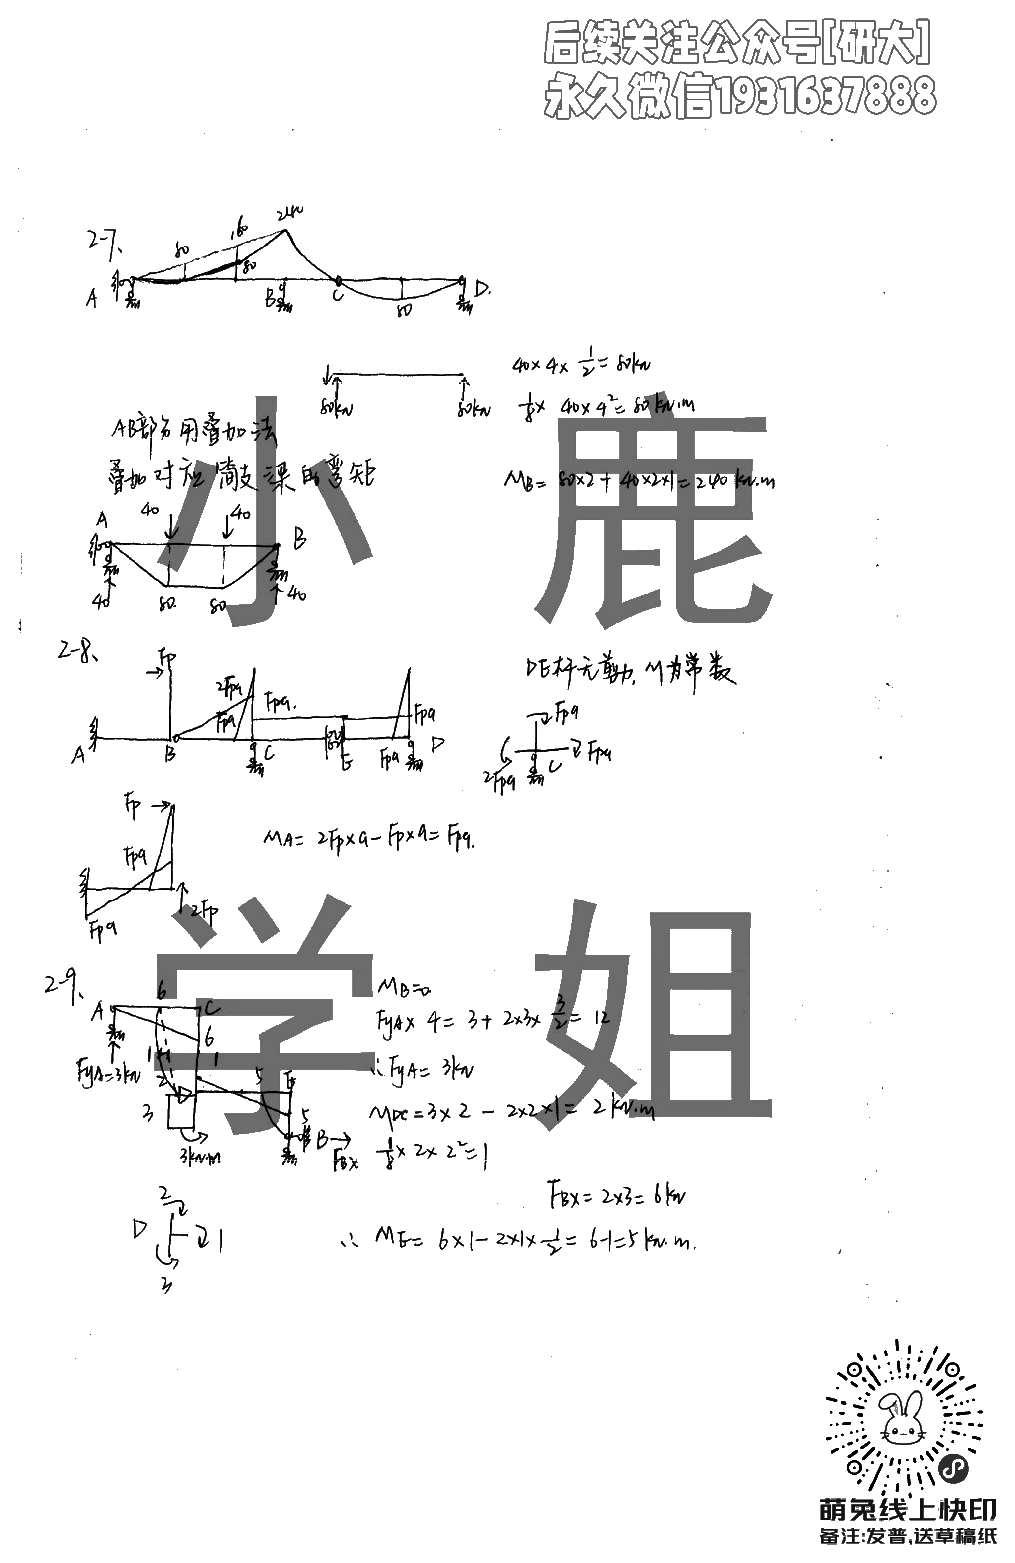
\includegraphics[width=0.96\textwidth,height=0.82\textheight,keepaspectratio]{images/c04_answer_1_p07.png}
\par\small 作业与答案（去水印版），第 7/14 页
\end{center}
\clearpage
\begin{center}
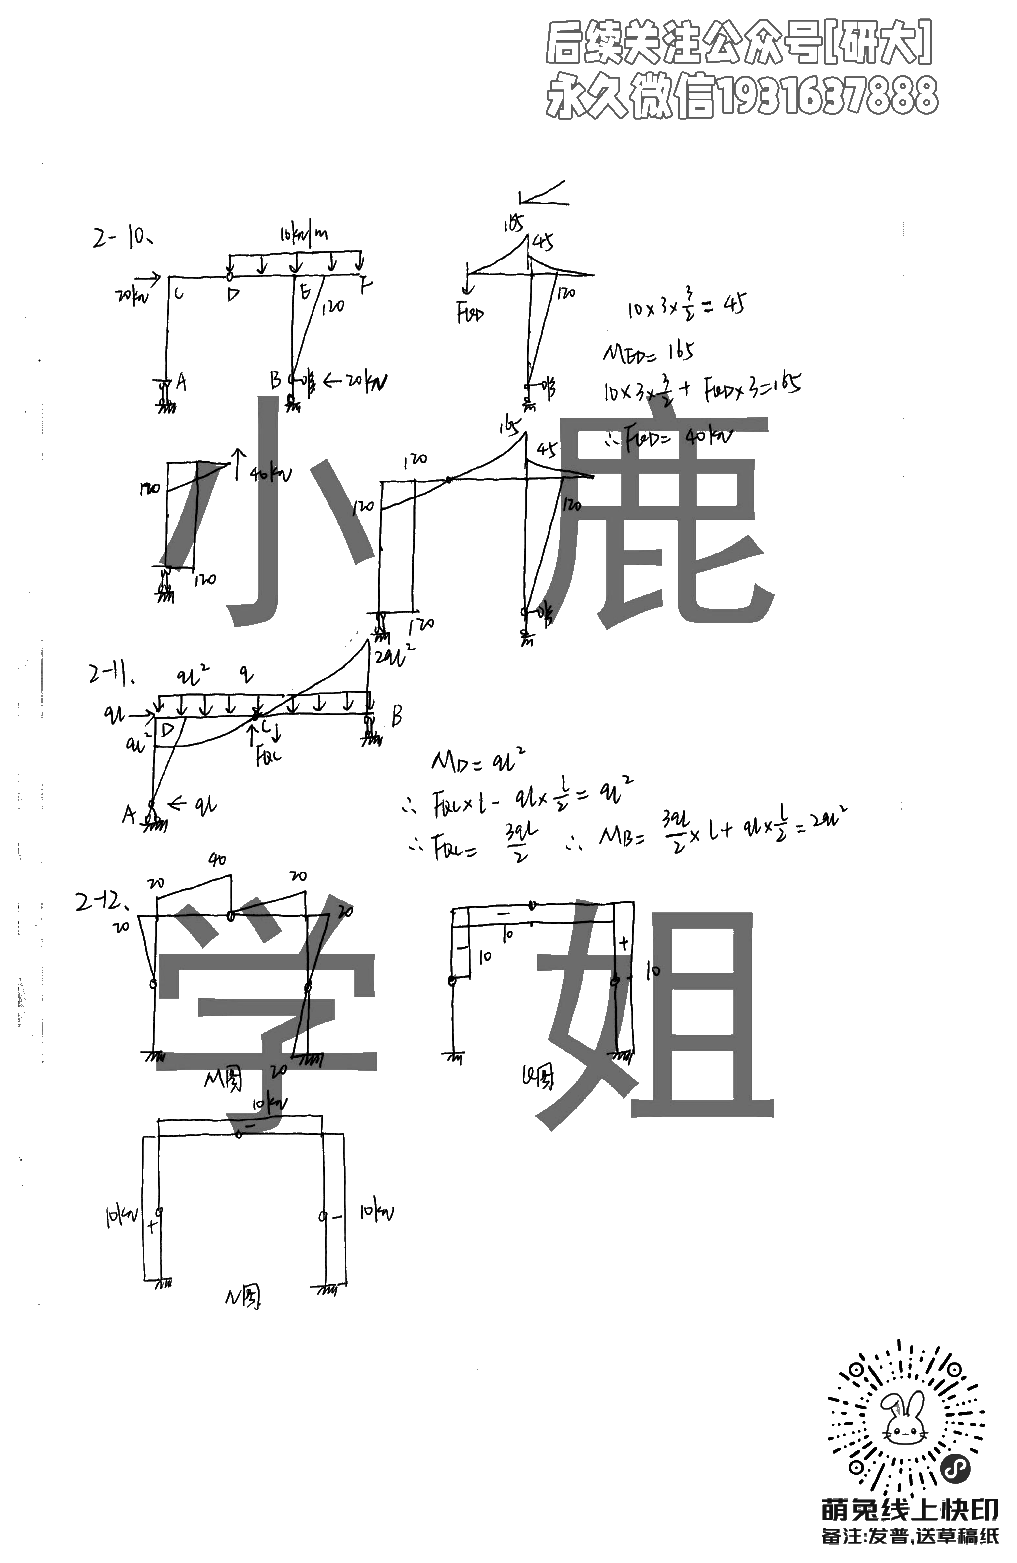
\includegraphics[width=0.96\textwidth,height=0.82\textheight,keepaspectratio]{images/c04_answer_1_p08.png}
\par\small 作业与答案（去水印版），第 8/14 页
\end{center}
\clearpage
\begin{center}
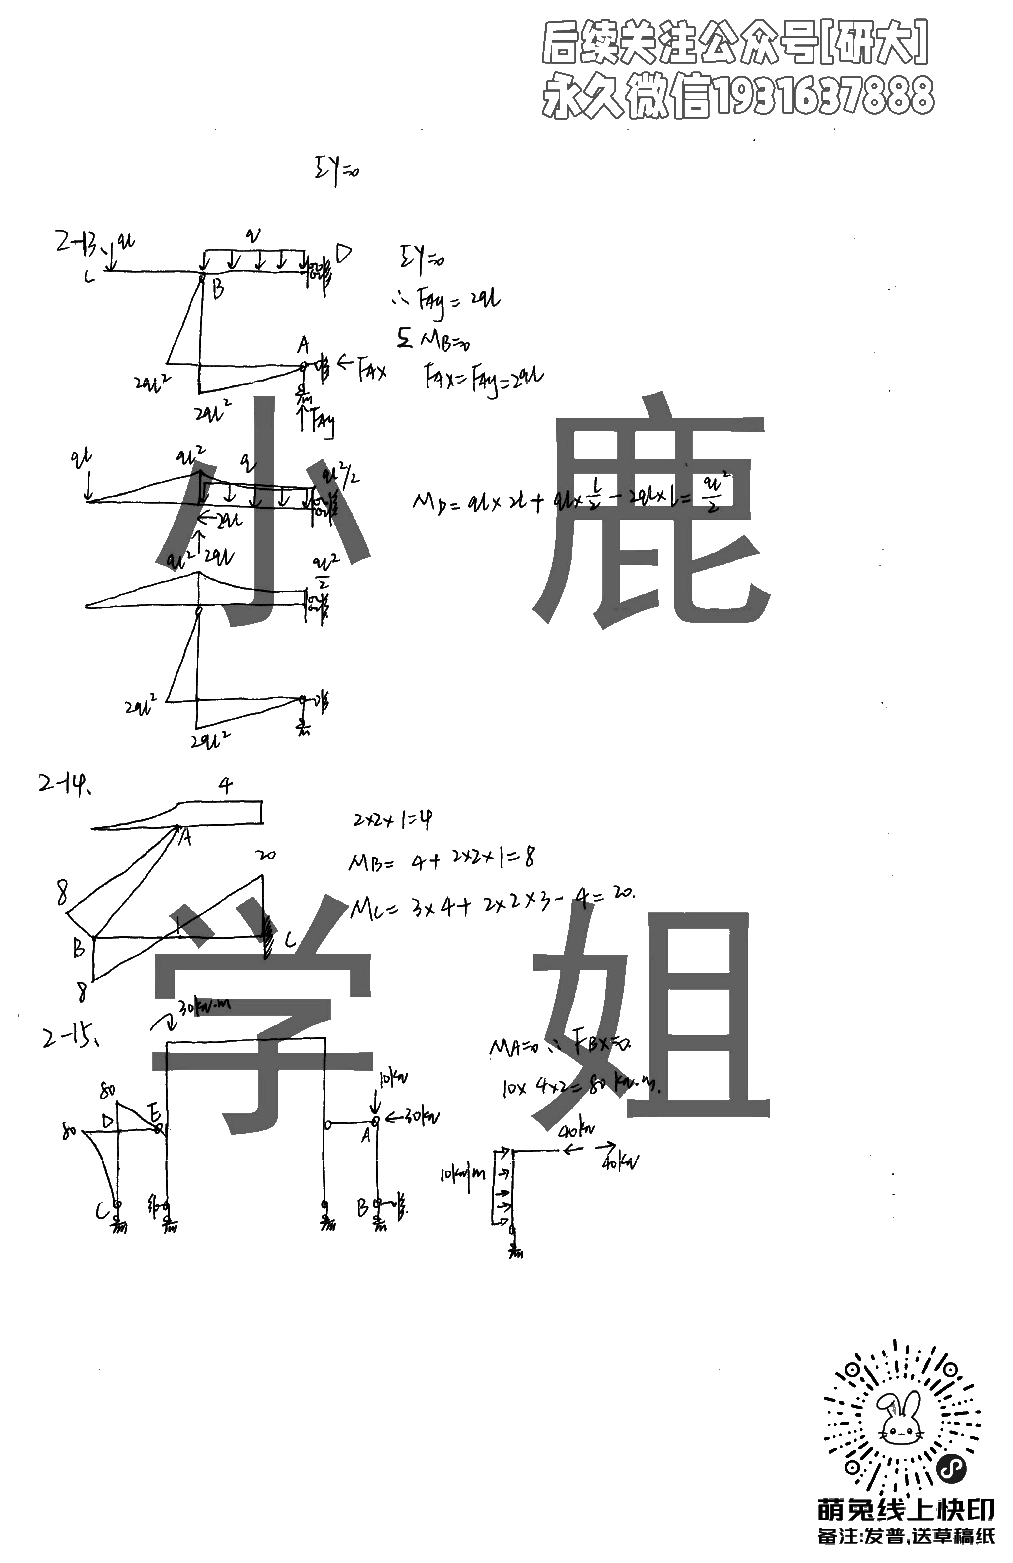
\includegraphics[width=0.96\textwidth,height=0.82\textheight,keepaspectratio]{images/c04_answer_1_p09.png}
\par\small 作业与答案（去水印版），第 9/14 页
\end{center}
\clearpage
\begin{center}
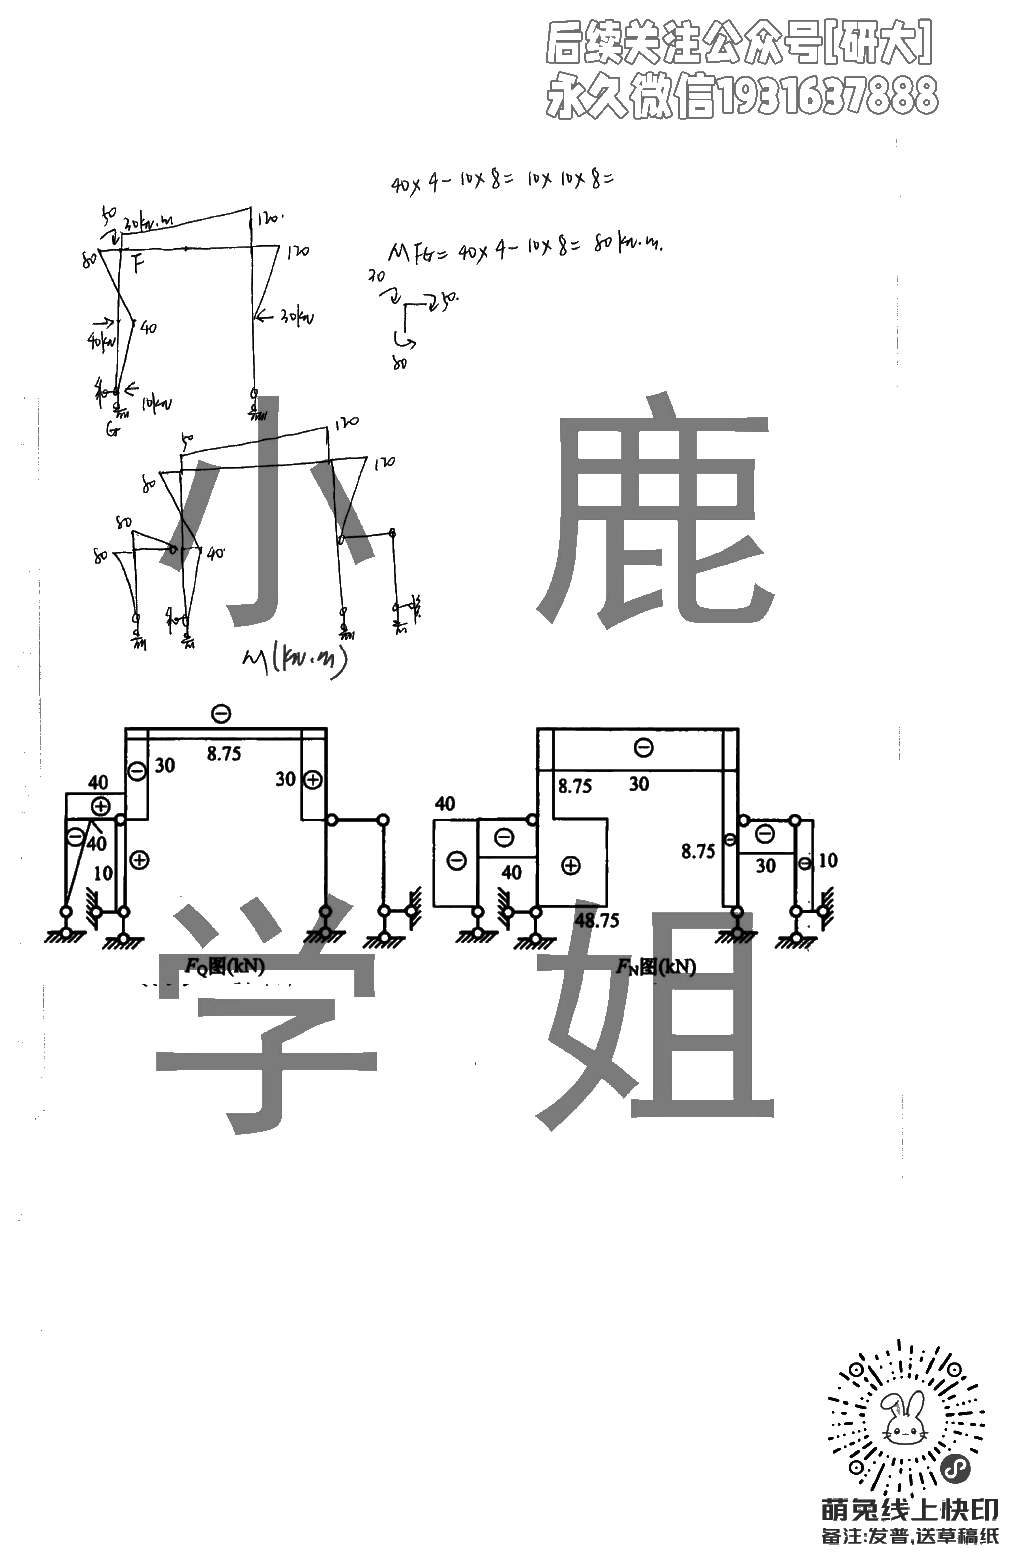
\includegraphics[width=0.96\textwidth,height=0.82\textheight,keepaspectratio]{images/c04_answer_1_p10.png}
\par\small 作业与答案（去水印版），第 10/14 页
\end{center}
\clearpage
\begin{center}
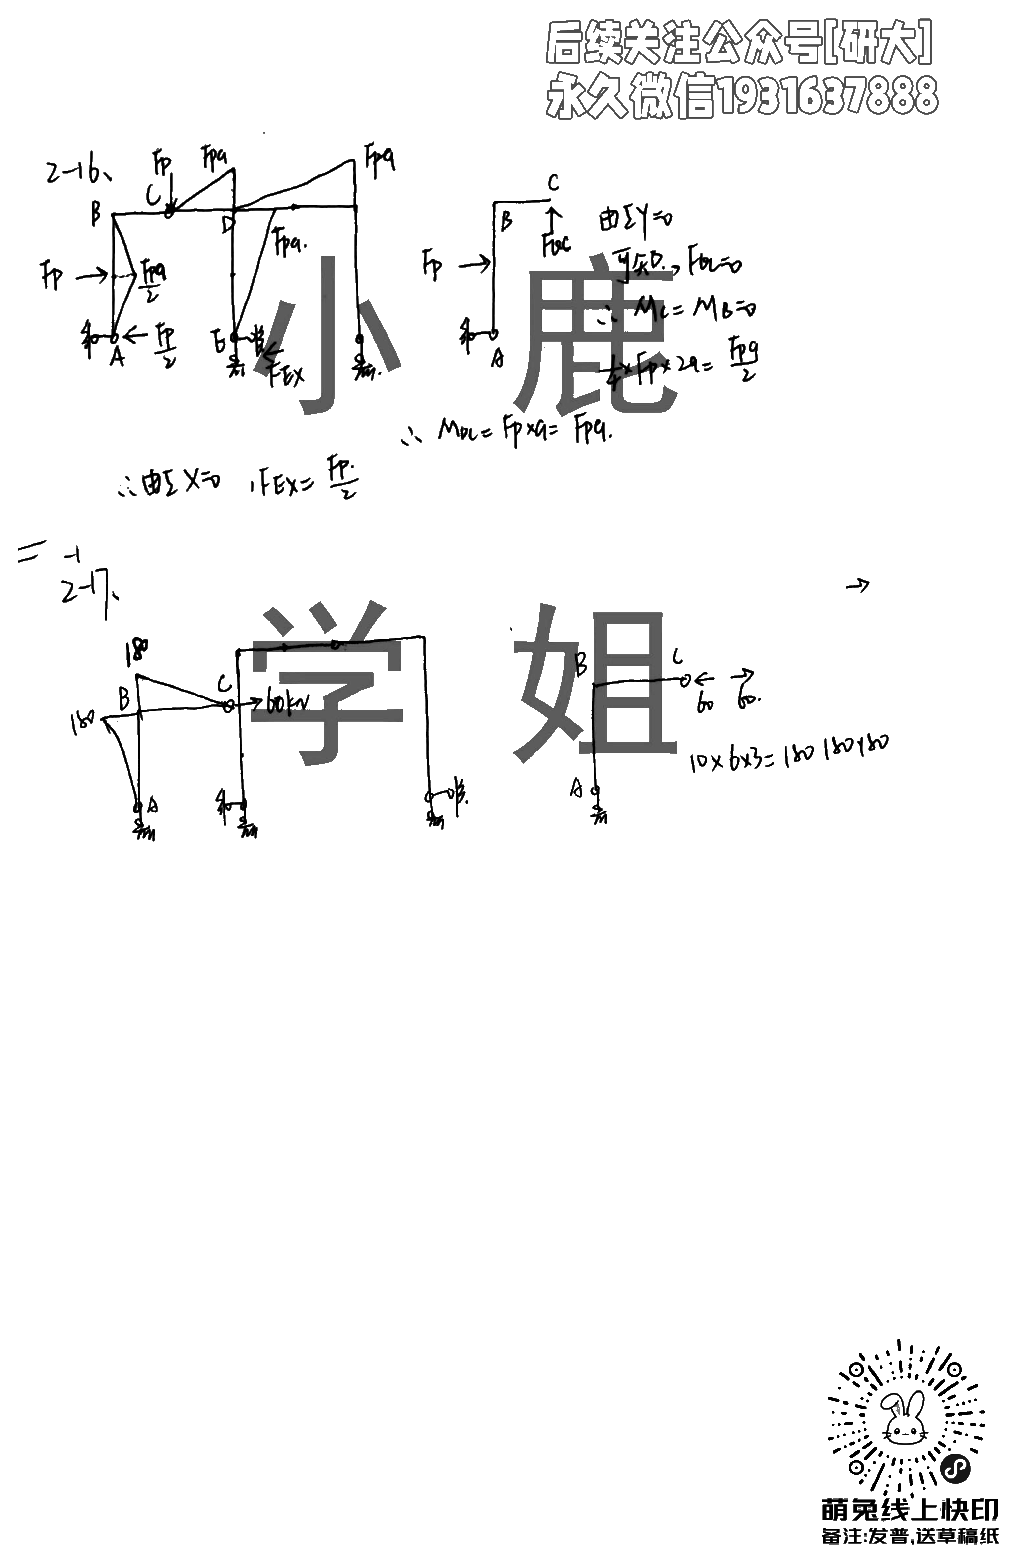
\includegraphics[width=0.96\textwidth,height=0.82\textheight,keepaspectratio]{images/c04_answer_1_p11.png}
\par\small 作业与答案（去水印版），第 11/14 页
\end{center}
\clearpage
\begin{center}
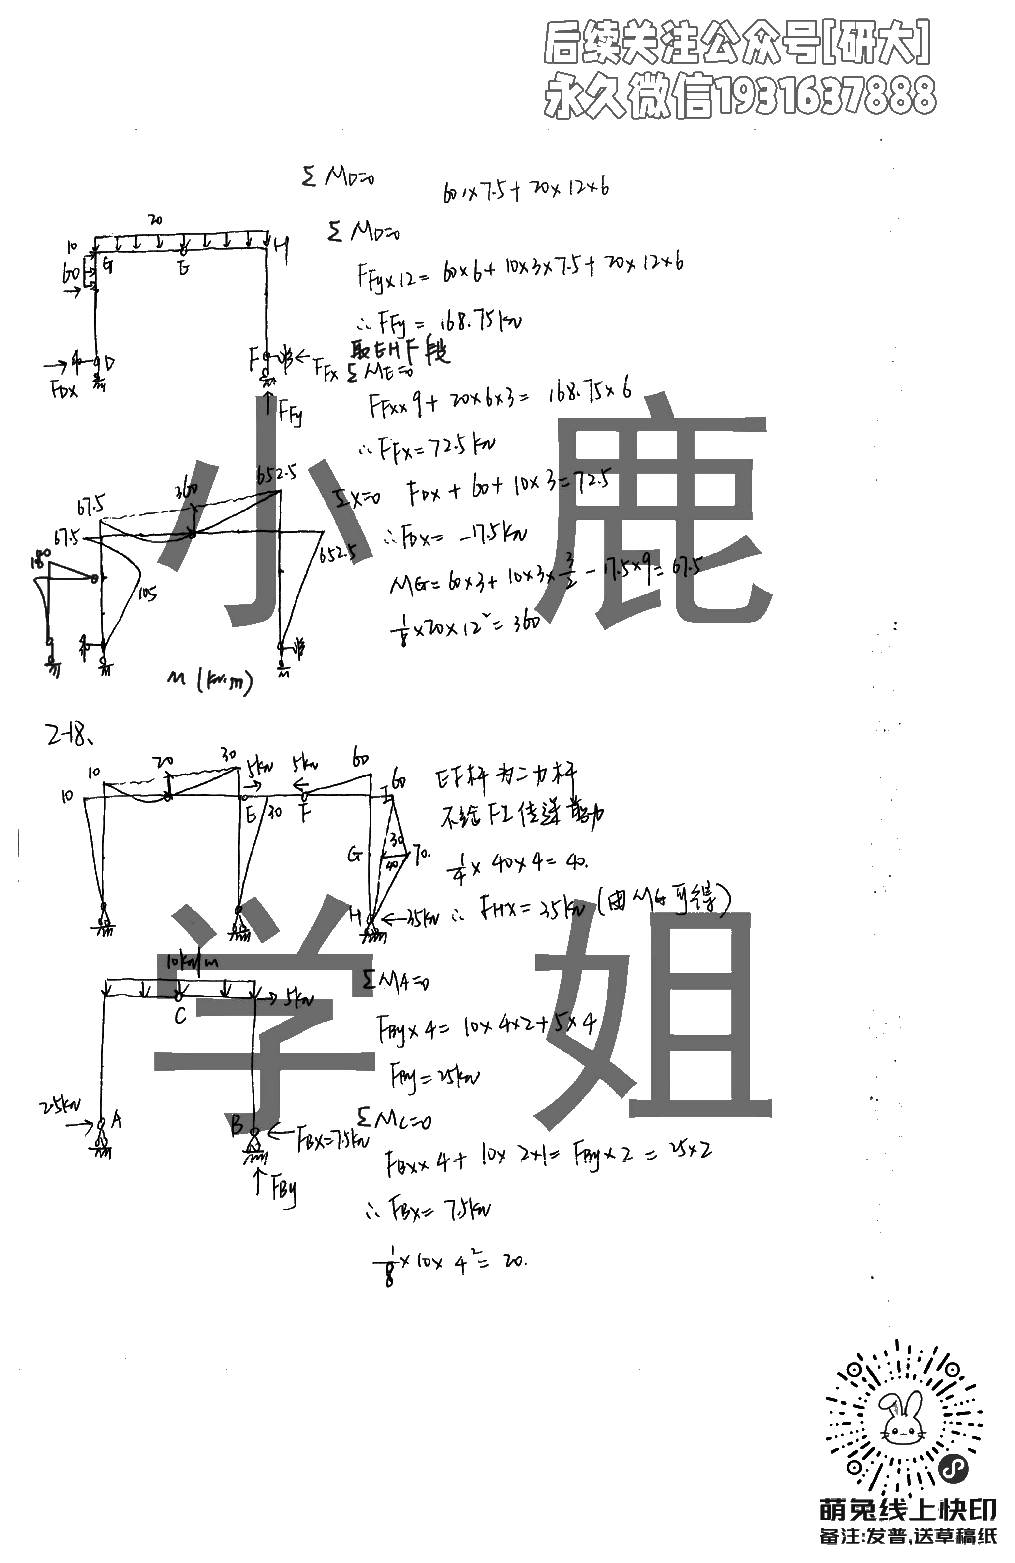
\includegraphics[width=0.96\textwidth,height=0.82\textheight,keepaspectratio]{images/c04_answer_1_p12.png}
\par\small 作业与答案（去水印版），第 12/14 页
\end{center}
\clearpage
\begin{center}
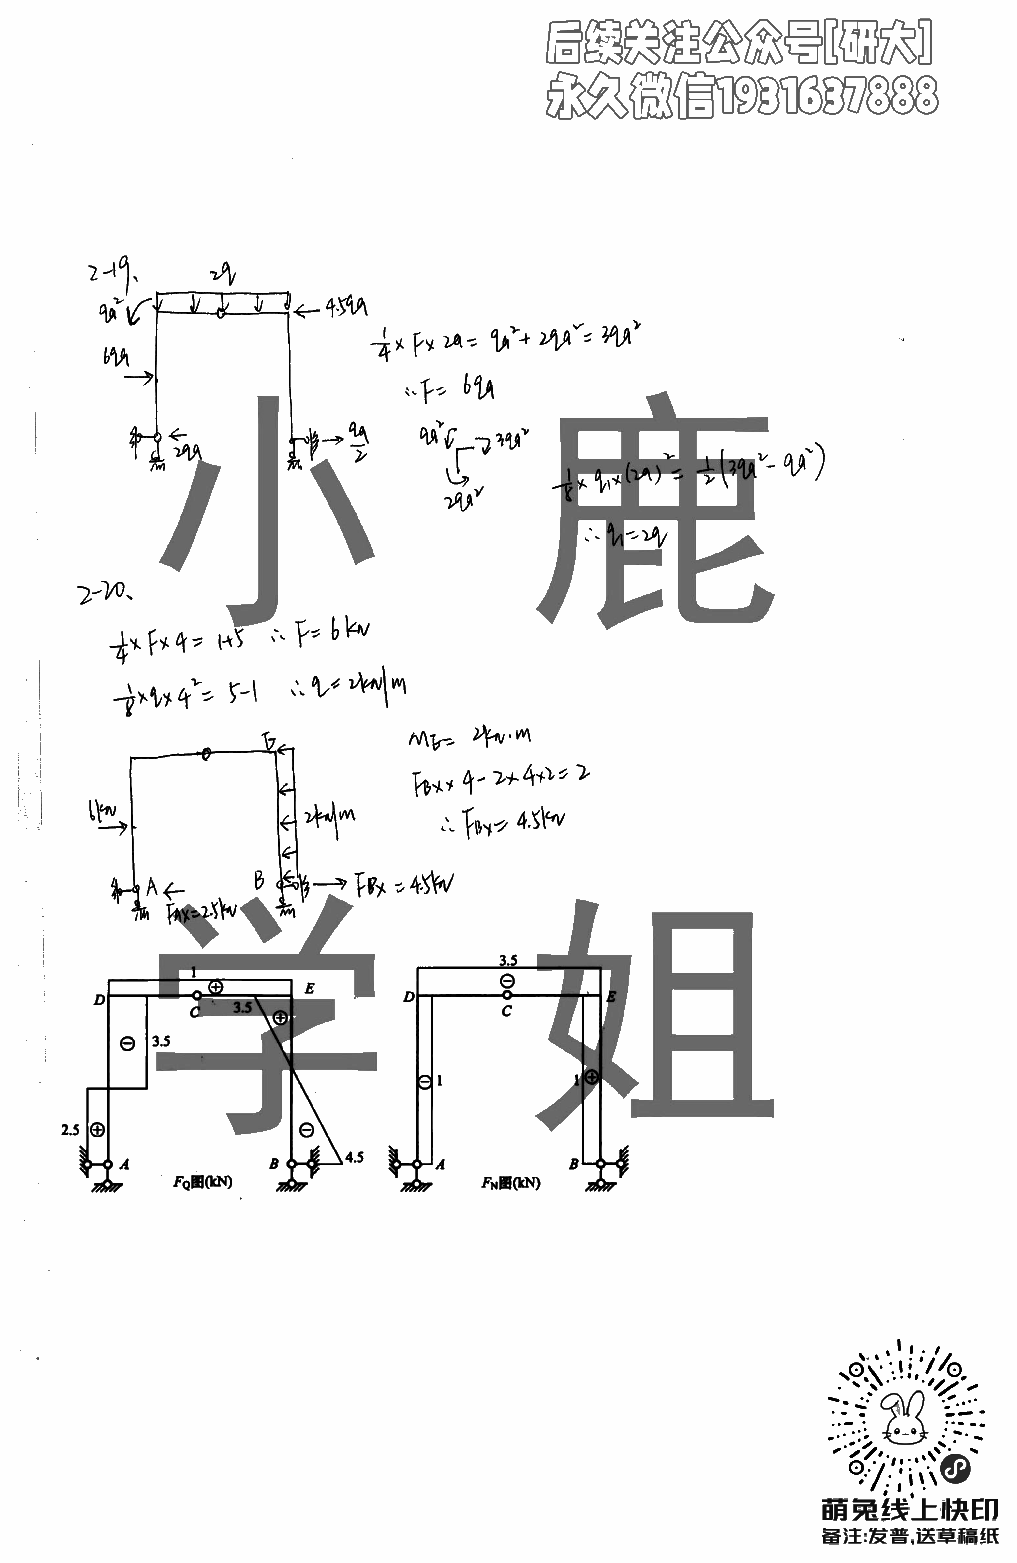
\includegraphics[width=0.96\textwidth,height=0.82\textheight,keepaspectratio]{images/c04_answer_1_p13.png}
\par\small 作业与答案（去水印版），第 13/14 页
\end{center}
\clearpage
\begin{center}
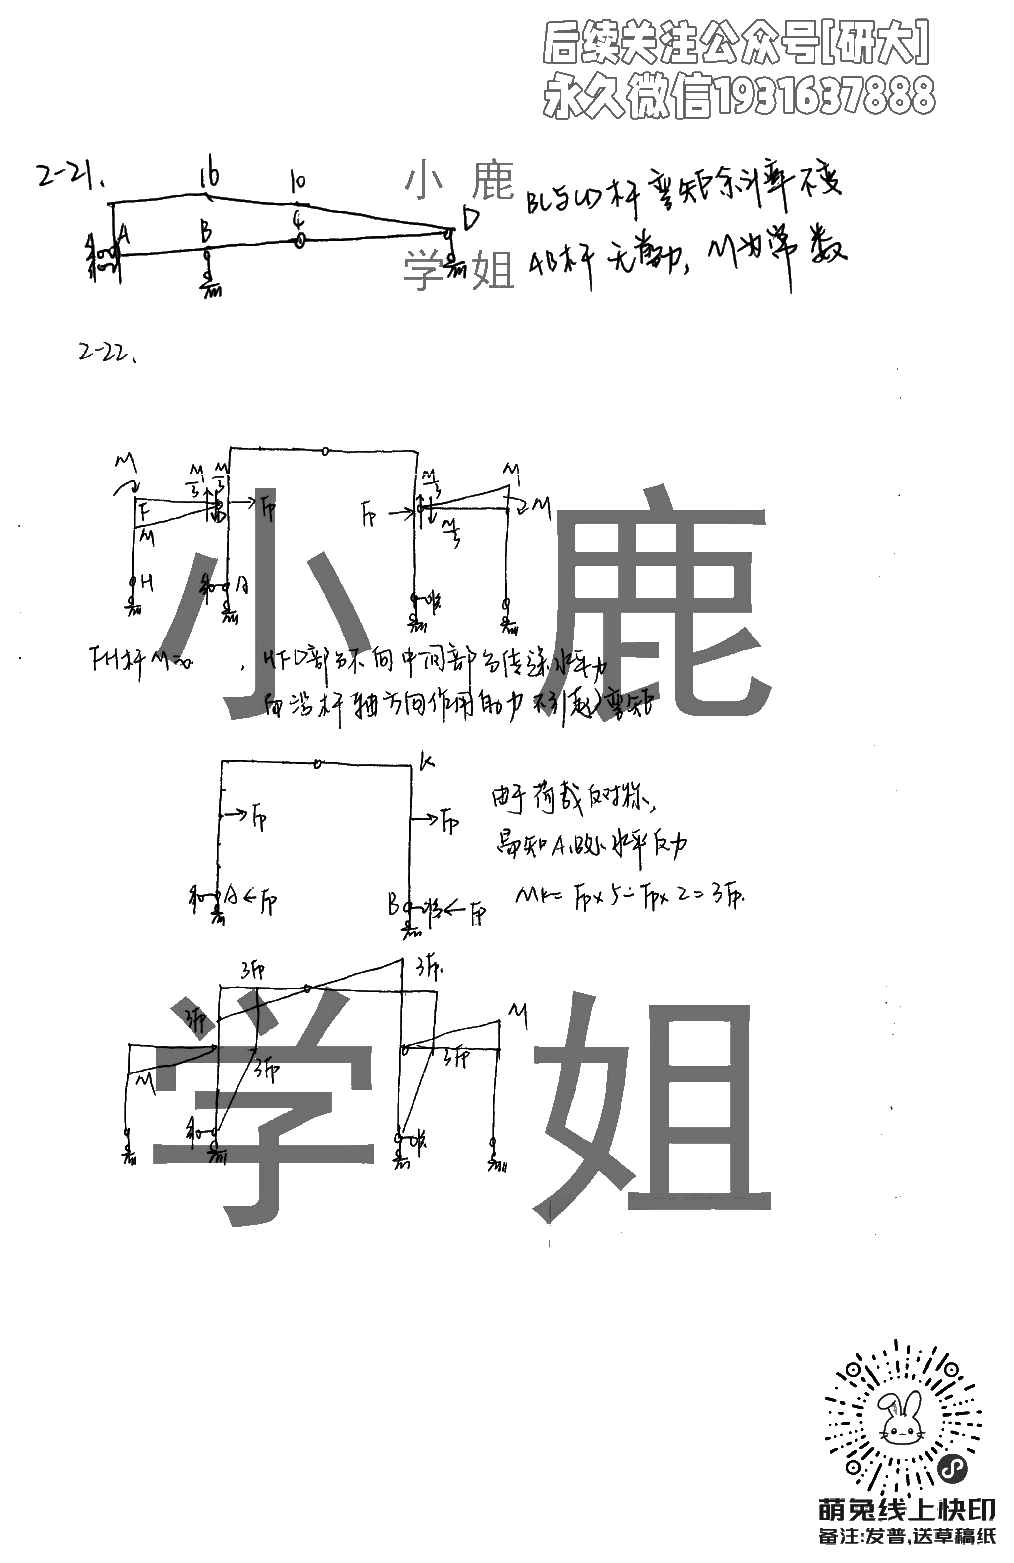
\includegraphics[width=0.96\textwidth,height=0.82\textheight,keepaspectratio]{images/c04_answer_1_p14.png}
\par\small 作业与答案（去水印版），第 14/14 页
\end{center}
\clearpage
\section{讲解笔记（去水印版）}
\begin{center}
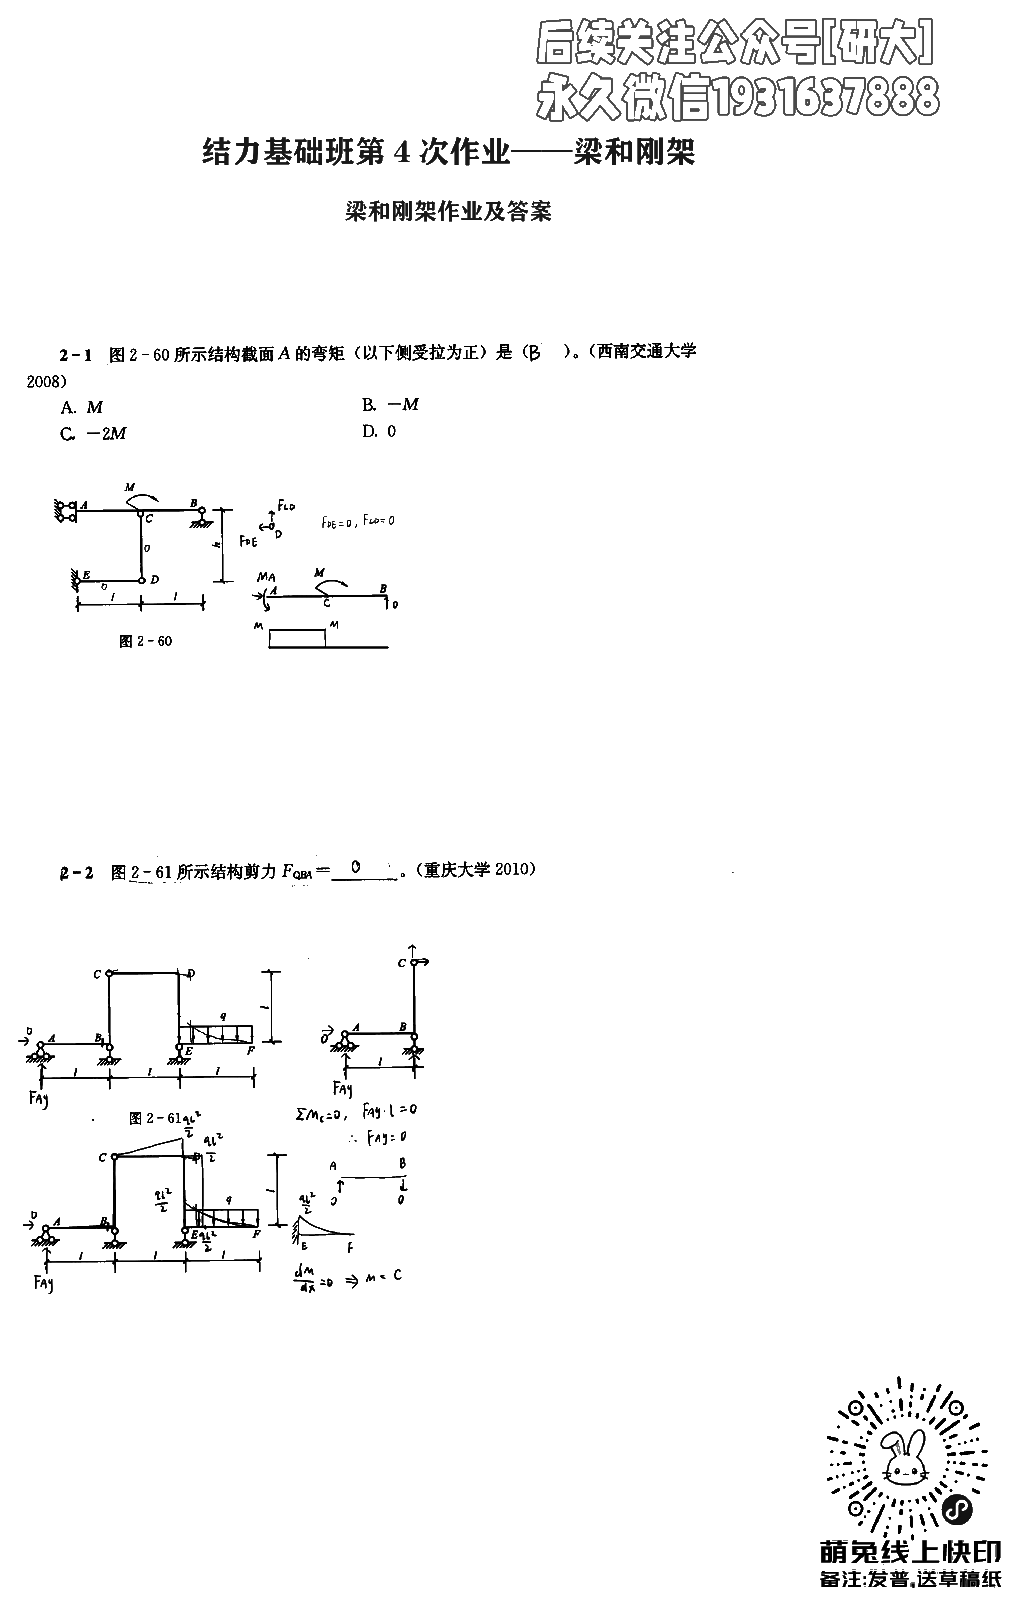
\includegraphics[width=0.96\textwidth,height=0.82\textheight,keepaspectratio]{images/c04_note_p01.png}
\par\small 讲解笔记（去水印版），第 1/11 页
\end{center}
\clearpage
\begin{center}
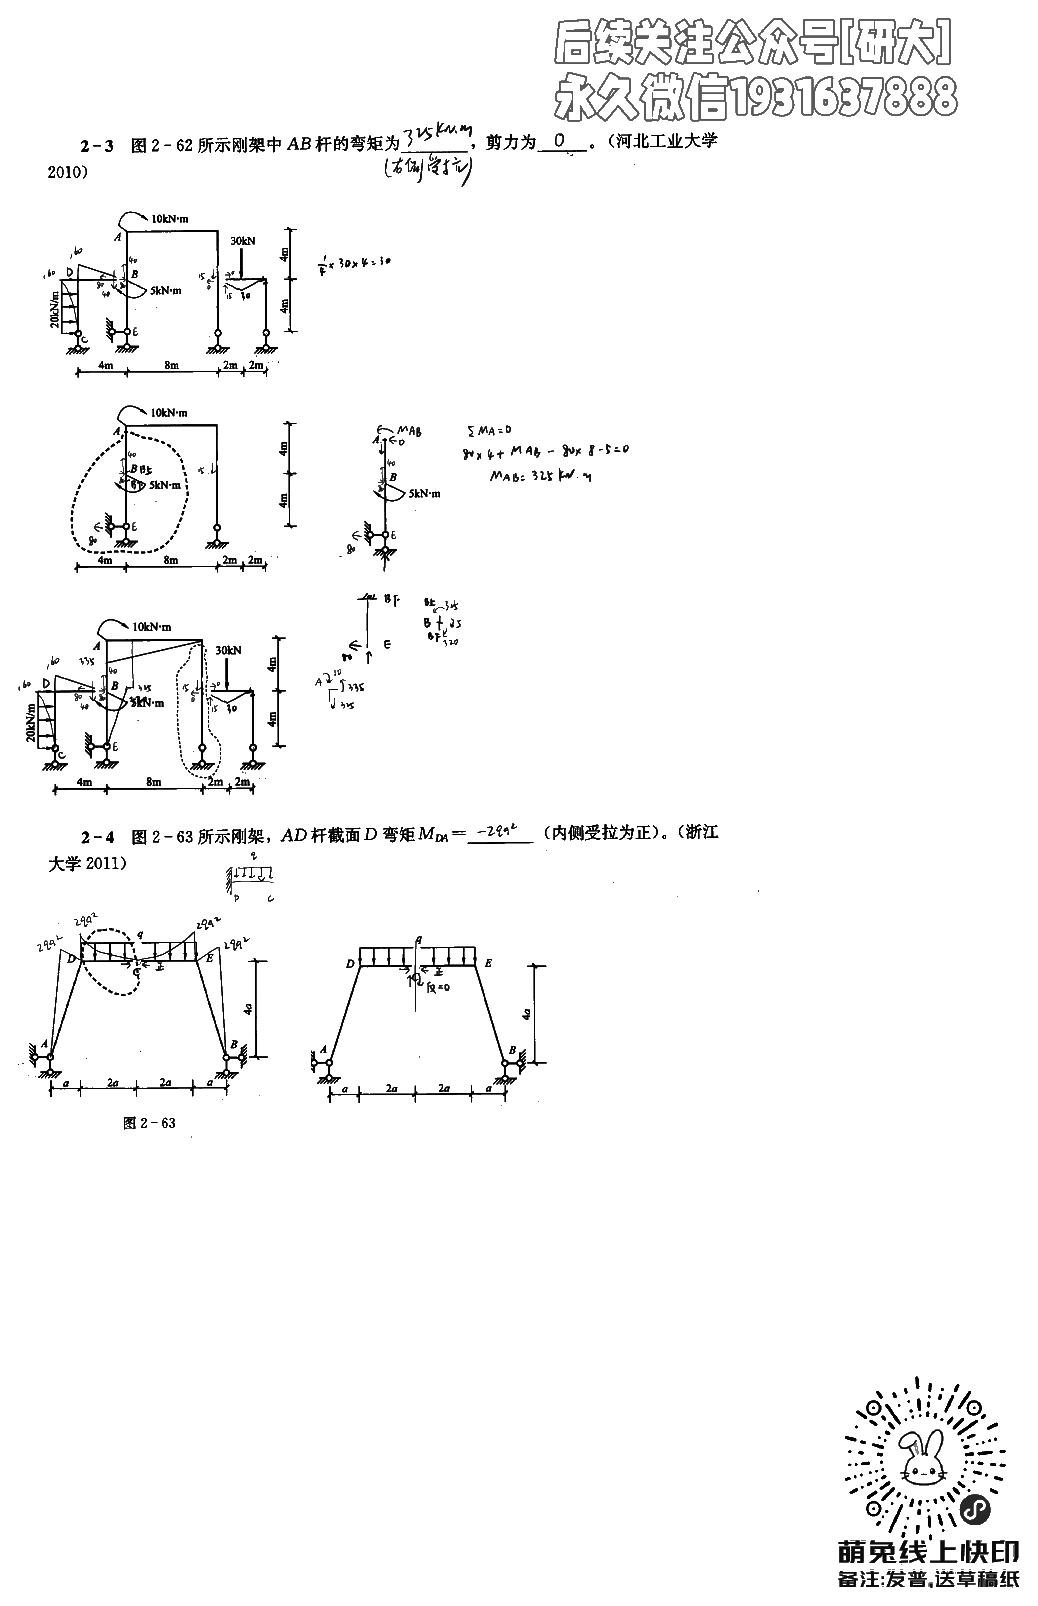
\includegraphics[width=0.96\textwidth,height=0.82\textheight,keepaspectratio]{images/c04_note_p02.png}
\par\small 讲解笔记（去水印版），第 2/11 页
\end{center}
\clearpage
\begin{center}
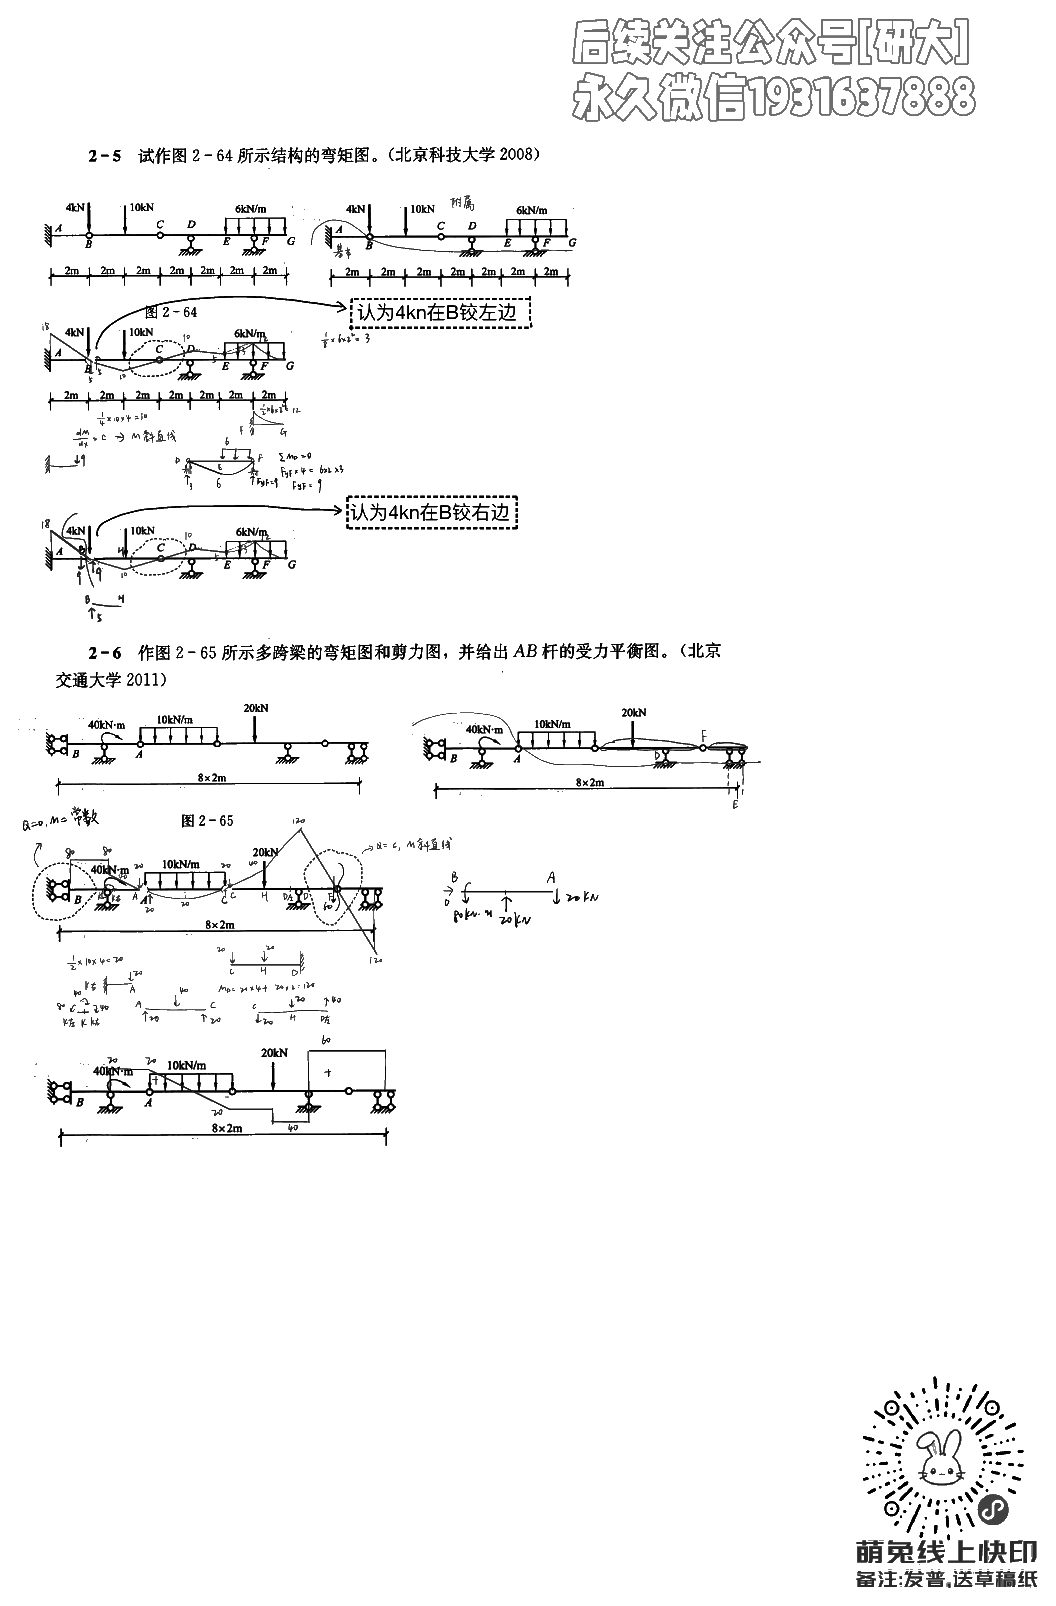
\includegraphics[width=0.96\textwidth,height=0.82\textheight,keepaspectratio]{images/c04_note_p03.png}
\par\small 讲解笔记（去水印版），第 3/11 页
\end{center}
\clearpage
\begin{center}
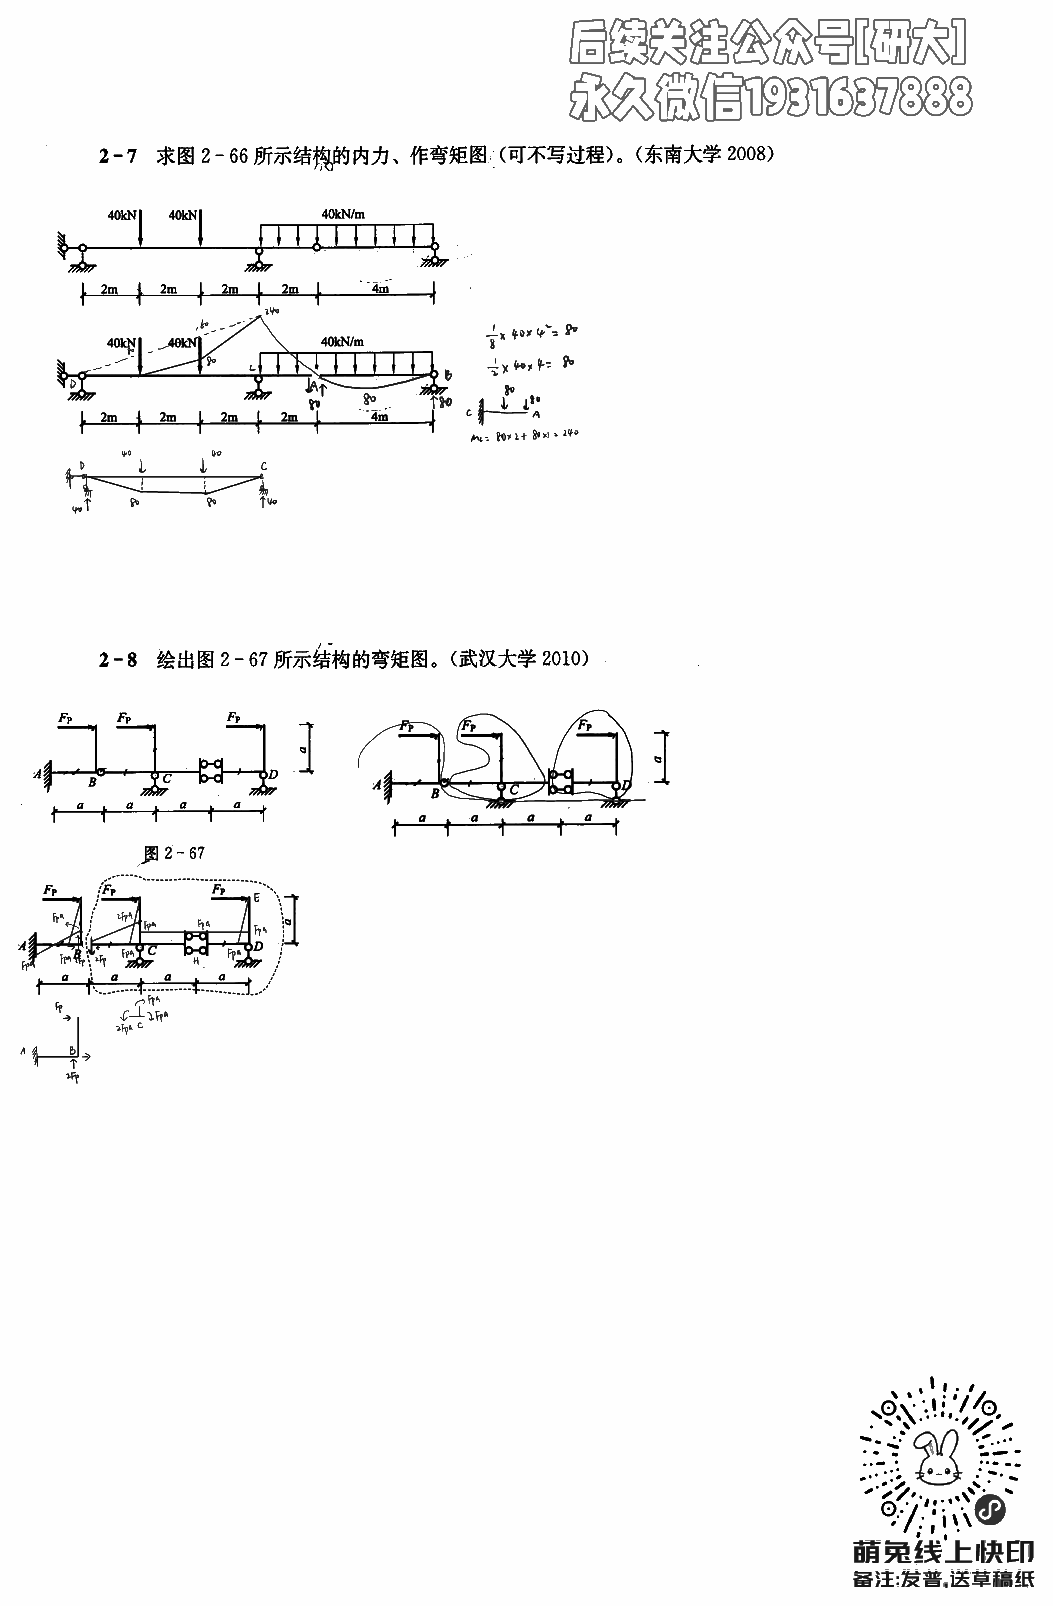
\includegraphics[width=0.96\textwidth,height=0.82\textheight,keepaspectratio]{images/c04_note_p04.png}
\par\small 讲解笔记（去水印版），第 4/11 页
\end{center}
\clearpage
\begin{center}
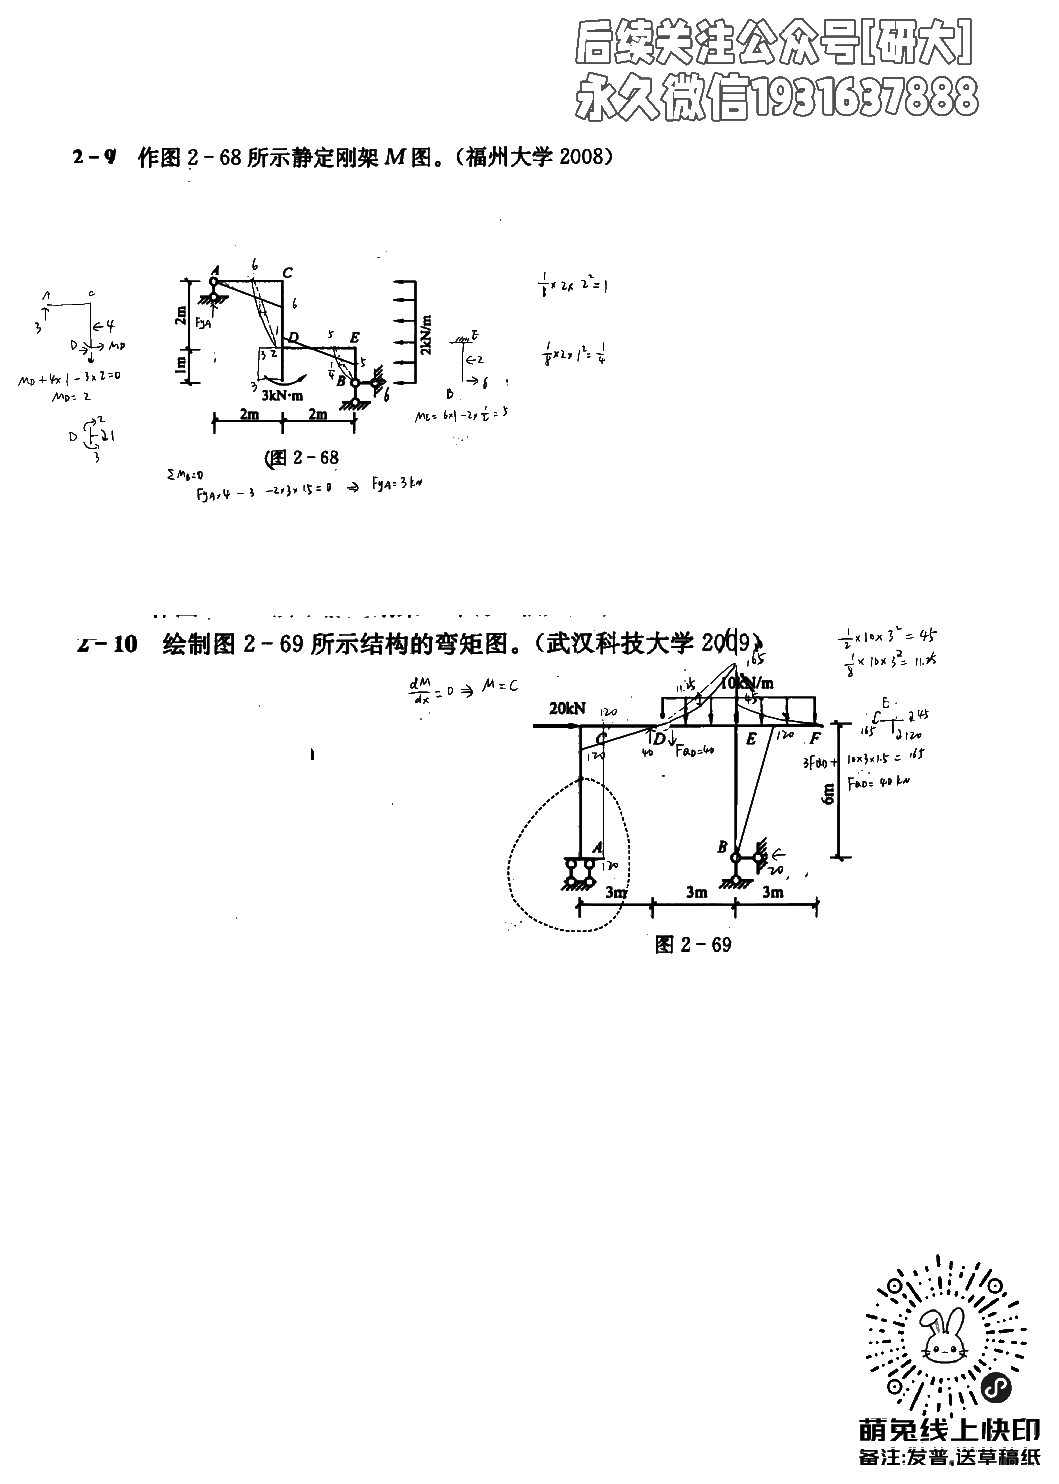
\includegraphics[width=0.96\textwidth,height=0.82\textheight,keepaspectratio]{images/c04_note_p05.png}
\par\small 讲解笔记（去水印版），第 5/11 页
\end{center}
\clearpage
\begin{center}
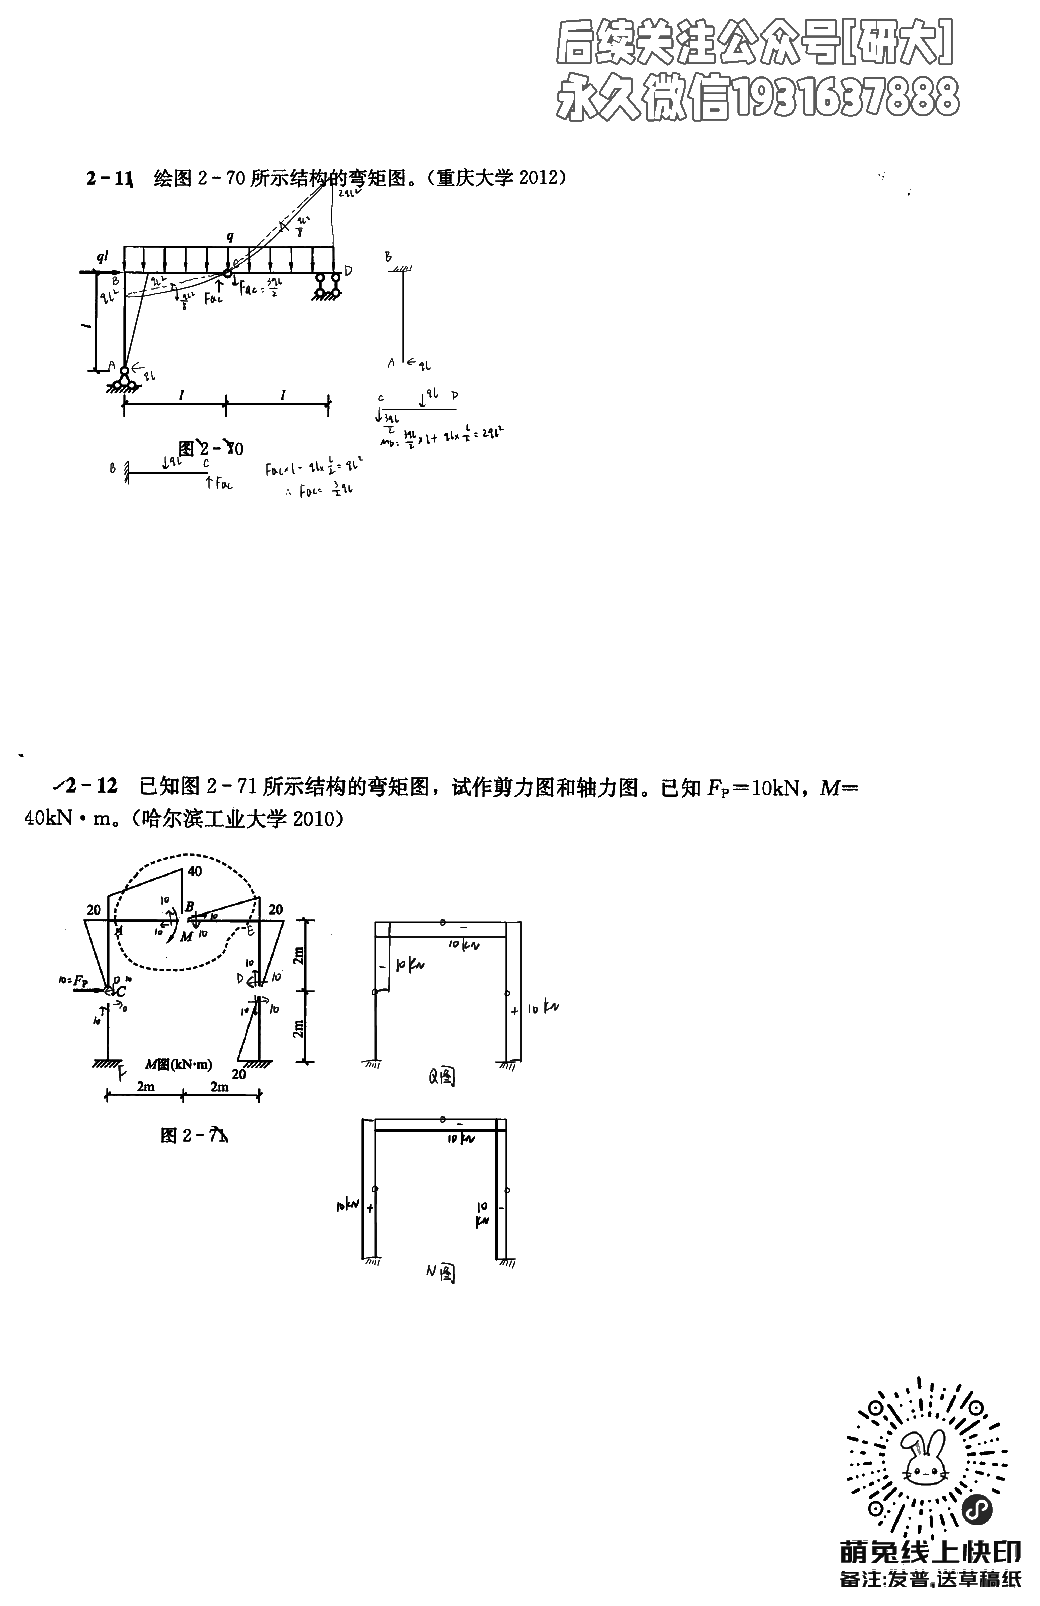
\includegraphics[width=0.96\textwidth,height=0.82\textheight,keepaspectratio]{images/c04_note_p06.png}
\par\small 讲解笔记（去水印版），第 6/11 页
\end{center}
\clearpage
\begin{center}
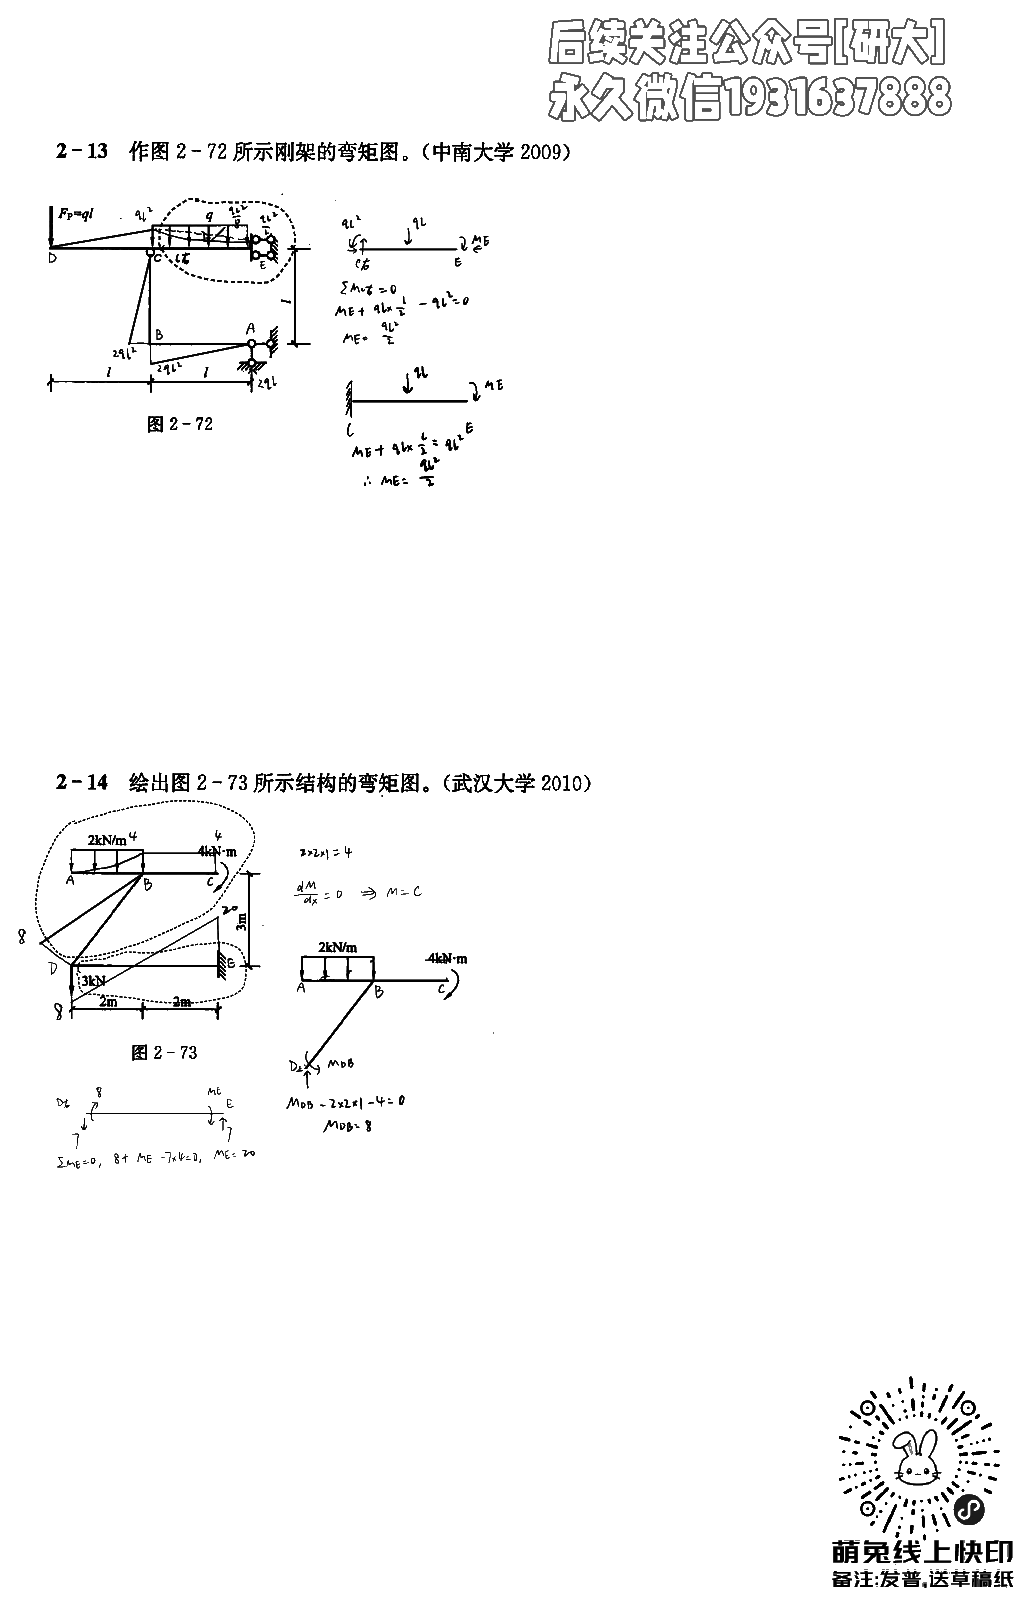
\includegraphics[width=0.96\textwidth,height=0.82\textheight,keepaspectratio]{images/c04_note_p07.png}
\par\small 讲解笔记（去水印版），第 7/11 页
\end{center}
\clearpage
\begin{center}
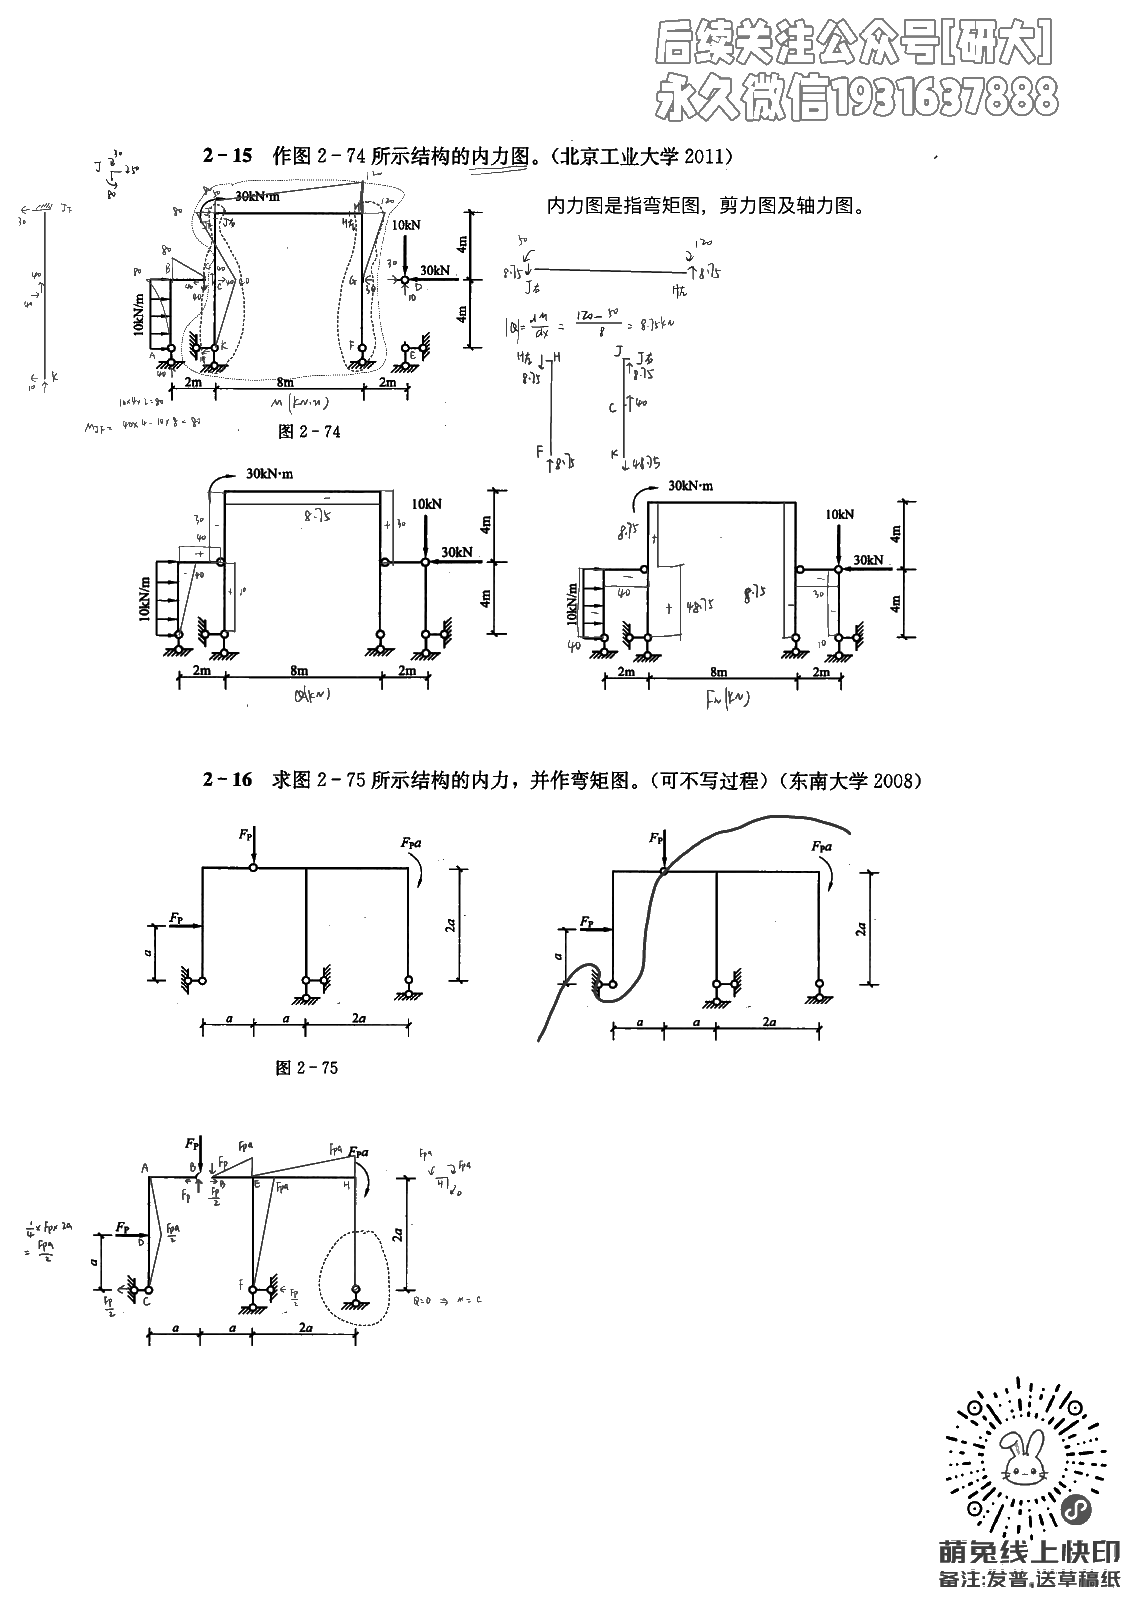
\includegraphics[width=0.96\textwidth,height=0.82\textheight,keepaspectratio]{images/c04_note_p08.png}
\par\small 讲解笔记（去水印版），第 8/11 页
\end{center}
\clearpage
\begin{center}
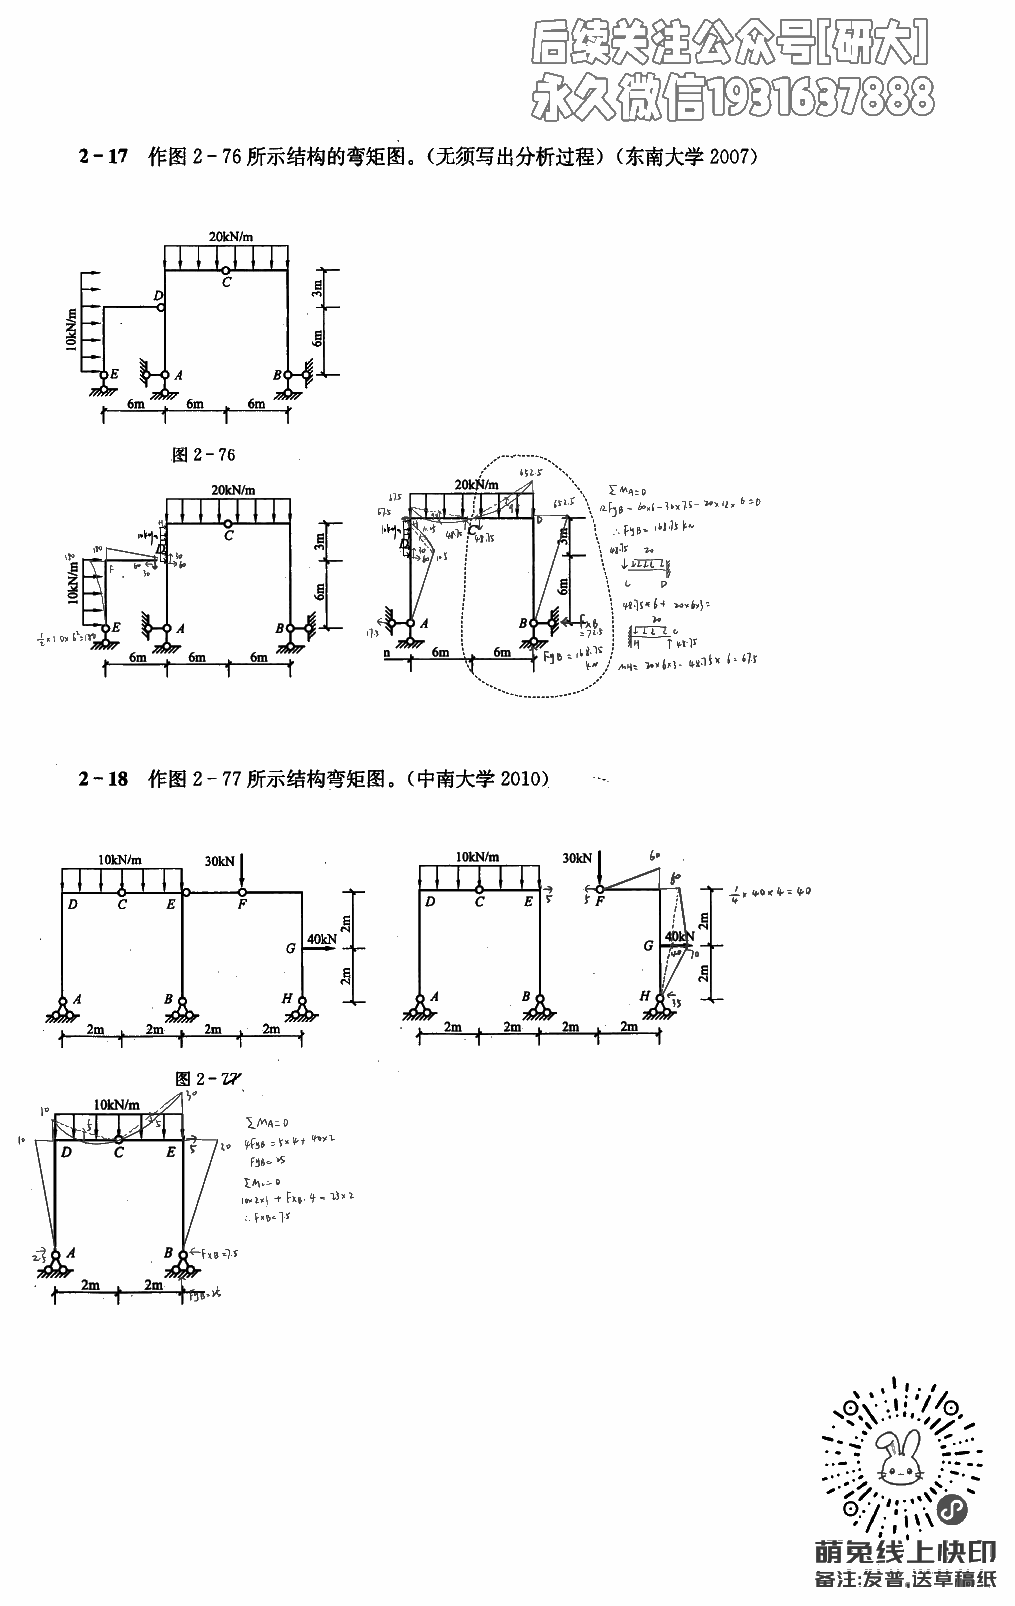
\includegraphics[width=0.96\textwidth,height=0.82\textheight,keepaspectratio]{images/c04_note_p09.png}
\par\small 讲解笔记（去水印版），第 9/11 页
\end{center}
\clearpage
\begin{center}
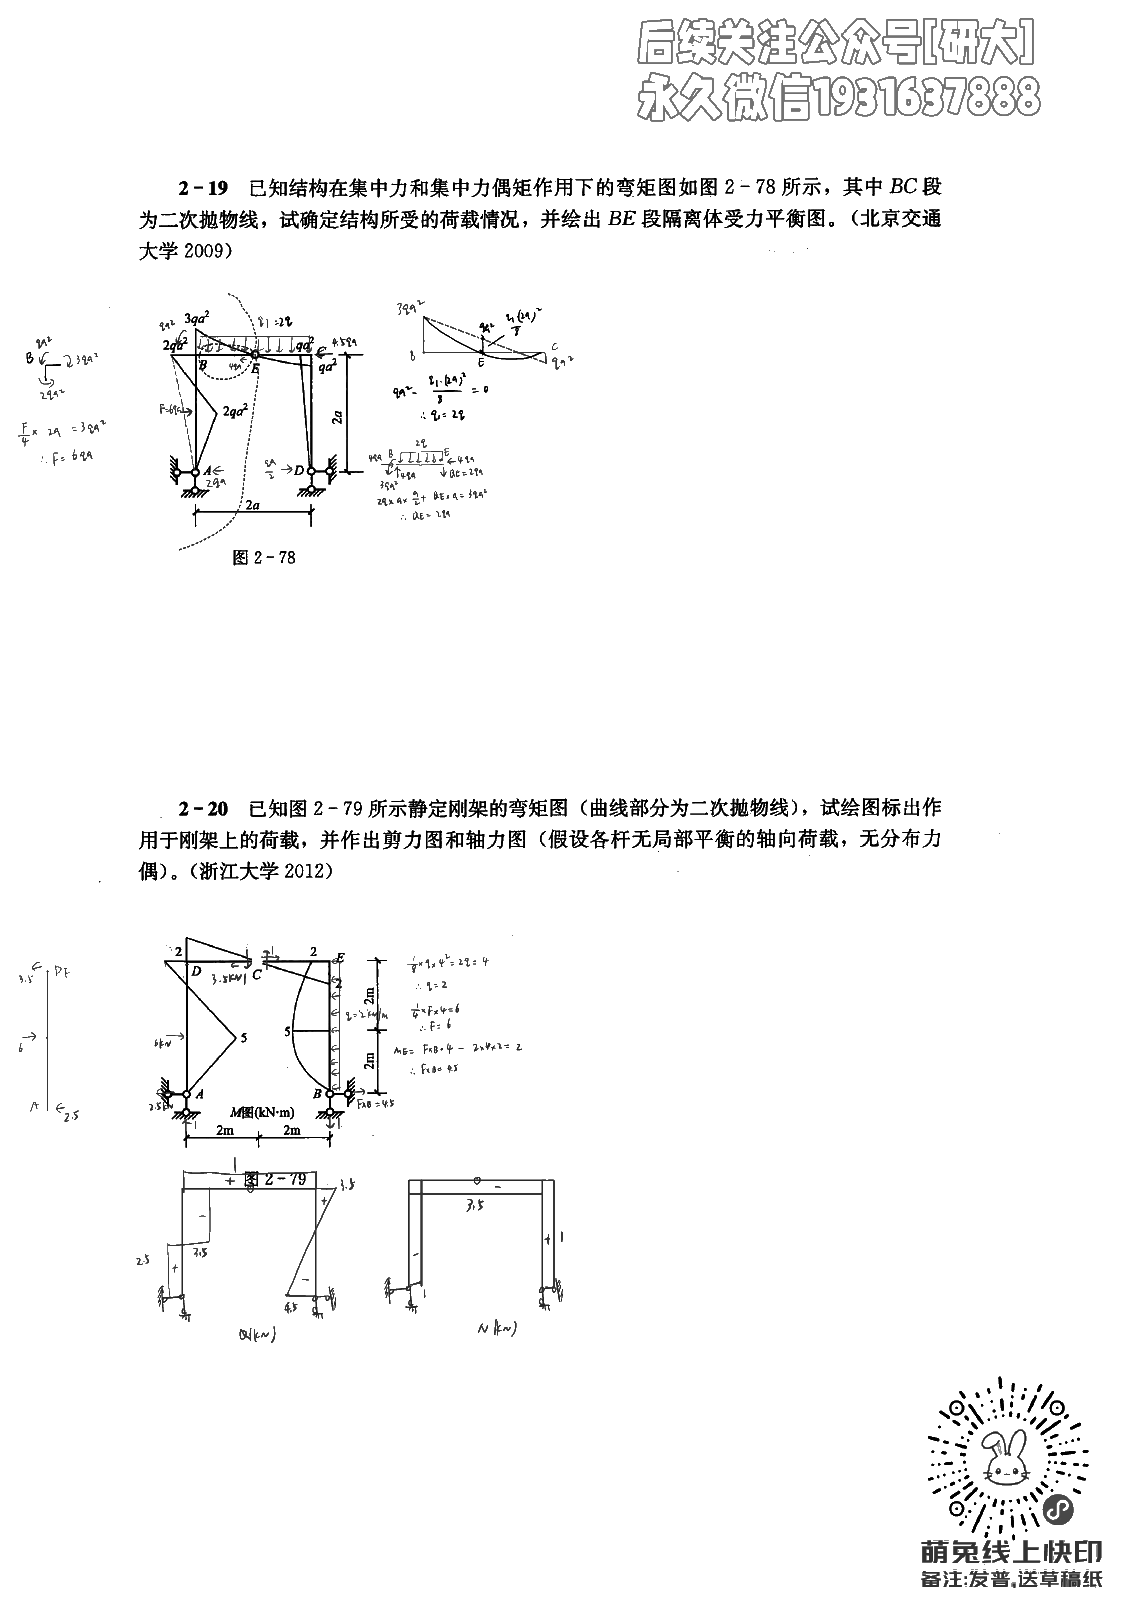
\includegraphics[width=0.96\textwidth,height=0.82\textheight,keepaspectratio]{images/c04_note_p10.png}
\par\small 讲解笔记（去水印版），第 10/11 页
\end{center}
\clearpage
\begin{center}
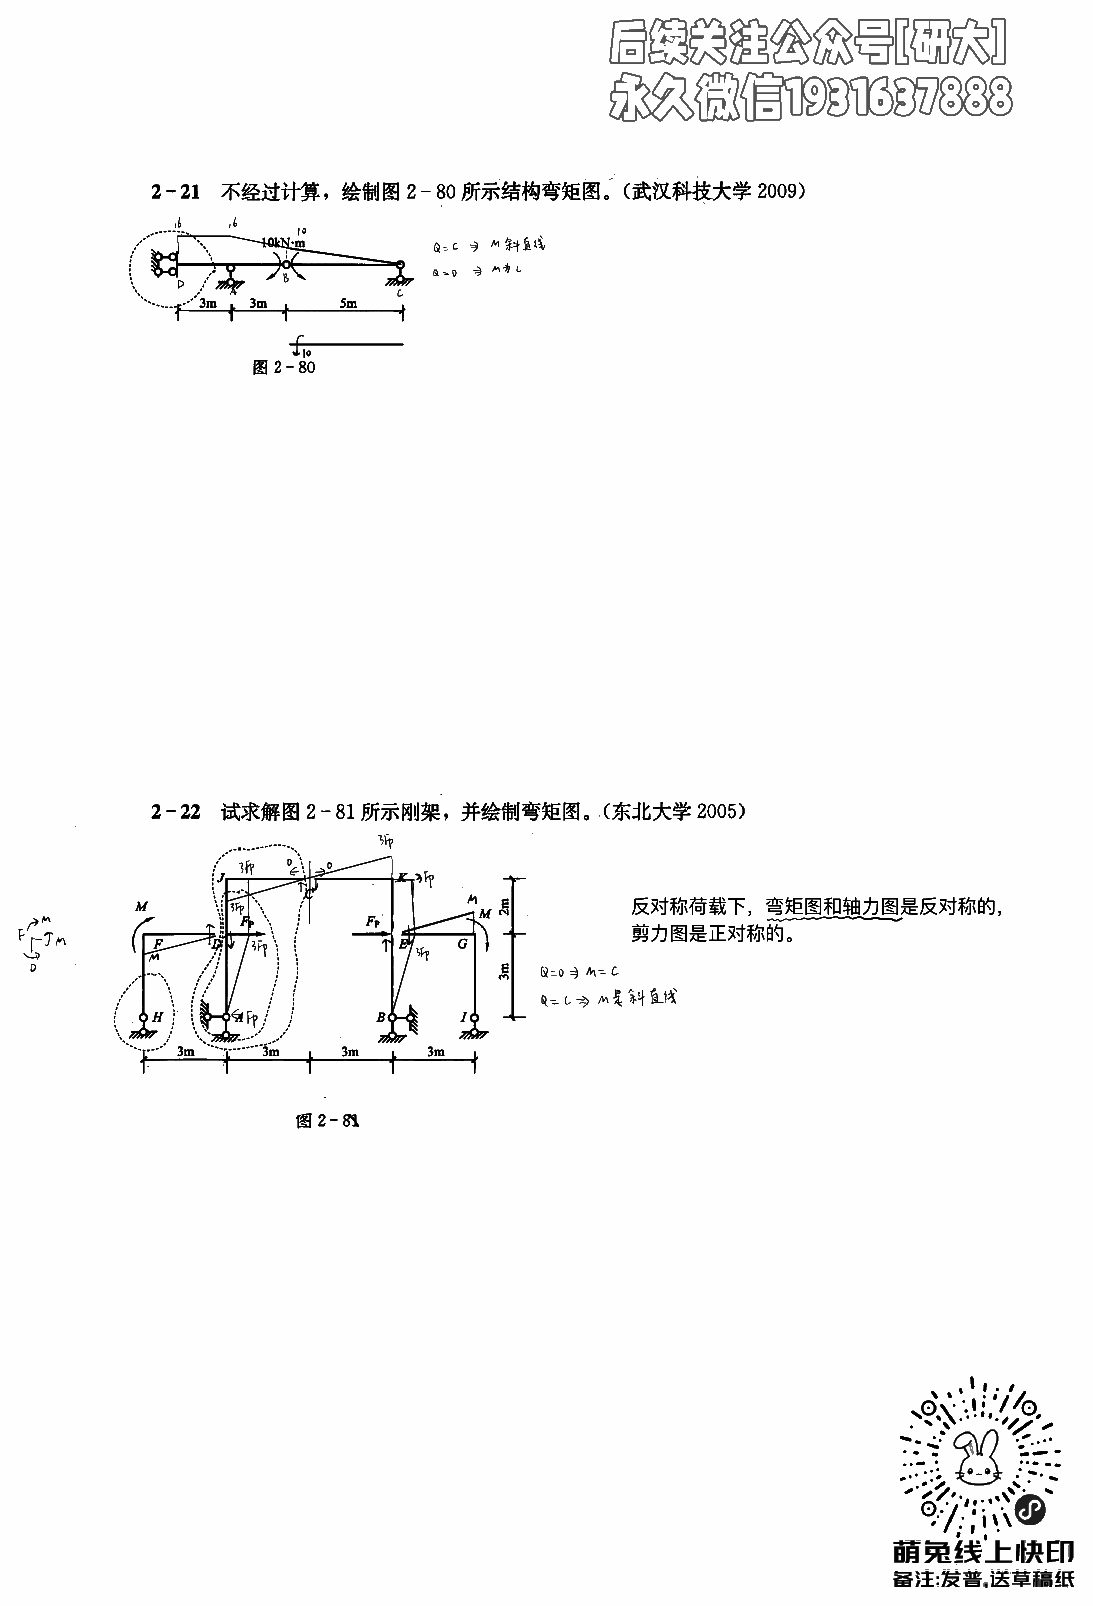
\includegraphics[width=0.96\textwidth,height=0.82\textheight,keepaspectratio]{images/c04_note_p11.png}
\par\small 讲解笔记（去水印版），第 11/11 页
\end{center}
\clearpage
\chapter{第5讲：静定桁架}
\begin{tcolorbox}[title=解析要点]
静定桁架优先识别零杆，再结合节点法和截面法。节点法适合逐点推进，截面法适合直接求少数目标杆力。
\end{tcolorbox}
\begin{tcolorbox}[title=答案与校核]
答案页给出桁架杆力计算；正负号分别对应受拉、受压，零杆应单独标明。
\end{tcolorbox}
\section{作业与答案（去水印版）}
\begin{center}
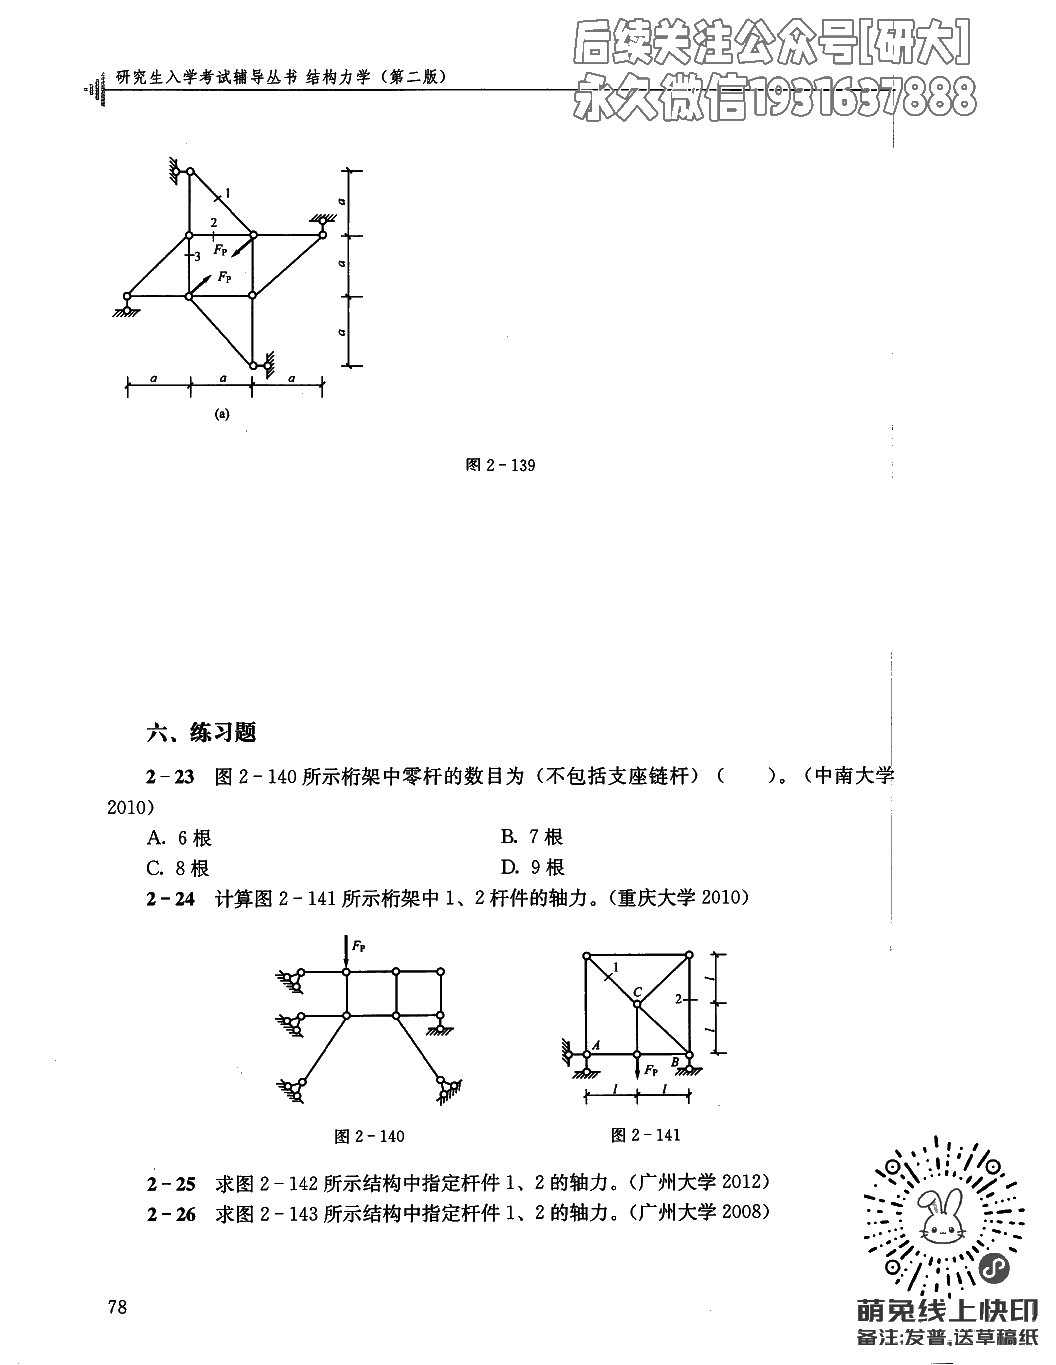
\includegraphics[width=0.96\textwidth,height=0.82\textheight,keepaspectratio]{images/c05_answer_1_p01.png}
\par\small 作业与答案（去水印版），第 1/3 页
\end{center}
\clearpage
\begin{center}
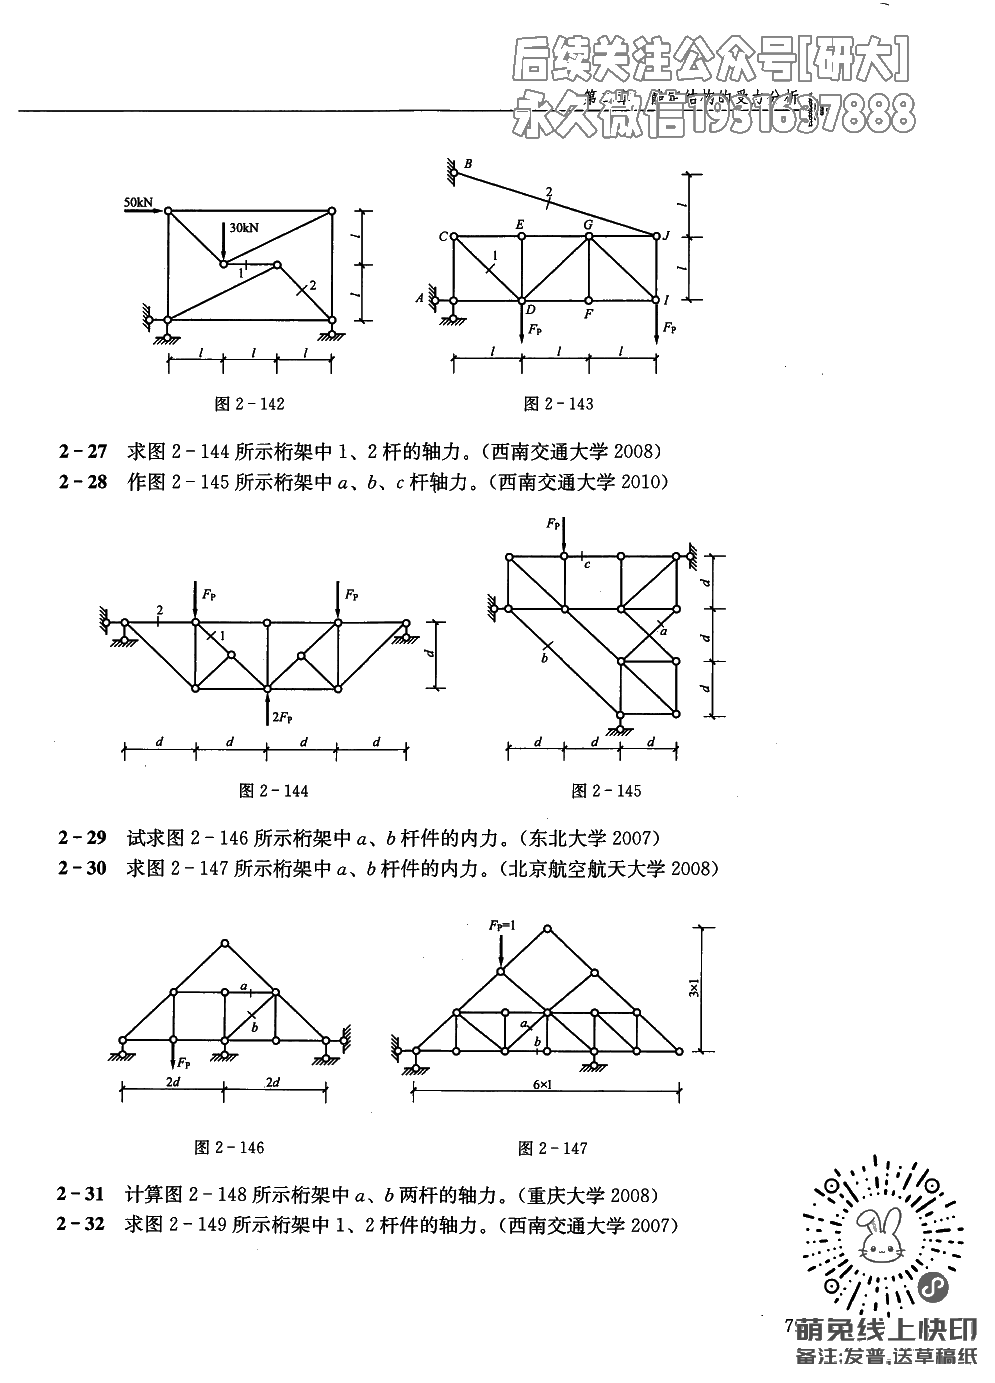
\includegraphics[width=0.96\textwidth,height=0.82\textheight,keepaspectratio]{images/c05_answer_1_p02.png}
\par\small 作业与答案（去水印版），第 2/3 页
\end{center}
\clearpage
\begin{center}
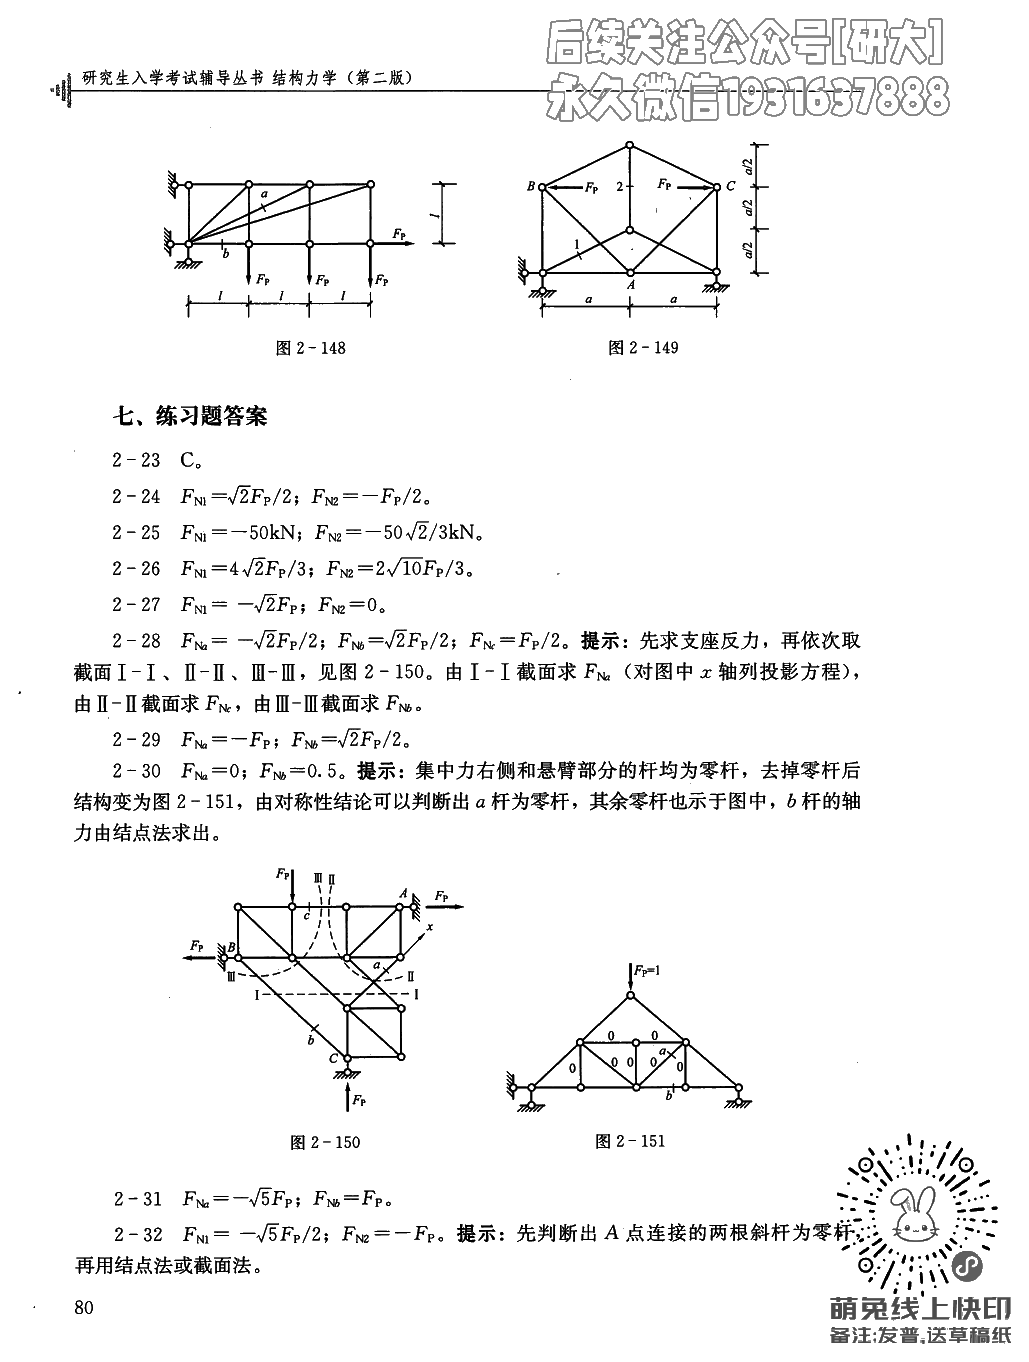
\includegraphics[width=0.96\textwidth,height=0.82\textheight,keepaspectratio]{images/c05_answer_1_p03.png}
\par\small 作业与答案（去水印版），第 3/3 页
\end{center}
\clearpage
\section{讲解笔记（去水印版）}
\begin{center}
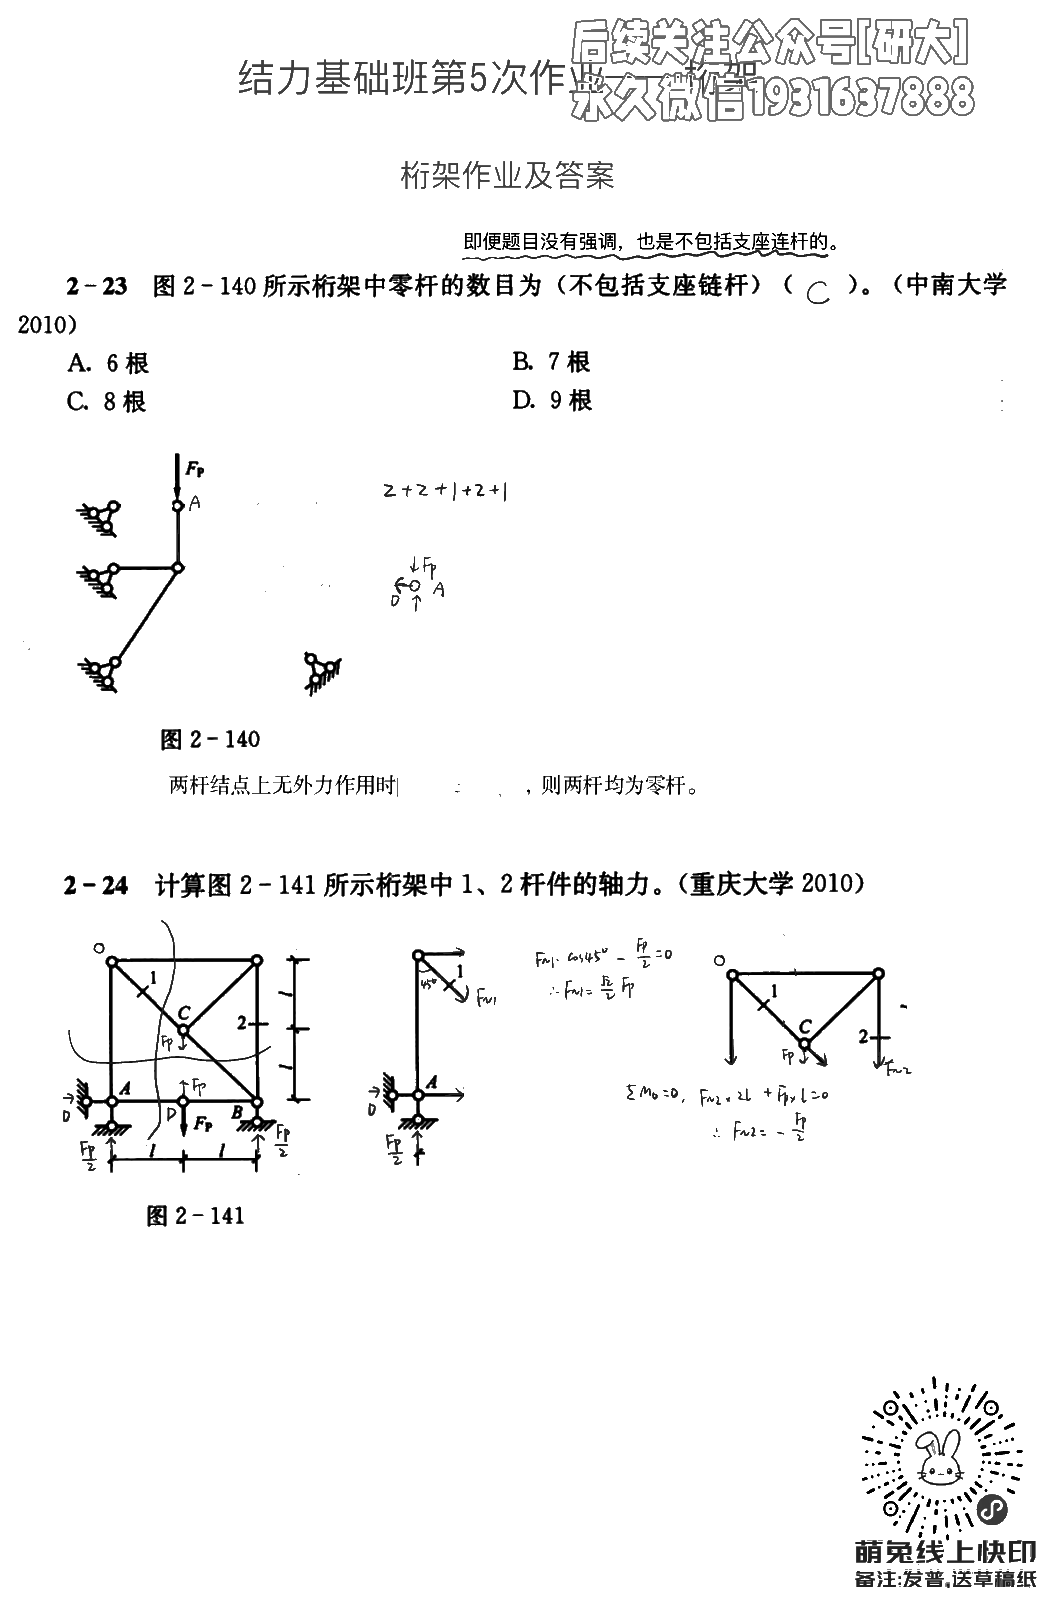
\includegraphics[width=0.96\textwidth,height=0.82\textheight,keepaspectratio]{images/c05_note_p01.png}
\par\small 讲解笔记（去水印版），第 1/5 页
\end{center}
\clearpage
\begin{center}
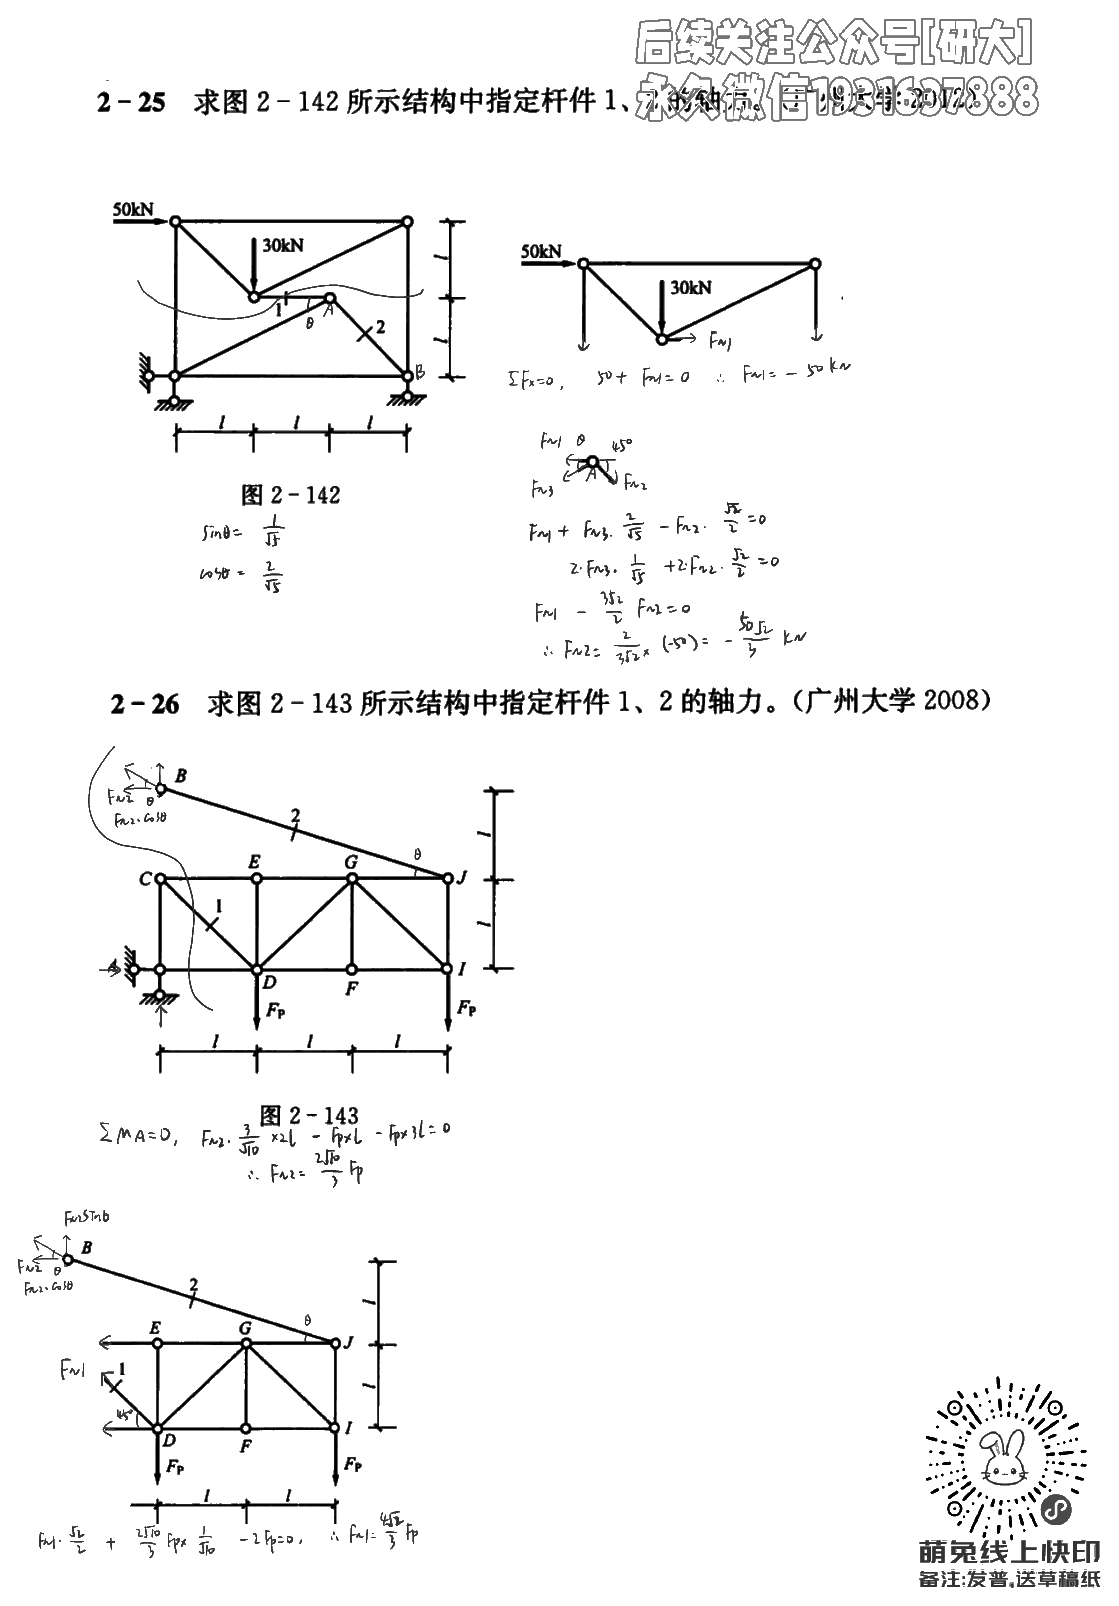
\includegraphics[width=0.96\textwidth,height=0.82\textheight,keepaspectratio]{images/c05_note_p02.png}
\par\small 讲解笔记（去水印版），第 2/5 页
\end{center}
\clearpage
\begin{center}
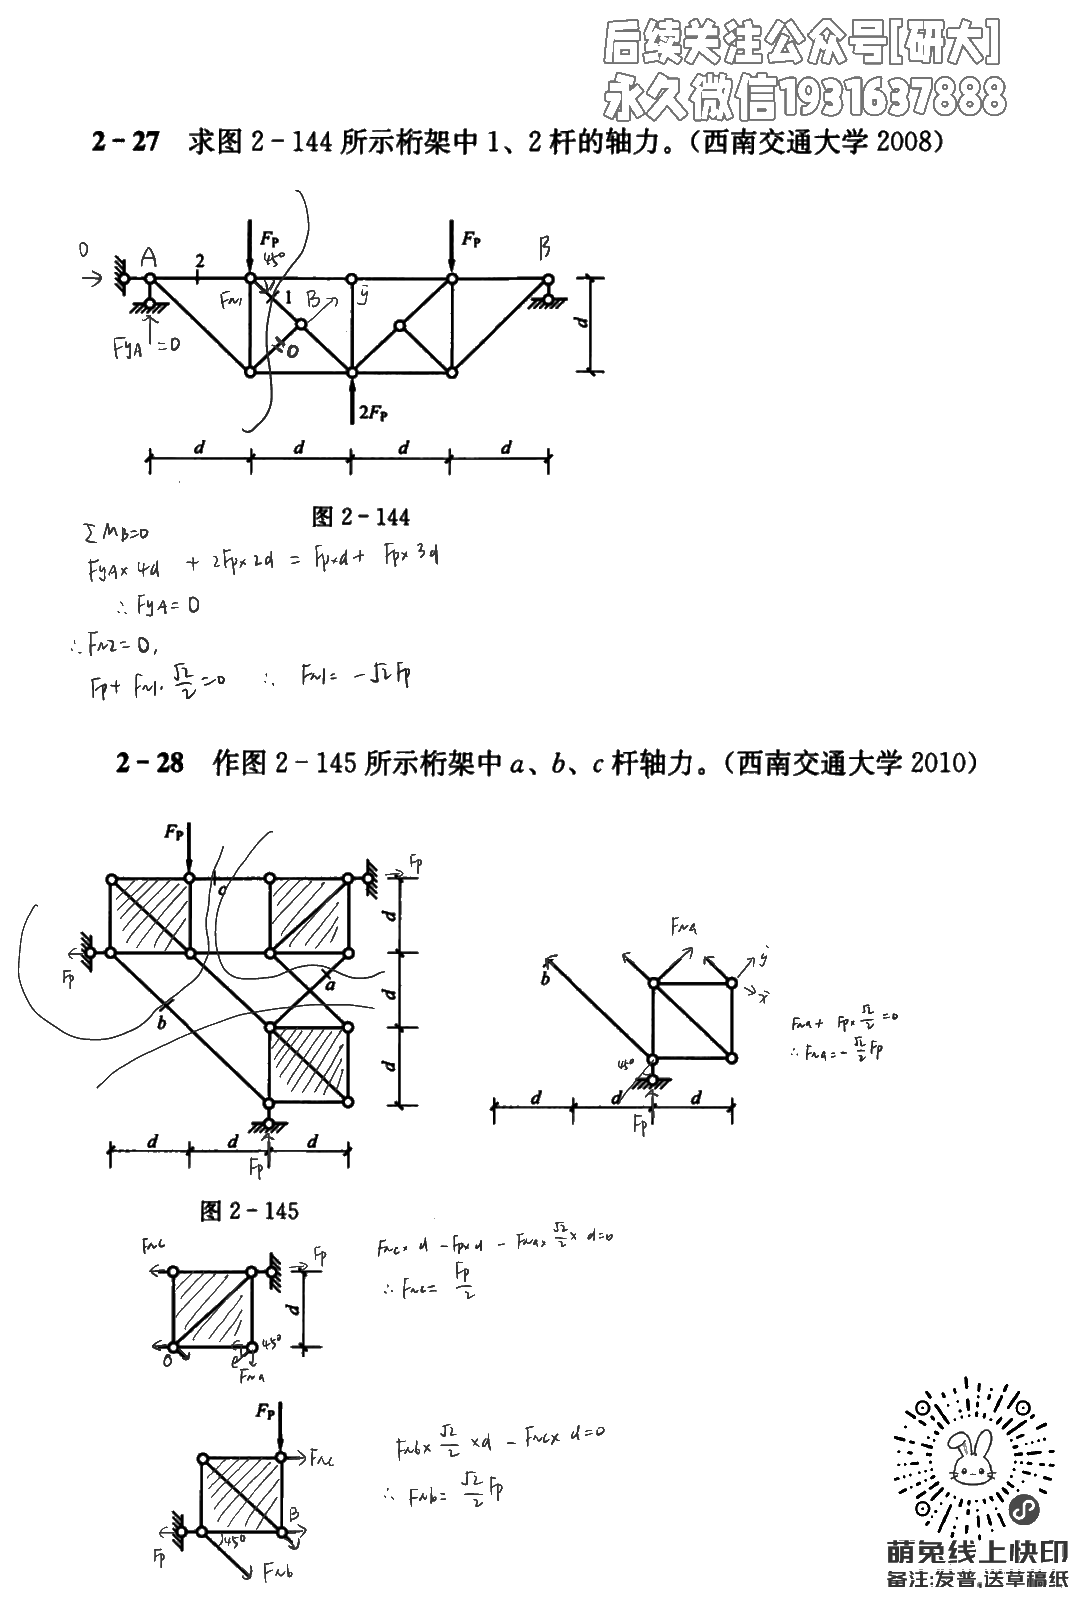
\includegraphics[width=0.96\textwidth,height=0.82\textheight,keepaspectratio]{images/c05_note_p03.png}
\par\small 讲解笔记（去水印版），第 3/5 页
\end{center}
\clearpage
\begin{center}
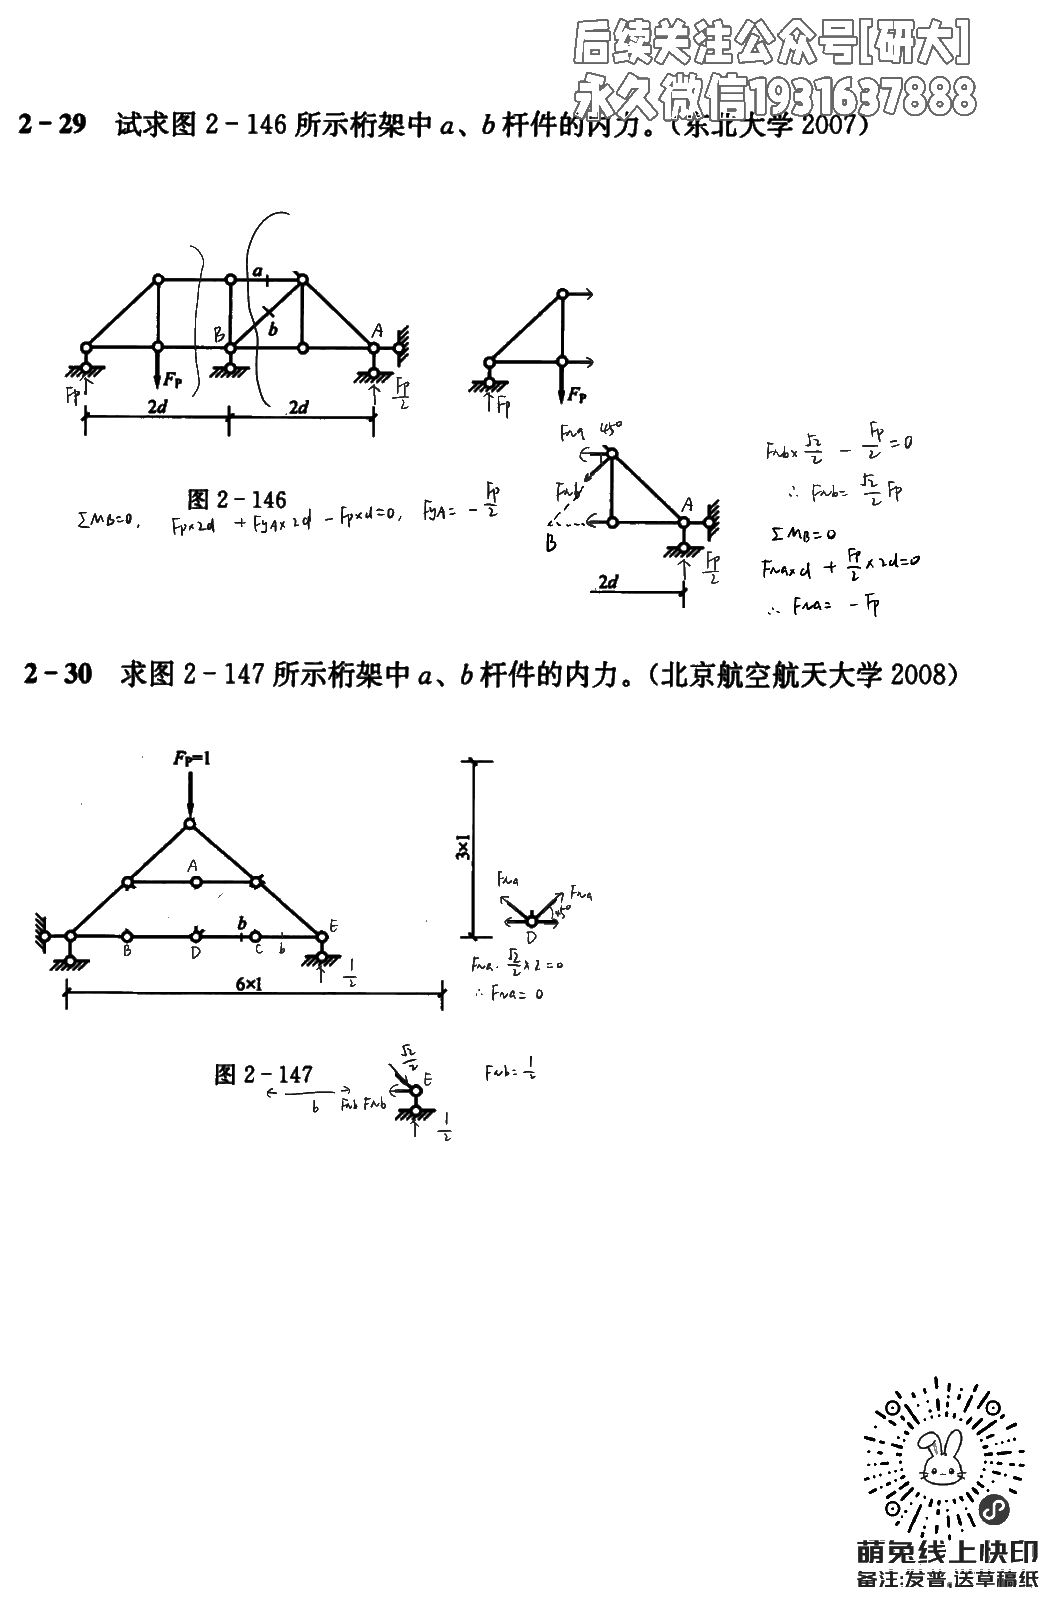
\includegraphics[width=0.96\textwidth,height=0.82\textheight,keepaspectratio]{images/c05_note_p04.png}
\par\small 讲解笔记（去水印版），第 4/5 页
\end{center}
\clearpage
\begin{center}
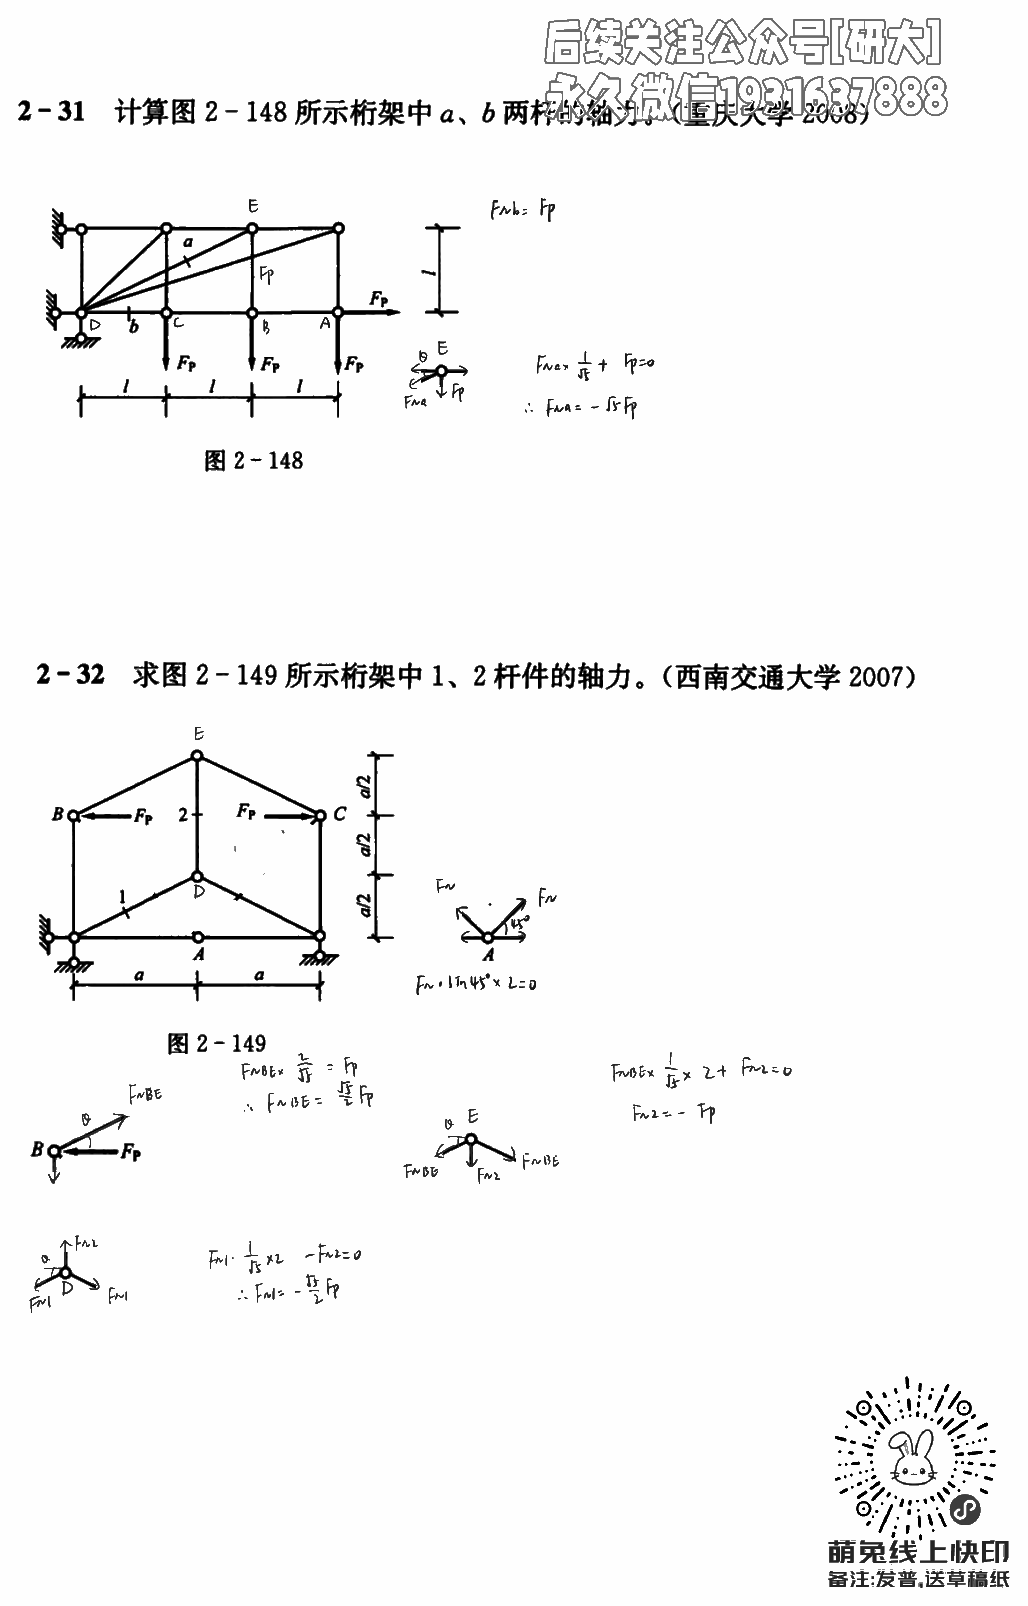
\includegraphics[width=0.96\textwidth,height=0.82\textheight,keepaspectratio]{images/c05_note_p05.png}
\par\small 讲解笔记（去水印版），第 5/5 页
\end{center}
\clearpage
\chapter{第6讲：组合结构}
\begin{tcolorbox}[title=解析要点]
组合结构要先辨认桁架杆、梁式杆和刚架部分的传力特点。解题时按连接点拆分子结构，保证连接处作用力与反作用力成对一致。
\end{tcolorbox}
\begin{tcolorbox}[title=答案与校核]
答案页给出组合结构拆分和受力计算；连接处内力平衡是主要校核点。
\end{tcolorbox}
\section{作业与答案（去水印版）}
\begin{center}
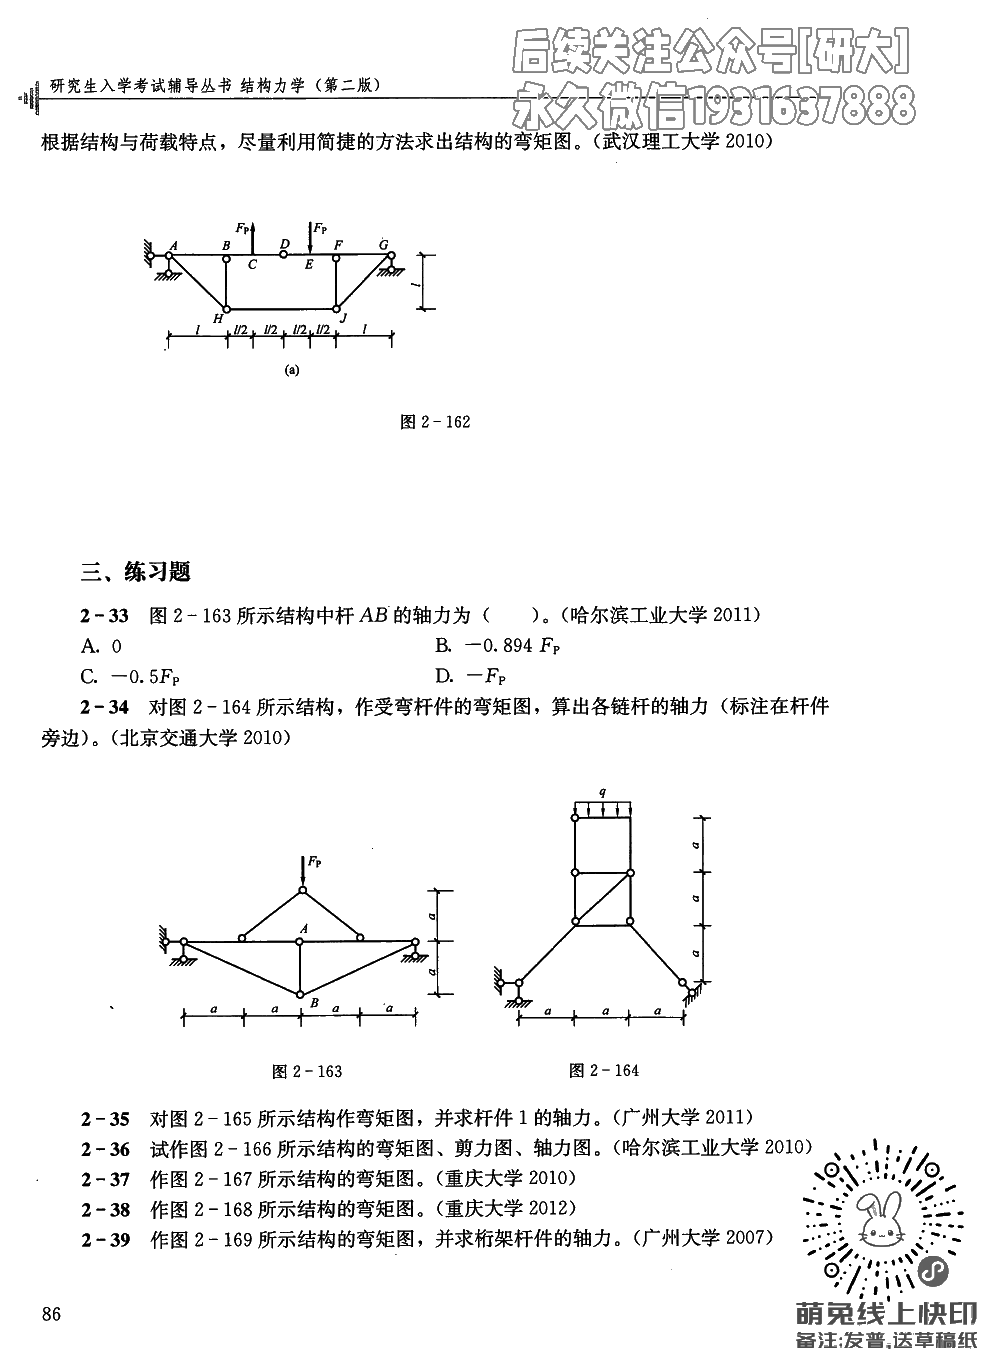
\includegraphics[width=0.96\textwidth,height=0.82\textheight,keepaspectratio]{images/c06_answer_1_p01.png}
\par\small 作业与答案（去水印版），第 1/3 页
\end{center}
\clearpage
\begin{center}
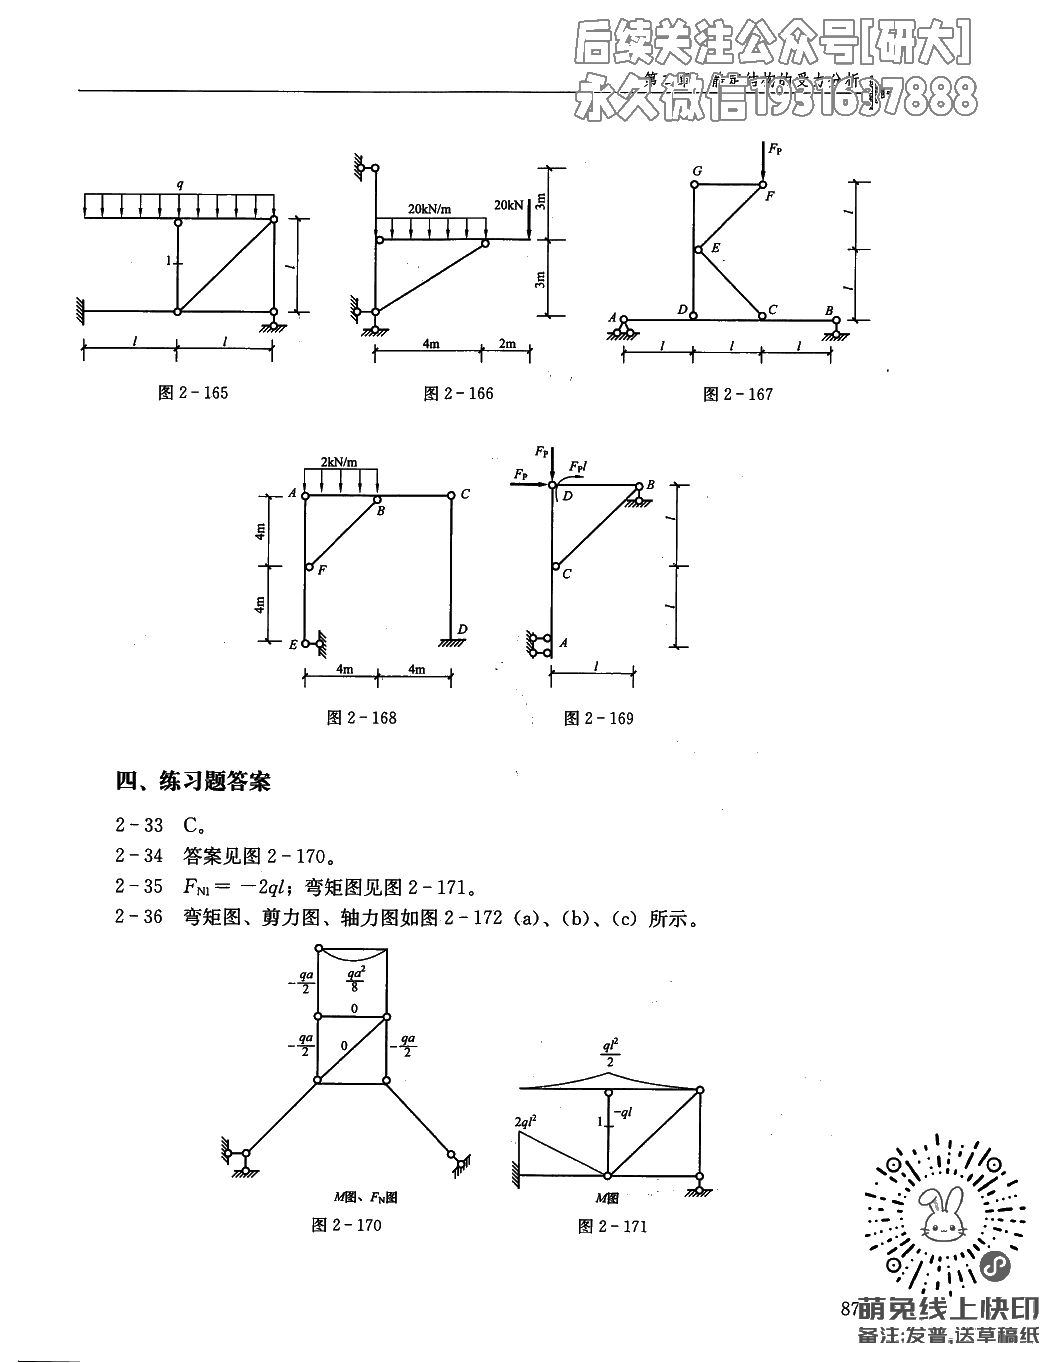
\includegraphics[width=0.96\textwidth,height=0.82\textheight,keepaspectratio]{images/c06_answer_1_p02.png}
\par\small 作业与答案（去水印版），第 2/3 页
\end{center}
\clearpage
\begin{center}
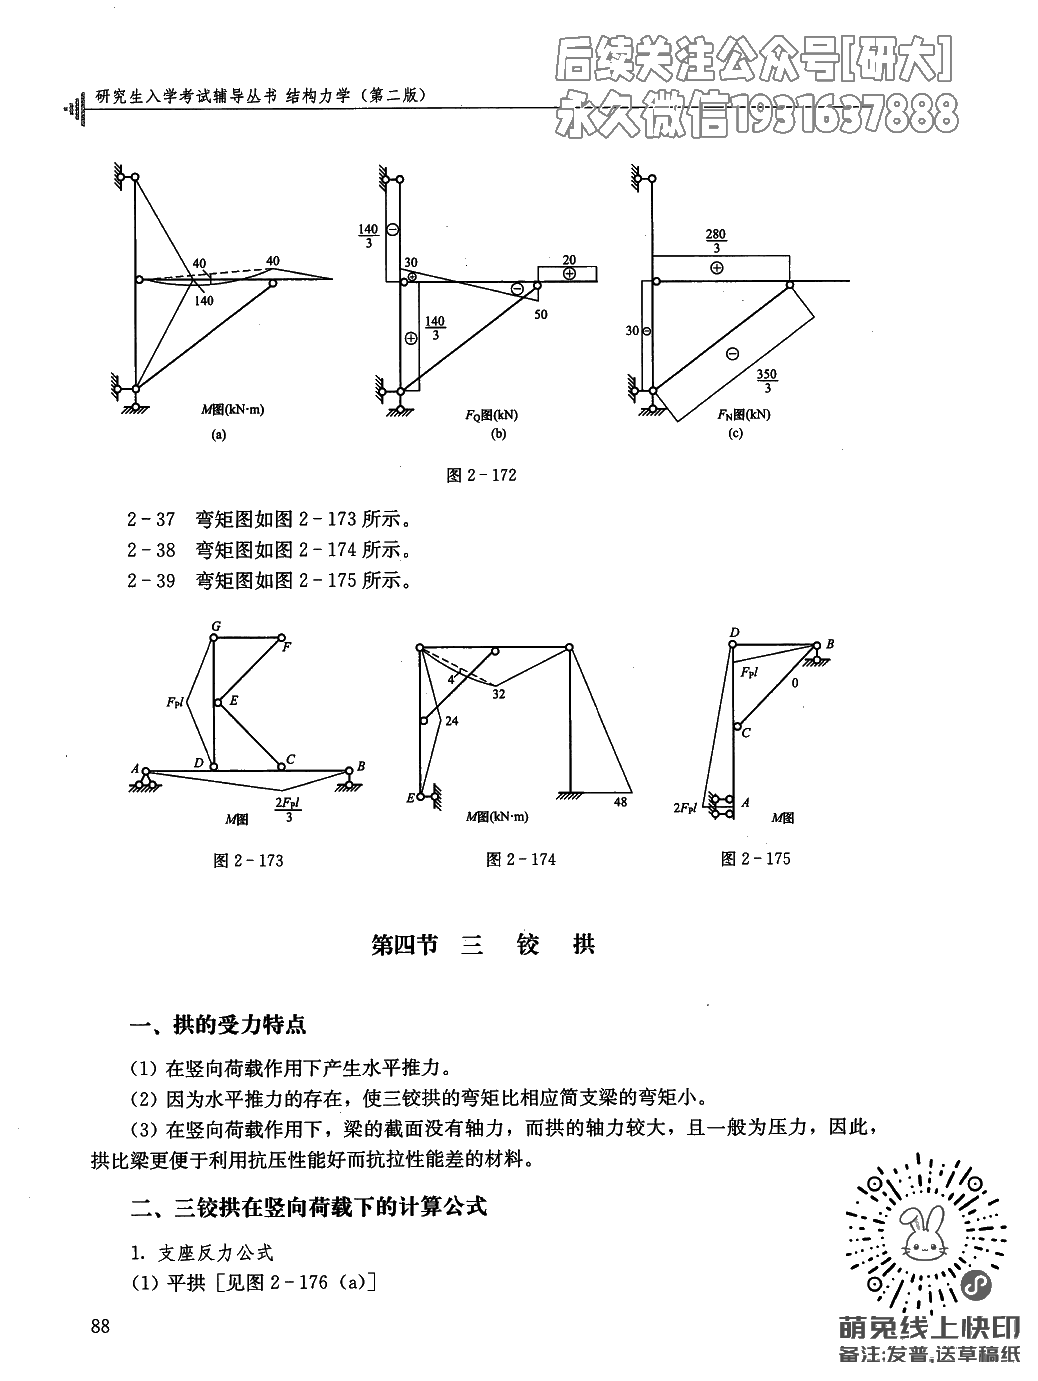
\includegraphics[width=0.96\textwidth,height=0.82\textheight,keepaspectratio]{images/c06_answer_1_p03.png}
\par\small 作业与答案（去水印版），第 3/3 页
\end{center}
\clearpage
\section{讲解笔记（去水印版）}
\begin{center}
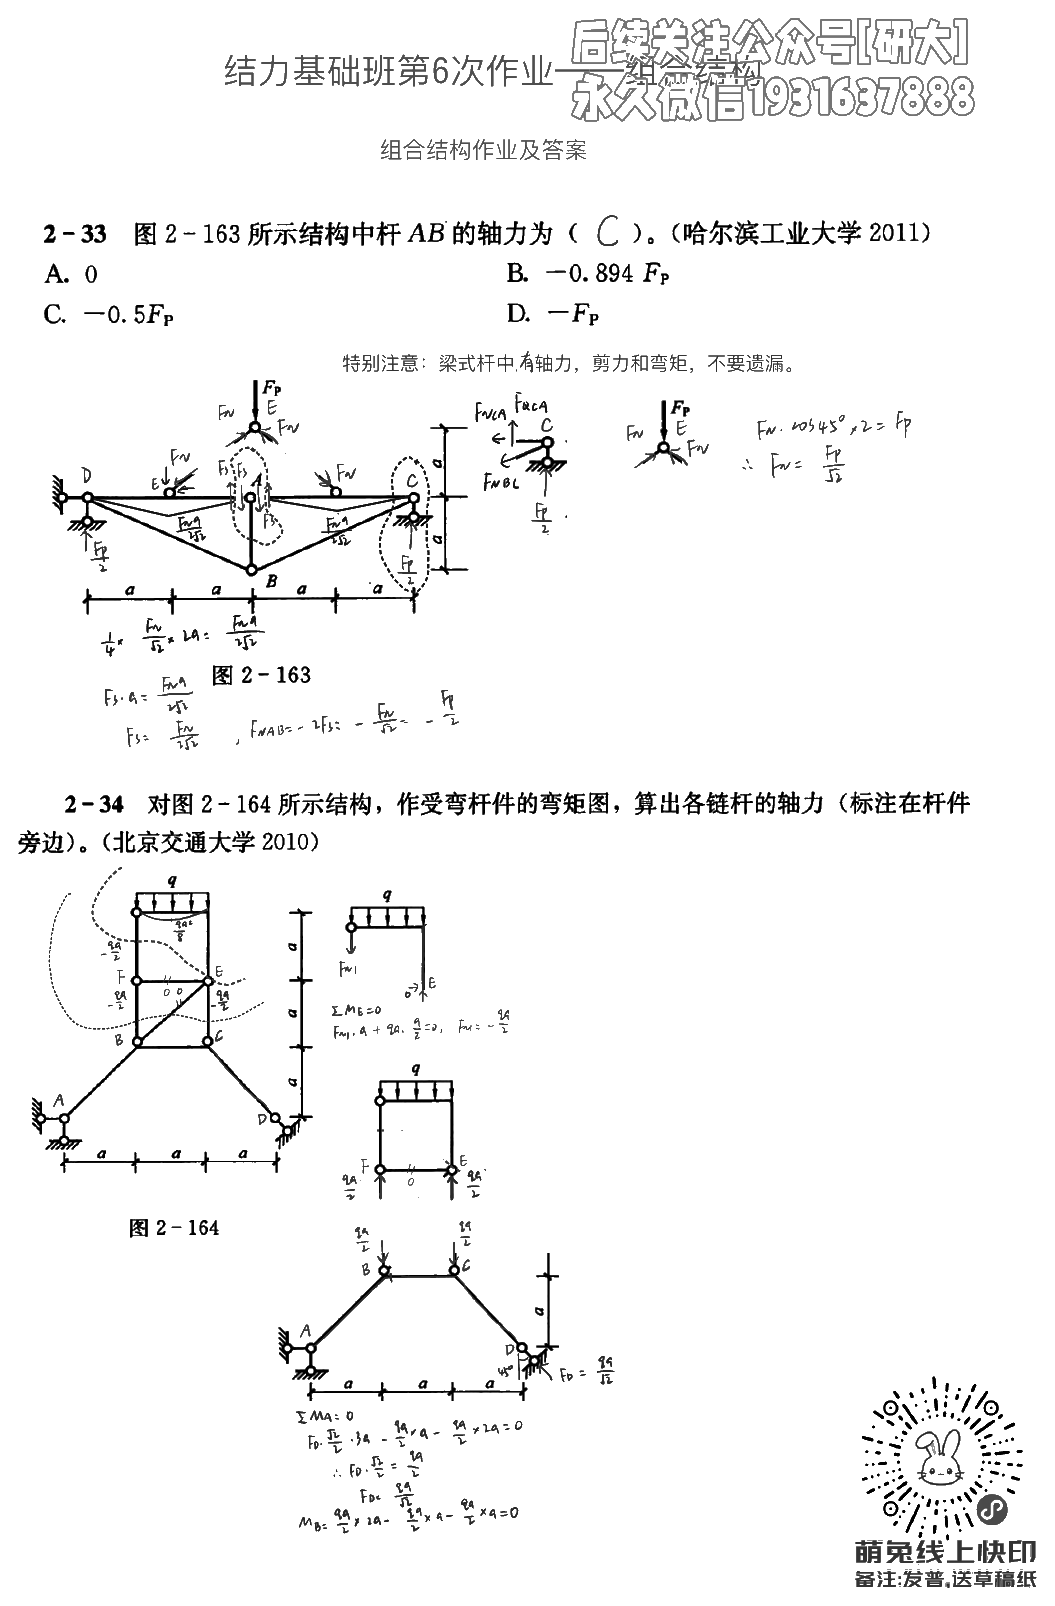
\includegraphics[width=0.96\textwidth,height=0.82\textheight,keepaspectratio]{images/c06_note_p01.png}
\par\small 讲解笔记（去水印版），第 1/6 页
\end{center}
\clearpage
\begin{center}
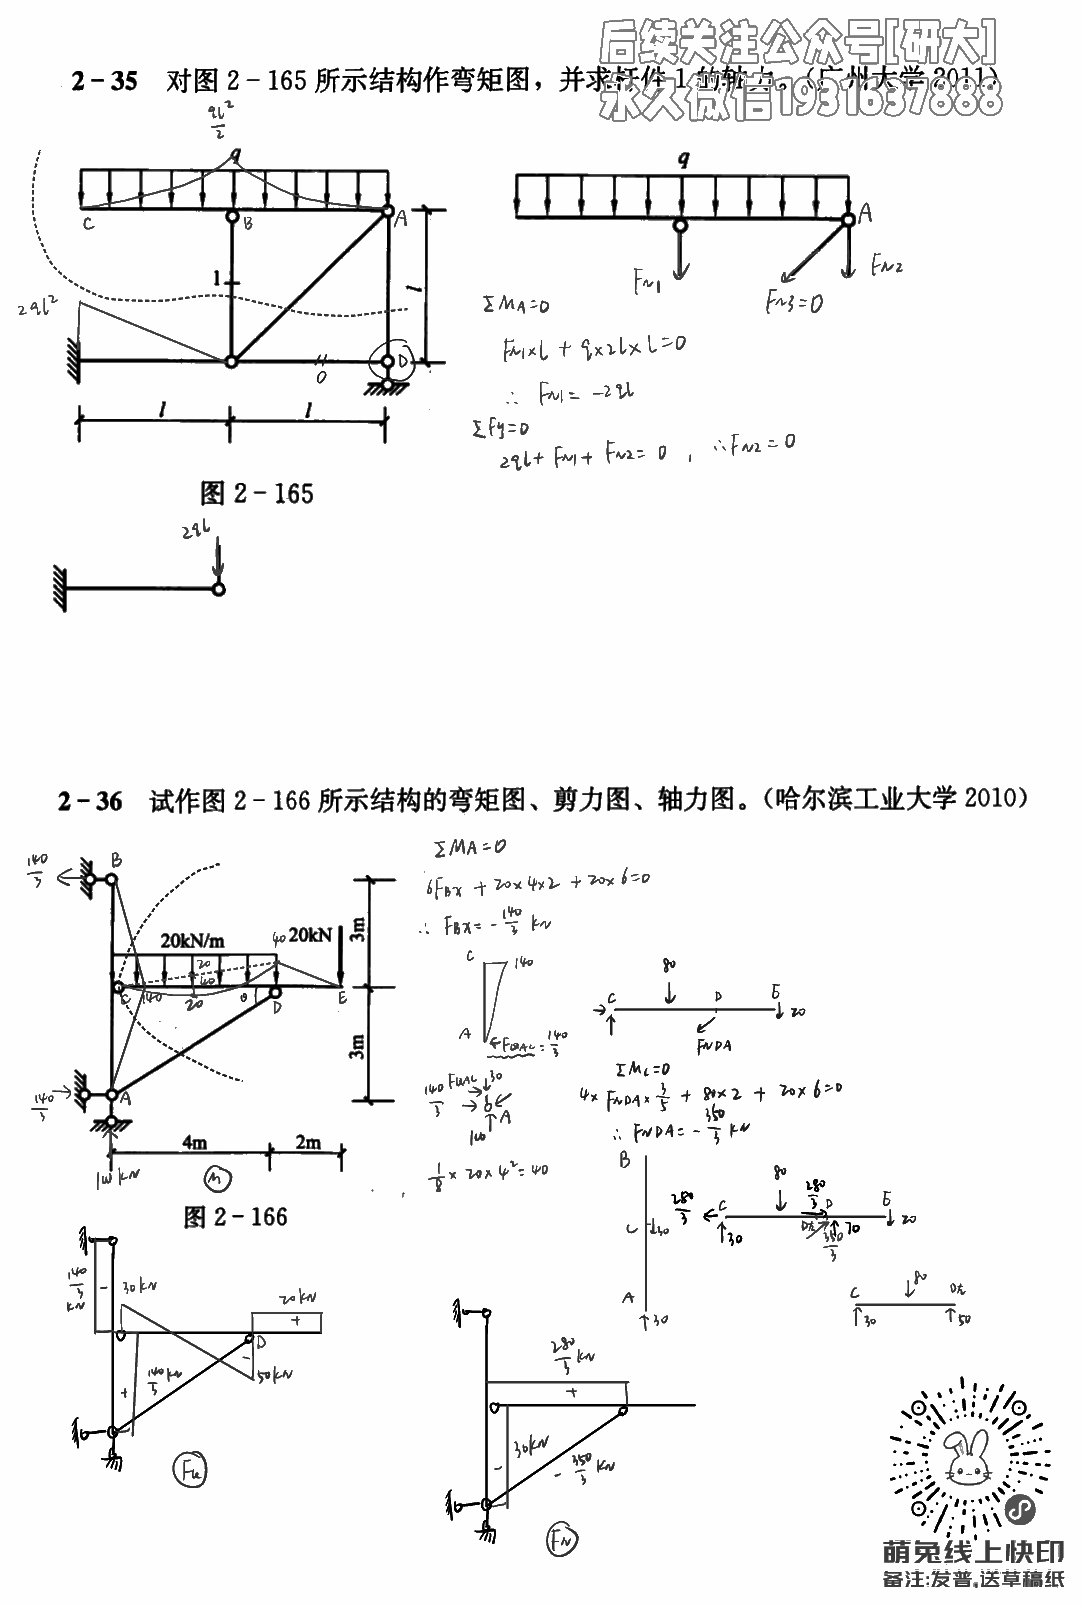
\includegraphics[width=0.96\textwidth,height=0.82\textheight,keepaspectratio]{images/c06_note_p02.png}
\par\small 讲解笔记（去水印版），第 2/6 页
\end{center}
\clearpage
\begin{center}
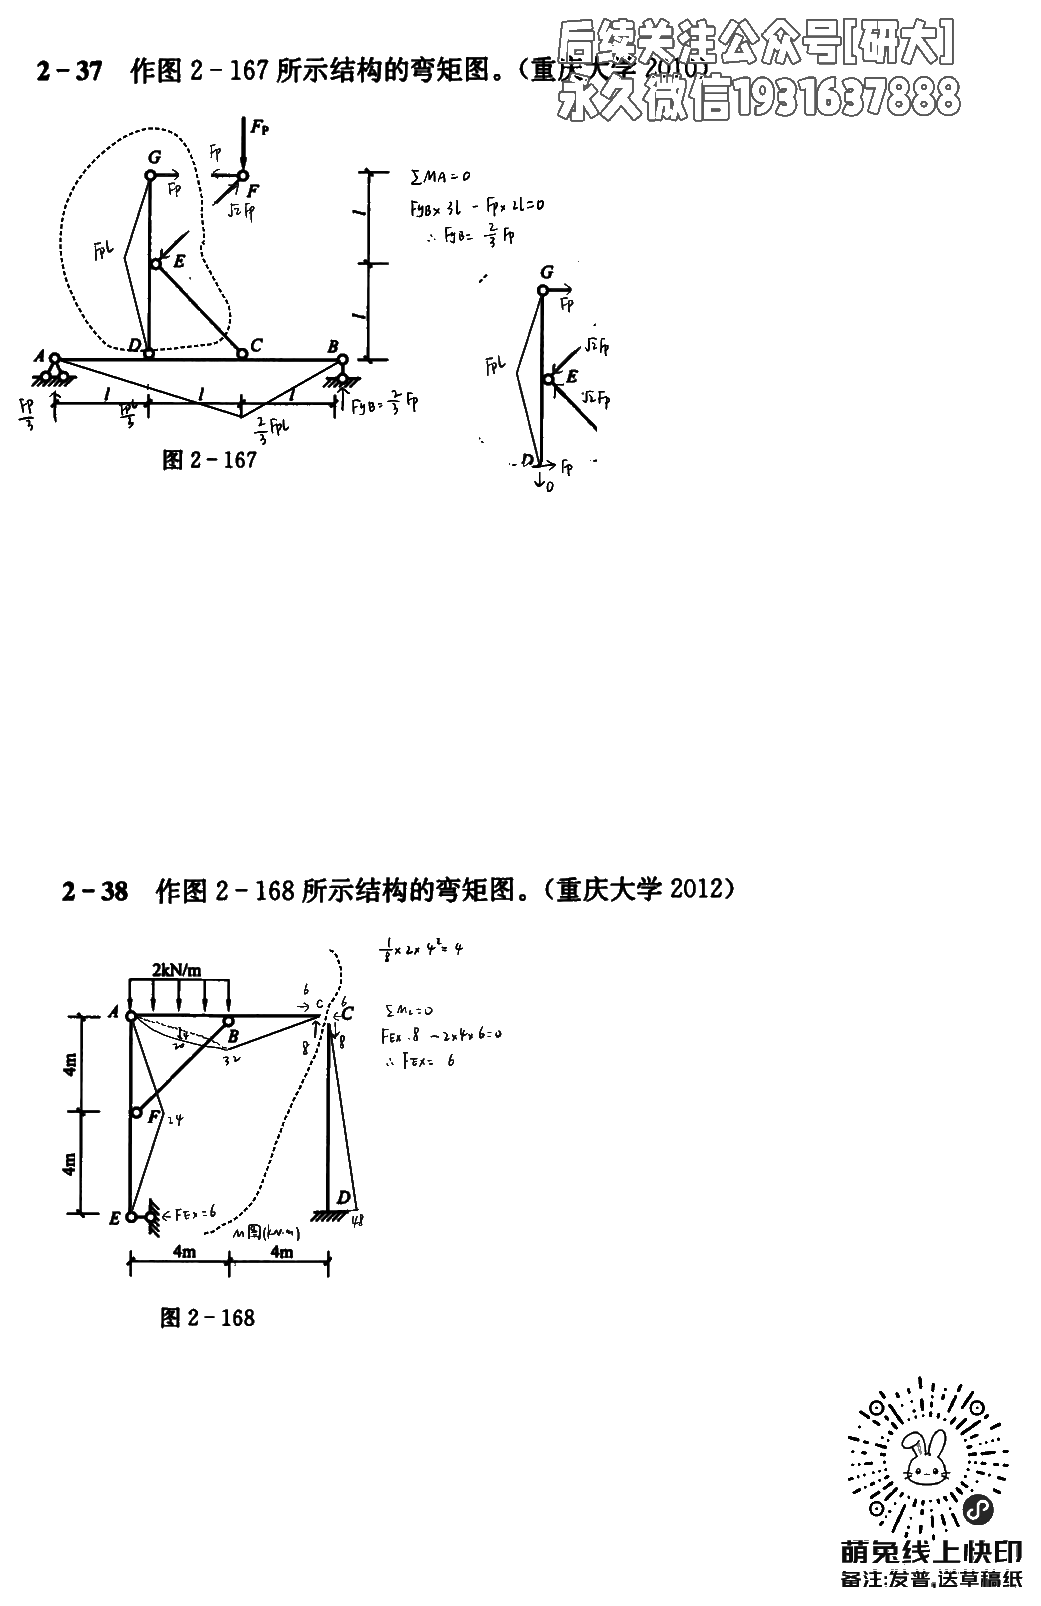
\includegraphics[width=0.96\textwidth,height=0.82\textheight,keepaspectratio]{images/c06_note_p03.png}
\par\small 讲解笔记（去水印版），第 3/6 页
\end{center}
\clearpage
\begin{center}
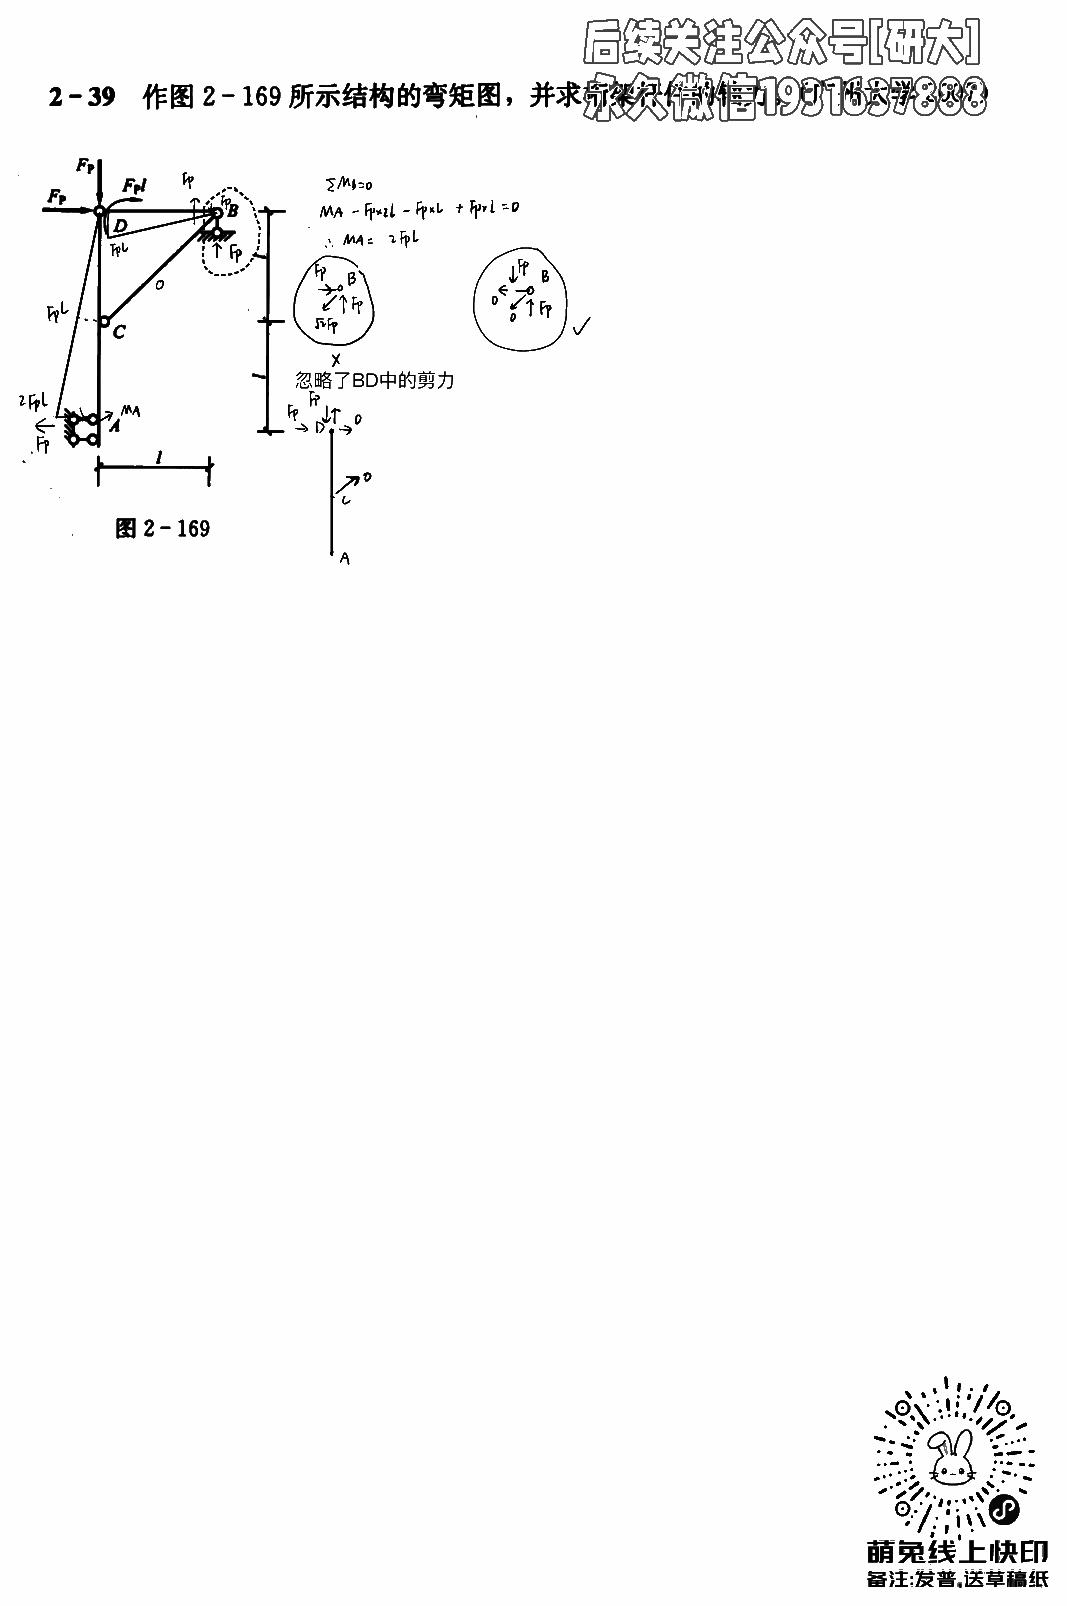
\includegraphics[width=0.96\textwidth,height=0.82\textheight,keepaspectratio]{images/c06_note_p04.png}
\par\small 讲解笔记（去水印版），第 4/6 页
\end{center}
\clearpage
\begin{center}
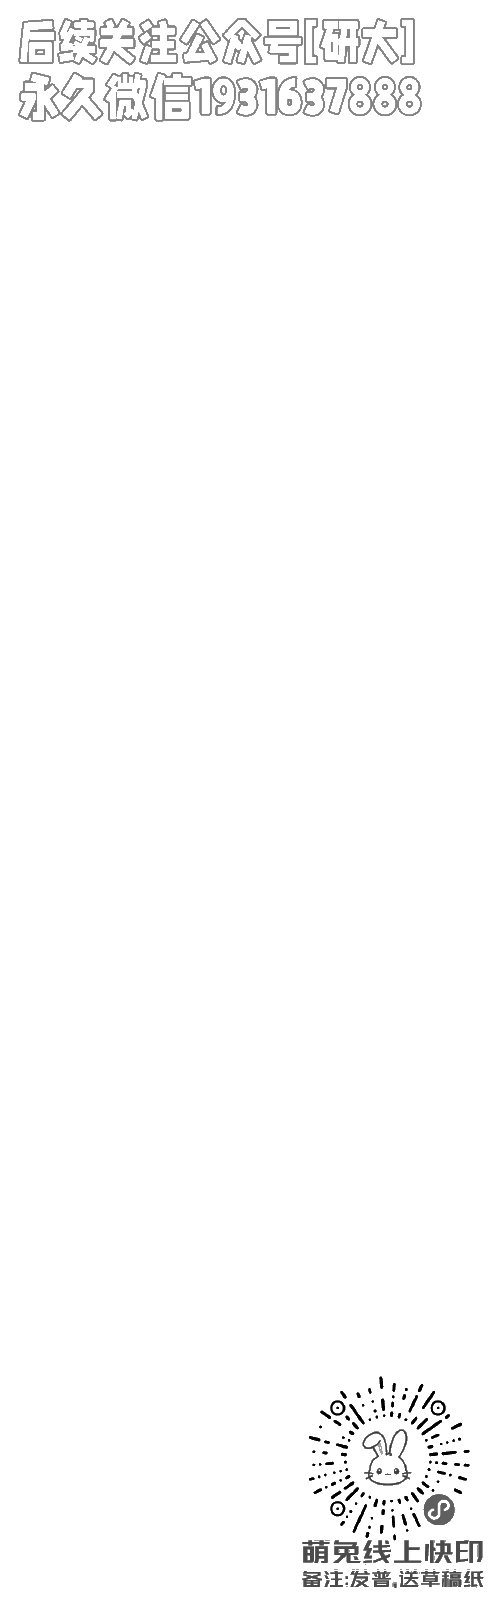
\includegraphics[width=0.96\textwidth,height=0.82\textheight,keepaspectratio]{images/c06_note_p05.png}
\par\small 讲解笔记（去水印版），第 5/6 页
\end{center}
\clearpage
\begin{center}
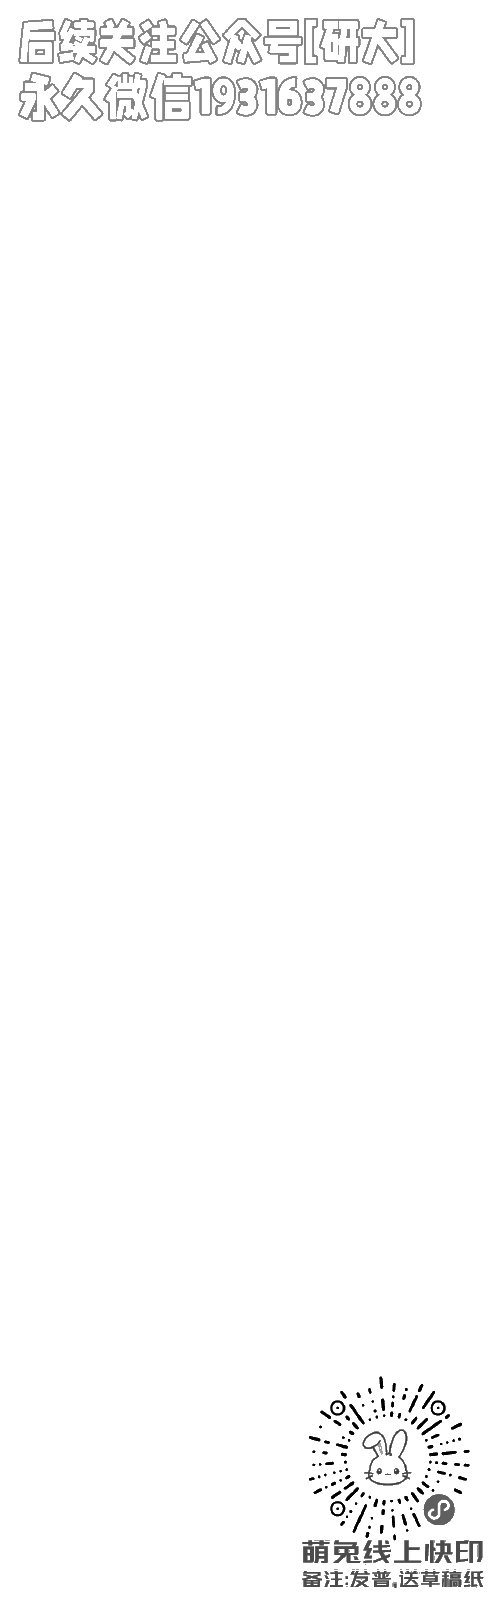
\includegraphics[width=0.96\textwidth,height=0.82\textheight,keepaspectratio]{images/c06_note_p06.png}
\par\small 讲解笔记（去水印版），第 6/6 页
\end{center}
\clearpage
\chapter{第7讲：三铰拱}
\begin{tcolorbox}[title=解析要点]
三铰拱利用整体平衡和中间铰弯矩为零求水平推力。任意截面内力可由左段或右段隔离体求得，并与同跨度简支梁弯矩关系校核。
\end{tcolorbox}
\begin{tcolorbox}[title=答案与校核]
答案页给出三铰拱水平推力和截面内力；中铰弯矩为零可作为核心校核。
\end{tcolorbox}
\section{作业与答案（去水印版）}
\begin{center}
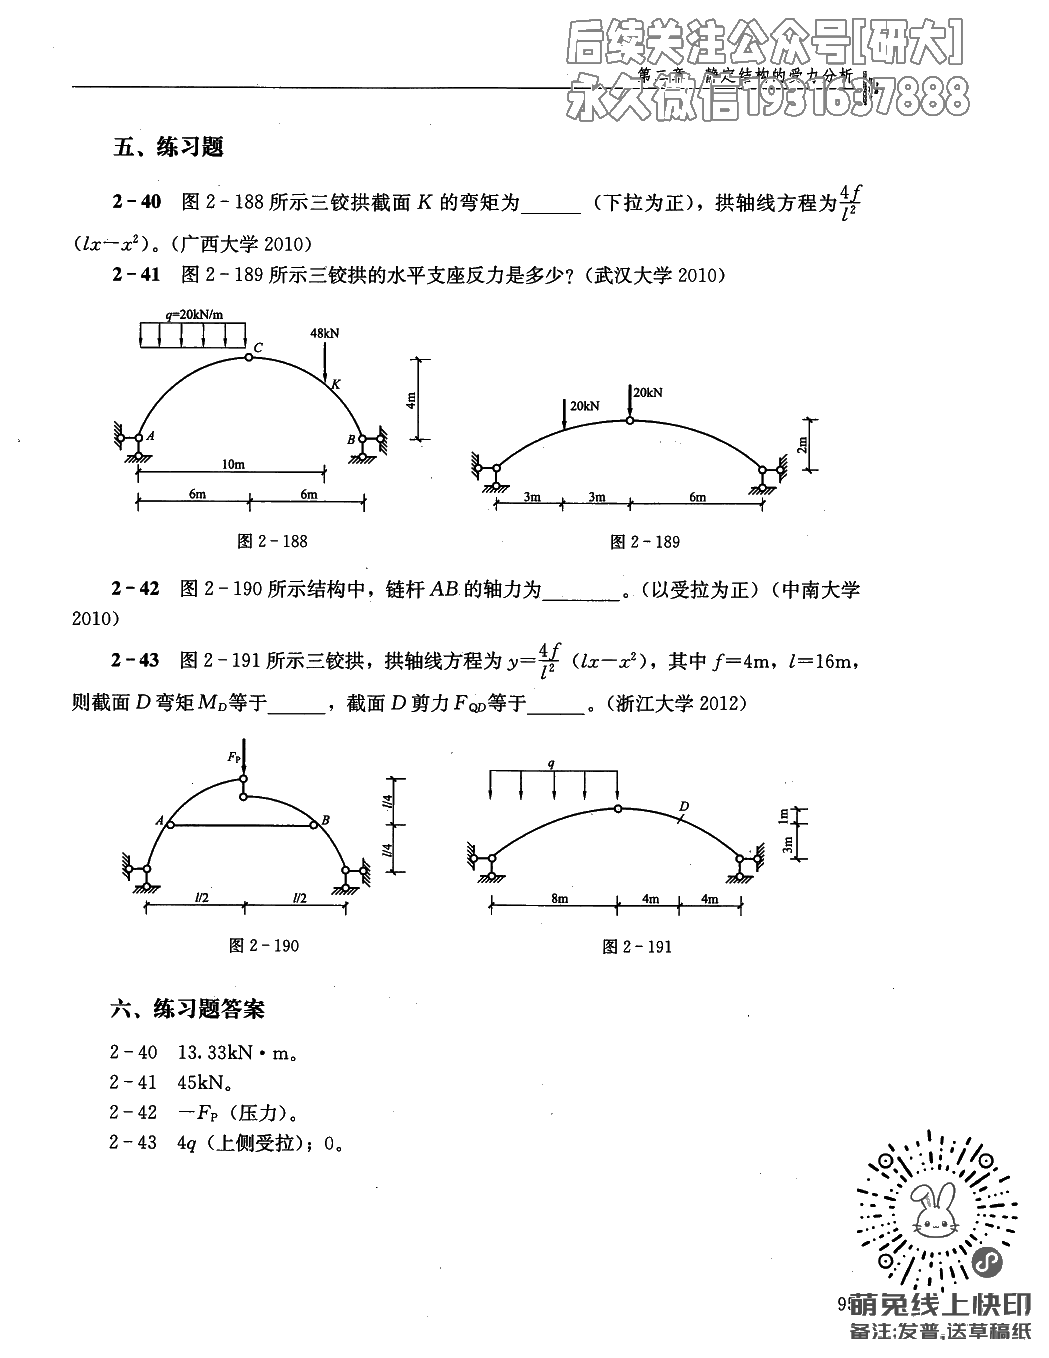
\includegraphics[width=0.96\textwidth,height=0.82\textheight,keepaspectratio]{images/c07_answer_1_p01.png}
\par\small 作业与答案（去水印版），第 1/1 页
\end{center}
\clearpage
\section{讲解笔记（去水印版）}
\begin{center}
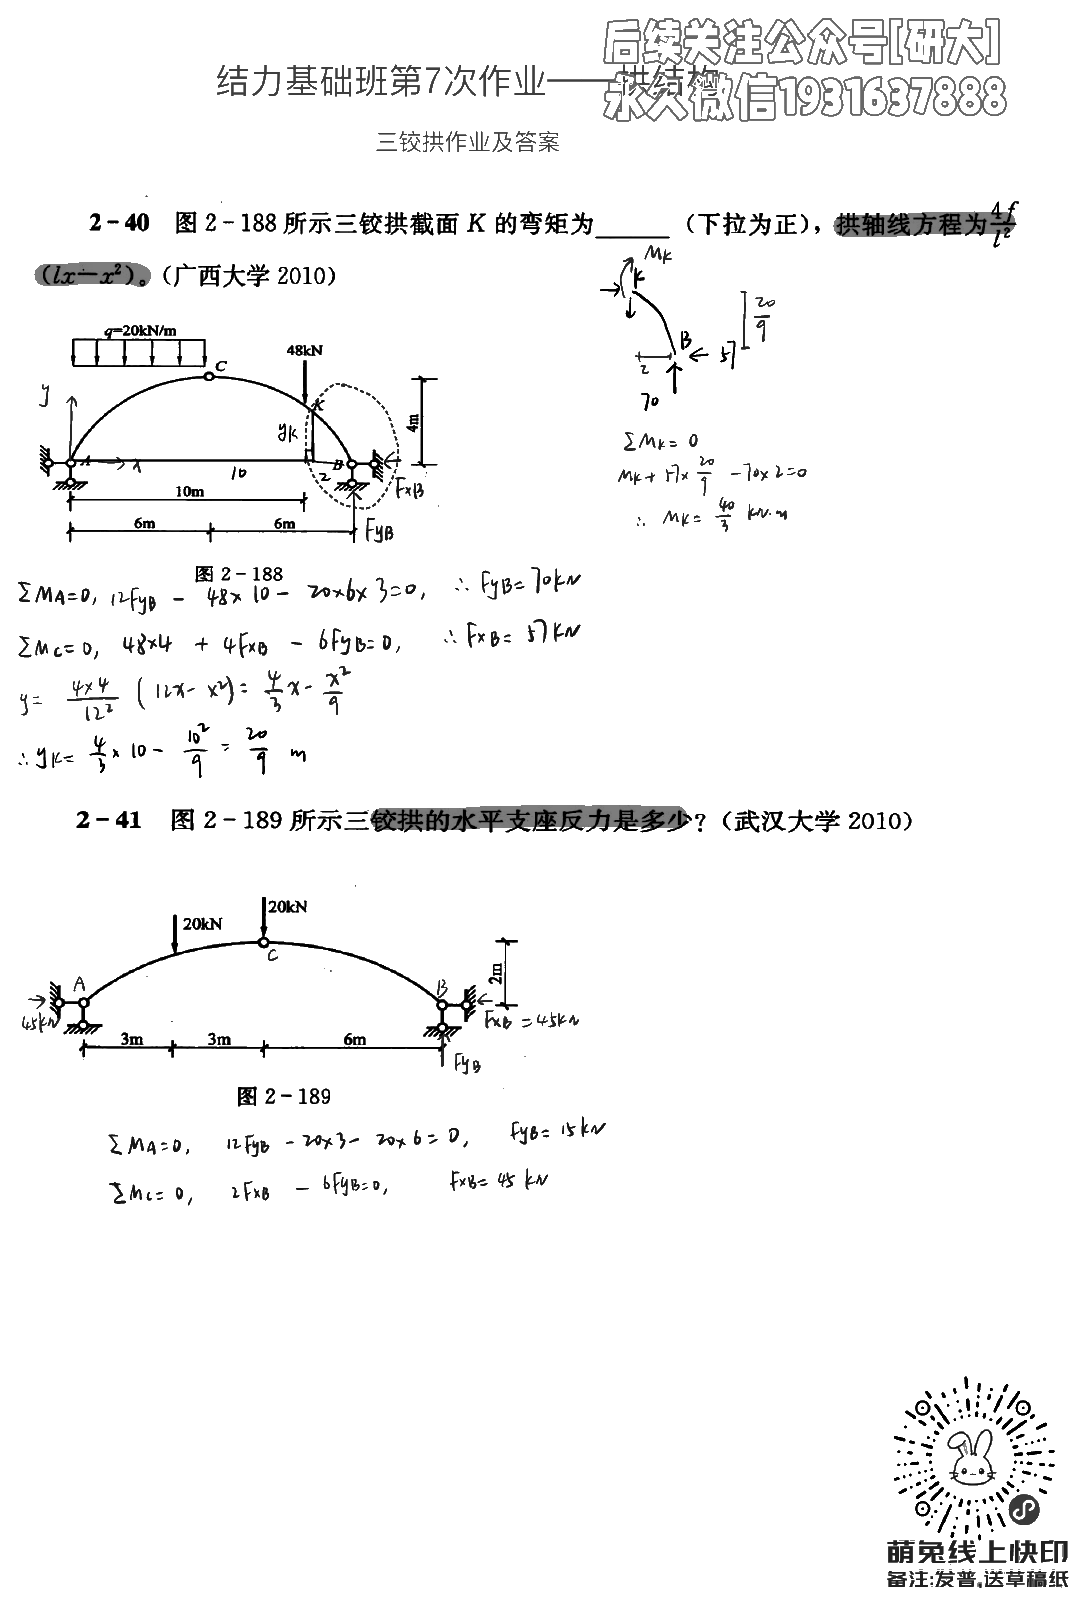
\includegraphics[width=0.96\textwidth,height=0.82\textheight,keepaspectratio]{images/c07_note_p01.png}
\par\small 讲解笔记（去水印版），第 1/2 页
\end{center}
\clearpage
\begin{center}
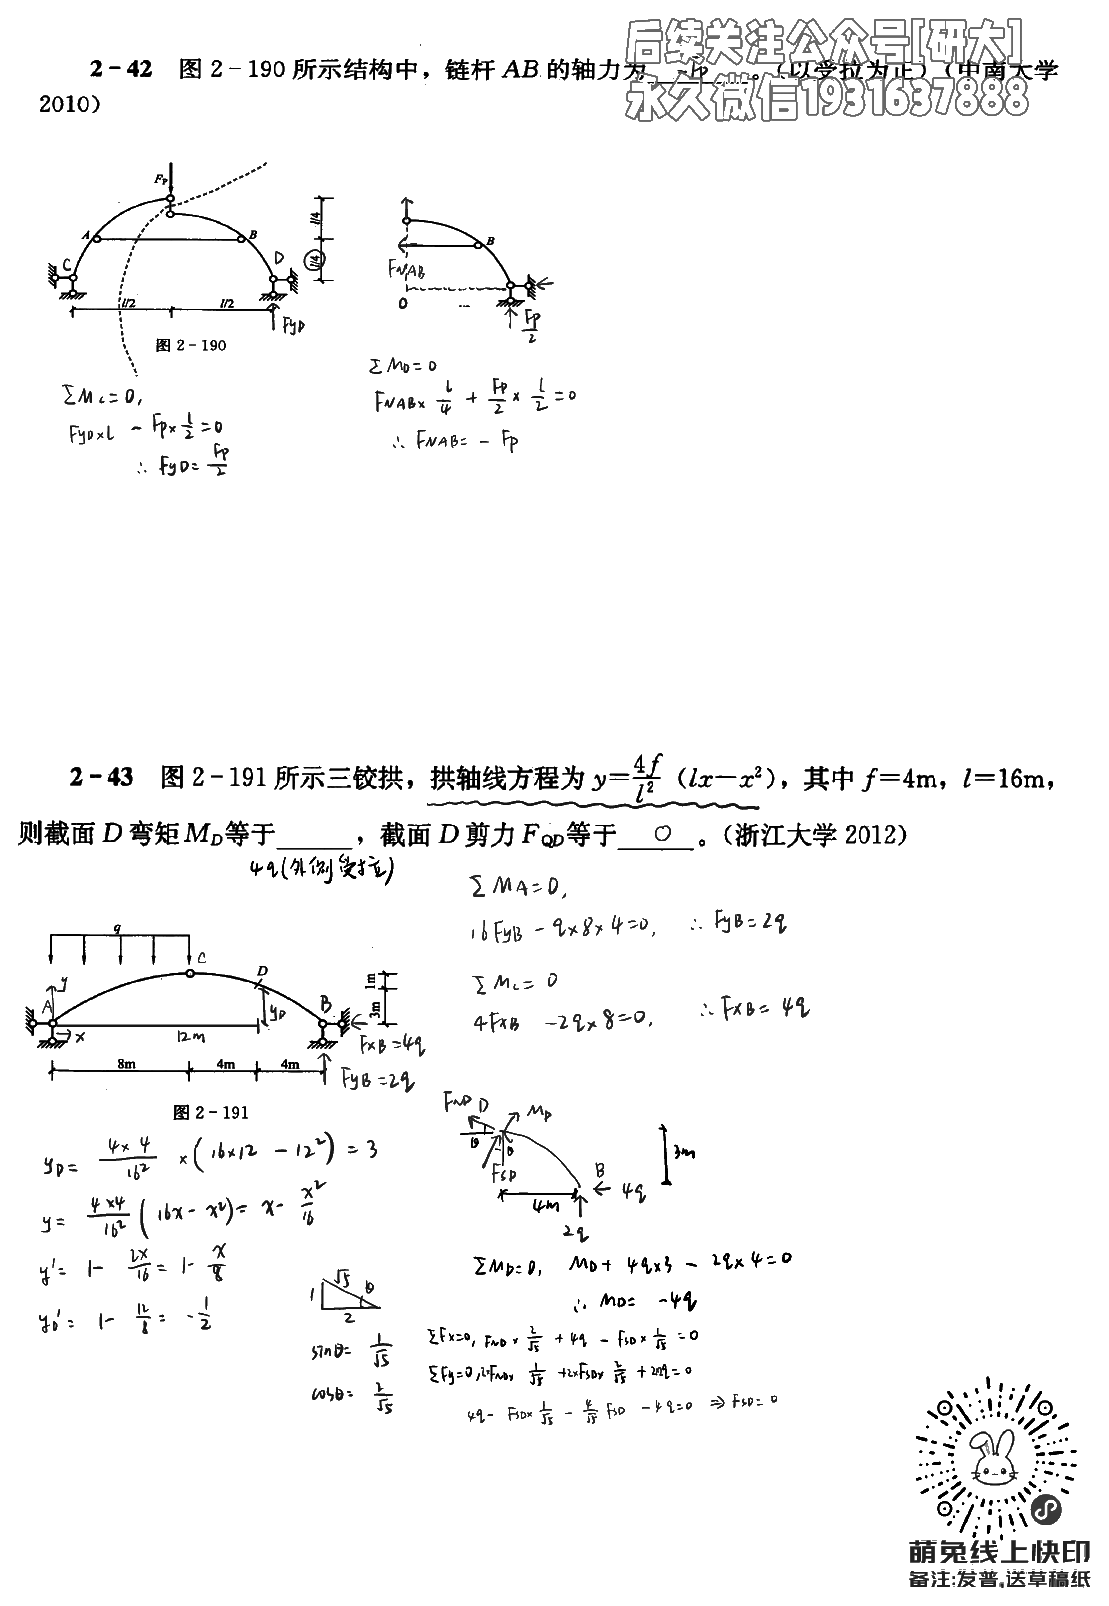
\includegraphics[width=0.96\textwidth,height=0.82\textheight,keepaspectratio]{images/c07_note_p02.png}
\par\small 讲解笔记（去水印版），第 2/2 页
\end{center}
\clearpage
\chapter{第8讲：静定结构影响线}
\begin{tcolorbox}[title=解析要点]
影响线可用静力法或机动法。反力影响线来自单位移动荷载平衡，剪力和弯矩影响线要明确考察截面左右侧取隔离体。
\end{tcolorbox}
\begin{tcolorbox}[title=答案与校核]
答案页给出影响线图和关键纵坐标；应检查单位荷载在控制位置时的正负号。
\end{tcolorbox}
\section{作业与答案（去水印版）}
\begin{center}
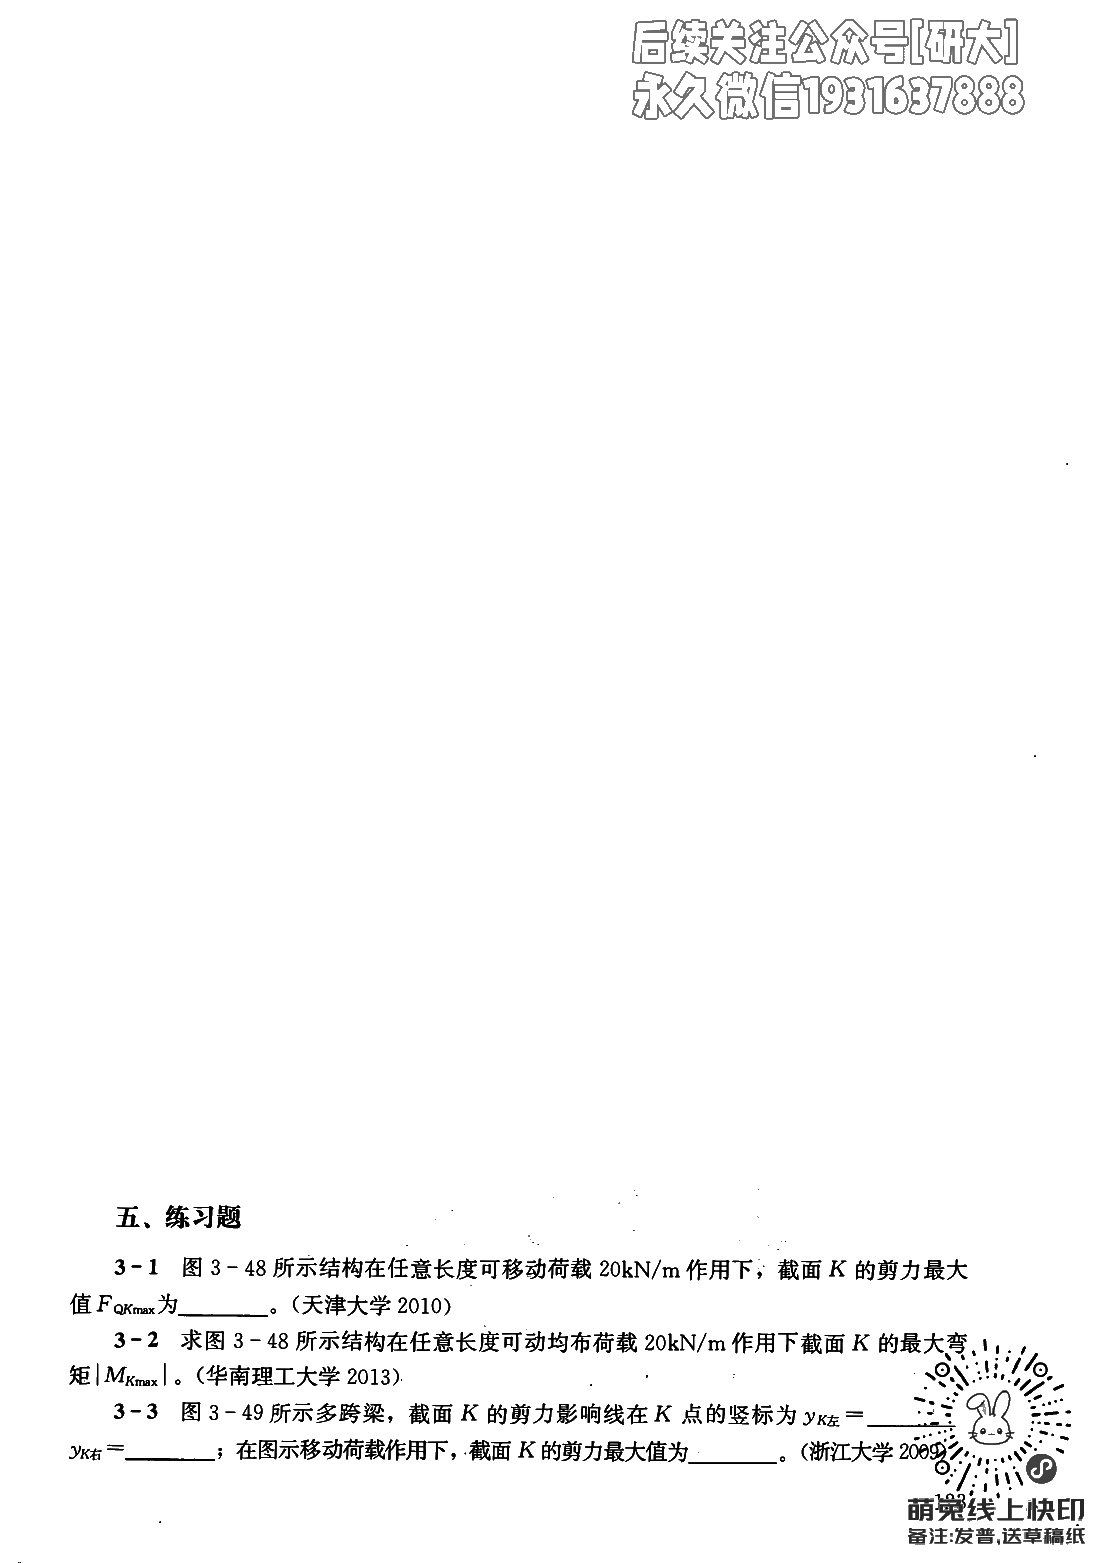
\includegraphics[width=0.96\textwidth,height=0.82\textheight,keepaspectratio]{images/c08_answer_1_p01.png}
\par\small 作业与答案（去水印版），第 1/18 页
\end{center}
\clearpage
\begin{center}
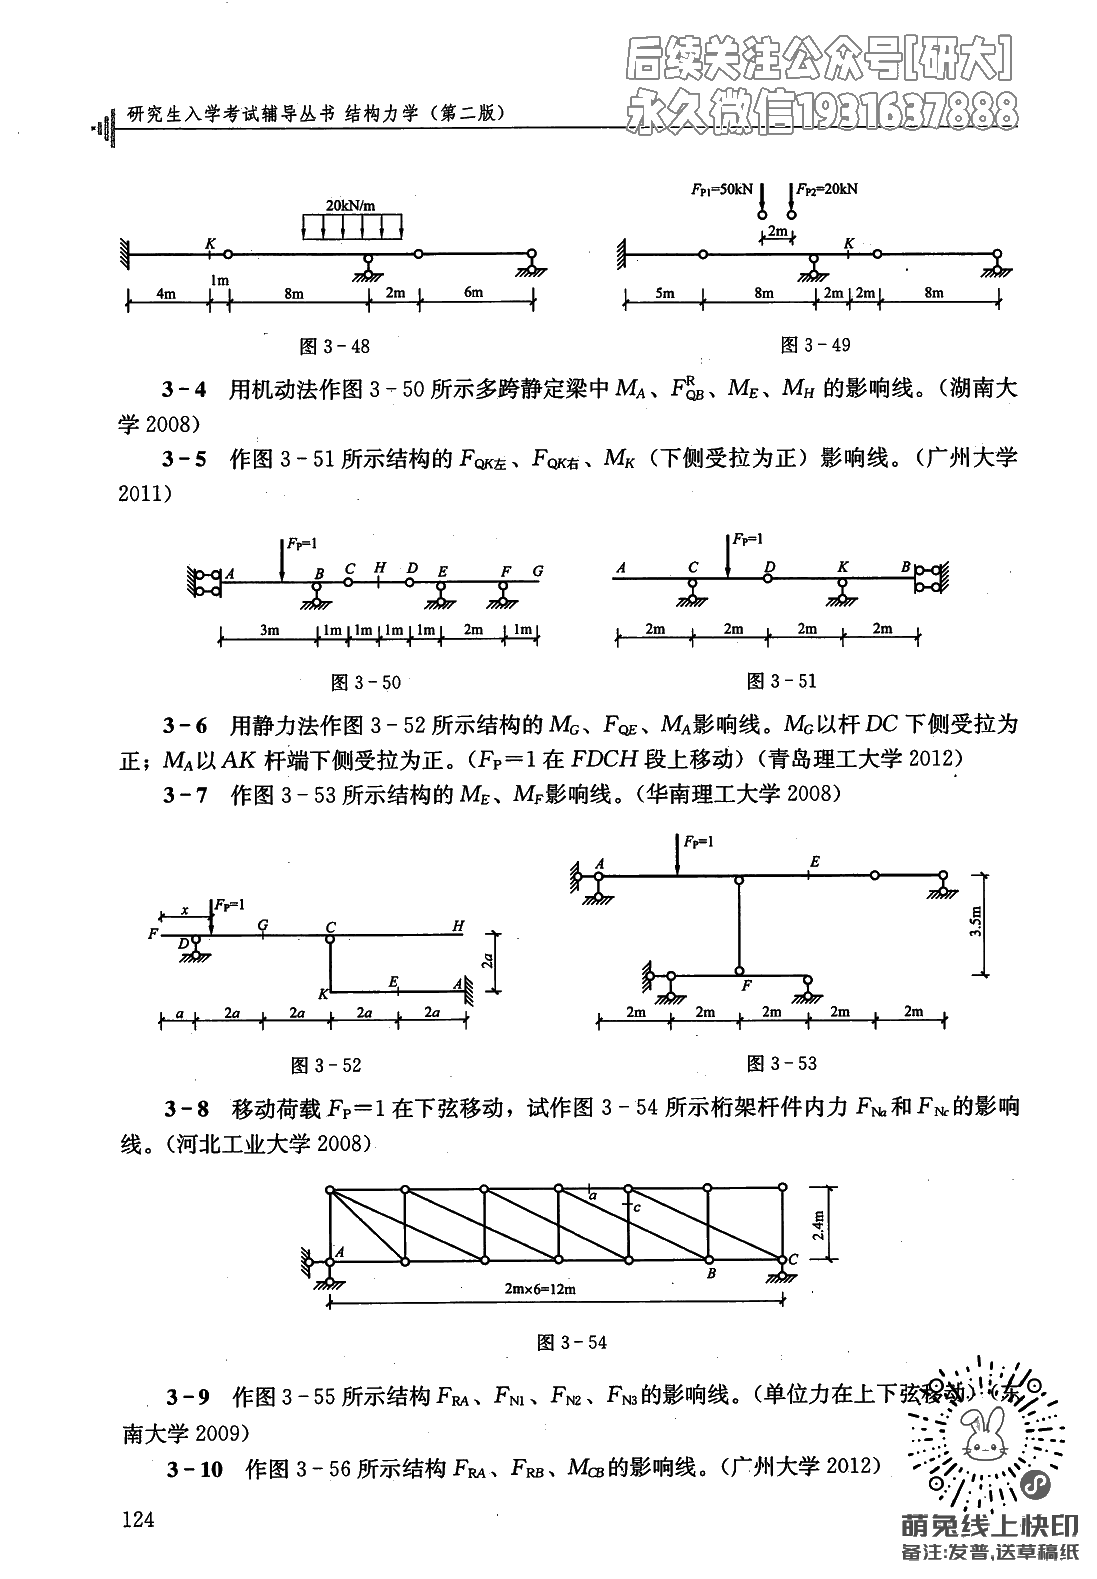
\includegraphics[width=0.96\textwidth,height=0.82\textheight,keepaspectratio]{images/c08_answer_1_p02.png}
\par\small 作业与答案（去水印版），第 2/18 页
\end{center}
\clearpage
\begin{center}
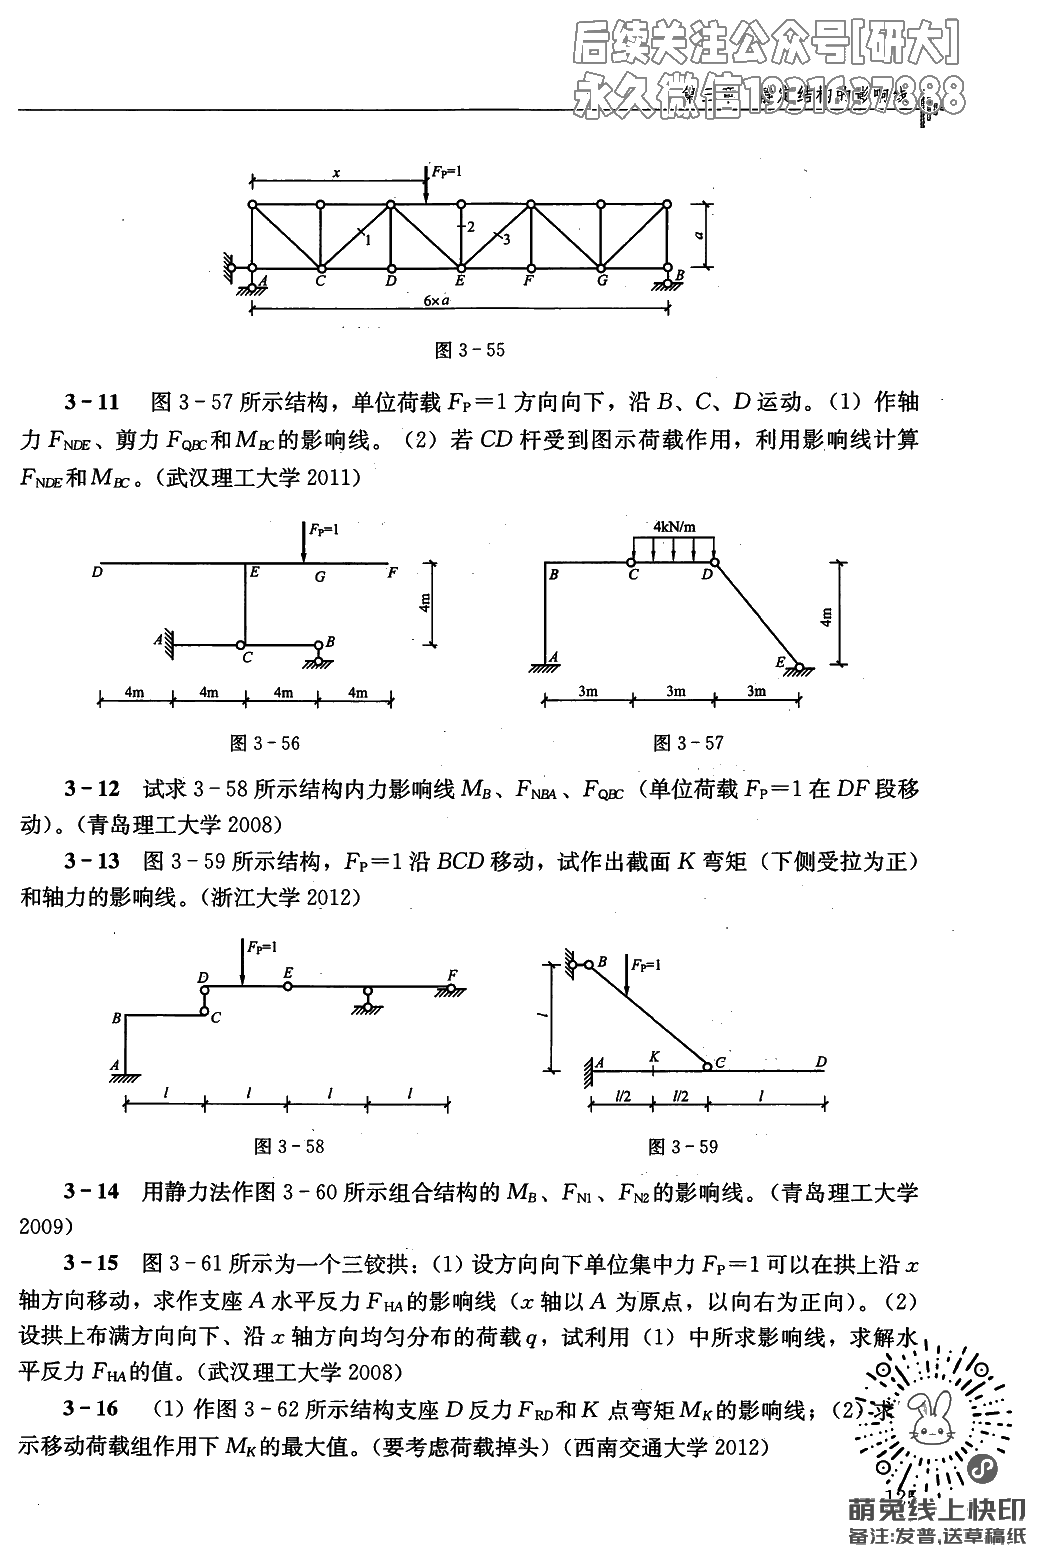
\includegraphics[width=0.96\textwidth,height=0.82\textheight,keepaspectratio]{images/c08_answer_1_p03.png}
\par\small 作业与答案（去水印版），第 3/18 页
\end{center}
\clearpage
\begin{center}
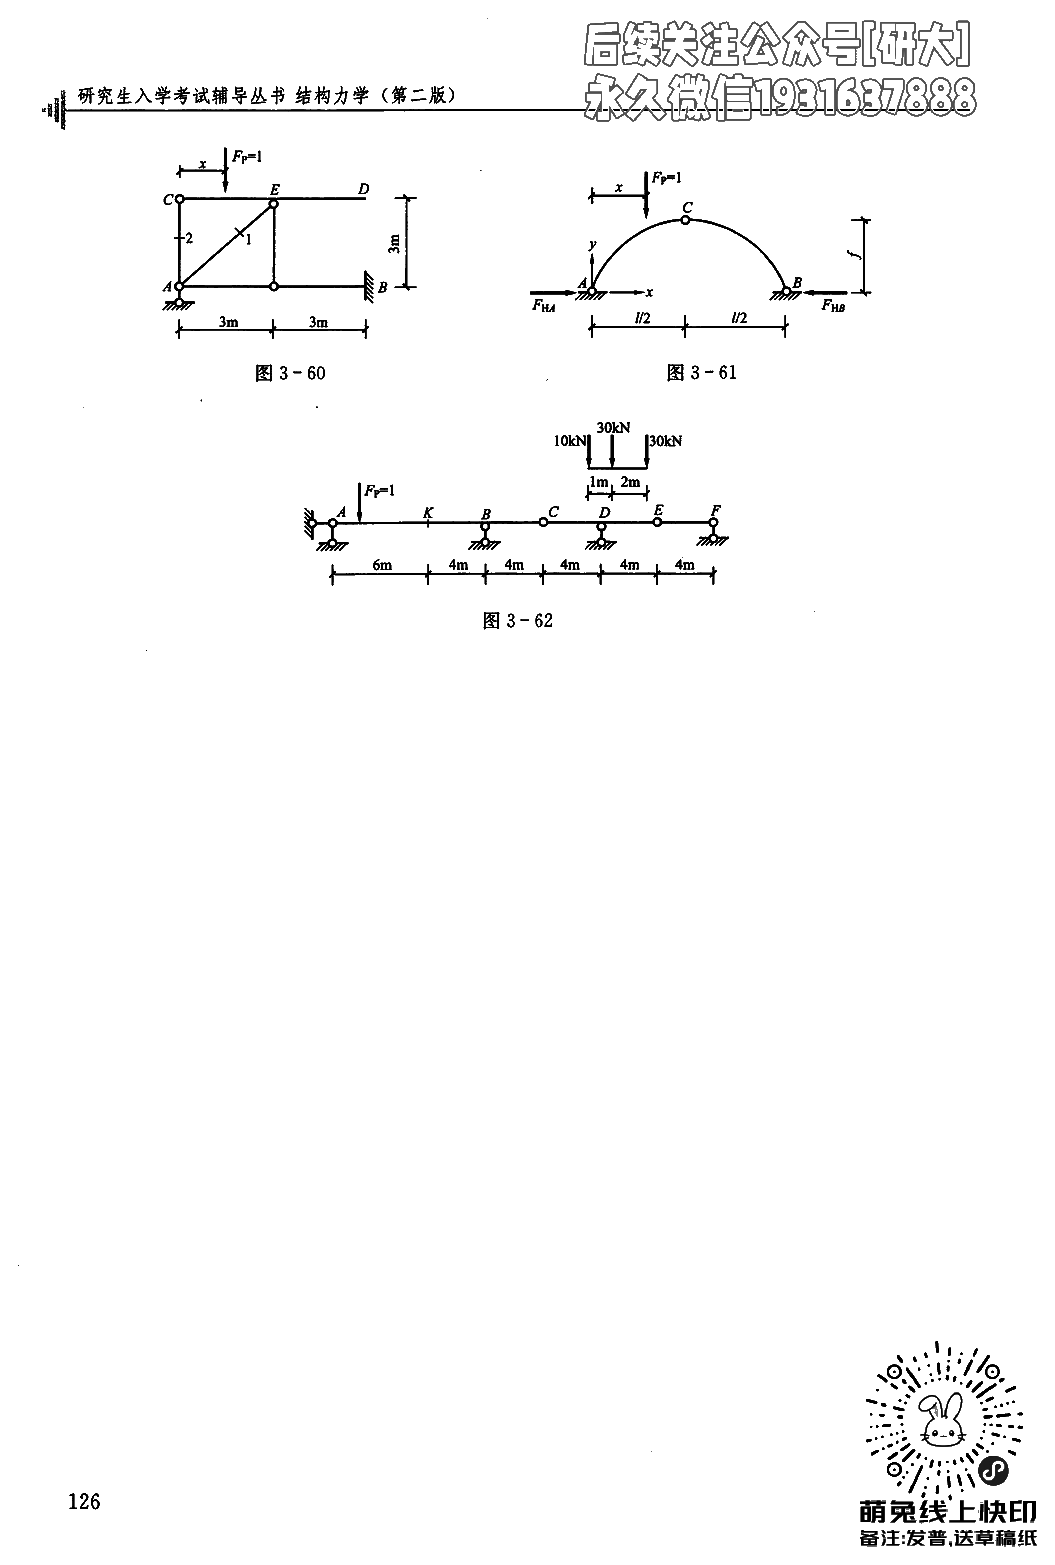
\includegraphics[width=0.96\textwidth,height=0.82\textheight,keepaspectratio]{images/c08_answer_1_p04.png}
\par\small 作业与答案（去水印版），第 4/18 页
\end{center}
\clearpage
\begin{center}
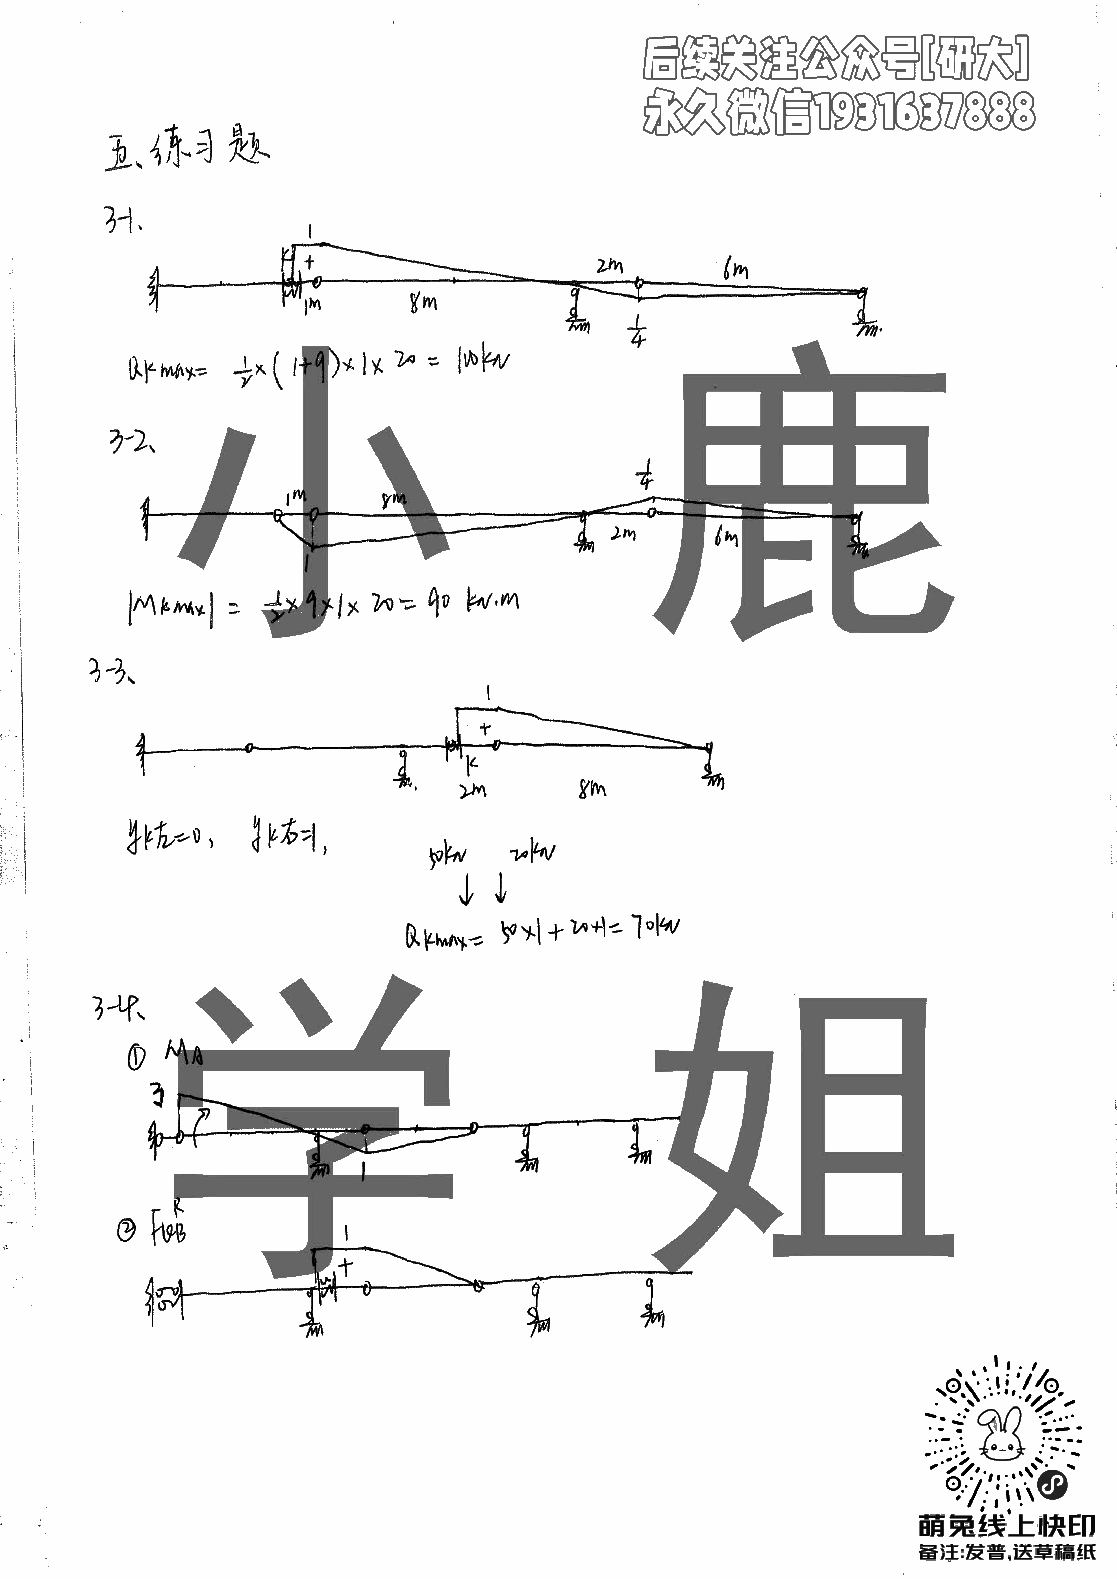
\includegraphics[width=0.96\textwidth,height=0.82\textheight,keepaspectratio]{images/c08_answer_1_p05.png}
\par\small 作业与答案（去水印版），第 5/18 页
\end{center}
\clearpage
\begin{center}
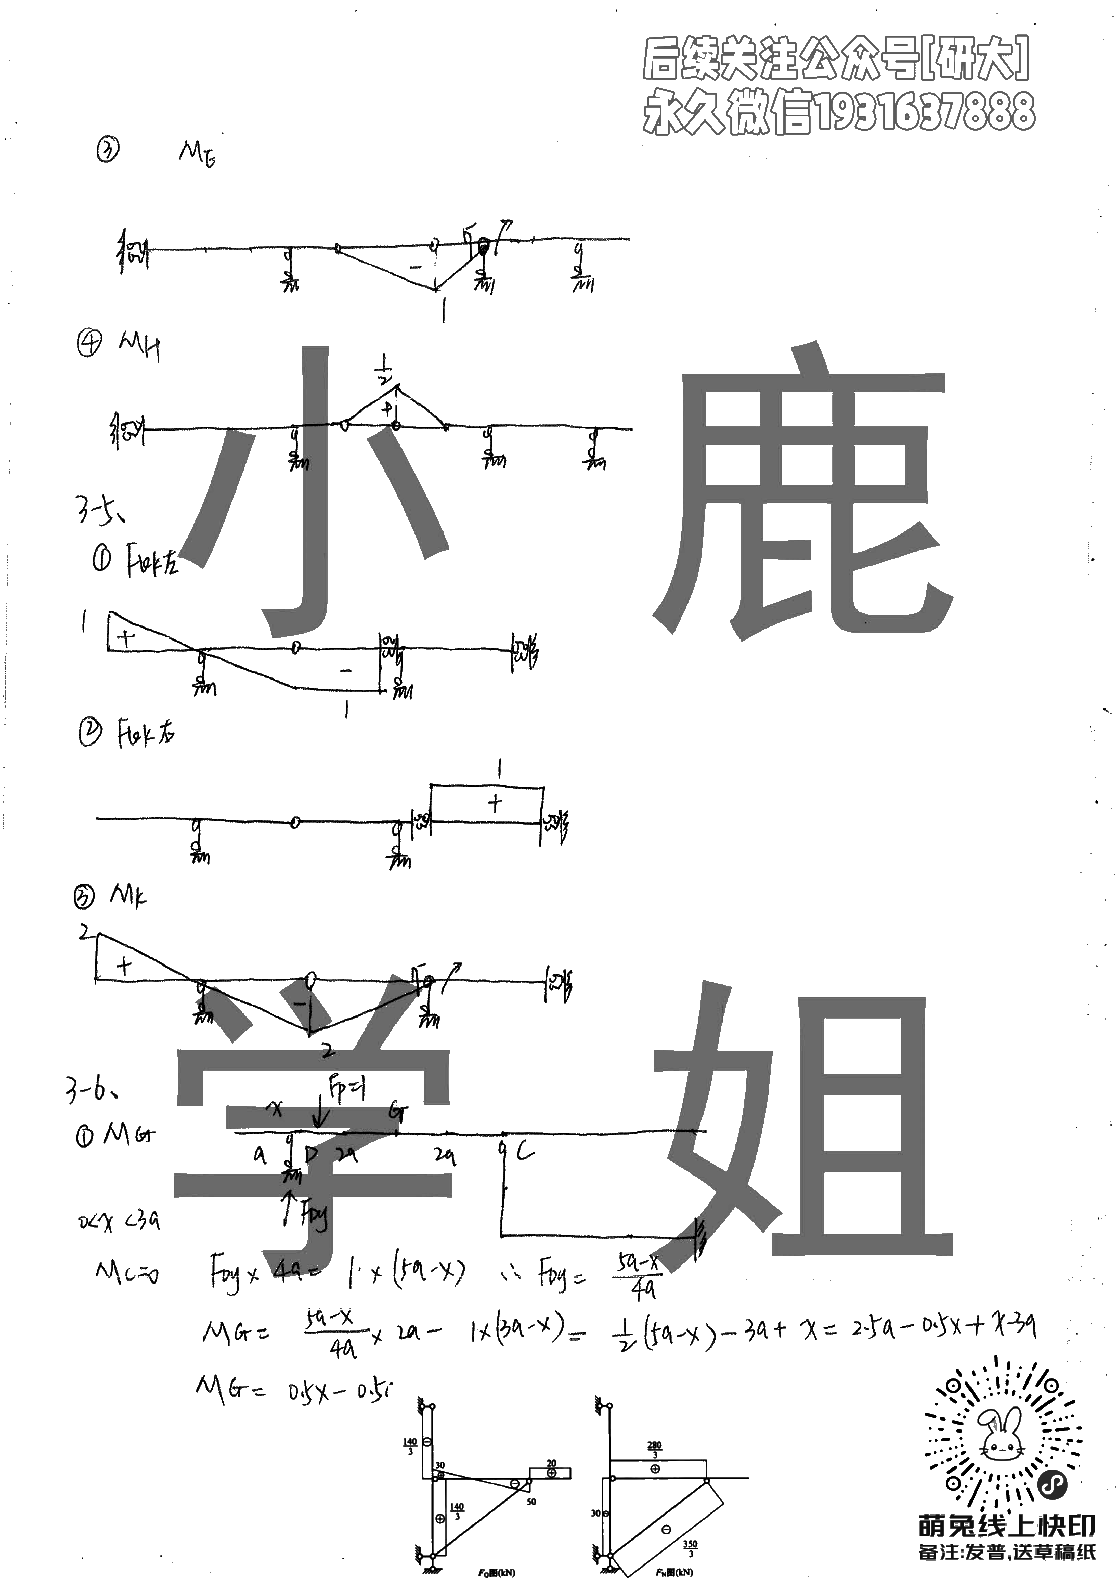
\includegraphics[width=0.96\textwidth,height=0.82\textheight,keepaspectratio]{images/c08_answer_1_p06.png}
\par\small 作业与答案（去水印版），第 6/18 页
\end{center}
\clearpage
\begin{center}
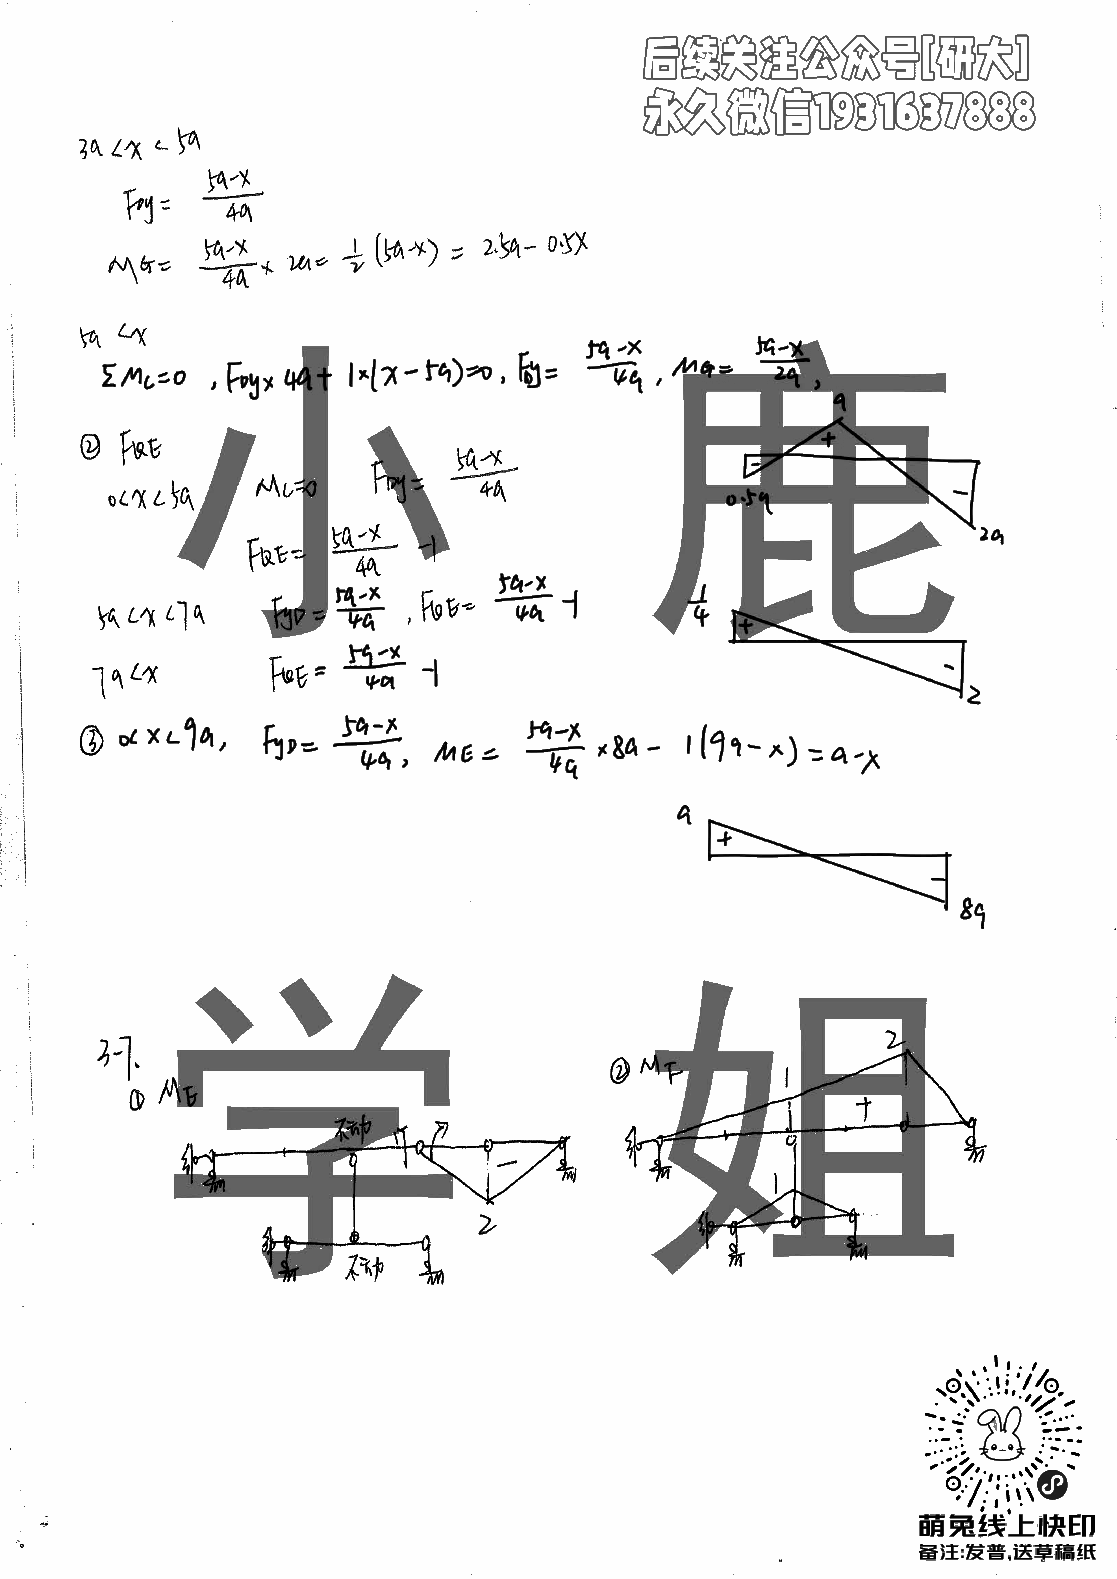
\includegraphics[width=0.96\textwidth,height=0.82\textheight,keepaspectratio]{images/c08_answer_1_p07.png}
\par\small 作业与答案（去水印版），第 7/18 页
\end{center}
\clearpage
\begin{center}
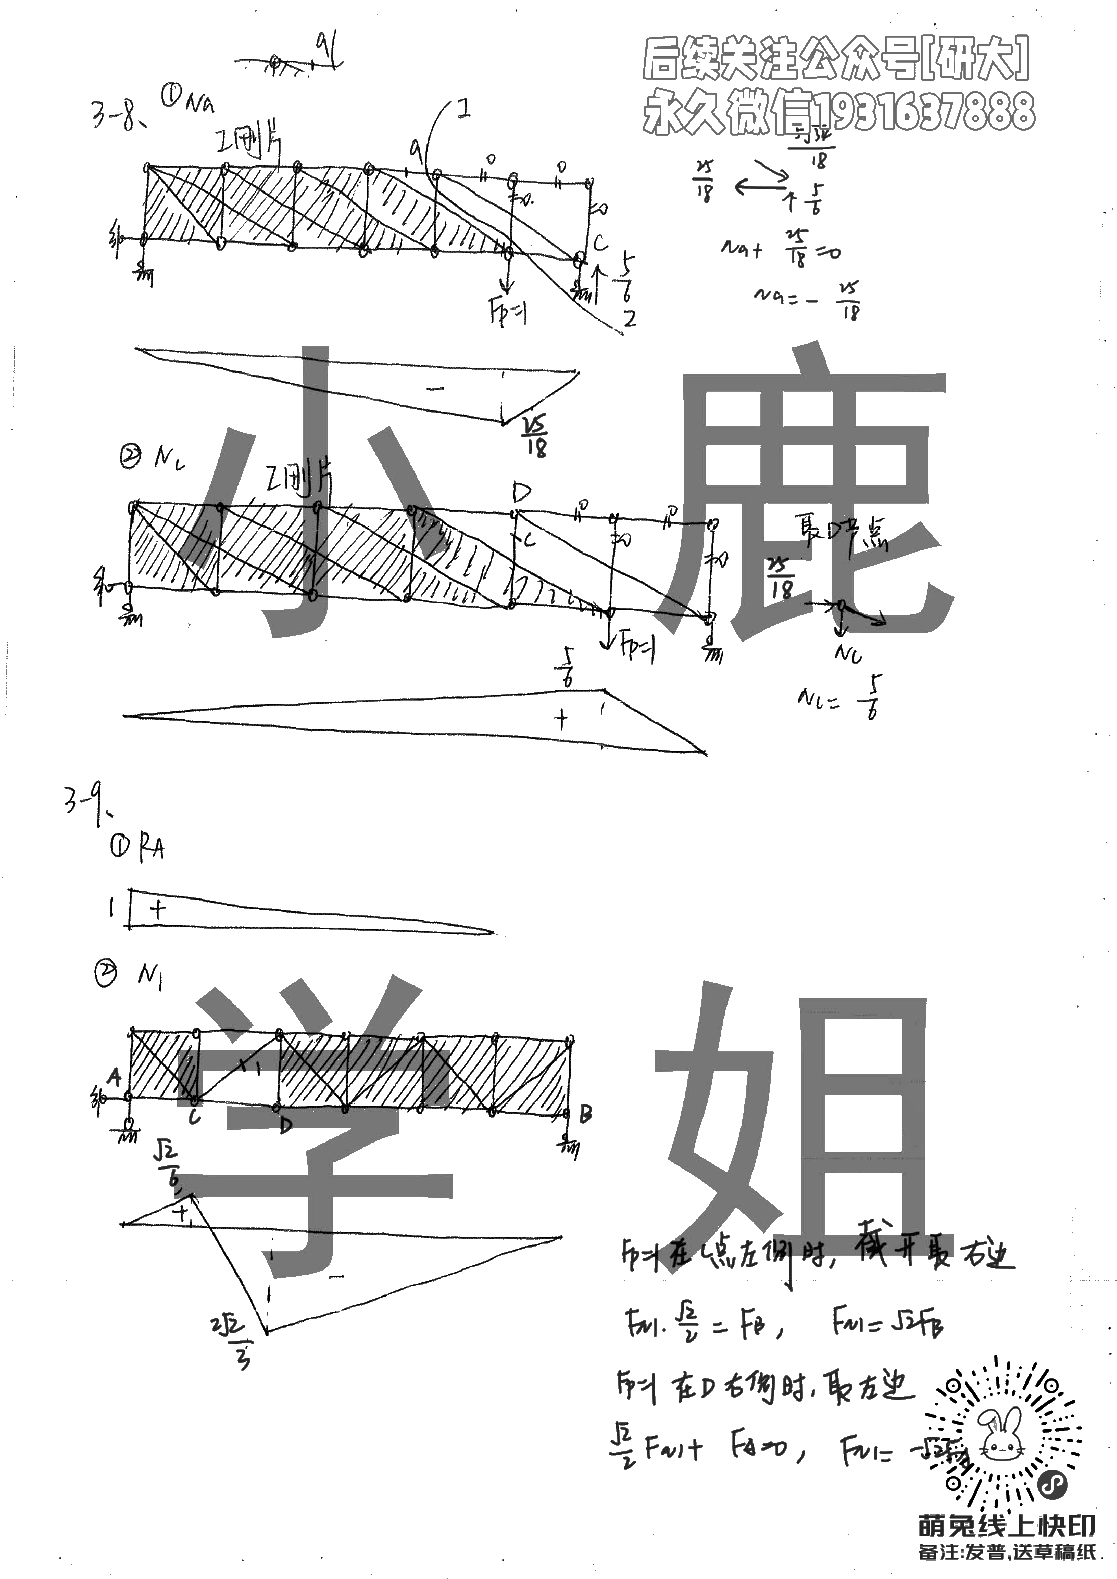
\includegraphics[width=0.96\textwidth,height=0.82\textheight,keepaspectratio]{images/c08_answer_1_p08.png}
\par\small 作业与答案（去水印版），第 8/18 页
\end{center}
\clearpage
\begin{center}
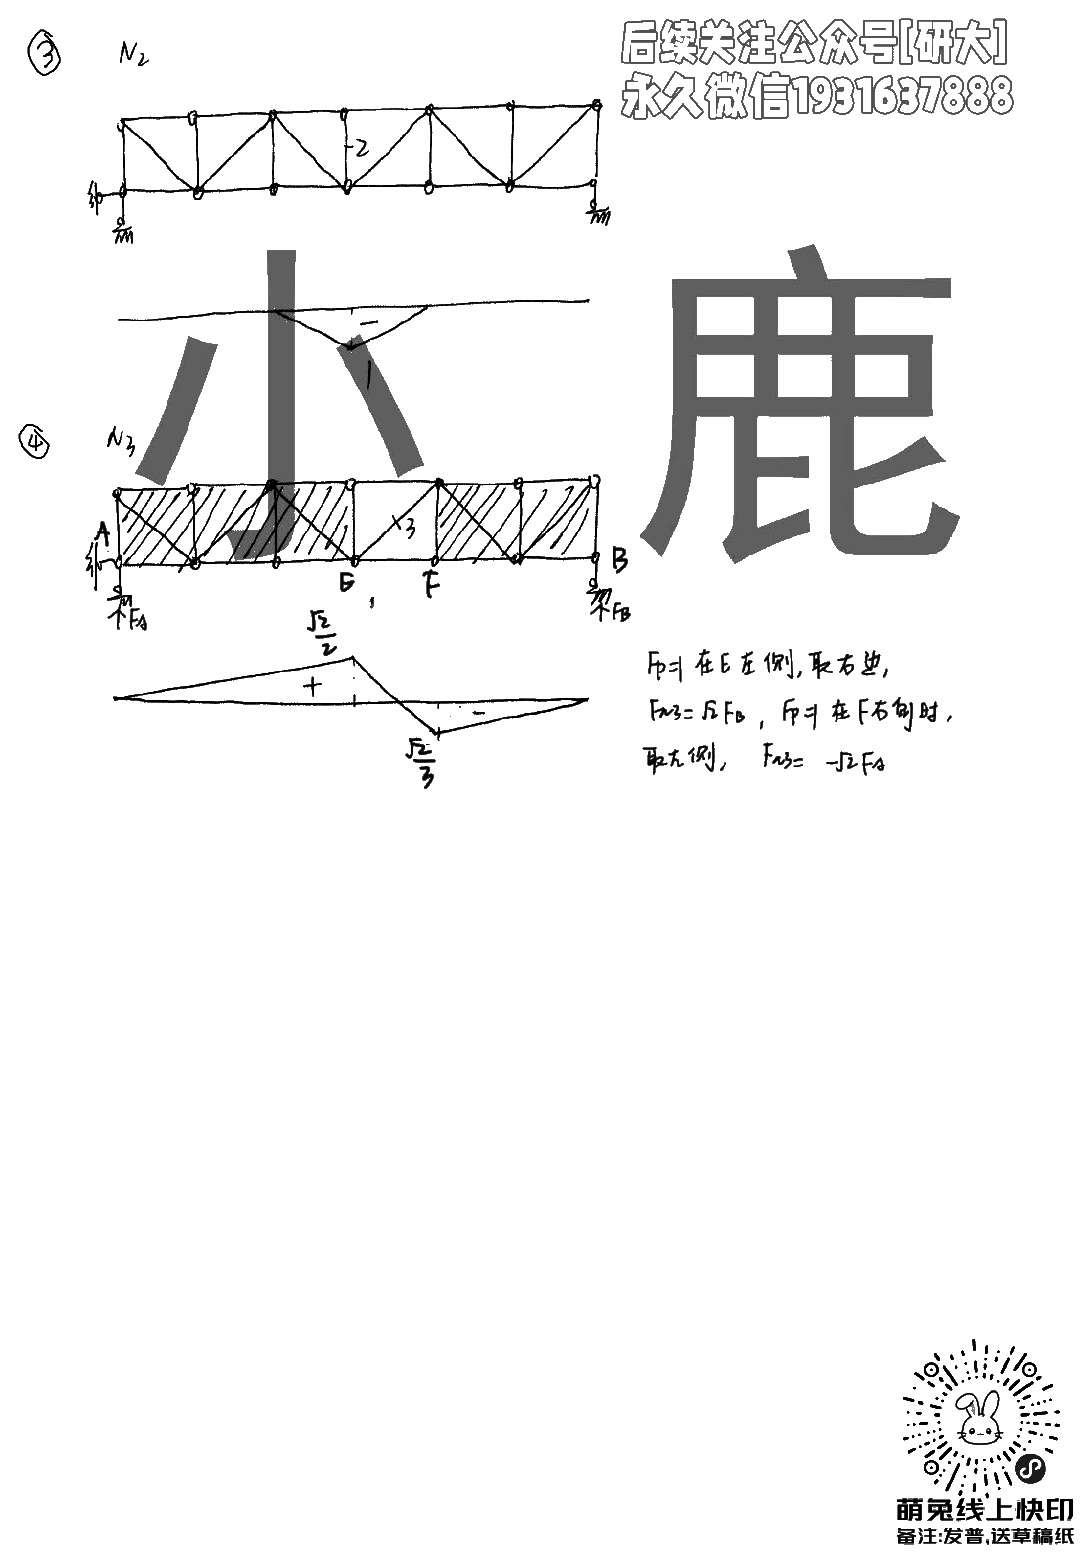
\includegraphics[width=0.96\textwidth,height=0.82\textheight,keepaspectratio]{images/c08_answer_1_p09.png}
\par\small 作业与答案（去水印版），第 9/18 页
\end{center}
\clearpage
\begin{center}
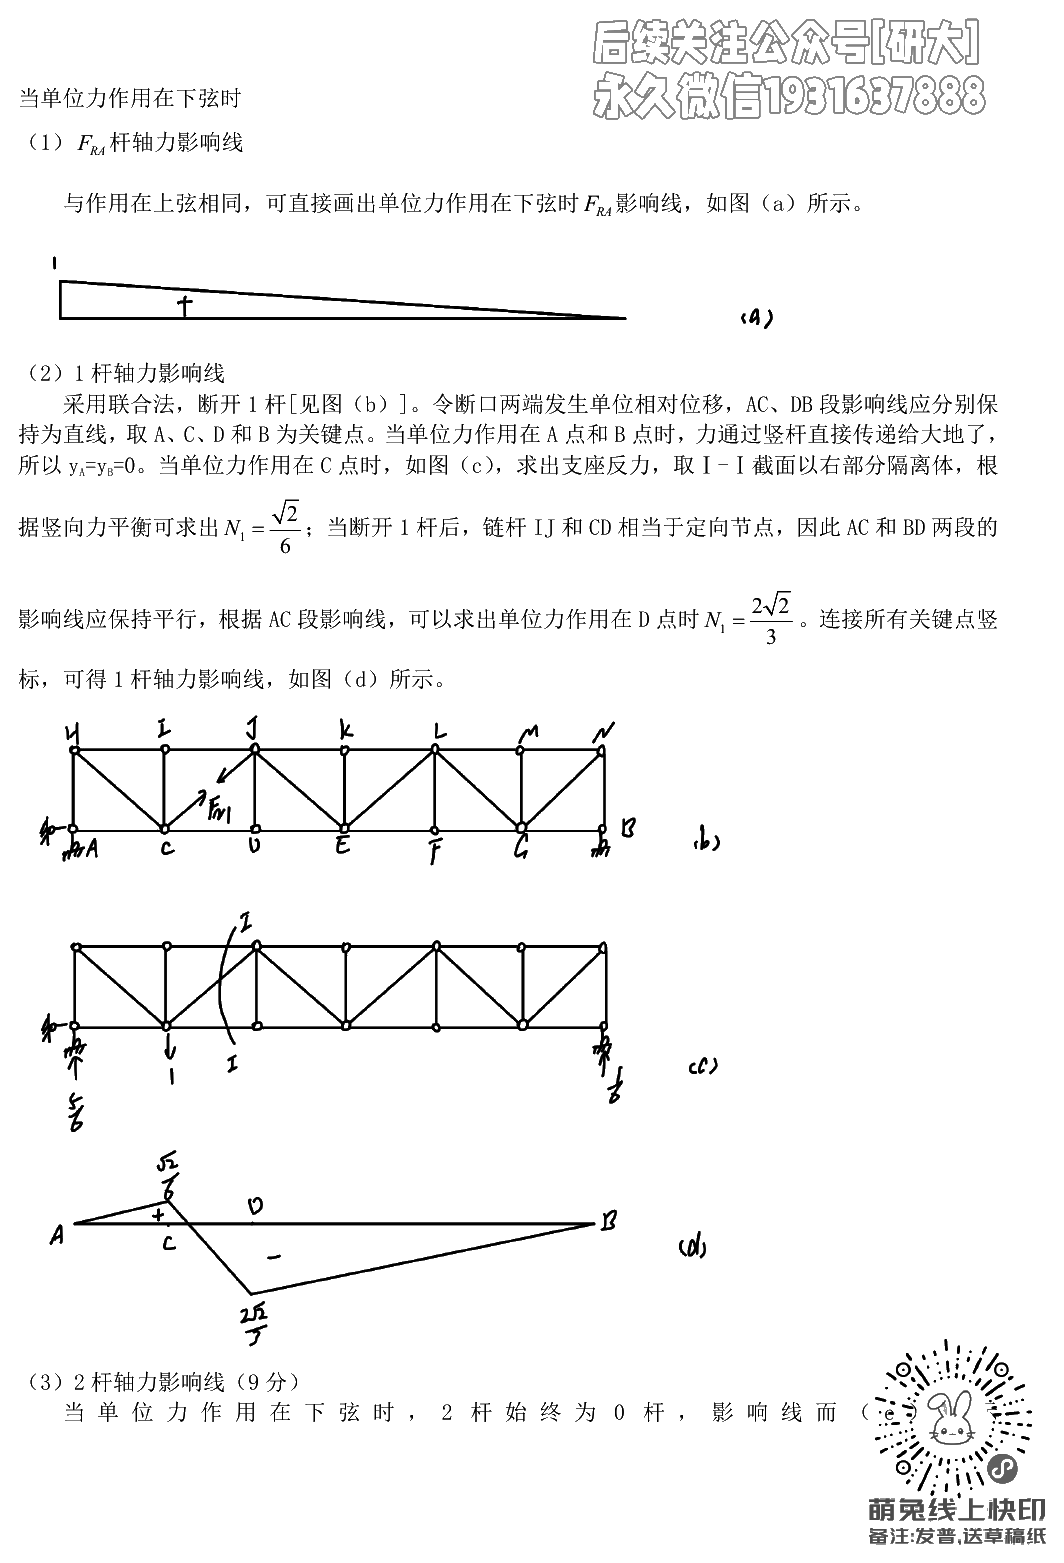
\includegraphics[width=0.96\textwidth,height=0.82\textheight,keepaspectratio]{images/c08_answer_1_p10.png}
\par\small 作业与答案（去水印版），第 10/18 页
\end{center}
\clearpage
\begin{center}
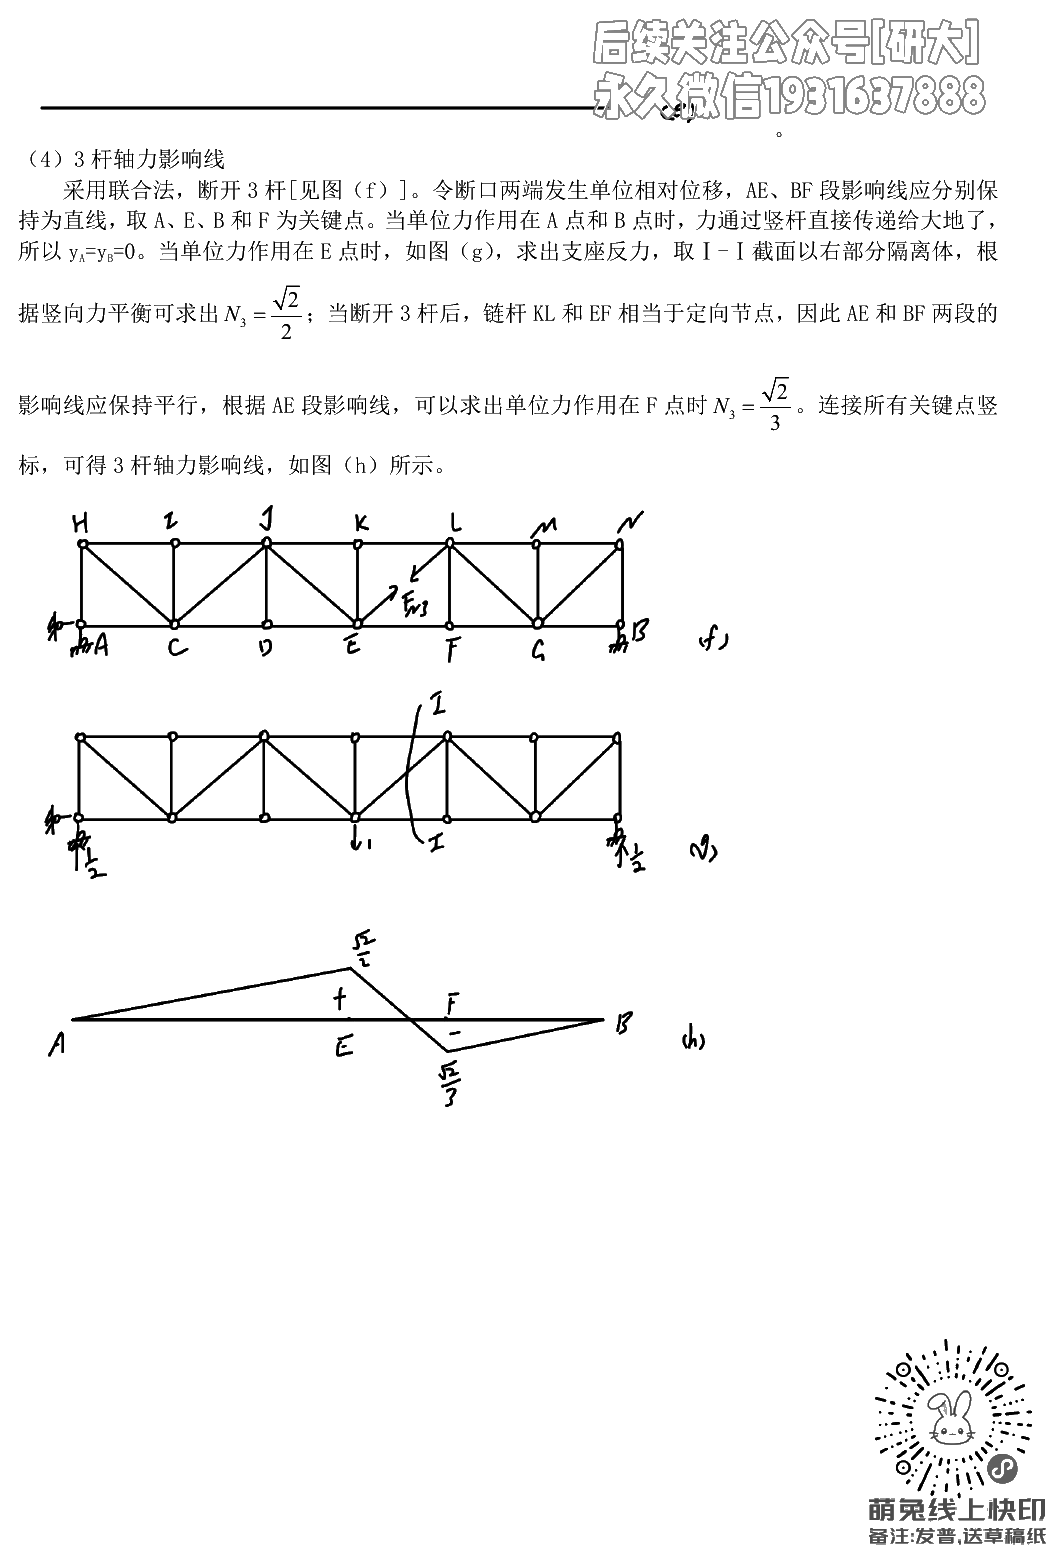
\includegraphics[width=0.96\textwidth,height=0.82\textheight,keepaspectratio]{images/c08_answer_1_p11.png}
\par\small 作业与答案（去水印版），第 11/18 页
\end{center}
\clearpage
\begin{center}
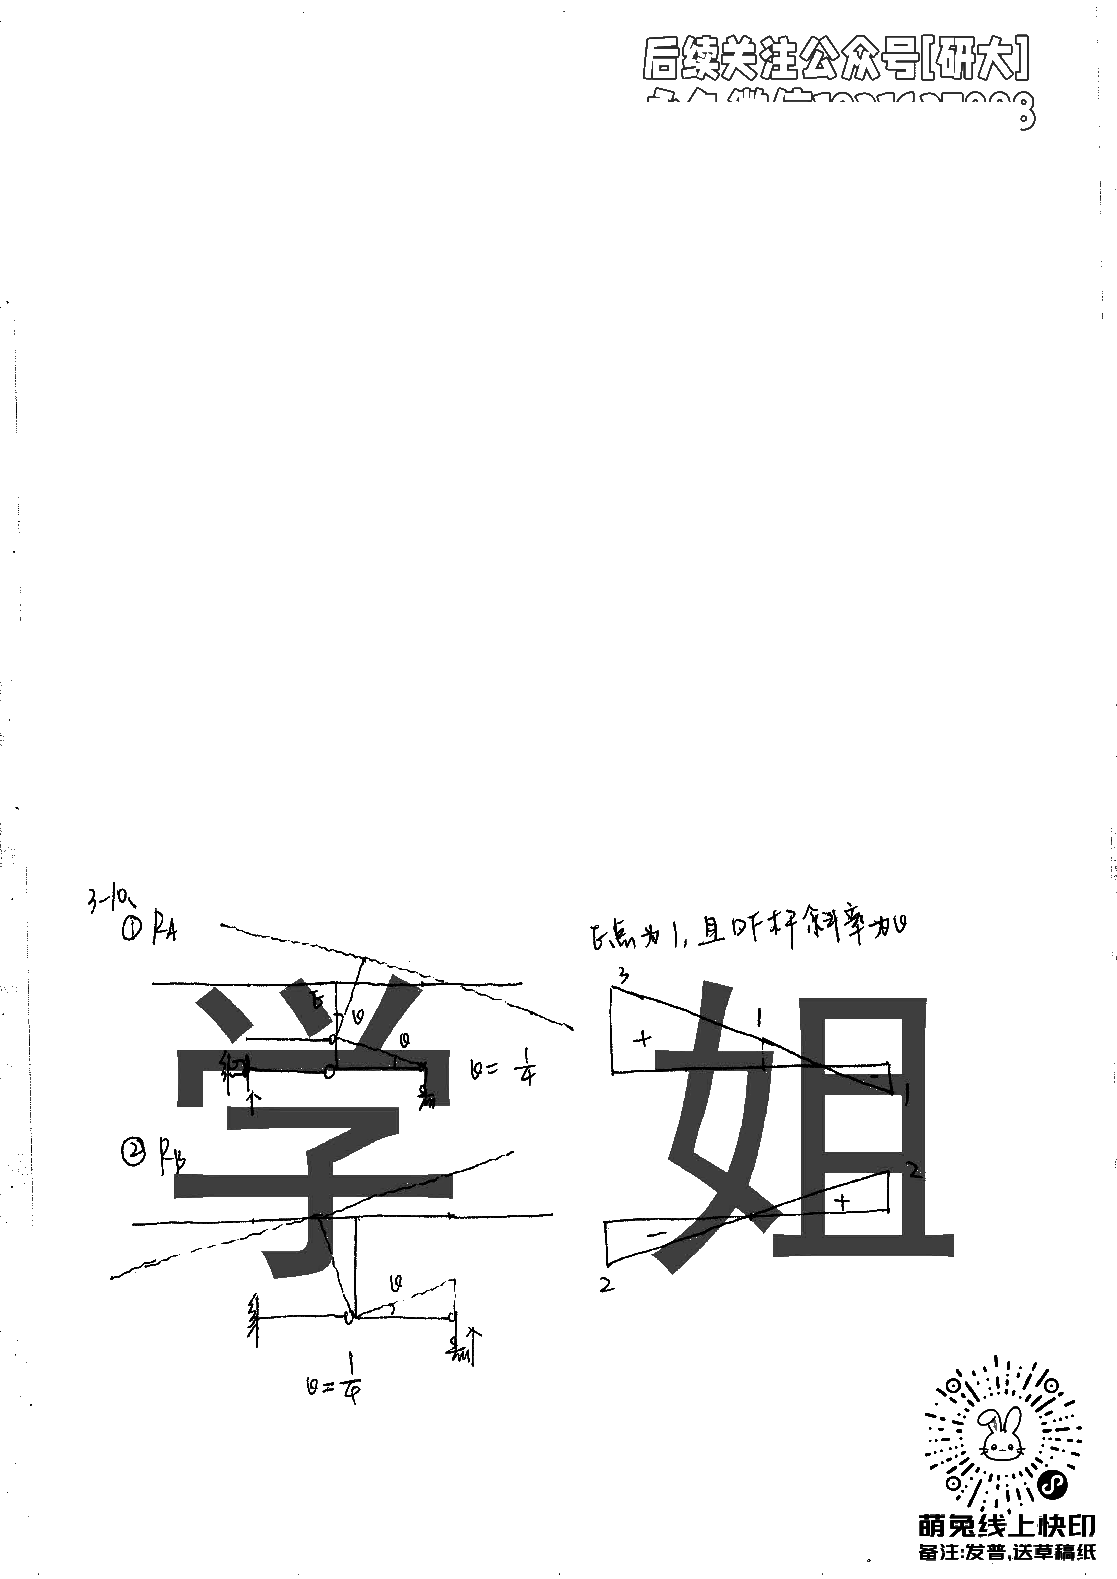
\includegraphics[width=0.96\textwidth,height=0.82\textheight,keepaspectratio]{images/c08_answer_1_p12.png}
\par\small 作业与答案（去水印版），第 12/18 页
\end{center}
\clearpage
\begin{center}
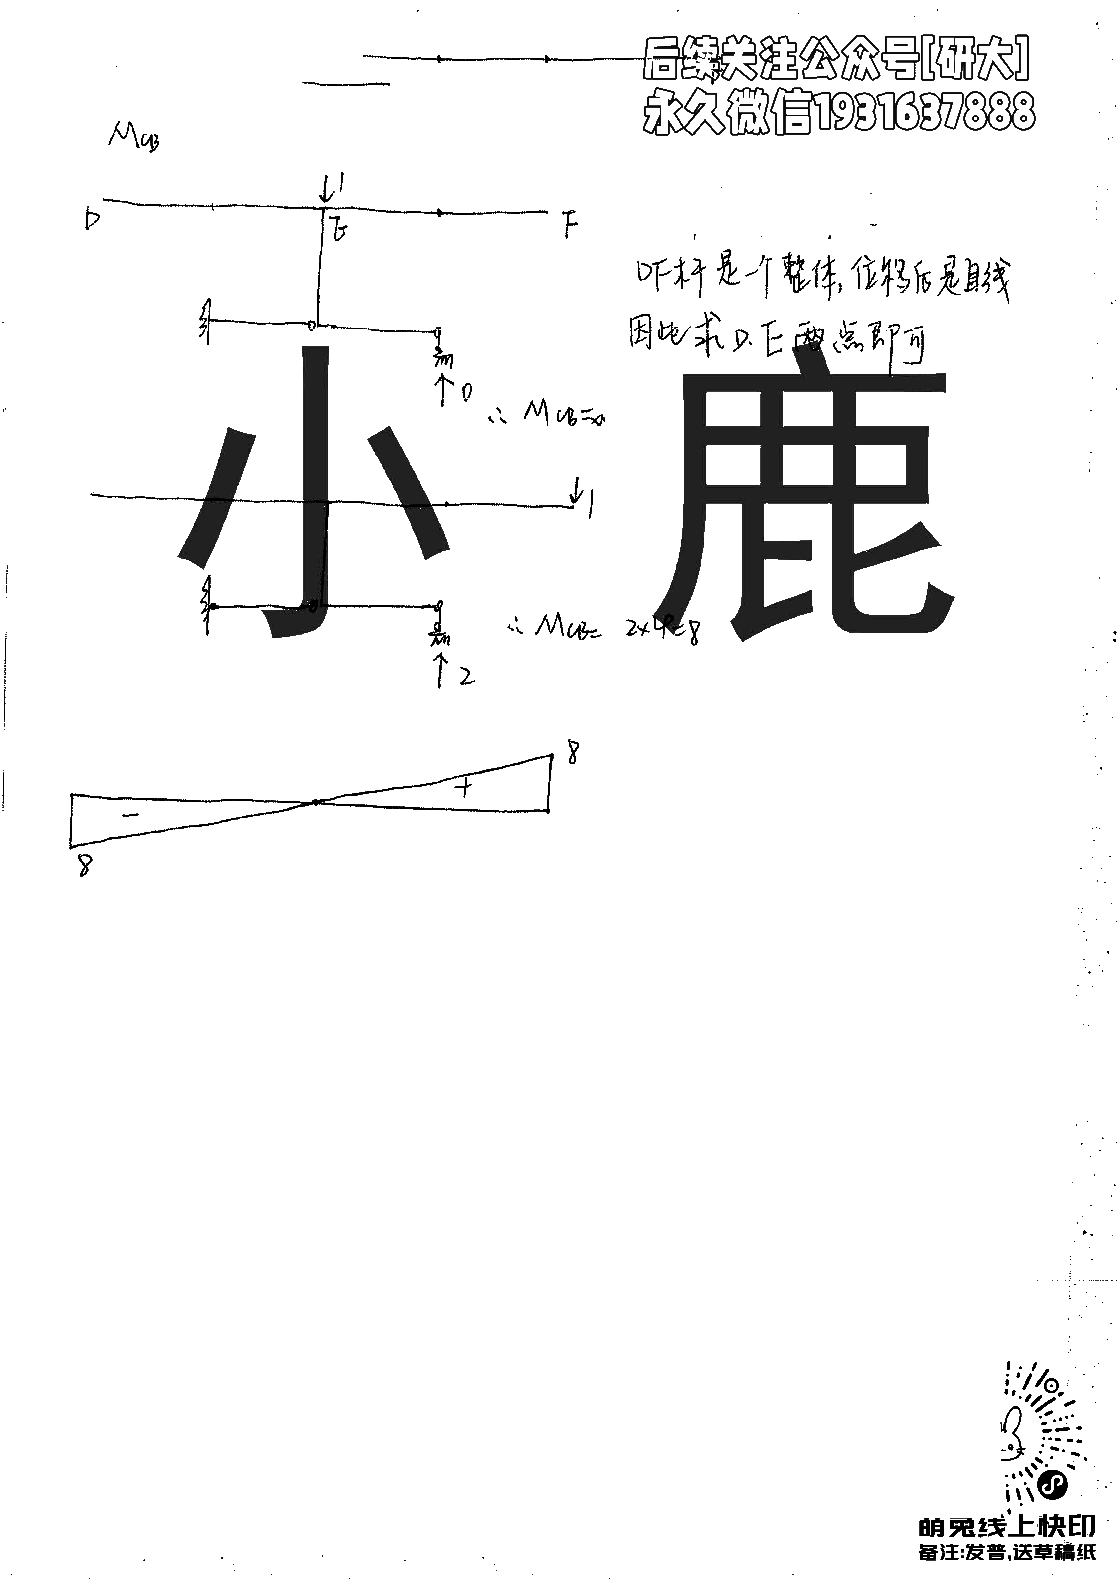
\includegraphics[width=0.96\textwidth,height=0.82\textheight,keepaspectratio]{images/c08_answer_1_p13.png}
\par\small 作业与答案（去水印版），第 13/18 页
\end{center}
\clearpage
\begin{center}
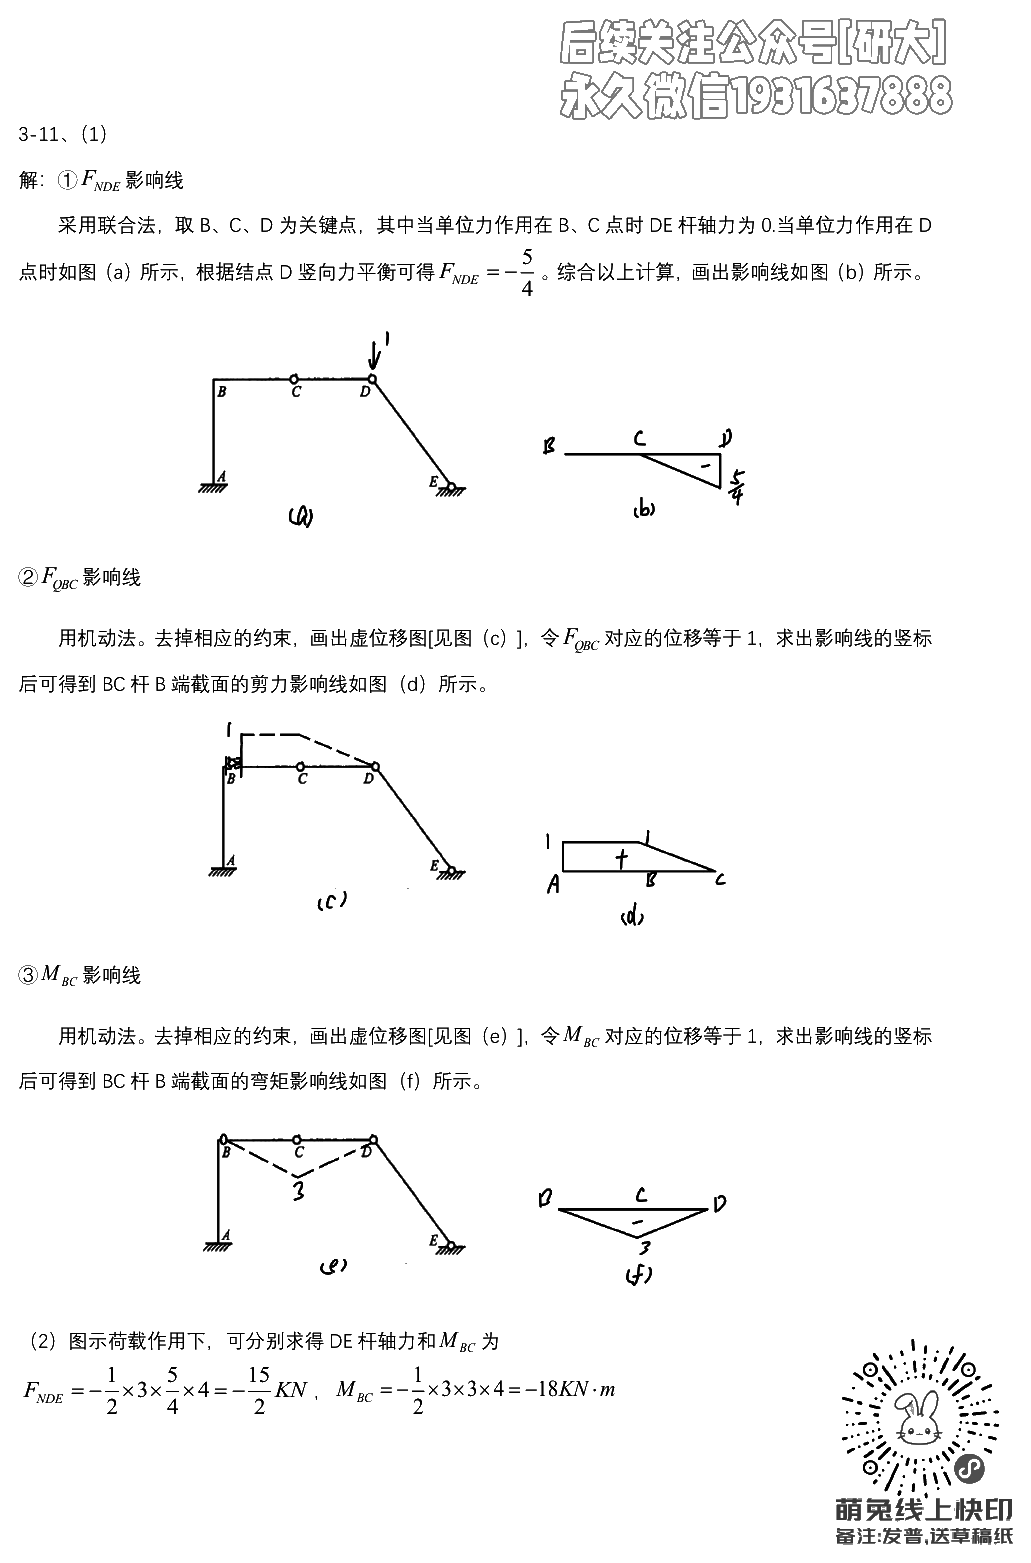
\includegraphics[width=0.96\textwidth,height=0.82\textheight,keepaspectratio]{images/c08_answer_1_p14.png}
\par\small 作业与答案（去水印版），第 14/18 页
\end{center}
\clearpage
\begin{center}
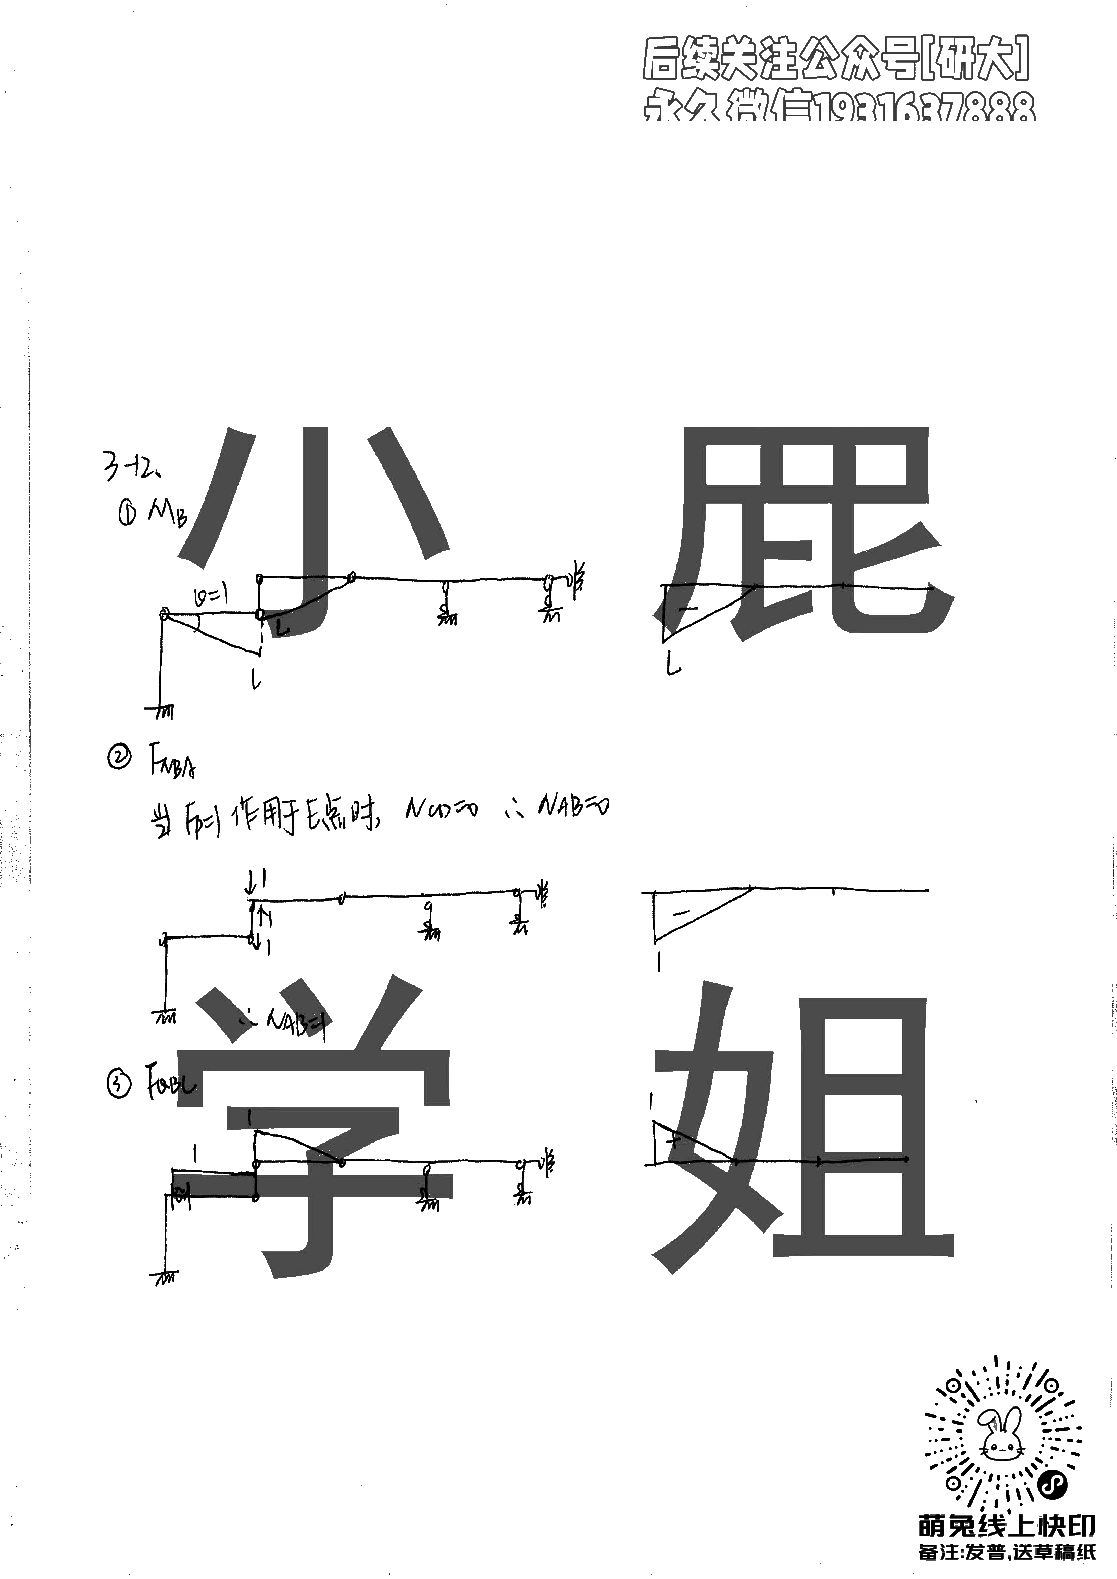
\includegraphics[width=0.96\textwidth,height=0.82\textheight,keepaspectratio]{images/c08_answer_1_p15.png}
\par\small 作业与答案（去水印版），第 15/18 页
\end{center}
\clearpage
\begin{center}
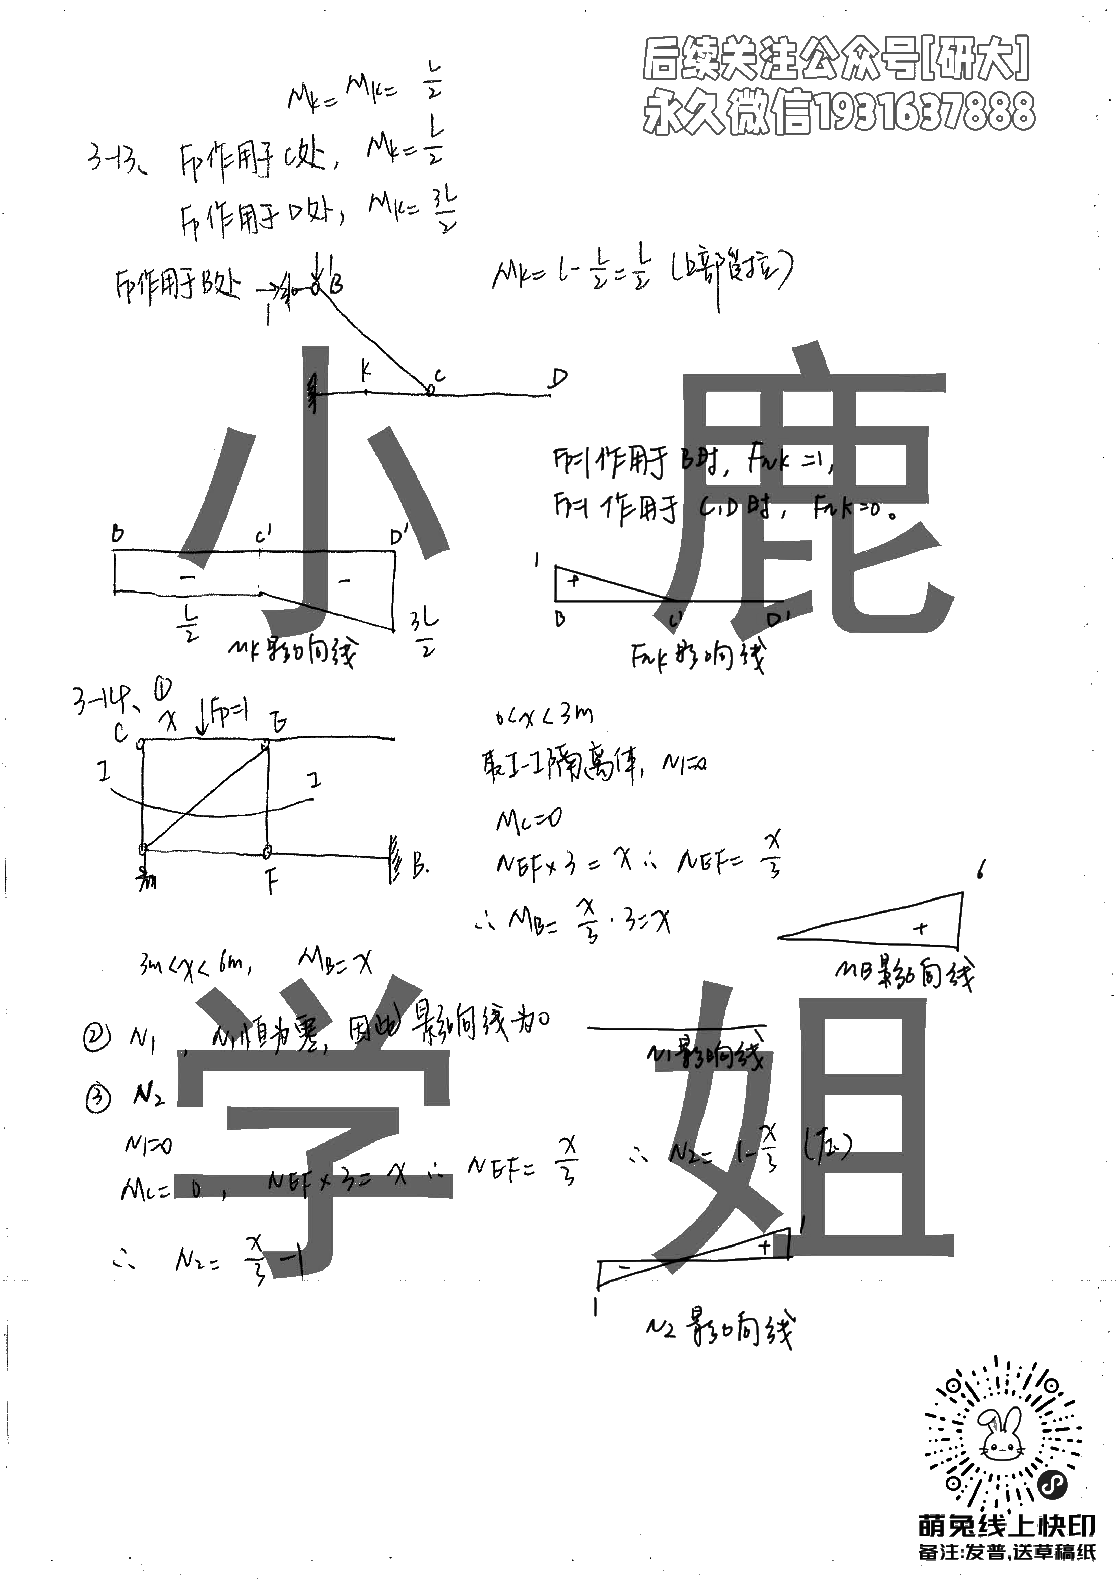
\includegraphics[width=0.96\textwidth,height=0.82\textheight,keepaspectratio]{images/c08_answer_1_p16.png}
\par\small 作业与答案（去水印版），第 16/18 页
\end{center}
\clearpage
\begin{center}
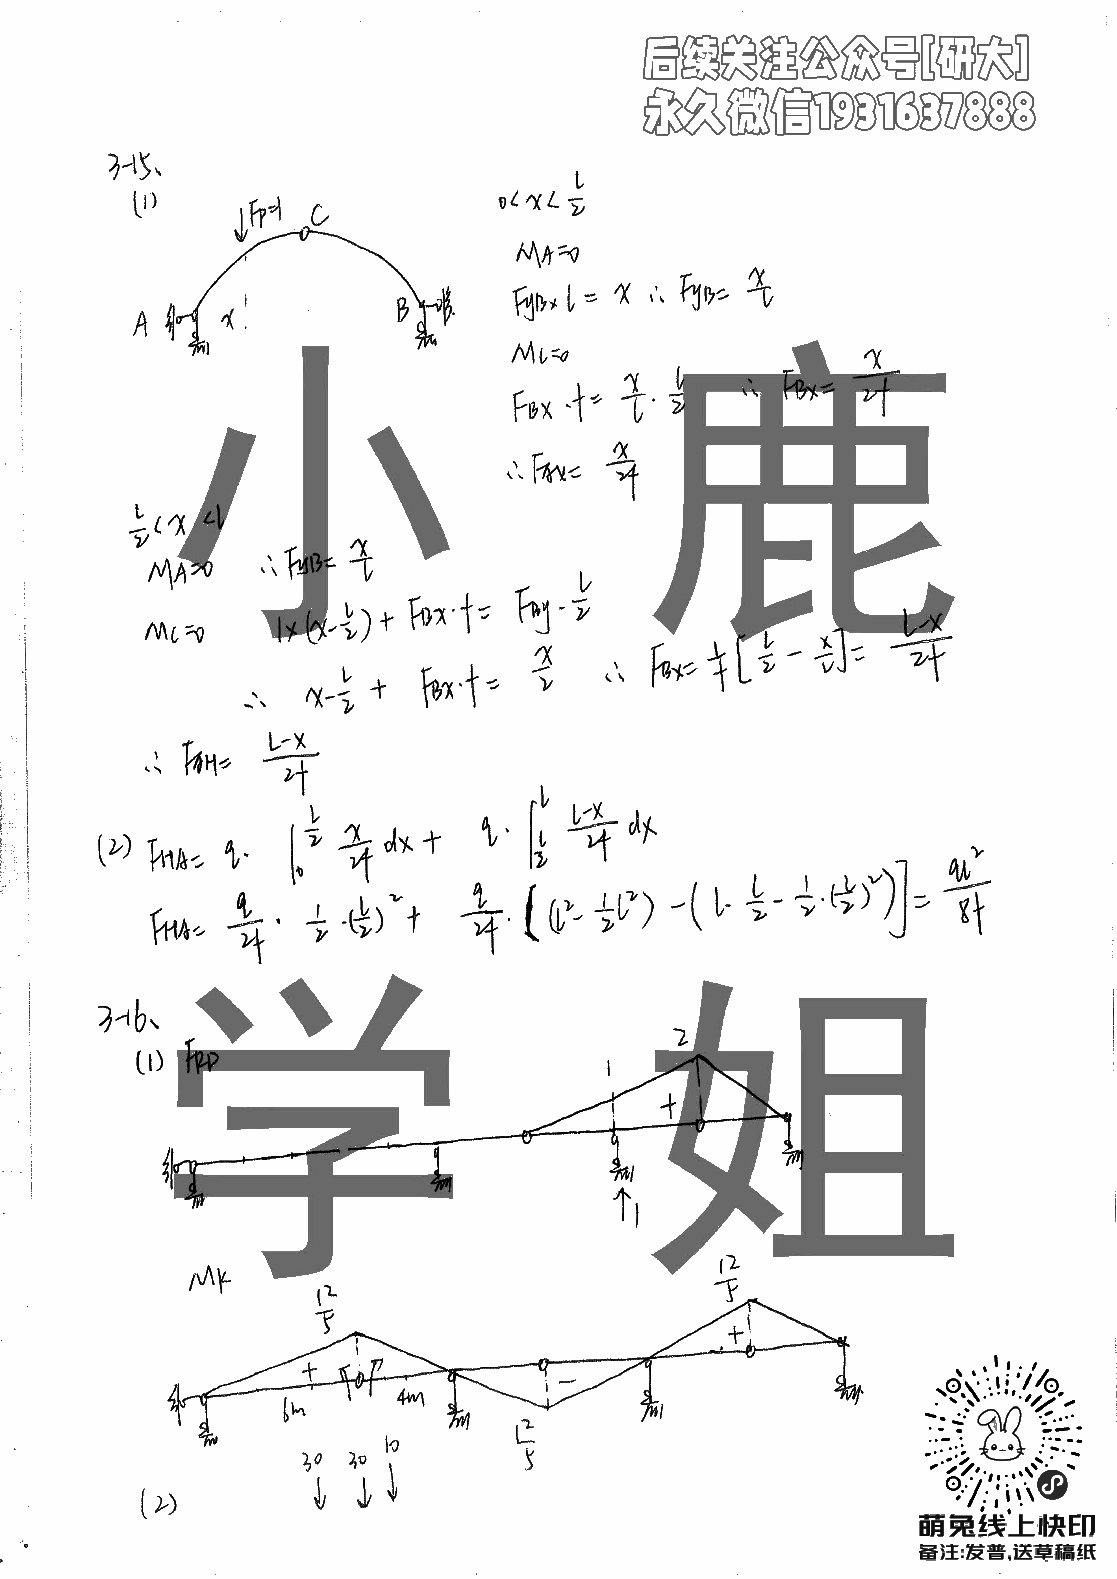
\includegraphics[width=0.96\textwidth,height=0.82\textheight,keepaspectratio]{images/c08_answer_1_p17.png}
\par\small 作业与答案（去水印版），第 17/18 页
\end{center}
\clearpage
\begin{center}
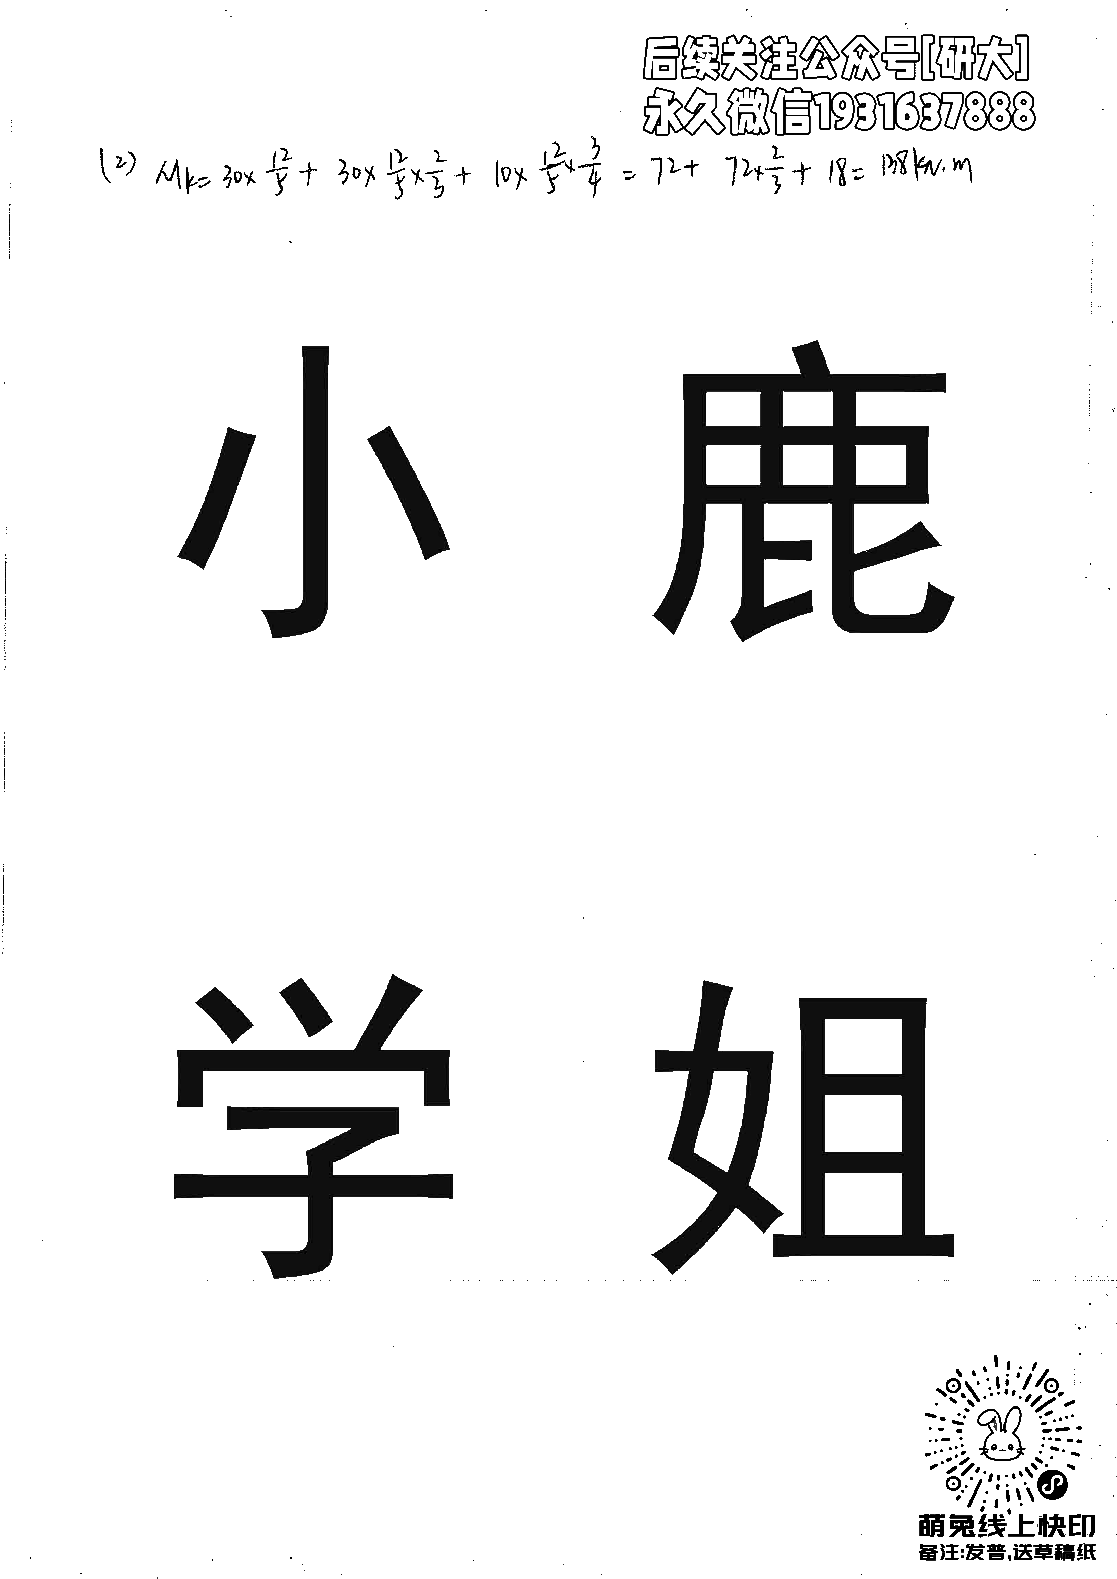
\includegraphics[width=0.96\textwidth,height=0.82\textheight,keepaspectratio]{images/c08_answer_1_p18.png}
\par\small 作业与答案（去水印版），第 18/18 页
\end{center}
\clearpage
\section{讲解笔记（去水印版）}
\begin{center}
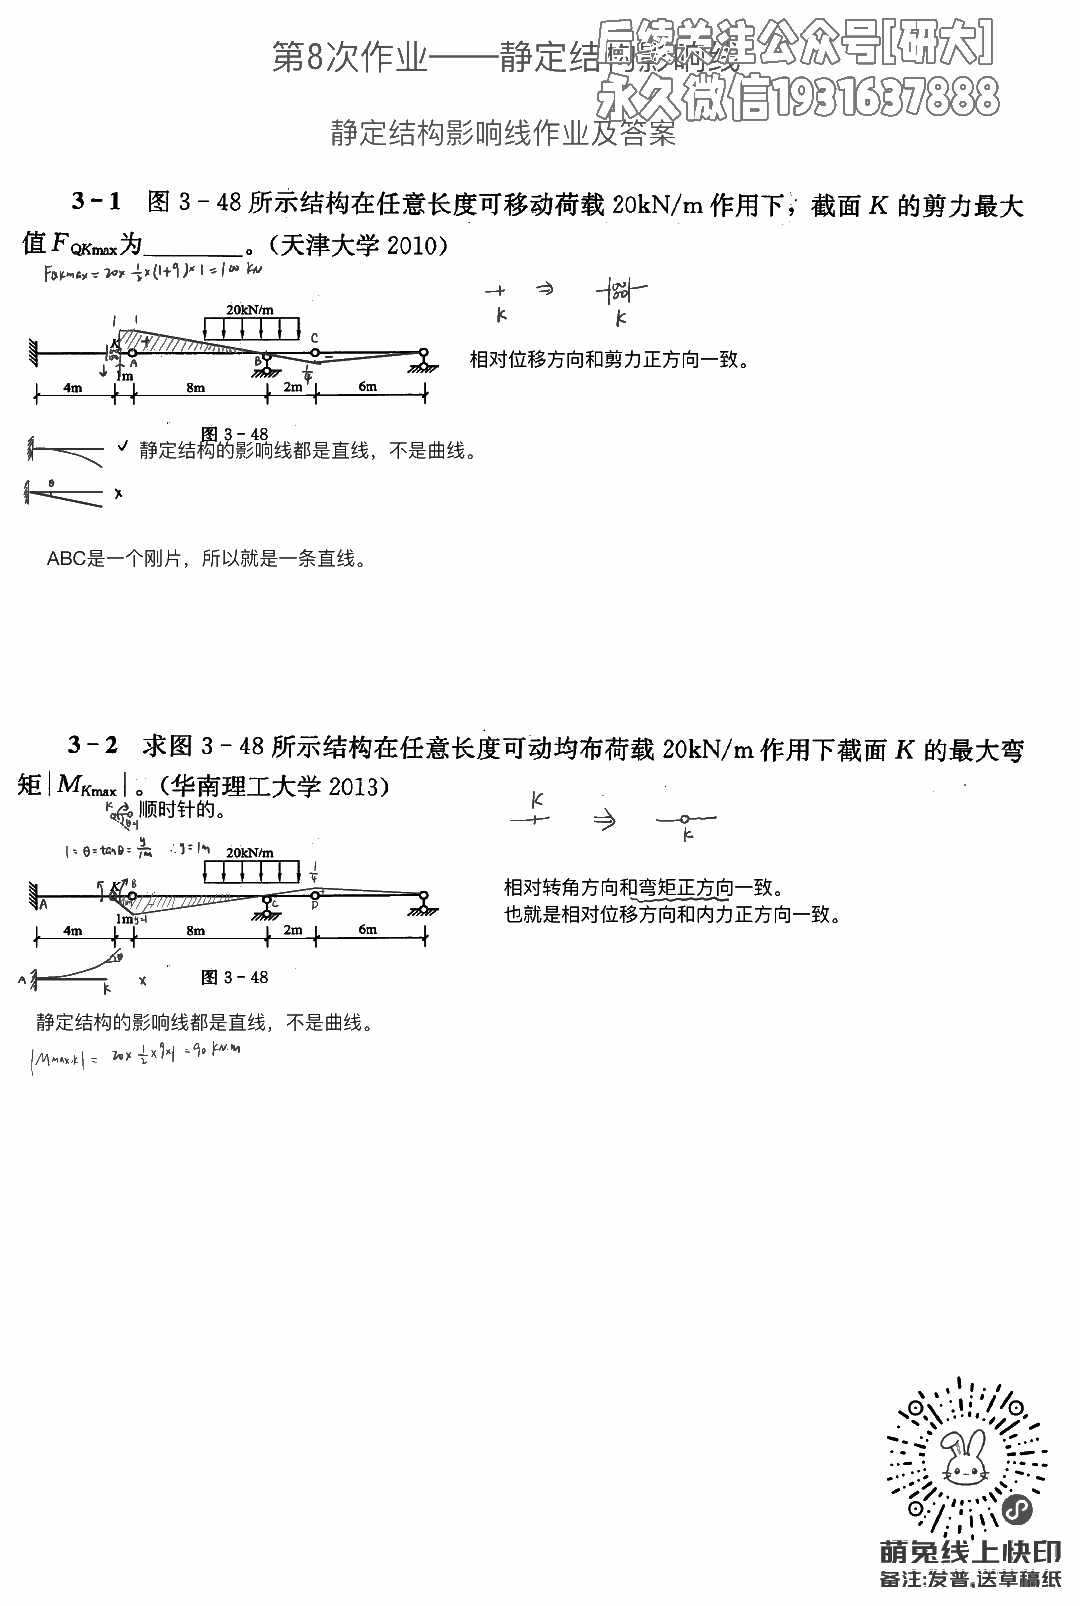
\includegraphics[width=0.96\textwidth,height=0.82\textheight,keepaspectratio]{images/c08_note_p01.png}
\par\small 讲解笔记（去水印版），第 1/11 页
\end{center}
\clearpage
\begin{center}
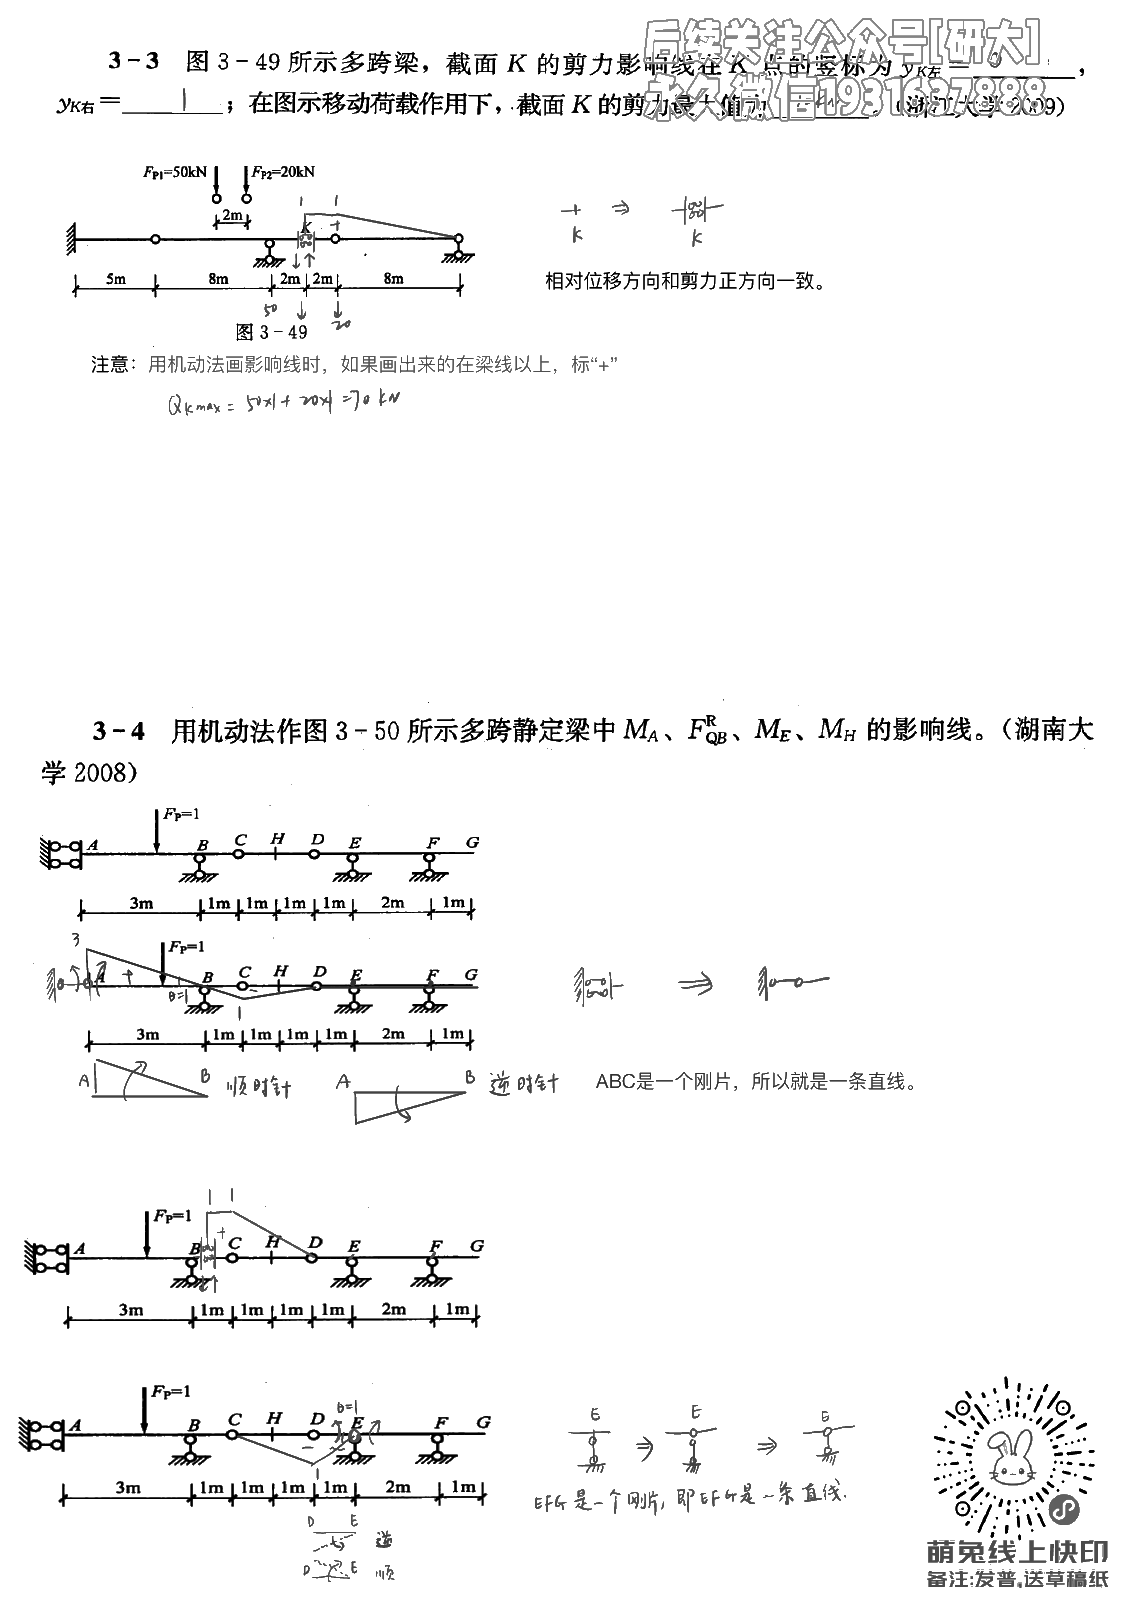
\includegraphics[width=0.96\textwidth,height=0.82\textheight,keepaspectratio]{images/c08_note_p02.png}
\par\small 讲解笔记（去水印版），第 2/11 页
\end{center}
\clearpage
\begin{center}
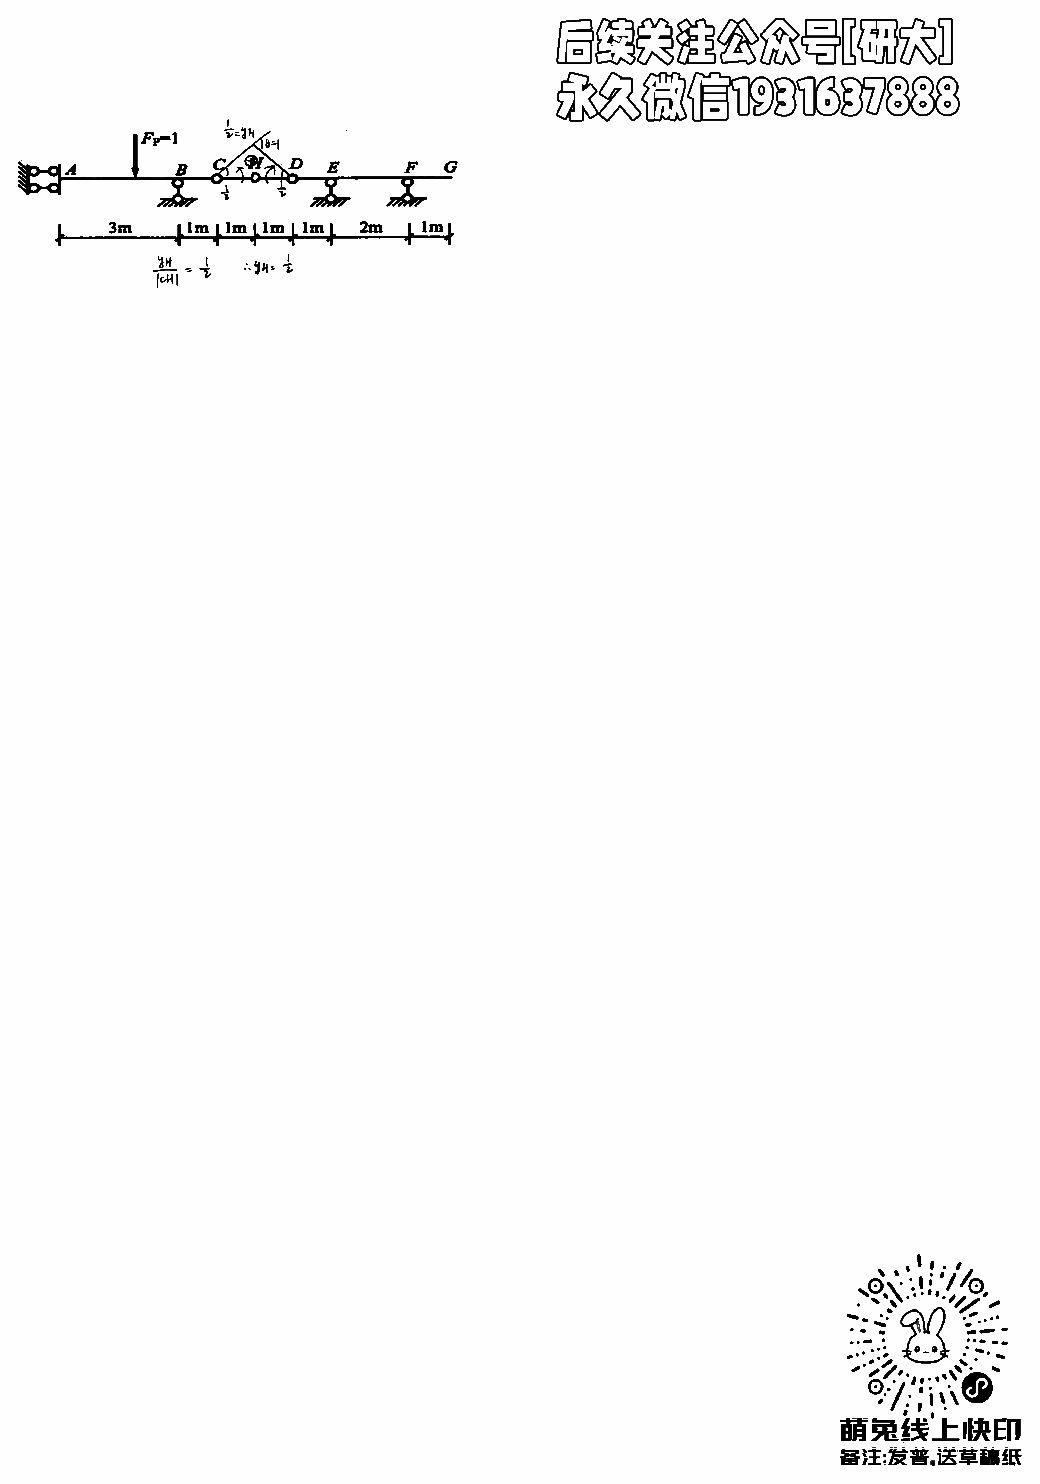
\includegraphics[width=0.96\textwidth,height=0.82\textheight,keepaspectratio]{images/c08_note_p03.png}
\par\small 讲解笔记（去水印版），第 3/11 页
\end{center}
\clearpage
\begin{center}
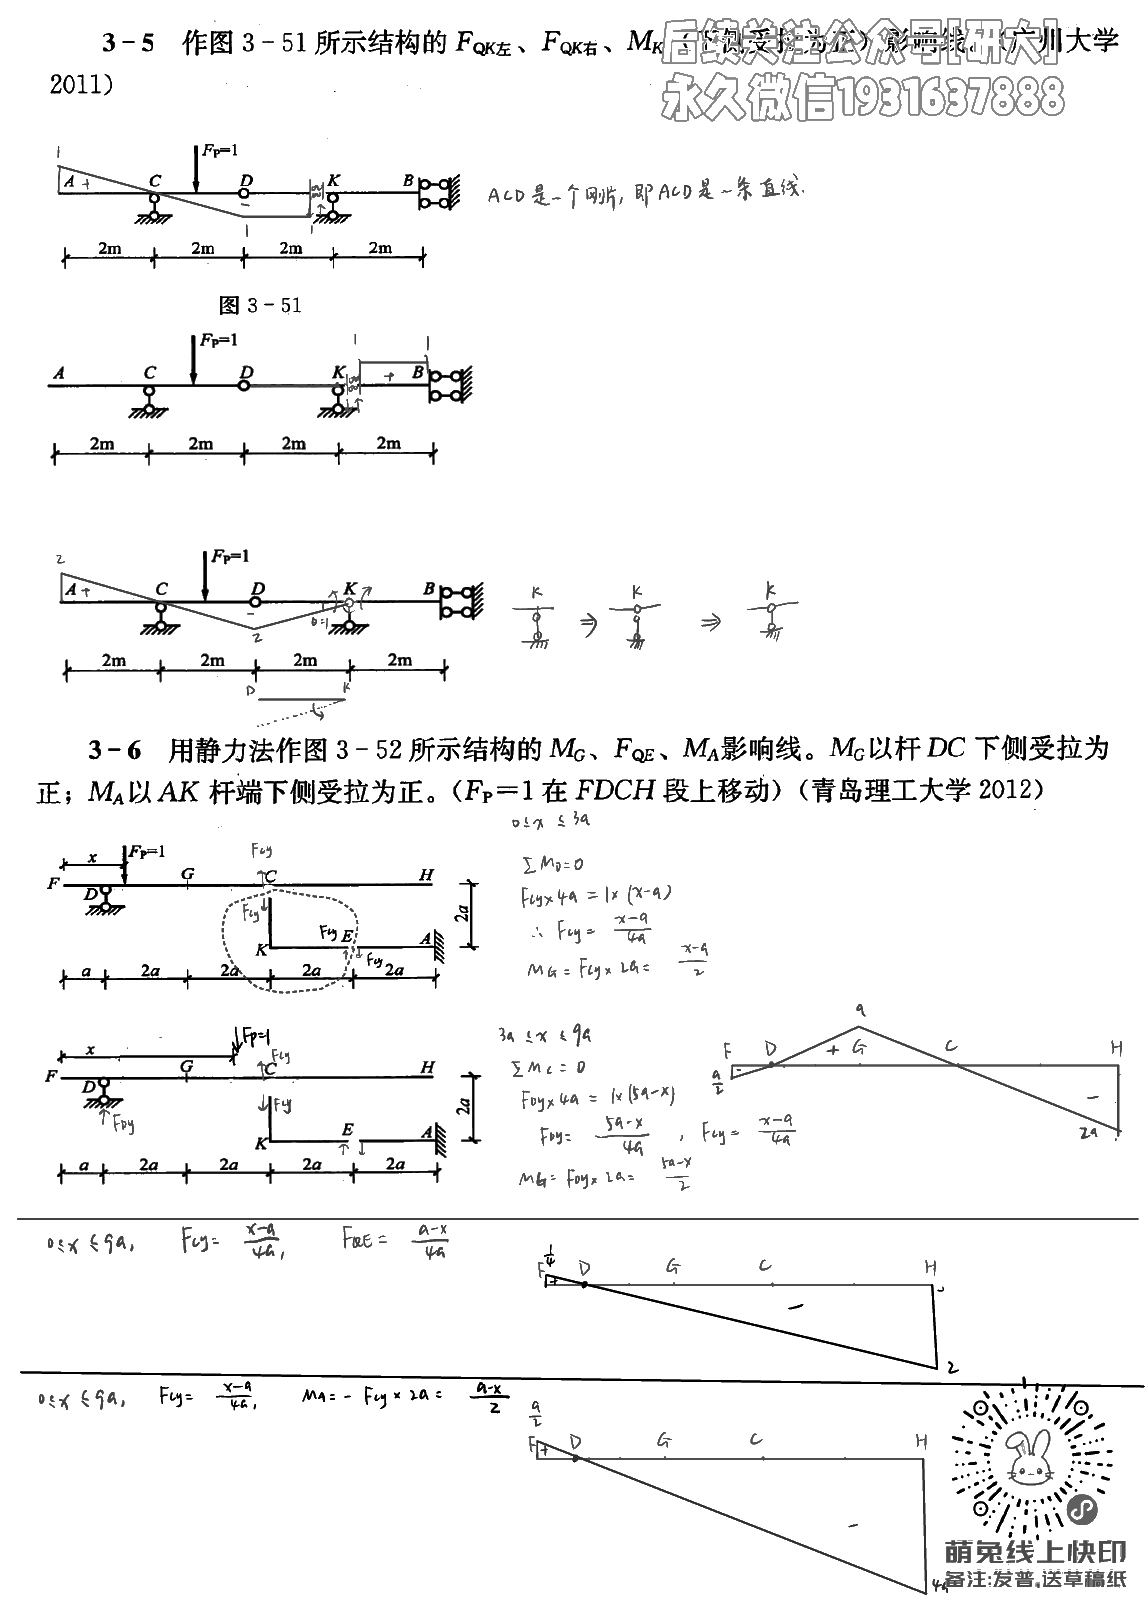
\includegraphics[width=0.96\textwidth,height=0.82\textheight,keepaspectratio]{images/c08_note_p04.png}
\par\small 讲解笔记（去水印版），第 4/11 页
\end{center}
\clearpage
\begin{center}
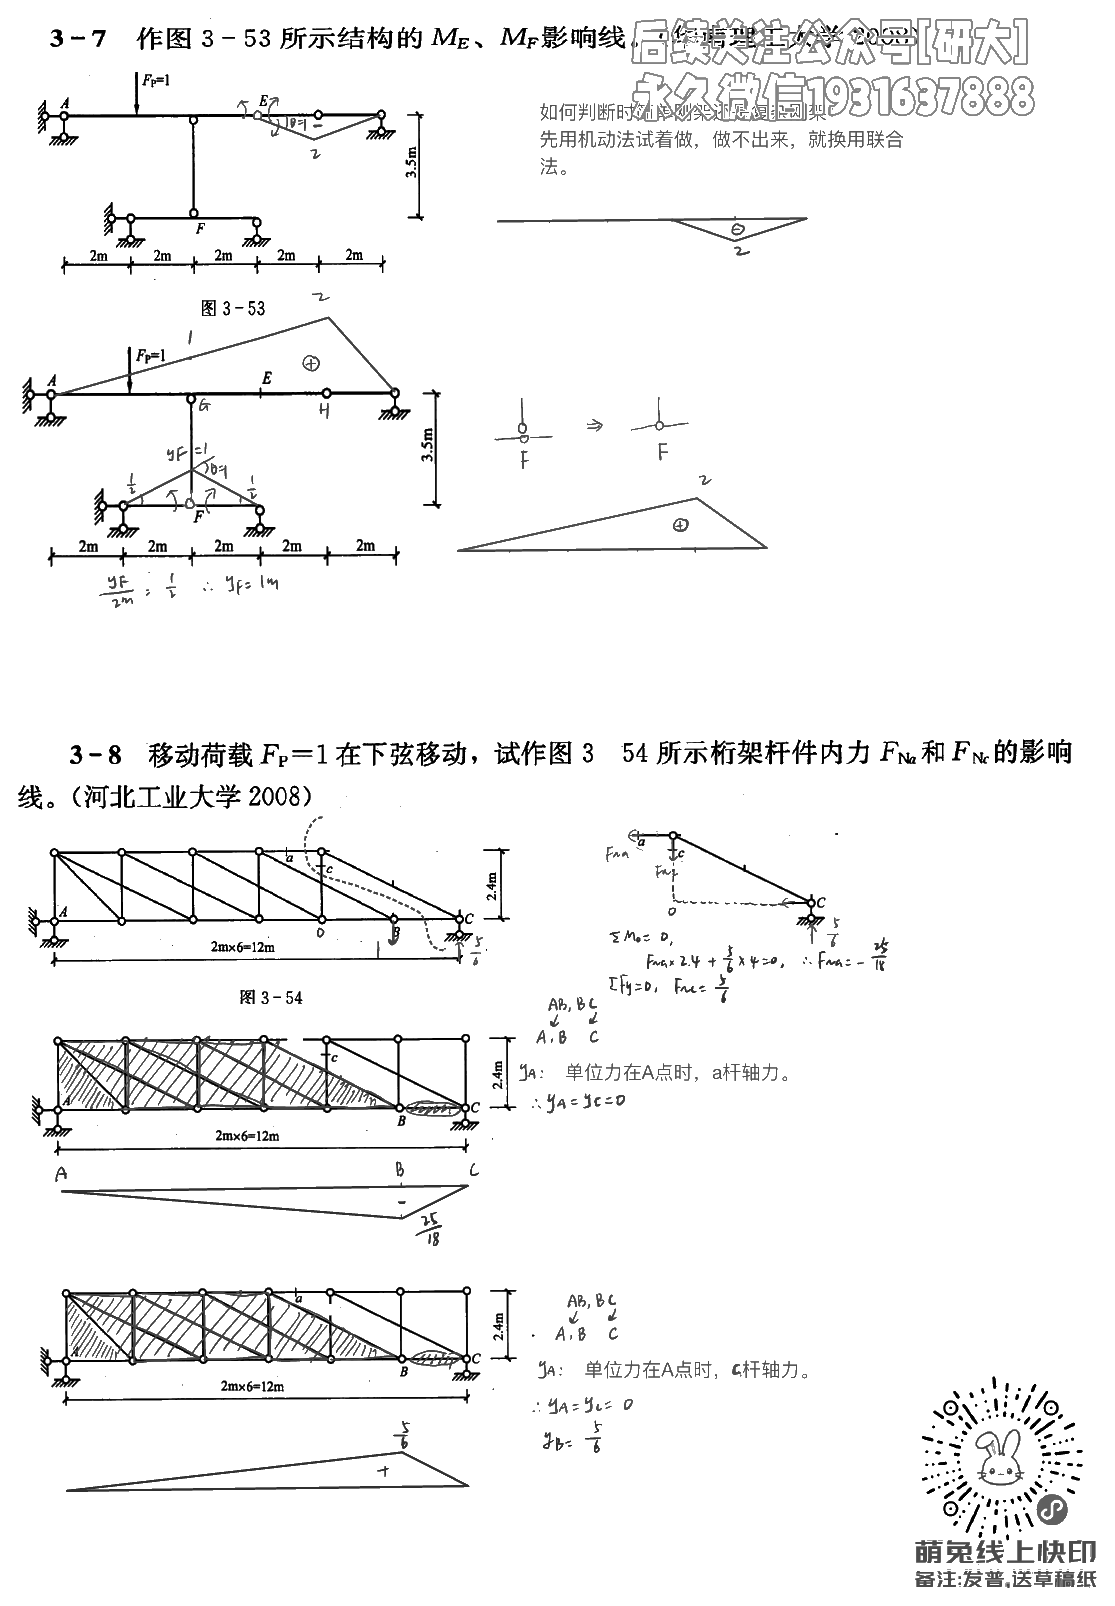
\includegraphics[width=0.96\textwidth,height=0.82\textheight,keepaspectratio]{images/c08_note_p05.png}
\par\small 讲解笔记（去水印版），第 5/11 页
\end{center}
\clearpage
\begin{center}
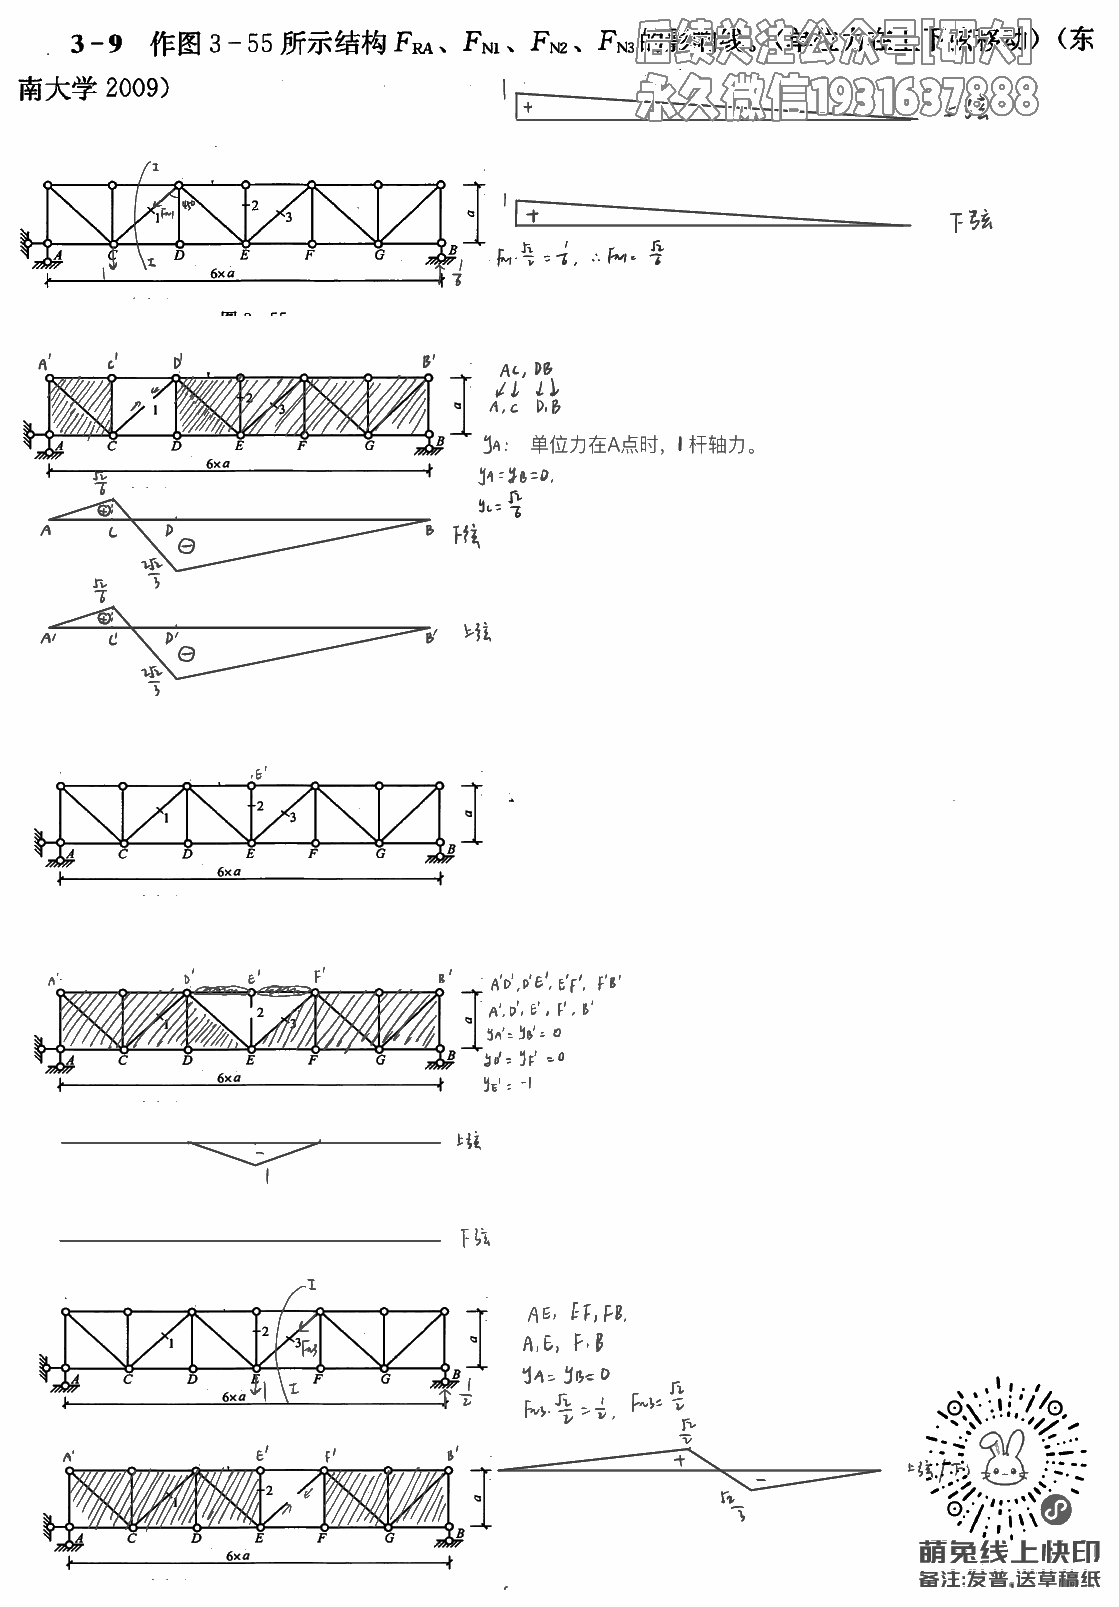
\includegraphics[width=0.96\textwidth,height=0.82\textheight,keepaspectratio]{images/c08_note_p06.png}
\par\small 讲解笔记（去水印版），第 6/11 页
\end{center}
\clearpage
\begin{center}
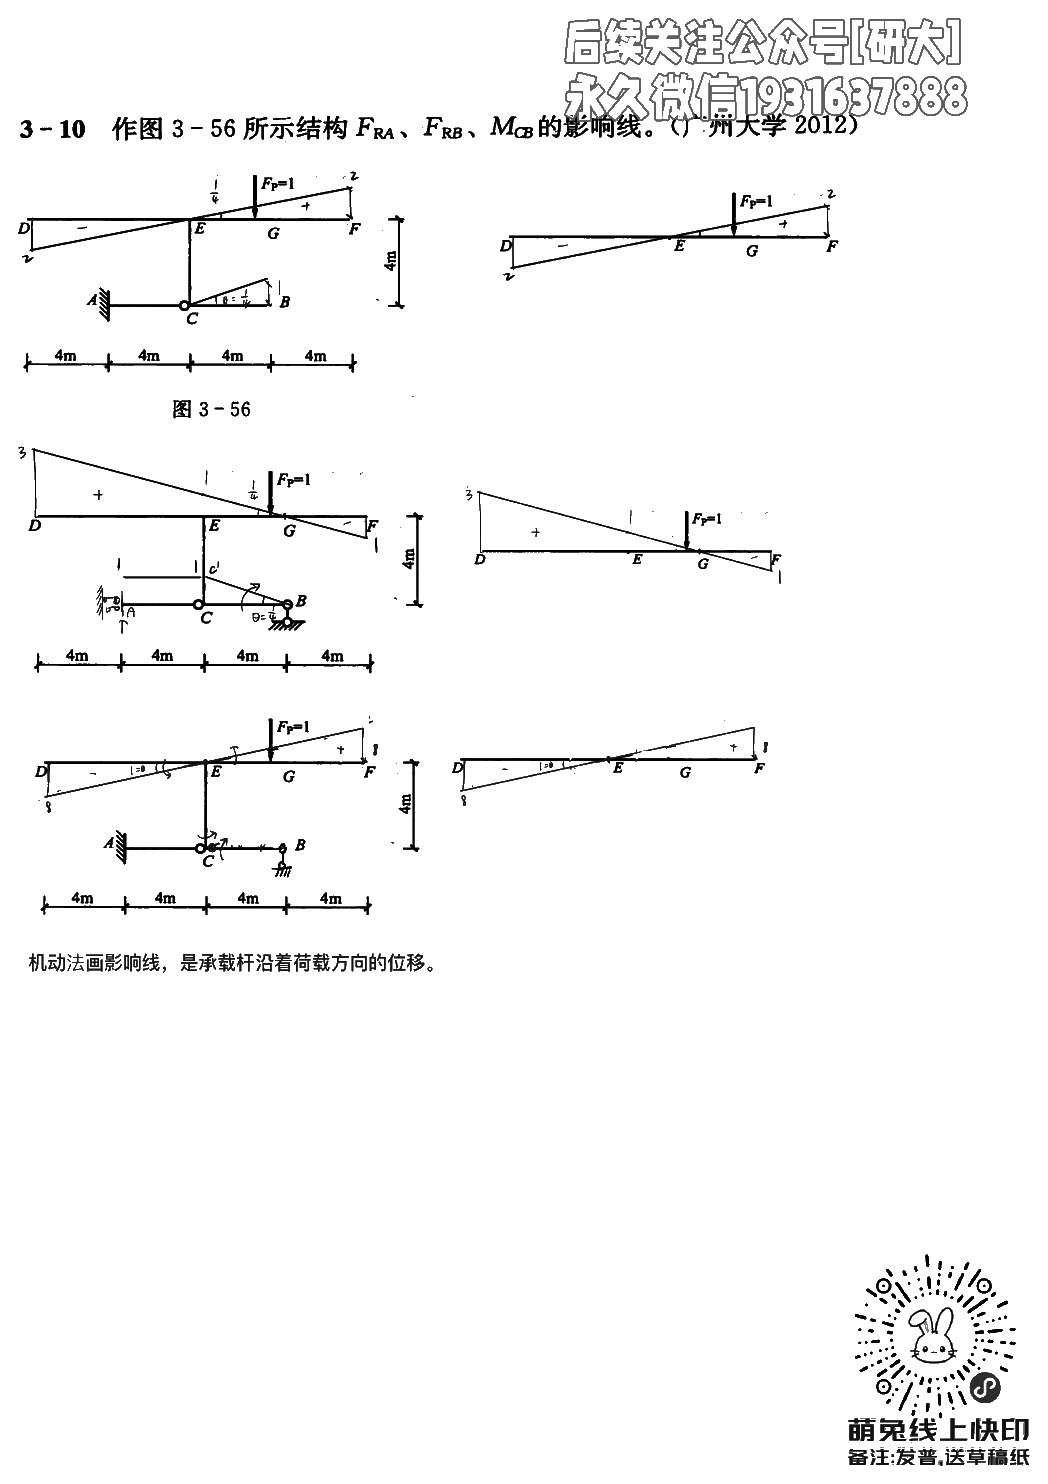
\includegraphics[width=0.96\textwidth,height=0.82\textheight,keepaspectratio]{images/c08_note_p07.png}
\par\small 讲解笔记（去水印版），第 7/11 页
\end{center}
\clearpage
\begin{center}
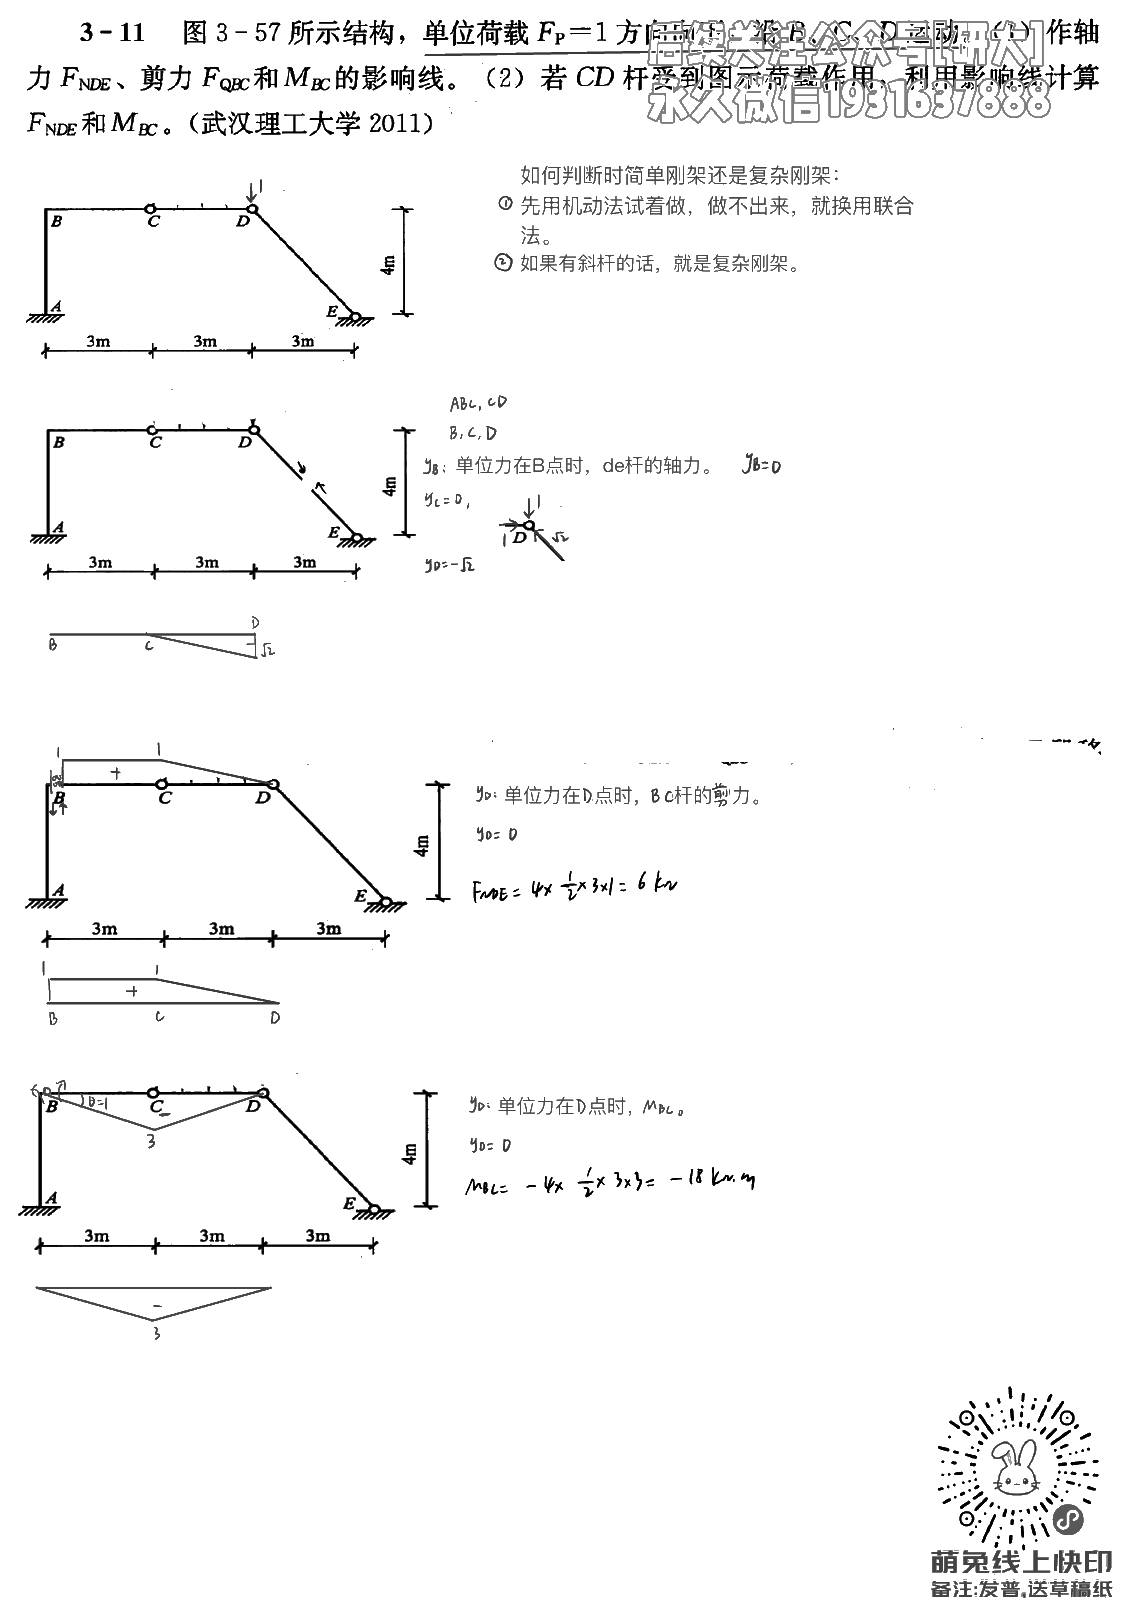
\includegraphics[width=0.96\textwidth,height=0.82\textheight,keepaspectratio]{images/c08_note_p08.png}
\par\small 讲解笔记（去水印版），第 8/11 页
\end{center}
\clearpage
\begin{center}
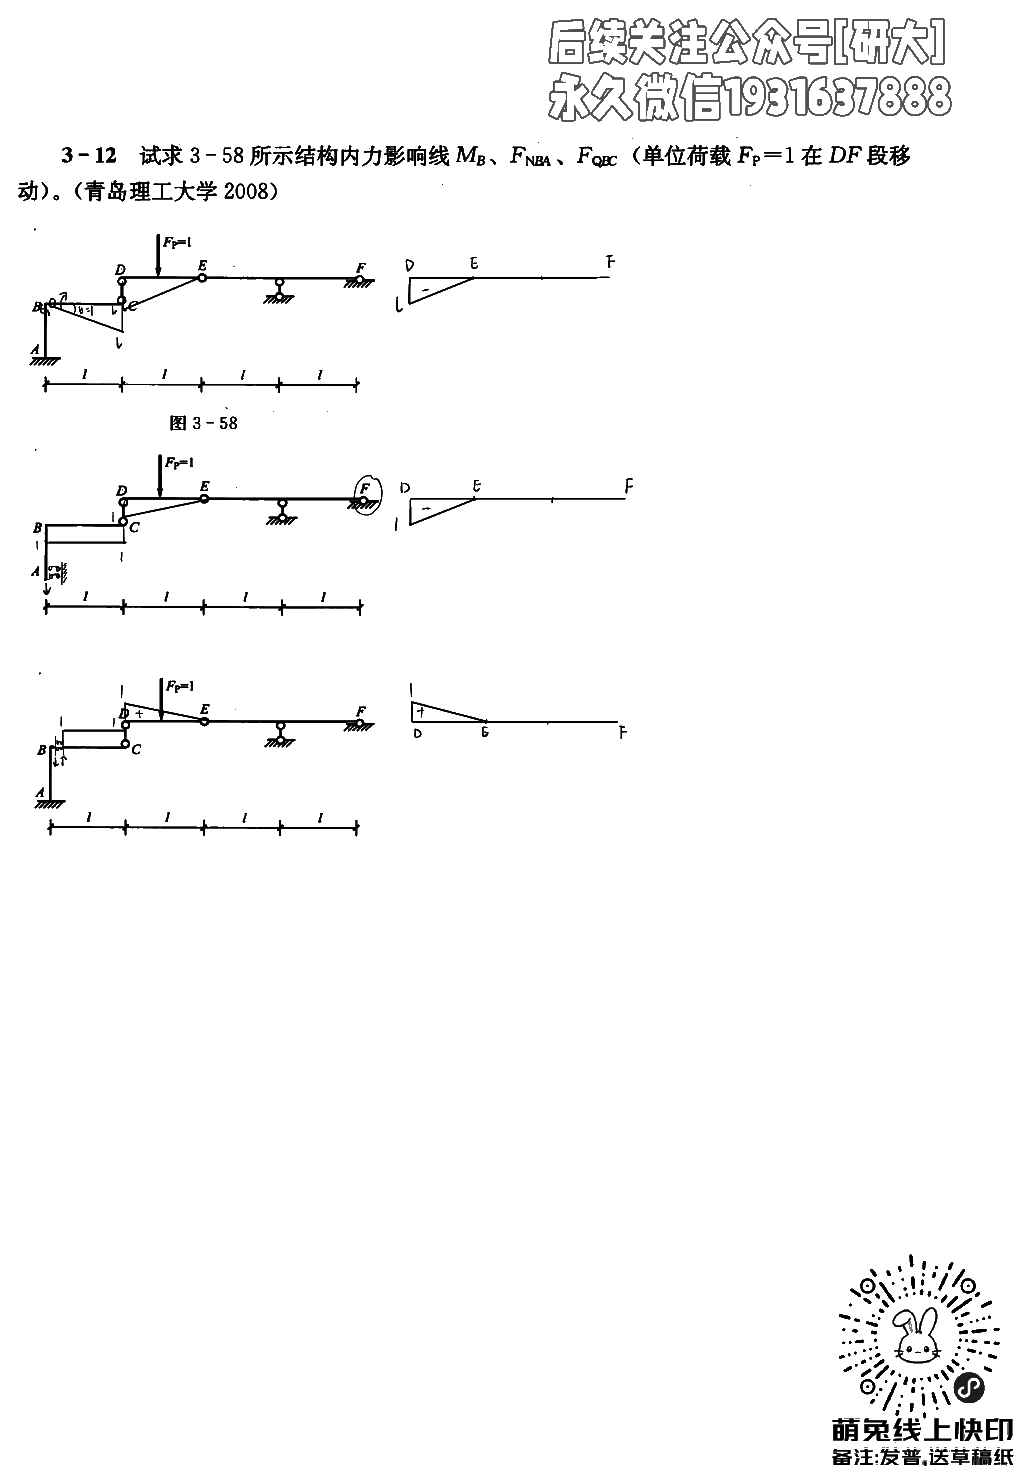
\includegraphics[width=0.96\textwidth,height=0.82\textheight,keepaspectratio]{images/c08_note_p09.png}
\par\small 讲解笔记（去水印版），第 9/11 页
\end{center}
\clearpage
\begin{center}
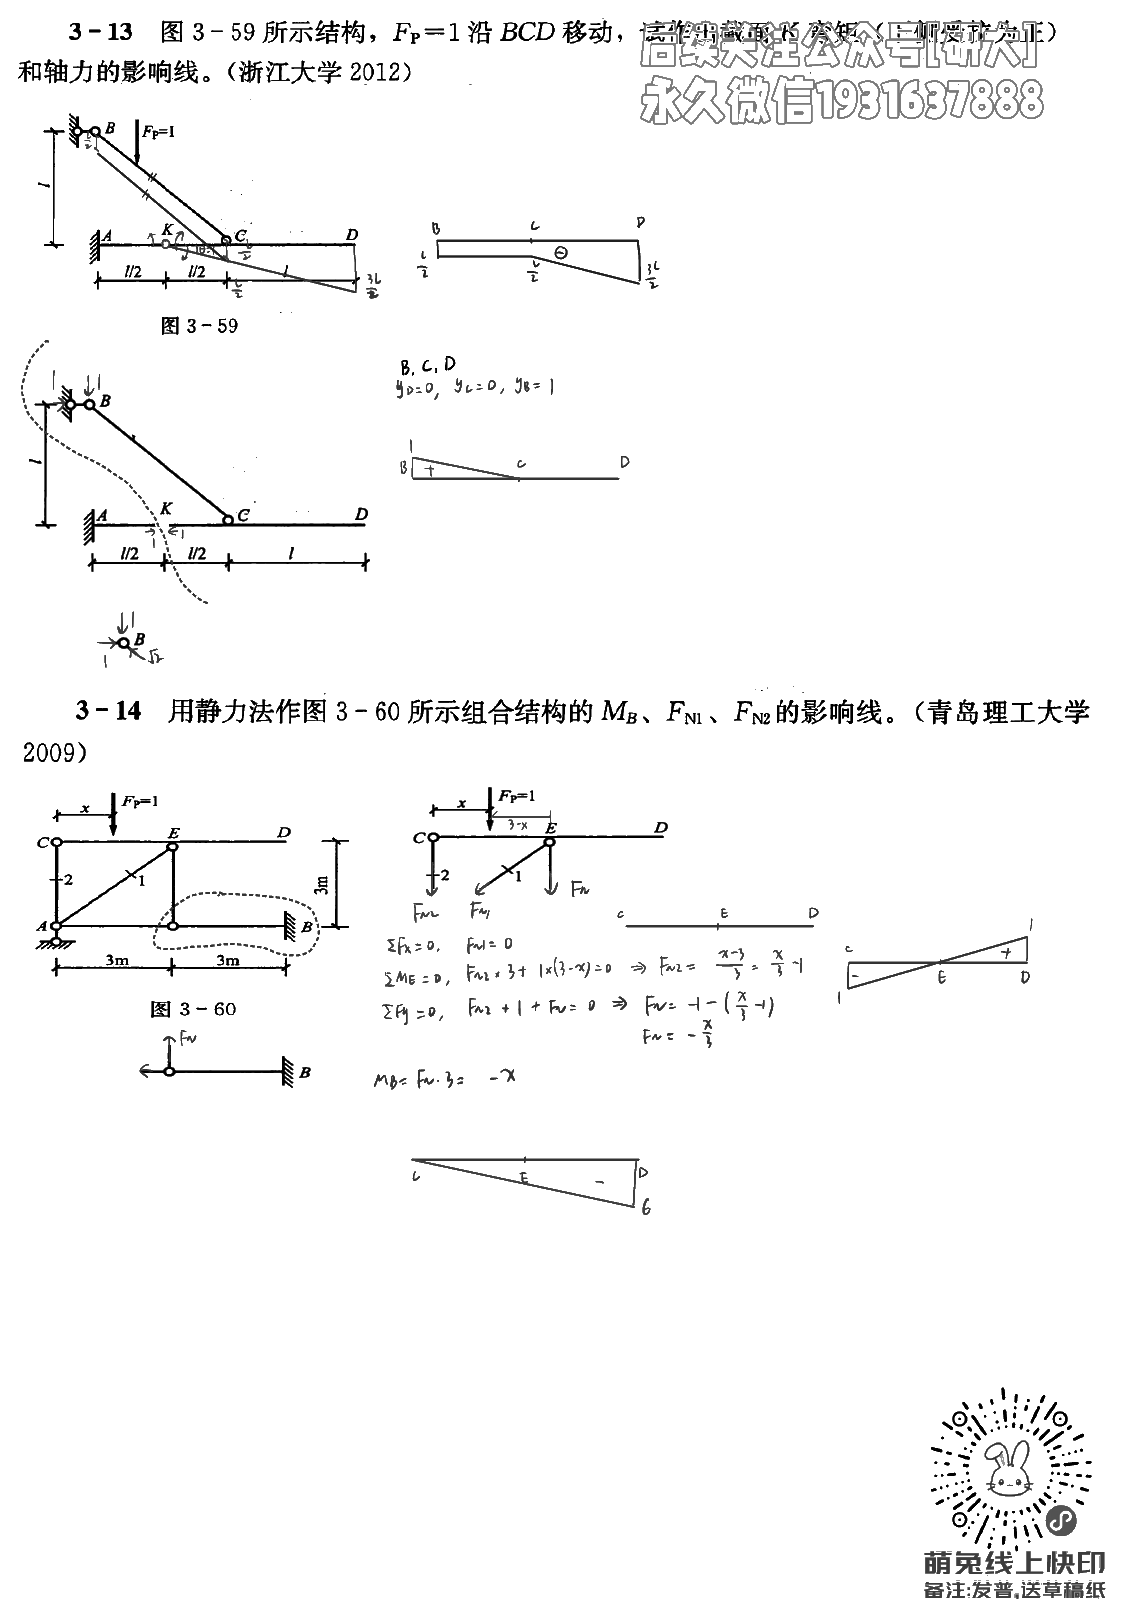
\includegraphics[width=0.96\textwidth,height=0.82\textheight,keepaspectratio]{images/c08_note_p10.png}
\par\small 讲解笔记（去水印版），第 10/11 页
\end{center}
\clearpage
\begin{center}
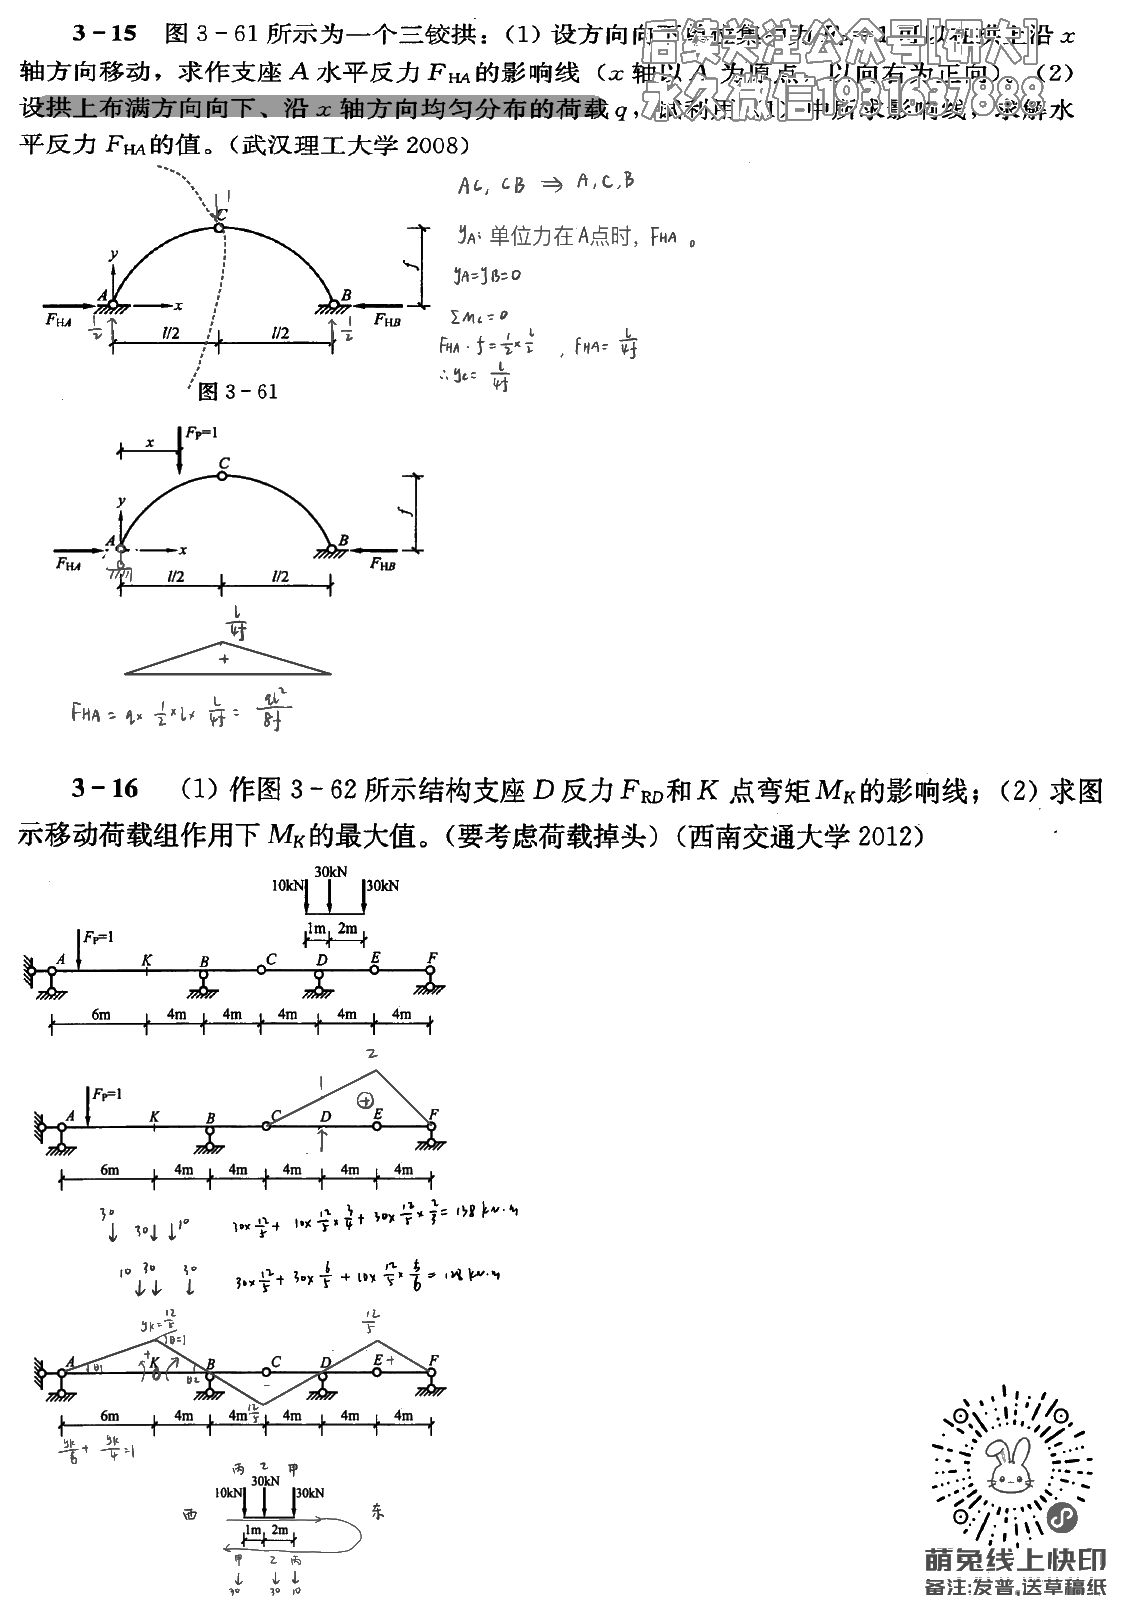
\includegraphics[width=0.96\textwidth,height=0.82\textheight,keepaspectratio]{images/c08_note_p11.png}
\par\small 讲解笔记（去水印版），第 11/11 页
\end{center}
\clearpage
\chapter{第9讲：静定结构位移计算}
\begin{tcolorbox}[title=解析要点]
位移计算以虚功原理为主线。单位荷载法中，实际荷载弯矩图 $M$ 与单位荷载弯矩图 $\overline M$ 的图乘或积分给出目标位移。
\end{tcolorbox}
\begin{tcolorbox}[title=答案与校核]
答案页给出位移计算结果；注意实际弯矩图和单位弯矩图的乘积符号。
\end{tcolorbox}
\section{作业与答案（去水印版）}
\begin{center}
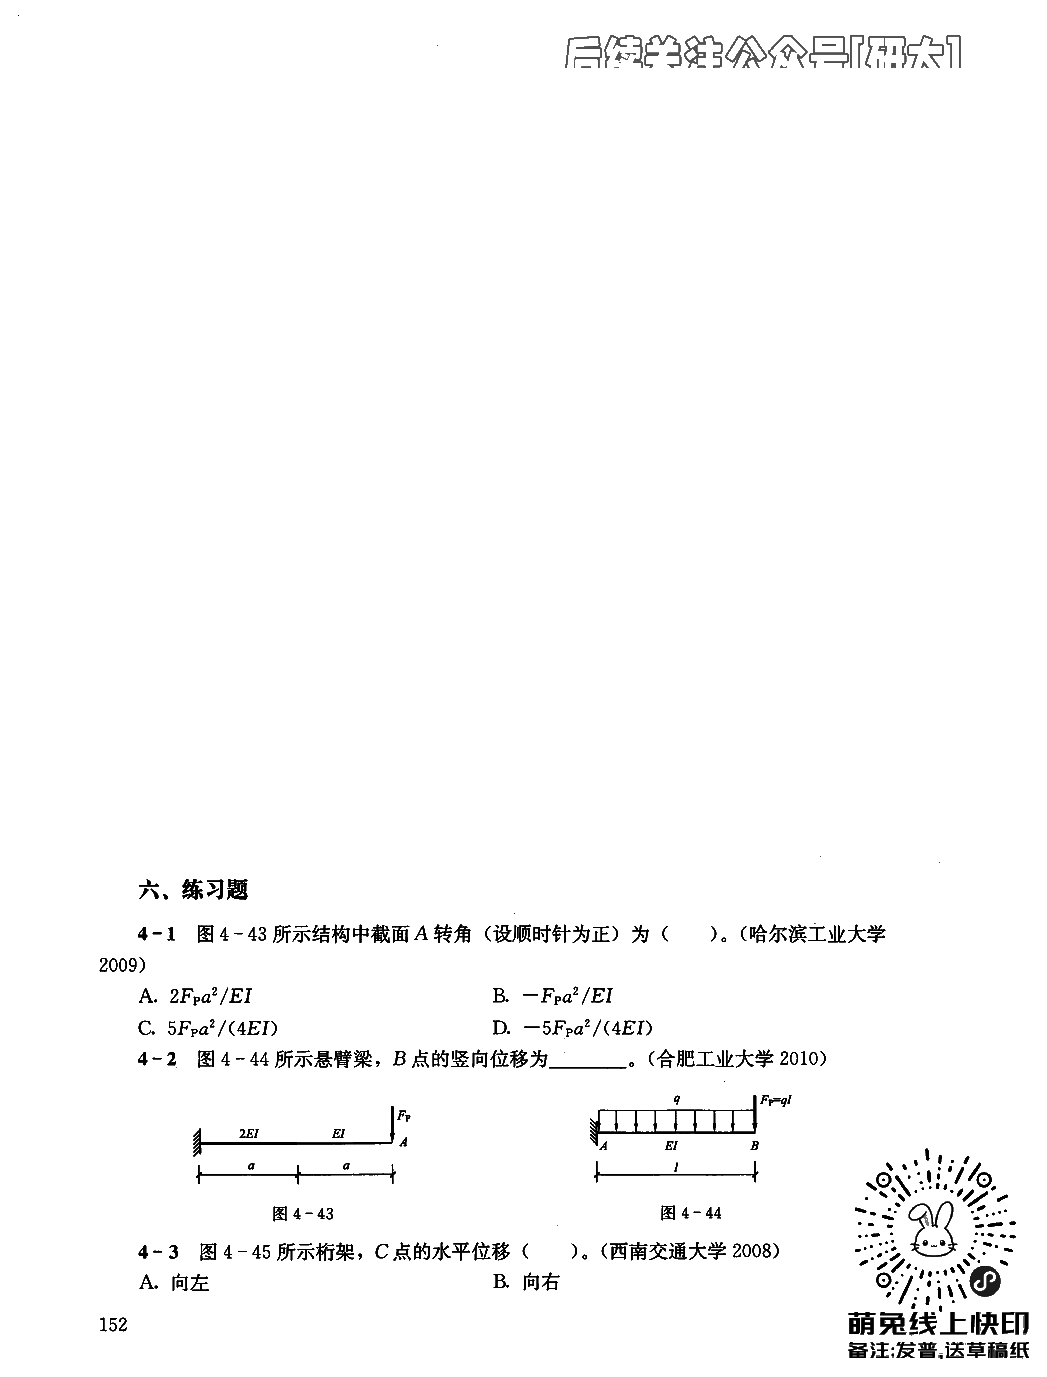
\includegraphics[width=0.96\textwidth,height=0.82\textheight,keepaspectratio]{images/c09_answer_1_p01.png}
\par\small 作业与答案（去水印版），第 1/4 页
\end{center}
\clearpage
\begin{center}
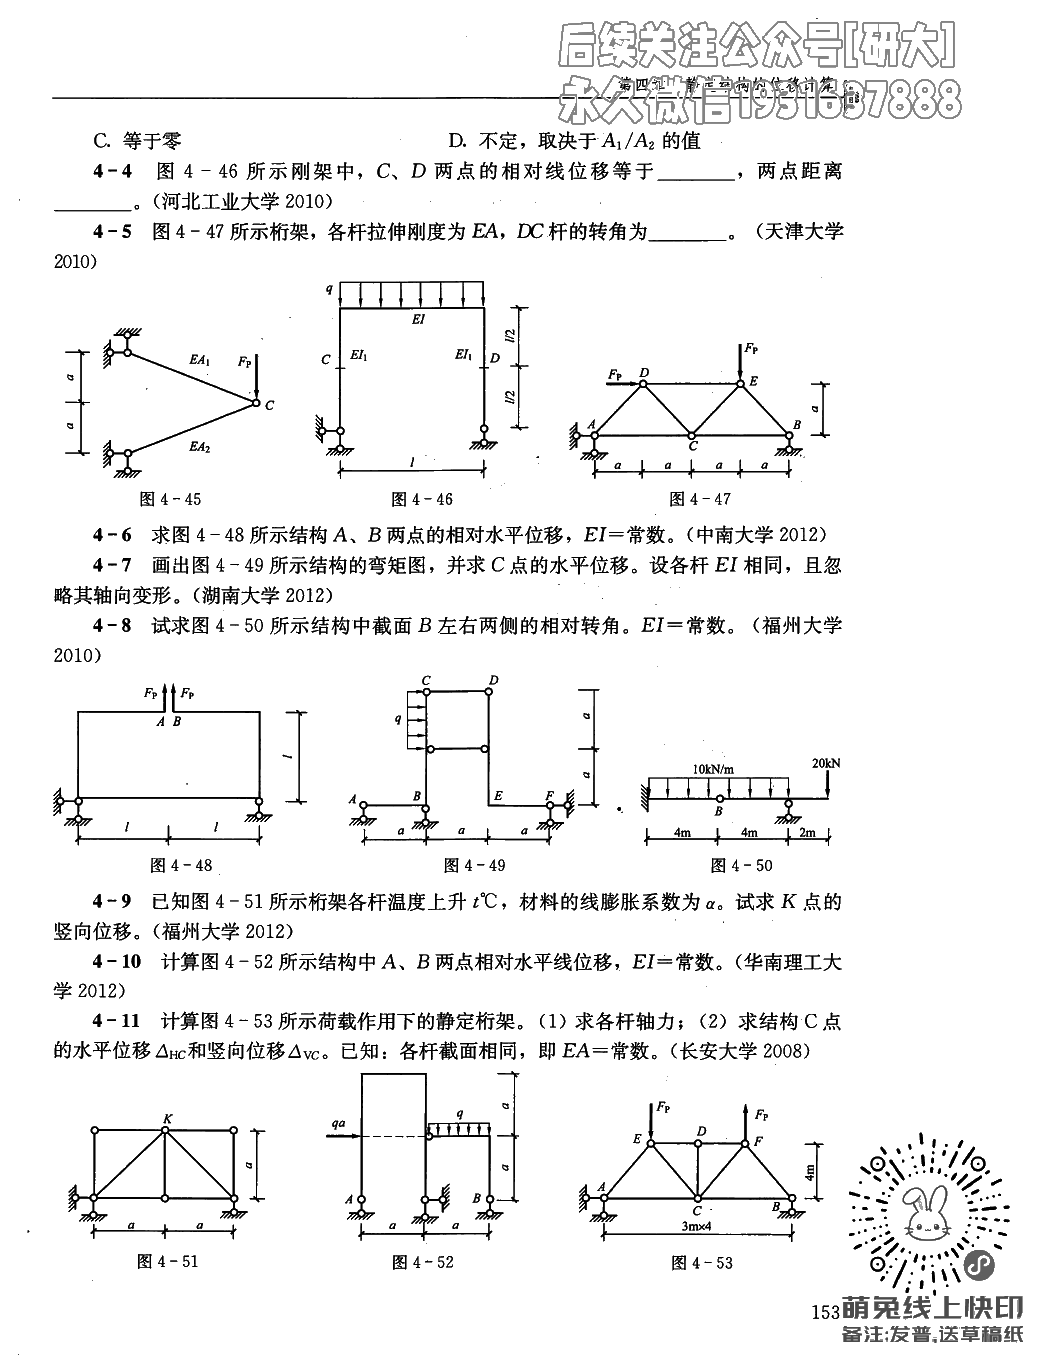
\includegraphics[width=0.96\textwidth,height=0.82\textheight,keepaspectratio]{images/c09_answer_1_p02.png}
\par\small 作业与答案（去水印版），第 2/4 页
\end{center}
\clearpage
\begin{center}
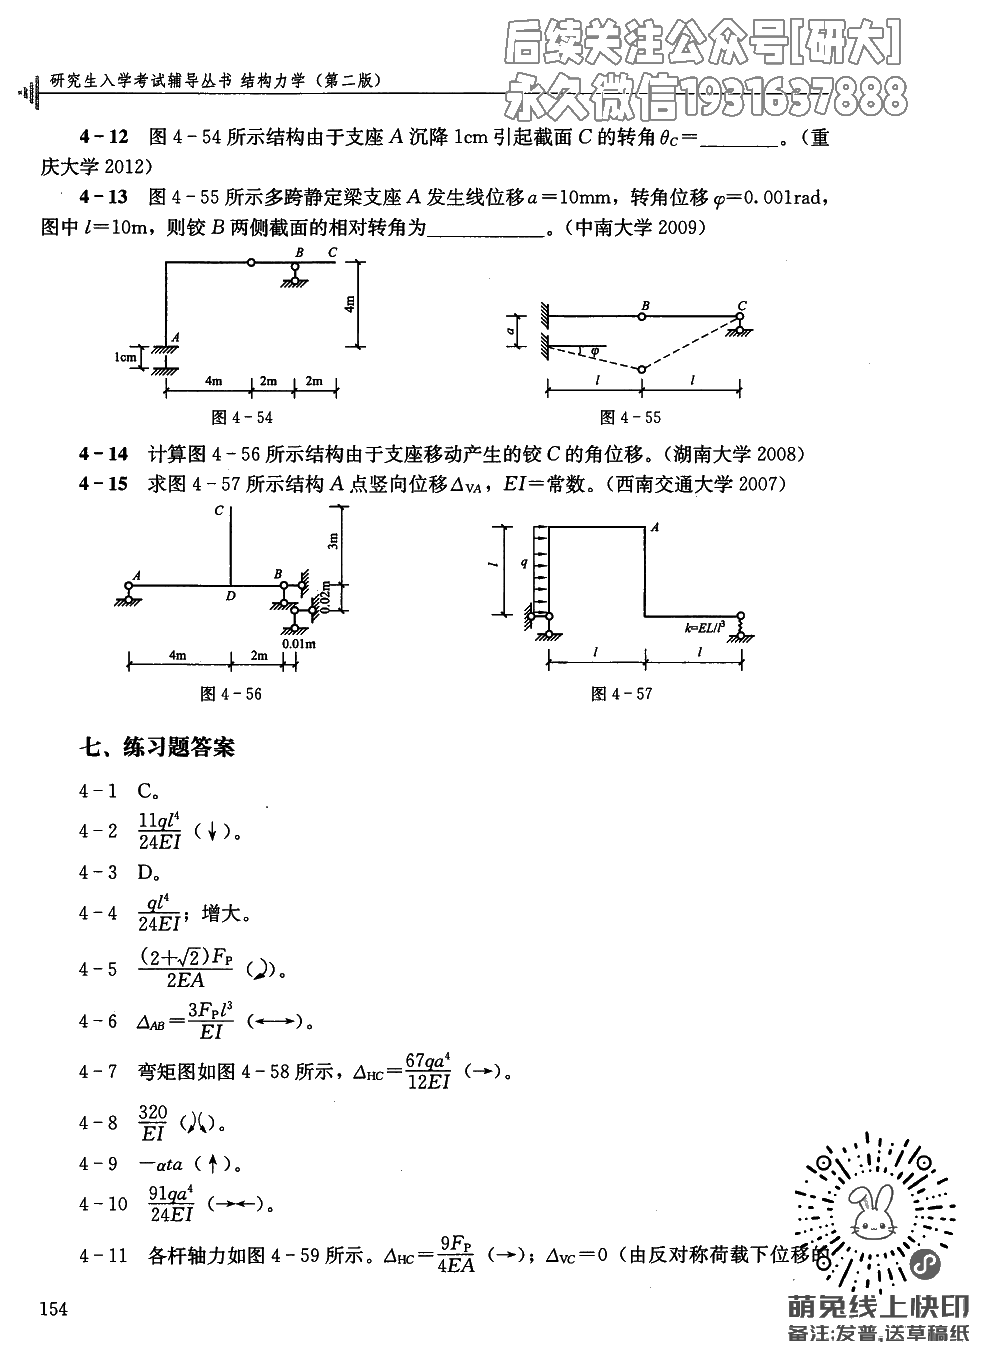
\includegraphics[width=0.96\textwidth,height=0.82\textheight,keepaspectratio]{images/c09_answer_1_p03.png}
\par\small 作业与答案（去水印版），第 3/4 页
\end{center}
\clearpage
\begin{center}
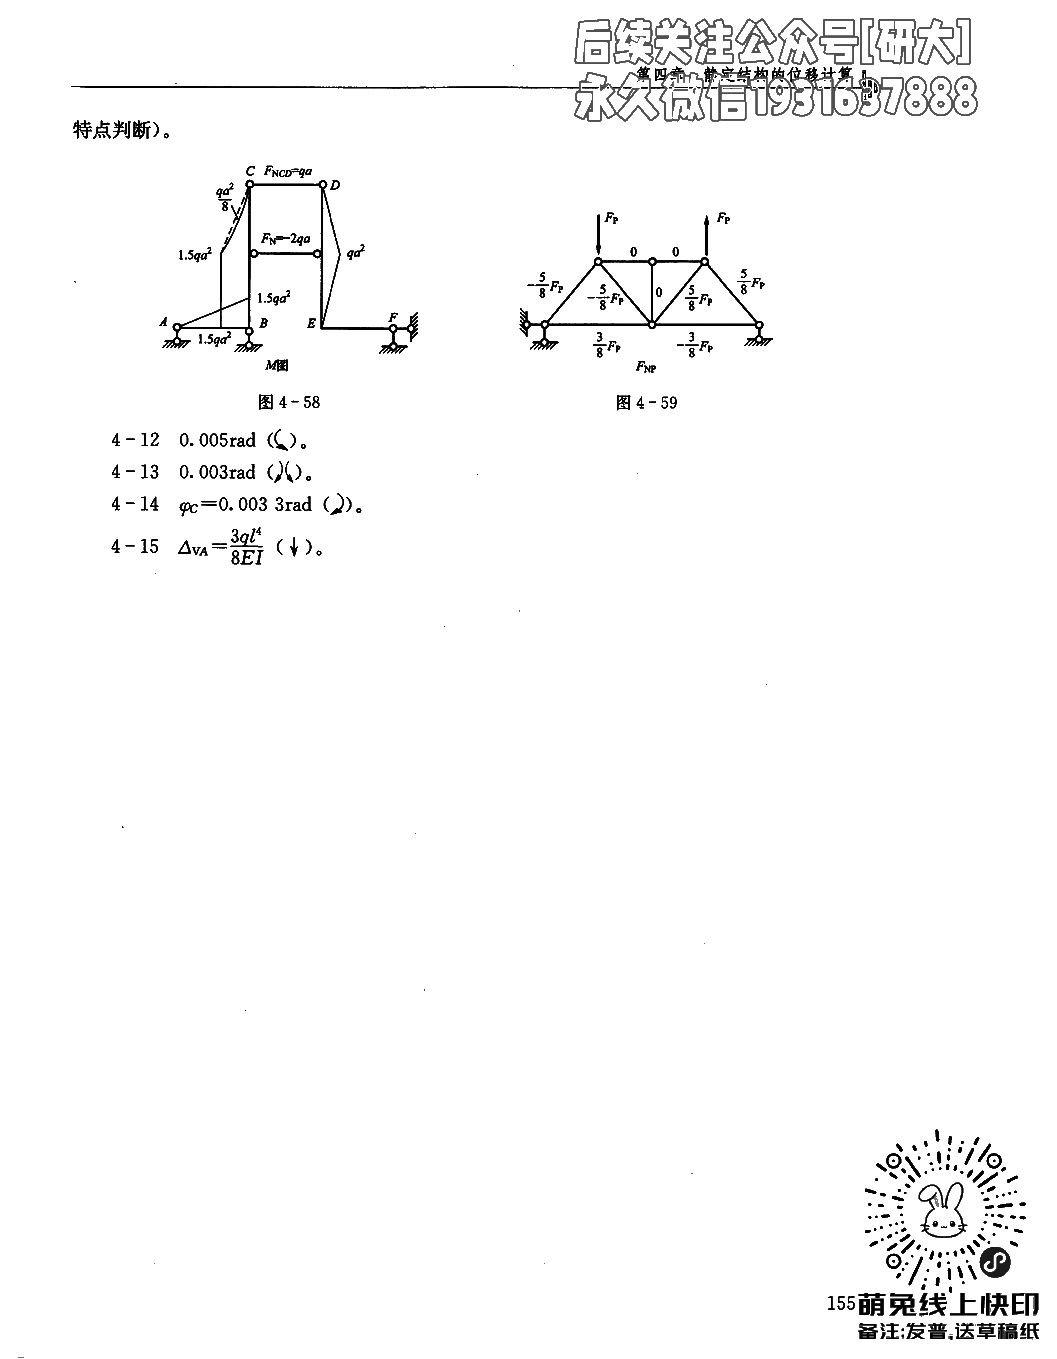
\includegraphics[width=0.96\textwidth,height=0.82\textheight,keepaspectratio]{images/c09_answer_1_p04.png}
\par\small 作业与答案（去水印版），第 4/4 页
\end{center}
\clearpage
\section{讲解笔记（去水印版）}
\begin{center}
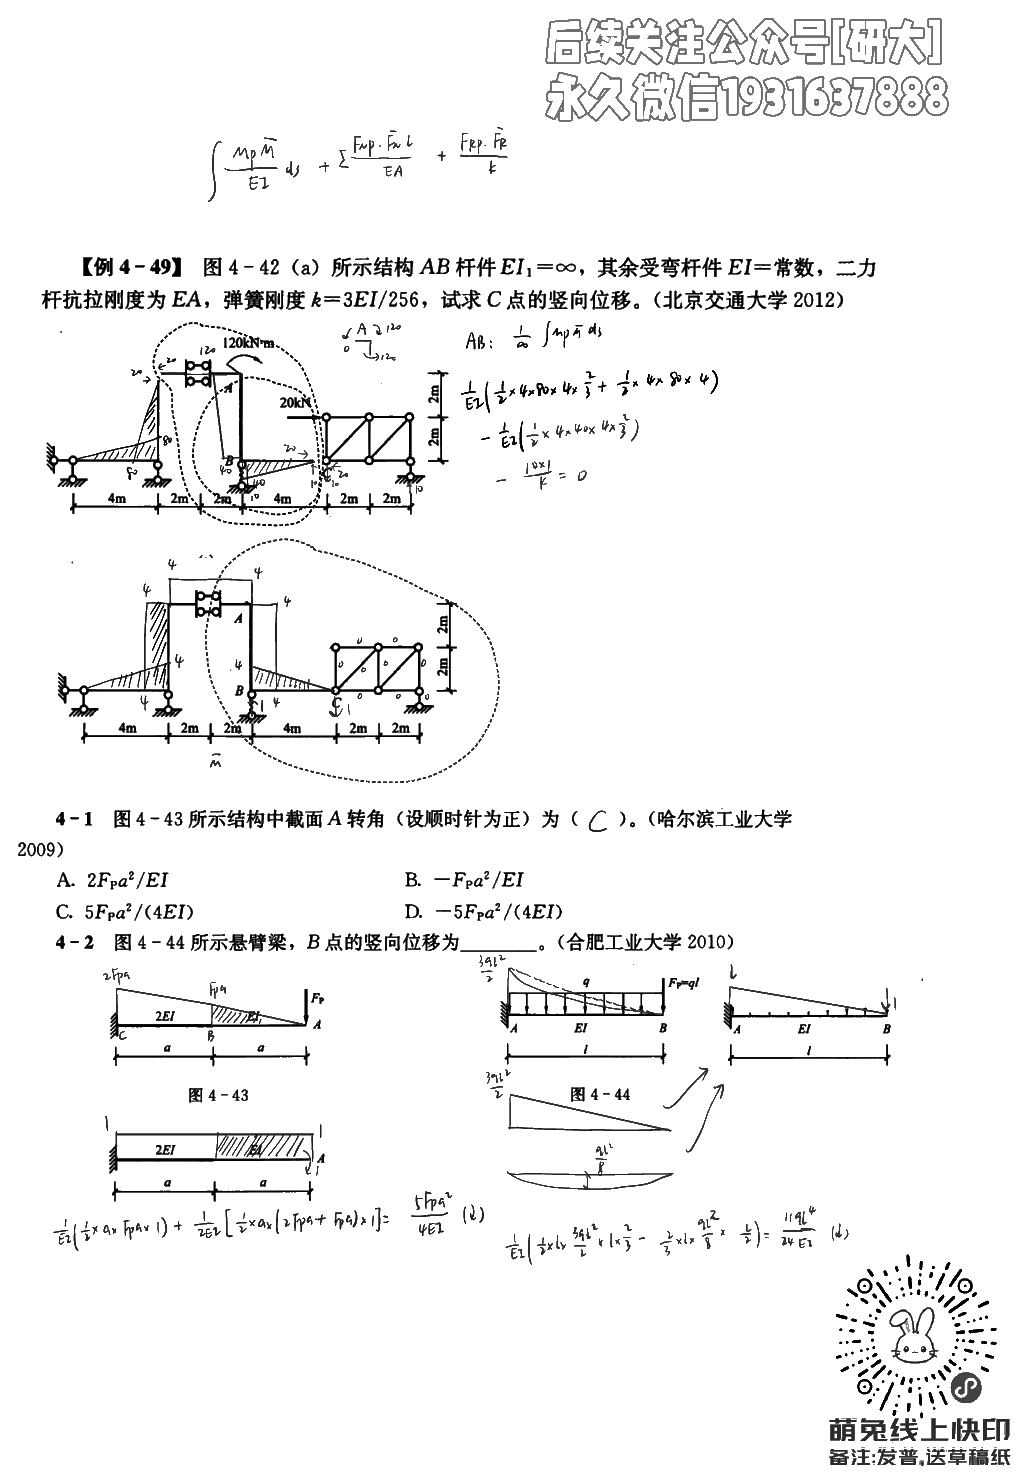
\includegraphics[width=0.96\textwidth,height=0.82\textheight,keepaspectratio]{images/c09_note_p01.png}
\par\small 讲解笔记（去水印版），第 1/5 页
\end{center}
\clearpage
\begin{center}
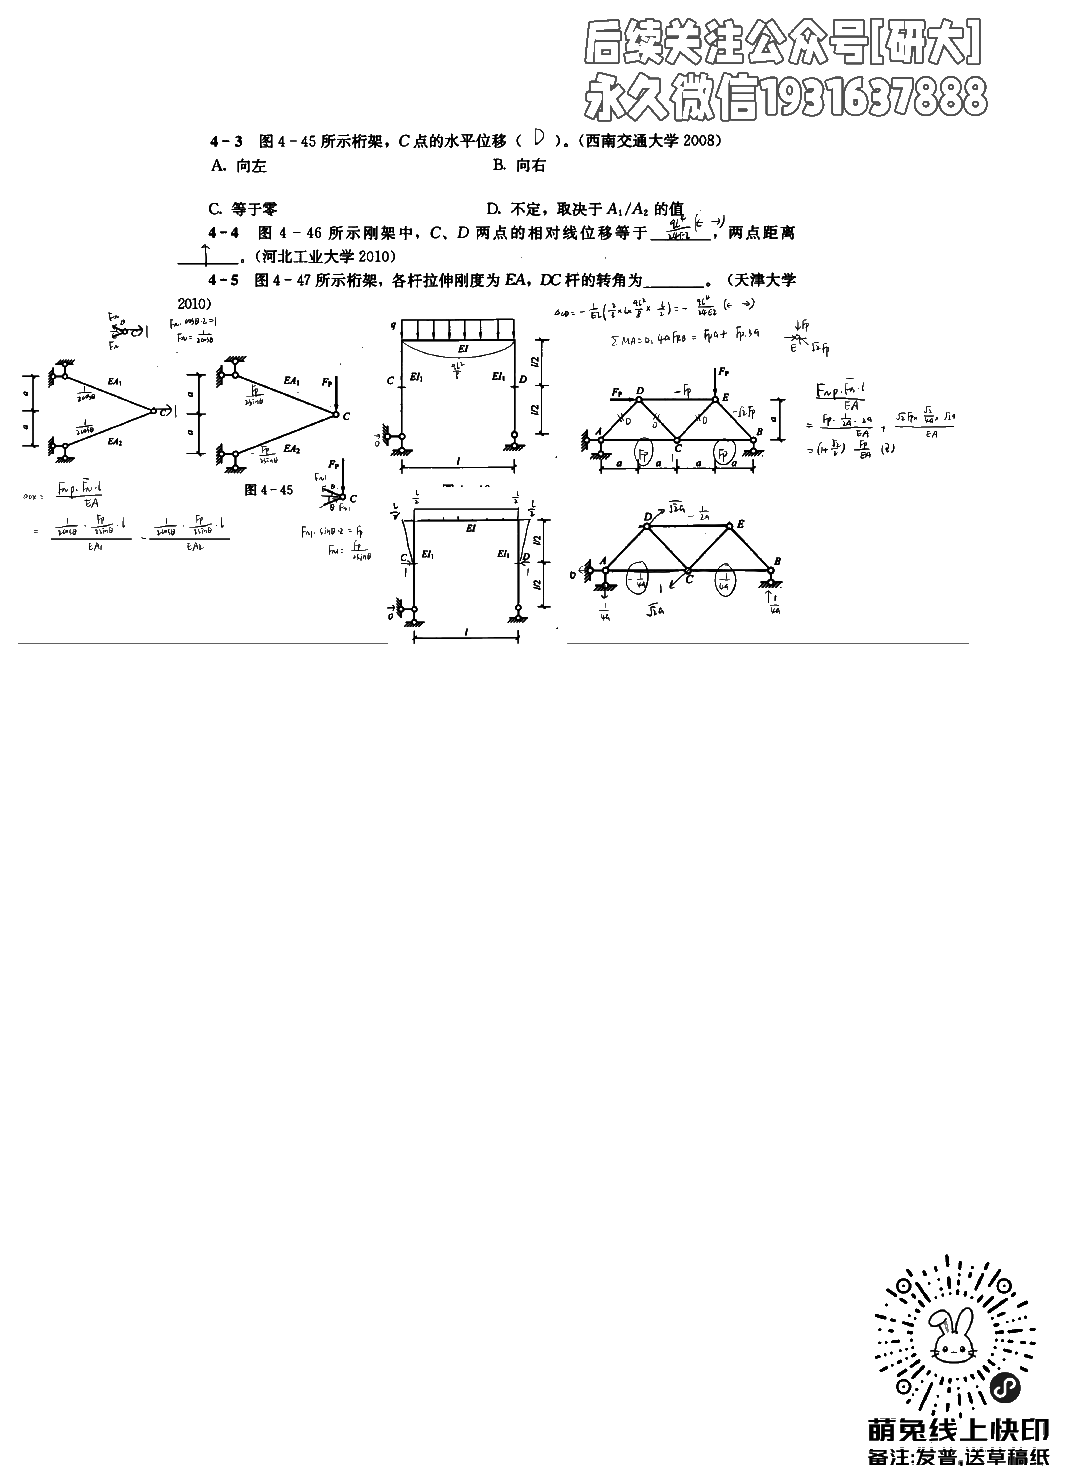
\includegraphics[width=0.96\textwidth,height=0.82\textheight,keepaspectratio]{images/c09_note_p02.png}
\par\small 讲解笔记（去水印版），第 2/5 页
\end{center}
\clearpage
\begin{center}
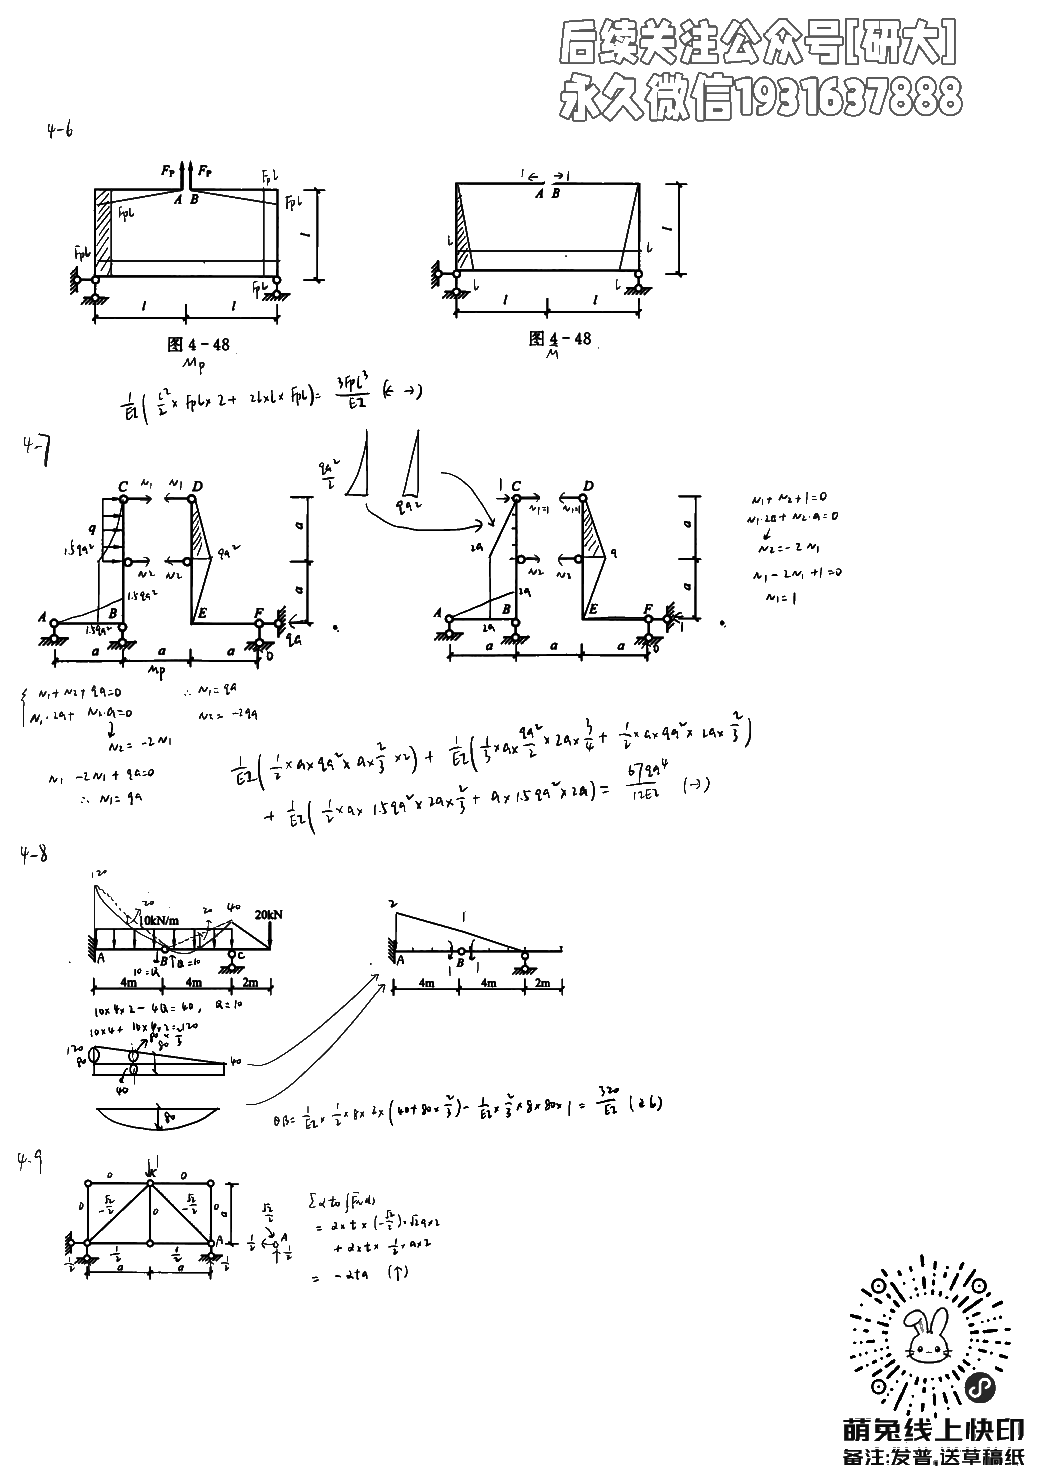
\includegraphics[width=0.96\textwidth,height=0.82\textheight,keepaspectratio]{images/c09_note_p03.png}
\par\small 讲解笔记（去水印版），第 3/5 页
\end{center}
\clearpage
\begin{center}
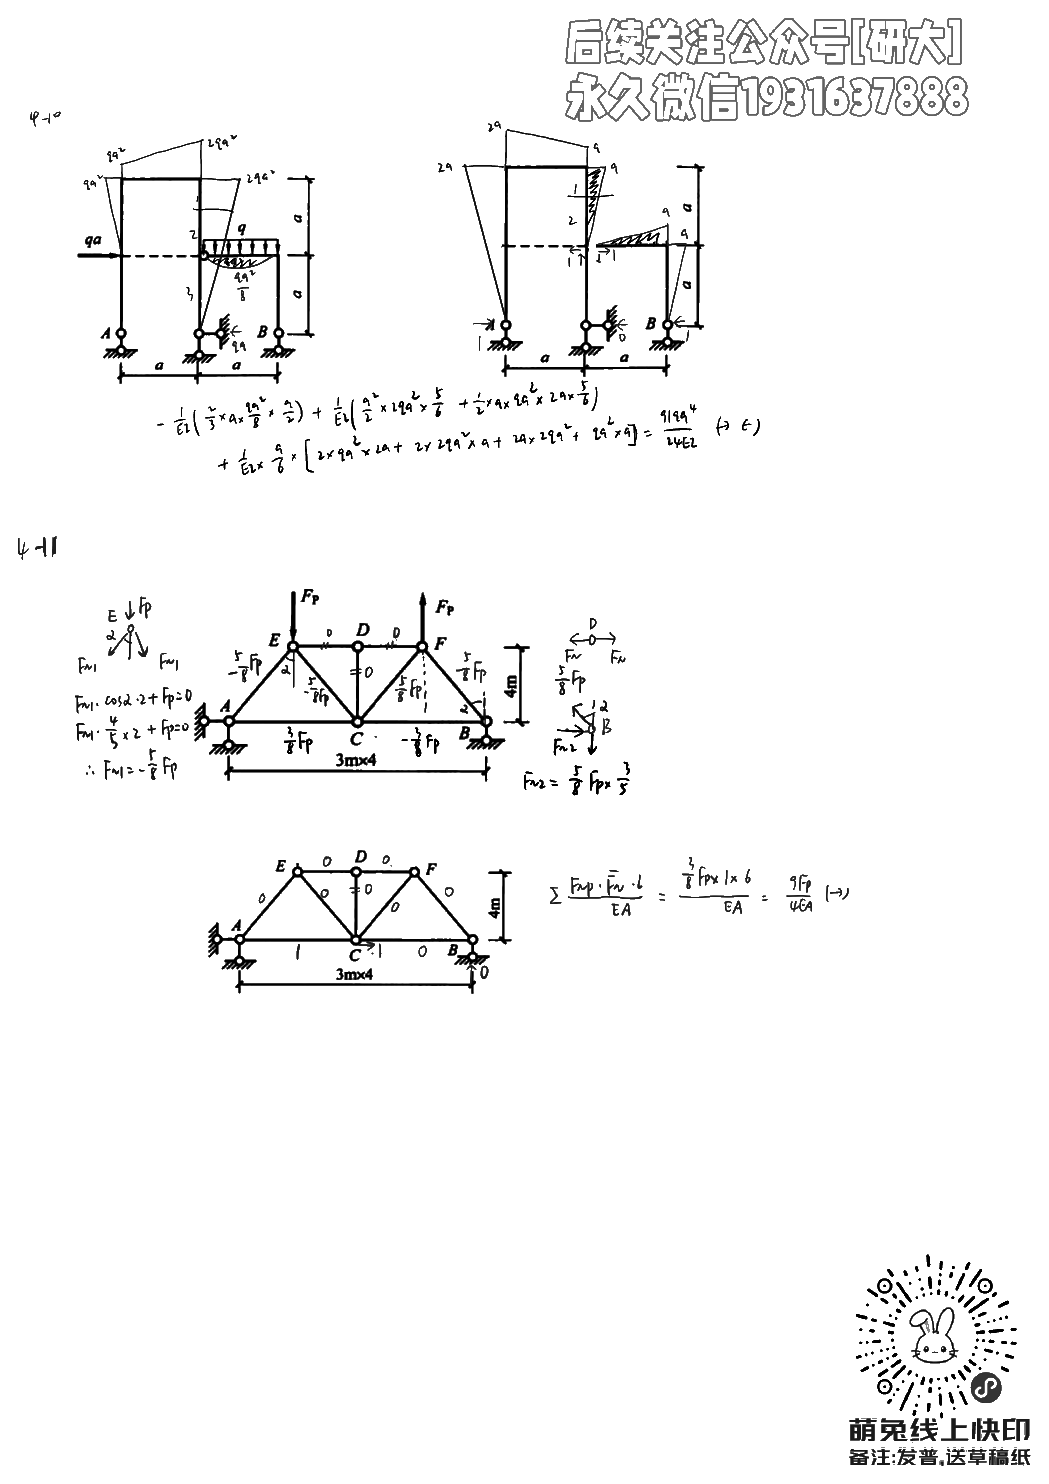
\includegraphics[width=0.96\textwidth,height=0.82\textheight,keepaspectratio]{images/c09_note_p04.png}
\par\small 讲解笔记（去水印版），第 4/5 页
\end{center}
\clearpage
\begin{center}
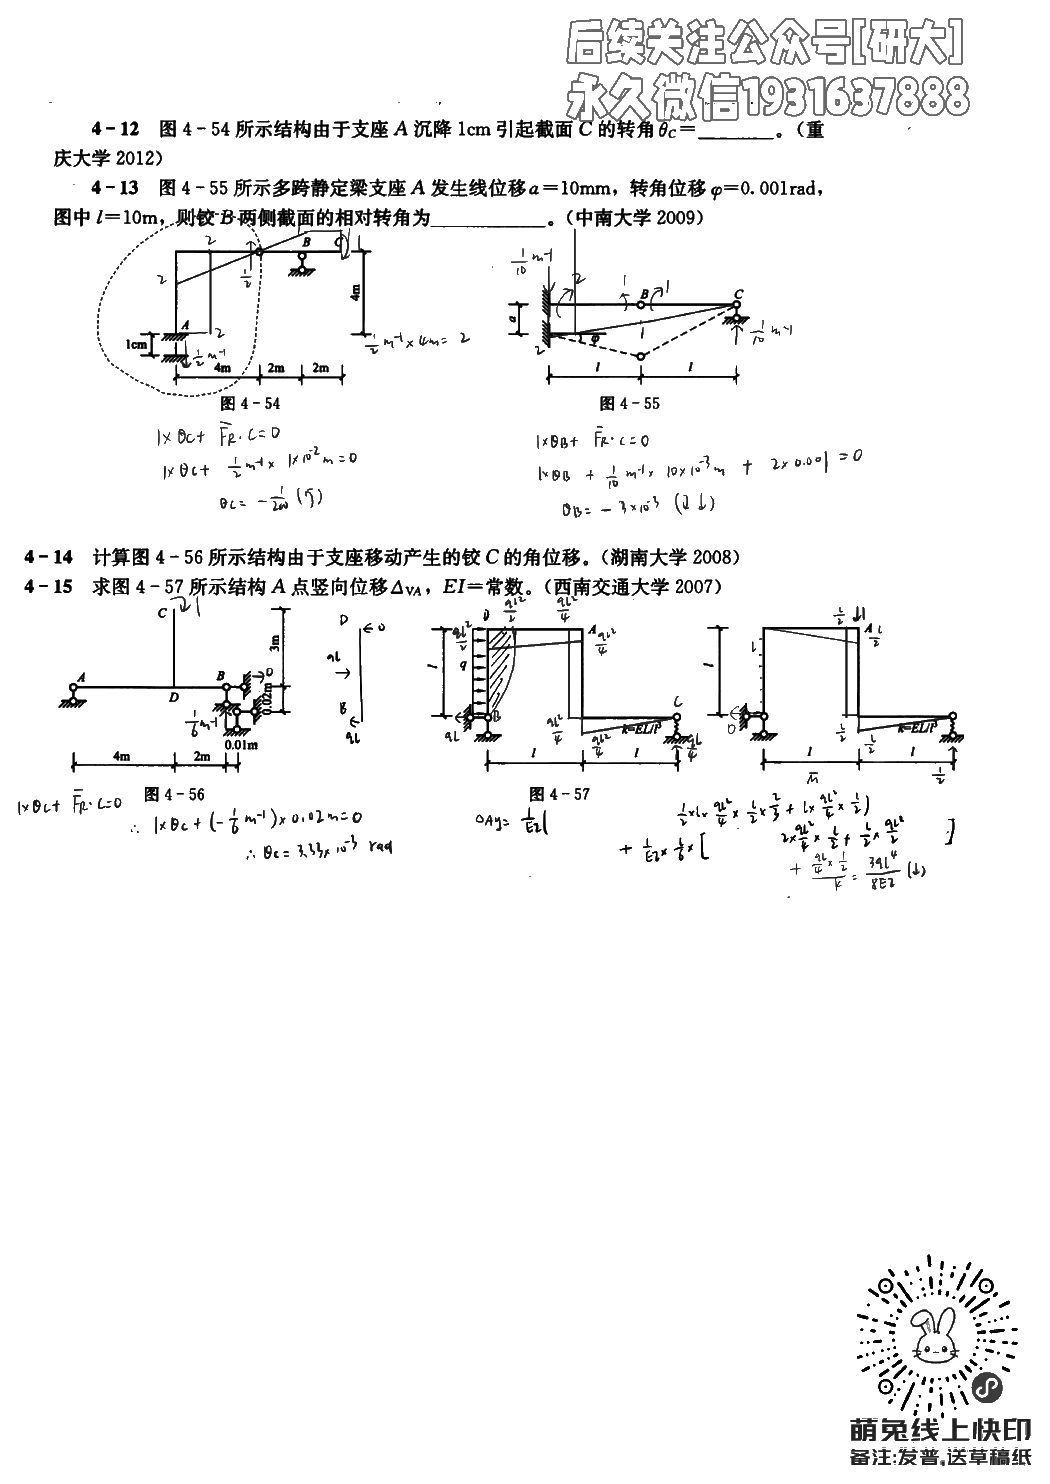
\includegraphics[width=0.96\textwidth,height=0.82\textheight,keepaspectratio]{images/c09_note_p05.png}
\par\small 讲解笔记（去水印版），第 5/5 页
\end{center}
\clearpage
\chapter{第10讲：力法（一）}
\begin{tcolorbox}[title=解析要点]
力法先确定超静定次数，选择赘余力并建立基本体系。柔度方程表达的是赘余力方向上的变形协调，最后叠加荷载效应与赘余力效应。
\end{tcolorbox}
\begin{tcolorbox}[title=答案与校核]
答案页给出力法（一）的柔度方程和赘余力；最终内力由基本体系叠加得到。
\end{tcolorbox}
\section{作业与答案（去水印版）}
\begin{center}
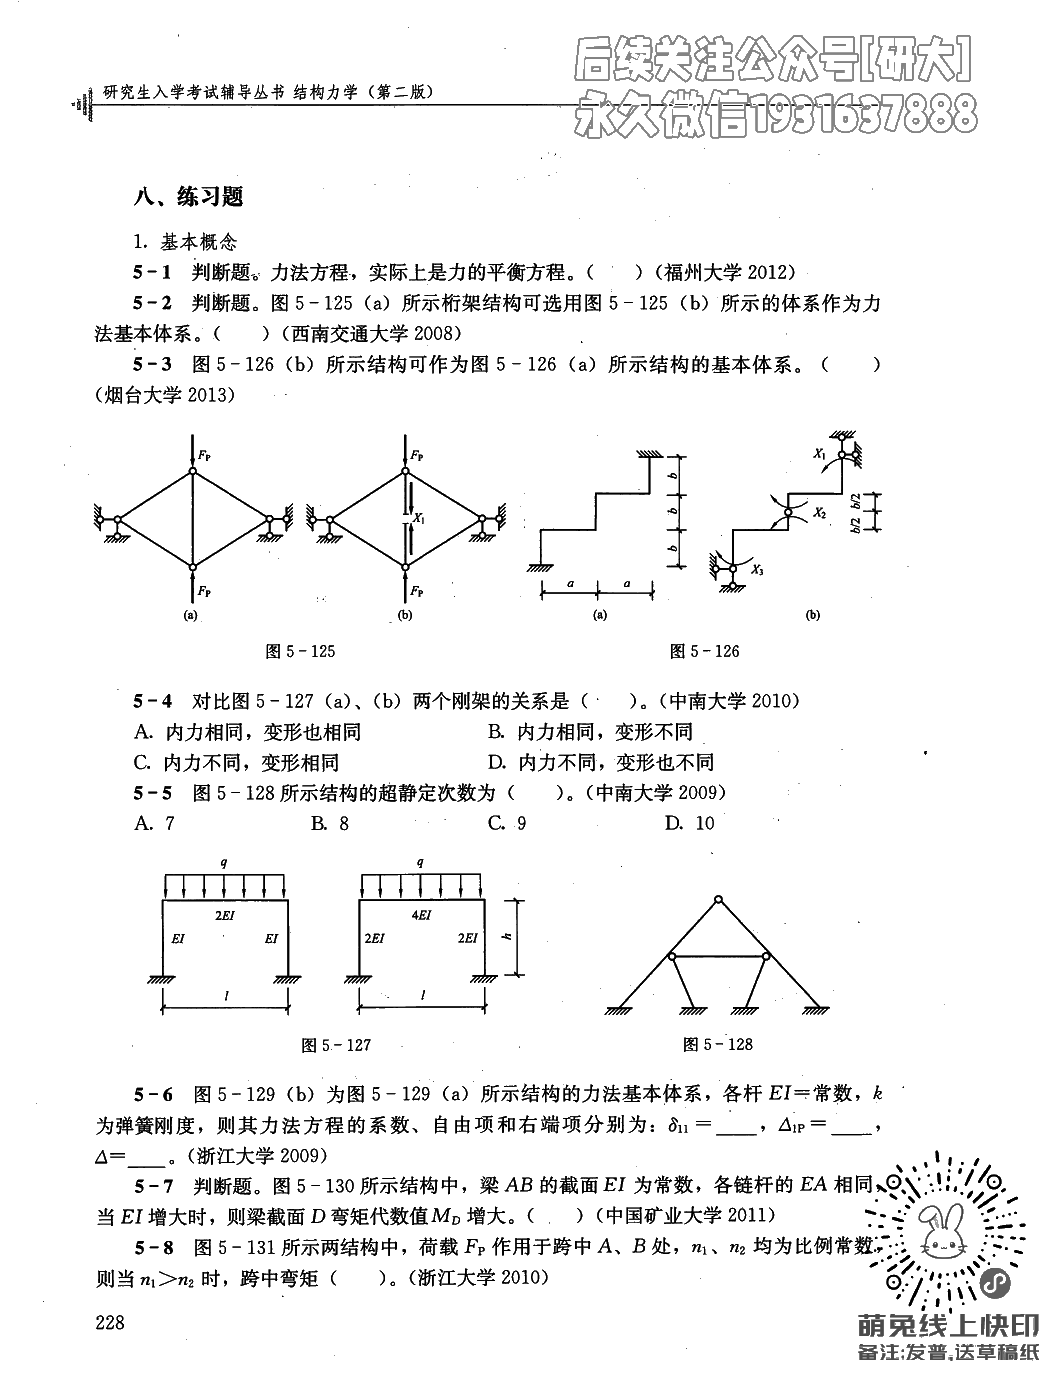
\includegraphics[width=0.96\textwidth,height=0.82\textheight,keepaspectratio]{images/c10_answer_1_p01.png}
\par\small 作业与答案（去水印版），第 1/21 页
\end{center}
\clearpage
\begin{center}
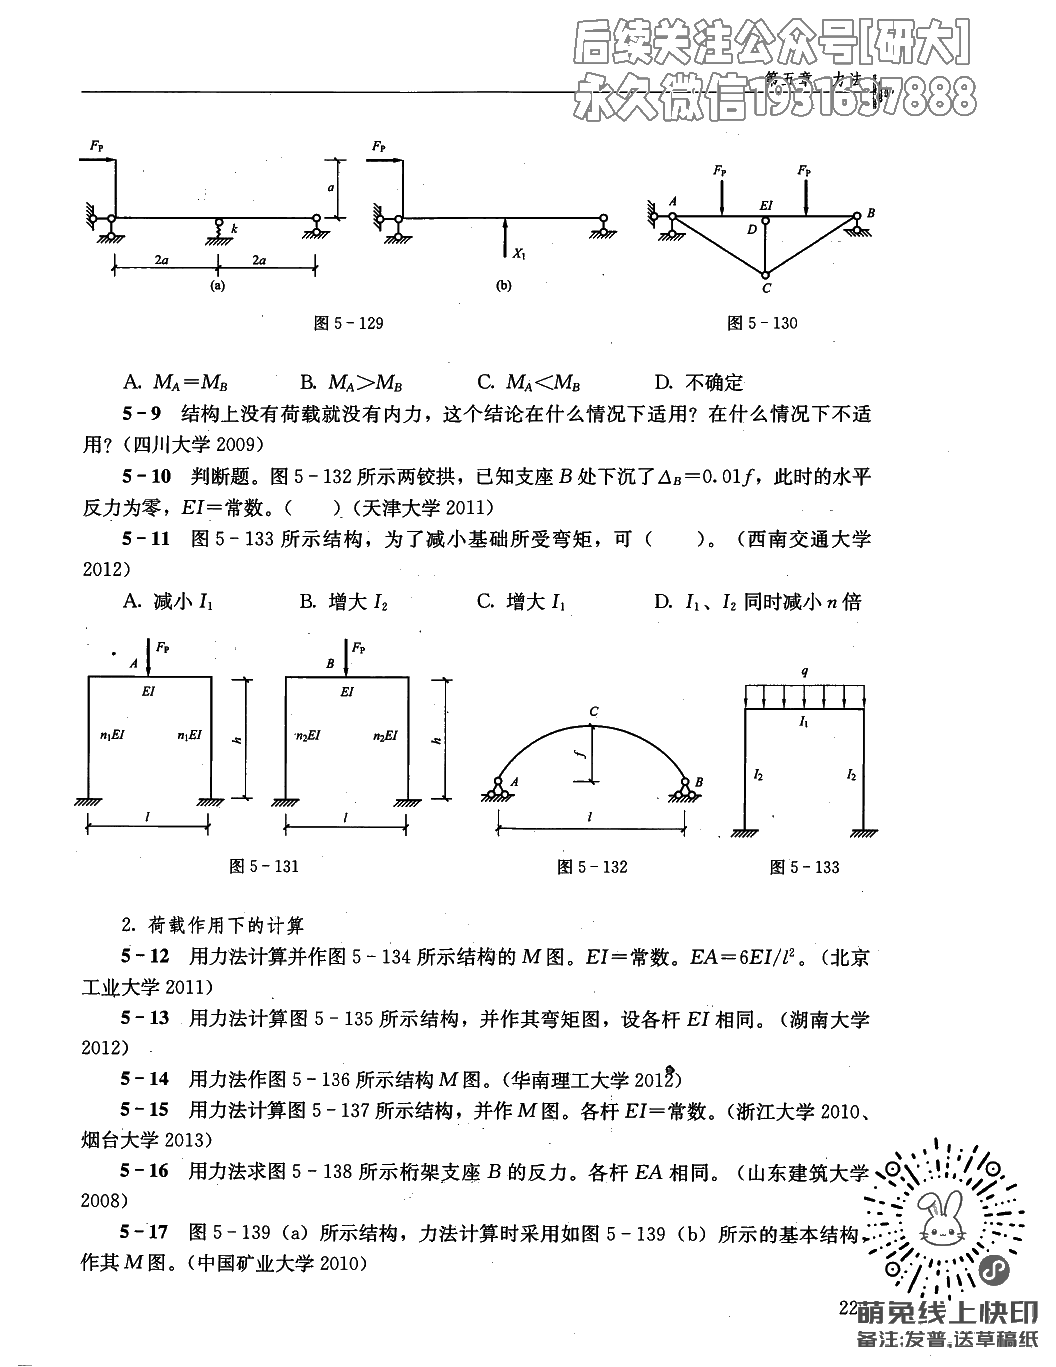
\includegraphics[width=0.96\textwidth,height=0.82\textheight,keepaspectratio]{images/c10_answer_1_p02.png}
\par\small 作业与答案（去水印版），第 2/21 页
\end{center}
\clearpage
\begin{center}
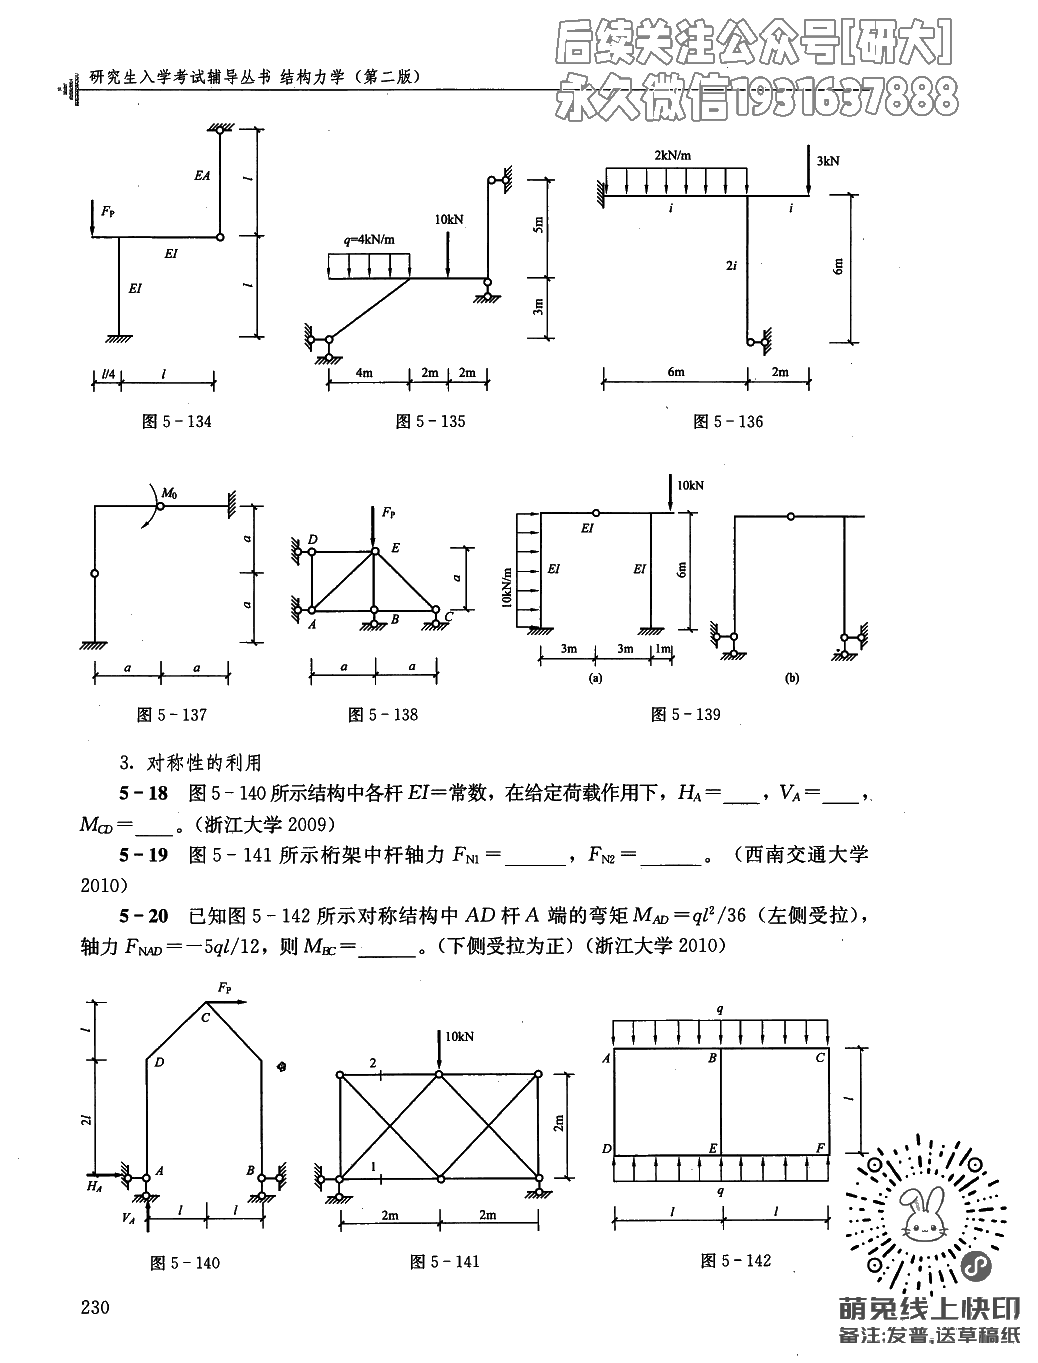
\includegraphics[width=0.96\textwidth,height=0.82\textheight,keepaspectratio]{images/c10_answer_1_p03.png}
\par\small 作业与答案（去水印版），第 3/21 页
\end{center}
\clearpage
\begin{center}
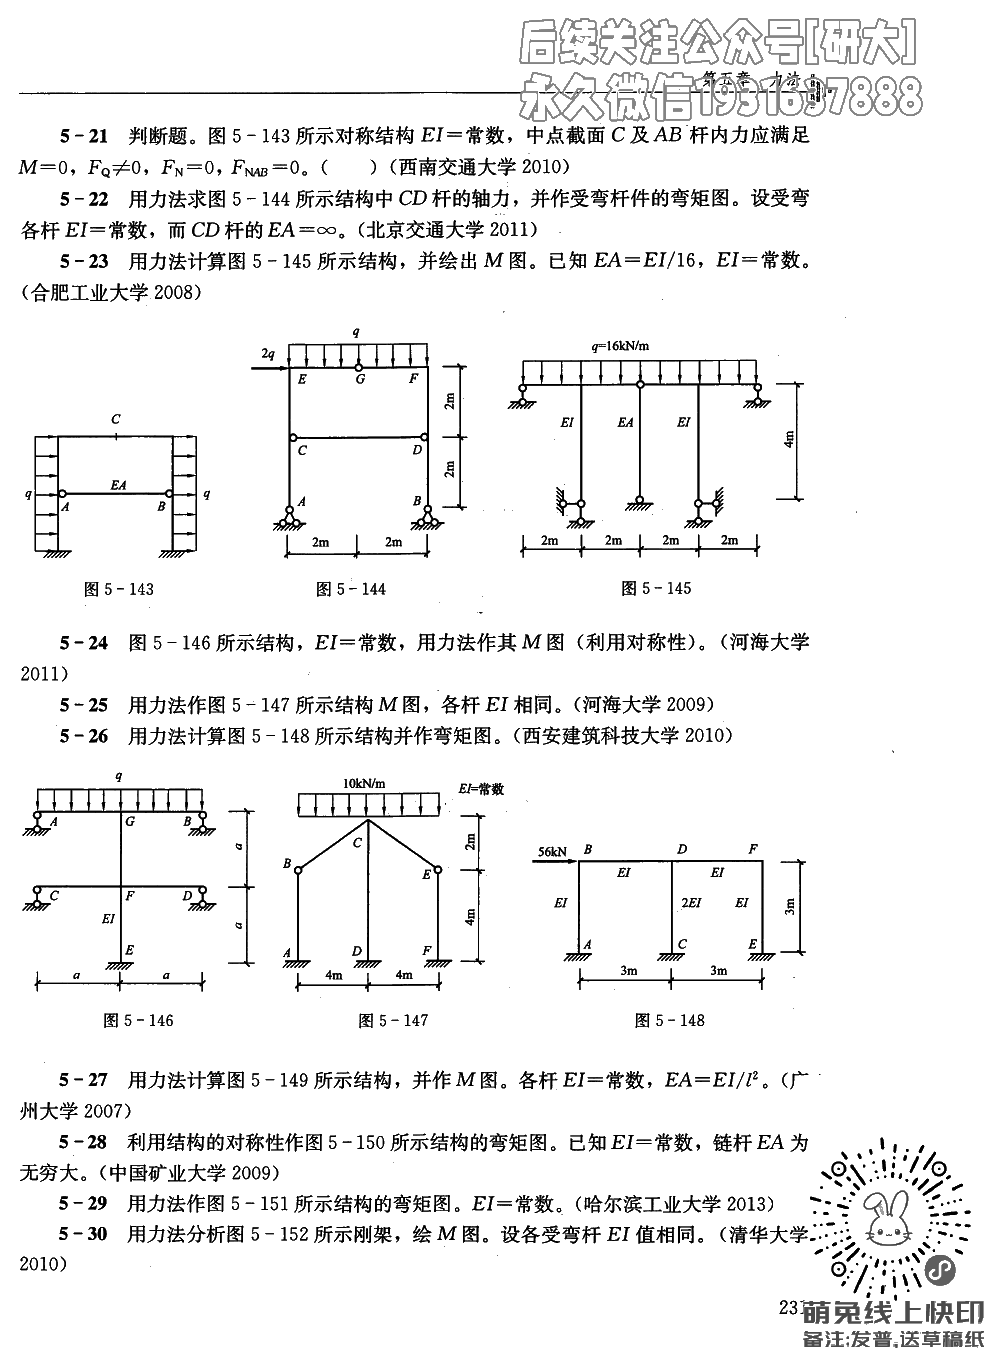
\includegraphics[width=0.96\textwidth,height=0.82\textheight,keepaspectratio]{images/c10_answer_1_p04.png}
\par\small 作业与答案（去水印版），第 4/21 页
\end{center}
\clearpage
\begin{center}
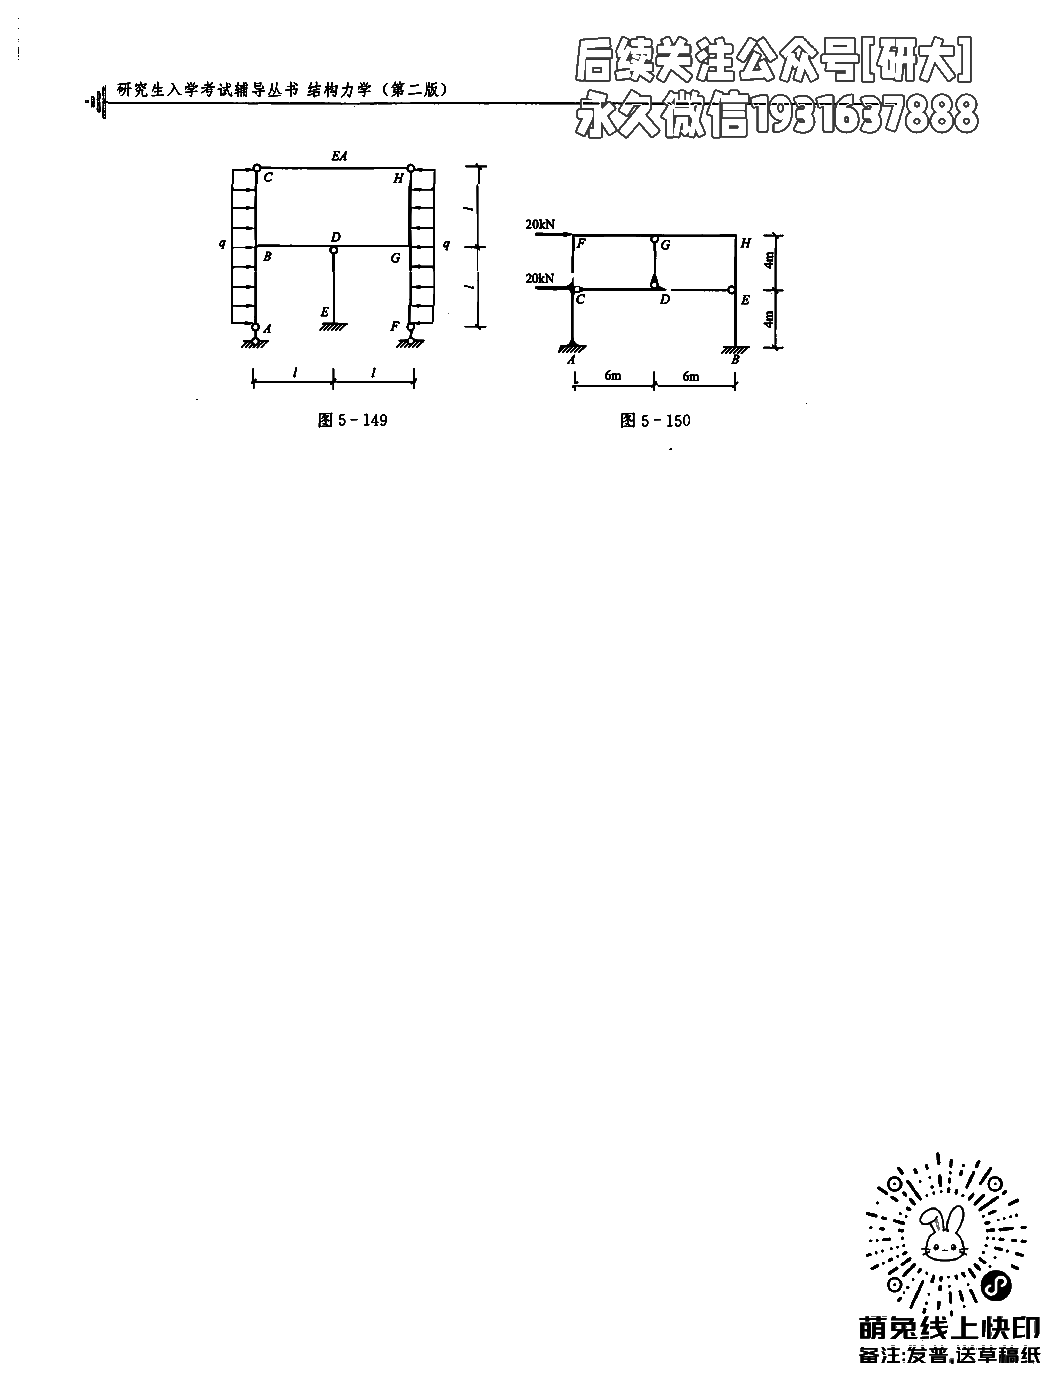
\includegraphics[width=0.96\textwidth,height=0.82\textheight,keepaspectratio]{images/c10_answer_1_p05.png}
\par\small 作业与答案（去水印版），第 5/21 页
\end{center}
\clearpage
\begin{center}
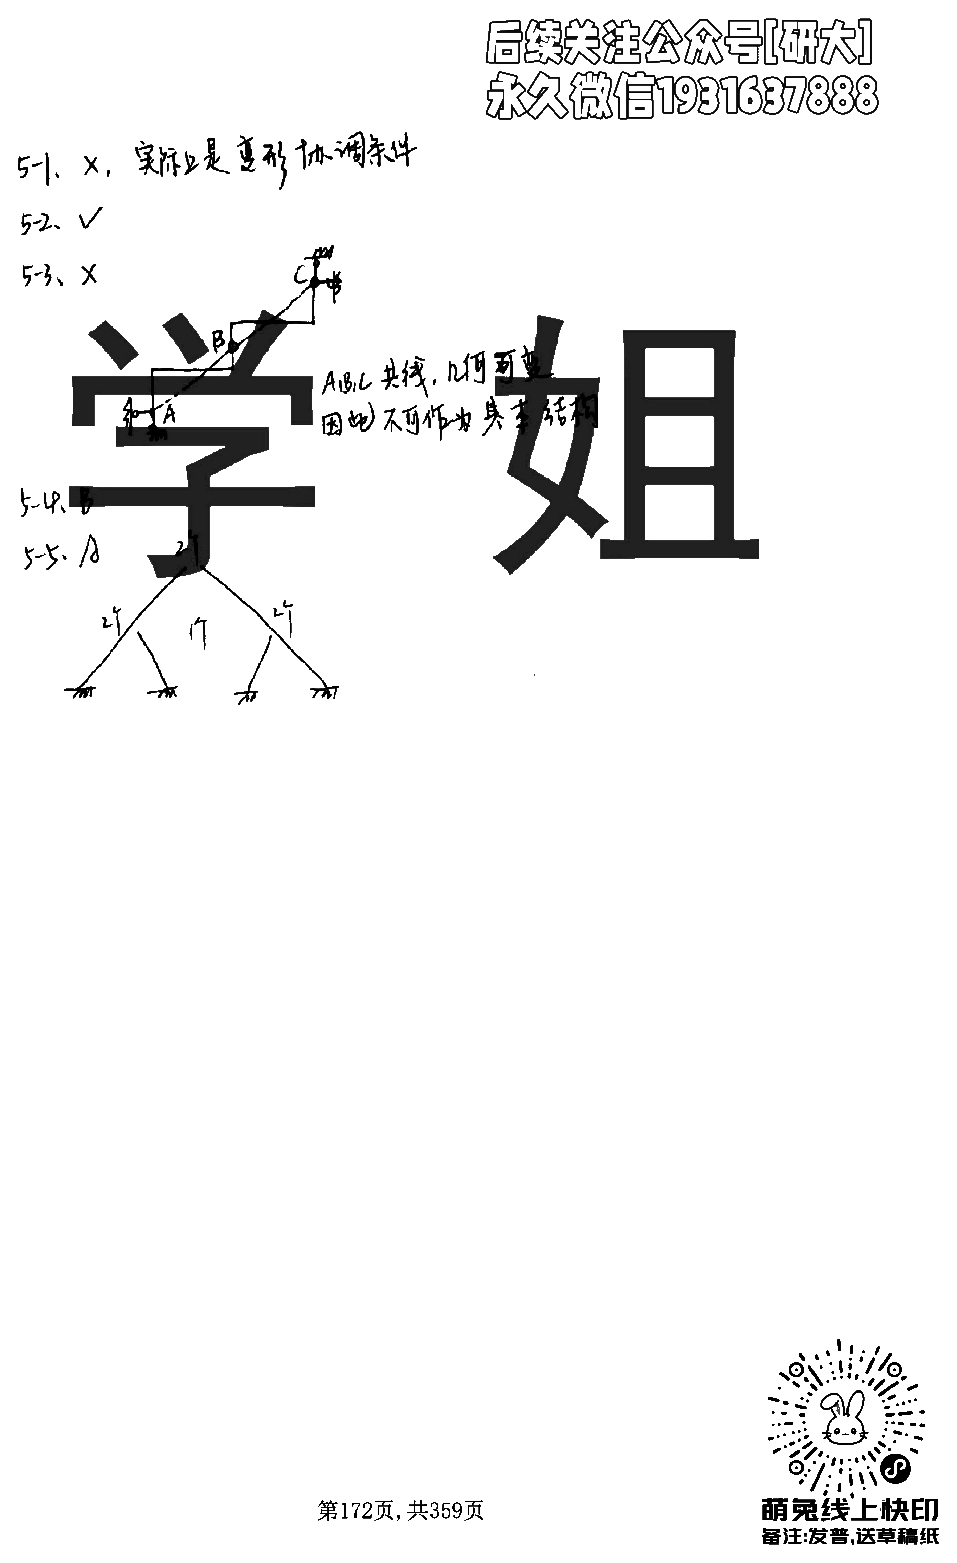
\includegraphics[width=0.96\textwidth,height=0.82\textheight,keepaspectratio]{images/c10_answer_1_p06.png}
\par\small 作业与答案（去水印版），第 6/21 页
\end{center}
\clearpage
\begin{center}
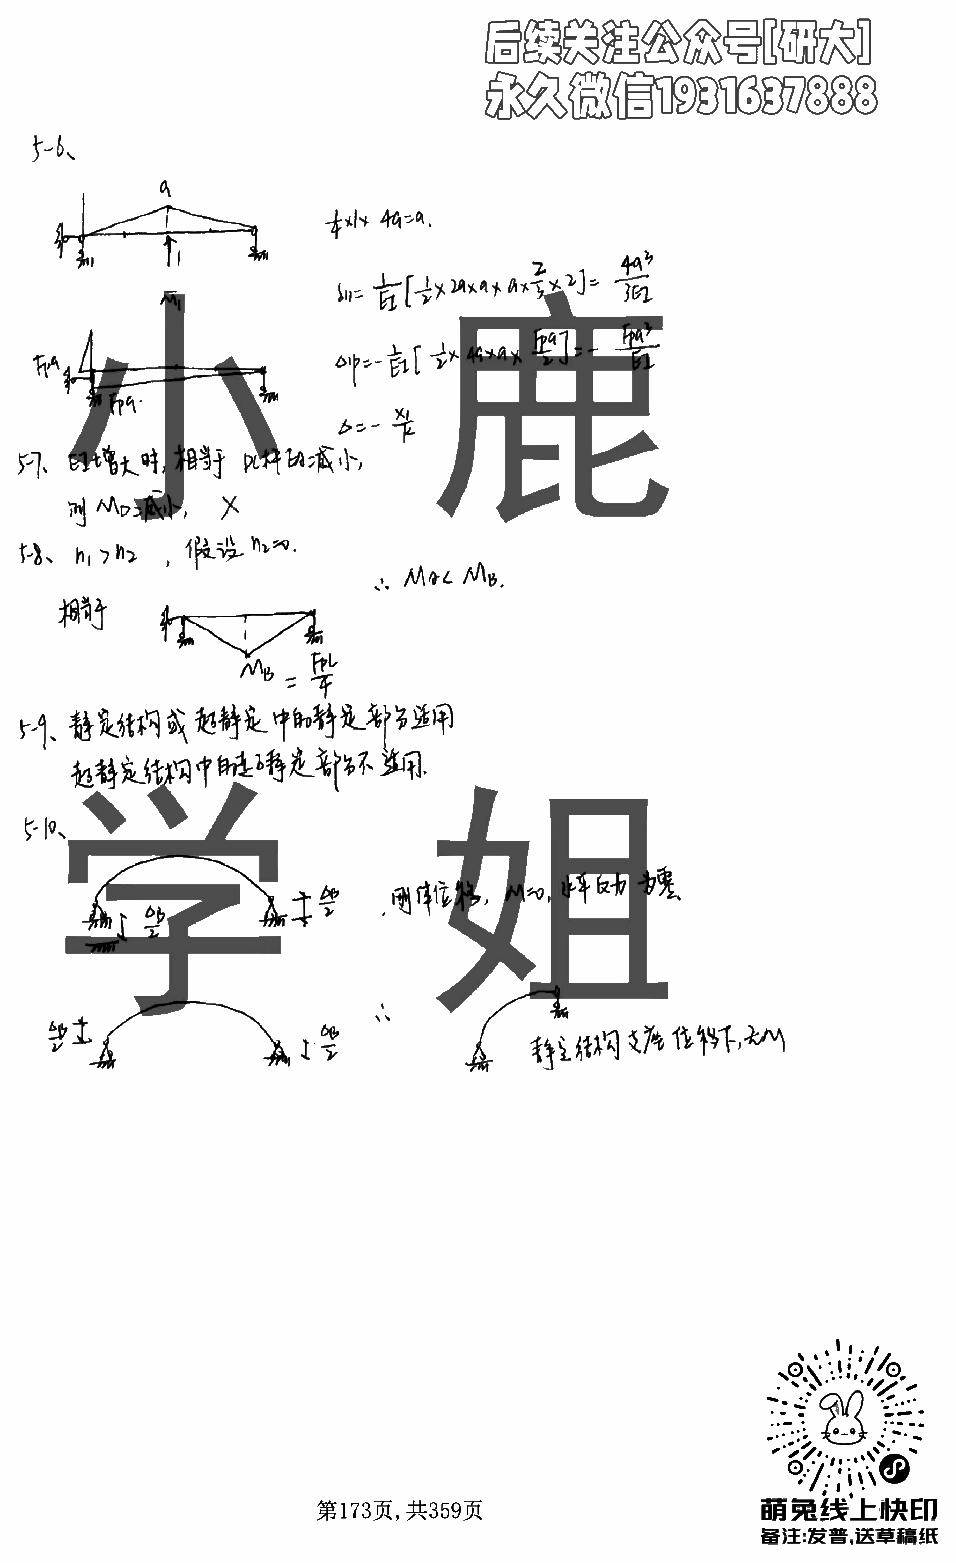
\includegraphics[width=0.96\textwidth,height=0.82\textheight,keepaspectratio]{images/c10_answer_1_p07.png}
\par\small 作业与答案（去水印版），第 7/21 页
\end{center}
\clearpage
\begin{center}
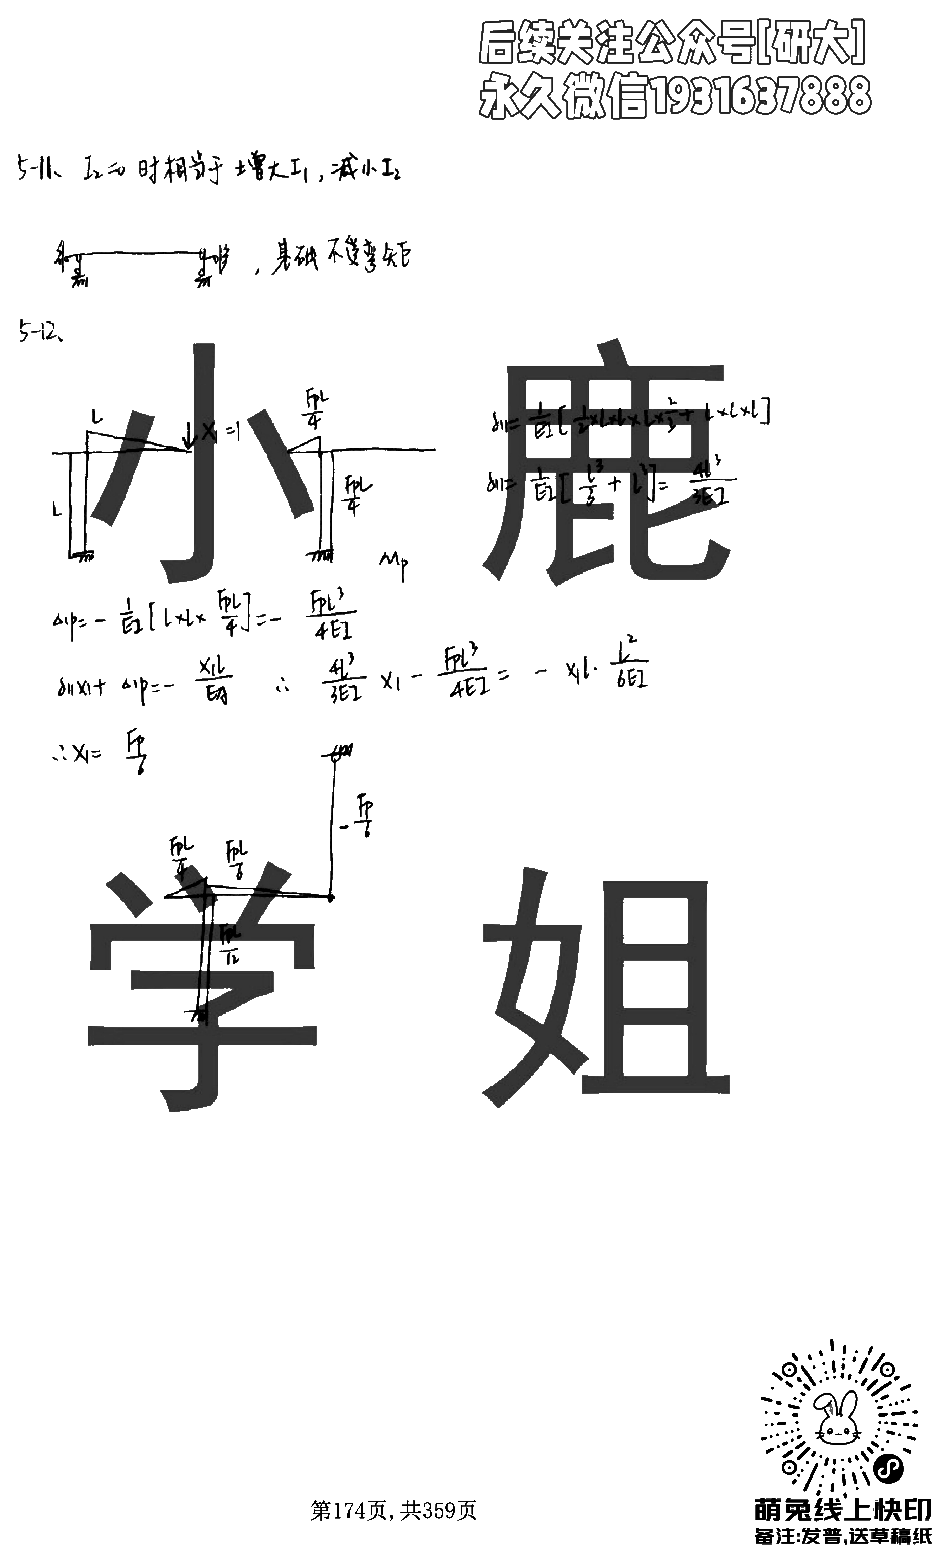
\includegraphics[width=0.96\textwidth,height=0.82\textheight,keepaspectratio]{images/c10_answer_1_p08.png}
\par\small 作业与答案（去水印版），第 8/21 页
\end{center}
\clearpage
\begin{center}
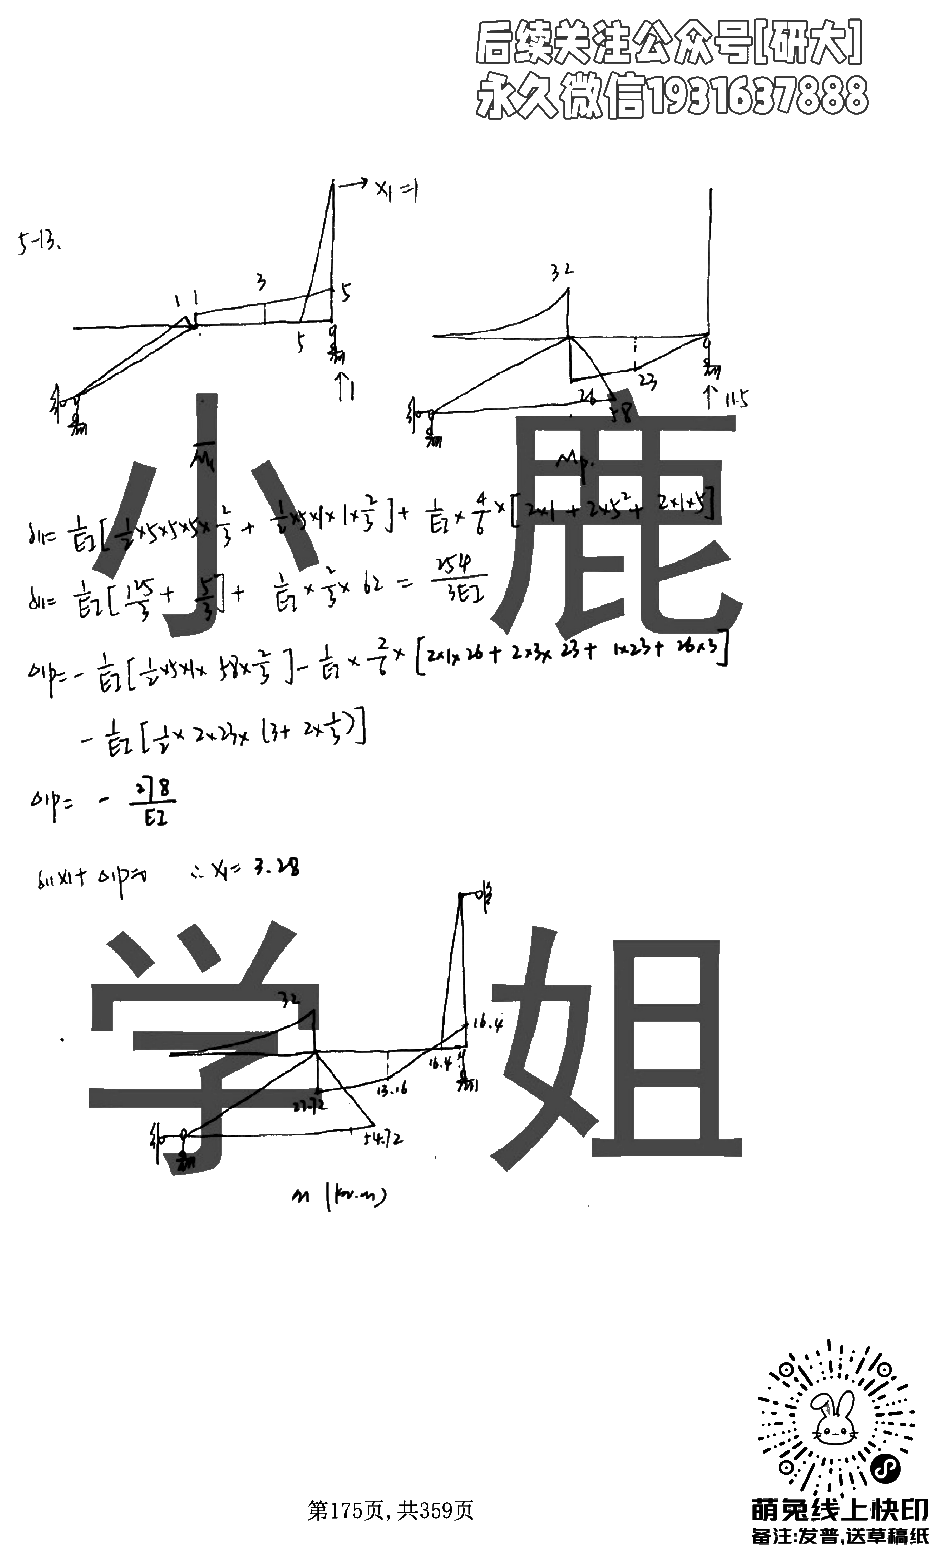
\includegraphics[width=0.96\textwidth,height=0.82\textheight,keepaspectratio]{images/c10_answer_1_p09.png}
\par\small 作业与答案（去水印版），第 9/21 页
\end{center}
\clearpage
\begin{center}
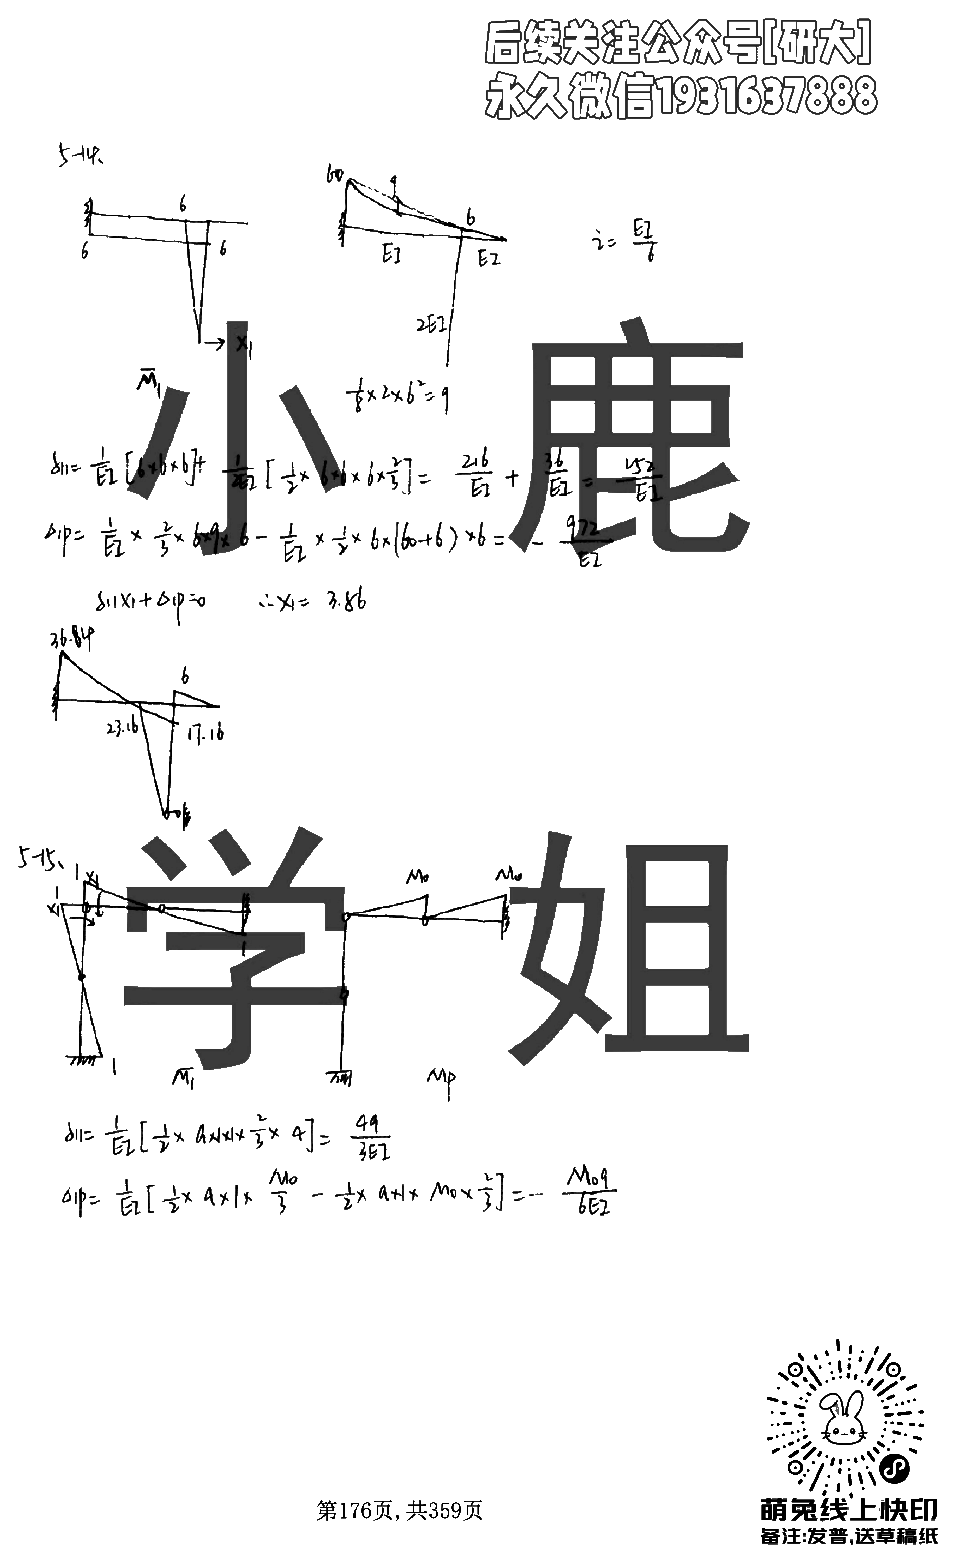
\includegraphics[width=0.96\textwidth,height=0.82\textheight,keepaspectratio]{images/c10_answer_1_p10.png}
\par\small 作业与答案（去水印版），第 10/21 页
\end{center}
\clearpage
\begin{center}
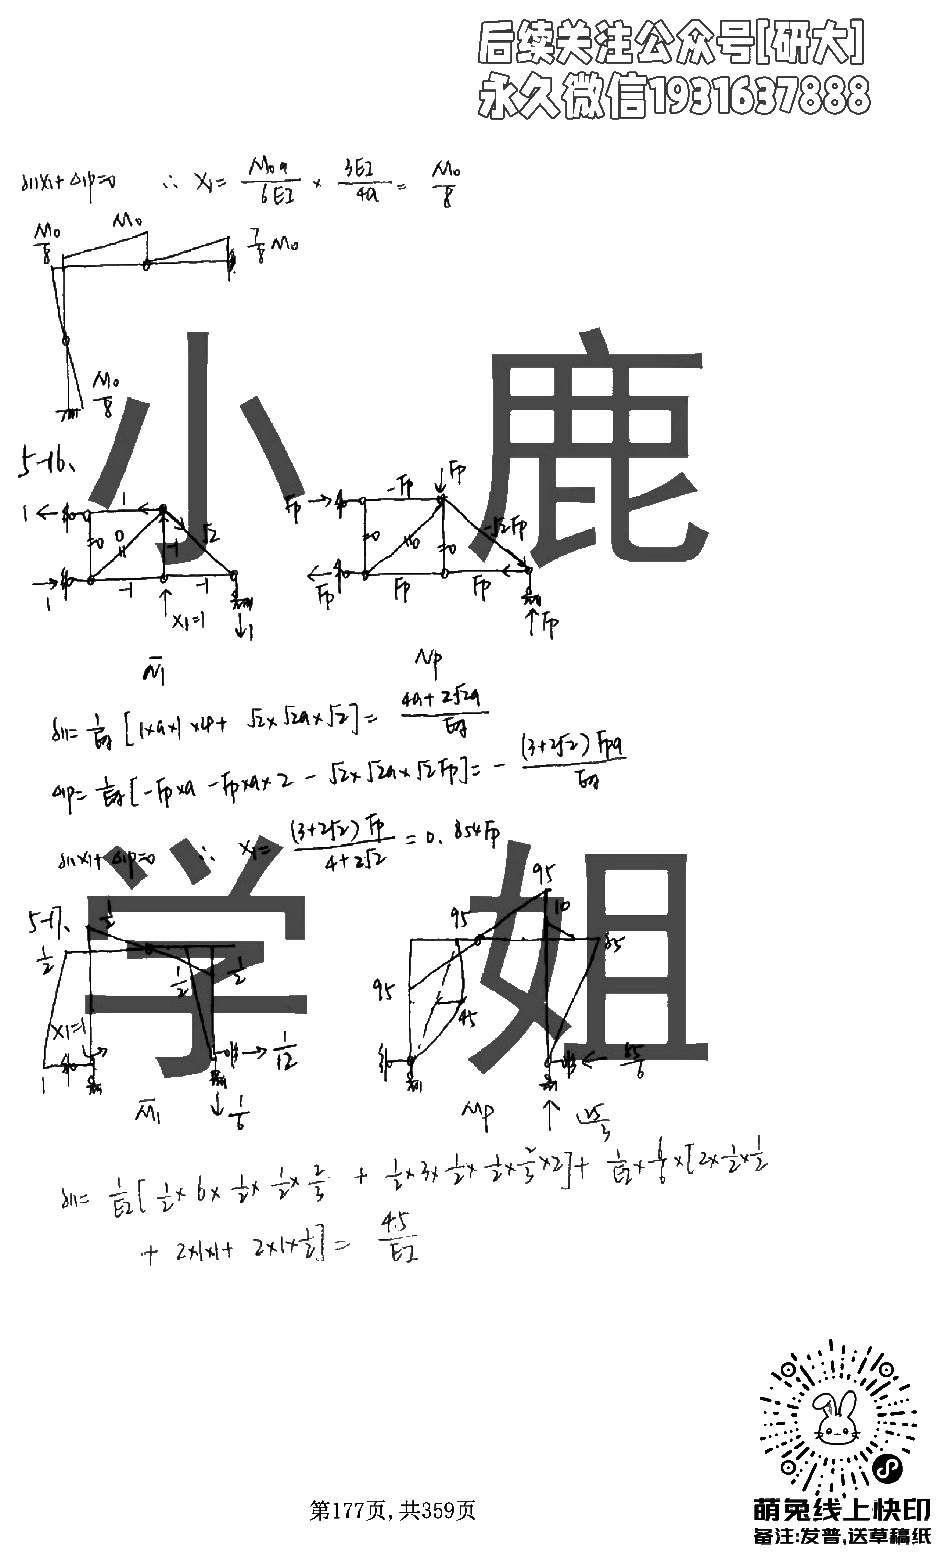
\includegraphics[width=0.96\textwidth,height=0.82\textheight,keepaspectratio]{images/c10_answer_1_p11.png}
\par\small 作业与答案（去水印版），第 11/21 页
\end{center}
\clearpage
\begin{center}
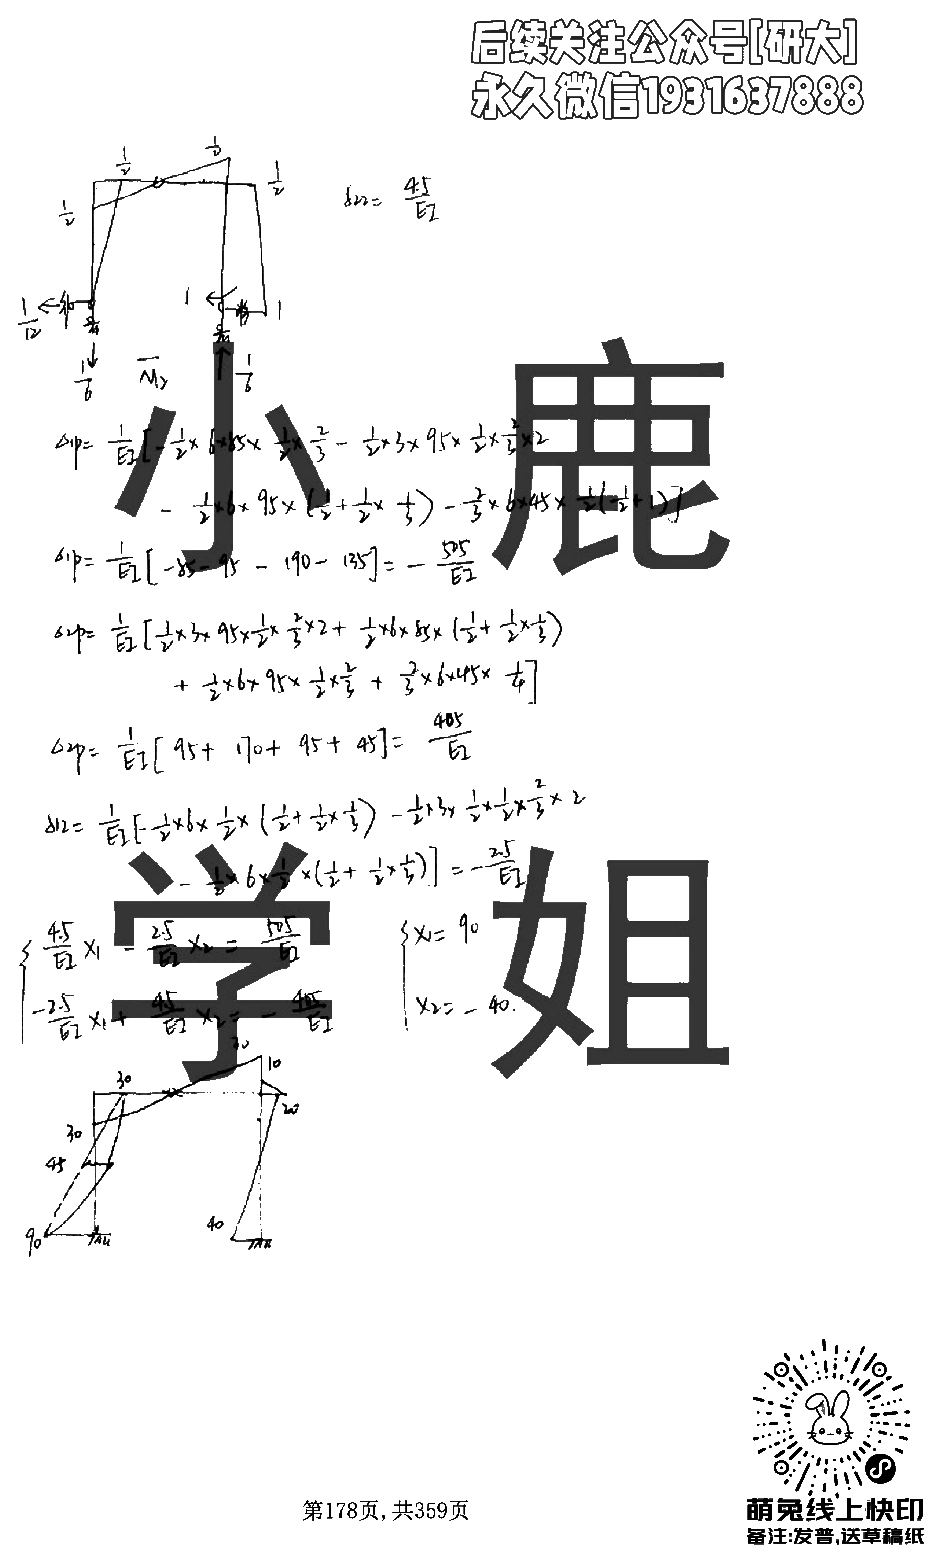
\includegraphics[width=0.96\textwidth,height=0.82\textheight,keepaspectratio]{images/c10_answer_1_p12.png}
\par\small 作业与答案（去水印版），第 12/21 页
\end{center}
\clearpage
\begin{center}
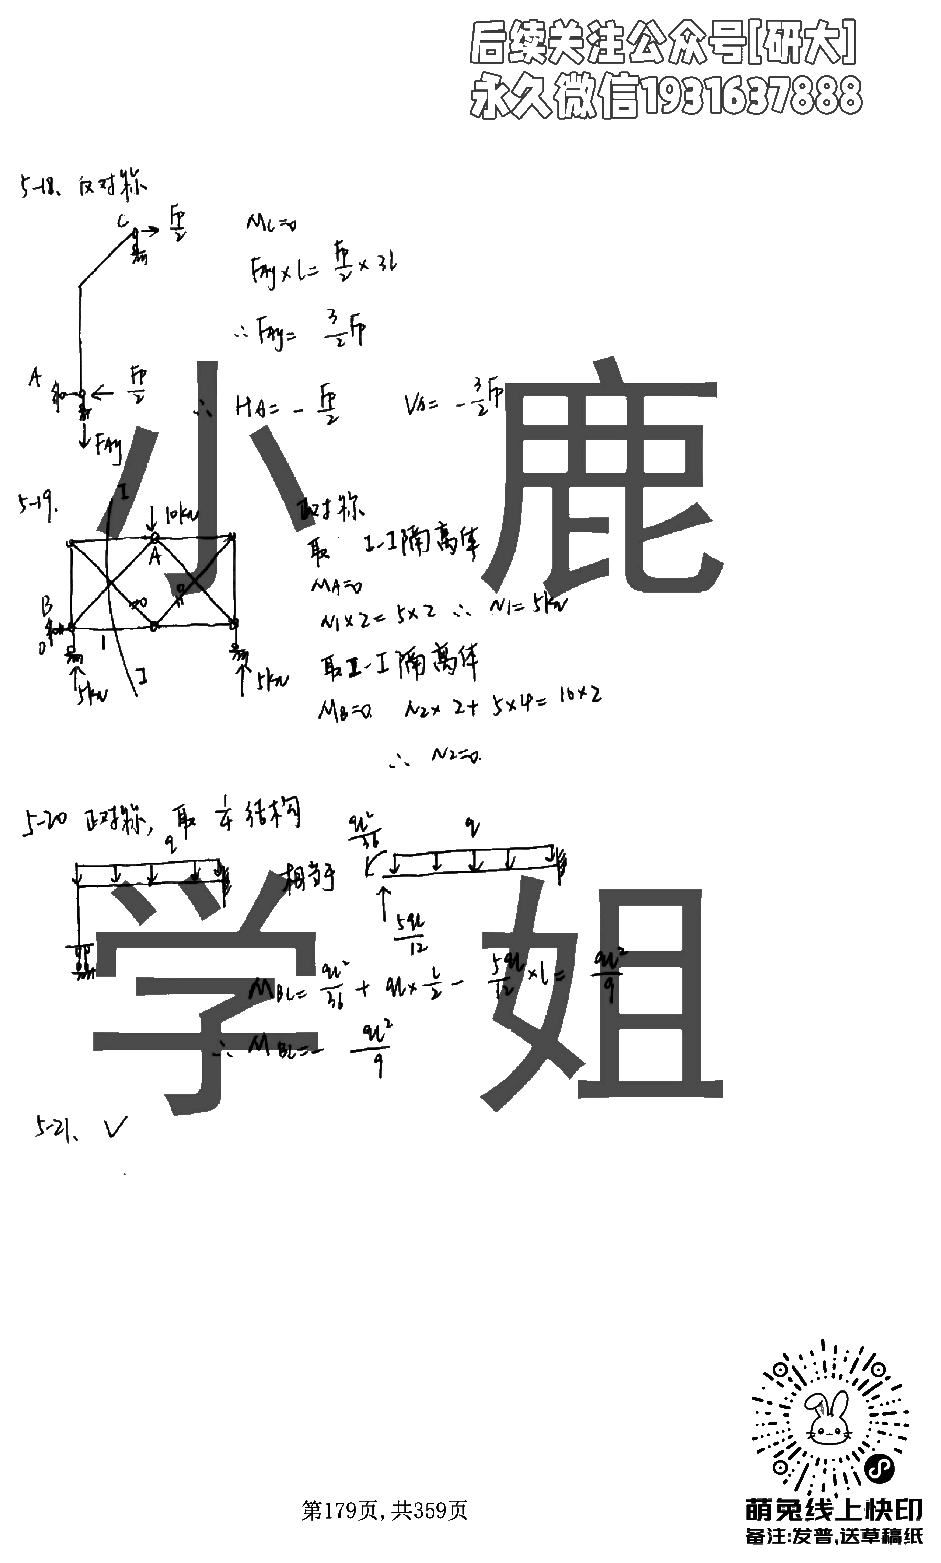
\includegraphics[width=0.96\textwidth,height=0.82\textheight,keepaspectratio]{images/c10_answer_1_p13.png}
\par\small 作业与答案（去水印版），第 13/21 页
\end{center}
\clearpage
\begin{center}
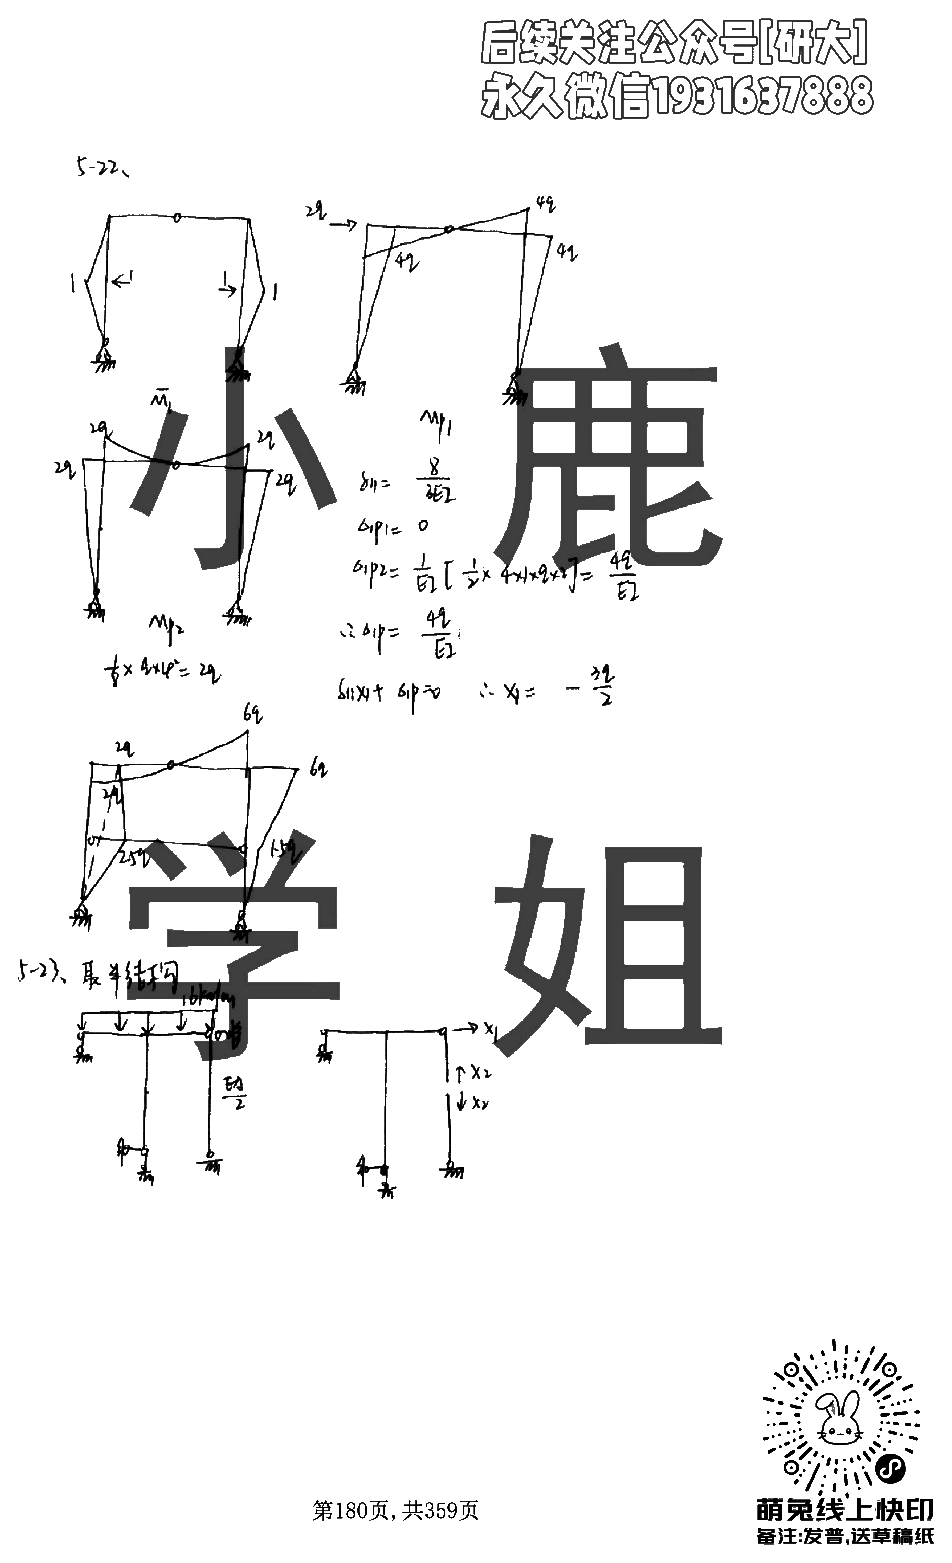
\includegraphics[width=0.96\textwidth,height=0.82\textheight,keepaspectratio]{images/c10_answer_1_p14.png}
\par\small 作业与答案（去水印版），第 14/21 页
\end{center}
\clearpage
\begin{center}
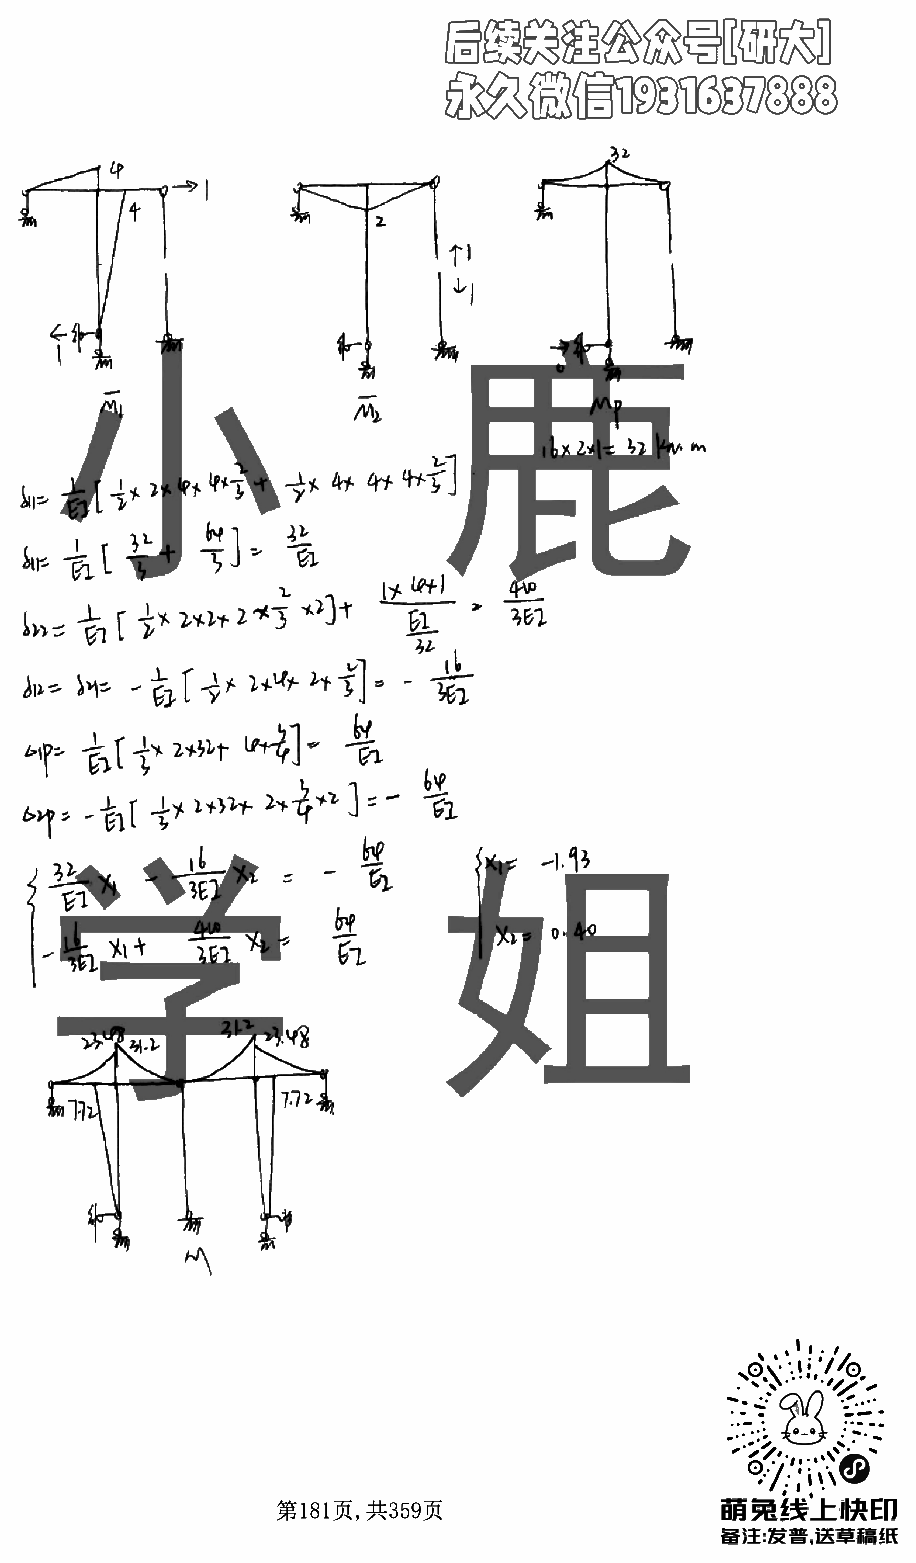
\includegraphics[width=0.96\textwidth,height=0.82\textheight,keepaspectratio]{images/c10_answer_1_p15.png}
\par\small 作业与答案（去水印版），第 15/21 页
\end{center}
\clearpage
\begin{center}
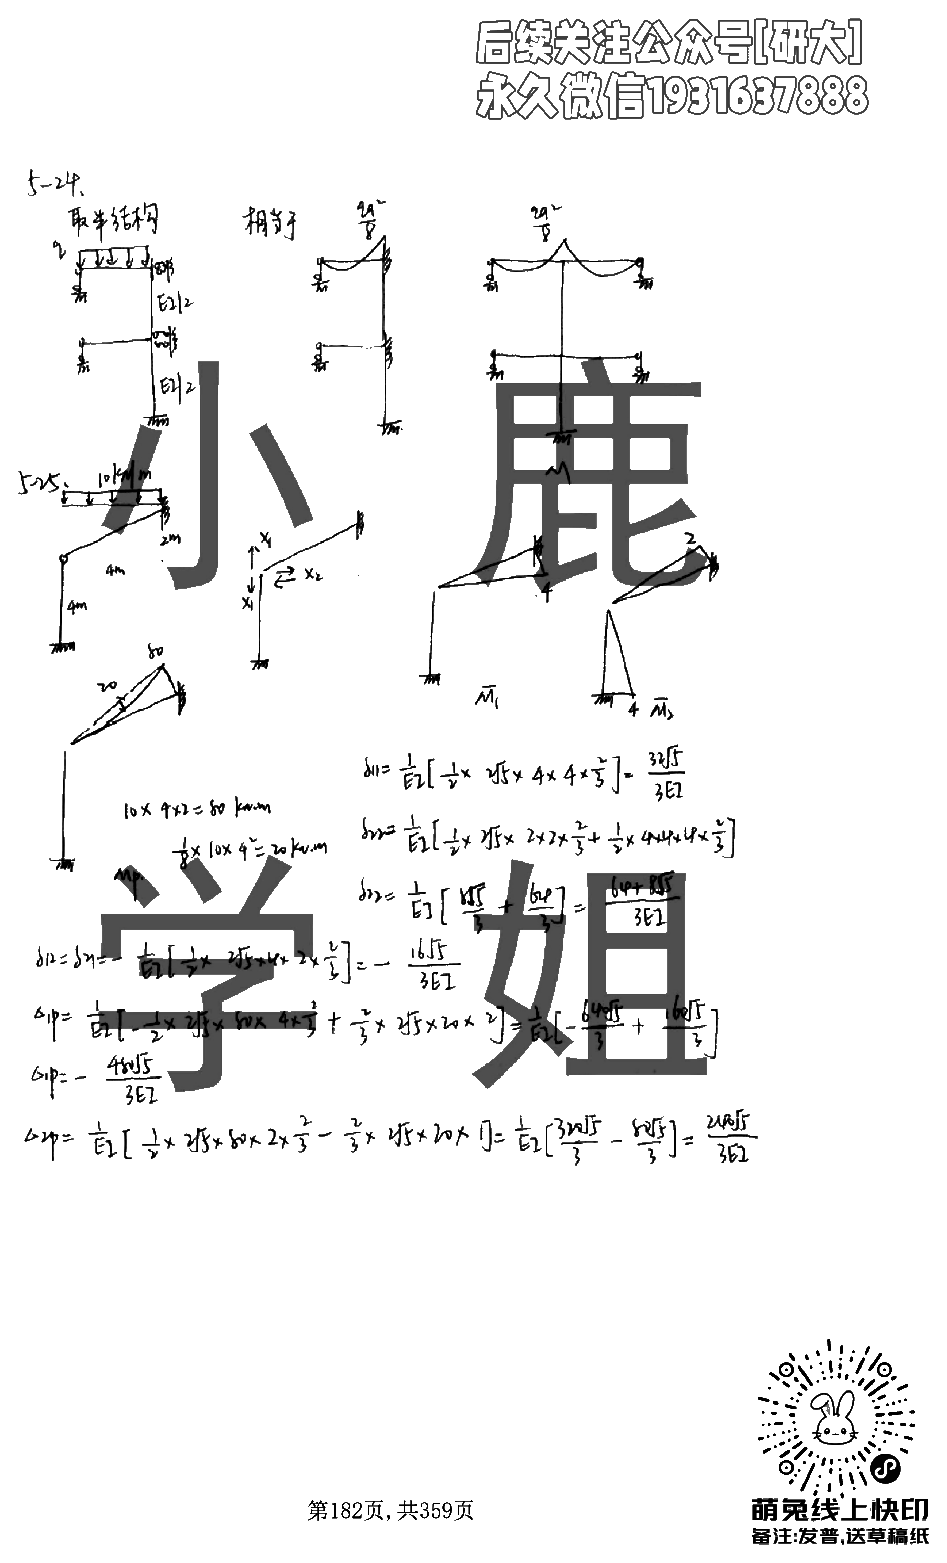
\includegraphics[width=0.96\textwidth,height=0.82\textheight,keepaspectratio]{images/c10_answer_1_p16.png}
\par\small 作业与答案（去水印版），第 16/21 页
\end{center}
\clearpage
\begin{center}
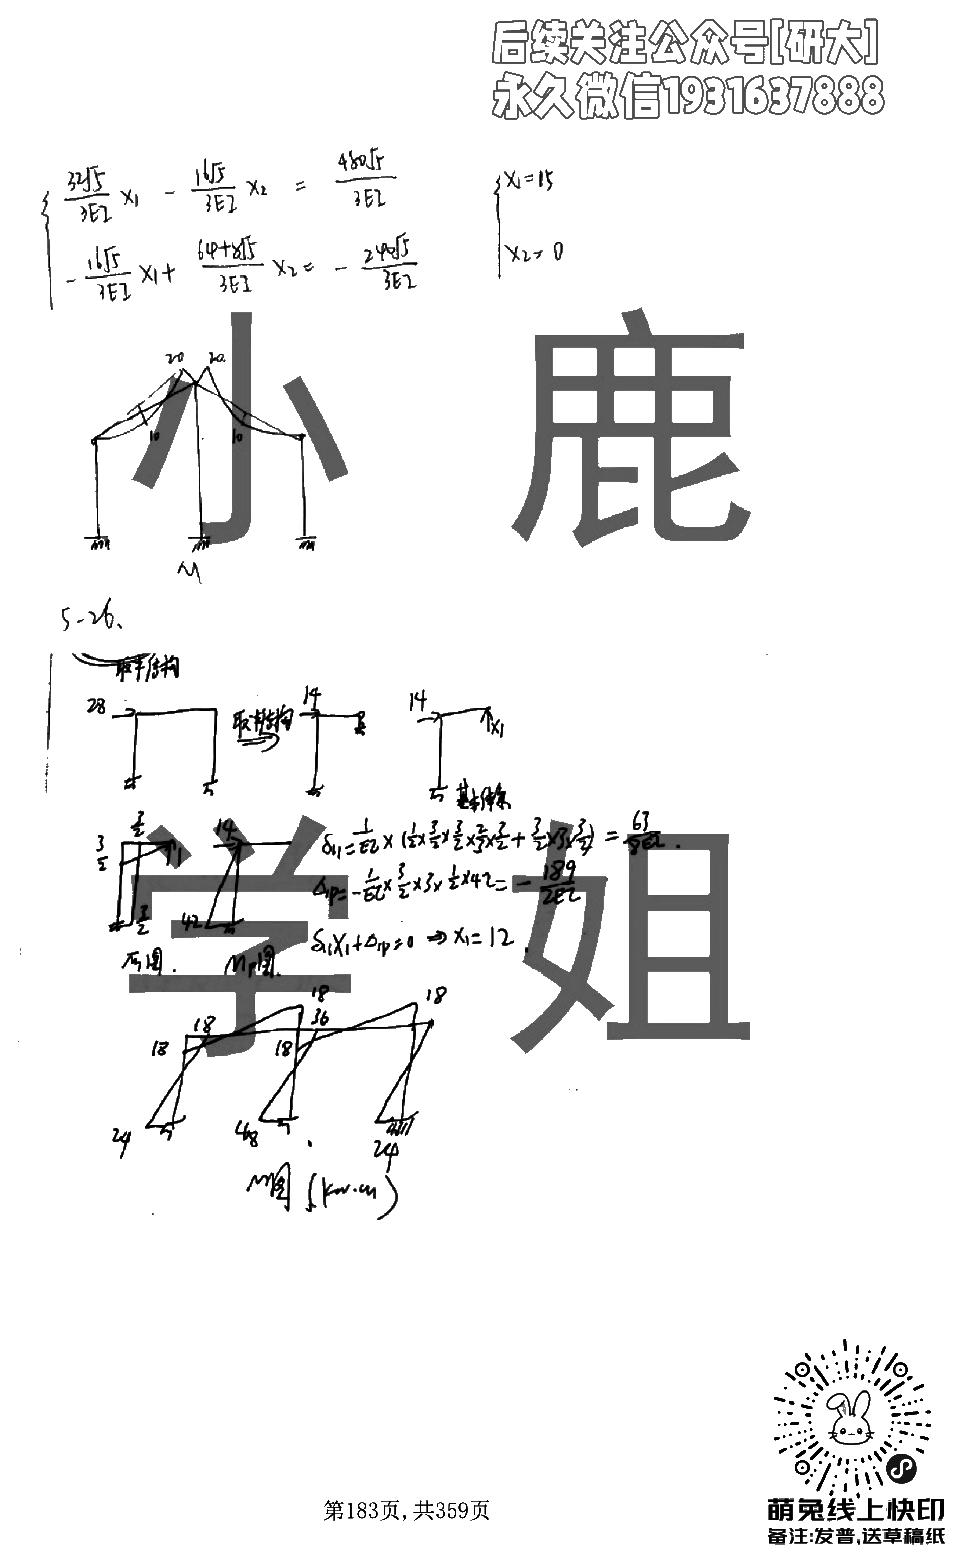
\includegraphics[width=0.96\textwidth,height=0.82\textheight,keepaspectratio]{images/c10_answer_1_p17.png}
\par\small 作业与答案（去水印版），第 17/21 页
\end{center}
\clearpage
\begin{center}
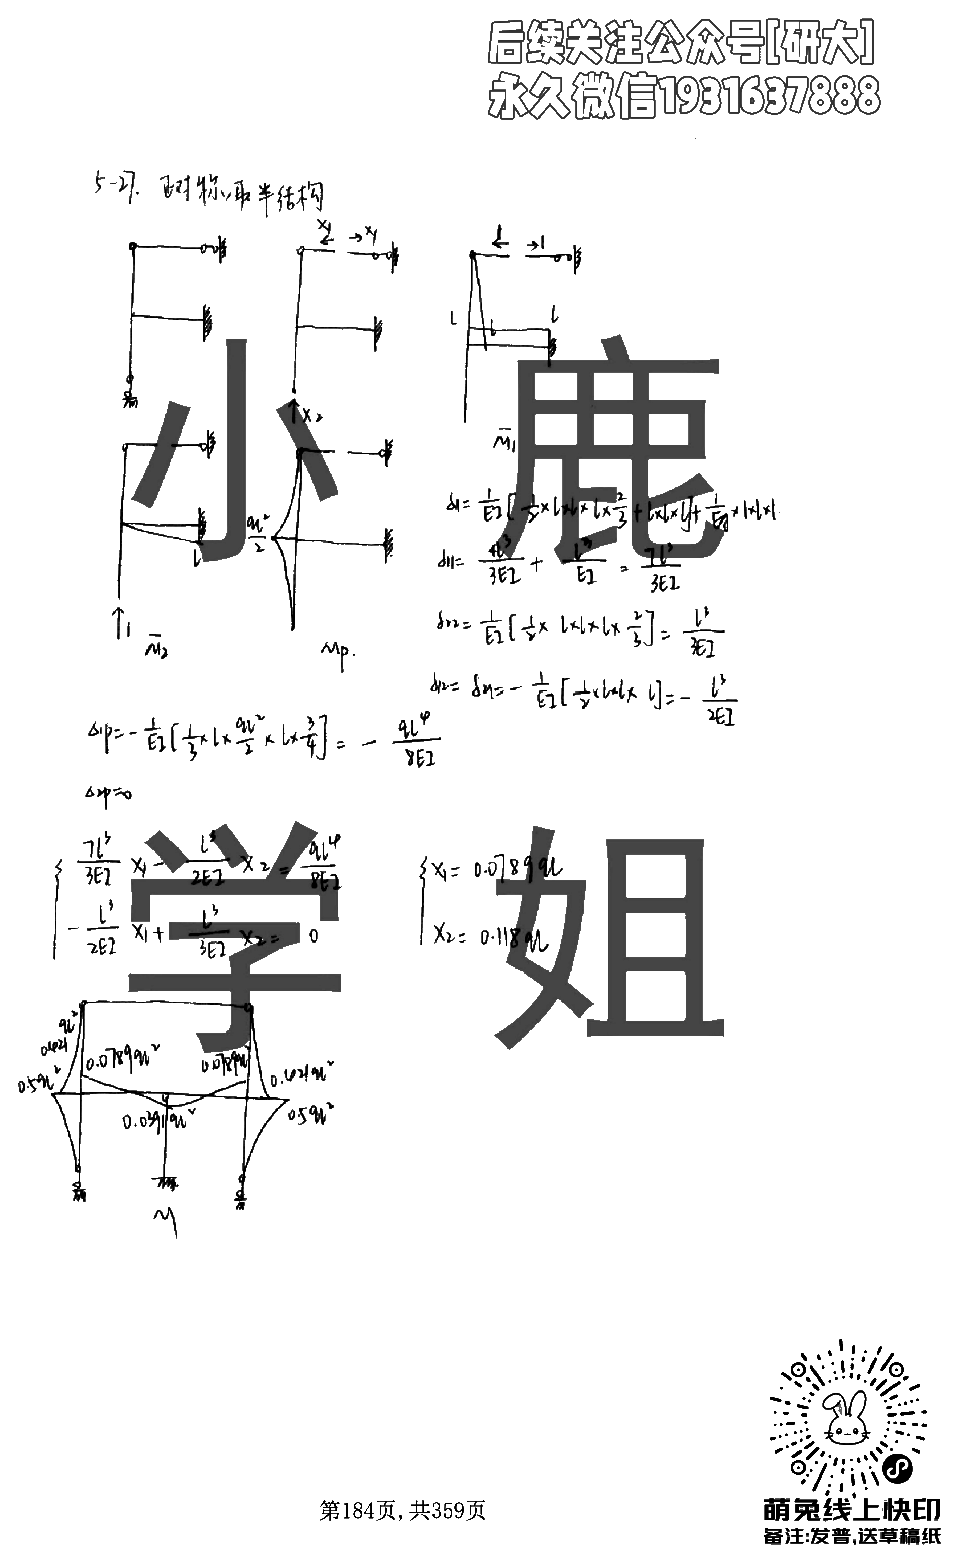
\includegraphics[width=0.96\textwidth,height=0.82\textheight,keepaspectratio]{images/c10_answer_1_p18.png}
\par\small 作业与答案（去水印版），第 18/21 页
\end{center}
\clearpage
\begin{center}
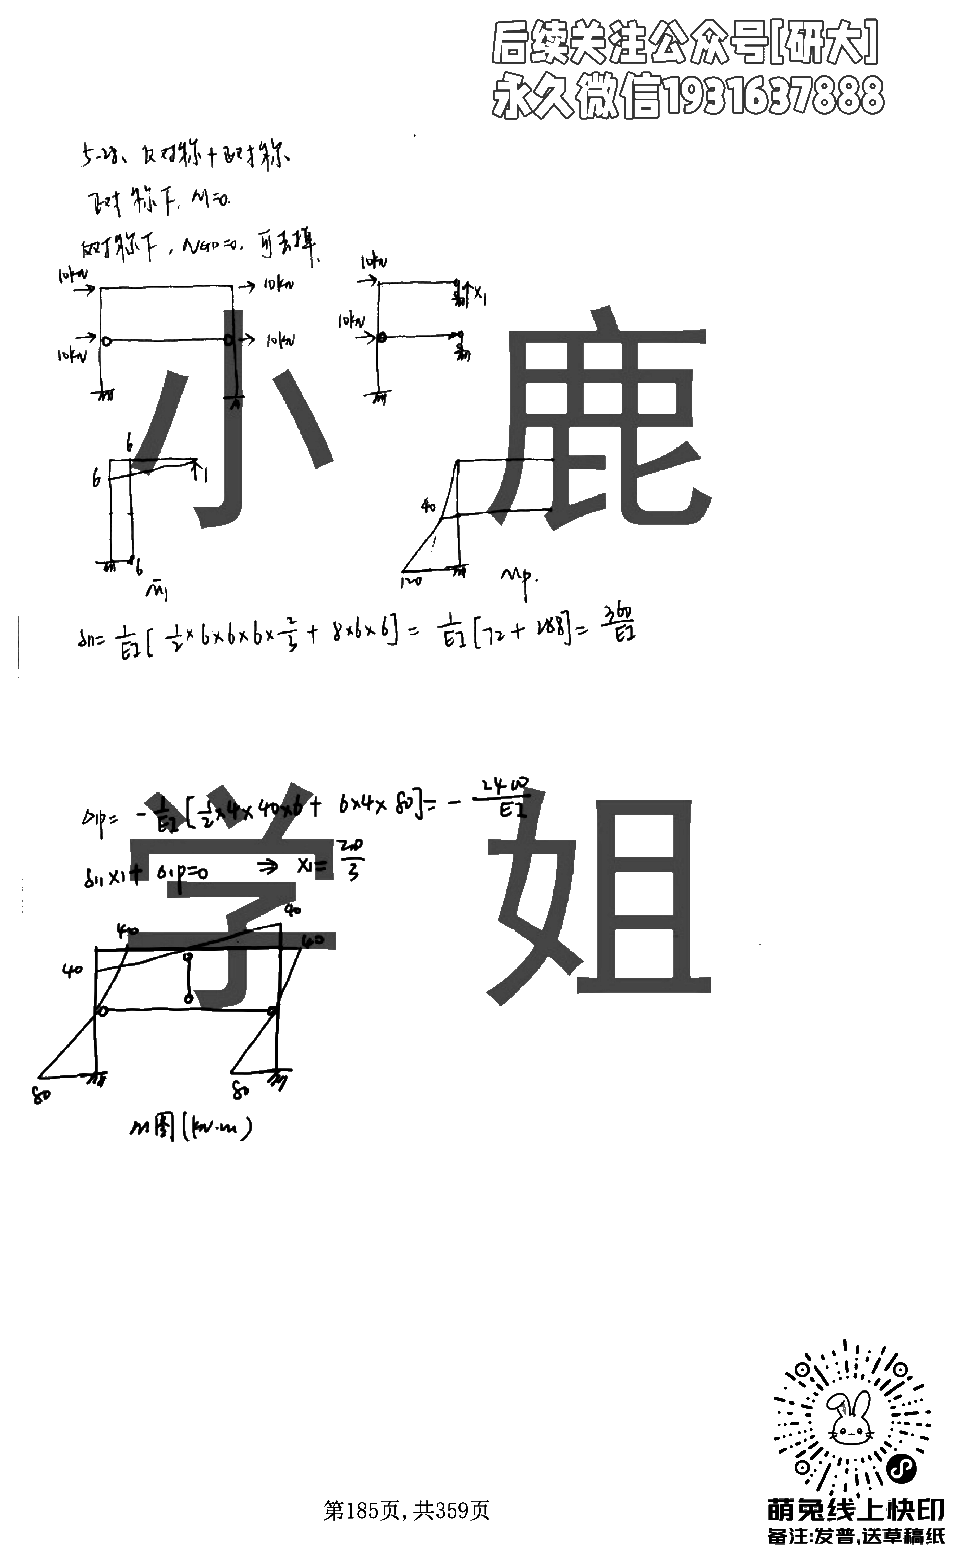
\includegraphics[width=0.96\textwidth,height=0.82\textheight,keepaspectratio]{images/c10_answer_1_p19.png}
\par\small 作业与答案（去水印版），第 19/21 页
\end{center}
\clearpage
\begin{center}
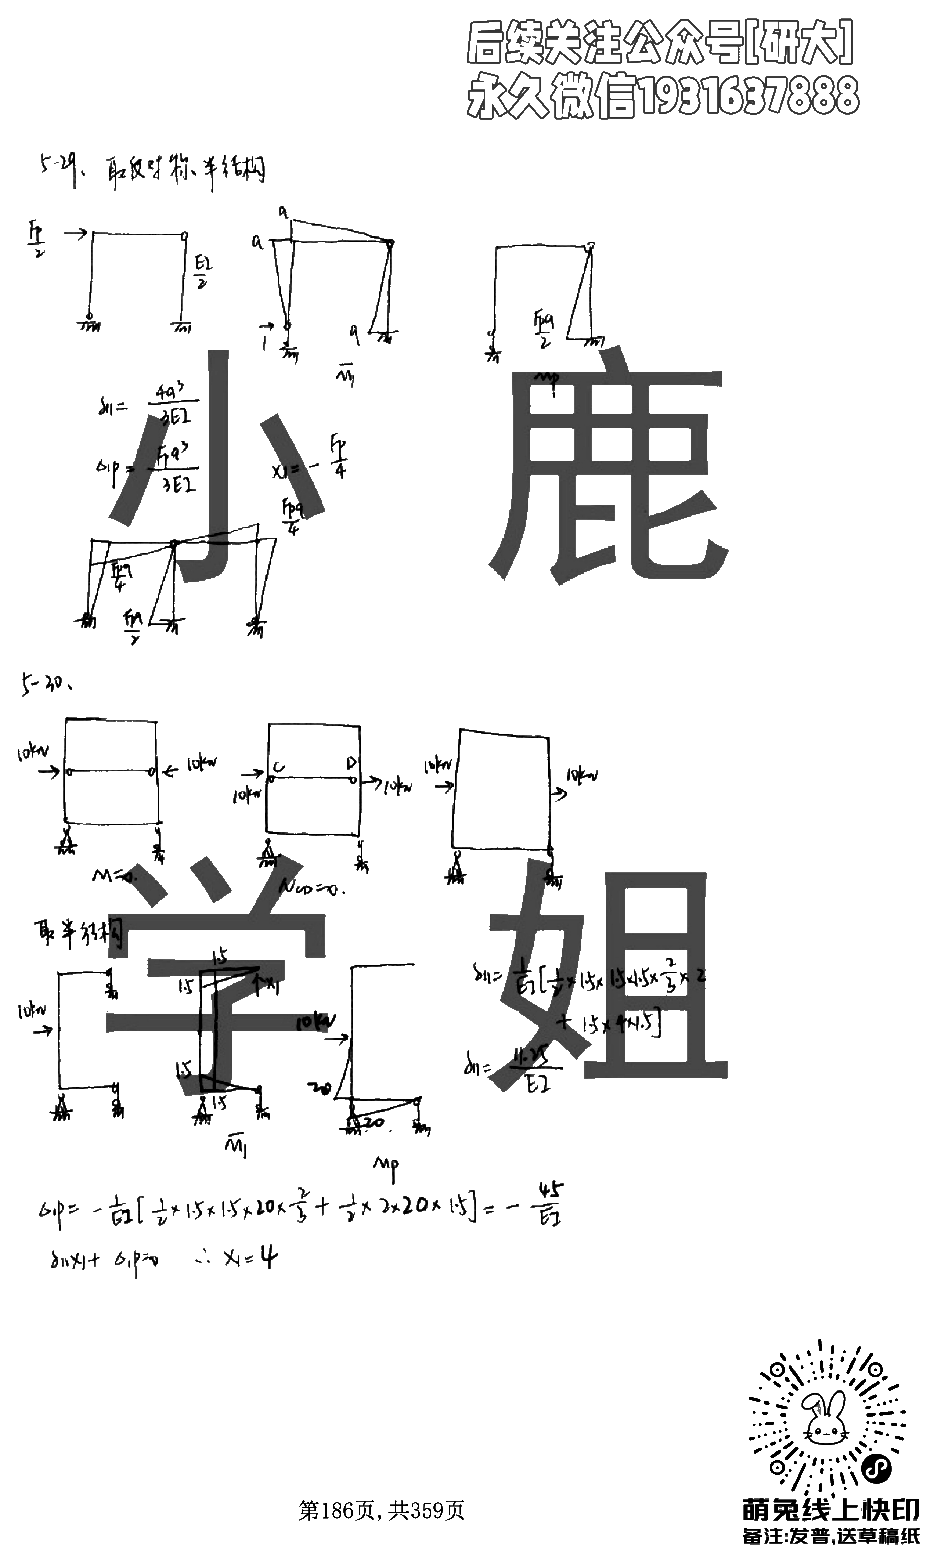
\includegraphics[width=0.96\textwidth,height=0.82\textheight,keepaspectratio]{images/c10_answer_1_p20.png}
\par\small 作业与答案（去水印版），第 20/21 页
\end{center}
\clearpage
\begin{center}
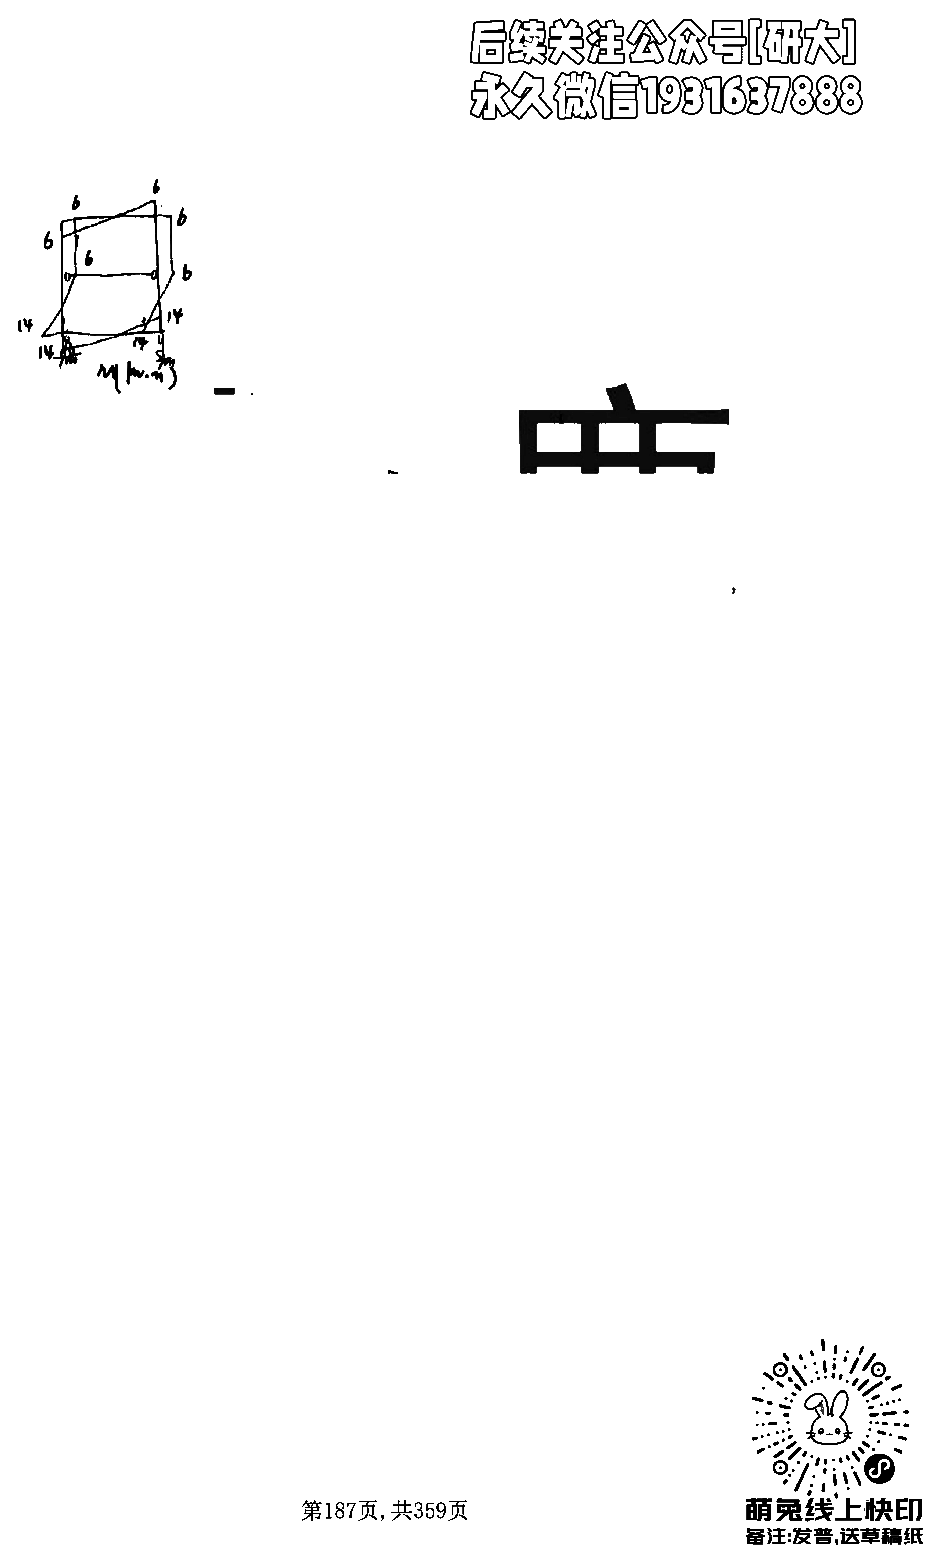
\includegraphics[width=0.96\textwidth,height=0.82\textheight,keepaspectratio]{images/c10_answer_1_p21.png}
\par\small 作业与答案（去水印版），第 21/21 页
\end{center}
\clearpage
\section{讲解笔记（去水印版）}
\begin{center}
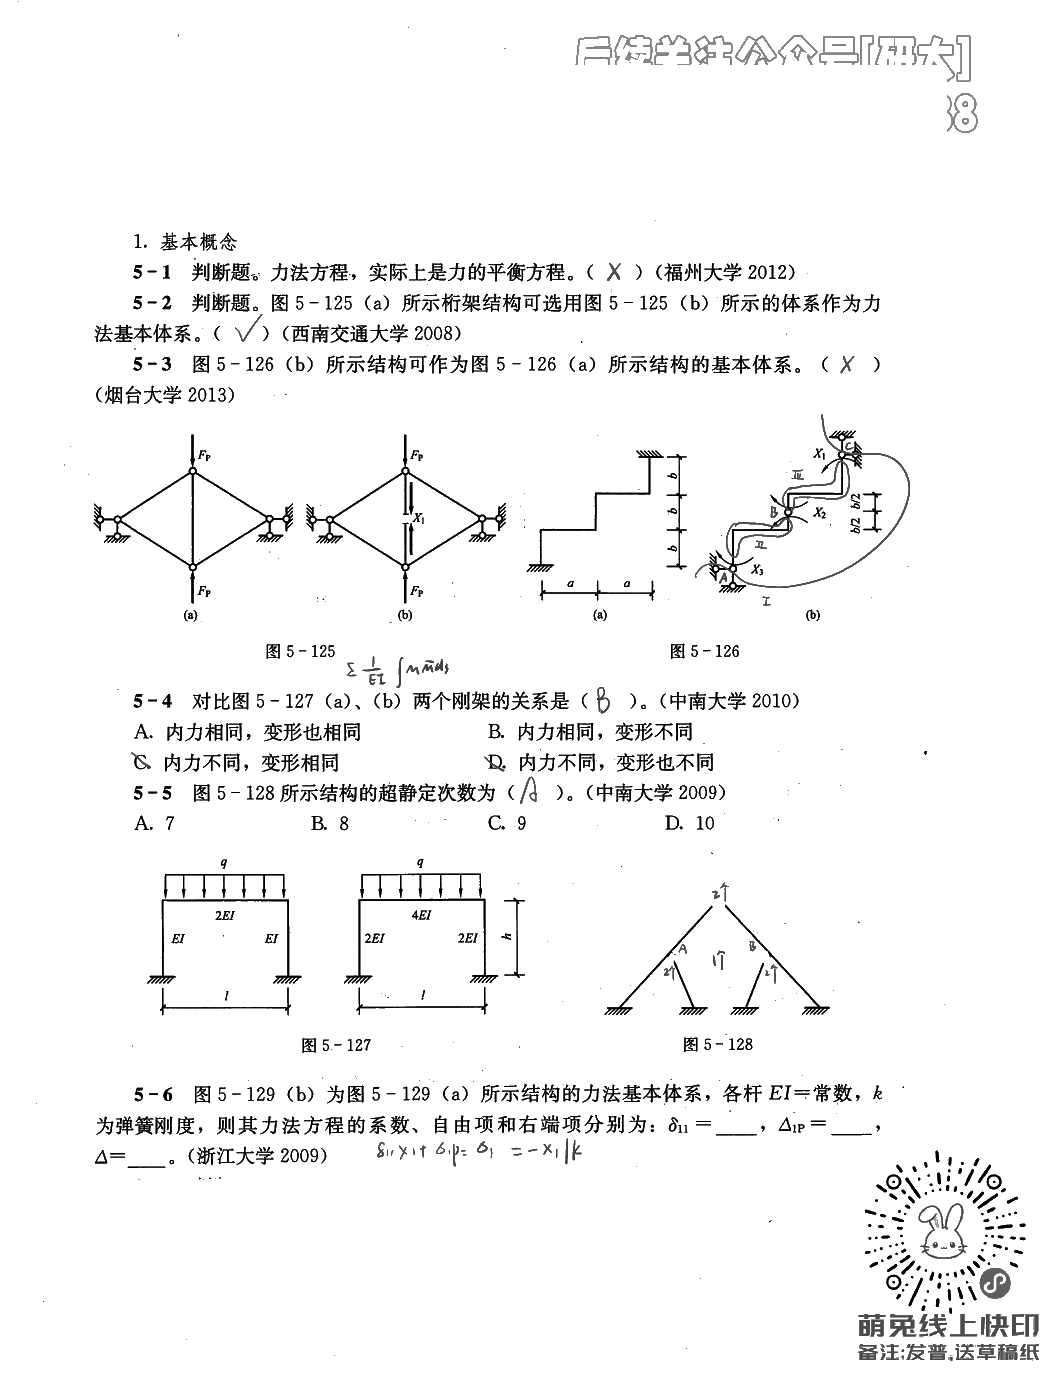
\includegraphics[width=0.96\textwidth,height=0.82\textheight,keepaspectratio]{images/c10_note_p01.png}
\par\small 讲解笔记（去水印版），第 1/21 页
\end{center}
\clearpage
\begin{center}
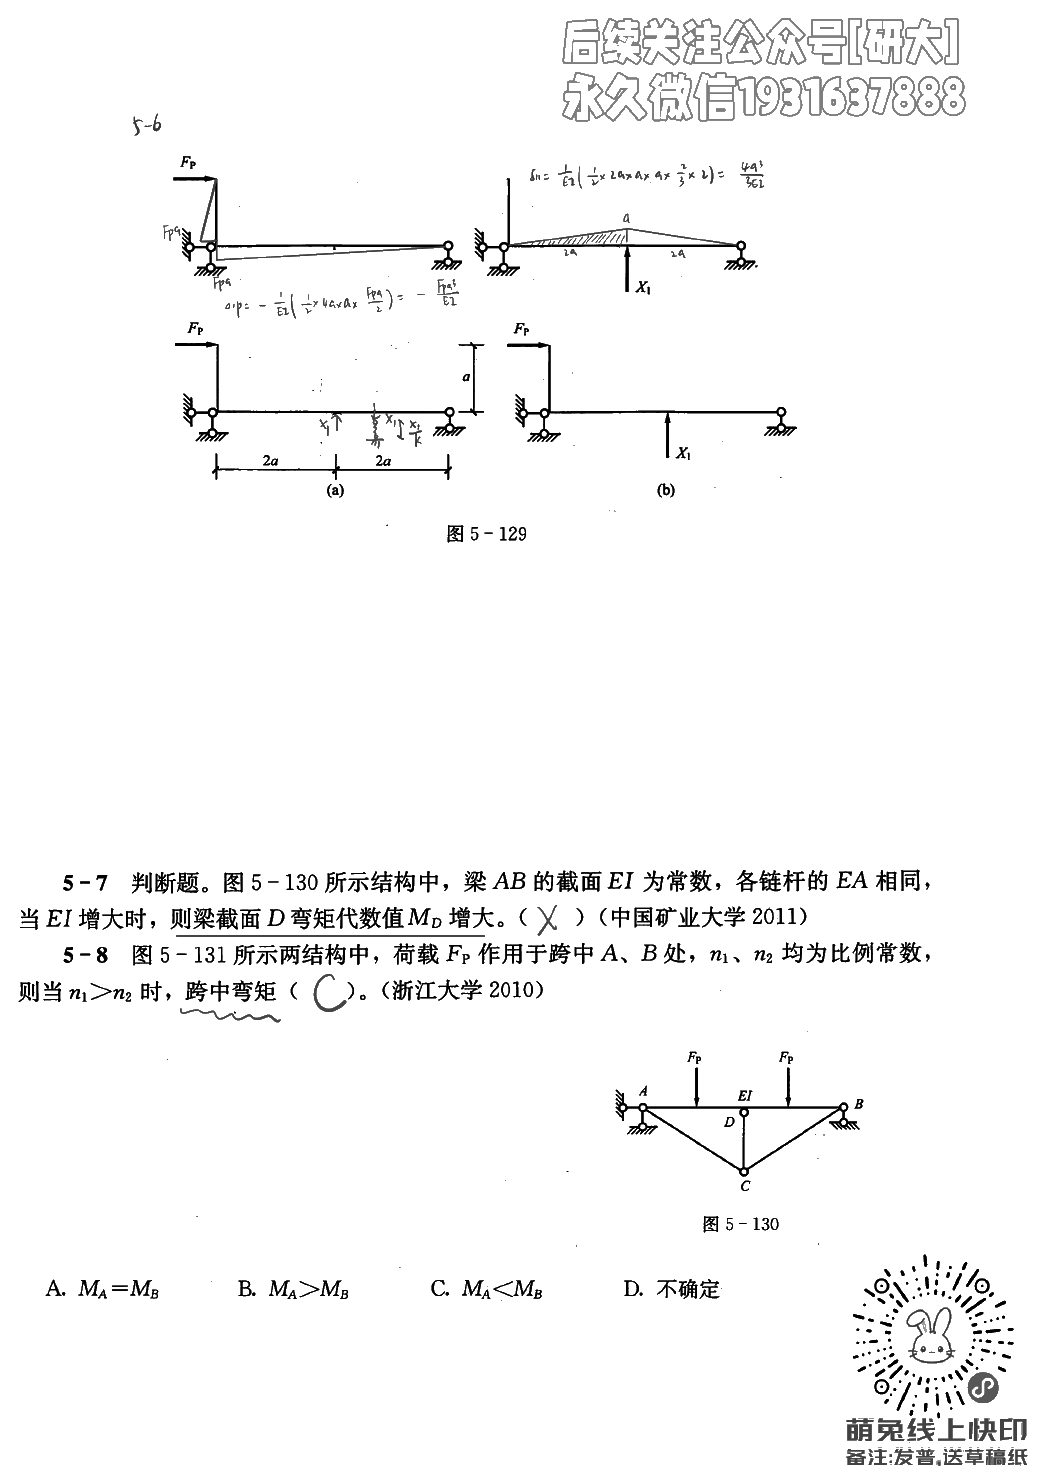
\includegraphics[width=0.96\textwidth,height=0.82\textheight,keepaspectratio]{images/c10_note_p02.png}
\par\small 讲解笔记（去水印版），第 2/21 页
\end{center}
\clearpage
\begin{center}
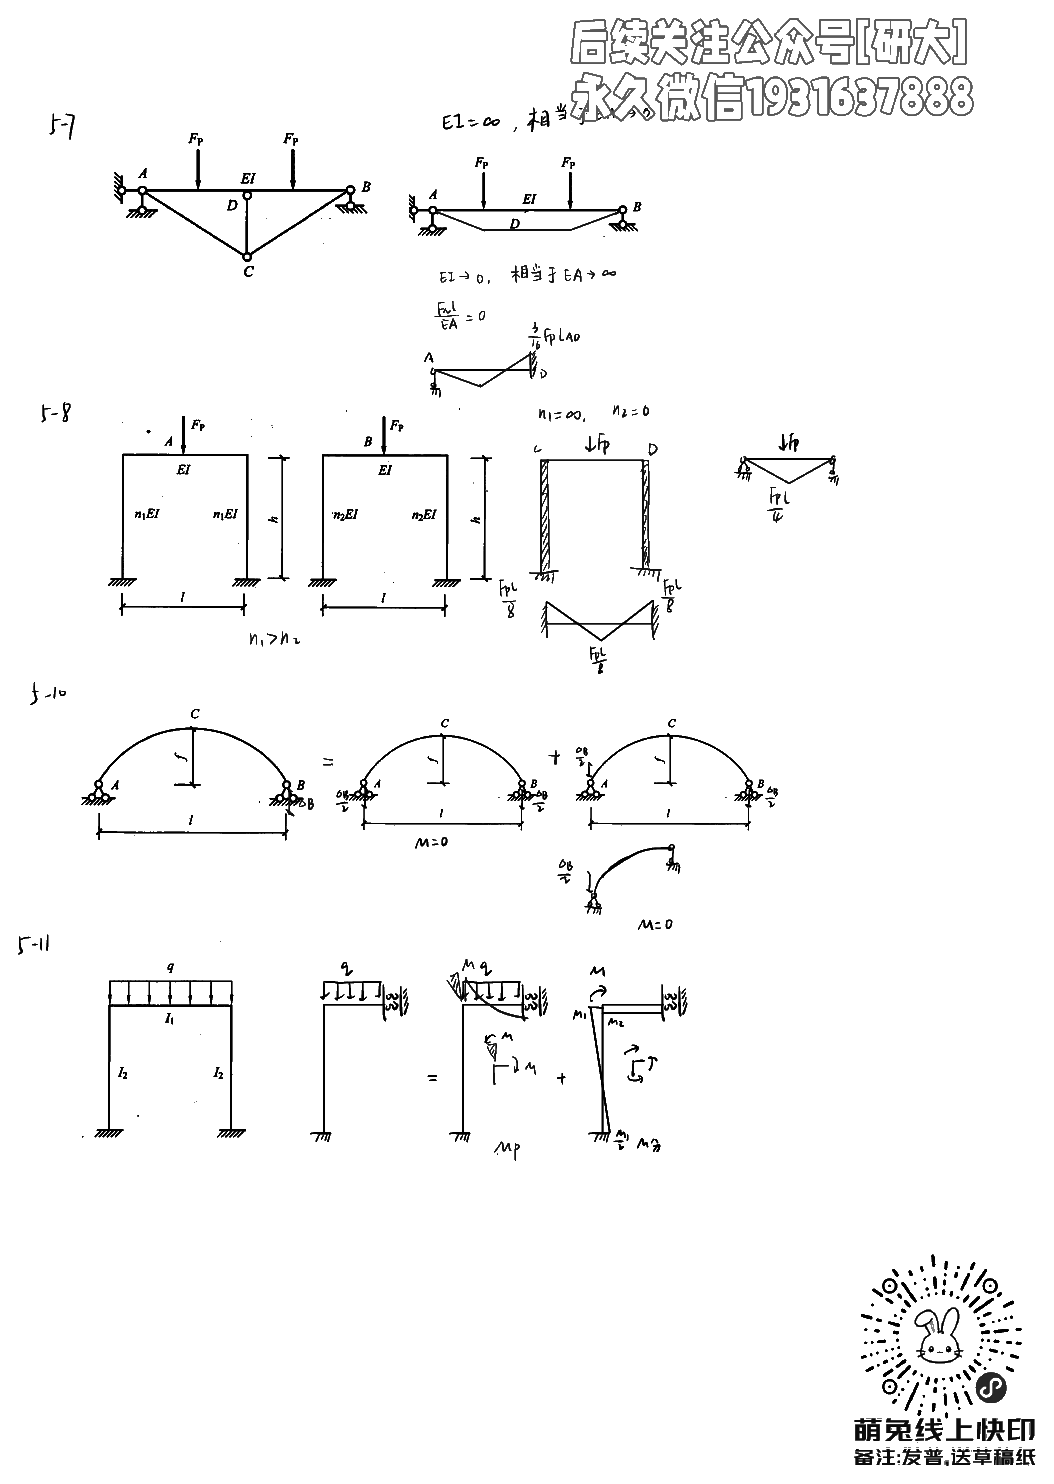
\includegraphics[width=0.96\textwidth,height=0.82\textheight,keepaspectratio]{images/c10_note_p03.png}
\par\small 讲解笔记（去水印版），第 3/21 页
\end{center}
\clearpage
\begin{center}
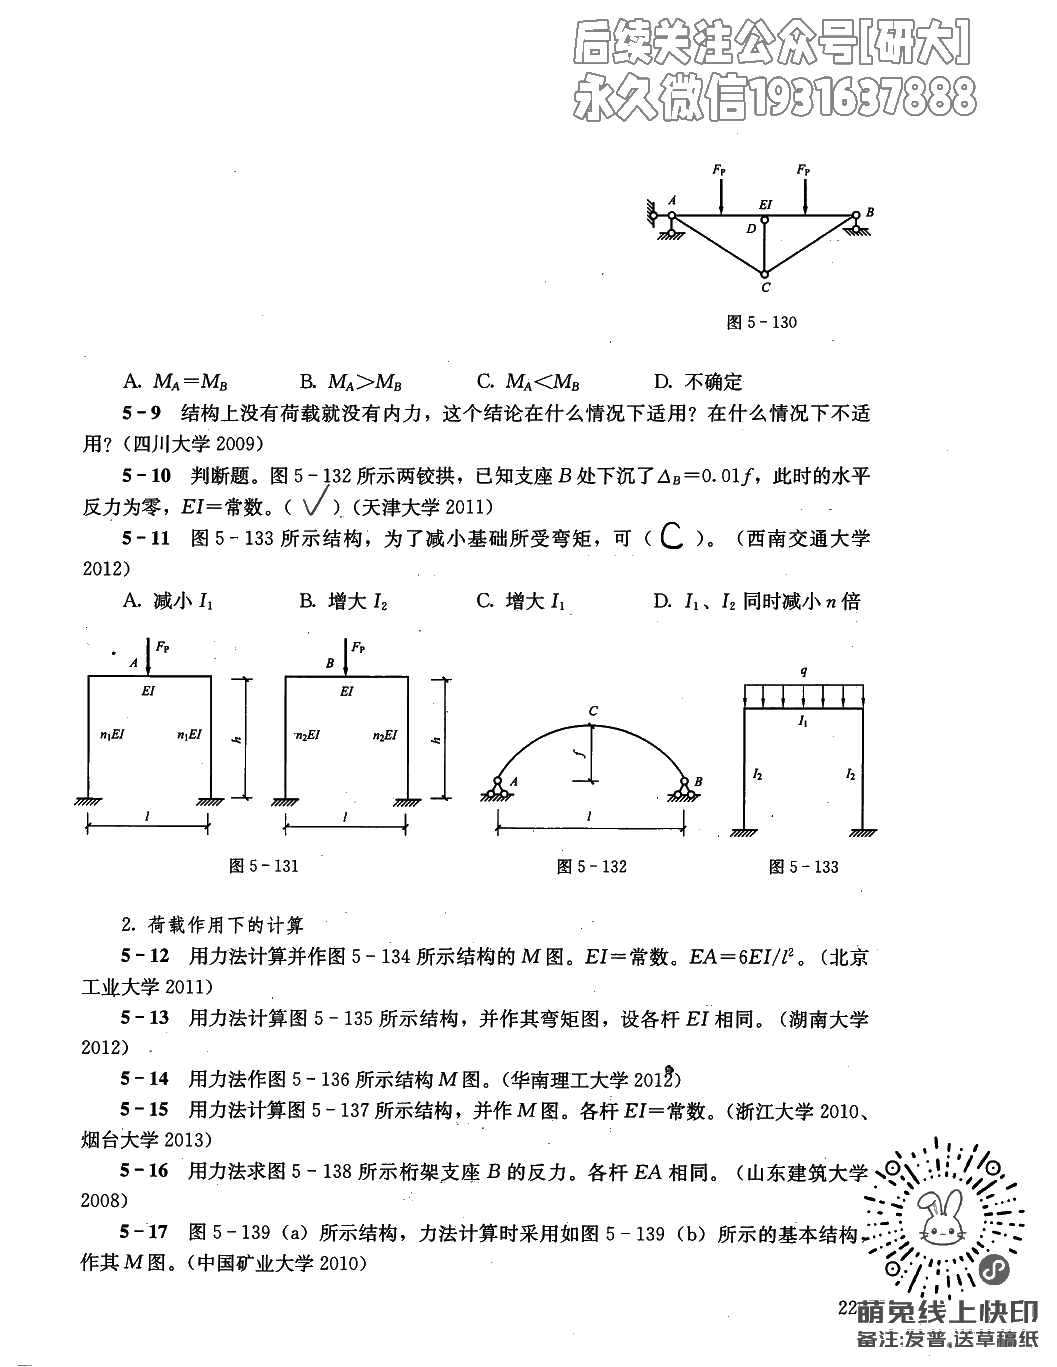
\includegraphics[width=0.96\textwidth,height=0.82\textheight,keepaspectratio]{images/c10_note_p04.png}
\par\small 讲解笔记（去水印版），第 4/21 页
\end{center}
\clearpage
\begin{center}
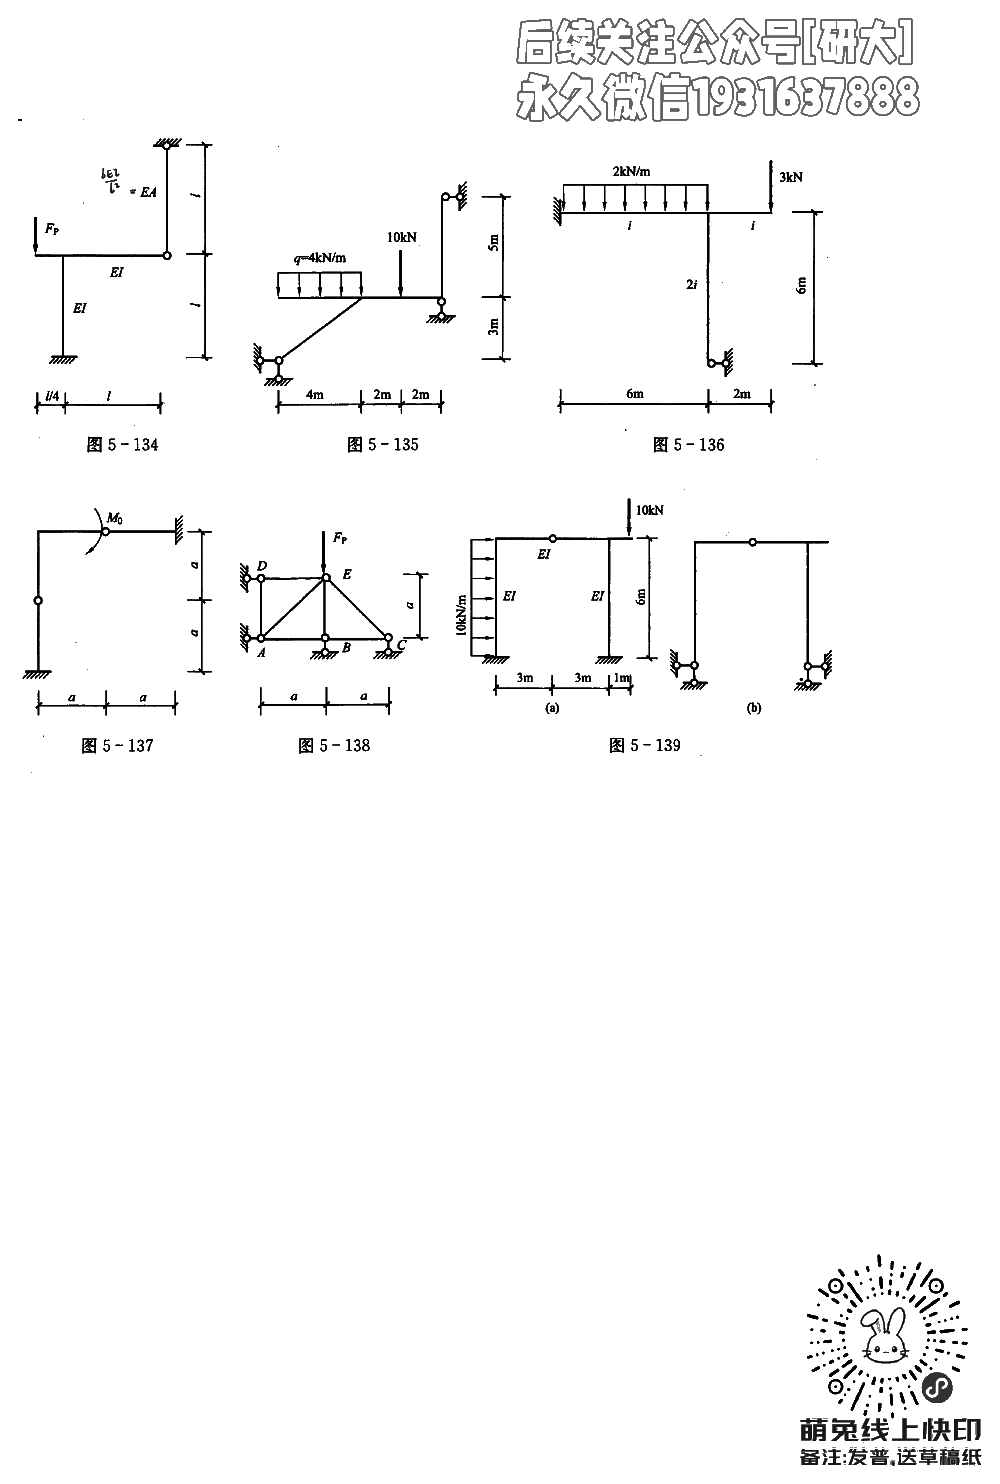
\includegraphics[width=0.96\textwidth,height=0.82\textheight,keepaspectratio]{images/c10_note_p05.png}
\par\small 讲解笔记（去水印版），第 5/21 页
\end{center}
\clearpage
\begin{center}
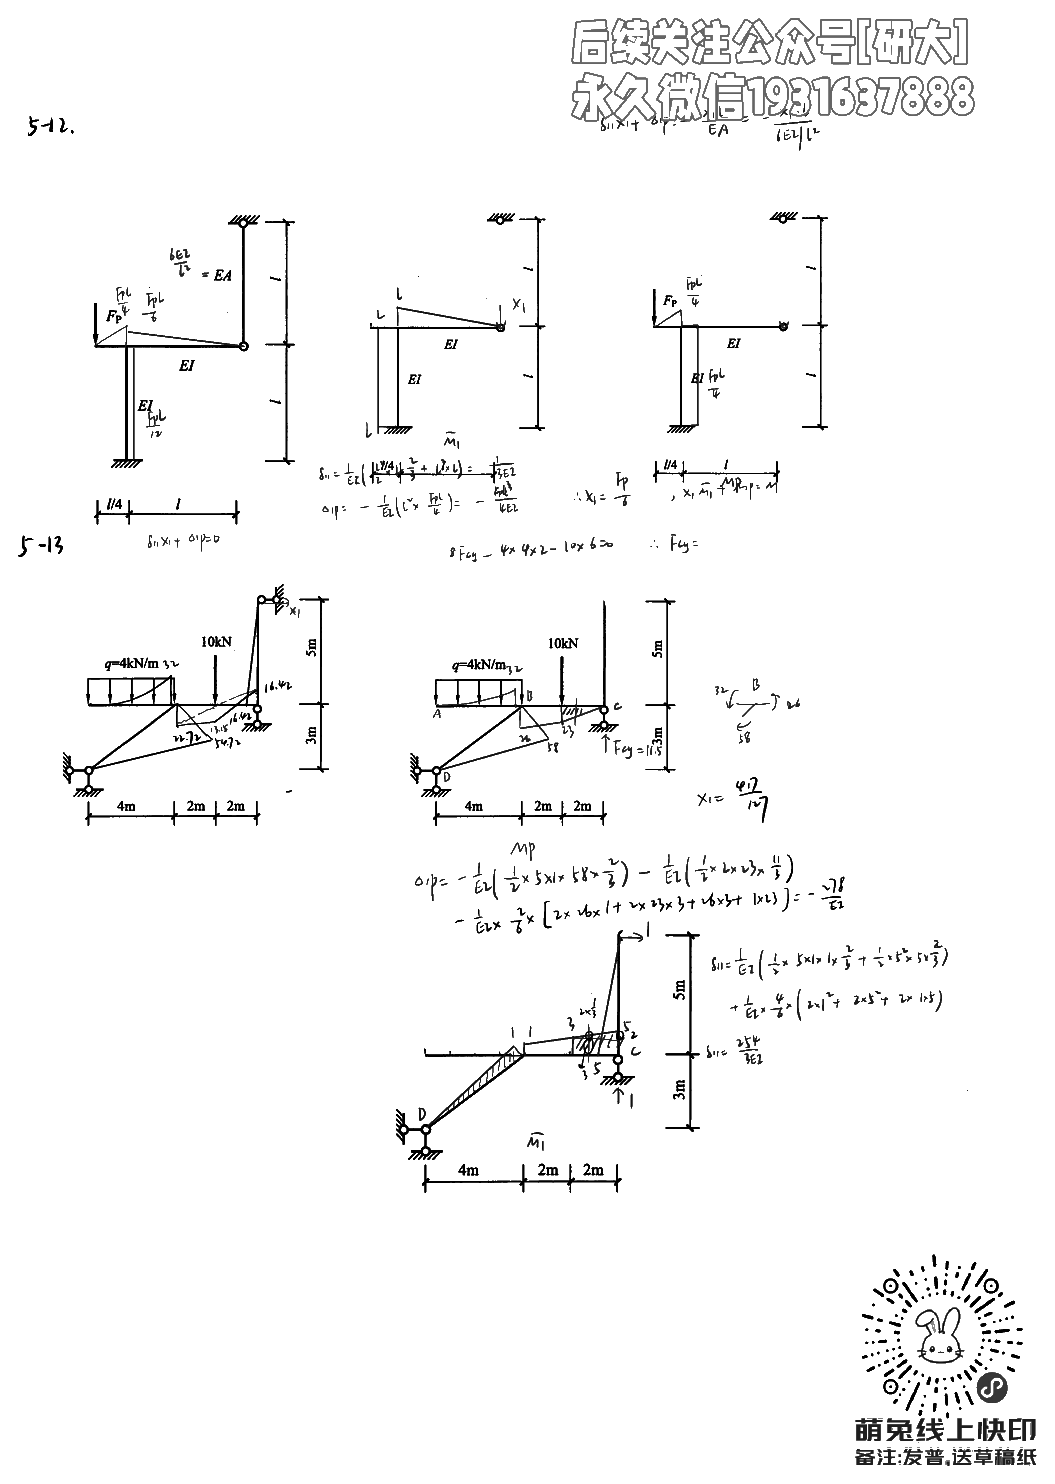
\includegraphics[width=0.96\textwidth,height=0.82\textheight,keepaspectratio]{images/c10_note_p06.png}
\par\small 讲解笔记（去水印版），第 6/21 页
\end{center}
\clearpage
\begin{center}
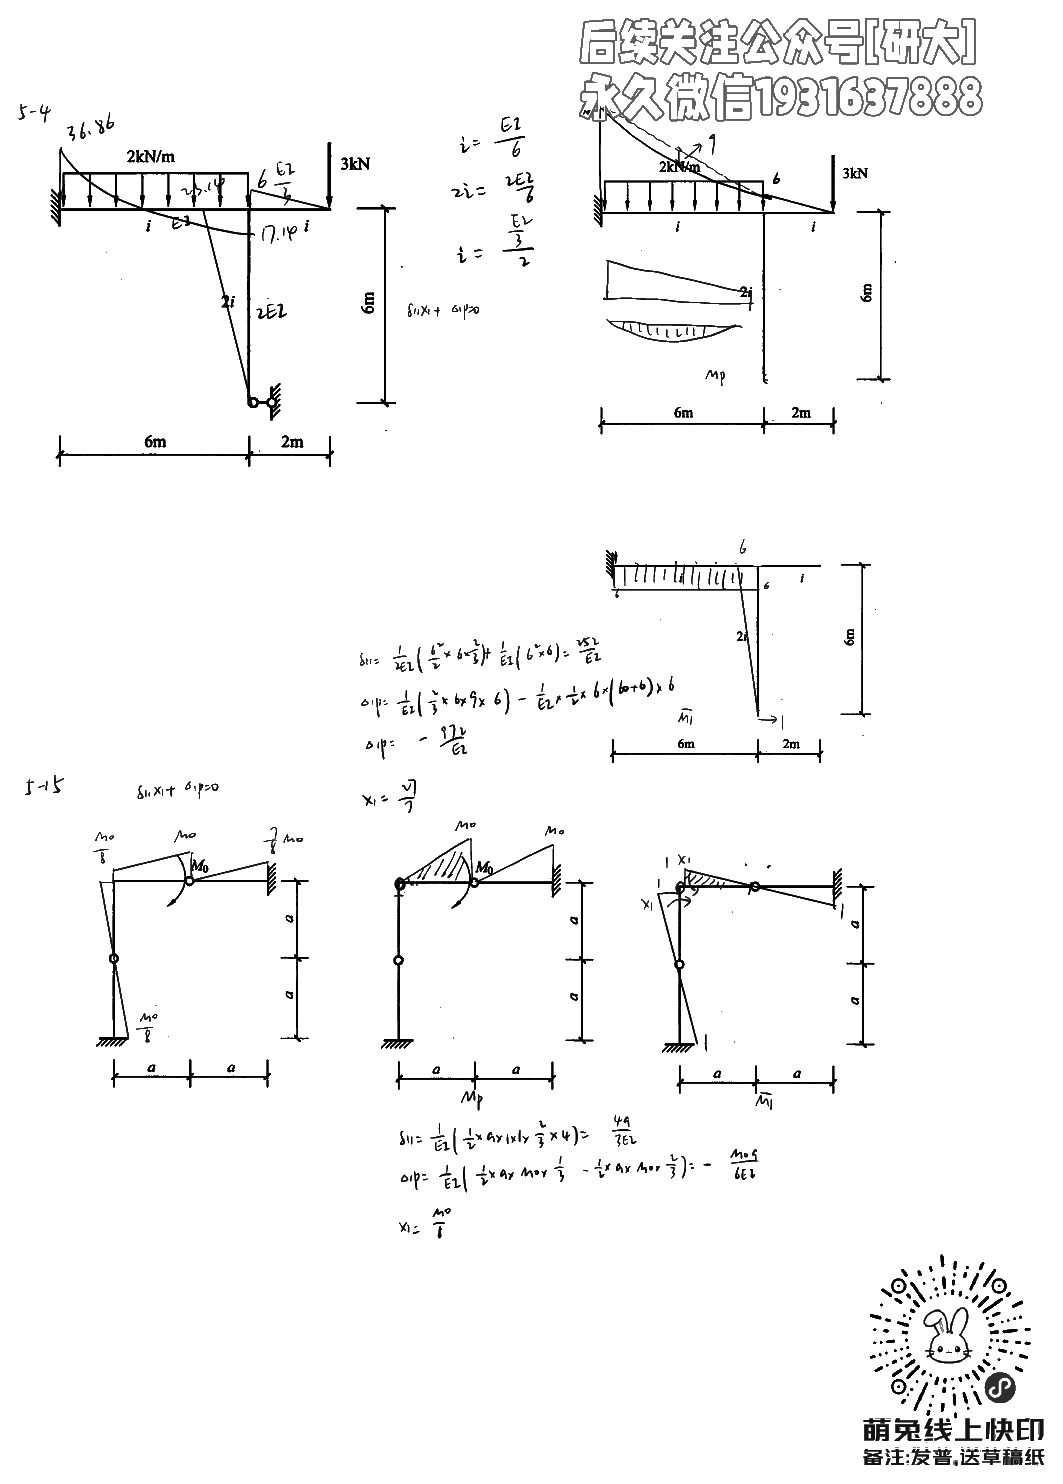
\includegraphics[width=0.96\textwidth,height=0.82\textheight,keepaspectratio]{images/c10_note_p07.png}
\par\small 讲解笔记（去水印版），第 7/21 页
\end{center}
\clearpage
\begin{center}
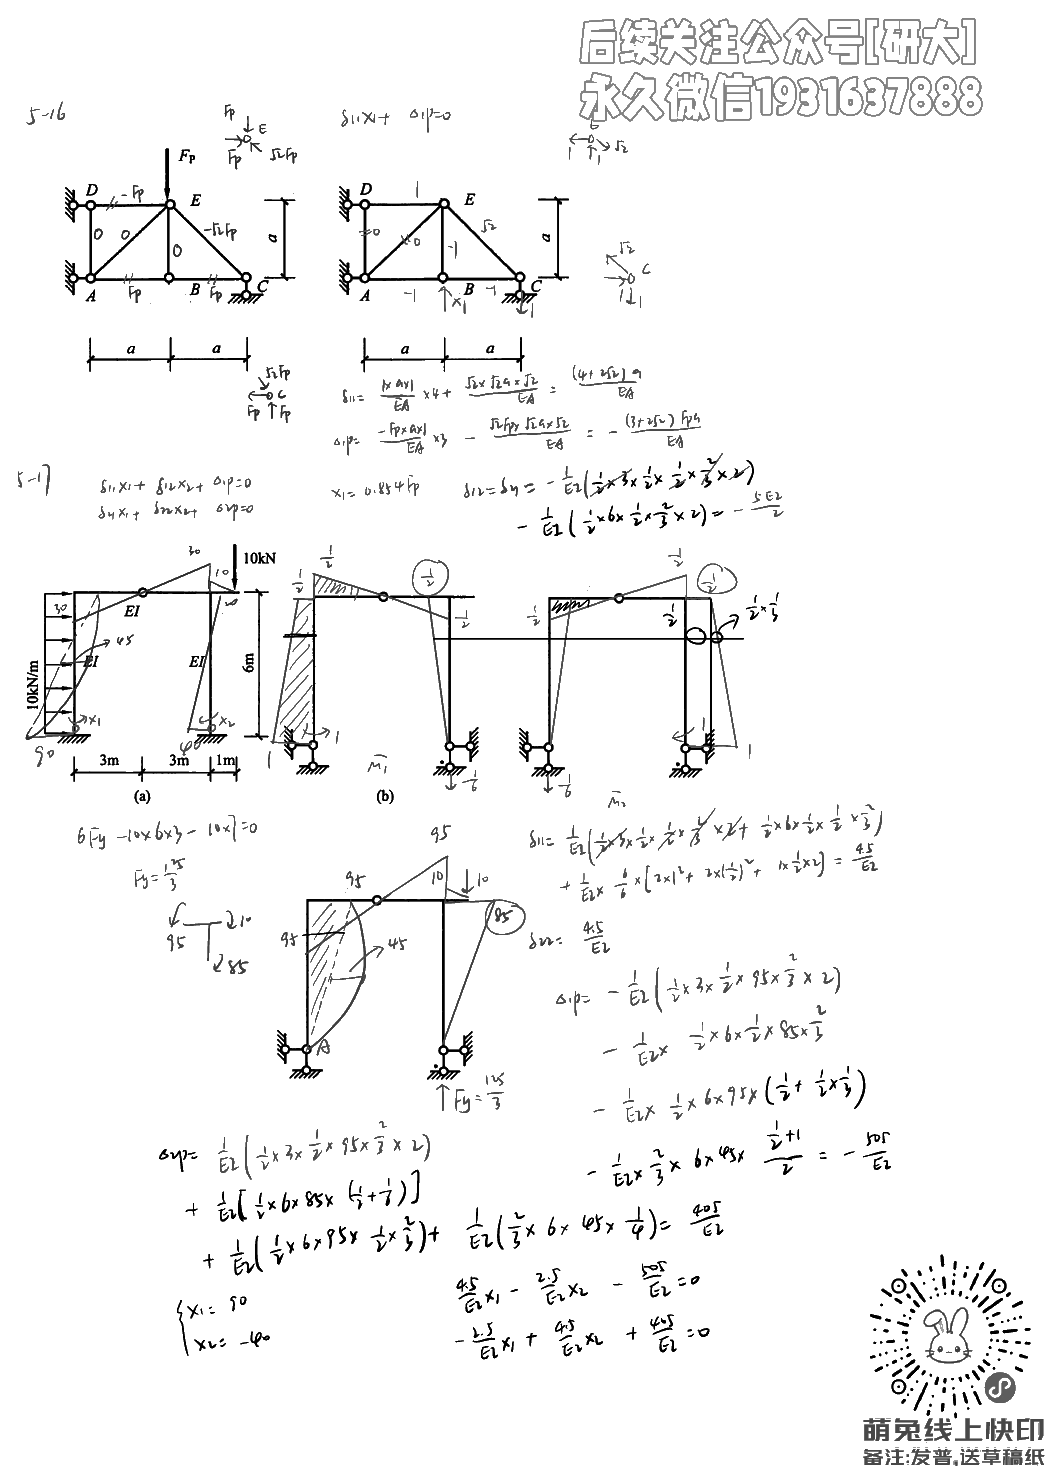
\includegraphics[width=0.96\textwidth,height=0.82\textheight,keepaspectratio]{images/c10_note_p08.png}
\par\small 讲解笔记（去水印版），第 8/21 页
\end{center}
\clearpage
\begin{center}
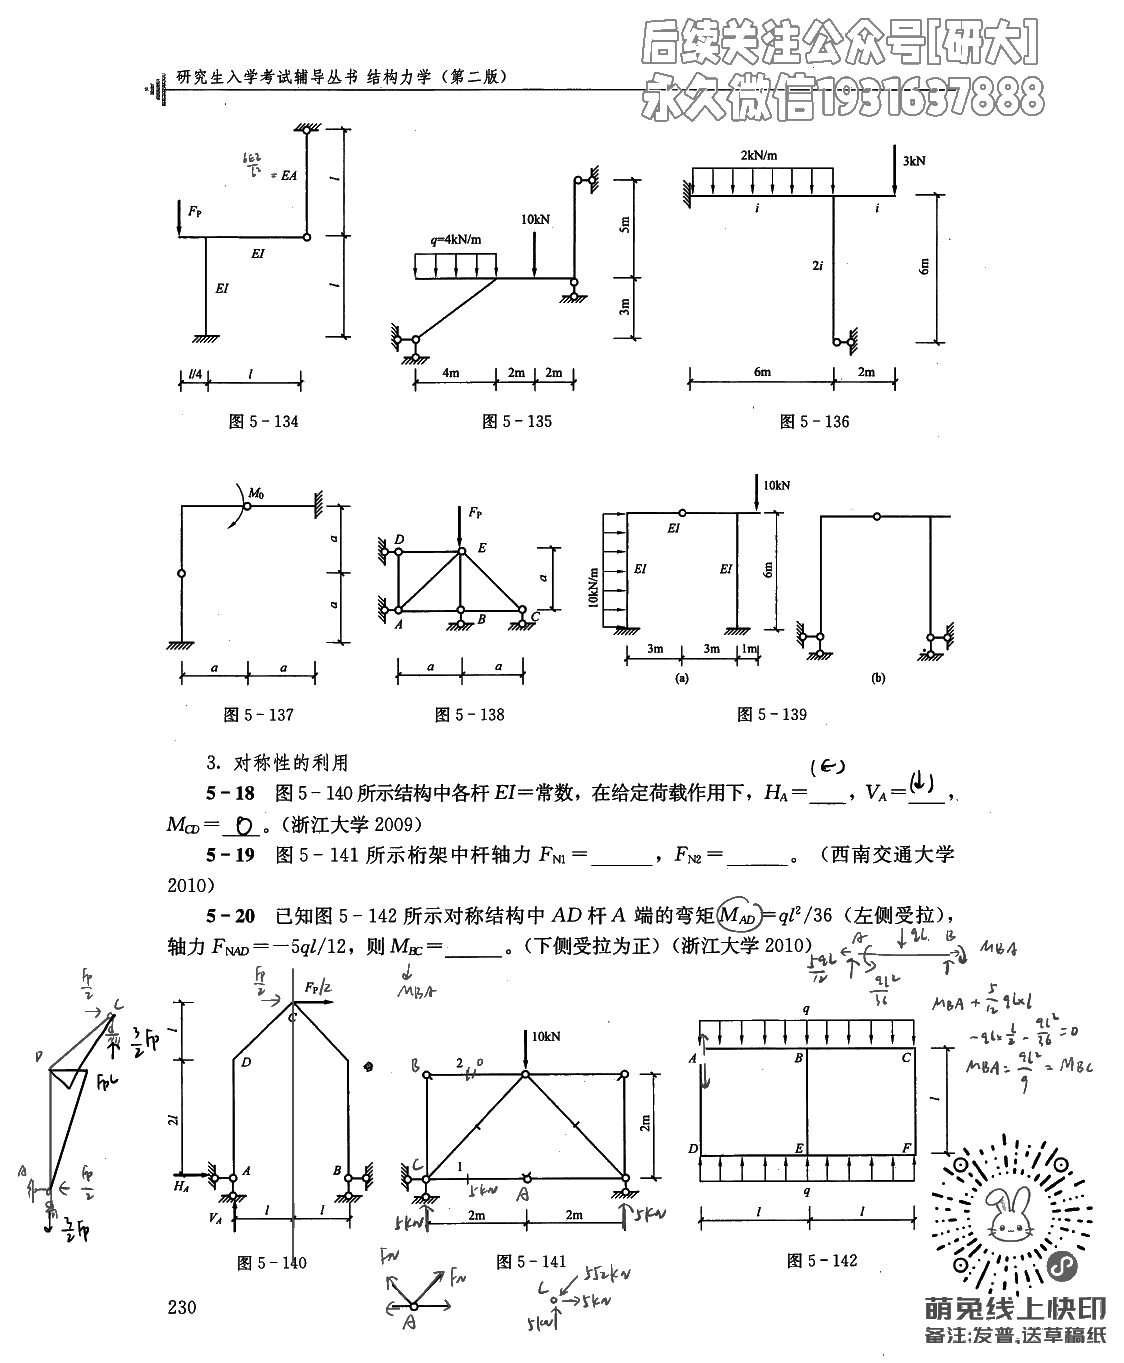
\includegraphics[width=0.96\textwidth,height=0.82\textheight,keepaspectratio]{images/c10_note_p09.png}
\par\small 讲解笔记（去水印版），第 9/21 页
\end{center}
\clearpage
\begin{center}
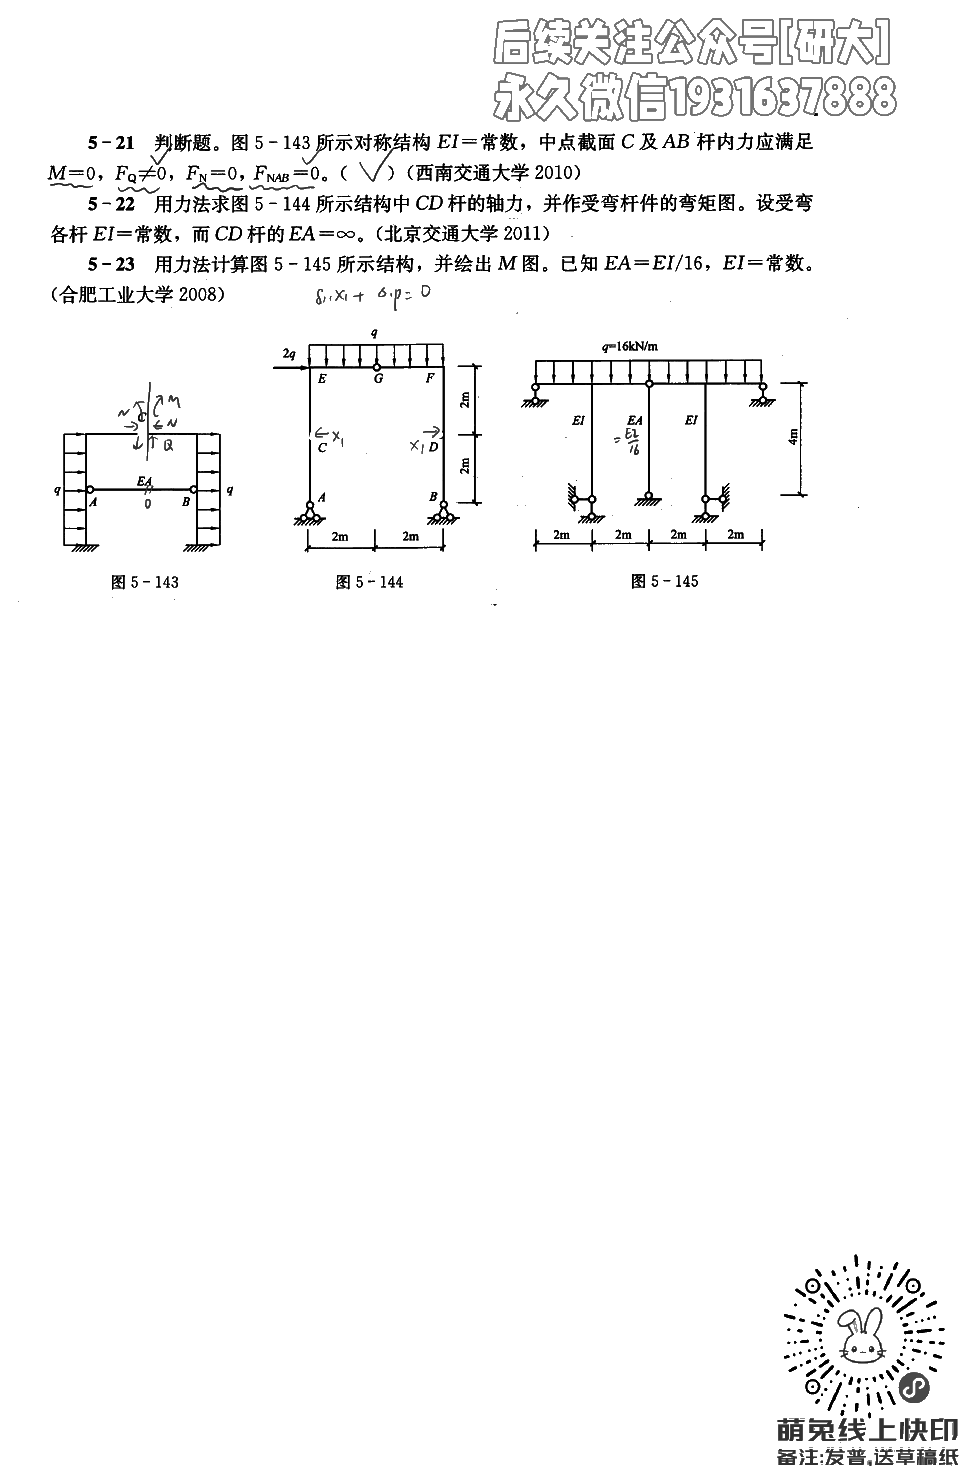
\includegraphics[width=0.96\textwidth,height=0.82\textheight,keepaspectratio]{images/c10_note_p10.png}
\par\small 讲解笔记（去水印版），第 10/21 页
\end{center}
\clearpage
\begin{center}
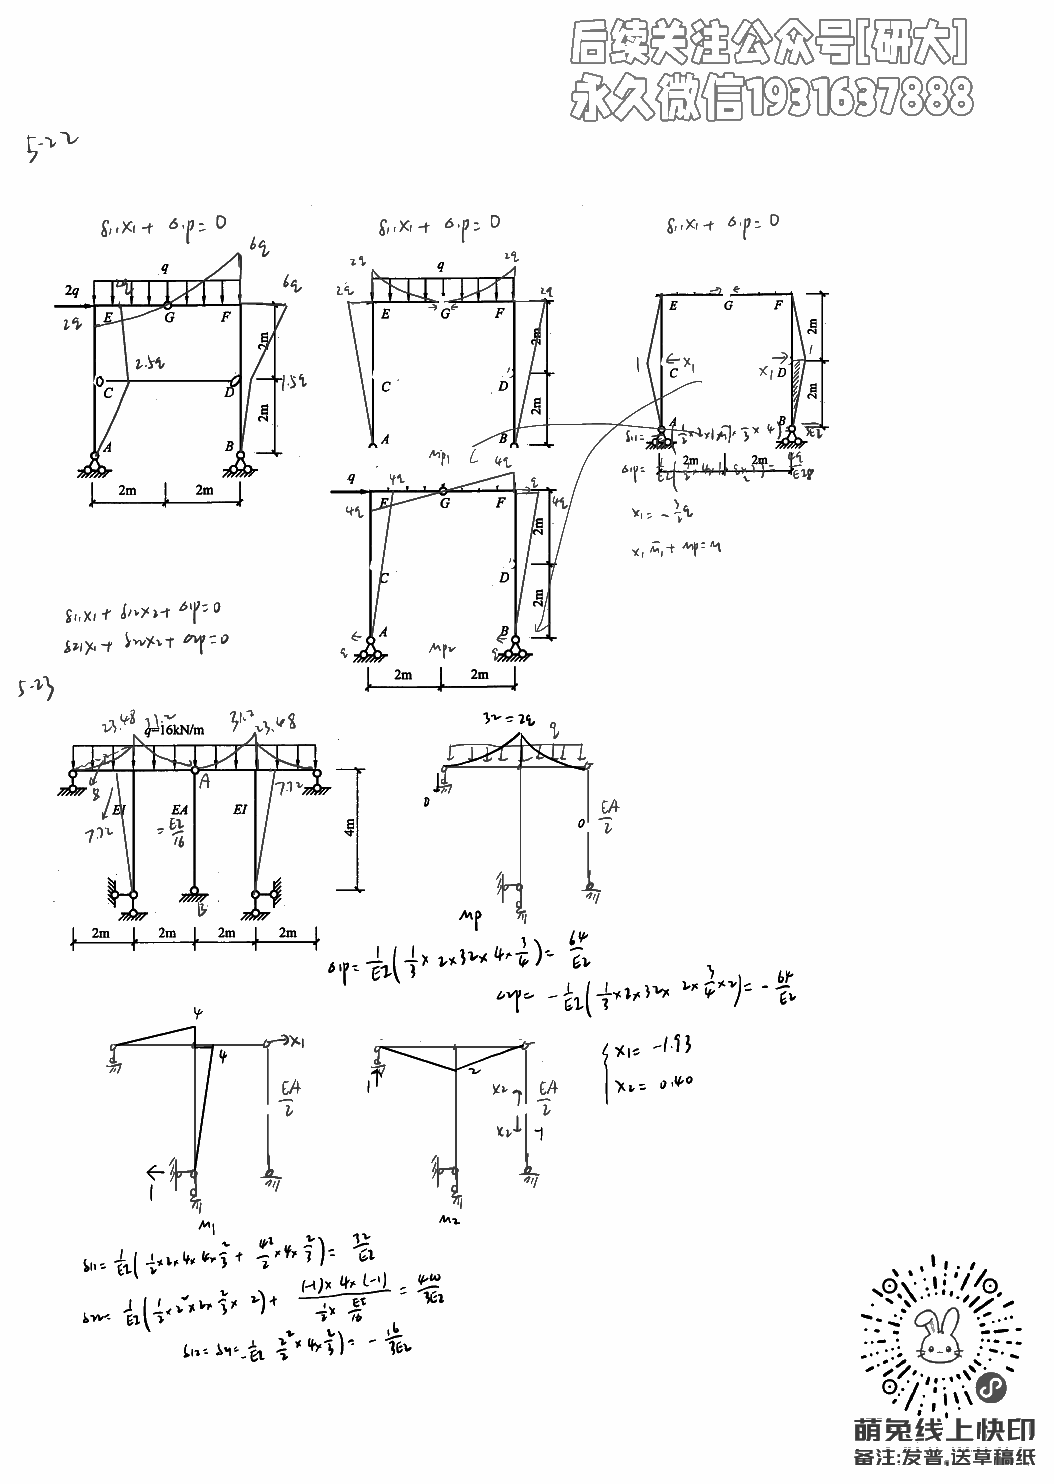
\includegraphics[width=0.96\textwidth,height=0.82\textheight,keepaspectratio]{images/c10_note_p11.png}
\par\small 讲解笔记（去水印版），第 11/21 页
\end{center}
\clearpage
\begin{center}
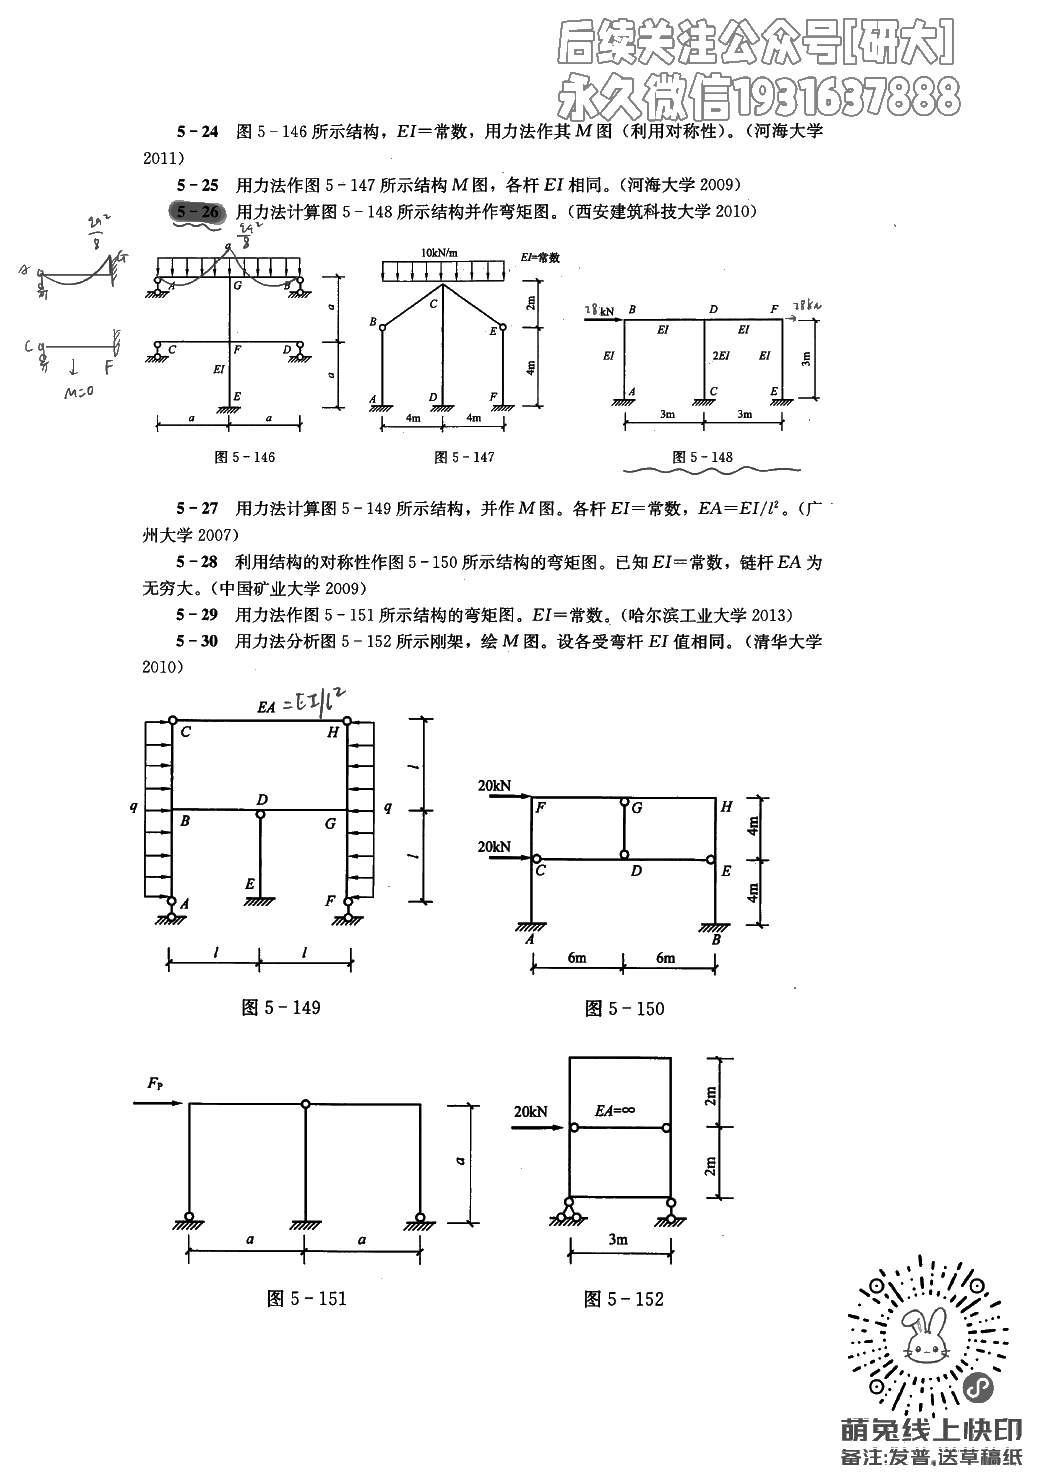
\includegraphics[width=0.96\textwidth,height=0.82\textheight,keepaspectratio]{images/c10_note_p12.png}
\par\small 讲解笔记（去水印版），第 12/21 页
\end{center}
\clearpage
\begin{center}
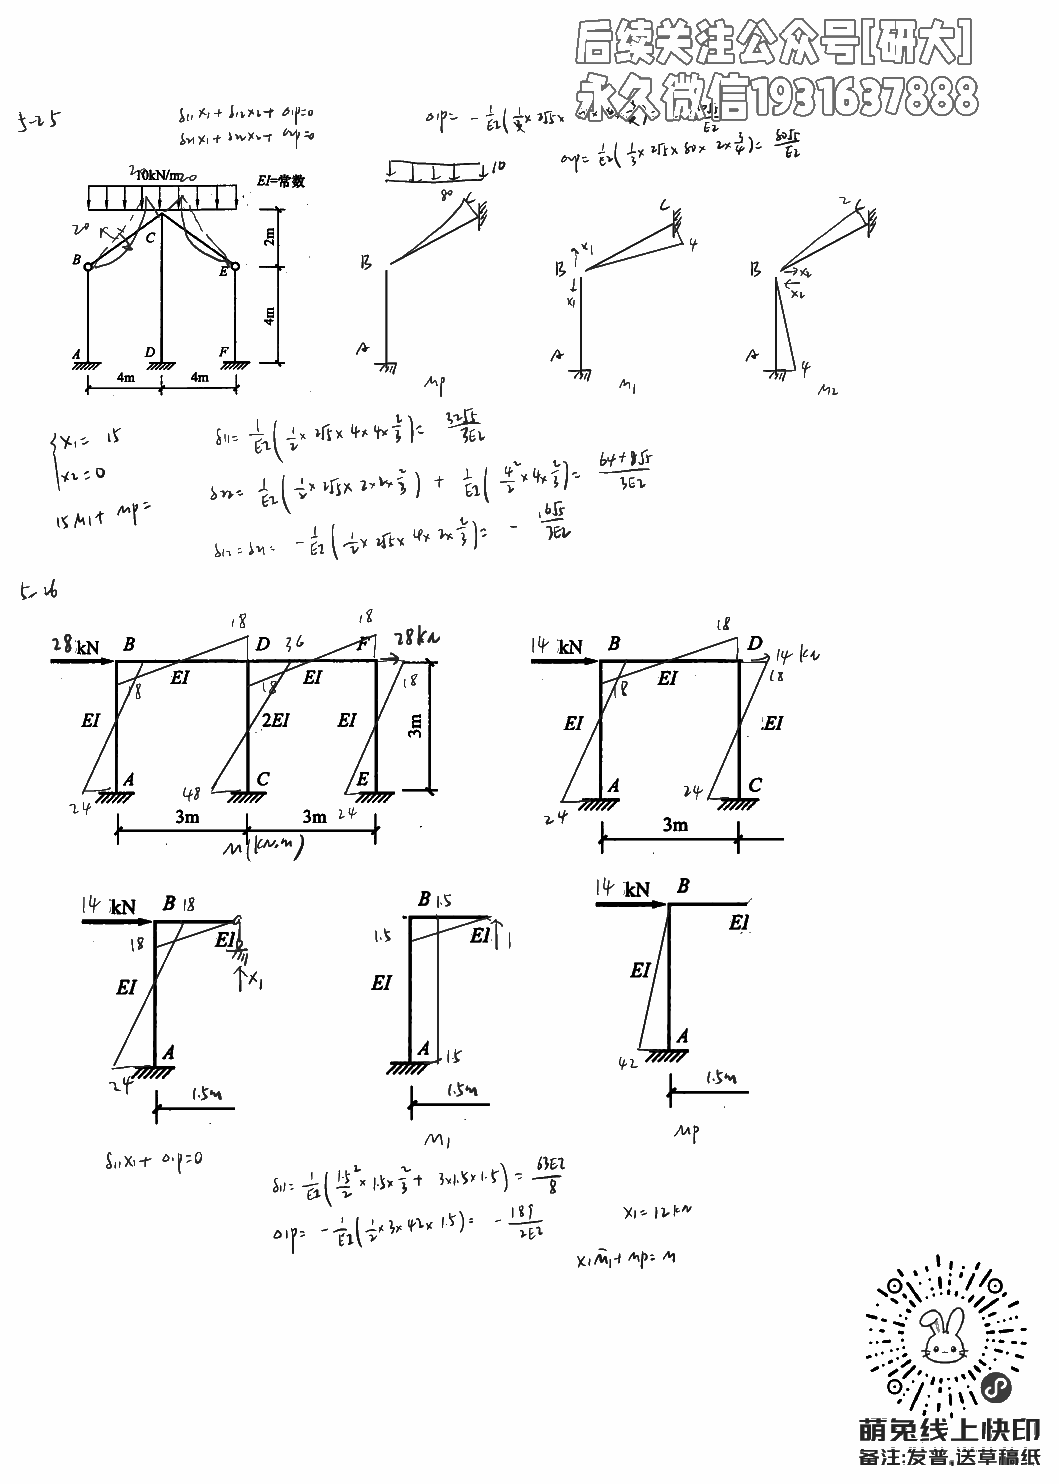
\includegraphics[width=0.96\textwidth,height=0.82\textheight,keepaspectratio]{images/c10_note_p13.png}
\par\small 讲解笔记（去水印版），第 13/21 页
\end{center}
\clearpage
\begin{center}
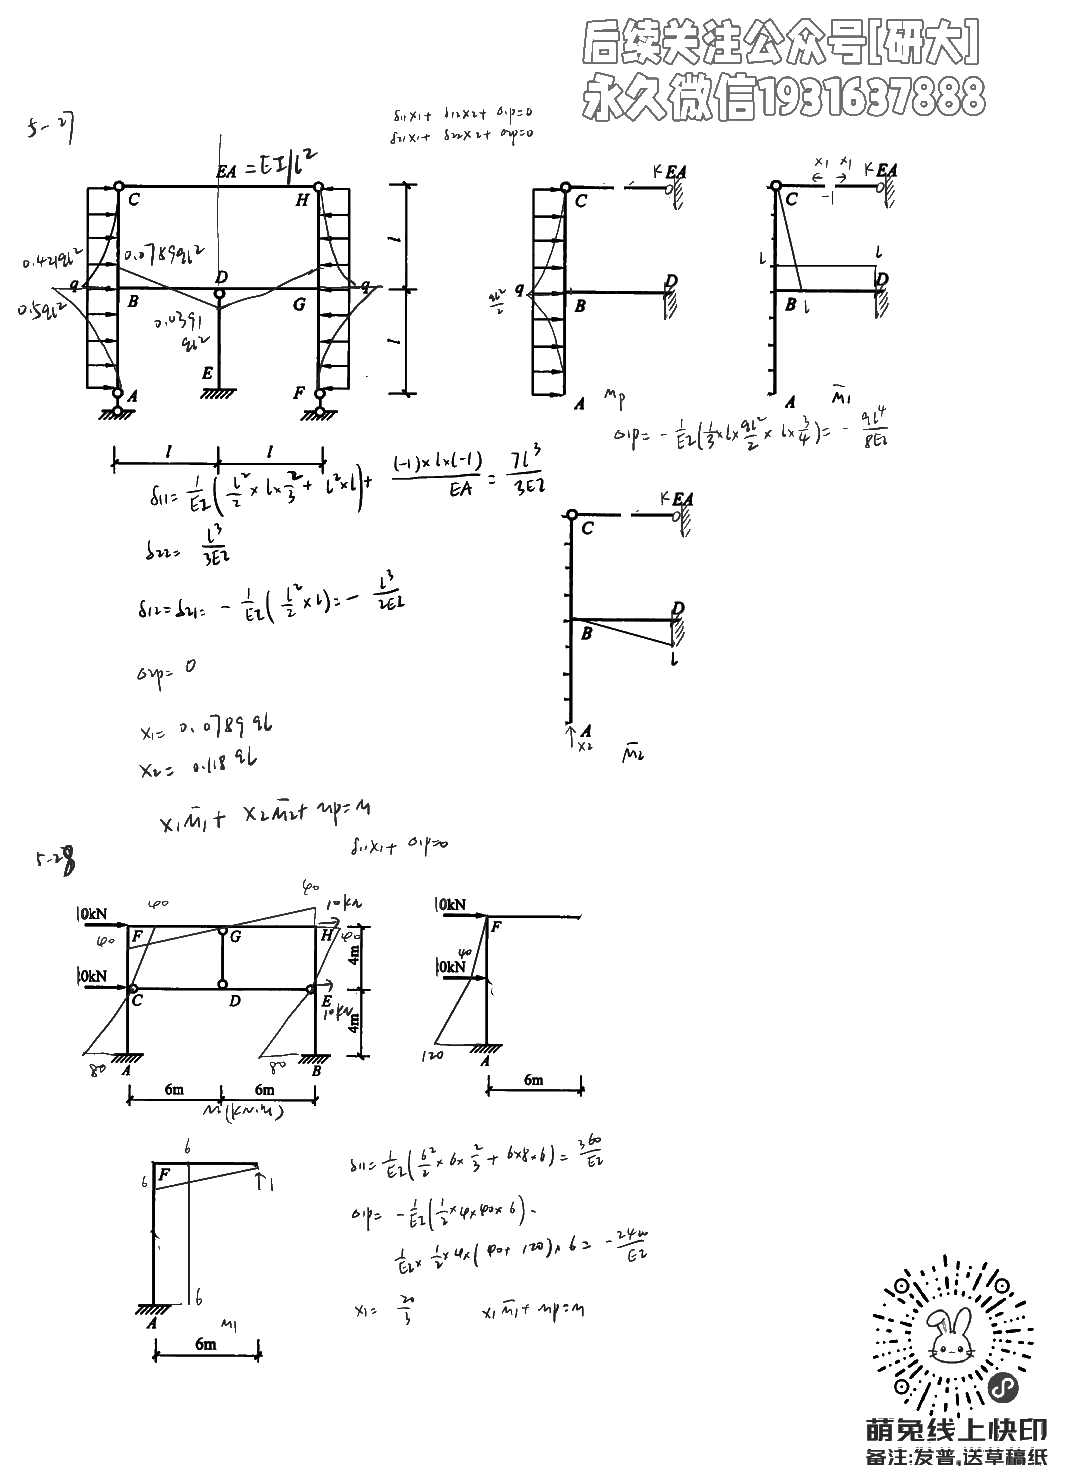
\includegraphics[width=0.96\textwidth,height=0.82\textheight,keepaspectratio]{images/c10_note_p14.png}
\par\small 讲解笔记（去水印版），第 14/21 页
\end{center}
\clearpage
\begin{center}
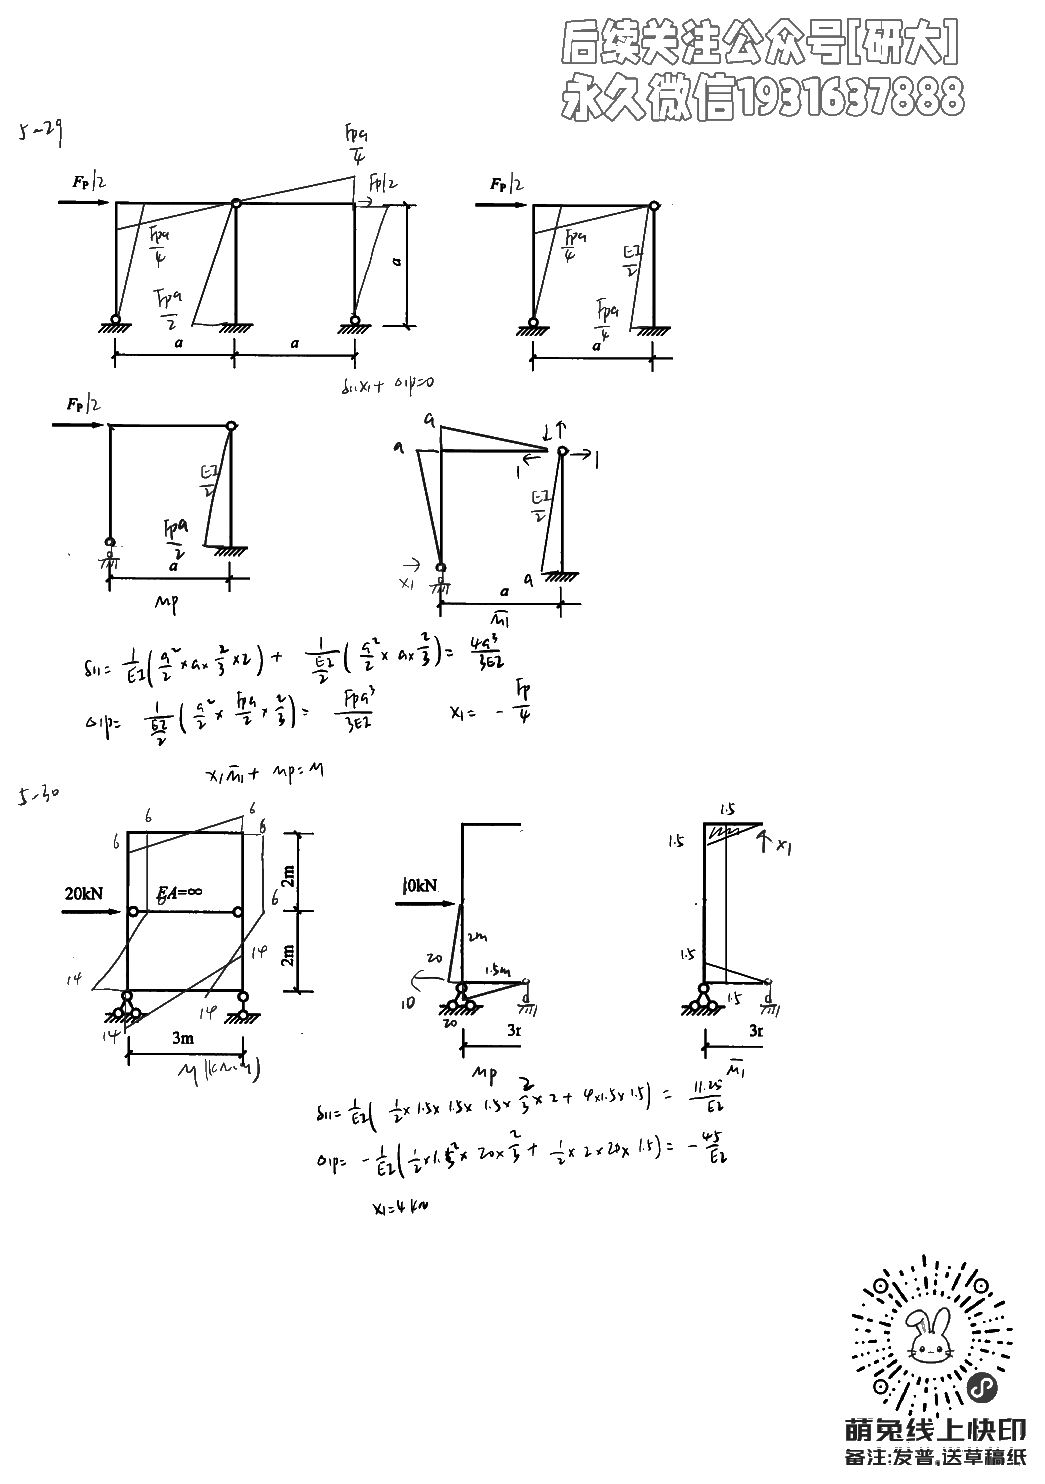
\includegraphics[width=0.96\textwidth,height=0.82\textheight,keepaspectratio]{images/c10_note_p15.png}
\par\small 讲解笔记（去水印版），第 15/21 页
\end{center}
\clearpage
\begin{center}
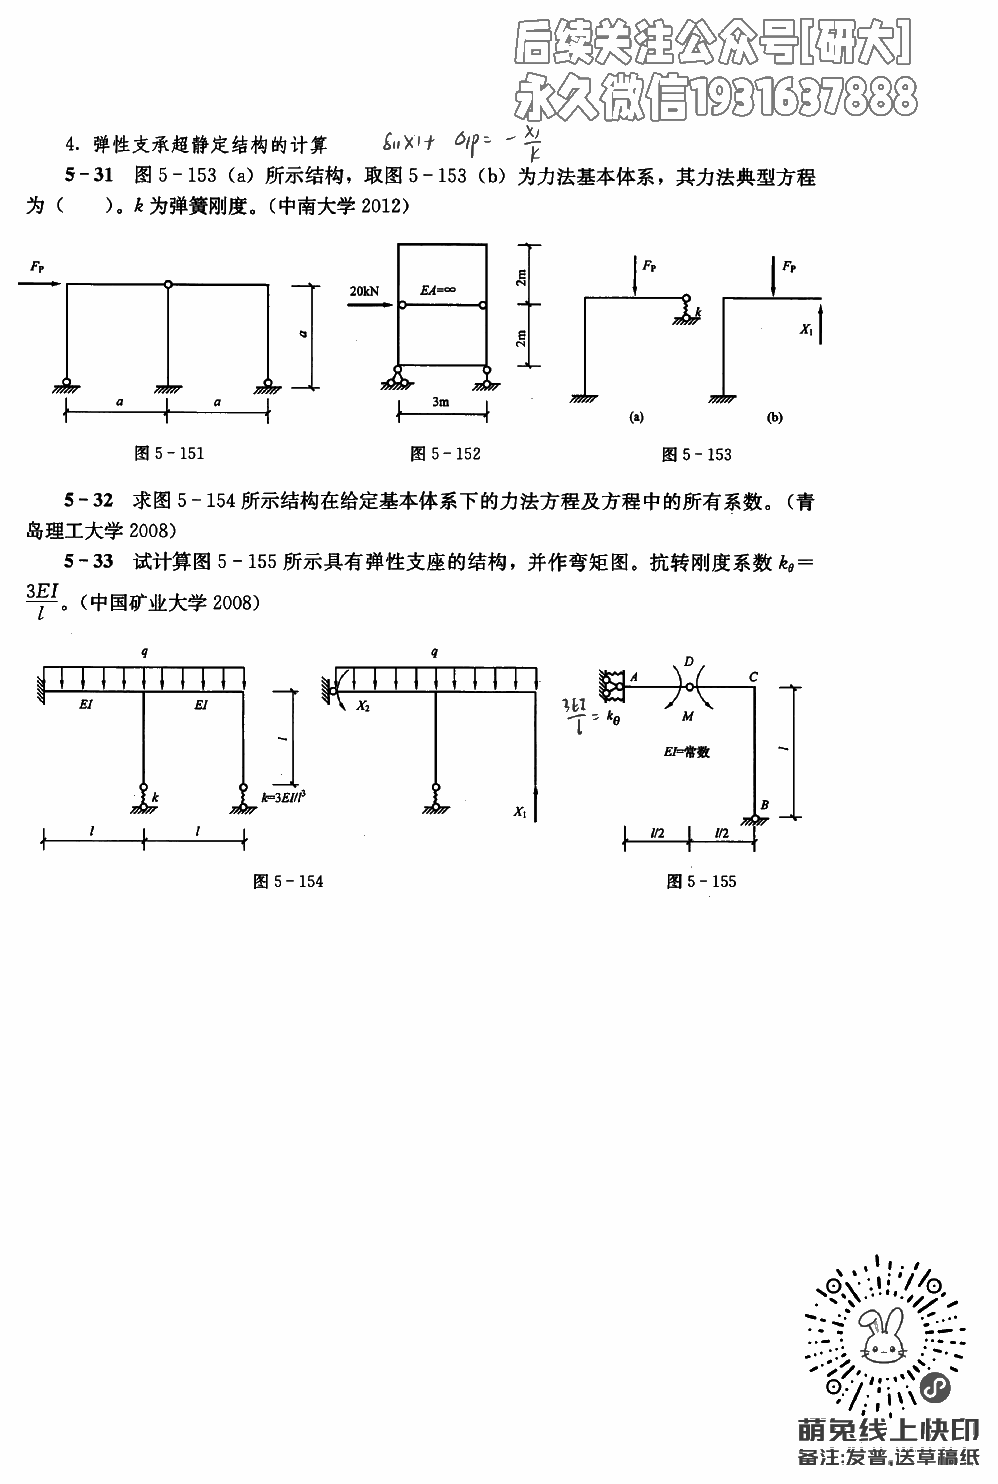
\includegraphics[width=0.96\textwidth,height=0.82\textheight,keepaspectratio]{images/c10_note_p16.png}
\par\small 讲解笔记（去水印版），第 16/21 页
\end{center}
\clearpage
\begin{center}
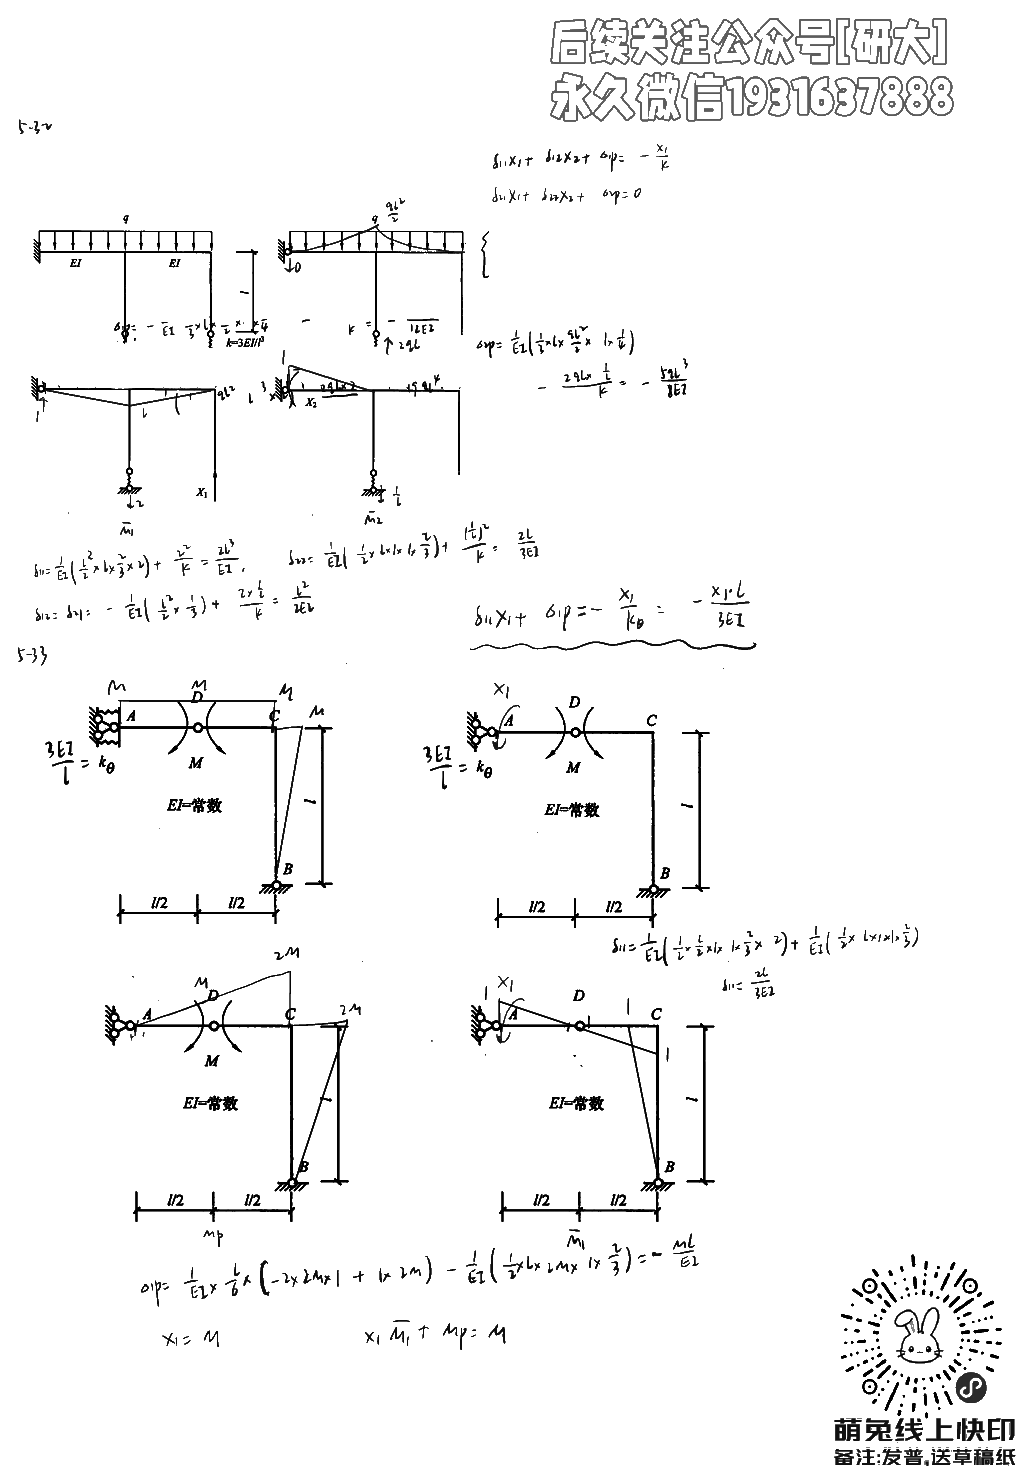
\includegraphics[width=0.96\textwidth,height=0.82\textheight,keepaspectratio]{images/c10_note_p17.png}
\par\small 讲解笔记（去水印版），第 17/21 页
\end{center}
\clearpage
\begin{center}
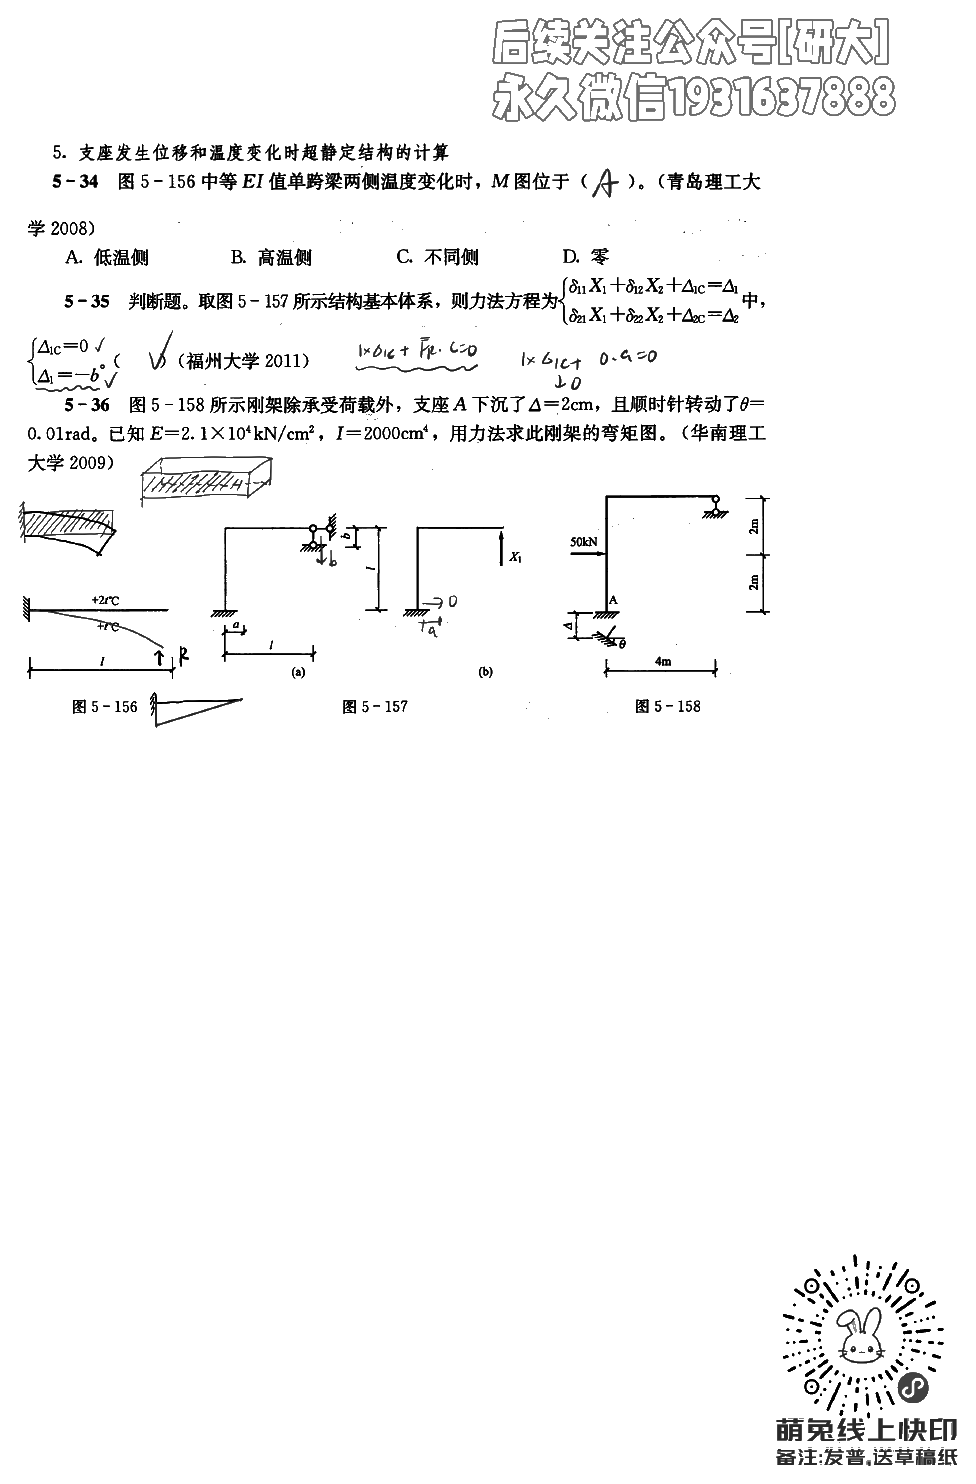
\includegraphics[width=0.96\textwidth,height=0.82\textheight,keepaspectratio]{images/c10_note_p18.png}
\par\small 讲解笔记（去水印版），第 18/21 页
\end{center}
\clearpage
\begin{center}
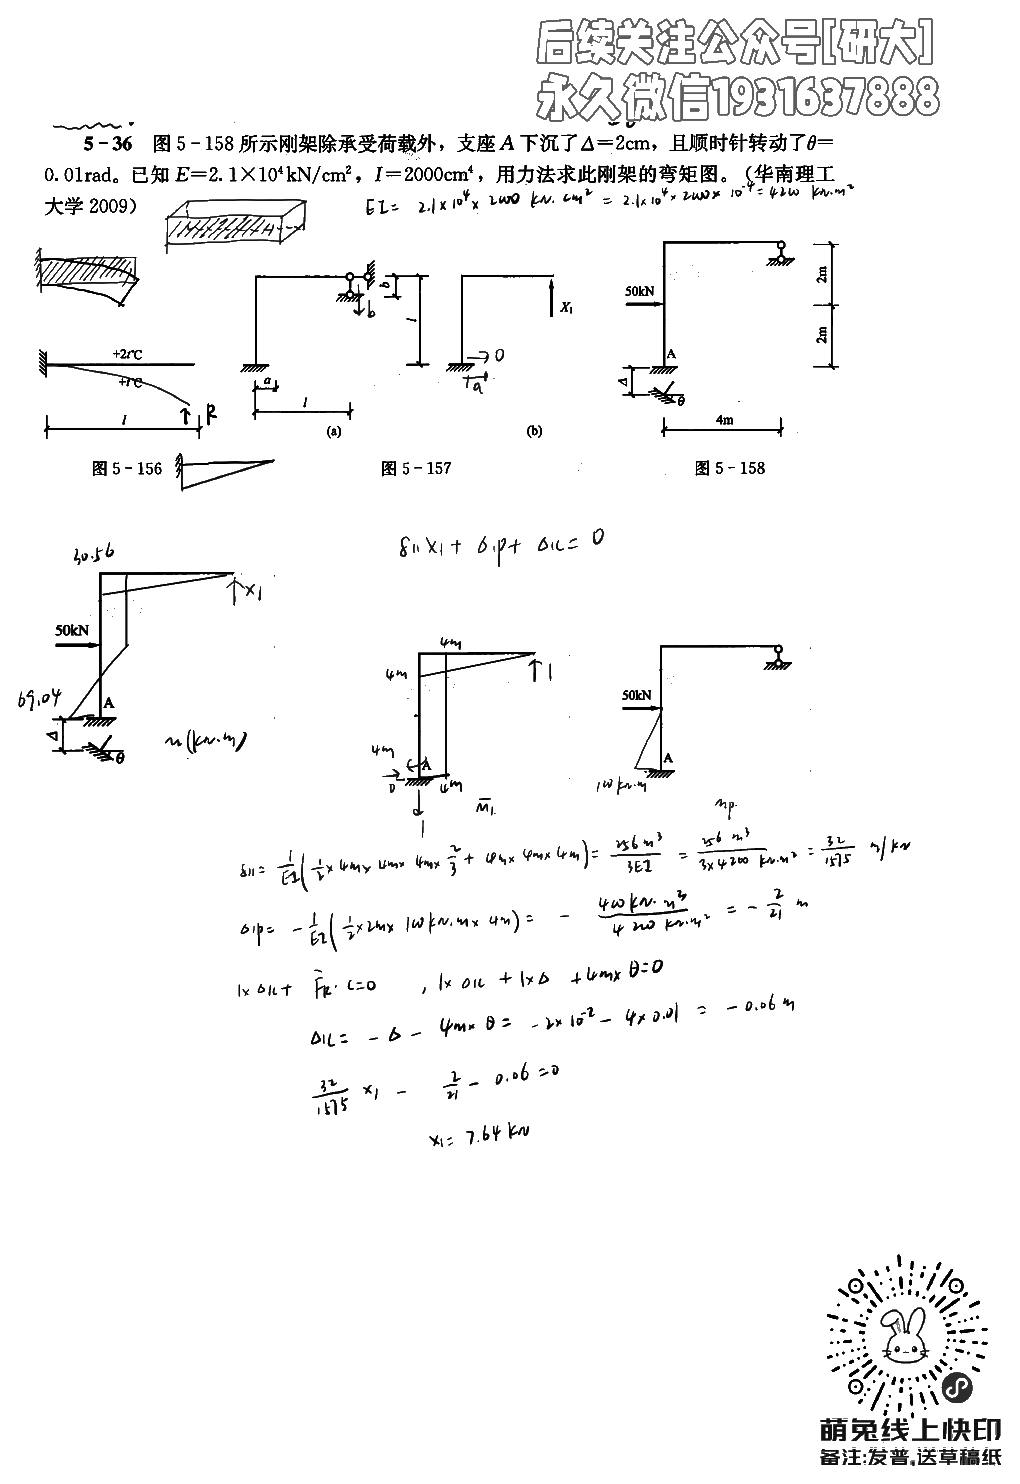
\includegraphics[width=0.96\textwidth,height=0.82\textheight,keepaspectratio]{images/c10_note_p19.png}
\par\small 讲解笔记（去水印版），第 19/21 页
\end{center}
\clearpage
\begin{center}
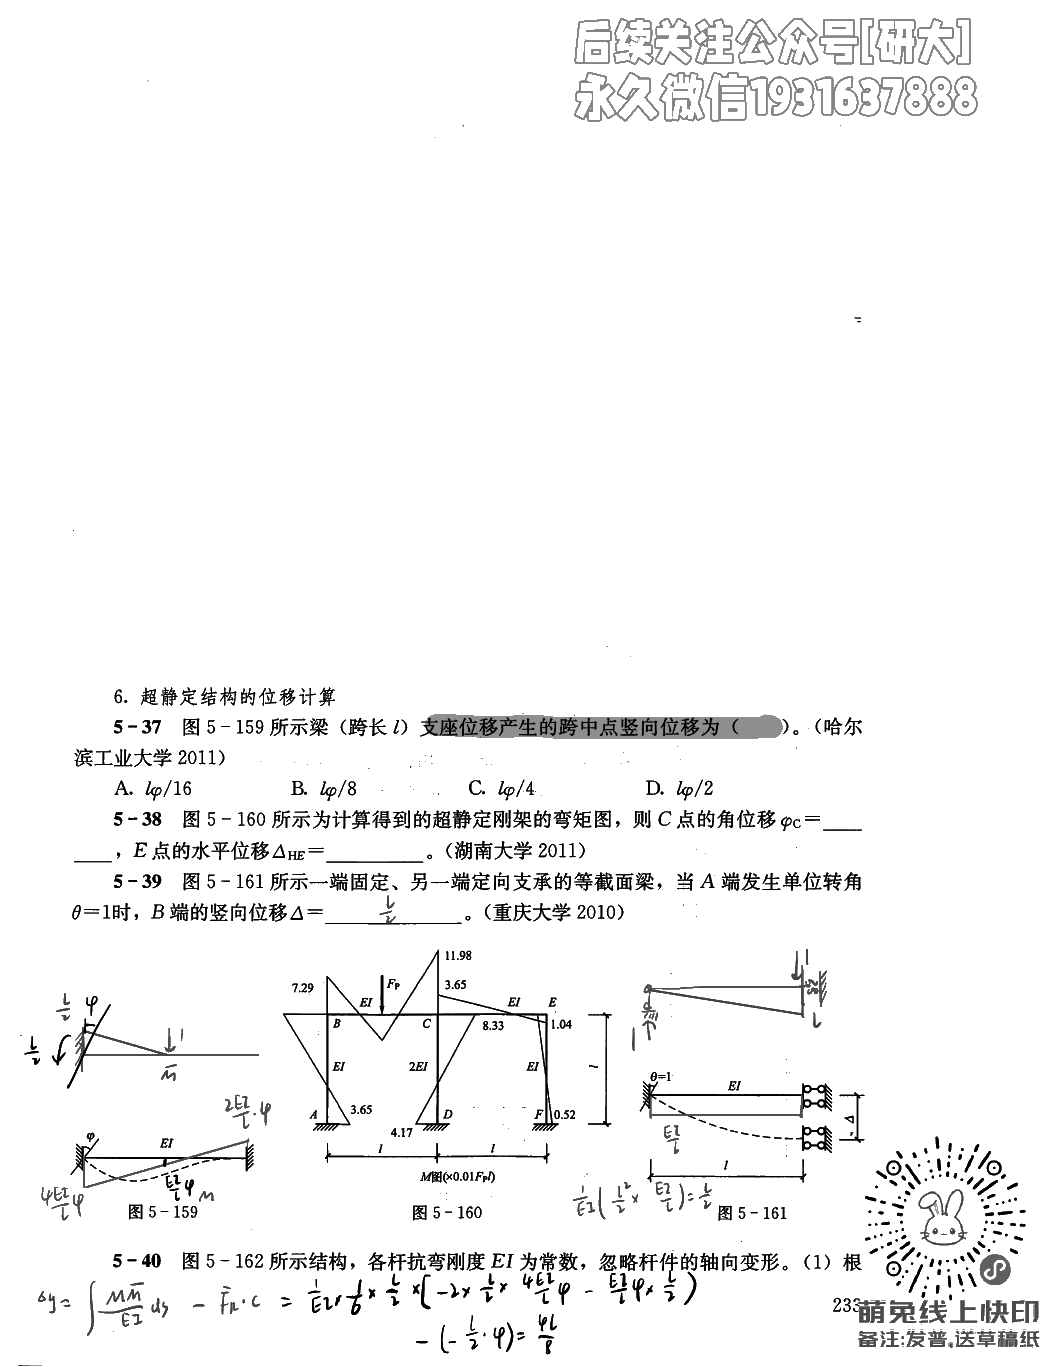
\includegraphics[width=0.96\textwidth,height=0.82\textheight,keepaspectratio]{images/c10_note_p20.png}
\par\small 讲解笔记（去水印版），第 20/21 页
\end{center}
\clearpage
\begin{center}
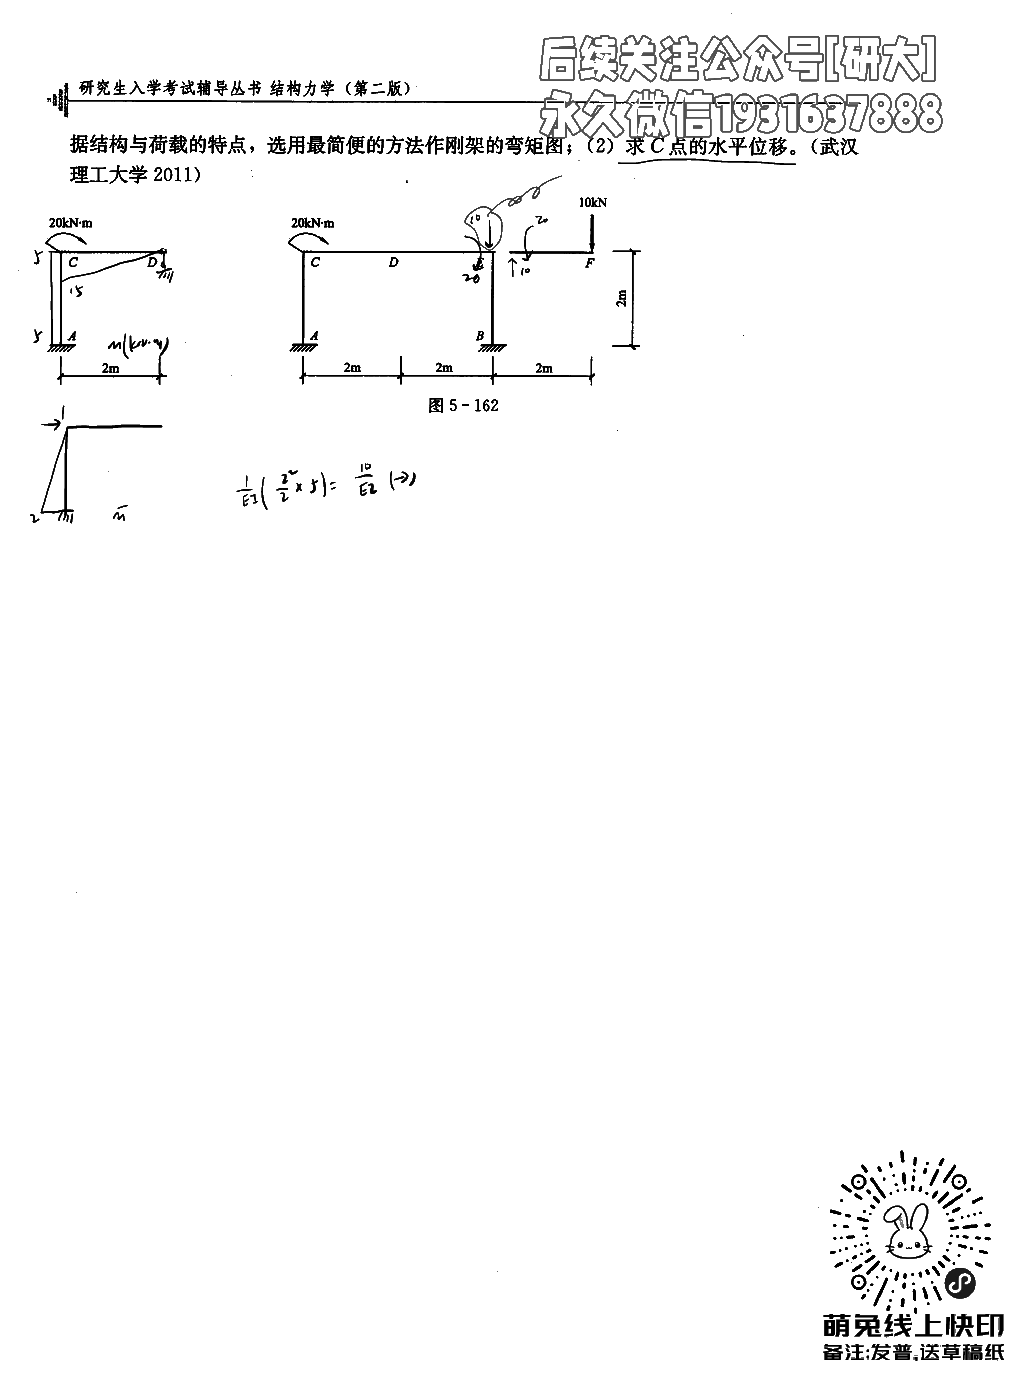
\includegraphics[width=0.96\textwidth,height=0.82\textheight,keepaspectratio]{images/c10_note_p21.png}
\par\small 讲解笔记（去水印版），第 21/21 页
\end{center}
\clearpage
\chapter{第11讲：力法（二）}
\begin{tcolorbox}[title=解析要点]
力法（二）通常题型更复杂，应重点检查基本未知力选择、单位力图、柔度系数对称性以及自由项符号。最终内力图必须满足原结构约束条件。
\end{tcolorbox}
\begin{tcolorbox}[title=答案与校核]
答案页给出力法（二）的方程与结果；柔度系数对称性和变形协调条件是主要检查点。
\end{tcolorbox}
\section{作业与答案（去水印版）}
\begin{center}
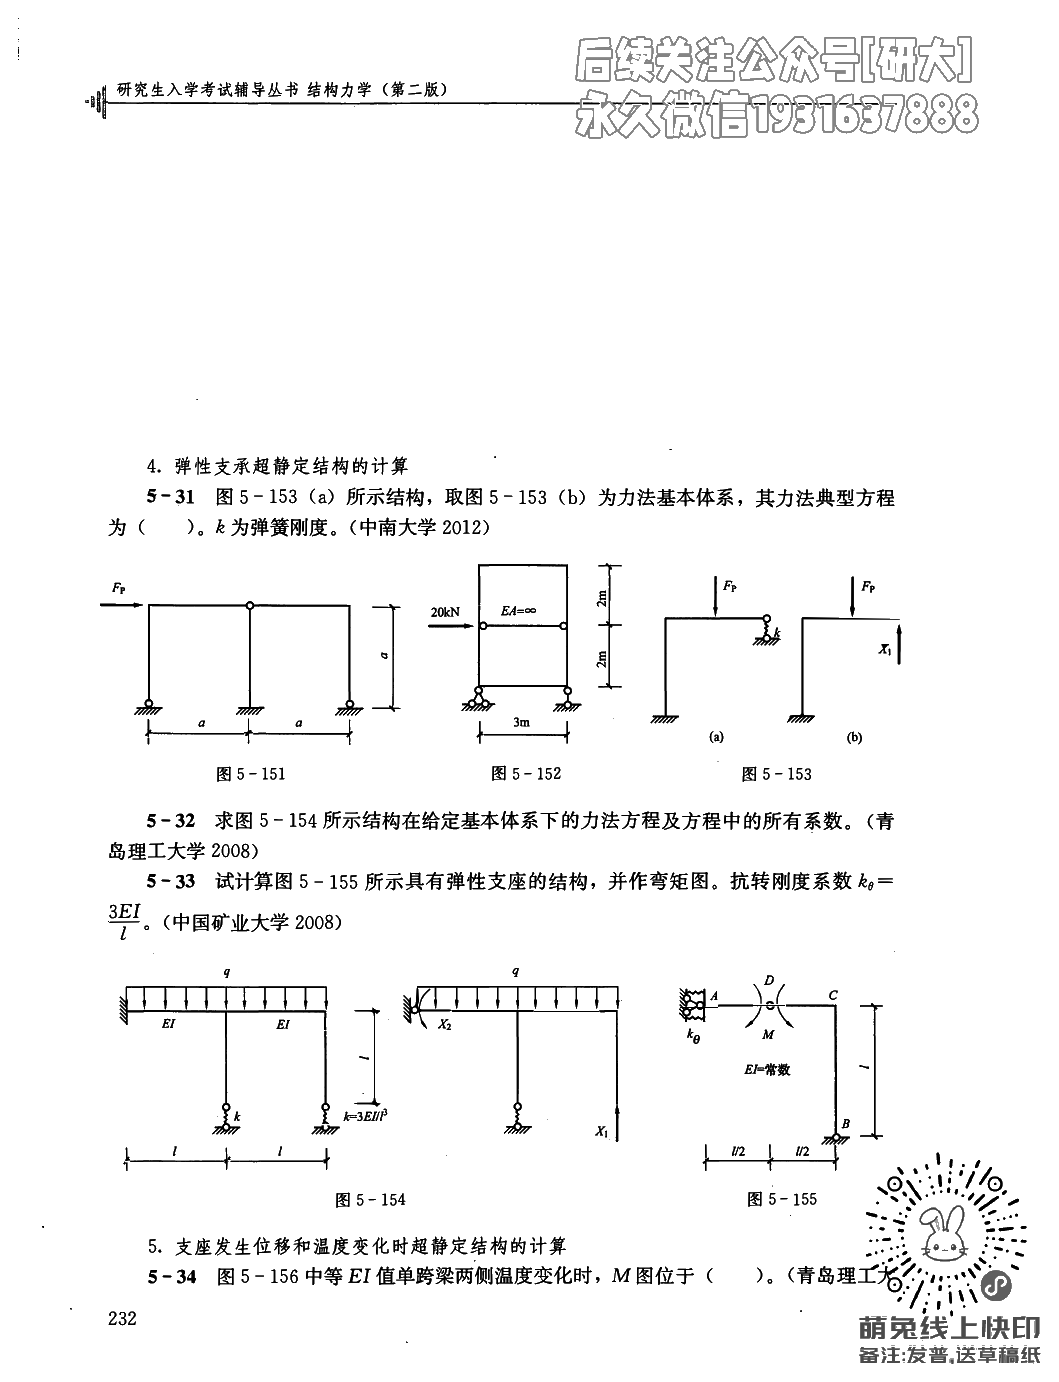
\includegraphics[width=0.96\textwidth,height=0.82\textheight,keepaspectratio]{images/c11_answer_1_p01.png}
\par\small 作业与答案（去水印版），第 1/8 页
\end{center}
\clearpage
\begin{center}
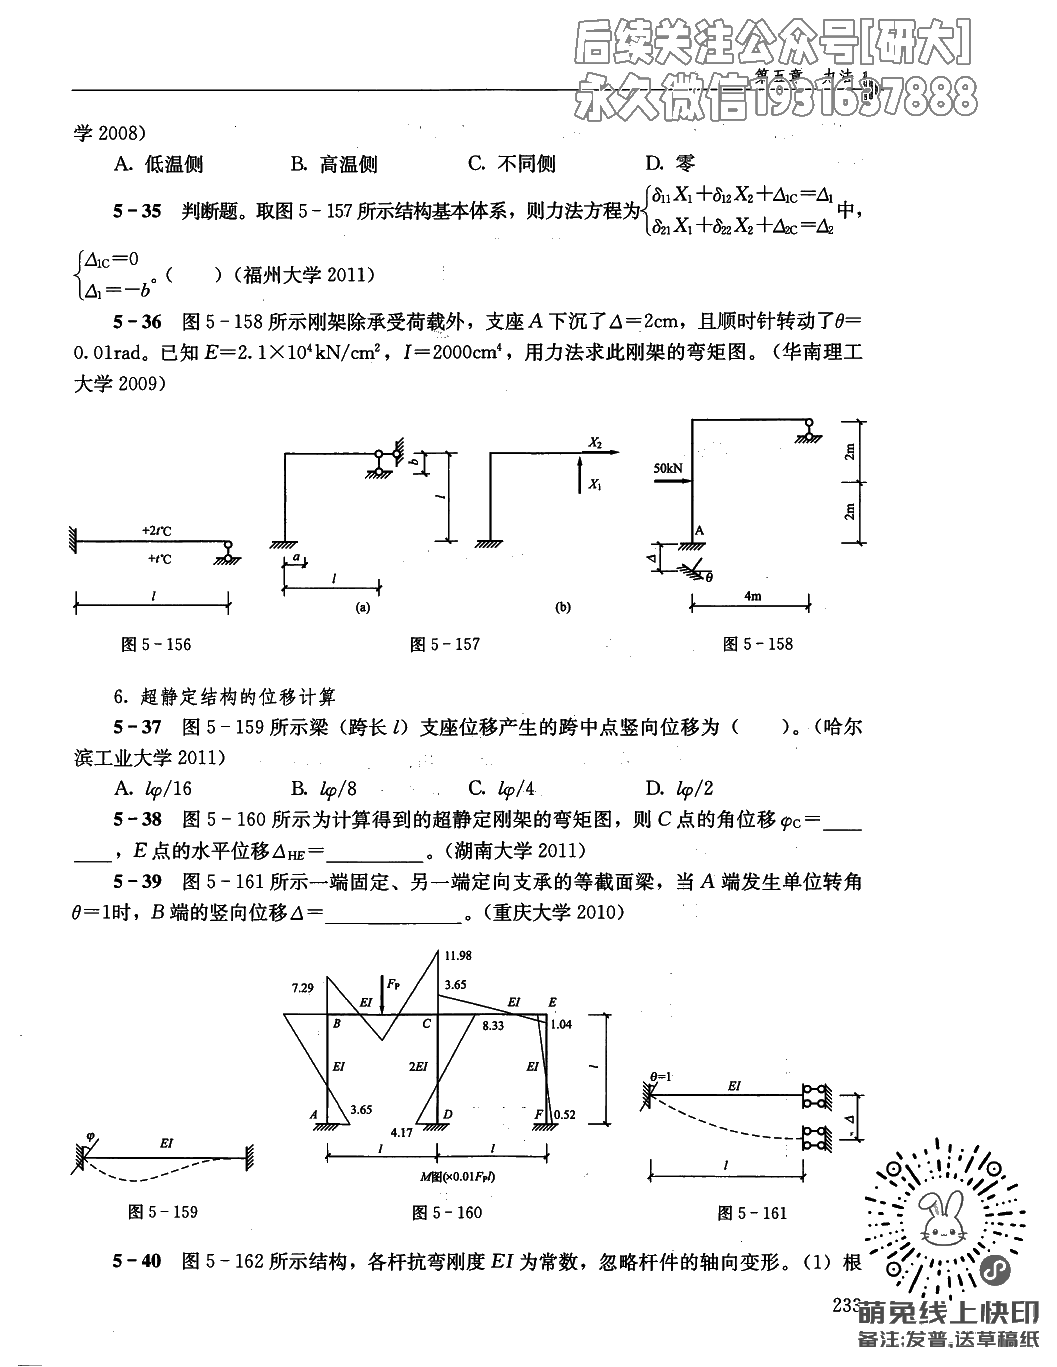
\includegraphics[width=0.96\textwidth,height=0.82\textheight,keepaspectratio]{images/c11_answer_1_p02.png}
\par\small 作业与答案（去水印版），第 2/8 页
\end{center}
\clearpage
\begin{center}
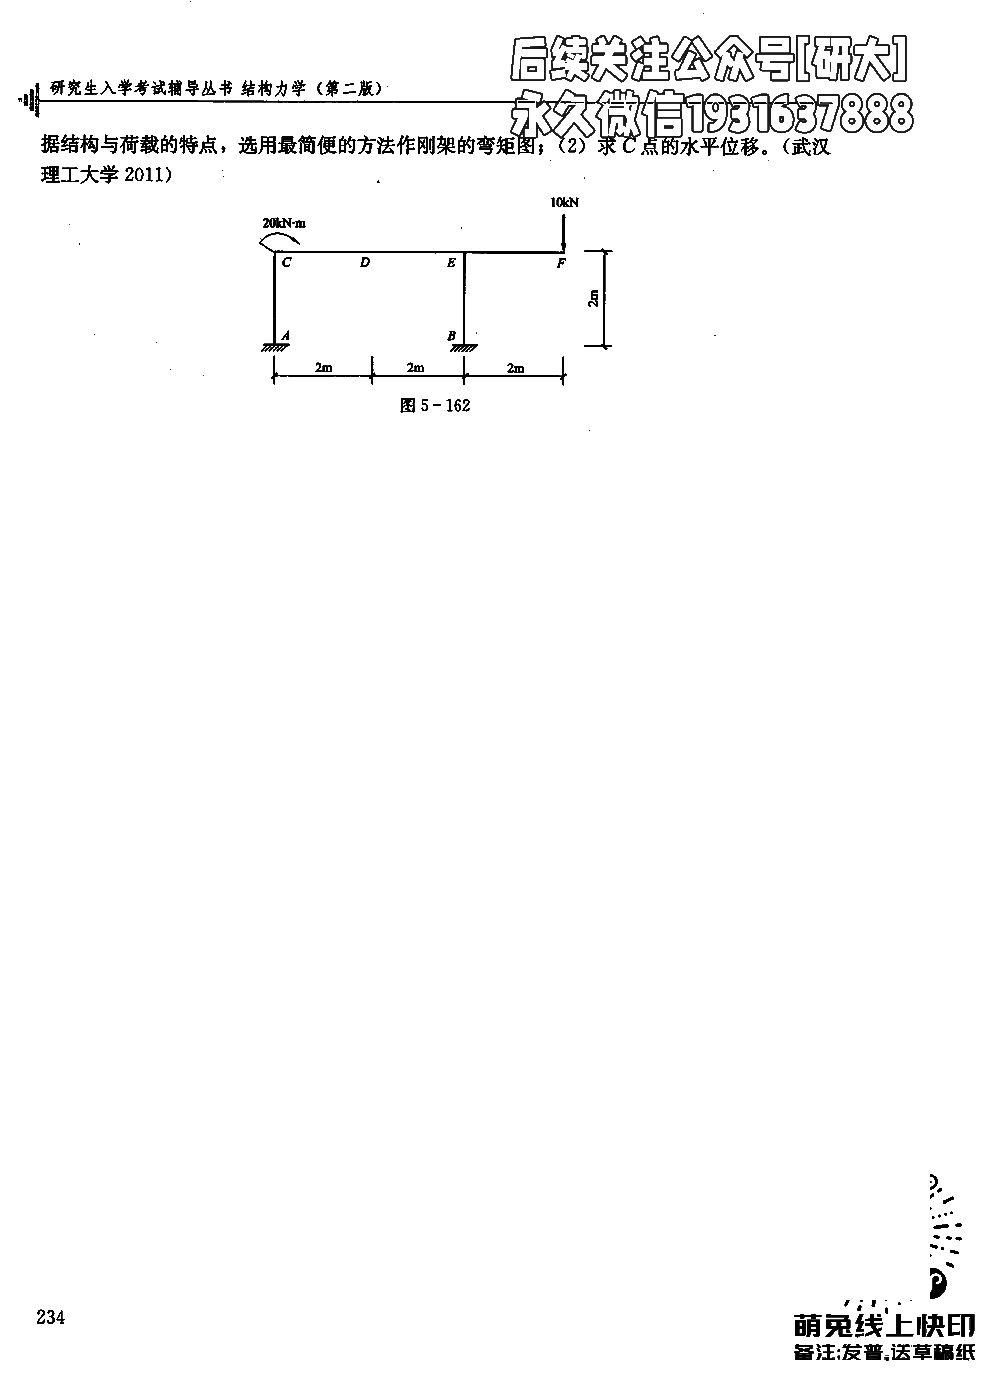
\includegraphics[width=0.96\textwidth,height=0.82\textheight,keepaspectratio]{images/c11_answer_1_p03.png}
\par\small 作业与答案（去水印版），第 3/8 页
\end{center}
\clearpage
\begin{center}
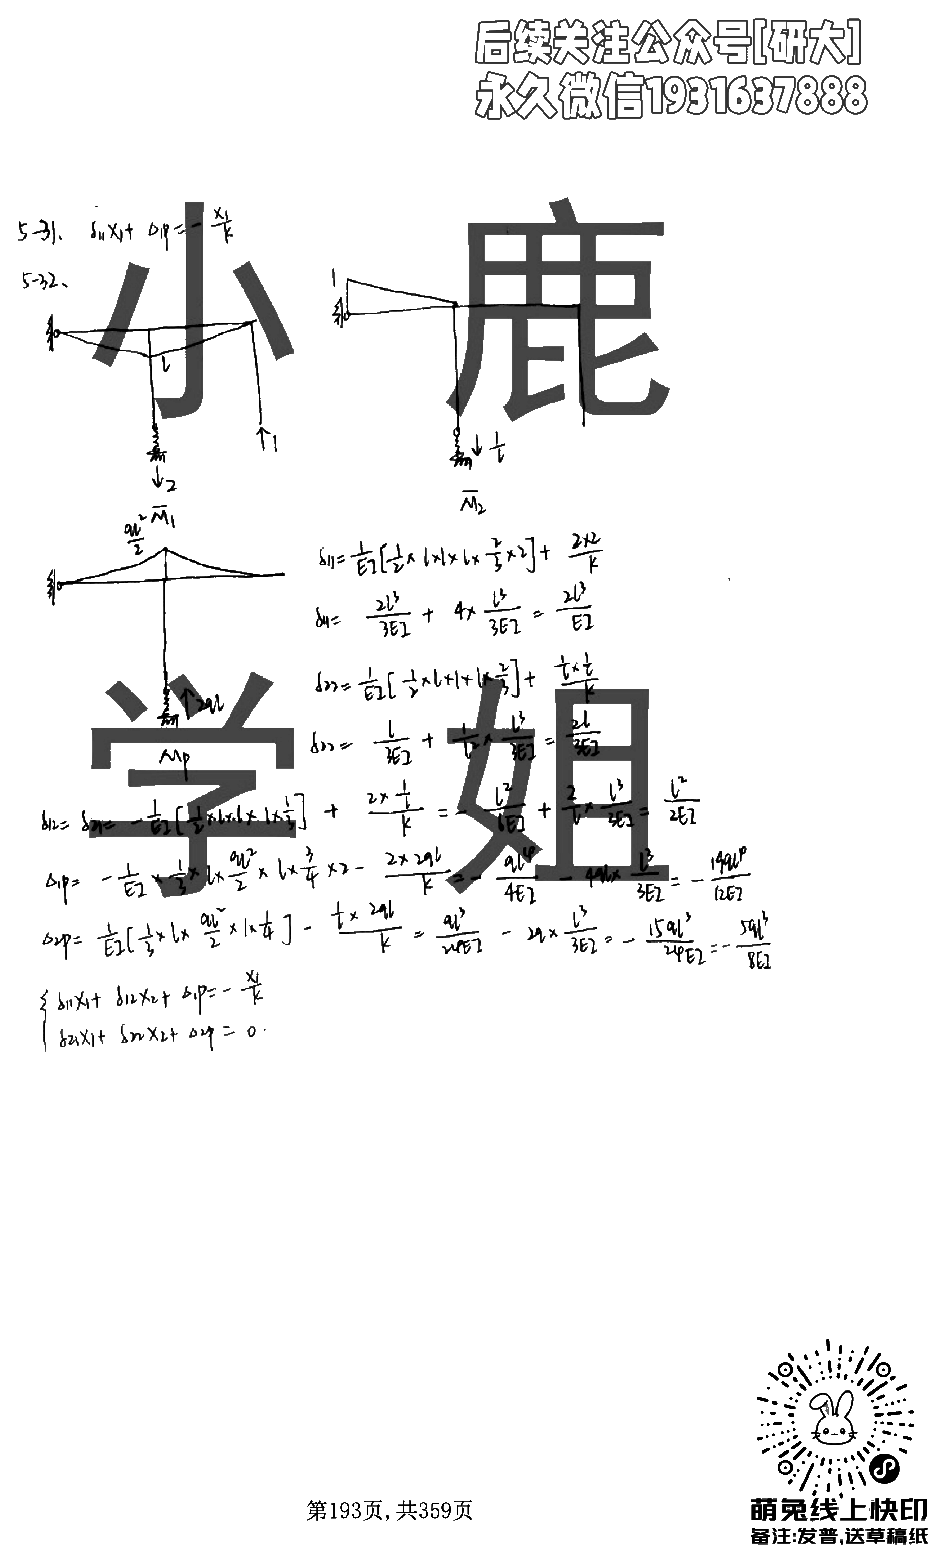
\includegraphics[width=0.96\textwidth,height=0.82\textheight,keepaspectratio]{images/c11_answer_1_p04.png}
\par\small 作业与答案（去水印版），第 4/8 页
\end{center}
\clearpage
\begin{center}
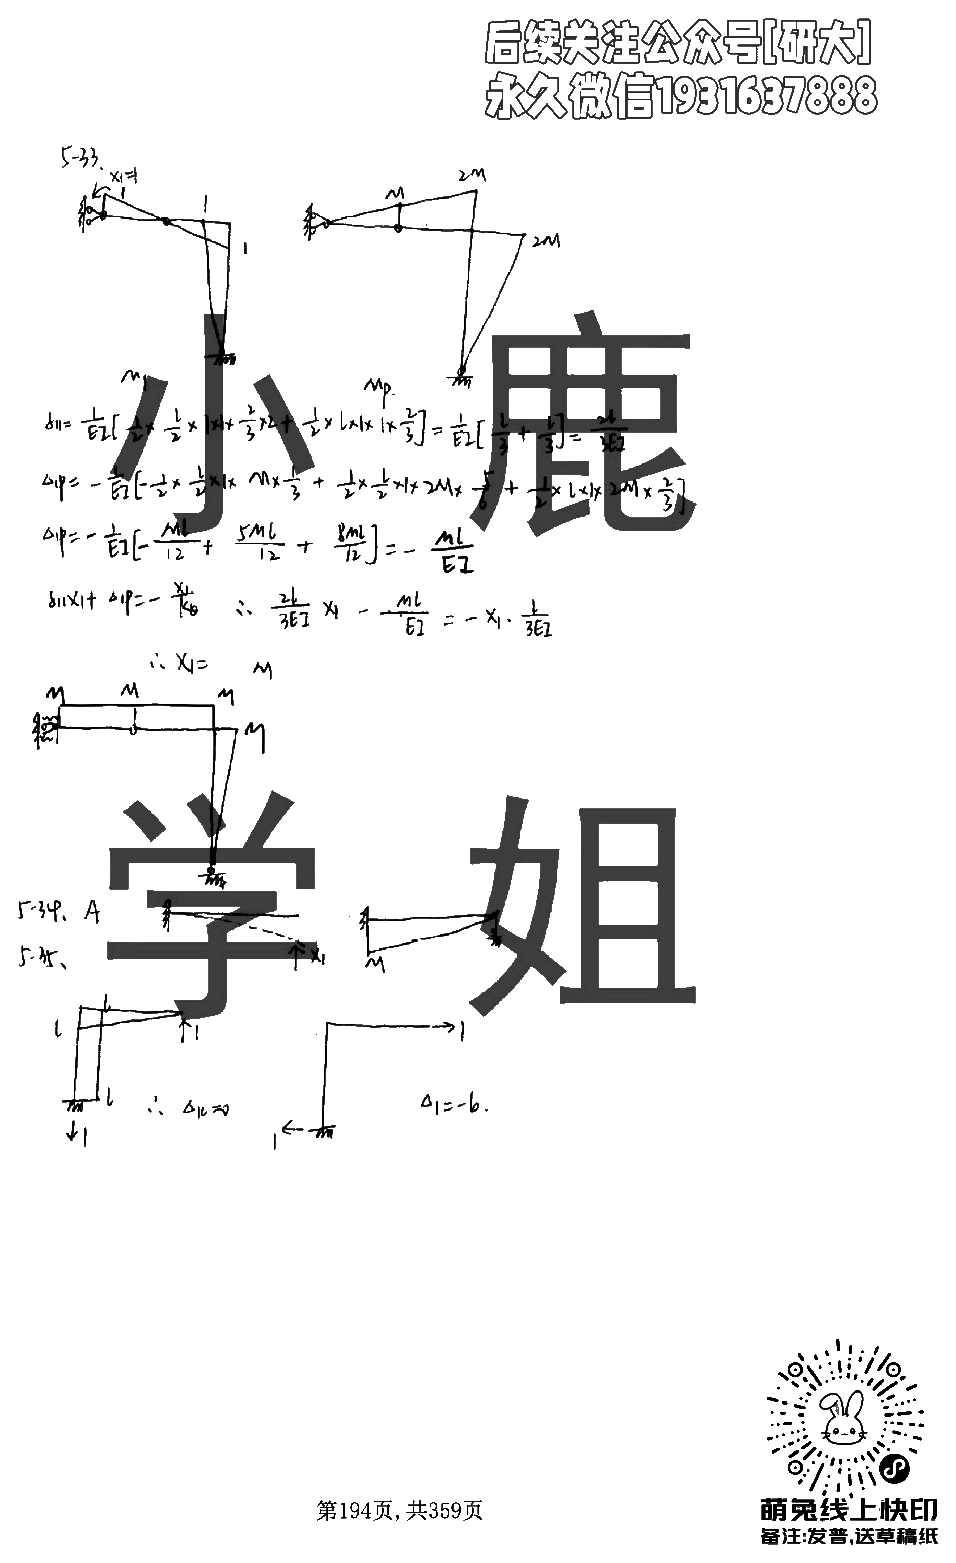
\includegraphics[width=0.96\textwidth,height=0.82\textheight,keepaspectratio]{images/c11_answer_1_p05.png}
\par\small 作业与答案（去水印版），第 5/8 页
\end{center}
\clearpage
\begin{center}
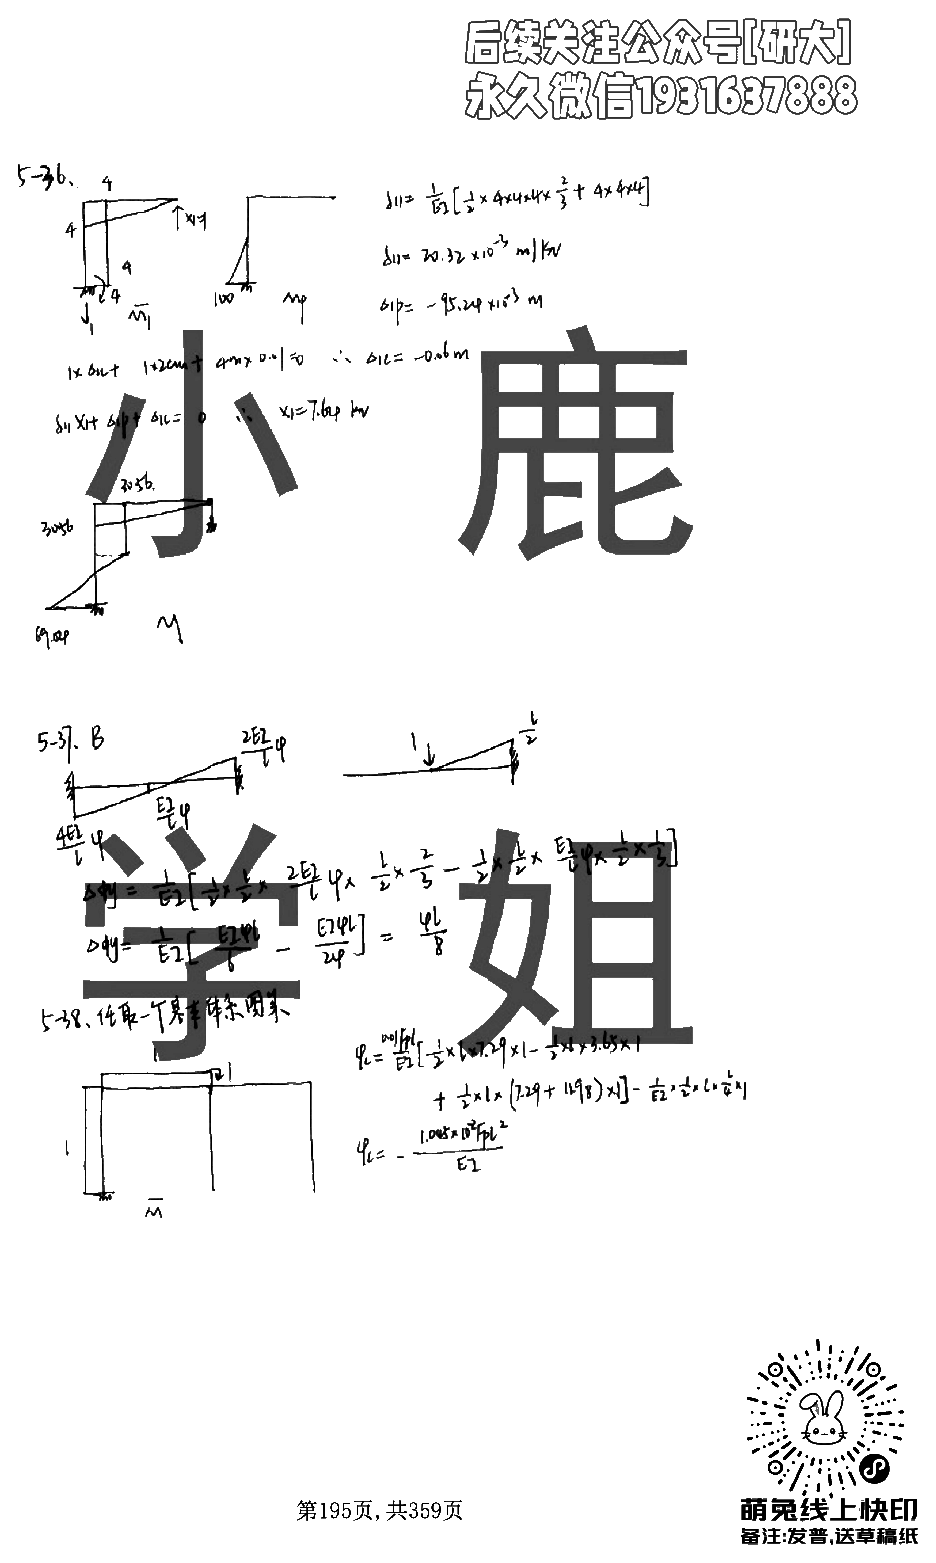
\includegraphics[width=0.96\textwidth,height=0.82\textheight,keepaspectratio]{images/c11_answer_1_p06.png}
\par\small 作业与答案（去水印版），第 6/8 页
\end{center}
\clearpage
\begin{center}
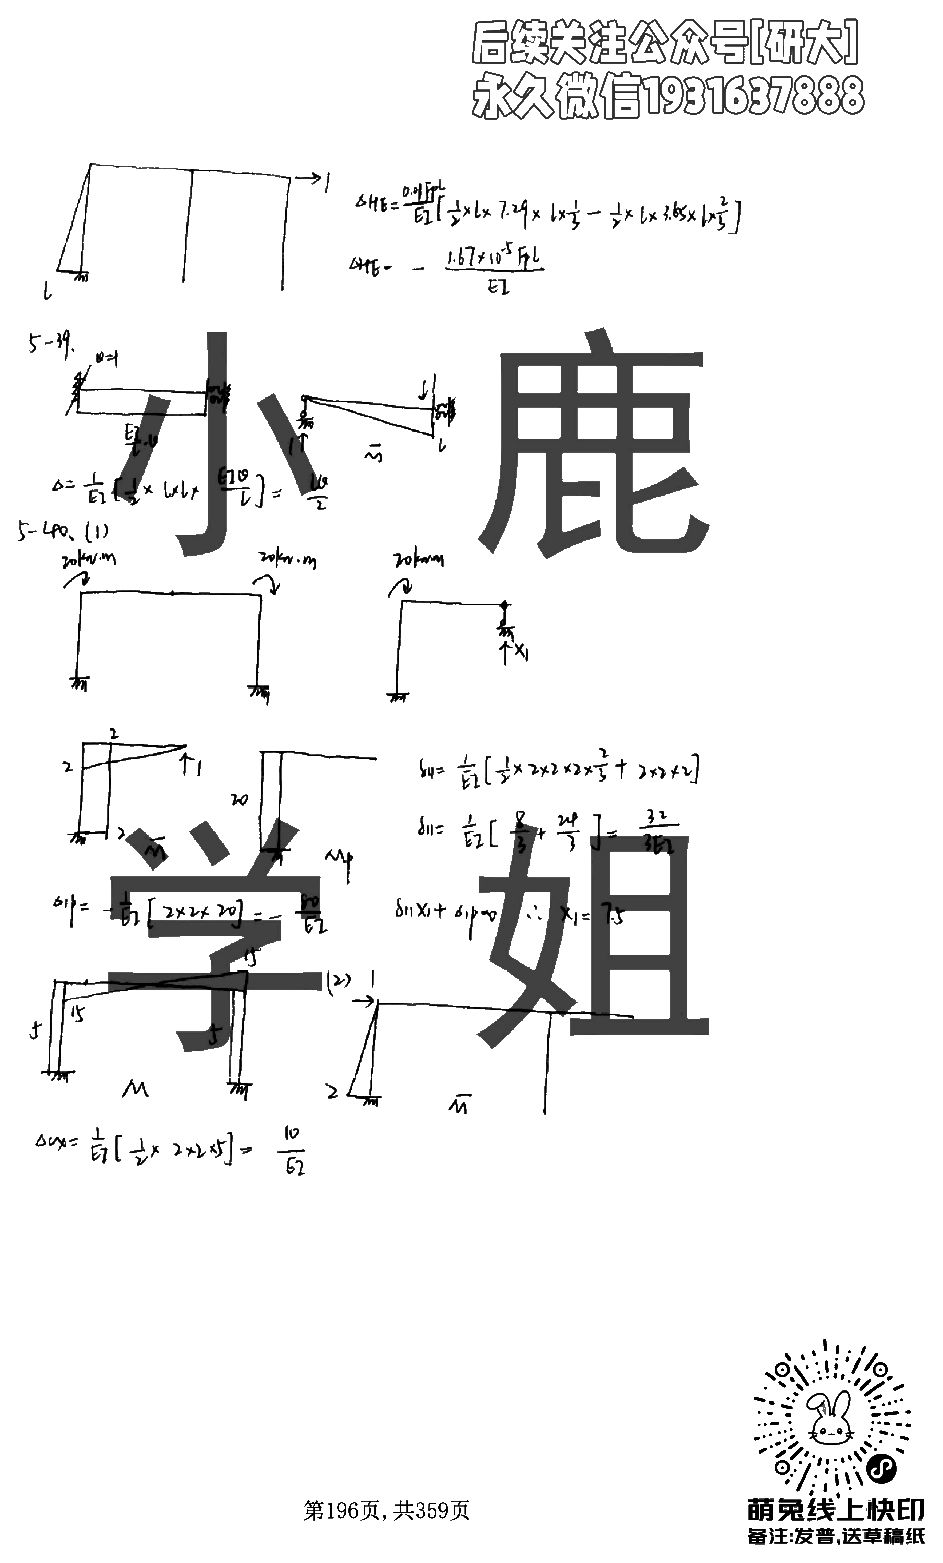
\includegraphics[width=0.96\textwidth,height=0.82\textheight,keepaspectratio]{images/c11_answer_1_p07.png}
\par\small 作业与答案（去水印版），第 7/8 页
\end{center}
\clearpage
\begin{center}
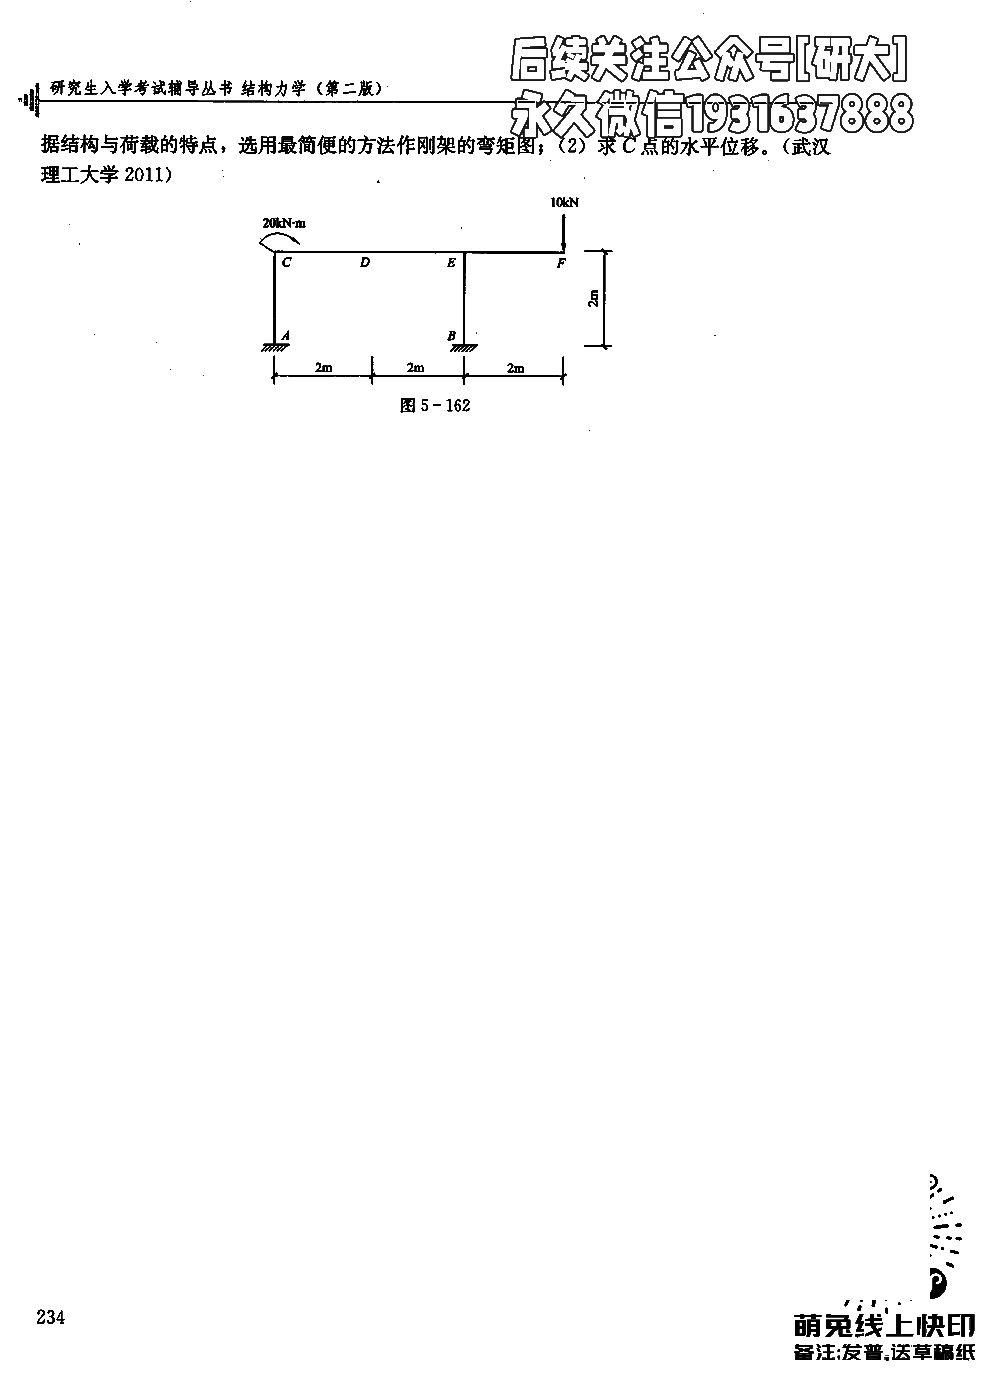
\includegraphics[width=0.96\textwidth,height=0.82\textheight,keepaspectratio]{images/c11_answer_1_p08.png}
\par\small 作业与答案（去水印版），第 8/8 页
\end{center}
\clearpage
\section{讲解笔记（去水印版）}
\begin{center}
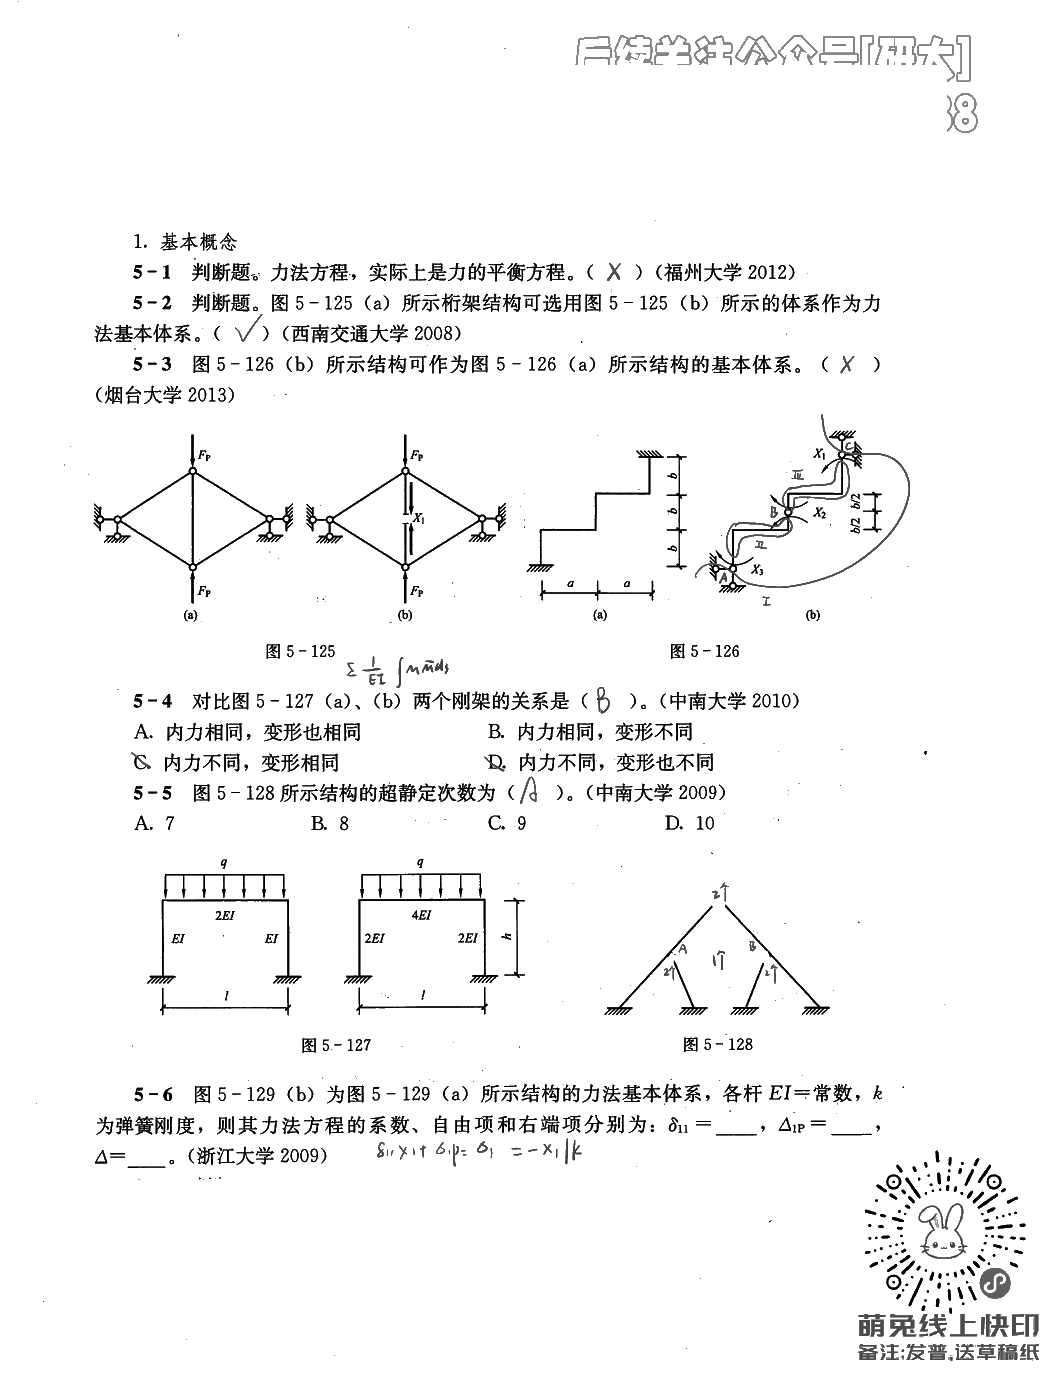
\includegraphics[width=0.96\textwidth,height=0.82\textheight,keepaspectratio]{images/c11_note_p01.png}
\par\small 讲解笔记（去水印版），第 1/21 页
\end{center}
\clearpage
\begin{center}
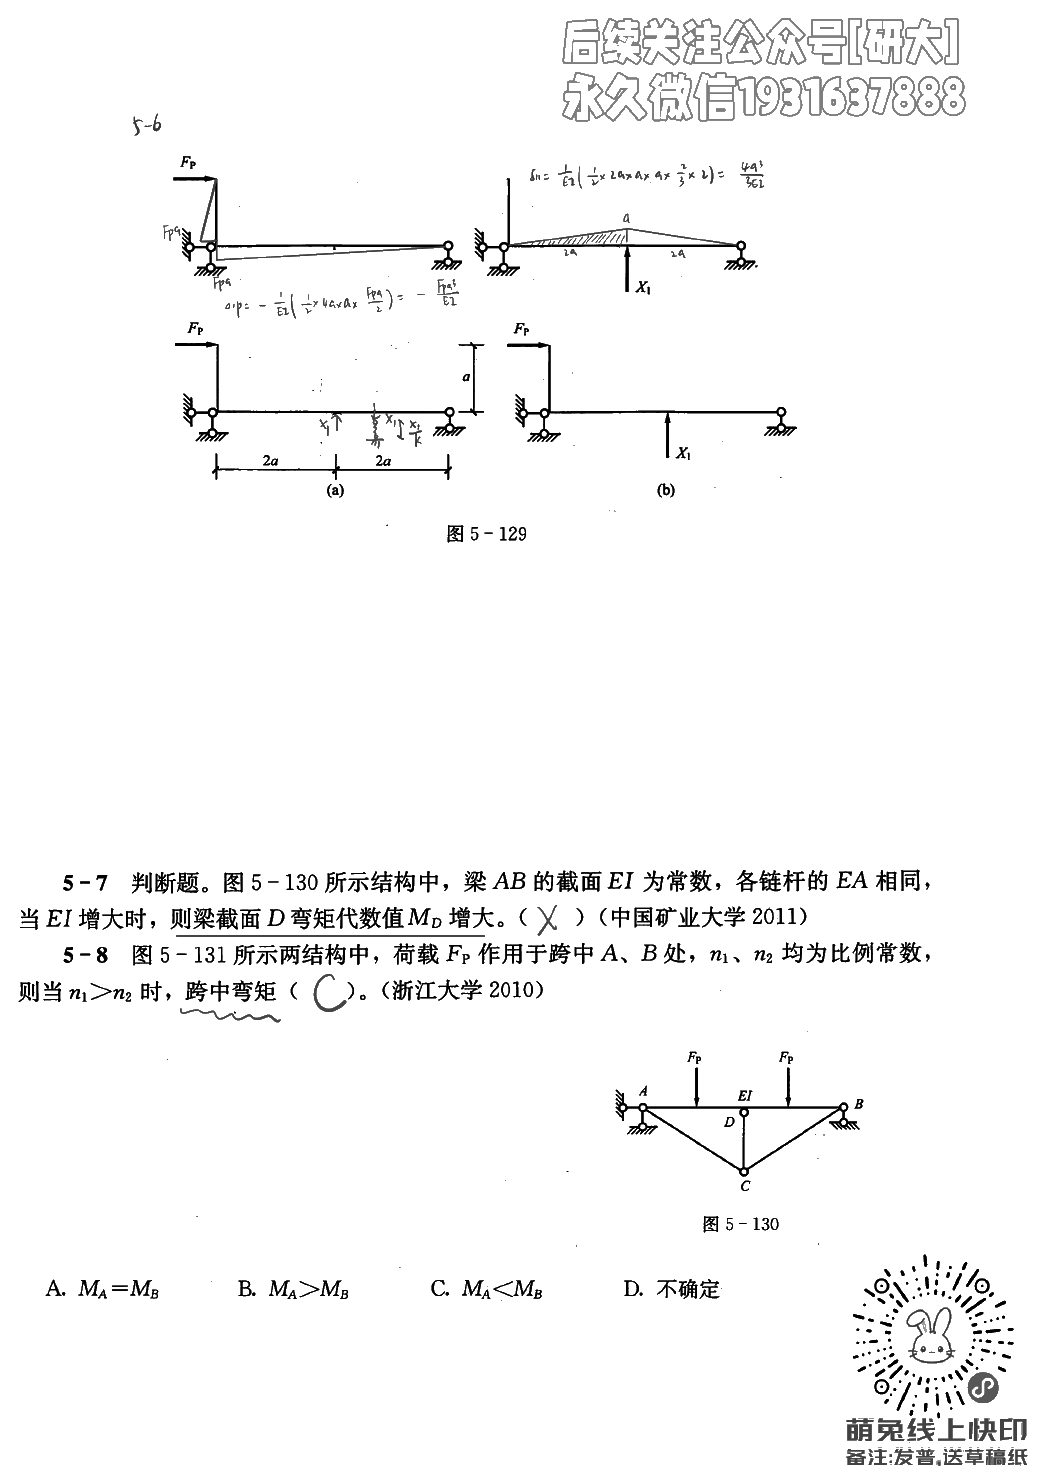
\includegraphics[width=0.96\textwidth,height=0.82\textheight,keepaspectratio]{images/c11_note_p02.png}
\par\small 讲解笔记（去水印版），第 2/21 页
\end{center}
\clearpage
\begin{center}
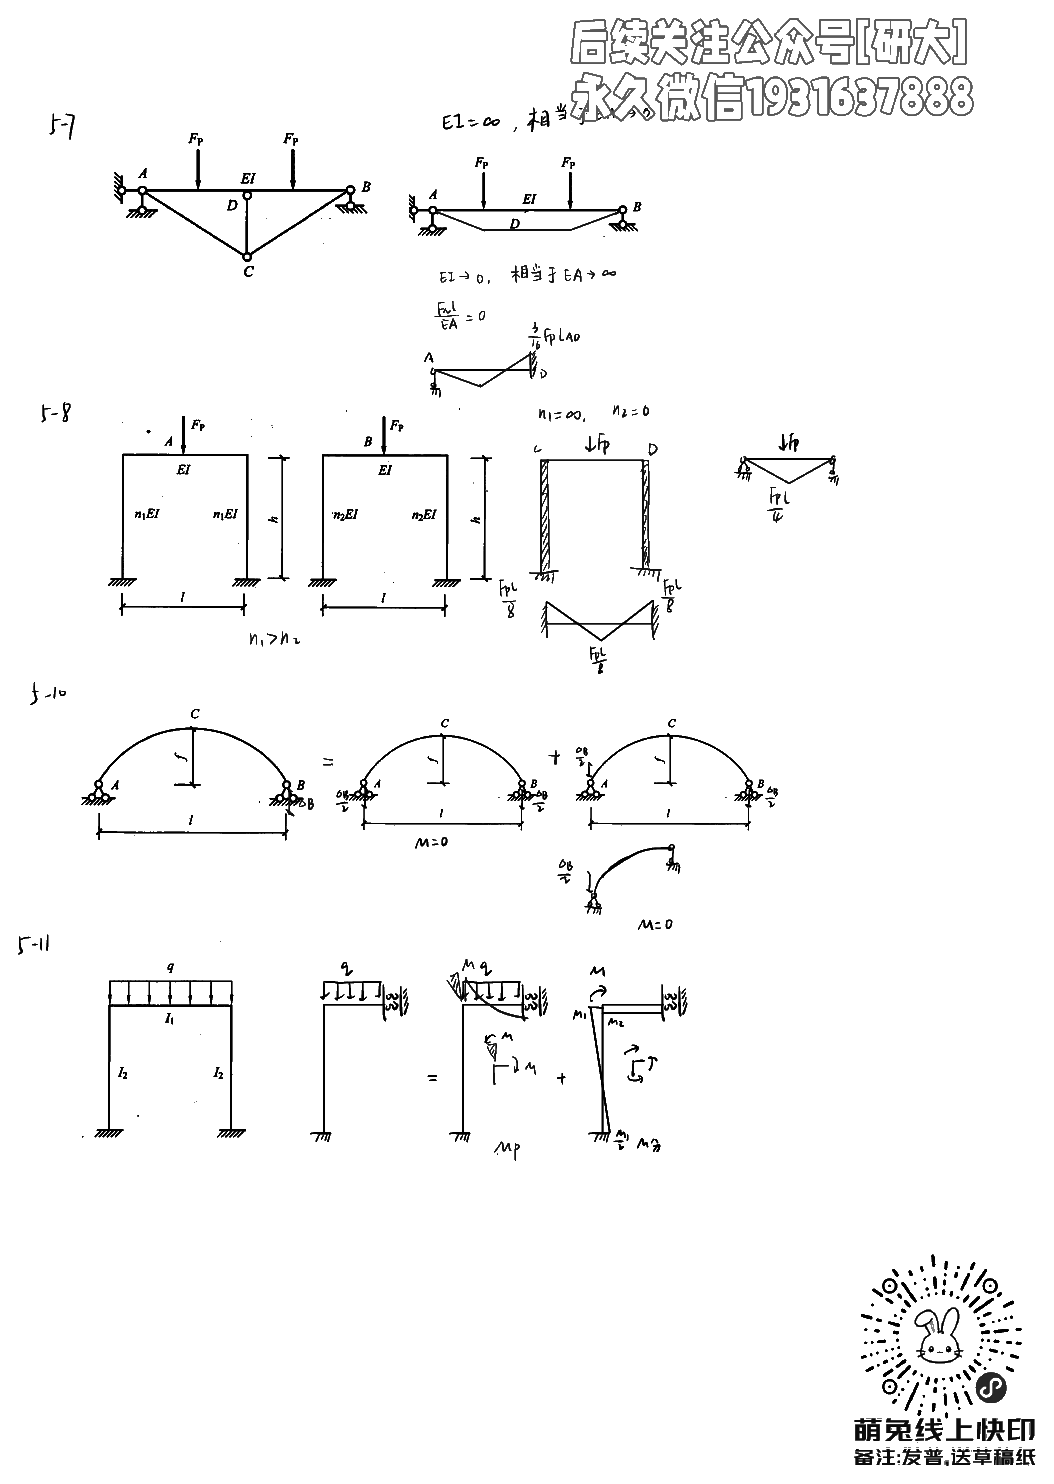
\includegraphics[width=0.96\textwidth,height=0.82\textheight,keepaspectratio]{images/c11_note_p03.png}
\par\small 讲解笔记（去水印版），第 3/21 页
\end{center}
\clearpage
\begin{center}
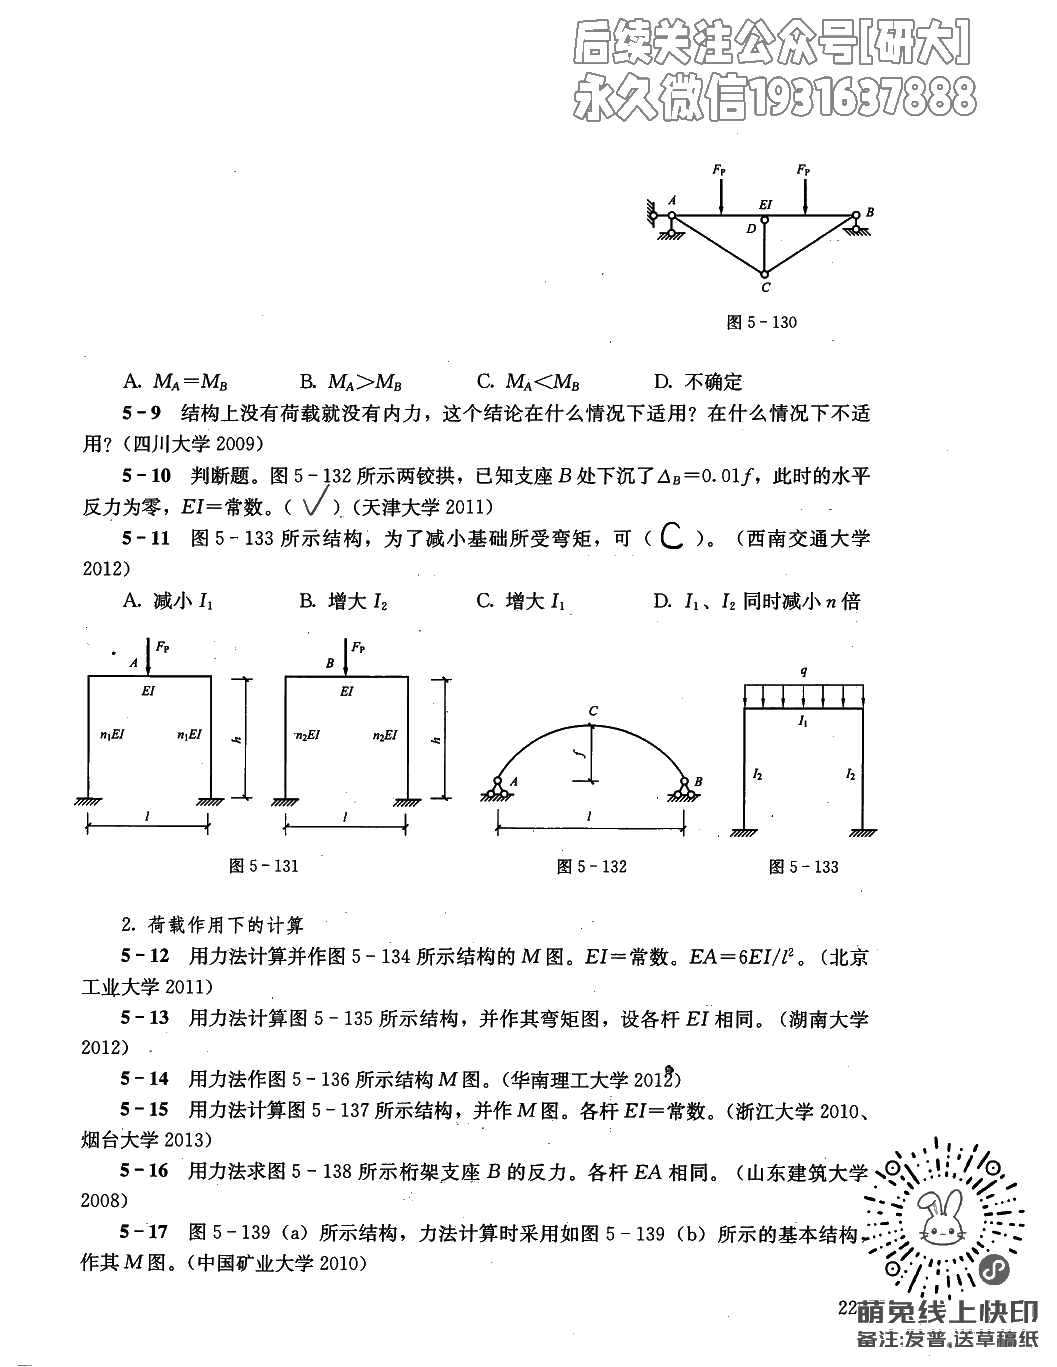
\includegraphics[width=0.96\textwidth,height=0.82\textheight,keepaspectratio]{images/c11_note_p04.png}
\par\small 讲解笔记（去水印版），第 4/21 页
\end{center}
\clearpage
\begin{center}
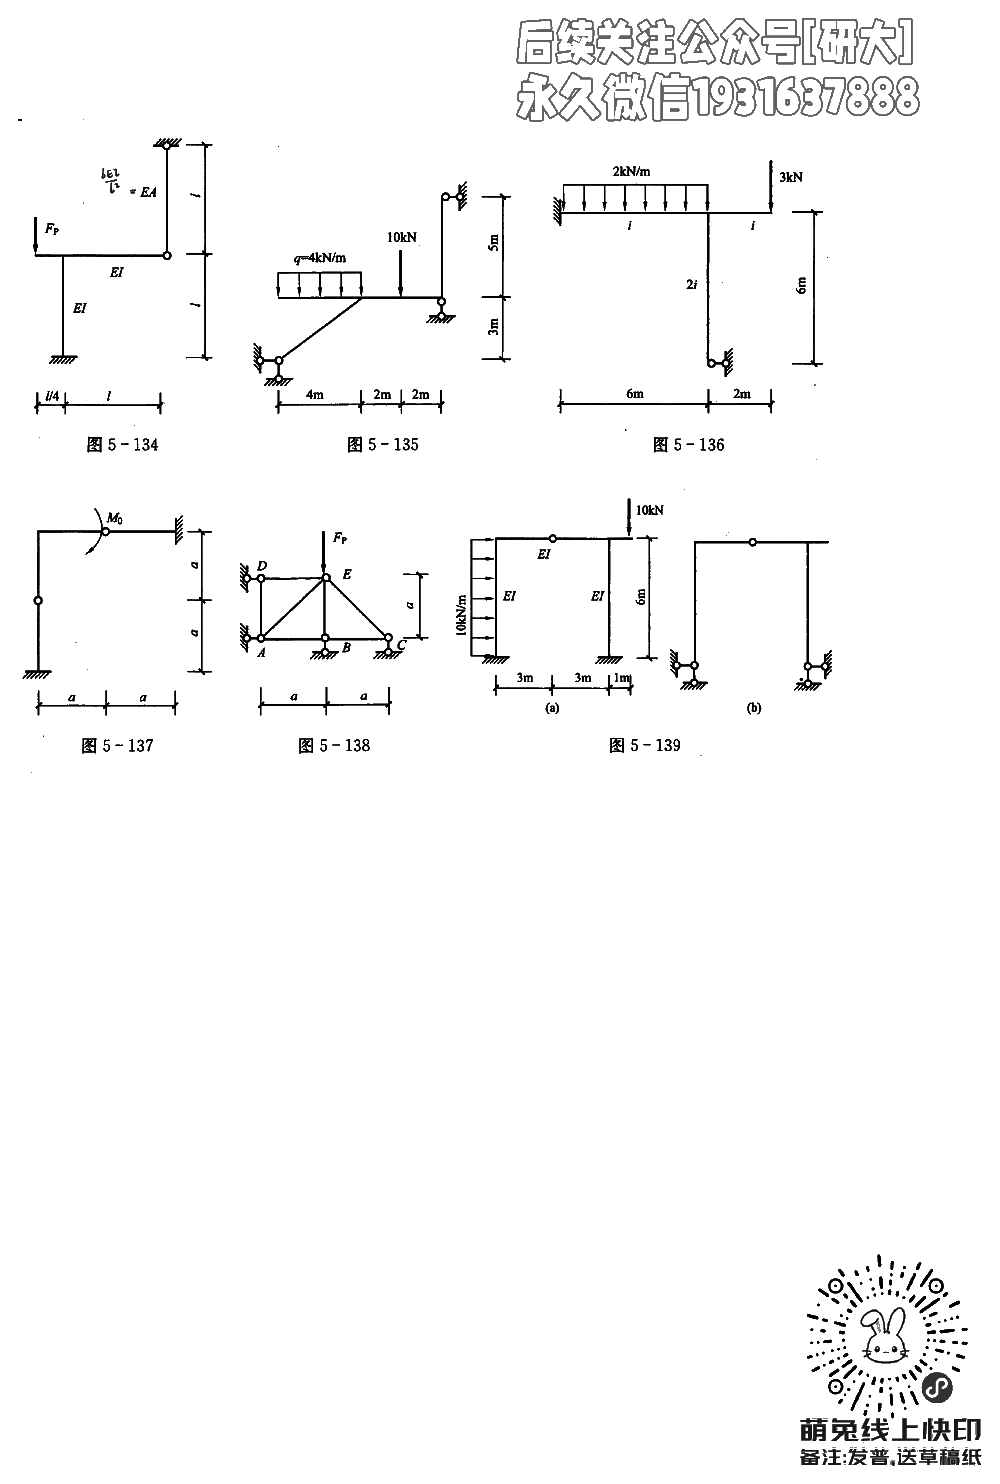
\includegraphics[width=0.96\textwidth,height=0.82\textheight,keepaspectratio]{images/c11_note_p05.png}
\par\small 讲解笔记（去水印版），第 5/21 页
\end{center}
\clearpage
\begin{center}
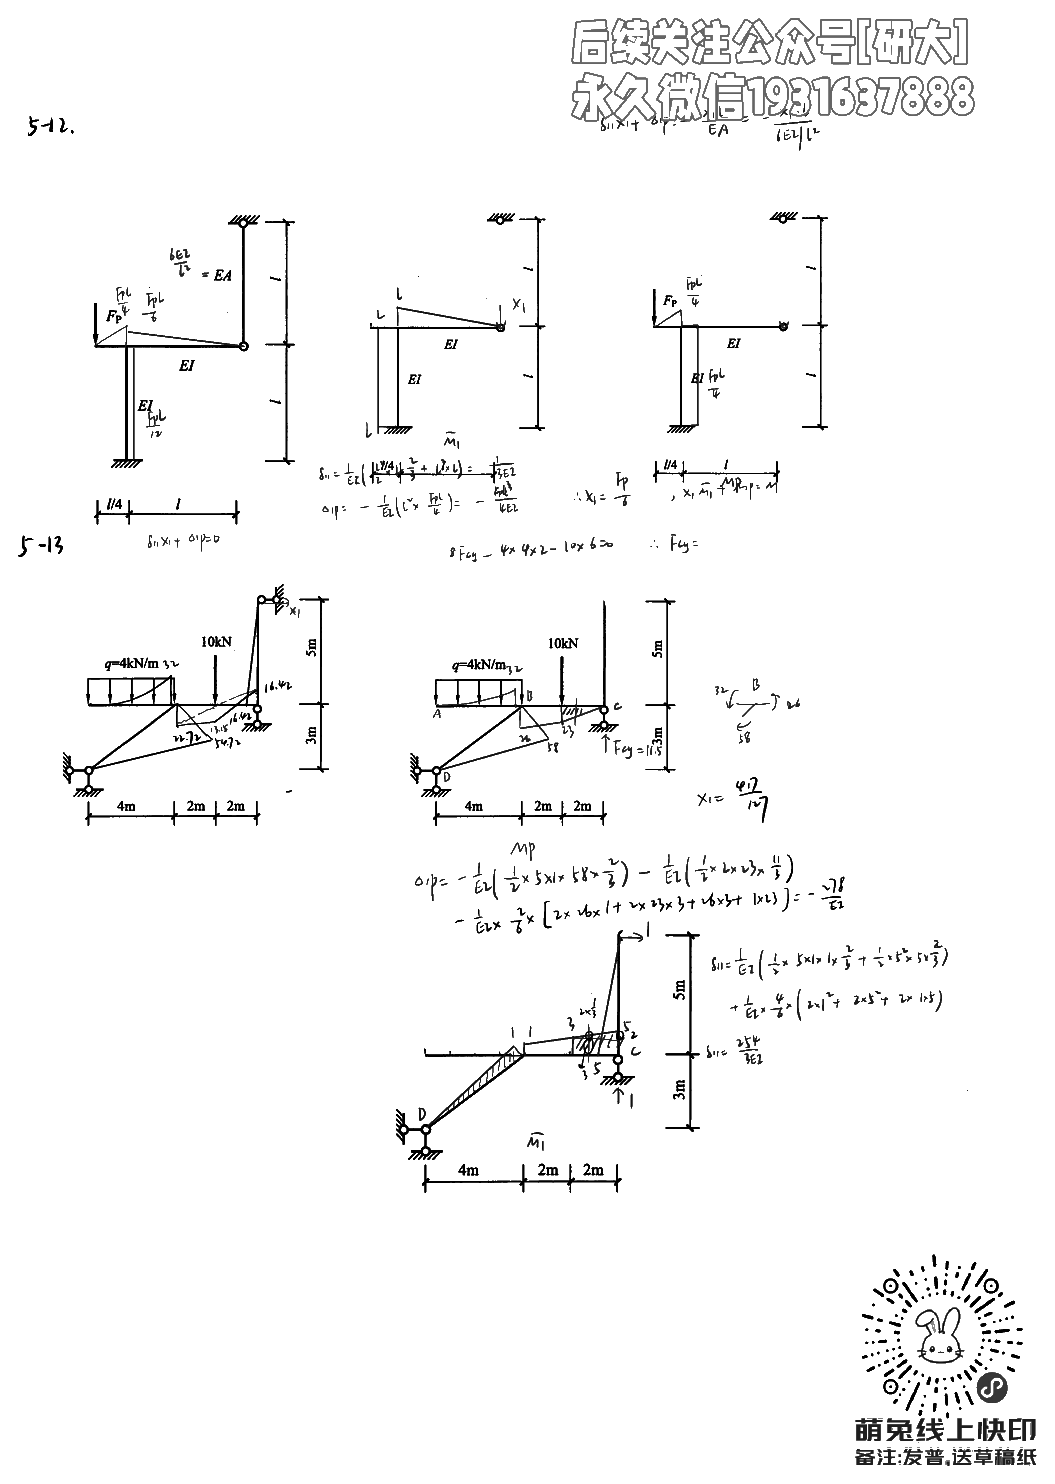
\includegraphics[width=0.96\textwidth,height=0.82\textheight,keepaspectratio]{images/c11_note_p06.png}
\par\small 讲解笔记（去水印版），第 6/21 页
\end{center}
\clearpage
\begin{center}
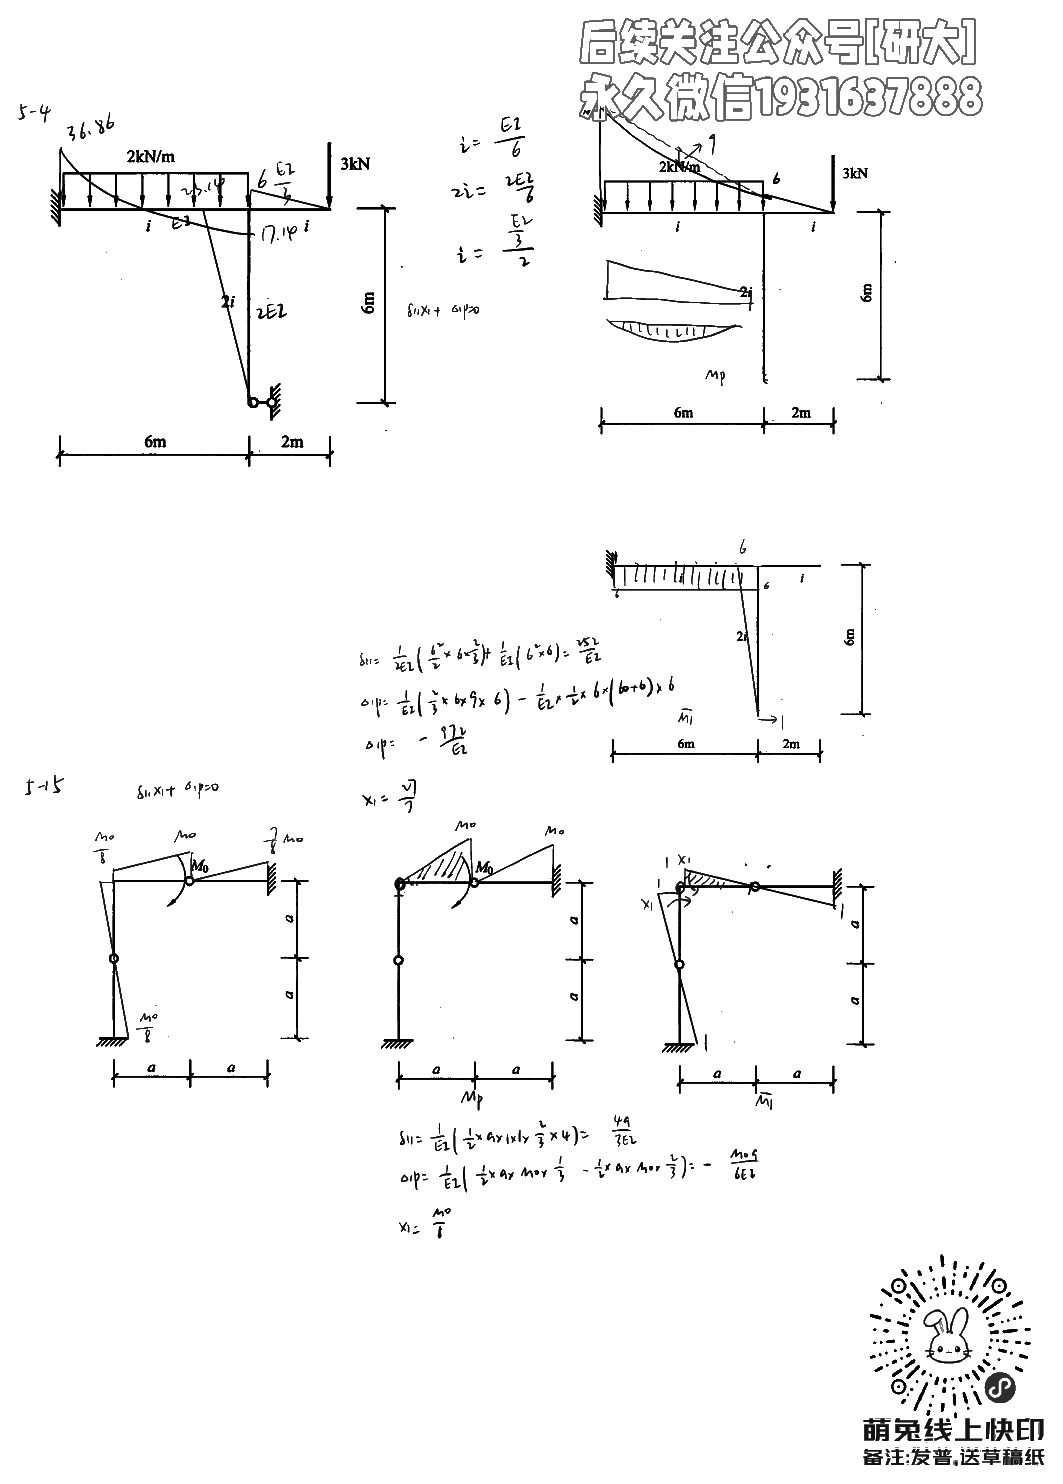
\includegraphics[width=0.96\textwidth,height=0.82\textheight,keepaspectratio]{images/c11_note_p07.png}
\par\small 讲解笔记（去水印版），第 7/21 页
\end{center}
\clearpage
\begin{center}
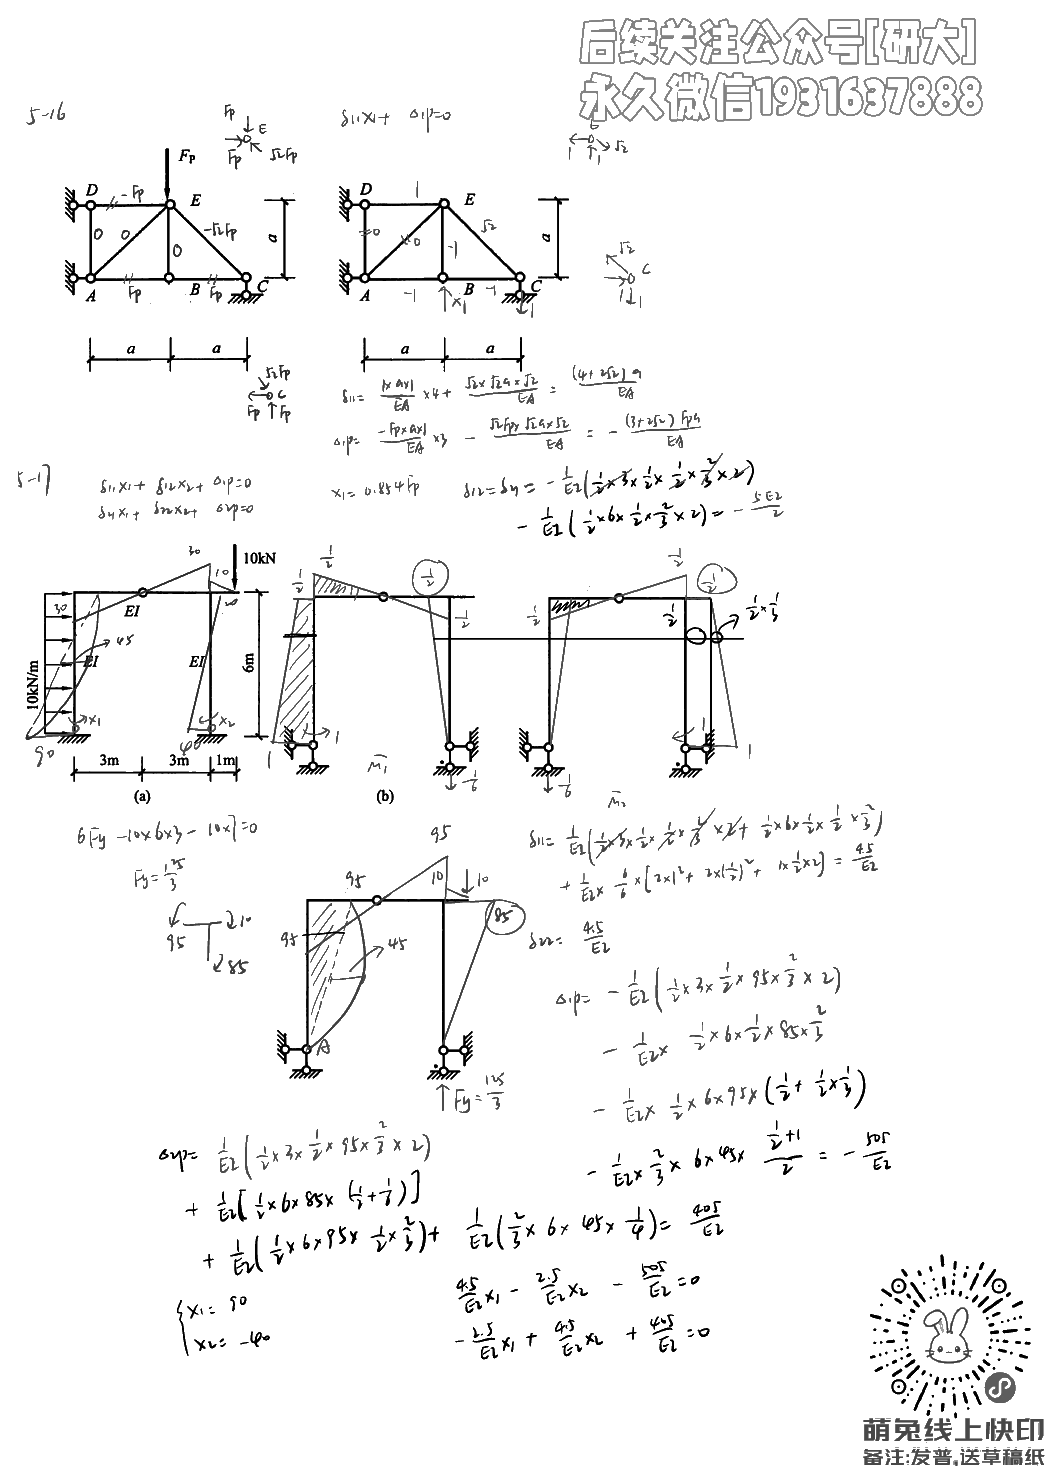
\includegraphics[width=0.96\textwidth,height=0.82\textheight,keepaspectratio]{images/c11_note_p08.png}
\par\small 讲解笔记（去水印版），第 8/21 页
\end{center}
\clearpage
\begin{center}
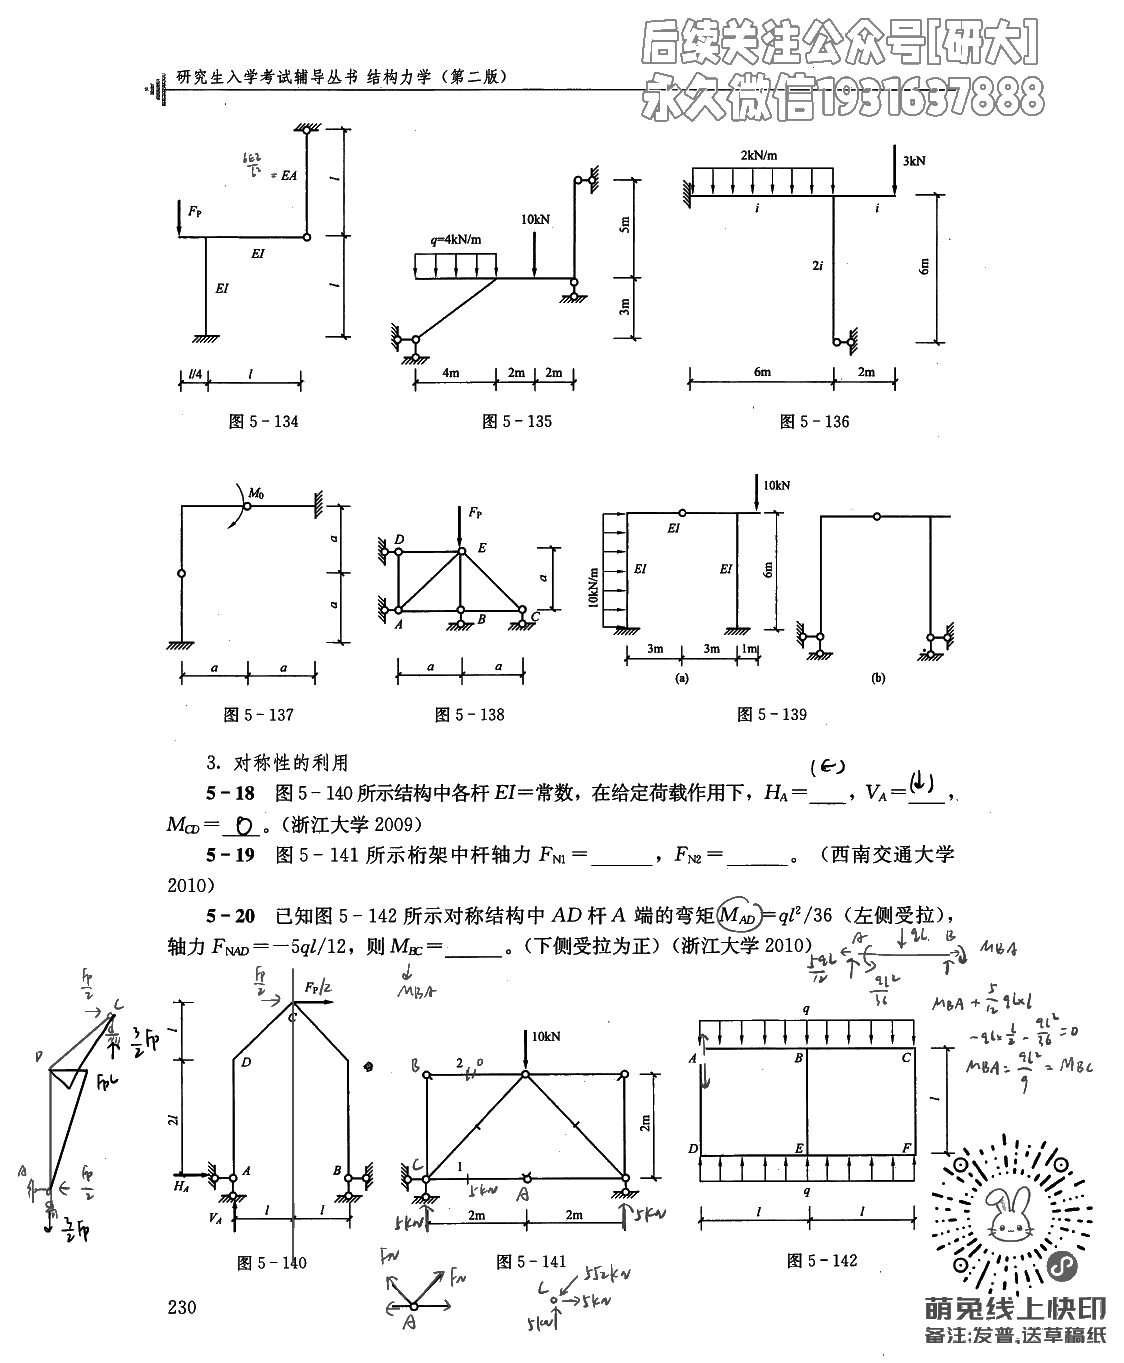
\includegraphics[width=0.96\textwidth,height=0.82\textheight,keepaspectratio]{images/c11_note_p09.png}
\par\small 讲解笔记（去水印版），第 9/21 页
\end{center}
\clearpage
\begin{center}
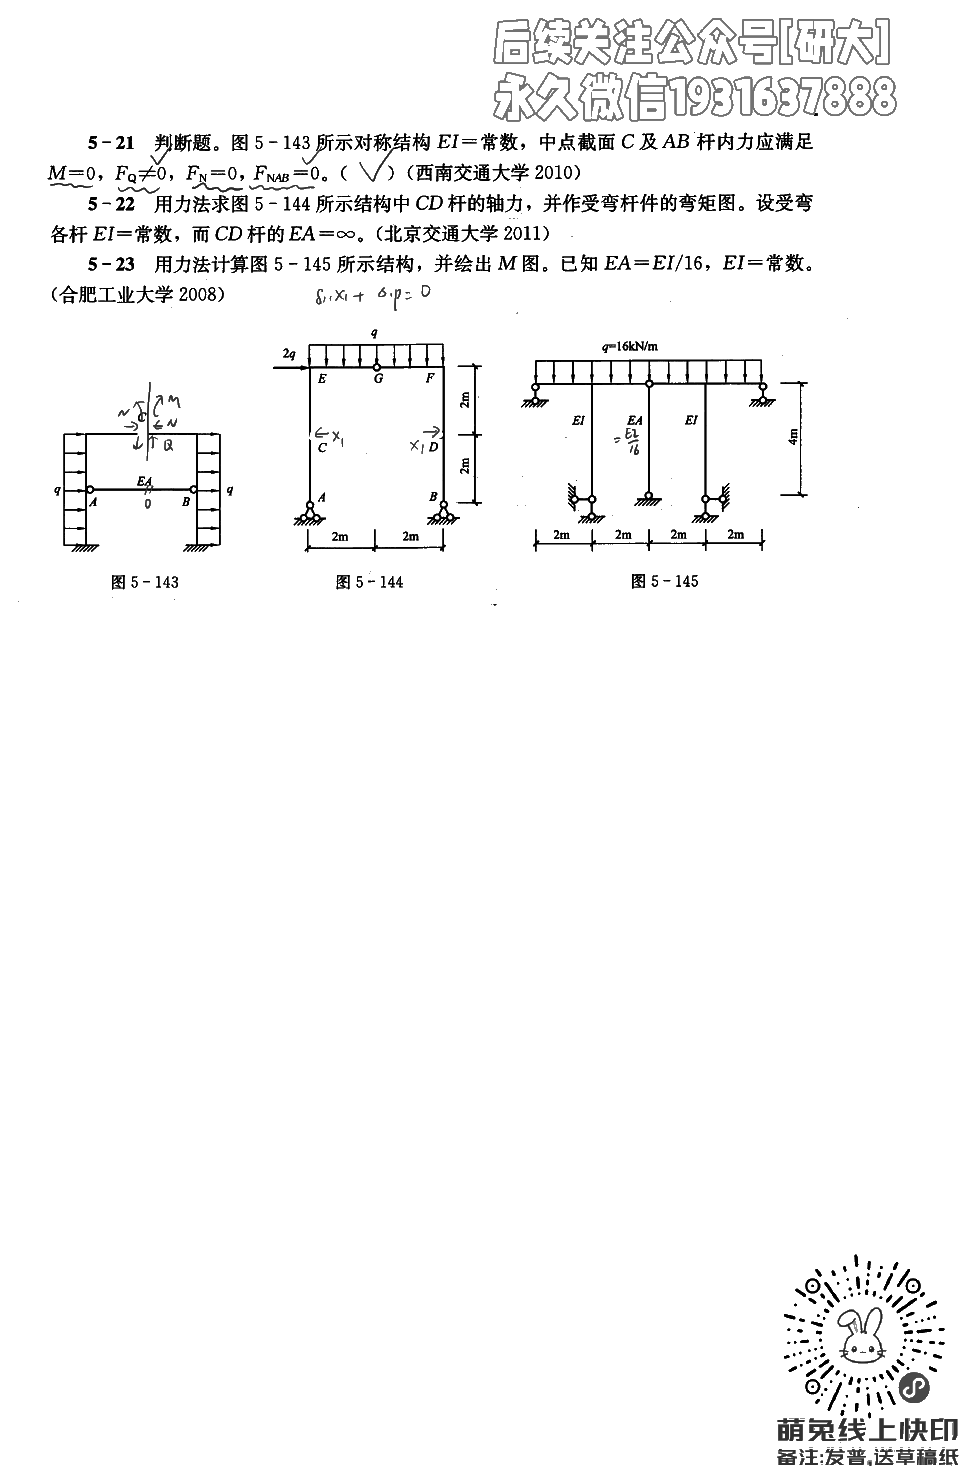
\includegraphics[width=0.96\textwidth,height=0.82\textheight,keepaspectratio]{images/c11_note_p10.png}
\par\small 讲解笔记（去水印版），第 10/21 页
\end{center}
\clearpage
\begin{center}
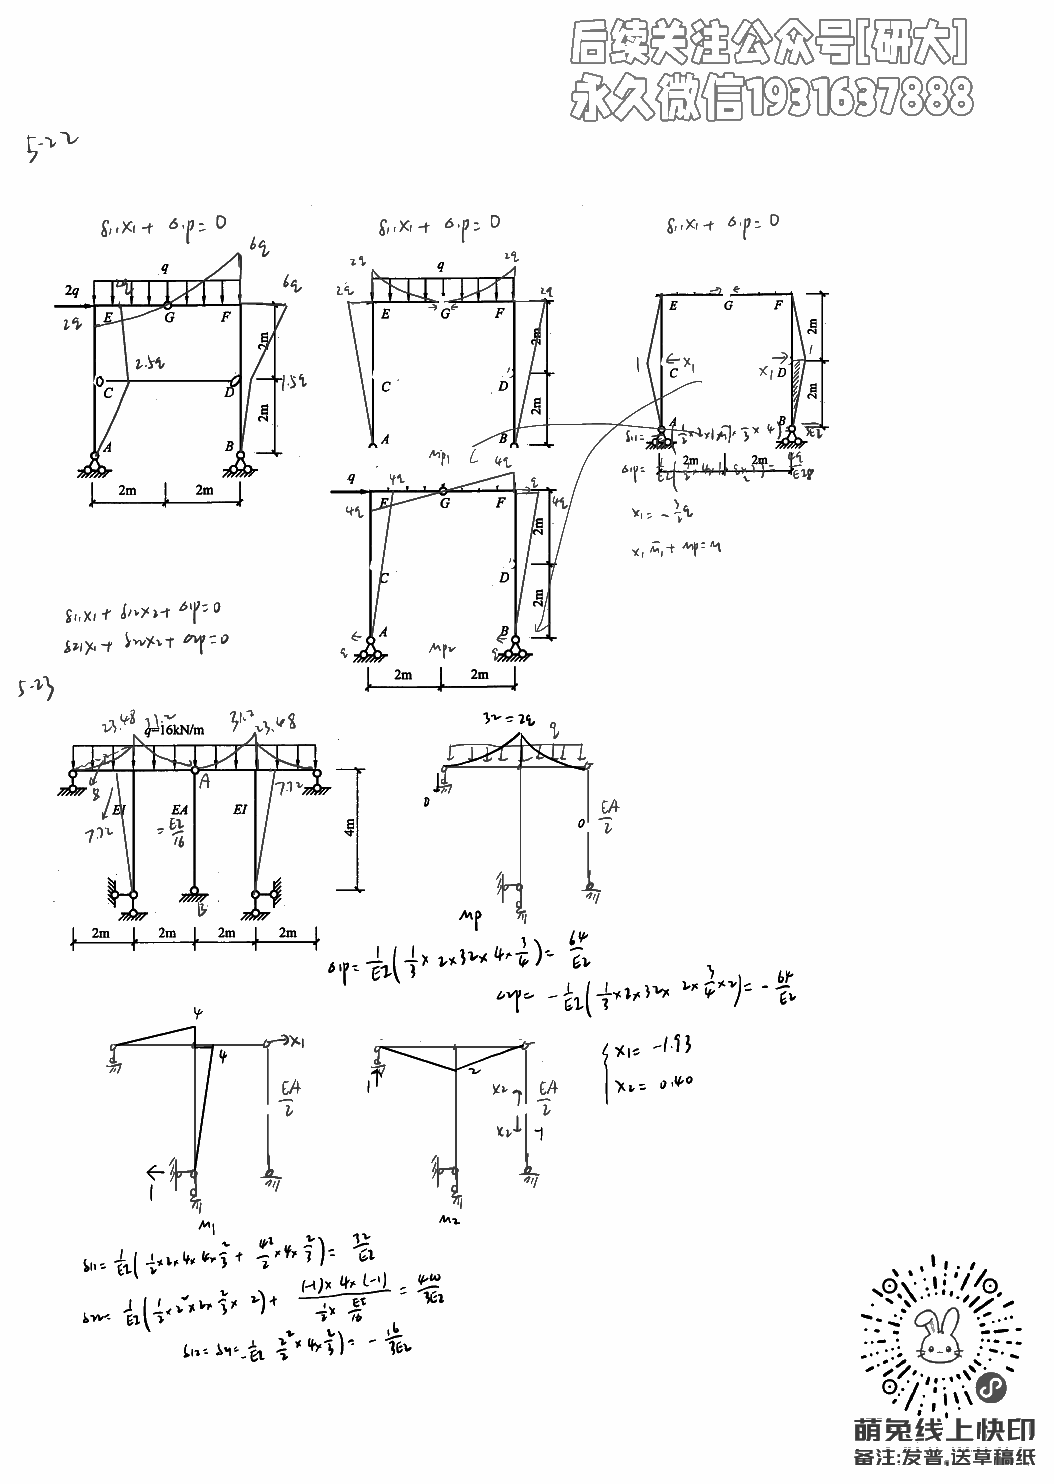
\includegraphics[width=0.96\textwidth,height=0.82\textheight,keepaspectratio]{images/c11_note_p11.png}
\par\small 讲解笔记（去水印版），第 11/21 页
\end{center}
\clearpage
\begin{center}
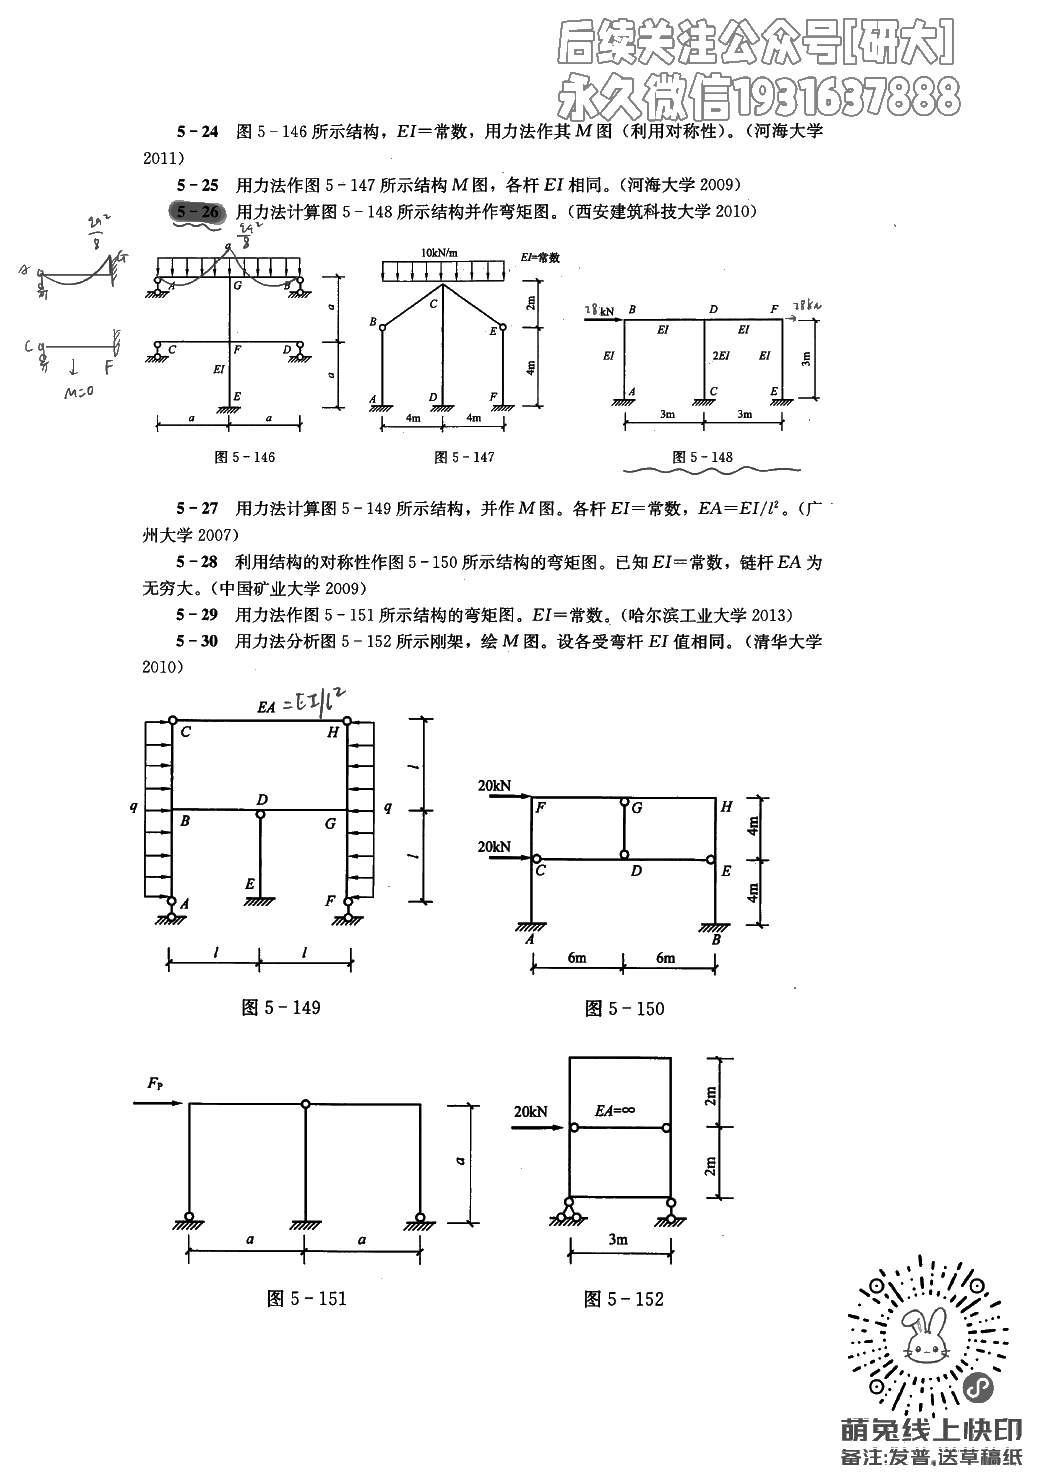
\includegraphics[width=0.96\textwidth,height=0.82\textheight,keepaspectratio]{images/c11_note_p12.png}
\par\small 讲解笔记（去水印版），第 12/21 页
\end{center}
\clearpage
\begin{center}
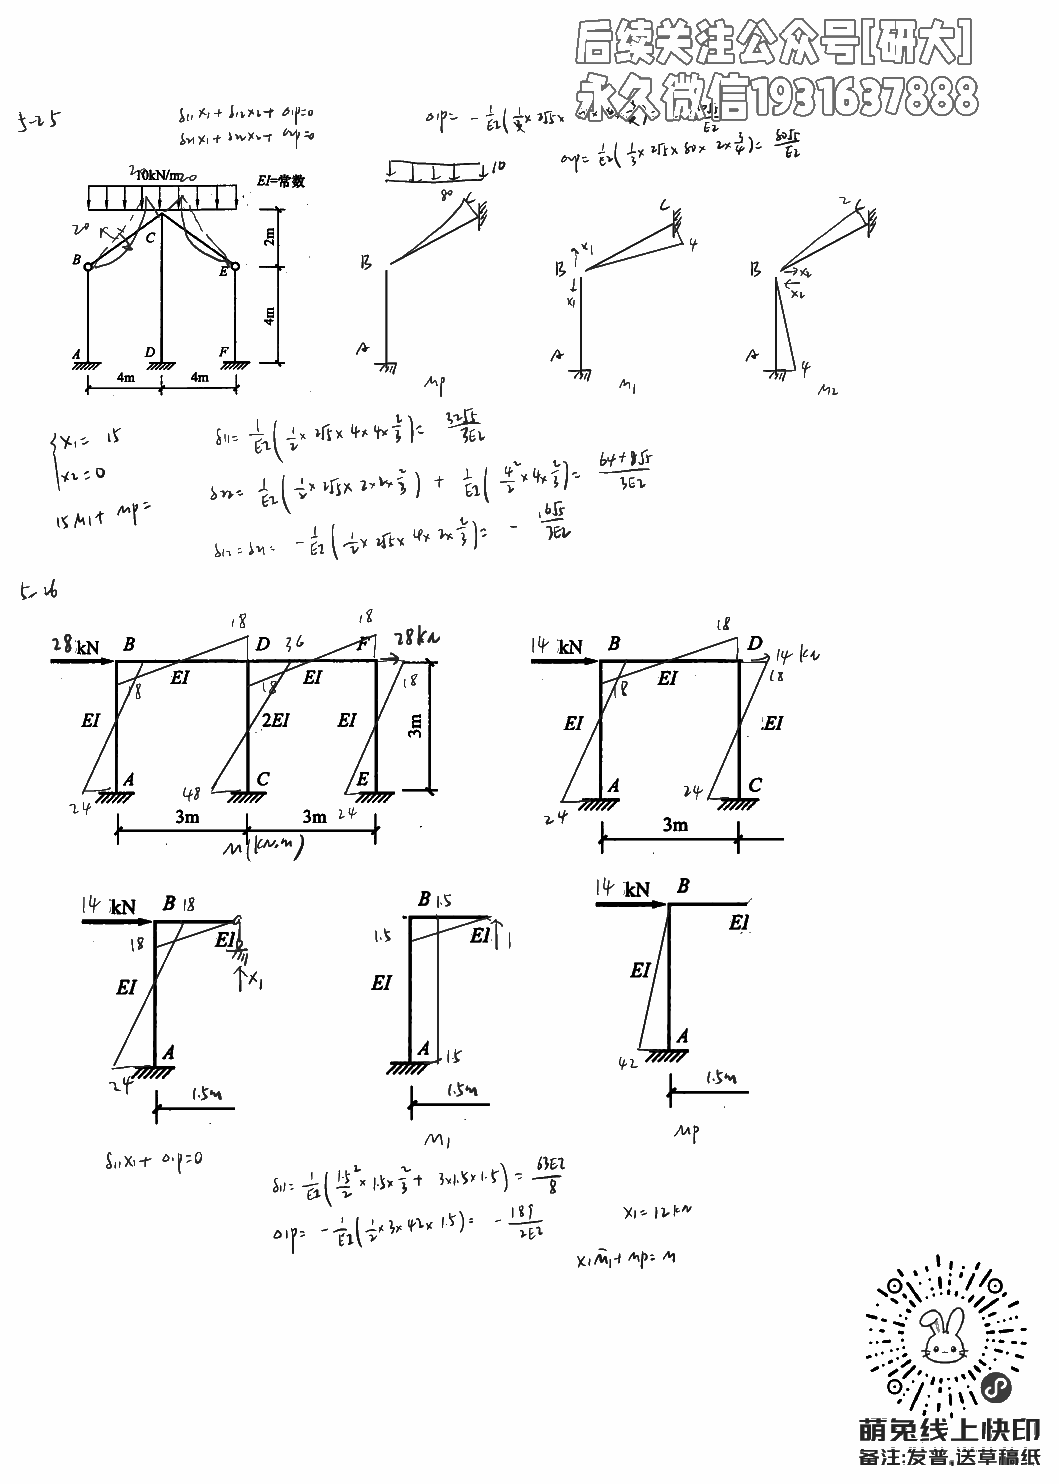
\includegraphics[width=0.96\textwidth,height=0.82\textheight,keepaspectratio]{images/c11_note_p13.png}
\par\small 讲解笔记（去水印版），第 13/21 页
\end{center}
\clearpage
\begin{center}
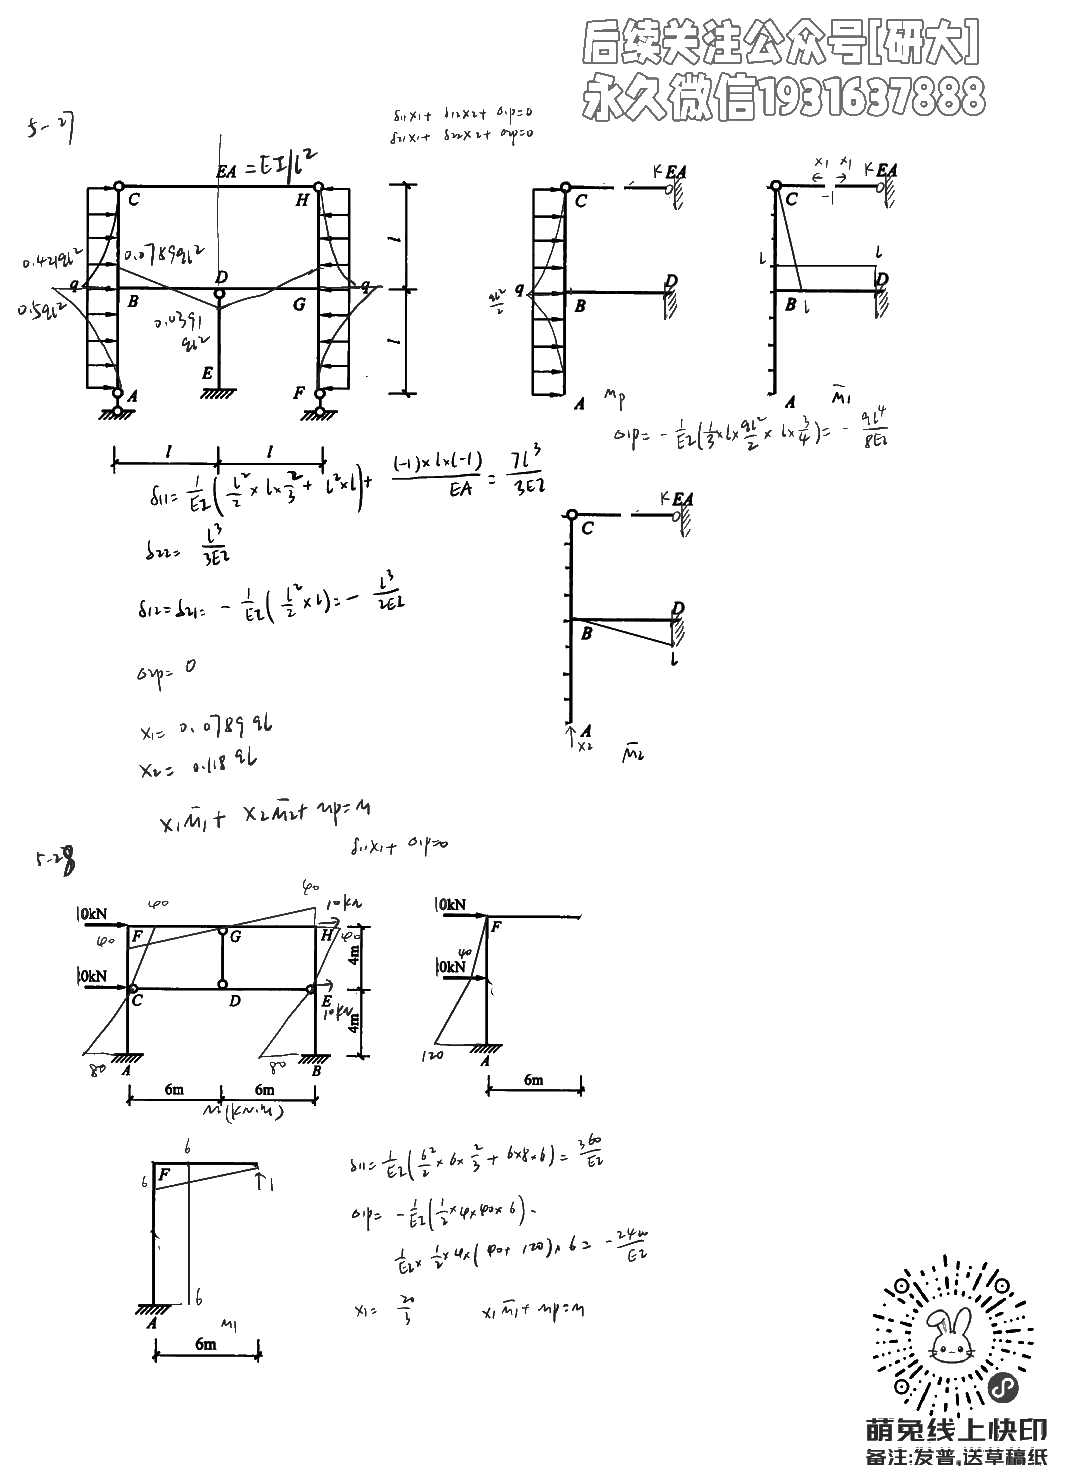
\includegraphics[width=0.96\textwidth,height=0.82\textheight,keepaspectratio]{images/c11_note_p14.png}
\par\small 讲解笔记（去水印版），第 14/21 页
\end{center}
\clearpage
\begin{center}
\includegraphics[width=0.96\textwidth,height=0.82\textheight,keepaspectratio]{images/c11_note_p15.png}
\par\small 讲解笔记（去水印版），第 15/21 页
\end{center}
\clearpage
\begin{center}
\includegraphics[width=0.96\textwidth,height=0.82\textheight,keepaspectratio]{images/c11_note_p16.png}
\par\small 讲解笔记（去水印版），第 16/21 页
\end{center}
\clearpage
\begin{center}
\includegraphics[width=0.96\textwidth,height=0.82\textheight,keepaspectratio]{images/c11_note_p17.png}
\par\small 讲解笔记（去水印版），第 17/21 页
\end{center}
\clearpage
\begin{center}
\includegraphics[width=0.96\textwidth,height=0.82\textheight,keepaspectratio]{images/c11_note_p18.png}
\par\small 讲解笔记（去水印版），第 18/21 页
\end{center}
\clearpage
\begin{center}
\includegraphics[width=0.96\textwidth,height=0.82\textheight,keepaspectratio]{images/c11_note_p19.png}
\par\small 讲解笔记（去水印版），第 19/21 页
\end{center}
\clearpage
\begin{center}
\includegraphics[width=0.96\textwidth,height=0.82\textheight,keepaspectratio]{images/c11_note_p20.png}
\par\small 讲解笔记（去水印版），第 20/21 页
\end{center}
\clearpage
\begin{center}
\includegraphics[width=0.96\textwidth,height=0.82\textheight,keepaspectratio]{images/c11_note_p21.png}
\par\small 讲解笔记（去水印版），第 21/21 页
\end{center}
\clearpage
\chapter{第12讲：位移法}
\begin{tcolorbox}[title=解析要点]
位移法以结点位移和杆端转角为基本未知量。先写杆端弯矩/剪力表达式，再由结点力矩平衡或剪力平衡建立方程求位移。
\end{tcolorbox}
\begin{tcolorbox}[title=答案与校核]
答案页给出位移法作业完整解答；讲解笔记第 11 次可作为同主题补充。
\end{tcolorbox}
\section{作业与答案（去水印版）}
\begin{center}
\includegraphics[width=0.96\textwidth,height=0.82\textheight,keepaspectratio]{images/c12_answer_1_p01.png}
\par\small 作业与答案（去水印版），第 1/28 页
\end{center}
\clearpage
\begin{center}
\includegraphics[width=0.96\textwidth,height=0.82\textheight,keepaspectratio]{images/c12_answer_1_p02.png}
\par\small 作业与答案（去水印版），第 2/28 页
\end{center}
\clearpage
\begin{center}
\includegraphics[width=0.96\textwidth,height=0.82\textheight,keepaspectratio]{images/c12_answer_1_p03.png}
\par\small 作业与答案（去水印版），第 3/28 页
\end{center}
\clearpage
\begin{center}
\includegraphics[width=0.96\textwidth,height=0.82\textheight,keepaspectratio]{images/c12_answer_1_p04.png}
\par\small 作业与答案（去水印版），第 4/28 页
\end{center}
\clearpage
\begin{center}
\includegraphics[width=0.96\textwidth,height=0.82\textheight,keepaspectratio]{images/c12_answer_1_p05.png}
\par\small 作业与答案（去水印版），第 5/28 页
\end{center}
\clearpage
\begin{center}
\includegraphics[width=0.96\textwidth,height=0.82\textheight,keepaspectratio]{images/c12_answer_1_p06.png}
\par\small 作业与答案（去水印版），第 6/28 页
\end{center}
\clearpage
\begin{center}
\includegraphics[width=0.96\textwidth,height=0.82\textheight,keepaspectratio]{images/c12_answer_1_p07.png}
\par\small 作业与答案（去水印版），第 7/28 页
\end{center}
\clearpage
\begin{center}
\includegraphics[width=0.96\textwidth,height=0.82\textheight,keepaspectratio]{images/c12_answer_1_p08.png}
\par\small 作业与答案（去水印版），第 8/28 页
\end{center}
\clearpage
\begin{center}
\includegraphics[width=0.96\textwidth,height=0.82\textheight,keepaspectratio]{images/c12_answer_1_p09.png}
\par\small 作业与答案（去水印版），第 9/28 页
\end{center}
\clearpage
\begin{center}
\includegraphics[width=0.96\textwidth,height=0.82\textheight,keepaspectratio]{images/c12_answer_1_p10.png}
\par\small 作业与答案（去水印版），第 10/28 页
\end{center}
\clearpage
\begin{center}
\includegraphics[width=0.96\textwidth,height=0.82\textheight,keepaspectratio]{images/c12_answer_1_p11.png}
\par\small 作业与答案（去水印版），第 11/28 页
\end{center}
\clearpage
\begin{center}
\includegraphics[width=0.96\textwidth,height=0.82\textheight,keepaspectratio]{images/c12_answer_1_p12.png}
\par\small 作业与答案（去水印版），第 12/28 页
\end{center}
\clearpage
\begin{center}
\includegraphics[width=0.96\textwidth,height=0.82\textheight,keepaspectratio]{images/c12_answer_1_p13.png}
\par\small 作业与答案（去水印版），第 13/28 页
\end{center}
\clearpage
\begin{center}
\includegraphics[width=0.96\textwidth,height=0.82\textheight,keepaspectratio]{images/c12_answer_1_p14.png}
\par\small 作业与答案（去水印版），第 14/28 页
\end{center}
\clearpage
\begin{center}
\includegraphics[width=0.96\textwidth,height=0.82\textheight,keepaspectratio]{images/c12_answer_1_p15.png}
\par\small 作业与答案（去水印版），第 15/28 页
\end{center}
\clearpage
\begin{center}
\includegraphics[width=0.96\textwidth,height=0.82\textheight,keepaspectratio]{images/c12_answer_1_p16.png}
\par\small 作业与答案（去水印版），第 16/28 页
\end{center}
\clearpage
\begin{center}
\includegraphics[width=0.96\textwidth,height=0.82\textheight,keepaspectratio]{images/c12_answer_1_p17.png}
\par\small 作业与答案（去水印版），第 17/28 页
\end{center}
\clearpage
\begin{center}
\includegraphics[width=0.96\textwidth,height=0.82\textheight,keepaspectratio]{images/c12_answer_1_p18.png}
\par\small 作业与答案（去水印版），第 18/28 页
\end{center}
\clearpage
\begin{center}
\includegraphics[width=0.96\textwidth,height=0.82\textheight,keepaspectratio]{images/c12_answer_1_p19.png}
\par\small 作业与答案（去水印版），第 19/28 页
\end{center}
\clearpage
\begin{center}
\includegraphics[width=0.96\textwidth,height=0.82\textheight,keepaspectratio]{images/c12_answer_1_p20.png}
\par\small 作业与答案（去水印版），第 20/28 页
\end{center}
\clearpage
\begin{center}
\includegraphics[width=0.96\textwidth,height=0.82\textheight,keepaspectratio]{images/c12_answer_1_p21.png}
\par\small 作业与答案（去水印版），第 21/28 页
\end{center}
\clearpage
\begin{center}
\includegraphics[width=0.96\textwidth,height=0.82\textheight,keepaspectratio]{images/c12_answer_1_p22.png}
\par\small 作业与答案（去水印版），第 22/28 页
\end{center}
\clearpage
\begin{center}
\includegraphics[width=0.96\textwidth,height=0.82\textheight,keepaspectratio]{images/c12_answer_1_p23.png}
\par\small 作业与答案（去水印版），第 23/28 页
\end{center}
\clearpage
\begin{center}
\includegraphics[width=0.96\textwidth,height=0.82\textheight,keepaspectratio]{images/c12_answer_1_p24.png}
\par\small 作业与答案（去水印版），第 24/28 页
\end{center}
\clearpage
\begin{center}
\includegraphics[width=0.96\textwidth,height=0.82\textheight,keepaspectratio]{images/c12_answer_1_p25.png}
\par\small 作业与答案（去水印版），第 25/28 页
\end{center}
\clearpage
\begin{center}
\includegraphics[width=0.96\textwidth,height=0.82\textheight,keepaspectratio]{images/c12_answer_1_p26.png}
\par\small 作业与答案（去水印版），第 26/28 页
\end{center}
\clearpage
\begin{center}
\includegraphics[width=0.96\textwidth,height=0.82\textheight,keepaspectratio]{images/c12_answer_1_p27.png}
\par\small 作业与答案（去水印版），第 27/28 页
\end{center}
\clearpage
\begin{center}
\includegraphics[width=0.96\textwidth,height=0.82\textheight,keepaspectratio]{images/c12_answer_1_p28.png}
\par\small 作业与答案（去水印版），第 28/28 页
\end{center}
\clearpage
\section{讲解笔记（去水印版）}
\begin{center}
\includegraphics[width=0.96\textwidth,height=0.82\textheight,keepaspectratio]{images/c12_note_p01.png}
\par\small 讲解笔记（去水印版），第 1/21 页
\end{center}
\clearpage
\begin{center}
\includegraphics[width=0.96\textwidth,height=0.82\textheight,keepaspectratio]{images/c12_note_p02.png}
\par\small 讲解笔记（去水印版），第 2/21 页
\end{center}
\clearpage
\begin{center}
\includegraphics[width=0.96\textwidth,height=0.82\textheight,keepaspectratio]{images/c12_note_p03.png}
\par\small 讲解笔记（去水印版），第 3/21 页
\end{center}
\clearpage
\begin{center}
\includegraphics[width=0.96\textwidth,height=0.82\textheight,keepaspectratio]{images/c12_note_p04.png}
\par\small 讲解笔记（去水印版），第 4/21 页
\end{center}
\clearpage
\begin{center}
\includegraphics[width=0.96\textwidth,height=0.82\textheight,keepaspectratio]{images/c12_note_p05.png}
\par\small 讲解笔记（去水印版），第 5/21 页
\end{center}
\clearpage
\begin{center}
\includegraphics[width=0.96\textwidth,height=0.82\textheight,keepaspectratio]{images/c12_note_p06.png}
\par\small 讲解笔记（去水印版），第 6/21 页
\end{center}
\clearpage
\begin{center}
\includegraphics[width=0.96\textwidth,height=0.82\textheight,keepaspectratio]{images/c12_note_p07.png}
\par\small 讲解笔记（去水印版），第 7/21 页
\end{center}
\clearpage
\begin{center}
\includegraphics[width=0.96\textwidth,height=0.82\textheight,keepaspectratio]{images/c12_note_p08.png}
\par\small 讲解笔记（去水印版），第 8/21 页
\end{center}
\clearpage
\begin{center}
\includegraphics[width=0.96\textwidth,height=0.82\textheight,keepaspectratio]{images/c12_note_p09.png}
\par\small 讲解笔记（去水印版），第 9/21 页
\end{center}
\clearpage
\begin{center}
\includegraphics[width=0.96\textwidth,height=0.82\textheight,keepaspectratio]{images/c12_note_p10.png}
\par\small 讲解笔记（去水印版），第 10/21 页
\end{center}
\clearpage
\begin{center}
\includegraphics[width=0.96\textwidth,height=0.82\textheight,keepaspectratio]{images/c12_note_p11.png}
\par\small 讲解笔记（去水印版），第 11/21 页
\end{center}
\clearpage
\begin{center}
\includegraphics[width=0.96\textwidth,height=0.82\textheight,keepaspectratio]{images/c12_note_p12.png}
\par\small 讲解笔记（去水印版），第 12/21 页
\end{center}
\clearpage
\begin{center}
\includegraphics[width=0.96\textwidth,height=0.82\textheight,keepaspectratio]{images/c12_note_p13.png}
\par\small 讲解笔记（去水印版），第 13/21 页
\end{center}
\clearpage
\begin{center}
\includegraphics[width=0.96\textwidth,height=0.82\textheight,keepaspectratio]{images/c12_note_p14.png}
\par\small 讲解笔记（去水印版），第 14/21 页
\end{center}
\clearpage
\begin{center}
\includegraphics[width=0.96\textwidth,height=0.82\textheight,keepaspectratio]{images/c12_note_p15.png}
\par\small 讲解笔记（去水印版），第 15/21 页
\end{center}
\clearpage
\begin{center}
\includegraphics[width=0.96\textwidth,height=0.82\textheight,keepaspectratio]{images/c12_note_p16.png}
\par\small 讲解笔记（去水印版），第 16/21 页
\end{center}
\clearpage
\begin{center}
\includegraphics[width=0.96\textwidth,height=0.82\textheight,keepaspectratio]{images/c12_note_p17.png}
\par\small 讲解笔记（去水印版），第 17/21 页
\end{center}
\clearpage
\begin{center}
\includegraphics[width=0.96\textwidth,height=0.82\textheight,keepaspectratio]{images/c12_note_p18.png}
\par\small 讲解笔记（去水印版），第 18/21 页
\end{center}
\clearpage
\begin{center}
\includegraphics[width=0.96\textwidth,height=0.82\textheight,keepaspectratio]{images/c12_note_p19.png}
\par\small 讲解笔记（去水印版），第 19/21 页
\end{center}
\clearpage
\begin{center}
\includegraphics[width=0.96\textwidth,height=0.82\textheight,keepaspectratio]{images/c12_note_p20.png}
\par\small 讲解笔记（去水印版），第 20/21 页
\end{center}
\clearpage
\begin{center}
\includegraphics[width=0.96\textwidth,height=0.82\textheight,keepaspectratio]{images/c12_note_p21.png}
\par\small 讲解笔记（去水印版），第 21/21 页
\end{center}
\clearpage
\chapter{第13讲：弯矩分配法}
\begin{tcolorbox}[title=解析要点]
弯矩分配法适合无侧移或经处理后的连续梁、刚架。步骤是计算转动刚度、分配系数、固端弯矩，然后反复分配与传递直至收敛。
\end{tcolorbox}
\begin{tcolorbox}[title=答案与校核]
答案页给出弯矩分配过程；可用结点不平衡力矩逐轮趋近零进行检查。
\end{tcolorbox}
\section{作业与答案（去水印版）}
\begin{center}
\includegraphics[width=0.96\textwidth,height=0.82\textheight,keepaspectratio]{images/c13_answer_1_p01.png}
\par\small 作业与答案（去水印版），第 1/4 页
\end{center}
\clearpage
\begin{center}
\includegraphics[width=0.96\textwidth,height=0.82\textheight,keepaspectratio]{images/c13_answer_1_p02.png}
\par\small 作业与答案（去水印版），第 2/4 页
\end{center}
\clearpage
\begin{center}
\includegraphics[width=0.96\textwidth,height=0.82\textheight,keepaspectratio]{images/c13_answer_1_p03.png}
\par\small 作业与答案（去水印版），第 3/4 页
\end{center}
\clearpage
\begin{center}
\includegraphics[width=0.96\textwidth,height=0.82\textheight,keepaspectratio]{images/c13_answer_1_p04.png}
\par\small 作业与答案（去水印版），第 4/4 页
\end{center}
\clearpage
\section{讲解笔记（去水印版）}
\begin{tcolorbox}[title=缺失说明]
当前目录未找到对应 PDF。
\end{tcolorbox}
\clearpage
\chapter{第14讲：矩阵位移法}
\begin{tcolorbox}[title=解析要点]
矩阵位移法按单元刚度矩阵、坐标变换、总体刚度组装、施加边界条件、解结点位移、回代单元内力的流程完成。
\end{tcolorbox}
\begin{tcolorbox}[title=答案与校核]
答案页给出矩阵位移法作业结果；讲解笔记第 13 次补充了矩阵组装和回代思路。
\end{tcolorbox}
\section{作业与答案（去水印版）}
\begin{center}
\includegraphics[width=0.96\textwidth,height=0.82\textheight,keepaspectratio]{images/c14_answer_1_p01.png}
\par\small 作业与答案（去水印版），第 1/4 页
\end{center}
\clearpage
\begin{center}
\includegraphics[width=0.96\textwidth,height=0.82\textheight,keepaspectratio]{images/c14_answer_1_p02.png}
\par\small 作业与答案（去水印版），第 2/4 页
\end{center}
\clearpage
\begin{center}
\includegraphics[width=0.96\textwidth,height=0.82\textheight,keepaspectratio]{images/c14_answer_1_p03.png}
\par\small 作业与答案（去水印版），第 3/4 页
\end{center}
\clearpage
\begin{center}
\includegraphics[width=0.96\textwidth,height=0.82\textheight,keepaspectratio]{images/c14_answer_1_p04.png}
\par\small 作业与答案（去水印版），第 4/4 页
\end{center}
\clearpage
\section{讲解笔记（去水印版）}
\begin{center}
\includegraphics[width=0.96\textwidth,height=0.82\textheight,keepaspectratio]{images/c14_note_p01.png}
\par\small 讲解笔记（去水印版），第 1/10 页
\end{center}
\clearpage
\begin{center}
\includegraphics[width=0.96\textwidth,height=0.82\textheight,keepaspectratio]{images/c14_note_p02.png}
\par\small 讲解笔记（去水印版），第 2/10 页
\end{center}
\clearpage
\begin{center}
\includegraphics[width=0.96\textwidth,height=0.82\textheight,keepaspectratio]{images/c14_note_p03.png}
\par\small 讲解笔记（去水印版），第 3/10 页
\end{center}
\clearpage
\begin{center}
\includegraphics[width=0.96\textwidth,height=0.82\textheight,keepaspectratio]{images/c14_note_p04.png}
\par\small 讲解笔记（去水印版），第 4/10 页
\end{center}
\clearpage
\begin{center}
\includegraphics[width=0.96\textwidth,height=0.82\textheight,keepaspectratio]{images/c14_note_p05.png}
\par\small 讲解笔记（去水印版），第 5/10 页
\end{center}
\clearpage
\begin{center}
\includegraphics[width=0.96\textwidth,height=0.82\textheight,keepaspectratio]{images/c14_note_p06.png}
\par\small 讲解笔记（去水印版），第 6/10 页
\end{center}
\clearpage
\begin{center}
\includegraphics[width=0.96\textwidth,height=0.82\textheight,keepaspectratio]{images/c14_note_p07.png}
\par\small 讲解笔记（去水印版），第 7/10 页
\end{center}
\clearpage
\begin{center}
\includegraphics[width=0.96\textwidth,height=0.82\textheight,keepaspectratio]{images/c14_note_p08.png}
\par\small 讲解笔记（去水印版），第 8/10 页
\end{center}
\clearpage
\begin{center}
\includegraphics[width=0.96\textwidth,height=0.82\textheight,keepaspectratio]{images/c14_note_p09.png}
\par\small 讲解笔记（去水印版），第 9/10 页
\end{center}
\clearpage
\begin{center}
\includegraphics[width=0.96\textwidth,height=0.82\textheight,keepaspectratio]{images/c14_note_p10.png}
\par\small 讲解笔记（去水印版），第 10/10 页
\end{center}
\clearpage
\backmatter
\chapter*{源文件索引}
\begin{itemize}
\item 第1讲：作业/答案：结构力学基础与技巧班第1次作业答案（几何组成分析）.pdf；结构力学基础与技巧班第1次作业（几何组成分析）.pdf；讲解笔记：【第1次作业笔记】—几何组成分析.pdf。
\item 第2讲：作业/答案：结构力学基础与技巧班第2次作业答案（理论力学回顾）.pdf；结构力学基础与技巧班第2次作业（理论力学回顾）.pdf；讲解笔记：【第2次作业笔记】—理论力学回顾.pdf。
\item 第3讲：作业/答案：结构力学基础与技巧班第3次作业答案（材料力学回顾）.pdf；结构力学基础与技巧班第3次作业（材料力学回顾）.pdf；讲解笔记：【第3次作业笔记】—材料力学回顾.pdf。
\item 第4讲：作业/答案：结构力学基础与技巧班第4次作业及答案（静定梁和刚架）.pdf；讲解笔记：【第4次作业笔记】—梁和刚架.pdf。
\item 第5讲：作业/答案：结构力学基础与技巧班第5次作业及答案（静定桁架）.pdf；讲解笔记：【第5次作业笔记】—静定桁架.pdf。
\item 第6讲：作业/答案：结构力学基础与技巧班第6次作业及答案（组合结构）.pdf；讲解笔记：【第6次作业笔记】—组合结构.pdf。
\item 第7讲：作业/答案：结构力学基础与技巧班第7次作业及答案（三铰拱）.pdf；讲解笔记：【第7次作业笔记】—拱结构.pdf。
\item 第8讲：作业/答案：结构力学基础与技巧班第8次作业及答案（静定结构影响线）.pdf；讲解笔记：【第8次作业笔记】—影响线.pdf。
\item 第9讲：作业/答案：结构力学基础与技巧班第9次作业及答案（静定结构位移计算）.pdf；讲解笔记：【第9次作业笔记】—位移计算.pdf。
\item 第10讲：作业/答案：结构力学基础与技巧班第10次作业及答案（力法1）.pdf；讲解笔记：【第10次作业笔记】—力法.pdf。
\item 第11讲：作业/答案：结构力学基础与技巧班第11次作业及答案（力法2）.pdf；讲解笔记：【第10次作业笔记】—力法.pdf。
\item 第12讲：作业/答案：结构力学基础与技巧班第12次作业及答案（位移法）.pdf；讲解笔记：【第11次作业笔记】—位移法.pdf。
\item 第13讲：作业/答案：结构力学基础与技巧班第13次作业及答案（弯矩分配法）.pdf；讲解笔记：未找到。
\item 第14讲：作业/答案：结构力学基础与技巧班第14次作业及答案（矩阵位移法）.pdf；讲解笔记：【第13次作业笔记】—矩阵位移法.pdf。
\end{itemize}
\end{document}
